% Autor: Betti Oesterholz
% erstellt: 05.03.2008
% Haupdokument Fib umfangreich V1.0
% Dies ist das Haupdokument der der umfangreichen, deutschen
% Fib -Dokumentation.
%
% Copyright (c) 2008 Betti Oesterholz
%
% Permission is granted to copy, distribute and/or modify this document
% under the terms of the GNU Free Documentation License, Version 1.2 or
% any later version published by the Free Software Foundation;
% with no Invariant Sections, no Front-Cover Texts, and no Back-Cover Texts.
%
% A copy of the license is included in the file ``fdl.tex'' .
%



\documentclass[11pt,a4paper]{article}
\usepackage{ngerman} % Silbentrennung nach neuer Rechtschreibung
\usepackage[T1]{fontenc} % Type 1 Schriften
\usepackage{times} % Da die Standard-LaTeX-Schrift bei mir mit Acrobat nicht funkt.
\usepackage[ansinew]{inputenc} % Verwendung von Umlauten
\usepackage{scrpage2} % Seitenformat
\usepackage{titletoc}
\usepackage{titlesec}
\usepackage{listings} % Programm-Listing
%\usepackage [usetoc]{titleref} 
\usepackage{graphicx} % Einbindung von Graphiken
\usepackage{url} % URLs durch \url{}
\usepackage{bibgerm} % deutsche Bibliographie
%\usepackage{txfonts}%Paket fr das nat Symbol
\usepackage{multicol}
\usepackage{makeidx}%for the index
\usepackage{longtable}
%\usepackage{amsmath}%mathematikumgebung {equation*} usw.

% Seitenstil festlegen
\pagestyle{useheadings}%or: headings

% n�hste vier Zeilen: Format des Inhaltsverzeichnisses
%\titlespacing{\section}{0pt}{5cm}{5cm}%spacing by sections {in front}{above}{below}
%\dottedcontents{section}[1.5em]{\addvspace{1.0em}}{1.3em}{0.7pc}
%\dottedcontents{subsection}[3.8em]{}{2.2em}{0.7pc}
%\dottedcontents{subsubsection}[7.0em]{}{3.1em}{0.7pc}

%\setcounter{secnumdepth}{4}%%nummerierung der Unterabschnitte bis Tiefe

%Pfad fuer Bilder
\graphicspath{{images}{./material_grundlagen/}}


%%%%%%%%%%%%%%%%%%%%%%%%%%%%%%%%%%%%%%%%%%%%%%%%%%%%%%%%%%%%%%%%%%%%%%%%%%%%%%%%%%%%%%%
% Definitionen fr das Verwenden von Listings

\newtheorem{Def}{Definition}

%%%%%%%%%%%%%%%%%%%%%%%%%%%%%%%%%%%%%%%%%%%%%%%%%%%%%%%%%%%%%%%%%%%%%%%%%%%%%%%%%%%%%%%
% Beginn des Dokuments

\makeindex 

\begin{document}

\setlength{\unitlength}{1cm} %definition of the basislength in pictures

\title{Das Fib -Multimediaformat}
\author{Betti Österholz}
\date{\today}

\begin{titlepage}
	\begin{center}
	\ \vspace{2.5cm} \\
	\Huge\bf Das Fib -Multimediaformat\\\vspace{3cm}
	\LARGE Betti Österholz\\\vspace{0.5cm}
	\large BioKom@gmx.de\\\vspace{0.5cm}
	\large www.BioKom.info\\\vspace{0.5cm}
	Potsdam, \today\\\vspace{5.5cm}
	\end{center}
	
	\noindent
Copyright (c) 2010  Betti Österholz
\newline\newline
Permission is granted to copy, distribute and/or modify this document under the terms of the GNU Free Documentation License, Version 1.2 or any later version published by the Free Software Foundation; with no Invariant Sections, no Front-Cover Texts, and no Back-Cover Texts.

A copy of the license is included in the section entitled "`GNU Free Documentation License"'.
\end{titlepage}

\renewcommand{\sectionmark}[1]{\markboth{#1}{}}
\pagenumbering {Roman}
\automark{section}
\pagestyle{scrheadings} % individ. Seitenlayout
\setheadsepline{0.4pt}
\ihead{} % Titelzeile innen
\ohead{} % Titelzeile aussen
\chead{\slshape \headmark}  % Titelzeile mitte
\cfoot{\thepage} % Fusszeile mitte

% braucht man ein Inhaltsverzeichnis, so sind die n�hsten drei Zeilen auszukommentieren
%\setcounter{tocdepth}{3}
%\tableofcontents
%\clearpage

% Vorschlag fr Titelzeile:
% Bei umfangreicheren Dokumenten
\ihead{\slshape \headmark } % Darstellung von Sectionnummer und -name
\ohead{}
\chead{}
\clearpage

\tableofcontents

\clearpage
\pagenumbering{arabic}

\part{Einleitung}

Das Fib -Multimediaformat dient zum Speichern von Multimediainformationen in strukturierter, funktionaler und hierarchischer Form. Die Struktur der Fib- Multimediaformat unterstützt die Objektsicht auf Dinge. Das Fib -Multimediaformat ist sehr mächtig, da Ausdrücke kombiniert und verschachtelt werden können. Der Speicheraufwand eines Multimediobjekts in Fib ist vielmehr von dessen Komplexität abhängig als von dessen Größe (im Sinne von Ausdehnung in den Dimension, also Beispielsweise die Höhe und Breite bei Bildern) wie bei üblichen Speicherformaten.

Die zweite wichtige Komponente des Fib -Systems ist der genetische Algorithmus zum Kodieren in und Komprimieren von Fib -Multimediaobjekten. Der große Vorteil dieses ist, dass die Kodierung und Komprimierung nicht mehr an einem bestimmten Algorithmus gebunden ist, sondern dass die eigendlichen Kodierungs- und Komprimierungsalgorithmen im genetischen Algorithmus als Operationen eingebunden werden, welche leicht hinzugefügt und geändert werden können. Dadurch ist es leicht neue Kodierungs- und Komprimierungsideen einzubringen und eine Vielzahl von diesen auf ein Multimediaobjekt anzuwenden.

In diesem Sinne baut das Fib -Multimediasystem auf Vielfalt und nicht auf Spezialisierung auf.


\section{Der Ausgangspunkt}

Ein (natürliches) Bild besteht im allgemeinen nicht aus einer Aneinanderreihung zusammenhangloser Pixel (Punkte mit bestimmten Farben), sondern zeigt z.B. Objekte die gegeneinander abgegrenzt sind und eine Textur haben. Solche Objekte (z.B. Kreise, Linien aber auch komplexere Objekte) wiederholen sich oftmals auf Bildern, sei es als selbstähnliche Kopie oder transformierte Kopie (z.B. Blätter von Bäumen oder Latten im Lattenzaun). Das Gleiche gilt für andere Inhalte von Multimediadaten, wie den Ton.

Des weiteren können Elemente die durch Multimediadaten gezeigt werden sollen oft miteinander assoziiert oder gruppiert werden, z.B. gehören Geräusche oft zu bestimmten dargestellten Objekten (z.B. Entenschnabel), Objekt gehören zu andern Objekten (z.B. Entenschnabel zur Ente) und mehrere Objekte  können zu einem Objekt (z.B. eine Wiese mit einer Entengruppe) gruppiert werden.


\section{Problem}
\label{secProblem}

Wie können Informationen über Objekte aus einem Bild extrahieren werden, das in Form einer Matrix von Pixeln gegeben ist? (Das Bild ist als Pixelbild gegeben, weil es Beispielsweise durch Digitalfotografie über einem Fotochip aufgenommen wurde.)

Diese extrahierten Information kann dann z.B. zur Komprimierung benutzt werden, da die Informationen, die benötigt werden um ein Objekt zu kodieren, maximal die Informationen aller Punkte des Objekts mit ihren Farben entspricht (diese Kodierung ist ja gegeben). Wird Beispielsweise ein grünes Dreieck im Bild gefunden, das aus 200 grünen Punkten besteht, reicht es im Idealfall einfach das Dreieck bzw. die Punkte durch ein Dreieckobjekt darzustellen, für dass nur seine drei Ecken und seine Farbe benötigt werden.

Man kann mit Information über Objekte im Bild aber auch Objekte auf anderen (Teil-) Bildern wiedererkennen. Oder die Informationen können genutzt werden, um das Bild zu manipulieren, z.B. um Objekte als Ganzes zu entfernen, kopieren oder einzufügen.


\section{Lösungsidee}
\label{secSolution}

Es wird eine ``Multimediasprache'' definiert, in der Objekte, Transformationen und Zusammenhänge zwischen diesen definieren werden können. Mit Hilfe dieser entwirft ein Algorithmus (z.B. aus der KI) dann Programme (in der Multimediasprache), testet und verändert diese, so dass sie ein Multimediaobjekt darstellen, das dem zu kodierendem Multimediaobjekt ähnlich genug ist (was dies ist, sollte spezifiziert werden). Dabei können an dieses Programm noch weitere Einschränkungen gestellt werden, z.B. Kürze und Abarbeitungsgeschwindigkeit des Programms. Mit diesen Kriterien kann dann feststellen werden, wie ``gut'' das Programm ist.

Unter anderem bieten sich dafür genetische Algorithmen/Programmierung an. Da bei genetischen Algorithmen die einzelnen Parameter, Elemente und Konstrukte der Sprache durch Mutation erzeugt und angepasst werden können und die ``besten'' Programme weiterentwickelt werden. Mit ``crossing over'', Austausch von Programmcode zwischen Programmen oder Programmstellen, kann der Umstand berücksichtigt werden, dass die Objekte an anderen Stellen eventuell nur verändert (z.B. vergrößert) wiederverwendet werden.


\section{This document ...}




\section{Einteilung dieses Projekts}

Der Aufbau dieses Dokuments richtet sich nach der Projektstruktur.

Das Projekt is hirarchisch aufgebaut und gliedert sich in zwei große Komponenten.
Die Komponenten sind die Multimediabeschreibungssprache Fib und der genetische Algorithmus, um effizente Fib -Kodierungen von Multimediaobjekten zu erzeugen.

Hirarchisch ist das Projekt, also auch je die Komponenten, in mehrere Ebenen aufgebaut, wobei eine höhere Ebene auf den unteren Aufbauen. Wobei die Ebenen dabei immer detailierter werden.
\bigskip\noindent
Diese Ebenen sind:
\begin{enumerate}
 \item Eine Zielbeschreibung der Komponenten (siehe Abschnitt \ref{secProblem} auf Seite \pageref{secProblem}, sowie den folgenden Abschnitt \ref{secSolution} und für Fib Abschnitt \ref{secFibLanguageRequirements} auf Seite \pageref{secFibLanguageRequirements} )
 \item Die theoretische Beschreibung der Komponente: Diese beschreibt die Komponenten ohne auf deren möglich Realisierung einzugehen. (siehe für die Fib -Sprache Abschnitt \ref{partFibLanguage} auf Seite \pageref{partFibLanguage} und für den denetischen Algorithmus Abschnitt \ref{secGeneticAlgorithmDesign} auf Seite \pageref{secGeneticAlgorithmDesign} )
 \item Einen Entwurf der Realisierung der Komponente: Dies ist ein Entwurf für die Implementierung der Komponenten. Er kann von der tatsächlichen Implementierung abweichen und soll nur den algemeinen Aufbau sowie die Schnittstellen beschreiben. Implementierungen sollten sich nach diesem richten, so dass sie auf einem allgemeinen Standard fußen. Der Entwurf sollte aber Implementierungen genug weitere Freiräume lassen. (siehe Allgemein Abschnitt \ref{partFibProjectstructurImplementation} auf Seite \pageref{partFibProjectstructurImplementation}; für die Fib -Sprache Abschnitt \ref{partImplementationFib} auf Seite \pageref{partImplementationFib} und Abschnitt \ref{partFileFormat} auf Seite \pageref{partFileFormat}; sowie für den denetischen Algorithmus Abschnitt \ref{partImplementationAlgorithmus} auf Seite \pageref{partImplementationAlgorithmus}, Abschnitt \ref{partImplementationAlgorithmusFib} auf Seite \pageref{partImplementationAlgorithmusFib} und Abschnitt \ref{partFibOperations} auf Seite \pageref{partFibOperations})
 \item Die Dokumentation der Realisierung: Sie umfast die Beschreibung der Schnittstellen der konkreten Implementierung. Eine solche Dokumentation ist nicht in diesem Dokument enthalten und ist zur jeweiligen Realisierung zu halten. In der konkreten Realisierung in C++ zu diesem Dokument, gibt es eine Dokumentation die mit Doxygen erstellt wird und im Doxygen Java Stil erfolgt.
 \item Die konkrete Realisierungen: Auch hier ist eine Dokumentation der Funktionsweise des Quellcodes sinnvoll.
\end{enumerate}



\section{Einteilung dieses Dokuments}

In diesem Abschnitt wird eine Übersicht über den Inhalt und Aufbau dieses Dokuments gegeben.


%TODO Anpassen und Erweitern


\subsection{Entwurf der Multimediabeschreibungssprache}

Der Teil \ref{partFibLanguage} auf Seite \pageref{partFibLanguage} befasst sich mit der Multimediabeschreibungssprache.

In Abschnitt \ref{secFibElements} auf Seite \pageref{secFibElements} werden die einzelnen Elemente und deren mögliche Beziehungen zueinander spezifiziert.

Der Abschnitt \ref{secFibDatabase} auf Seite \pageref{secFibDatabase} geht auf die Datenbankfunktion für Fib (-Objekte) ein.

Im nachfolgenden Abschnitt \ref{secDefinitionsForFib} auf Seite \pageref{secDefinitionsForFib} werden Definitionen für die Fib -Multimediasprache aufgestellt, die einen Umgang mit ihr erleichtern sollen.



\subsection{Entwurf des genetischen Algorithmus}

Im Teil \ref{secGeneticAlgorithmDesign} auf Seite \pageref{secGeneticAlgorithmDesign} wird der Entwurf des genetische Algorithmus beschrieben. Dabei geht es vor allem um die grundlegenden Ideen hinter dem genetische Algorithmus.


\subsection{Dateiformat}

Im Teil \ref{partFileFormat} auf Seite \pageref{partFileFormat} werden die Dateiformate für die Fib -Multimediasprache dargestellt. Diese sind unabhängig vom Programmsystem oder der Rechnerarchitektur.



%TODO einkommentieren

%%
% Copyright (c) 2008 Betti "Osterholz
%
% Permission is granted to copy, distribute and/or modify this document
% under the terms of the GNU Free Documentation License, Version 1.2 or
% any later version published by the Free Software Foundation;
% with no Invariant Sections, no Front-Cover Texts, and no Back-Cover Texts.
%
% A copy of the license is included in the file ``fdl.tex'' .
%

%Pfad fuer Bilder
\graphicspath{{./material_grundlagen/}}
\graphicspath{{./material_grundlagen/}{../material_grundlagen}}

\newpage
\part{Einf"uhrung in die Grundlagen}
\label{partIntroductionBasics}



\section{Grundlagen genetischer Algorithmen}

Evolution ist eines der grundlegensten Naturgesetze unseres Universums. Seit rund 3 Milliarden Jahren gibt es auf der Erde eine genetische Evolution, die, wie wohl nur wenige bestreiten werden, ganz erstaunliche Ergebnisse und Probleml"osungen hervorgebracht hat. Deshalb ist es nicht verwunderlich, dass versucht wird, die Methoden und/oder die Wirkungsweise der genetischen Evolution auch in der Informationstechnik einzusetzen. Vielfach werden schon gro"se Fortschritte in der Wissenschaft und Forschung erzielt, indem man sich Prinzipien der Ergebnisse (z. B. Fl"ugelauftrieb) der nat"urlichen Evolution von der Natur ``abgeschaut'' hat. Aber auch viele Interpretationen der Evolution wurden schon, teilweise mit Erfolg, versucht anzuwenden.

Die nachfolgende Arbeit ist einer dieser Versuche.

Wie funktioniert Evolution aber oder was ist sie "uberhaupt genau?

Ob ich diese Fragen zufriedenstellend beantworten kann, wei"s ich nicht. Ich will es aber versuchen und vielleicht noch ein paar Denkanst"o"se geben. Die nachfolgende Sicht von Evolution und genetischer Evolution ist grundlegend f"ur die gesamte vorliegende Arbeit. Sie nimmt aber keinesfalls in Anspruch, vollst"andig oder ``richtig'' zu sein. Um genetische Evolution verstehen zu k"onnen, muss wahrscheinlich zuerst erkl"art werden, was Evolution ist.


\subsection{Geschichte}

Der ber"uhmteste Forscher, der auf die Evolution aufmerksam wurde und dar"uber eine Buch verfasste, war Charles Darwin (1809- 1882), der 1859 das Buch ``Die Entstehung der Arten''\cite{EACD} ver"offentlichte. Dabei ging es um die Evolution in der Natur und wie Arten aus anderen Arten entstanden sind. Eine Idee, die ihm besonders im Kreise der damals noch wesentlich m"achtigeren Kirche viele Unsympathien einbrachte, da diese Idee dem Sch"opfungsgedanken zuwiderlief.

Die Idee, Evolution auch zum maschinellen Lernen zu verwenden, war sehr fr"uh in der Informatik vorhanden. Schon 1932 beschrieb W. D. Cannon nat"urliche Evolution als einen Lernprozess. A. M. Turing (1950) vermutete ``an obvious connection between $[$machine learning$]$ and evolution'' ("Ubersetzung: ``eine offensichtliche Verbindung zwischen $[$maschinellem Lernen$]$ und Evolution''). Leider war zu dieser Zeit die Rechnerleistung bei weitem noch nicht hoch genug, um eine Simulation der Evolution in vern"unftigem Rahmen zu gew"ahrleisten.
%TODO cite

Erst in den 1980ern war die zur Verf"ugung stehende Rechenleistung hoch genug, um Evolution zum maschinellen Lernen sinnvoll einsetzen zu k"onnen. Danach wurde das Interesse an Evolution in der Informatik gr"o"ser. Evolution wurde schon in vielen Bereichen mehr oder weniger erfolgreich eingesetzt. Angefangen vom Finden globaler/lokaler Optima von Funktionen, bis hin zum automatischem Schaltungsentwurf oder Roboterkonstruktion.


\subsection{Evolution}

Evolution ist ein allgemeines Prinzip/Naturgesetz, das man kurz mit ``Das Bessere setzt sich durch'' erkl"aren kann. Bei genauerer Betrachtung wird der Spruch etwas undeutlich, denn was ist ``besser'' (f"ur wen) und was ist ``sich'' oder ``durchsetzen''.

``Sich'' kann auf alles bezogen werden. Ob es nun ein Lebewesen, ein Programm, ein Prinzip oder Sonstiges ist. F"ur ``sich'' sind aber die Informationen die es enth"alt (z. B. Aufbau der Molek"ule oder Art des Gemeinschaftslebens) und nicht seine Materie oder Energie (wenn vorhanden) f"ur die Evolution ausschlaggebend. Ein Hund ist nicht so erfolgreich, weil er 25 Kilogramm Materie enth"alt, sondern weil diese Materie ( und seine Energie, wenn diese von Materie getrennt wird) auf ganz spezielle Weise ``verteilt/aufgebaut'' ist. Auch darf ``sich'' nicht als ein abgeschlossenes Einzelnes gesehen werden, sondern muss die Umwelt mit einbeziehen. Ameisen sind z. B. so erfolgreich, weil sie in Staaten leben. ``Sich'' kann auch weitere ``sichs'' enthalten oder in einem ``sich'' enthalten sein. So haben viele S"augetiere Darmbakterien, ohne die sie nicht mehr die gleichen Tiere w"aren. Viele Arten bestehen nur aufgrund dieser Darmbakterien, z. B. K"uhe.

Die Frage ``F"ur wen besser?'' muss mit ``F"ur sich besser'' beantwortet werden. ``F"ur sich besser'' ist, wenn ``sich'' h"aufiger oder wahrscheinlicher wird. 

Damit ist auch gleich die Frage beantwortet, was ``durchsetzen'' ist: Etwas setzt ``sich'' durch, wenn es wahrscheinlicher/h"aufiger in einer Gruppe/Menge von Dingen bzw. anderen ``sichs'' wird. Die in Australien eingef"uhrten Kaninchen haben sich in den letzten Jahrhunderten gegen"uber anderen Tierarten durchgesetzt oder innerhalb dieser Tierartengruppe (Grasfresser) sind sie auf Kosten der Anderen wahrscheinlicher/h"aufiger geworden. Damit etwas wahrscheinlicher/h"aufiger werden kann, ist nat"urlich Zeit (oder "Ahnliches) von N"oten. Das hei"st, Evolution ist ein zeitlicher Prozess.

Was bei der Erkl"arung ``Das Bessere setzt sich durch'' nicht direkt "uber die Evolution gesagt wird, ist dass das ``sich'' in mehreren "ahnlichen Kopien vorhanden sein muss, damit es ``sich'' gegen andere ``sichs'' durchsetzen kann (damit sich ein Grasfresser gegen"uber anderen durchsetzen kann, muss es davon mehrere geben). Daraus folgt unter Anderem: Um an einer Evolution teilnehmen zu k"onnen, m"ussen von ``sichs'' "ahnliche Kopien erstellt werden (z. B. durch Vermehrung) und auch mehrere dieser Kopien gleichzeitig vorhanden sein (f"ur Selektion). Nur so kann sich davon ``das Bessere'' ``durchsetzen'' und es kann immer wieder ``Besseres'' entstehen.
Zusammenfassend kann gesagt werden, dass Evolution bedeutet: ``Dinge'', die so sind, dass sie sich selbst in einer Umwelt wahrscheinlicher machen, werden wahrscheinlicher. Insofern ist Evolution trivial.

Das ``sich'' wird als \index{Individuum}Individuum bezeichnet.

Wie gut ein Individuum ist, wird als \index{Fitness}\index{Evolution!Fitness}Fitness bezeichnet.

\index{Selektion}\index{Evolution!Selektion}Selektion ist die Auswahl von Individuen, so dass die besseren Individuen wahrscheinlicher/mehr werden.

\bigskip\noindent
Technisch gesehen besteht die Evolution aus drei Komponenten oder ``S"aulen'' (siehe ``Die L"osung von Darwins Dilemma'' \cite{LDD_2007}):
\begin{enumerate}
 \item Variation: die Ver"anderung von Eigenschaften bei Individuen
 \item Selektion: Individuen mit (in ihrer jeweiligen Umwelt) besseren Eigenschaften werden bevorzugt bzw. haben eine h"ohere "Uberlebenswahrscheinlichkeit.
 \item Vererbung: Individuen geben ihre Eigenschaften an ihre Nachkommen ab.
\end{enumerate}
Alle drei Komponenten sind n"otig, denn: Ohne Variation entsteht nichts Neues, ohne Selektion kann etwas Neues nicht wahrscheinlicher werden und ohne Vererbung kann sich das Neue nicht ausbreiten.

Als eine Bedingung an die Vererbung m"usste noch gestellt werden, dass durch sie die Anzahl der Individuen erh"oht werden kann. Dadurch entstehen dann auch automatisch gr"o"sere Populationen mit einer neuen guten Eigenschaft.


\subsection{Genetische Evolution}

\bigskip\noindent
\index{Genetische Evolution}\index{Evolution!genetische}Genetische Evolution bezieht sich auf eine Evolution, in der die Gene von Lebewesen (Individuen) die Informationstr"ager darstellen (\index{Genotyp}\index{Evolution!Genotyp}Genotyp). Alle Gene eines Individuums zusammen stellen dann den Genotyp eines Individuums dar. Diese werden als ein Lebewesen ``dekodiert'' bzw. f"uhren dann zur Auspr"agung des \index{Phaenotyps}\index{Evolution!Ph"anotyps}Ph"anotyps des Individuums in der Umwelt (die Umwelt kann Auswirkungen auf den Ph"anotypen und dessen Ausbildung haben). Der Ph"anotyp wiederum bestimmt zusammen mit der Umwelt (ein Fisch an Land hat keine hohe Fitness im Verh"altnis zu Landlebewesen) die Fitness (eigentlich nur ein theoretisches Ma"s) des Individuums. Der Ph"anotyp zusammen mit der Umwelt hat Auswirkungen darauf, wie wahrscheinlich das Individuum Nachkommen zeugen wird oder wie viele Individuen ein zumindest "ahnliches Genom in Zukunft erhalten. Um so mehr Individuen "ahnliches Genom erhalten, um so wahrscheinlich wird dieses oder "ahnliche Genome in Zukunft sein.
So wird der Kreis geschlossen.

\bigskip\noindent
Am Beispiel der Evolution in der Natur:

Man nehme z. B. den Schneehasen. Dieser ist besonders gut geeignet f"ur die Evolution, weil er sich so stark vermehrt. Der Hase, das kleine, kuschelige, wei"se, hoppelnde Ding, wird Ph"anotyp genannt, also das Ph"anomen in der Natur. Die Informationen, die in seinen Genen gespeichert sind, werden Genotyp genannt. (Die Genen sind [spiralf"ormige] Molek"uhlketten im Zellkern und aber auch Gene anderswo [z. B. in den Mitochondrien].)
Genotyp und Ph"anotyp zusammen werden als Individuum bezeichnet, also der Hase als Ganzes. Mehrere Individuen, die untereinander in Beziehung stehen und sich untereinander fortpflanzen k"onnen, werden als \index{Population}Population bezeichnet. Die Gesamtheit der Genotypen einer Population wird als \index{Genpool}Genpool der Population charakterisiert. Weil die Evolution (haupts"achlich) auf die Gene bzw. den Genpool wirkt, wird sie als genetische Evolution bezeichnet.

Der Genotyp bestimmt stark den Ph"anotyp, das Aussehen des Hasen, legt den Ph"anotyp aber nicht allein fest, denn die Umwelt kann als weiterer Faktor den Ph"anotyp bestimmen. Wenn ein Hase nur wenig zu fressen bekommt, wird er nicht dick werden, ganz egal, was in seinen Genen steht: Wo nichts ist, kann auch nichts werden.
Der Genpool, also die Gesamtheit der Genotypen, ist das, was die Evolution in einer Population ver"andert oder anpasst. Wird der Ph"anotyp durch die Umwelt ge"andert, wird das meist nicht weitergegeben. Wenn ein Hase d"unn ist, weil er wenig zu fressen bekommt, k"onnen seine Kinder trotzdem dick werden. 

Es ist allerdings m"oglich, dass M"utter erworbene Immunit"aten an ihre Kinder weitergeben, z. B. mit der Muttermilch, also etwas, was eigentlich zum Ph"anotyp geh"ort und nicht zum Genotyp, da diese Immunit"at nicht in den Genen kodiert ist. Hier sieht man noch einen wichtigen Punkt der Natur: Die Ausnahme ist meist Regel.

Die Ver"anderung des Genpools geschieht allerdings "uber den Umweg der Ph"anotypen der Population. 
Unter vielen Komponenten ist die Fortpflanzung dabei die wichtigste. Um so besser der Ph"anotyp dazu geeignet ist, dass das Individuum sich fortpflanzt, um so eher wird es viele Nachkommen mit seinen Genen haben und um so wahrscheinlicher werden seine Gene in der zuk"unftigen Population anzutreffen sein.

Ein flinker Hase wird wahrscheinlicher ins geschlechtsreife Alter kommen, da er J"agern besser entkommen kann, als ein nicht so flinker Hase. Dadurch haben die flinken Hasen eine bessere Chance, sich fortzupflanzen und viele Nachkommen zu haben, als langsamere. Flinke Hasen haben auch eher Gene, die sie flinker machen als Langsamere. Dadurch werden Gene, die flink machen, eher vererbt, weshalb es ziemlich schwierig ist, Hasen mit der Hand zu fangen. (Dies wei"s ich aus eigener Erfahrung.)
Hier wird ein weiterer Punkt der Evolution sichtbar: Es geht immer um Wahrscheinlichkeiten und nicht um ``mit Sicherheit''.
Hasen die flinker als andere sind, k"onnen auch einfach das Gl"uck gehabt haben. Wenn sie beispielsweise, als sie klein waren, an einen Ort gelebt haben, wo es immer gutes Futter gab. Das gute Futter hilft ihnen sicherlich dabei, gro"s und flink zu werden. Das gute Futter ist dann also ein guter Ersatz f"ur ``flinkmachendere Gene''.
Ein Hase, der noch so gute flinkmachende Gene hat, kann trotzdem noch als kleiner Hase einem Ungl"uck oder R"auber zum Opfer fallen. Es ist nur wahrscheinlicher, dass ein Hase mit ``flinkmachenden Genen'' flink wird, l"anger lebt und mehr Nachkommen zeugt. Das ist auch ein Grund, warum Evolution nur auf viele Individuen wirkt und nicht auf ein einzelnes alleine.

Hasen, die eine bessere Chance als andere haben, sich fortzupflanzen und viele Nachkommen zu zeugen, haben eine h"ohere Fitness als andere. Das hei"st, um so fitter Hasen sind, um so wahrscheinlicher werden ihre Gene in sp"ateren Generationen anzutreffen sein.

Ein weiterer Punkt ist, dass nichts so einfach oder abgeschlossen ist, wie es zun"achst scheint. Trotz der Tatsache, dass ein Hase ein Individuum ist, kann er wiederum andere Individuen, sogar ganze Populationen, enthalten. Hasen haben Darmbakterien, die als eigenst"andige Individuen in einer Umwelt (Hasendarm) angesehen werden. Der Hase ohne seine Darmbakterien ist allerdings nicht mehr das gleiche Individuum aus evolutionstechnischer Sicht, da ohne seine Darmbakterien seine Fitness anders w"are. In diesem Fall w"are sie wahrscheinlich schlechter, weil er seine Nahrung schlechter verdauen k"onnte. Diese Darmbakterien haben ihre eigenen Gene, bzw. ihren eigenen Genotyp, und ihren eigenen Ph"anotyp. Als Population haben sie ihre eigene genetische Evolution. Auch k"onnen Gruppen von Hasen zu Individuen zusammengefasst werden, die untereinander in evolution"arer Beziehung stehen. Bei solchen ``Gruppenindividuen'' z"ahlt dann nicht mehr das "Uberleben des einzelnen Hasen aus der Gruppe, sondern nur noch das der Gruppe, bzw. dessen Genpool. So k"onnen Gene, die dazu f"uhren, dass sich einzelne Hasen nicht fortpflanzen (z. B. Gene f"ur einen Besch"utzerinstinkt, der st"arker ist als der "Uberlebensinstinkt) durchaus sinnvoll sein und erhalten bleiben, wenn sie die Fitness der Gruppe erh"ohen. 

\bigskip\noindent
Evolution wirkt auch bei vielen Vorg"angen, in denen sie gar nicht vermutet wird, z. B. hat man bei Ideen oder Programmen meist mehrere von diesen zu einem Thema und mit der Zeit setzen sich dann die ``Besseren'' (was besser ist, bestimmt die Umwelt) von diesen durch und andere, nicht so gute verschwinden.

\bigskip\noindent
Die gewollte und bewusste Anwendung in der Informatik von Wissen "uber die Evolution hei"st evolution"are Algorithmen, die der genetischen Evolution entsprechend genetische Algorithmen. Deren Grundlagen seien im Nachfolgendem beschrieben.


\subsection{Grundlagen evolution"arer Algorithmen (EA)}

Evolution"are Algorithmen arbeiten auf einer Menge (Population) von potentiellen L"osungen (Individuen), die das gegebene Problem mehr oder weniger gut l"osen bzw. der optimalen L"osung mehr oder weniger nahe kommen. Von diesen L"osungen werden dann Neue geschaffen, indem einige bis alle zuf"allig ver"andert werden. Von allen (potentiellen) L"osungen, Neue und Alte, werden dann in einem Selektionsschritt einige gel"oscht. Dabei haben weniger gute L"osungen eine h"ohere Wahrscheinlichkeit gel"oscht zu werden. Dies f"uhrt im Allgemeinen dazu, dass die guten L"osungen eine h"ohere ``"Uberlebenschance'' (Fitness), also eine h"ohere Wahrscheinlichkeit, nicht gel"oscht zu werden, haben und damit in der Menge bessere L"osungen zunehmen. Diesen Prozess der Ver"anderung und Selektion wird dann solange wiederholt, bis eine Endbedingung (Terminalkondition) zutrifft. Die Endbedingung ist meist: Eine bestimmte Anzahl von Durchl"aufen wurde ausgef"uhrt oder/und eine L"osung "uberschreitet eine festgelegte Grenze (z. B. wenn die L"osung gut genug ist).

\begin{lstlisting}[ numbers=left, frame=single, caption={Allgemeiner Algorithmus}, label={AllgAlgo},breaklines,basicstyle=\footnotesize\ttfamily,numberstyle=\tiny,extendedchars=true]
Initialisieren der Menge der potentiellen Loesungen
loop
  - hinzufuegen neuer Individuen zur Menge, die aus alten 
     Individuen, aus der Menge, mit Zufall generiert werden
  - Selektion = zufaelliges Loeschen von Individuen aus der 
     Menge, bessere haben eine hoehere Wahrscheinlichkeit,
     nicht geloescht zu werden
until (Terminalkondition erfuellt)
\end{lstlisting}

Im Listing \ref{AllgAlgo} ist schematisch der allgemeine Algorithmus eines evolution"aren Algorithmus in pseudo-C dargestellt.

%TODO
%Der gleiche Algorithmus wird im Bild \ref{bAllgAlgo} grafisch dargestellt.
%\begin{figure}[htbp]
%\begin{center}
%  \includegraphics[scale=0.7]{Iteratio.jpg}
%\end{center}
%\caption{Allgemeiner Algorithmus}
%\label{bAllgAlgo}
%\end{figure}

%\begin{figure}[htbp]
%\begin{center}
%  \includegraphics[scale=0.7]{WeelSel.jpg}
%\end{center}
%\caption{weel-selection}
%\label{WeelSel}
%\end{figure}

Bei der Selektion von Individuen findet oft die weel-selection Anwendung.
%TODO: , dargestellt in Bild \ref{WeelSel} ("ubernommen aus \cite{GEA}). 
Dabei haben L"osungen/Individuen mit einer niedrigeren Fitness eine h"ohere Wahrscheinlichkeit, gel"oscht zu werden. Der Name weel-selection hat seinen Ursprung darin, dass Wahrscheinlichkeiten f"ur Individuen grafisch in einem Kreis angeordnet werden k"onnen (Individuen mit geringerer Fitness bekommen einen gr"o"seren Kreisausschnitt). Auf diesem Kreis (bzw. seinem Rand) wird bei der Selektion zuf"allig ein Punkt ausgew"ahlt und das zugeh"orige Individuum gel"oscht.


\subsection{Unterarten}

Es werden zwei Arten von evolution"aren Algorithmen unterschieden. Die Evolutionsstrategien und die genetische Algorithmen (GA), wobei diese noch in weitere Unterarten unterschieden werden kann (z. B. sequentielle und parallele oder klassische GA und genetische Programmierung).
Eine m"ogliche Einteilung ist in der Abbildung \ref{genAbst}  (nach \cite{GEA}), dabei sind die evolution"aren Algorithmen neben den Simulated Annealing als eine Unterart der informellen Zufallssuche eingeordnet.

Wo denn nun genau diese Unterschiede der Arten liegen, ist oft nicht mehr so klar zu erfassen:
\cite{ECDF00} ``Within the past five years, each area of evolutionary computation has borrowed and modified ideas from the others. Over time, an iterative blending has occurred such that all classes of evolutionary algorithms now appear quite similar, if not for all intents and purposes identical''
Eine genaue Einteilung von realisierten Algorithmen in die verschiedenen Arten ist also nicht so leicht m"oglich.


\begin{figure}[htbp]
\begin{center}
  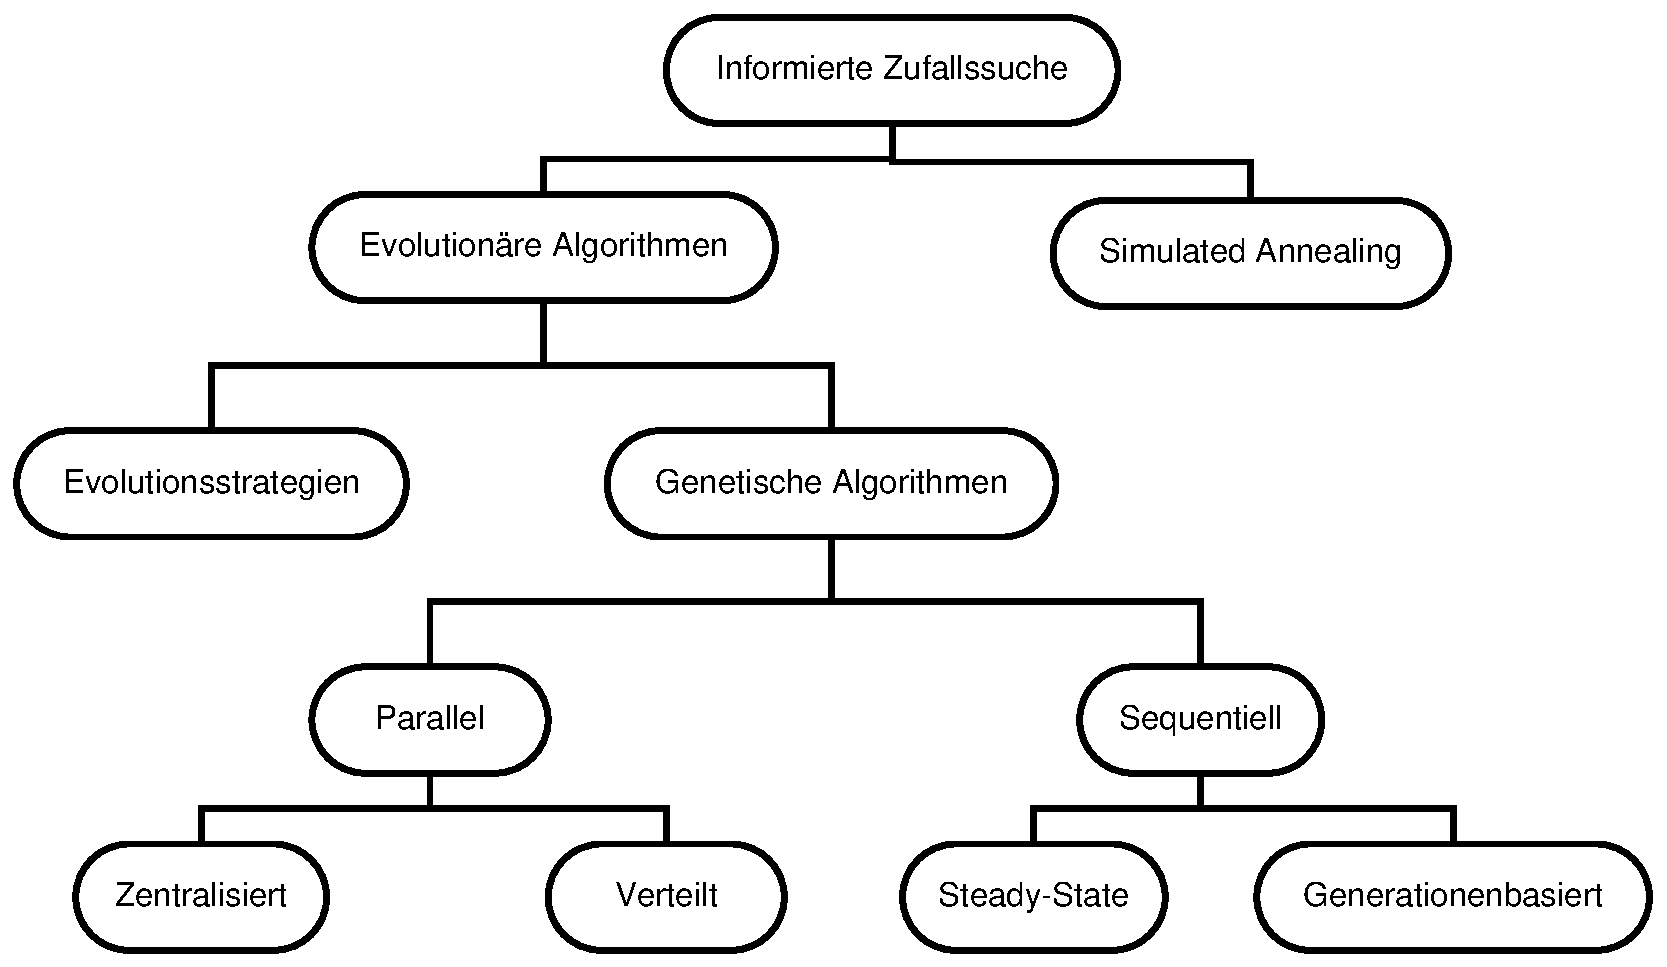
\includegraphics[scale=0.4]{unterteilung_EA_GA.eps}
\end{center}
\caption{Einteilung von Lernverfahren}
\label{genAbst}
\end{figure}


\subsubsection{Genetische Algorithmen (GA)}

Genetische Algorithmen k"onnen einfach beschrieben werden als: evolution"are Algorithmen + ``Crossover''

Vorbild: nat"urliche Evolution auf Genbasis

Dabei wird als ``Crossover'' der Vorgang bezeichnet, bei dem von zwei oder mehr Individuen die (Erb-)Informationen kombiniert werden, um ein neues Individuum zu schaffen.

\subsubsection{Klassische genetische Algorithmen (GA)}

Die klassischen genetische Algorithmen (GA) sind Algorithmen die auf einer Liste mit Bits arbeiten, welche die potentiellen Probleml"osungen/Individuen repr"asentieren. Mutation ist dabei das Invertieren von Bits. Beim Crossover gibt es meist one- oder two-point-crossover (bei GA's). Beim one-point-crossover wird die Bitsequenz der beiden Individuen jeweils an einem Punkt, meist die gleiche Position, durchgeschnitten und die beiden Teilh"alften eines Individuums mit den entsprechend anderen Teilh"alften des anderen Individuums verbunden. Two-point-Crossover ist identisch, nur das hier an zwei Punkten geschnitten wird.

%TODO
%Die Arbeitsweise von one-point-crossover ist in Bild \ref{onePCO} gezeigt, die von two-point-crossover im Bild \ref{twoPCO}  (beide "ubernommen aus \cite{GEA}).
%\begin{figure}[htbp]
%\begin{center}
%  \includegraphics[scale=0.5]{onePCO.jpg}
%\end{center}
%\caption{one-point-crossover}
%\label{onePCO}
%\end{figure}

%\begin{figure}[htbp]
%\begin{center}
%  \includegraphics[scale=0.5]{twoPCO.jpg}
%\end{center}
%\caption{two-point-crossover}
%\label{twoPCO}
%\end{figure}


\subsection{Anmerkungen zu evolution"aren Algorithmen (EA)}

Eine geeignete Wahl der Repr"asentation von L"osungen (also wie die Individuen aufgebaut sind) und angepasste Operatoren (welche die Individuen ver"andern bzw. neue Individuen erzeugen) k"onnen die Performance von evolution"are Algorithmen deutlich erh"ohen (\cite{ECDF00}).
Durch eine geeignete Wahl der Repr"asentation wird der Hypothesenraum, den diese aufspannen, g"unstig beeinflusst, z. B. k"onnen ung"ultige oder unerw"unschte L"osungen ganz entfallen. Weiterhin erm"oglicht eine gute Repr"asentation auch einen Hypothesenraum, in dem Operatoren einfacher zu realisieren sind, die im Allgemeinen schneller zur L"osung f"uhren, z. B. ist es dann wahrscheinlicher, dass "ahnliche L"osungen auch nahe im Hypothesenraum ``beieinanderliegen'' (f"ur die Operatoren).

Durch angepasste Operatoren werden die ``Wege'' (welche diese Operatoren im Hypothesenraum erzeugen) besser, bzw. f"uhren schneller zu besseren L"osungen. Es k"onnen beispielsweise als Operatoren schon bekannte Algorithmen zur Optimierung eingesetzt werden oder es kann in den Operatoren Wissen "uber das Problem verwendet werden.

Die gro"se Freiheit bei der Wahl der Repr"asentation der potentiellen Probleml"osung ist einer der gr"o"sten Vorteile der evolution"aren Algorithmen. Theoretisch ist eine beliebige Repr"asentation w"ahlbar, solange eine Bewertung von potentiellen Probleml"osungen in dieser m"oglich ist. Andere Lernverfahren erm"oglichen meist nur bestimmte Repr"asentationen, z. B. k"onnen Lernverfahren von neuronalen Netzen nur neuronale Netze als Probleml"osung hervorbringen. Bei EAs allerdings k"onnen unter anderen Bitlisten, Molek"ule, beliebige Programmiersprachen oder mathematische Formeln verwendet werden. Genauso variabel sind damit auch die Operatoren, mit denen die potentiellen L"osungen angepasst werden k"onnen. Damit k"onnen viel besser Vorwissen oder auch Vermutungen in den Algorithmus eingearbeitet werden.

Weiterhin kann bei der Wahl der Repr"asentation auch noch die Anschaulichkeit f"ur den Menschen ber"ucksichtigt werden. Das hei"st, die Repr"asentation kann so gew"ahlt werden, dass potentielle Probleml"osungen einfacher verstanden werden k"onnen.

Der gro"se Nachteil von evolution"aren Algorithmen ist der hohe Zeitaufwand bzw. Rechenaufwand den sie im Verh"altnis zu anderen Algorithmen ben"otigen. Wo andere Algorithmen die vorhanden Daten nutzen, um aus ihnen einmal eine L"osung zu generieren, generiert ein genetischer Algorithmus st"andig neue L"osungen, testet, wie gut diese sind, und w"ahlt m"oglichst die Guten aus. Solange die Terminalkondition nicht erf"ullt ist, h"alt ein genetischer Algorithmus auch nicht an. Die Terminalkondition kann aber auch sehr schwer oder gar nicht erf"ullbar sein. Ein gutes Beispiel ist auch hier die nat"urliche Evolution: Sie l"auft schon seit mindestens 4 Milliarden Jahren auf wenigstens einen ganzen Planeten, und es ist noch kein Ende abzusehen.


\section{Multimediaformate}

Multimedia ist der Begriff f"ur Informationen, wenn mehrere Medien geb"undelt werden. Medien sind Tr"ager von Dingen, die "uber Sinne wahrnehmbar sind, wobei den verschiedenen Sinnen jeweils ein Medium zugeordnet ist.
Multimediaformate sind danach S"atze von Regeln, wie diese Dinge abgespeichert (dauerhaft gemacht) oder "ubertragen werden k"onnen.

\bigskip\noindent
Dabei sind unter Anderem Medien f"ur folgende Dinge zu unterscheiden:
\begin{itemize}
\item Bild
\item Ton
\item olefaktorische Medien (Ger"uche)
\item hauptische Medien (wie sich ein Gegenstand anf"uhlt, z. B. hart oder rau)
\end{itemize}

Im Nachfolgenden werden vor Allem das Bild und der Ton beschrieben, da sie die gr"o"sten Bereiche sind (bzw. in unser heutigen Informationsgesellschaft am h"aufigsten anzutreffen sind).

\subsection{Bilder}

\subsubsection{Einleitung}

Wie auch in vielen anderen Bereichen wurde mit dem Aufkommen leistungsf"ahiger Computer die Bildverarbeitung revolutioniert. Handelte es sich Anfang der 60er Jahre \cite{projBildf}, als die grafische Datenverarbeitung aufkam, noch haupts"achlich um Strichzeichnungen und Diagramme, die erstellt, manipuliert und verarbeitet wurden, so sind es heutzutage ganze Filme, die mit Computern erzeugt werden. Es ist schon heute so gut wie unm"oglich, ein durch gute Manipulationen erstelltes Bild von einem ``echten'' (nicht manipuliertem) Bild zu unterscheiden.
Heute stehen eine Unzahl von Programmen zur Erstellung, Manipulation und Verarbeitung von Bildern zur Verf"ugung und damit einhergehend eine Unzahl von Bildformaten. Alle diese Bildformate haben ihre Vor- und Nachteile und werden in den verschiedensten Bereichen genutzt.

Im Nachfolgenden sollen einige wichtige Eigenschaften von Bildkodierungen n"aher erl"autert werden.

\subsubsection{Bildformat}

Ein Bildformat oder Bildkodierung ist ein Format (bzw. eine Strukturbeschreibung) f"ur eine Ansammlung von Daten, die ein Bild repr"asentieren. Dabei kommt es vor Allem auf die effiziente Organisation der Daten in Bezug auf das Anwendungsgebiet an. Die meisten Bildformate teilen ihre Daten in zwei Bl"ocke auf: einen Block mit allgemeinen Informationen zum Bild (Farbpalette, Bildgr"o"se, etc.) und einen Block der angibt, was auf dem Bild dargestellt wird (z. B. die Objekte oder die Farbwerte f"ur die einzelnen Pixel).
In Bild \ref{DatBit} ist als Beispiel der Aufbau einer Datei im Bitmapformat BMP (*.bmp) angegeben. Eingeleitet wird dieses Format durch den Bitmap Header, der anzeigt, dass es sich um ein Bitmapbild handelt (er besteht aus den Buchstaben ``bmp''). Im Informations-Header befinden sich Informationen zum Bild selbst, unter anderem sind dort zu finden: die H"ohe und Breite des Bildes, die horizontale und vertikale Aufl"osung in Pixel pro Meter, der Typ der Komprimierung und die Anzahl der benutzten Farben.

Die Farbpalette definiert jede Farbe durch ihren Anteil an Rot, Gr"un und Blau.
Die Daten enthalten die zeilenweise Rasterinformation des Bildes. Hierbei ist der
Ausgangspunkt die linke untere Ecke des Bildes.

\begin{figure}[htbp]
\begin{center}
\begin{picture}(5,4.5)
	\linethickness{4pt}
	\put(0,3){\framebox(4,1){Bitmap Header}}
	\put(0,2){\framebox(4,1){Informations-Header}}
	\put(0,1){\framebox(4,1){Farbpalette}}
	\put(0,0){\framebox(4,1){Daten}}
\end{picture}
\end{center}
\caption{Dateiaufbau eines Bitmap-Bildes}
\label{DatBit}
\end{figure}


\subsubsection{Eigenschaften von Bildern}

Wichtige Eigenschaften f"ur Bildformate werden im Folgendem aufgef"uhrt. Dabei m"ussen nicht alle Bildformate alle Eigenschaften unterst"utzen.

Der \textbf{Dateityp} (Filetype) ist das, woran im Dateisystem erkannt werden kann (oder zumindest erkannt werden sollte), um welche Art von Bildkodierung es sich handelt. Meist handelt es sich dabei um ein Dateiendungsk"urzel, das eine Art Abk"urzung der vollen Bezeichnung der Bildkodierungsart ist, z. B. die Dateiendung ``.bmp'' f"ur die Bitmap-Kodierung.

\bigskip\noindent
Die \textbf{maximale Bildgr"o"se} gibt an, wie die maximale Gr"o"se eines Bildes sein darf, um in diesem Bildformat noch abspeicherbar zu sein. Typisch ist hier die maximale Anzahl der Pixel, die ein Bild haben darf.
Die maximale Bildgr"o"se h"angt vom Speicherformat ab. Da in digitalen Rechnern nicht unendlich gro"se Zahlen abgespeichert werden k"onnen (wegen des begrenzten Speicherplatzes), k"onnen auch die Zahlen f"ur Koordinaten oder Bildgr"o"se nur endlich sein.

\bigskip\noindent
Die \textbf{Anzahl der Kan"ale} gibt an, aus wie vielen Teilbildern "ubereinander das Bild besteht. "Ublich ist ein Kanal, aber in einigen Anwendungen ist es notwendig, mehrere Bilder "ubereinander zu legen, um z. B. besser Transparenzen im Bild darstellen zu k"onnen.

\bigskip\noindent
Mit dem \textbf{Farbmodell} werden die Farben angegeben, die verwendet werden k"onnen. Der einfachste Fall ist z. B. S/W (nur schwarz und wei"s als ``Farben'').

\bigskip\noindent
Die \textbf{Farbtiefe} geh"ort zum Farbmodell und ist die Anzahl m"oglichen Farben, die einem Pixel oder Objekt zugeordnet werden k"onnen.
Farbtiefe in Bits ist die Anzahl der Bits pro Farbe, die einem Pixel oder Objekt f"ur dessen Farbe zugeordnet werden.
Die beiden Begriffe h"angen eng zusammen, da die Bits pro Farbe meist die Farbtiefe bestimmen nach der Formel: $Farbtiefe = 2 ^ {(Bits\ pro\ Farbe)}$

\bigskip\noindent
Der \textbf{Hersteller} eines Bildformates ist wichtig im Hinblick auf Lizenzen und m"ogliche Updates. Muss f"ur ein Bildformat bezahlt werden, wenn es in einer Software benutzt werden soll? Wird dieses Bildformat in Zukunft eventuell noch besser ausgebaut usw. ?

\bigskip\noindent
\textbf{Plattformabh"angigkeit}: Bei vielen unbekannteren Bildformaten gibt es nur f"ur einige Plattformen (z. B. Rechnertypen oder Betriebsysteme) Programme zum Erstellen, Bearbeiten oder Darstellen von Bildern in ihnen.

\bigskip\noindent
Als \textbf{Komprimierung} wird bezeichnet, wie viel Informationen (Bits) f"ur ein Bild ben"otigt werden, um es aus diesen wiederherzustellen.

\bigskip\noindent
Die \textbf{Darstellungsarten} Vektorgrafik oder Rastergrafik beziehen sich auf die Art, wie die Bildinformationen abgespeichert sind. Bei Rastergrafiken wird "uber das Bild ein Raster gelegt und die einzelnen Punkte abgespeichert. Bei Vektorgrafik werden die ``Objekte'' (z. B. Linien, Kreise) des Bildes abgespeichert.


\subsubsection{Kodierungen in den Darstellungsarten Vektorgrafik oder Rastergrafik}

\paragraph{Vektorgrafik:}

Bei der Vektorgrafik werden die Daten f"ur einzelne Objekte (dessen ``Vektoren'') gespeichert. Der Vektorgrafiktyp bestimmt die m"oglichen Objekte. Oft finden daf"ur Punkte, Linien und Kreise Verwendung. Der Vektorgrafiktyp, und damit die verwendeten Objekte, orientieren sich meist stark an dem Anwendungsgebiet, f"ur das dieser Vektorgrafiktyp geschaffen wurde, z. B. technischer Entwurf von Geb"auden oder Ger"aten. Die Objekte werden mathematisch durch eine Anzahl von Werten definiert, z. B. Anfangsposition, L"ange oder Radius. Vektorgrafiken sind vor allem bei technischen Zeichnungen verbreitet (z. B. CAD-Systeme).

\bigskip\noindent
Vorteile:
\begin{itemize}
  \item Grafikobjekte k"onnen (meist) ohne Qualit"atsverlust verschoben, skaliert oder mit Farbe versehen werden.
  \item Ein Vektorbild besteht aus vielen verschiedenen Einzelobjekten, die sich bei Ver"anderungen gegenseitig nicht beeinflussen.
  \item Im Vergleich zu Rastergrafiken wird hier meist weniger Speicherplatz ben"otigt, da eine geringere Anzahl von Informationen gespeichert wird (z. B. einen Kreis als Matrix/Raster aus Farbwerten zu beschreiben, wie bei der Rastergrafik, ist aufwendiger, als einen Kreis mit Mittelpunkt und Radius zu beschreiben).
  \item Die Vektorgrafiken sind (meist) nicht an eine bestimmte Aufl"osung gebunden, d. h. sie passen sich den M"oglichkeiten des Ausgabeger"ats an.
\end{itemize}


\bigskip\noindent
Nachteile:
\begin{itemize}
  \item	Zur Bildschirm- und Druckerausgabe m"ussen die Vektorgrafiken gerastert werden, da diese Ger"ate nur Punkte darstellen k"onnen. Ein Treppeneffekt ist die Folge.
  \item	Eine direkte Umwandlung von Rastergrafik oder Vektorgrafiken eines Typs in eine Vektorgrafik anderen Typs ist meist nur schwer und mit viel Aufwand zu realisieren. (Bei Vektorgrafiken geht es darum, die Objekte des Bildes darzustellen. Wie findet man aber solche bei Rastergrafiken? Einfach jeden Punkt als Objekt [z. B. als Rechteck] zu deklarieren, w"urde keinen der oben genannten Vorteile bringen.)
  \item	Die meisten Bilder liegen nach dem Einlesen in einem Rastergrafikformat vor.
\end{itemize}


\paragraph{Rastergrafik:}

Bei der Rastergrafik (auch Bitmapgrafik) wird "uber das Bild ein Raster gelegt und die einzelnen Punkte bzw. ihre Farbe (im Farbmodell) abgespeichert. Damit besteht ein Rasterbild aus einer Menge von Pixeln (Bildpunkten), die eine bestimmte Farbe haben. Bei gen"ugend vielen Pixeln pro Fl"ache und gen"ugend Farben kann das menschliche Auge die einzelnen Pixel nicht mehr wahrnehmen und es entsteht der Effekt eines ``fotorealistischen'' Bildes.

\bigskip\noindent
Vorteile:
\begin{itemize}
  \item	einfaches Abspeichern von Bildern, es m"ussen keine Objekte bekannt sein
  \item	Da die meisten Ger"ate (z. B. Monitor, Scanner, Drucker) zum Darstellen oder Einlesen von Bildern mit Rastern arbeiten, ist die Umwandlung in oder von Rastergrafiken f"ur diese Ger"ate einfach.
\end{itemize}

\bigskip\noindent
Nachteile:
\begin{itemize}
  \item	Da jeder einzelne Punkt eines Bildes abgespeichert wird, kostet es meist viel Speicherplatz.
  \item	Bei einer starker Vergr"o"serung eines Rastergrafikbildes kommen die einzelnen Pixel zum Vorschein und die Grafik wirkt eckig.
  \item	Objekte des Bildes k"onnen nur noch schwer oder gar nicht automatisch identifiziert werden.
\end{itemize}

\subsubsection{Farbmodell/Farbschema}

Das Farbmodell gibt an, wie die Farben im Bild dargestellt werden. Es handelt sich bei diesen Farben um einen Vektor mit diskreten (z. B. ganzen) Zahlen aus einem Definitionsbereich. Dieser Vektor wird dann jeweils einem Pixel oder einem anderem Objekt (bei Vektorgrafik) zugeordnet. Der Darstellbarkeit wegen werden Schwarz und Wei"s auch als Farben angesehen. Ihnen ist im allgemeinen auch ein Vektor zugeordnet.
Die Anzahl der Farben, die ein Bild haben kann, wirkt sich stark auf die Gr"o"se des n"otigen Speichers f"ur dieses aus.

\bigskip\noindent
Im Nachfolgenden sind einige bekannte Beispiele aufgef"uhrt.

\paragraph{S/W (schwarz/wei"s):}

Das S/W-Farbmodell (S/W steht dabei f"ur schwarz/wei"s) ist wohl das "alteste, einfachste und am wenigsten speicheraufw"andige Farbmodell. Dabei wird pro Objekt (z. B. pro Pixel) ein Bit gespeichert, das je nach Wert (z. B. wei"s = true, schwarz = false) angibt, ob das Objekt (z. B. der Punkt) wei"s oder schwarz sein soll bzw. heller oder dunkler darzustellen ist, z. B. f"ur Monitore die kein wirkliches Schwarz oder Wei"s darstellen k"onnen.


\paragraph{Grayscale (Halbton):}

Beim Grayscale werden 256 Abstufungen von schwarz bis wei"s unterschieden. Pro Objekt werden daf"ur ein Byte oder acht Bit abgespeichert. Dies wird dann als eine dieser Abstufungen interpretiert.


\paragraph{RGB:}

Das RGB-Farbmodell ist ein additives Verfahren, mit den drei Grundfarben Rot, Gr"un und Blau. Jeder dieser Grundfarben ist ein Wert zugeordnet: Umso gr"o"ser dieser ist, desto heller ist der entsprechende Anteil dieser Grundfarbe in der erzeugten Farbe. %, dargestellt in Bild \ref{RGB} ("ubernommen aus \cite{projBildf}). 
Mit diesem Farbmodell k"onnen alle Farben mit einer Genauigkeit dargestellt werden, die mit der Definitionsbereichsgr"o"se der einzelnen Farben ansteigt.
Das Farbmodell hat seinen Ursprung in der Realisierung von Farben auf Monitoren (Braunsche R"ohren), da auch dort nur drei verschiedenfarbige Punkte zu einem Pixel zusammenfasst werden: Je st"arker der Elektronenstrahl einen dieser Punkte anstrahlt, desto heller erscheint er in seiner Farbe. Daher eignet sich dieses Farbmodell auch besonders gut f"ur diese Monitordarstellungen, es muss nicht mehr viel umgerechnet werden.

%TODO
%\begin{figure}[htbp]
%\begin{center}
%  \includegraphics[scale=0.5]{RGBFarb.jpg}
%\end{center}
%\caption{additives Farbschema}
%\label{RGB}
%\end{figure}
 
\paragraph{Indizierte Farben:}

Bei indizierten Farben wird nicht immer der gleiche ``Farb\-raum'' f"ur jedes Bild verwandt, sondern je nach Bild, je nach dem welche Farben bei ihm ben"otigt werden, nur diese Farben oder "ahnliche. Jede dieser Farben bekommt eine ``Nummer'' (Indices), die in einer Tabelle der wirklichen Farbe (z. B. im RGB-Farbmodell) zugeordnet wird. Da im Bild nun viel weniger Farben dargestellt werden m"ussen, wird Speicherplatz gespart. 

\subsubsection{Komprimierung}

Bei der Komprimierung geht es darum, Speicherplatz f"ur ein Bild zu sparen. Umso weniger Speicherplatz ein Speicherformat f"ur ein Bild ben"otigt, desto h"oher wird der Kompressionsfaktor dieses Speicherformats angesehen. Ein h"oherer Kompressionsfaktor eines Speicherformats f"uhrt meist zu einen h"oheren Kompressionsfaktor eines in ihm abgespeicherten Bildes. Leider ist die Festlegung, f"ur welches Speicherformat der Kompressionsfaktor null ist, mehr oder weniger willk"urlich, denn es k"onnen immer zu einem Speicherformat weitere Informationen "uber das abgespeicherte Bild hinzugef"ugt (z. B. Redundanzen, History) und der Kompressionsfaktor verschlechtert werden.
Der Ausdruck ein Bild sei ``unkomprimiert'' ist somit nicht zutreffend. Zutreffender ist, dass solche Bilder einen niedrigen Kompressionsgrad haben.

\bigskip\noindent
Es werden zwei gro"se Komprimierungsarten unterschieden.

\paragraph{Verlustfreie Komprimierung:}

Dabei gehen keine Informationen "uber das Bild verloren. Das hei"st, wenn ein Bild mit einem verlustfreien Verfahren komprimiert und danach wieder hergestellt wird, ist das Abbild mit dem Original identisch.

\paragraph{Verlustbehaftete Komprimierung:}

Dabei gehen Informationen "uber das Bild verloren. Das hei"st, wenn ein Bild mit einem verlustbehafteten Verfahren komprimiert und danach wieder hergestellt wird, ist das Abbild mit dem Original nicht mehr identisch. Es k"onnen z. B. Pixel mit einer leicht abweichenden Farbe im Abbild vorhanden sein.

In dieser Komprimierungsart sind meist h"ohere Komprimierungsfaktoren m"oglich als mit der verlustfreie Komprimierung.


\subsection{Ton}

T"one sind Schwingungen. Die Schwingung kann dabei durch unterschiedliche Medien (z. B. Luft oder Wasser) "ubertragen werden. T"one setzen sich aus elementaren Schwingungen mit unterschiedlichen Frequenzen, Amplituden, Anfangszeitpunkten und Dauer zusammen.

Deutlich wird dies beispielsweise beim Klavierspielen. Wenn ein Klavierst"uck gespielt wird, werden die Tasten des Klaviers zu einer bestimmten Zeit gedr"uckt, woraufhin ein Ton einer bestimmten L"ange erklingt. Dieser Ton ist aus unterschiedlichen Frequenzen zusammengesetzt und hat eine bestimmte Lautst"arke, welche durch die Amplituden der Frequenzen bestimmt wird.

\bigskip\noindent
T"one k"onnen demnach abgespeichert werden indem die Schwingungen des Tons aufgezeichnet werden oder die Frequenzen.

Werden die Schwingungen des Tons aufgezeichnet (wie z. B. beim wav-Format), h"angt die Quallit"at von der Dichte der Aufzeichnungspunkte ab. F"ur jeden Aufzeichnungspunkt wird die Amplitude gespeichert. Werte von 44000 Aufzeichnungspunkten pro Sekunden sorgen f"ur einen Ton in einer guten Qualit"at. Da pro Aufzeichnungspunkt ein paar Bytes (f"ur die Amplitude) verbraucht werden, ist der Speicherbedarf relativ hoch (allein bei $2$ Bytes f"ur die Amplitude $44000 \frac{1}{s} * 2 Byte = 88000 Byte/s$, bei einer Aufzeichnung von nur 3 Minuten sind das rund 15,1 MB). Dieser Speicherbedarf verdoppelt sich noch, wenn die Aufzeichnung in Stereo gemacht werden soll.

Mit dem Abspeichern der Frequenzen von T"onen k"onnen im Allgemeinen bessere Komprimierungsraten erreicht werden. Diese kann noch gesteigert werden, wenn Frequenzen, die der Mensch normalerweise nicht wahrnimmt, nicht mit abgespeichert werden (wie z. B. beim MPEG-Audio [z. B. mp3]). Diese Art des Abspeicherns ist aber auch rechenaufw"andiger.


%TODO
%\section{Weitere Medien}
%\subsection{Olifaktorische Medien}
%\subsection{Hauptische Medien}




%TODO
%
% Copyright (c) 2008  Betti "Osterholz
%
% Permission is granted to copy, distribute and/or modify this document
% under the terms of the GNU Free Documentation License, Version 1.2 or
% any later version published by the Free Software Foundation;
% with no Invariant Sections, no Front-Cover Texts, and no Back-Cover Texts.
%
% A copy of the license is included in the file ``fdl.tex'' .
%

%path for pictures
\graphicspath{{./material_sprachbeschreibung/}}
\graphicspath{{./material_sprachbeschreibung/}{../material_sprachbeschreibung}}


\newpage
\part{Fib-Sprachbeschreibung}
\label{partFibLanguage}

In diesem Teil werden die Elemente der Fib-Multimediasprache vorgestellt und einige grundlegende Aussagen zur Fib-Multimediasprache getroffen.


\section{Anforderungen}
\label{secFibLanguageRequirements}

Da die klassische Bitdarstellung bei genetischen Algorithmen eine geringe Performance erwarten l"asst,  aber gerade wegen der Komplexit"at des Problems eine m"oglichst hohe Performance von N"oten ist, wird eine angepasste Problemdarstellung (Multimediabeschreibungssprache) gew"ahlt.

Die Multimediabeschreibungssprache Fib sollte m"oglichst einfach gehalten werden, mit m"oglichst wenigen Alternativen, da mit dem Anstieg der zur Auswahl stehenden Alternativen auch die Anzahl der Alternativen bei der Anwendung der genetischen Operationen steigt und damit wahrscheinlich der Rechenaufwand und der Realisierungsaufwand.

Dennoch sollen mit der Multimediabeschreibungssprache kompakte Ausdr"ucke f"ur ``normale'' (in der Anwendung auftretende) Multimediaobjekte m"oglich sein. Es soll also gute Komprimierungsm"oglichkeiten f"ur ``normale'' Multimediaobjekte geben. Das beinhaltet, dass Zusammenh"ange (z. B. Farbverl"aufe in einer Fl"ache) zwischen Teilen (z. B. Pixeln der Fl"ache) eines Multimediaobjekts m"oglichst einfach dargestellt werden k"onnen.

Die Sprache sollte eindeutig, reproduzierbar und auswertbar sein, so dass ein Ausdruck immer zum gleichen Objekt ausgewertet wird. Bei der Eindeutigkeit und Reproduzierbarkeit k"onnen in der Implementierung Abstriche gemacht werden (z. B. wegen unterschiedlichen Rundungsfehlern auf unterschiedlichen Architekturen), wenn das erzeugte Multimediaobjekt so gut wie immer (in beispielsweise dem 0,999999sten Anteil der F"alle) dem original Multimediaobjekt sehr "ahnlich ist. Die g"ultigen Sprachobjekte m"ussen jedoch immer auswertbar sein, da sonst Einschr"ankungen bei den genetischen Operatoren, die sie erzeugen, gemacht werden m"ussten oder nicht auswertbare Objekte entstehen k"onnten.

Es soll mit der Multimediabeschreibungssprache m"oglich sein, zumindest alle m"oglichen Rastergrafiken darzustellen.
Die Erzeugung einer Rastergrafik aus einem Fib-Multimediaobjekt in der Multimediabeschreibungssprache soll nachvollziehbar sein. Das hei"st, die Multimediabeschreibungssprache soll die Unterscheidung einzelner Objekte und deren Zusammenhang unterst"utzen.

Die Multimediaprogramme ver"andernden genetischen Operationen sollten, wenn m"oglich, das Programm so ver"andern, dass im Hypothesenraum der Multimediaprogramme diese Operatoren einen Gradientenanstieg erm"oglichen. Durch Ausf"uhrung mehrerer Operatoren sollte also die Hypothese, die das Multimediaprogramm darstellt, allm"ahlich verbessert werden k"onnen.


\section{Die Multimediabeschreibungssprache}

Die Multimediabeschreibungssprache tr"agt den Namen Fib (f"ur funktionale Interpretation von Bildern oder ``functional interpretation of bictures/bitmaps''). Dieser Namen leitet sich noch aus der ersten Version der Multimediabeschreibungssprache her, als sie nur zum Abspeichern von Bildern geeignet war.

Durch einige zus"atzliche Elemente wurde die Multimediabeschreibungssprache so erweitert, dass sie beliebige Multimediadaten abspeichern kann. Die einzige Einschr"ankung bez"uglich der Multimediadaten ist, dass sie als Eigenschaften von Punkten eines endlichen, euklidischen und diskreten (es gibt kleinste Einheiten) Raumes darstellbar sind.

Fib ist eine Vektordarstellung von Multimediadaten, also eine Darstellung von Multimediadaten mit Hilfe von Objekten.
Als Grundger"ust dient ein Baum. Die Bl"atter sind Endpunkte, die f"ur die Darstellung von bzw. Zuordnung zu Punkten oder Teilmultimediaobjekten dienen. In den "Asten und der Ausrichtung dieser, welche z. B. am weitesten links stehen, werden Darstellungsparameter oder Eigenschaften der Bl"atter kodiert, z. B. wie oft es dargestellt wird und mit welcher Farbe.

Jeder Knoten des Baums ist ein Fib-Element. Der Baum wird von der Wurzel zu den Bl"attern ausgewertet, wobei die Elemente die Auswertung beeinflussen.

Ein vollst"andiges Fib-Objekt (Baum) repr"asentiert ein Multimediaobjekt.

Ein g"ultiges Fib-Objekt (Baum) ist zyklenfrei, um eine endliche Verarbeitungszeit zu gew"ahrleisten.
Die Elemente der Multimediabeschreibungssprache orientieren sich dabei etwas an den "ublichen imperativen Programmiersprachen (z. B. C++, Java).

Alle Einheiten sind auf Grundlage des Internationalen Einheitensystems (SI) anzugeben.

Beim Auswerten eines Fib-Objekts werden f"ur das Multimediaobjekt alle Punkte mit ihren Eigenschaften ermittelt. Ein ausgewertetes Multimediaobjekt enth"alt damit nur eine Liste von konkreten Punkten und ihren Eigenschaften, so dass es direkt angezeigt (durch Darstellung der Eigenschaften an den Punkten/Koordinaten) bzw. ausgewertet werden kann.

Im Nachfolgenden wird als ``oben'' im Fib-Objekt die Richtung bezeichnet, in der die Wurzel des Baums liegt. Die Richtung ``unten'' ist damit die entgegengesetzte Richtung (also weg von der Wurzel).


\section{Elemente der Fib-Multimediabeschreibungssprache}
\label{secFibElements}

In diesem Abschnitt werden die Elemente beschrieben, aus denen die Fib-Multi\-media\-beschrei\-bungs\-sprache aufgebaut ist.

Im Nachfolgendem bezeichnet $Obj$ ein Fib-Objekt.



\subsection{Vektoren}\index{Vektoren|(}

Vektoren dienen zum Bereitstellen von numerischen Werten. Es gibt verschiedene Typen von Vektoren (z. B. Positionsvektor, Bereichsvektor oder Eigenschaftsvektor f"ur RGB-Farben). Aus dem Typ eines Vektors (und eventuell den Angaben im root-Element) ergeben sich die Anzahl und die Definitionsbereiche der Elemente, die er enthalten kann.
Jedes Vektorelemente ist entweder eine Zahl oder eine Variable, welche weiter oben im Fib-Objekt belegt wird.

Liegt der Werte eines ausgewerteten Elements au"serhalb des Definitionsbereichs, f"ur den das Vektorelement definiert ist, wird dieser Wert auf den n"achsten Wert gerundet, der im Definitionsbereich liegt.
Wenn ein Element des Vektors nicht belegt ist, wird es als der Nullwert des Definitionsbereichs ausgewertet.

Vektoren eines Typs k"onnen nur in einem ganz bestimmten Fib-Element verwendet werden.

Eine Auflistung der m"oglichen Vektoren ist in Tabelle \ref{tableVectorTyps} zu sehen.

\begin{table}[htbp]
\begin{center}
\begin{small}
\begin{tabular}{|p{20mm}|p{35mm}|p{15mm}|p{20mm}|p{15mm}|}\hline
	Vektor & Beschreibung & wird verwendet in Fib-Element & Anzahl Elemente & Typ Elemente \\\hline\hline
	Position & gibt die Position eines Punktes an & $point$ (Punkt) & beliebig (Vektor mit 0 Elementen ist immer m"oglich) & Zahlen\\\hline
	Bereich & gibt die Grenzen eines Teilbereichs (inklusive der Grenzen) an & $area$ (Bereich) & 2 & ganze Zahlen\\\hline
	Eigenschafs\-vektoren (es kann beliebige geben) & definiert die Werte einer Eigenschaft & $property$ (Eigenschaften) & beliebig & Zahlen\\\hline
\end{tabular}
\end{small}
\end{center}
\caption{Vektorentypen}
\label{tableVectorTyps}
\end{table}

\index{Vektoren|)}


\subsection{Punkte}\index{Punktelement|(}
\label{fibPoint}\label{secFibPoint}

\begin{flushleft}
Die Punkte sind die darstellenden Elemente. An ihnen werden die gesetzten Eigenschaften ausgewertet. Punkte dienen als Bl"atter eines Fib-Objekts.

Ein leerer Punkte ``point()'' ist m"oglich. Der leere Punkt hat keine Auswirkungen (alle Eigenschaften gehen verloren). Genutzt werden kann er in Kombination mit anderen Elementen (z. B. dem $if$-Element).

Daneben gibt es auch Punkte mit leerem Positionsvektor ``point(())'', diese erzeugen den Hintergrund (z. B. Hintergrundfarbe).

Die Eigenschaften des Punkts (z. B. Farbe, Ton oder/und Geruch) werden im Ast "uber dem Punkt durch property-Elemente bestimmt.

\bigskip\noindent
Syntax:
$Obj = point( PositionVector )$

\bigskip\noindent
Kurzsyntax:
$Obj = p( PositionVector )$

\bigskip\noindent
Beschreibung der Elemente:
\begin{description}
 \item[$PositionVector$]: die Koordinatenvektor des Punktes
\end{description}

\bigskip\noindent
Beispiel:
\begin{itemize}
 \item $p((10;20))$; Ein Punkt an der Position $(10, 20)$.
 \item $p((10;x))$; Das Symbol $x$ steht f"ur eine Variable, die im Ast zu diesem Punkt belegt werden muss.
 \item $p()$; Der Punkt hat keine Auswirkungen und alle Eigenschaften werden verworfen.
 \item $p(())$; Der Punkt wirkt sich auf den gesamten Hintergrund aus.
\end{itemize}

\end{flushleft}

\index{Punktelement|)}


\subsection{Eigenschaftselement}\index{Eigenschaftselement|(}
\label{fibProperty}\label{secFibProperty}

Mit dem Eigenschaftselement ``property'' werden Eigenschaften f"ur Fib-Objekte gesetzt.

\bigskip\noindent
Syntax:
$Obj = property( ( value_1, ..., value_n)_{name}, Obj_1 ) $

\bigskip\noindent
Kurzsyntax:
$Obj = pr( (value_1, ..., value_n)_{name}, Obj_1 )$

\bigskip\noindent
Beschreibung der Elemente:
\begin{description}
 \item[$name$] Der $name$ gibt den Namen der Eigenschaft an. Er bestimmt den Typ des Vektors. Alle Eigenschaftsvektortypen sollten zum Vektorobertyp ``property'' geh"oren.
 \item[$value_i$] Dies ist der Wert $i$ der Eigenschaft.
 \item[$Obj_1$] Das ist das enthaltende Objekt, f"ur welches die Eigenschaft gesetzt wird.
\end{description}


\begin{small}
\begin{center}
\begin{longtable}{|p{22mm}|p{6mm}|p{5mm}|p{50mm}|p{30mm}|}\hline
	\textbf{Name} & \textbf{Wert} & \textbf{\#El.} & \textbf{Beschreibung} & \textbf{Beispiel} \\\hline\endhead
	whatever & 0 & 0 & Die Eigenschaften des Unterobjekts ist egal. Welche Eigenschaften diesem Unterobjekt auch immer zugeordnet werden, sie sind richtig. & pr( $()_{whatever}$, Obj )\\\hline
	\multicolumn{5}{|c|}{\textbf{Farben}}\\
	\multicolumn{5}{|c|}{(Alle Farben "uberschreiben die f"ur das aktuelle Fib-Objekt gesetzten Farben.)}\\\hline
	colorRGB & 1 & 3 & Farbanteile als Rot-, Gr"un- und Blau-Werte & pr( $(255, 16, 0$ $)_{colorRGB}$, Obj )\\\hline
%TODO?: colorCMYK
	colorGrayscale & 2 & 1 & Helligkeitsanteil & pr( $(25)_{colorGrayscale}$, Obj )\\\hline

	\multicolumn{5}{|c|}{\textbf{weitere Eigenschaften}}\\\hline
	layer & 100 & 1 & Ebenen f"ur die Punkte (niedrige Ebenen werden von h"oheren "uberdeckt) & pr( $(2)_{layer}$, Obj )\\\hline
	transparency & 200 & 1 & Durchsichtigkeitsanteil (f"ur Farben) der Punkte & pr( $(25)_{transparency}$, Obj ) \\\hline
	persistent & 210 & 0 & Diese Eigenschaft ist nur f"ur einen Zeitraum (bzw. der Dimensionsrichtung Zeit) sinnvoll. Raumpunkte mit diese Eigenschaft verlieren ihre anderen Eigenschaften nur, wenn diese zeitlich sp"ater durch jeweils eine Eigenschaft vom gleichen Typ "uberschrieben wird. Dies gilt nat"urlich nur, solange der jeweilige "uberschriebene Punkt die Eigenschaft $persistent$ hat. Sinnvoll ist dies, wenn beispielsweise in einem Film Objekte so lange sichbar sein sollen, wie sie nicht von anderen Objekten "uberschrieben werden. Dann kann das gesamte Fib-Objekt die Eigenschaft $persistent$ bekommen. Wird dann ein Objekt zu einer Zeit definiert und angezeigt, bleibt es in Zukunft solange bestehen, bis es "uberschrieben wird. &  pr( $()_{persistent}$, Obj ) \\\hline

	\multicolumn{5}{|c|}{\textbf{Ton-Eigenschaften}}\\\hline
	sound & 300 & 4 & ein Ton; Die Werte sind: 1. Frequenz in Hertz ($1/s$), 2. Schalldruck in Pascal $Pa$ ($1 Pa= 1 N/m^2$), 3. Phasenverschiebung in Bogenma"s 4. Dauer in Sekunden. Ein Ton wirkt additiv mit anderen T"onen. & pr( $(5000, 40, 0.5, 50$ $)_{sound}$, Obj) \\\hline
	soundPolarized & 301 & $3 + \sharp$ $Dim$ & ein Ton; Die Werte sind: 1. Frequenz in Hertz ($1/s$), 2. Schalldruck in Pascal $Pa$ ($1 Pa= 1 N/m^2$), 3. Phasenverschiebung in Bogenma"s, 4. Dauer in Sekunden, r = $5$ bis ($3 + \sharp Dim$) Polarisierungsanteil (als Winkel in Bogenma"s) in der Dimensionsebene, welche von den jeweiligen Dimensionen $r-4$ und $r-3$ aufgespannt wird. ($\sharp Dim$ ist die Anzahl der Dimensionen.) Die Winkelangabe erfolgt von der $r-3$ Achse in positiver Richtung. Ein Ton wirkt additiv mit anderen T"onen. & pr( $(5000, 40, 2, 0.5, 5$ $)_{soundPolarized}$, Obj) \\\hline

	soundAmplitude & 305 & 3 & die Amplitude eines Tons; Die Werte sind: 1. Schalldruck in Pascal $Pa$ ($1 Pa= 1 N/m^2$), 2. Phasenverschiebung in Bogenma"s 3. Dauer in Sekunden. Ein Ton wirkt additiv mit anderen T"onen. Mit dieser Eigenschaft k"onnen T"one "uber ihre Amplituden mit einer bestimmten Abtastrate aufgebaut werden, wie z. B. im WAVE-Dateiformat. & pr( $( 40, 0.5, 0.0005$ $)_{soundAmplitude}$, Obj) \\\hline

	soundBarrier & 310 & 1 & Geschwindigkeit des Schalls in Meter pro Sekunde ($m/s$); Damit k"onnen Objekte die Akustik ver"andern. & pr( $(343)_{soundBarrier}$, Obj) \\\hline
	soundReflected & 311 & 1 & Anteil des vom Objekt zur"uckgeworfener Schalls; Diese Eigenschaft gilt f"ur die Oberfl"ache/den Rand des Objekts und nicht f"ur alle seine einzelnen Punkte. & pr( $(50)_{soundReflected}$, Obj) \\\hline
	soundDamping & 312 & 1 & Anteil des von einem Punkt geschluckten Schalls & pr( $(2)_{soundDamping}$, Obj) \\\hline

	\multicolumn{5}{|c|}{\textbf{Physikalische Eigenschaften}}\\\hline
	kelvin & 400 & 1 & Temperatur in Kelvin & pr( $(300)_{kelvin}$, Obj) \\\hline
%TODO: Beschleunigungsfeld (Gavitation); Elektrischesfeld, Magnetischesfeld

%TODO: weitere Eigenschaften: Richtung, Strahlenkegel ...
	electroMagnetic  & 410 & $3 + \sharp$ $Dim$ & eine elektromagnetische Strahlungsquelle; Die Werte sind: 1. Frequenz in Hertz ($1/s$), 2. Amplitude in Candela cd, 3. Phasenverschiebung in Bogenma"s, 4. Dauer in Sekunden, r = $5$ bis ($3 + \sharp Dim$),  r = $5$ bis ($3 + \sharp Dim$) Polarisierungsanteil (als Winkel in Bogenma"s) in der Dimensionsebene, welche von den jeweiligen Dimensionen $r-4$ und $r-3$ aufgespannt wird ($\sharp Dim$ ist die Anzahl der Dimensionen). Die Winkelangabe erfolgt von der $r-3$ Achse in positiver Richtung. Ein elektromagnetische Welle wirkt additiv mit anderen elektromagnetische Wellen. & pr( $(5{,}3* 10^{14}, 2, 0.5, 0.5, 50$ $)_{electroMagnetic}$, Obj) \\\hline

%TODO: atom( Anteil in Mischung, Anzahl Proton, difference Elektronen to Protonen, difference Neutronen to Protonen )


	\multicolumn{5}{|c|}{\textbf{Objektbeschreibende Eigenschaften}}\\
	\multicolumn{5}{|c|}{(Diese beschreiben nur die Teilobjekte ohne weitere Auswirkungen.)}\\\hline
	periodBegin & 500 & 1 & Zeit in Sekunden ($s$) ab dem Anfang des Gesamt-Multimediaobjekts, ab dem das Objekt dargestellt werden soll. Diese Eigenschaft sollte m"oglichst nahe an der Wurzel des Multimediaobjekt stehen. Mit der Eigenschaft kann beim Abspielen eines Multimediaobjekts bestimmt werden: in welcher Reihenfolge Teilobjekte auszuwerten sind oder/und bis wann ein Teilobjekt auszuwerten ist. & pr( $(0.3)_{periodBegin}$, Obj) \\\hline
	periodEnd & 501 & 1 & Zeit in Sekunden ($s$) ab dem Anfang des Gesamt-Multimediaobjekts, bis zu dem das Objekt dargestellt werden soll. Diese Eigenschaft sollte m"oglichst nahe an der Wurzel des Multimediaobjekts stehen und einer ``periodBegin''-Eigenschaft folgen. Mit der Eigenschaft kann beim Abspielen eines Multimediaobjekts bestimmt werden: in welcher Reihenfolge Teilobjekte auszuwerten sind oder/und bis wann ein Teilobjekt vollst"andig auszuwerten ist. & pr( $(0.4)_{periodEnd}$, Obj) \\\hline
	evaluationTime & 502 & 1 & Zeit die zum Auswerten eines Multimediaobjekts ben"otigt wird, bezogen auf ein Multimediaobjekt, welches nur einen Punkt enth"alt (die Angabe ist als vielfaches der Auswertungszeit f"ur einen Punkt zu sehen). Mit dieser Eigenschaft kann zusammen mit den Eigenschaften ``periodBegin'' und ``periodEnd'' beim Abspielen eines Multimediaobjekts eine sinnvolle Auswertungsreihenfolge und die sinnvollen Auswertungszeitpunkte der Teilobjekte bestimmt werden. Diese Eigenschaft sollte direkt nach (bzw. unterhalb /innerhalb) ``periodBegin'' und ``periodEnd'' stehen. & pr( $(0.15)_{evaluationTime}$, Obj) \\\hline

	\multicolumn{5}{|c|}{\textbf{Eigenschaften f"ur das komprimierte Abspeichern}}\\
	\multicolumn{5}{|c|}{(Diese haben keine Auswirkungen auf die Punkte.)}\\\hline
	checksum & 600 & 3 & Es wird eine Checksumme f"ur das Objekt generiert. Dabei gibt der erste Parameter die Art der Checksumme an. Der zweite Parameter gibt an, alle wieviel Bits eine Check\-summe generiert werden soll, und der dritte Parameter, wieviel Bits die Checksumme haben soll. Der letzte Block der Checksummenbl"ocke wird nach dem Laden mit 0 aufgef"ullt, so dass auch er die gew"unschte L"ange hat. Sind genug Bits zur Korrektur eines Fehlers vorhanden, wird eine Korrektur eines Fehlers beim Laden versucht (siehe Abschnitt \ref{secCompressedChecksumm} auf Seite \pageref{secCompressedChecksumm}). & pr( $( 1, 1024, 16$ $)_{checksum}$, Obj )\\\hline
	boundSize & 601 & 0 & F"ur das enthaltende Objekt wird beim komprimierten Abspeichern die Grenze/Gr"o"se in Bits vermerkt. Wenn beim Laden dann ein Fehler im Fib-Objekt auftritt, k"onnen die nachfolgenden Fib-Elemente immer noch geladen werden, da deren Anfang bekannt ist (siehe Abschnitt \ref{secCompressedBoundSize} auf Seite \pageref{secCompressedBoundSize}). & pr( $()_{boundSize}$, Obj )\\\hline

	\multicolumn{5}{|c|}{\textbf{Sonstige Eigenschaften}}\\\hline
	Product Properties & 240 bis 255 & be\-lie\-big & Eigenschaften, die Produktspezifisch sind. Einzelne Hersteller k"onnen diese nutzen, ohne mit sp"ater definierten allgemeinen Eigenschaften inkompatibel zu werden. & \\\hline

\caption{Eigenschaften (der Namensvorsatz ``property::`` wurde der "Ubersichtlichkeit halber weggelassen; \#El. ist die Anzahl der Elemente des Eigenschaftsvektors)}
\label{tablePropertyNamen}
\end{longtable}
\end{center}
\end{small}

%TODO:
%	hardness(haerte): value 1= nicht nachgebend
%	(elastizitaet):
%	(stabilitaet): wivil Newton(Gradient) pro Meter bis das objekt zerbricht
%	sweet, sour, salty, bitter(suess, sauer, salzig, bitter): 0 = keinen, 1 = Durchschnittsmensch regristrierungsschwelle
%	Properties: elektrische Leitfaehigkeit, Stromstaerke usw. Naturgroessen



Tabelle \ref{tablePropertyNamen} zeigt m"ogliche Eigenschaften, welche mit ``property'' gesetzt werden k"onnen (der Namensvorsatz ``property::`` bei den Namen wurde der "Ubersichtlichkeit halber weggelassen). Jede Eigenschaft hat ihren eigenen Vektortyp. Jeder Eigenschaftsvektortyp hat den Obertyp ''property``. Die Definitionsbereiche der Vektortypen werden im root-Element (siehe Abschnitt \ref{fibRootElement} auf Seite \pageref{fibRootElement}) gesetzt.

In Tabelle \ref{tablePropertyNamen} steht $\sharp Dim$ f"ur die Anzahl der Dimensionen im Fib-Multi\-media\-objekt.

In Tabelle \ref{tableElementsForDomains} auf Seite \pageref{tableElementsForDomains} sind die Eigenschaftstypen noch einmal mit ihren Standarddefinitionsbereichen aufgef"uhrt.

Existiert an einer Position eine ben"otigte Eigenschaft nicht, so ist f"ur sie der Nullvektor aus dem g"ultigen Definitionsbereich (eventuell den entsprechenden Standarddefinitionsbereich) anzunehmen.

\bigskip\noindent
Beispiel:
\begin{itemize}
 \item $pr( (255, 0, 0)_{colorRGB}, p((10;20)) )$; ein roter Punkt an der Position $(10, 20)$
 \item $pr( (x)_{colorGrayscale}, p((10;x)) )$; Das Zeichen $x$ steht hier f"ur eine Variable, die im Ast zu diesem Punkt belegt werden muss. Diese Variable beinflusst gleichzeitig die Position und Farbe/Helligkeit des Punktes.
 \item $pr( ( 0, 0, 255)_{colorRGB}, p(()) )$; der gesamten Hintergrund wird Blau gezeichnet
\end{itemize}


\subsubsection{Eigenschaften f"ur Anteile}

Bei Elementen von Eigenschaften, die sich auf Anteile beziehen, wird die obere Grenze (100\%) durch die obere Grenze ihres Definitionsbereichs bestimmt und ihre untere Grenze (0\%) durch die untere Grenze ihres Definitionsbereichs. Deshalb ist f"ur Elemente von Eigenschaften, die sich auf Anteile beziehen, immer die untere und obere Grenze f"ur den minimalen und maximalen Wert im Definitionsbereichs anzugeben, auch wenn dieser im Fib-Objekt gar nicht angenommen wird.

Als Beispiel sei die Farbe Rot bei ''colorRGB`` angef"uhrt. Dieser Farbe wird im Fib-Objekt der Definitionsbereichs von Ganzzahlen im Bereich von $-10$ (untere Grenze) bis $90$ (obere Grenze) zugeordnet. Die Farbe Rot ist bei der Anzeige ein Anteil des Rotwertes eines Punktes, der von $0{,}0$ f"ur kein Rot (untere Grenze) bis $1{,}0$ f"ur maximales Rot (obere Grenze) geht. Dann entspricht die $-10$ der Eigenschaft dem Wert $0{,}0$ des Rotwertes der Anzeige und $90$ entspricht $1{,}0$ . Der Zwischenwert $40$ der Eigenschaft entspricht $0{,}5$ und der Zwischenwert $0$ entspricht $0{,}1$ . Zu beachten ist, dass im Definitionsbereich nicht alle Ganzzahlen zwischen $-10$ bis $90$ vorhanden sein m"ussen. Der Definitionsbereich k"onnte aus nur acht Zahlen (z. B. $D=\{-10; 0; 3; 4; 5; 21; 40;90\}$) bestehen, von denen $-10$ die kleinste und $90$ die gr"o"ste ist. Die $-10$ und die $90$ m"ussten in jedem Fall im Definitionsbereich sein, um die Grenzen festzulegen, selbst wenn sie nicht im Fib-Objekt auftaucht.
Das gleiche Verfahren ist f"ur die anderen Farbwerte der ''colorRGB`` Eigenschaft anzuwenden, welche andere Definitionsbereiche haben k"onnen.

\bigskip\noindent
Elemente von Eigenschaften, die Anteile sind, sind:
\begin{itemize}
 \item ''colorRGB``: alle Vektorelemente; Der Wert $0{,}0$ ist bei der Anzeige die untere Grenze und entspricht ''keiner Farbe``.
 \item ''colorGrayscale``: alle Vektorelemente; Der Wert $0{,}0$ ist bei der Anzeige die untere Grenze und entspricht ''Schwarz``.
 \item ''transparency``: alle Vektorelemente; Der Wert $0{,}0$ ist bei der Anzeige die untere Grenze und entspricht ''total undurchsichtig``, $1$ entspricht demnach ''total durchsichtig``.
 \item ''soundReflected``: alle Vektorelemente; Der Wert $0{,}0$ ist bei der Anzeige die untere Grenze und entspricht ''keine Reflexion``.
 \item ''soundDamping``: alle Vektorelemente; Der Wert $0{,}0$ ist bei der Anzeige die untere Grenze und entspricht ''keine D"ampfung``.
\end{itemize}

\index{Eigenschaftselement|)}


\subsection{Listenelement}\index{Listenelement|(}
\label{fibList}

Mit dem Listenelement ``list'' k"onnen mehrere Objekte zu einem Objekt zusammengef"ugt werden. Dabei wird eine Ausf"uhrungsreihenfolge festgelegt, um im Falle einer "Uberdeckung der Unterobjekte zu gew"ahrleisten, dass immer dieselben Unterobjekte die selben anderen Unterobjekte "uberdecken und dies z. B. nicht immer wechselt (wegen der Eindeutigkeit von Fib-Objekten).

\bigskip\noindent
Syntax:
$Obj = list( Obj_1, \ldots, Obj_n)$

\bigskip\noindent
Kurzsyntax:
$Obj = l( Obj_1, \ldots, Obj_n )$

\bigskip\noindent
$Obj_i$ sind die Arme/Zweige des Listenobjekts, mit $i \in\{1, \ldots ,n\}$ und $n \geq 2$ (das Listenelement muss mindestens zwei Unterobjekte enthalten). Dabei wird das $Obj_i$ vor $Obj_{i+1}$ ausgewertet und $Obj_{i+1}$ "uberdeckt $Obj_{i}$ somit eventuell.

\index{Listenelement|)}


\subsection{Anmerkungselement}\index{Anmerkungselement|(}
\label{fibComment}\label{secFibComment}

Das Anmerkungselement (comment) dient zum Benennen oder Beschreiben von Unterobjekten. In ihm k"onnen, im Gegensatz zu allen anderen Elementen, beliebige Zeichenketten verwendet werden.


\bigskip\noindent
Syntax:
$Obj = comment( Key , Value , Obj_1)$

\bigskip\noindent
Kurzsyntax:
$Obj = c( Key , Value , Obj_1)$

\bigskip\noindent
Beschreibung der Elemente:
\begin{description}
 \item[$Key$:] der Schl"ussel des Kommentars oder der Beschreibung von $Obj_1$
 \item[$Value$:] der Wert des Kommentars oder der Beschreibung von $Obj_1$
 \item[$Obj_1$:] das enthaltende  Objekt, f"ur welches der Bezeichner oder die Beschreibung gilt
\end{description}

Der Schl"ussel $Key$ kann eine beliebige Zeichenkette sein, wobei empfohlen wird, ihn aus den vordefinierten Schl"usseln aus Tabelle \ref{tabPropertyKeys} zu w"ahlen.
Auf diese Weise k"onnen Schl"ussel aus dem gesamten Fib-Objekt herrausgefiltert werden oder zur Suche nach bestimmten Teilobjekten verwendet werden.

Der Wert zu einem Kommentar kann eine beliebige Zeichenkette sein.

\begin{center}
\begin{longtable}{|p{20mm}|p{55mm}|p{50mm}|}\hline
	\textbf{Schl"ussel} & \textbf{Beschreibung} & \textbf{Beispiel} \\\hline\endhead
	unknown & Der Typ des Kommentars ist unbekannt. & c( unknown, ``ene mene mu'', Obj )\\\hline
	author & Autor des Fib-Objekts & c( author, ``oesterholz'', Obj )\\\hline
	author::email & E-Mail-Adresse des Autors & c( author::email, ``author@gmx.com'' , Obj )\\\hline
	author::adress & Adresse/Anschrift des Autors & c( author::adress, ``Musterstadt 123456;Musterstra"se 13'', Obj )\\\hline
	author::tele\-phon & Telefonnummer des Autors & c( author::telephon, ``012/345/6789'', Obj )\\\hline
	creation::date & Erzeugungsdatum des Multimediaobjekts & c( creation::date, ``2009/10/30'', Obj )\\\hline
	creation::time & Erzeugungszeit des Multimediaobjekts & c( creation::time, ``15/57/32'', Obj )\\\hline
	creation:: coordinate & Erzeugungsposition des Multimediaobjekts als Geografische Koordinaten & c( creation::coordinate, ``Lat = 47° 25\' N, Lon = 010° 59\' E'', Obj )\\\hline
	creation::\-lo\-ca\-tion & Erzeugungsposition des Multimediaobjekts als Ortsangabe & c( creation::location, ``Platz der Republik 1, 10117 Berlin'', Obj )\\\hline
	type & Typ des Objekts & c( type, ``tree'', Obj )\\\hline
	description & Beschreibung des Objekts & c( description, ``Dies bin ich beim Angeln'', Obj )\\\hline
	name & der Name des Objekts & c( name, ``Eifelturm'', Obj )\\\hline
	copyright & Copyright des Objekts & c( copyright, ``GPL3'', Obj )\\\hline
	comment & ein allgemeiner Kommentar zum Fib-Objekt & c( comment, ``noch mal "uberarbeiten'', Obj )\\\hline
	link & ein Link der zum Fib-Objekt (dieser kann beim Anklicken des Objekts aufgerufen werden) & c( link, ``http://www.fib-development.org'', Obj )\\\hline
	nextElement:: description & eine Beschreibung f"ur das n"achste Fib-Element, welches das Kommentarelement enth"alt & c( nextElement::description, ``Dieses Element dient zur Erzeugung von Kopien.'', Obj )\\\hline
	nextElement:: function & Dies ist die Beschreibung der Funktion f"ur das n"achste Fib-Element, welches das Kommentarelement enth"alt. Ist der Schl"ussel ein Name einer Dimensionsrichtung, sollte das n"achste Fib-Element ein Bereichselement sein, dass eine Variable Definiert, durch welche die entsprechende Dimensionsrichtung erzeugt wird. Ist der Schl"ussel beispielsweise ``time'', erzeugt eine Variablenbelegung des enthaltenden Bereichselements das Fib-Multimediaobjekt f"ur eine bestimmte Zeit. Ein weiterer m"ogliche Schl"usselwerte ist ``scene'', dann schaltet das Bereichselement durch die Szenen des Multimediaobjekts. Durch eine derartige Kennzeichnung k"onnen schnell bestimmte Zeitpunkte oder Szenen angesprungen werden. & c( nextElement::function, ``time'', Obj )\\\hline
\caption{Schl"ussel}
\label{tabPropertyKeys}
\end{longtable}
\end{center}

\index{Anmerkungselement|)}


\subsection{Bereichselement}\index{Bereichselement|(}
\label{fibArea}\label{secFibArea}

Das Bereichselement legt f"ur eine Variable aus dem Bereich der ganzen Zahlen die g"ultigen Werte (diskrete Bereiche) fest, welche sie einnimmt. Das Ber\-eichs\-ele\-ment enth"alt, neben der Variablen und dem Objekt in dem sie gilt, eine Liste von Bereichen, welche die Variable annimmt. Die Variable gilt "uberall in dem enthaltenden Objekt.

\bigskip\noindent
Syntax:
$Obj = for( Variable,(B_{1}, B_{2},\ldots, B_{n}), Obj_1 )$

\bigskip\noindent
Beschreibung der Elemente:
\begin{itemize}
 \item $Variable$: Dies ist die Variable, welche das Bereichselement definiert.
 \item $B_{i}$ $(i = 1 \ldots n)$: Dies sind die Bereiche. F"ur den Wert $n$ gilt $n \geq 1$ , es gibt also mindestens einen Bereich im Bereichselement.
 \item $Obj_1$: Dies ist das Unterobjekt, f"ur das die $Variable$ definiert ist und welches f"ur jede Variablenbelegung aus dem Bereich ausgewertet wird.
\end{itemize}

Ein Bereich $B_{i}$ ist ein Vektor vom Grad 2, dessen zwei ganzzahligen Komponenten einen ganzzahligen Bereich festlegen, in dem die Variable gilt. Ein Bereich $B_{i}$ umfasst die beiden Ganzzahlen des Bereichsvektors $B_{i}$ und alle Ganzzahlen zwischen diesen.
Ist eine Komponente des Vektors eine Variable, die einen nicht ganzzahligen Wert enth"alt, wird dieser gerundet. Beim Runden bleibt die Ziffer der Vorkommastelle unver"andert, wenn die Ziffer der ersten Nachkommastelle 0 bis 4 ist, sonst (bei 5 bis 9) wird die Ziffer der Vorkommastelle bei positiven Zahlen um eins erh"oht und bei negativen Zahlen um eins verringert.

Das Bereichselement umfasst als Bereich die Vereinigung aller seiner (Unter-) Bereiche $B_{i}$. Es werden also von einem Bereichselement alle Ganzzahlen durchlaufen, die in seinen (Unter-)Bereichen $B_{i}$ vorkommen.

\bigskip\noindent
Beispiel:
\begin{itemize}
 \item $for(x,[(1;3),(10;14)],Obj)$: In diesem Beispiel nimmt die Variable $x$ im Objekt $Obj$ hintereinander die Werte 1, 2, 3, 10, 11, 12, 13, 14 an.
 \item $for(x,[(1;y=3.4985)],Obj)$: In diesem Beispiel nimmt die Variable $x$ im Objekt $Obj$ hintereinander die Werte 1, 2, 3 an.
 \item $for(x,[(1;y=3.5)],Obj)$: In diesem Beispiel nimmt die Variable $x$ im Objekt $Obj$ hintereinander die Werte 1, 2, 3, 4 an.
\end{itemize}


\bigskip\noindent
Anmerkung:
Durch diese Definition des Bereichsobjekts sind kontinuierliche Funktionen nicht zu realisieren, da das Bereichsobjekt nur einzelne Werte (ganze Zahlen) zul"asst und keinen kontinuierlichen "Ubergang. Funktionen k"onnen nur kontinuierlich bis zu einer bestimmten Aufl"osung (z. B. im Bereich der ganzen Zahlen) realisiert werden.

\bigskip\noindent
Beispiel:
die Funktion $y = x^{2}$ im Bereich von $x = \{0, 1, 2\}$ (nur zur Verdeutlichung einfach gew"ahlt)

\bigskip\noindent
Wenn sie in der Form
$for(x,[(0;2)], fun(y,exp(x;2), p((x,y))))$
zu realisieren versucht wird, entstehen L"ucken (der "Ubergang von (1;1) zu (2;4), ein Punkt (x;3) fehlt).

\bigskip\noindent
Dies kann aber durch ``Stauchung des Wertebereichs'' behoben werden:

$for(x,[(0;6)], fun(sx, div(x, 3), fun(y,exp(sx, 2), p((sx, y)))))$

Nun existiert auch ein Punkt (2;3) ($x = 5 \rightarrow sx = 5/3$ aufgerundet $2$; $y = (5/3)^2 \simeq 2{,}78$ aufgerundet $3$ )

\bigskip\noindent
Dies wurde zugunsten der einfacheren Realisierung und besseren Performance so gew"ahlt.
Multimediaobjekte (z. B. Bilder) die in der Fib-Multi\-media\-beschrei\-bungs\-sprache kodiert sind, werden bei der Darstellung aus einzelnen Punkten (Pixeln) bestehen.

Es ist allerdings m"oglich, die Skalierbarkeit eines Fib-Multimediaobjekts auf andere Weise zu erreichen (siehe Abschnitt \ref{partProcedures} auf Seite \pageref{partProcedures}).

\index{Bereichselement|)}


\subsection{Funktionen}\index{Funktionselement|(}\index{Funktion|(}
\label{fibFunction}\label{secFibFunction}

Funktionen sind Fib-Elemente, welche einer Variable, die sie definieren, einen Wert zuordnen, der mit Hilfe einer Formel berechnet wird.
Eine Funktion enth"alt daf"ur eine Unterfunktion. Eine Unterfunktion ist eine Zahl, eine Variable oder eine echte Unterfunktion.

\bigskip\noindent
Syntax:
$Obj = fun( Variable ,UF ,Obj_1 )$
(Statt ``fun'' kann auch ``fkt'' verwendet werden.)

\bigskip\noindent
Kurzsyntax:
$Obj = f( Variable ,UF ,Obj_1 )$

\bigskip\noindent
Beschreibung der Elemente:
\begin{itemize}
 \item $Variable$: Dies ist die Variable, welche das Funktionselement definiert.
 \item $UF$: Dies ist die Unterfunktion der Funktion.
 \item $Obj_1$: Dies ist das Unterobjekt, in dem die $Variable$ definiert ist und welches f"ur die ermittelte Variablenbelegung der Funktion ausgewertet wird.
\end{itemize}


\subsubsection{Zahlen oder Variablen als Unterfunktionen}
\label{fibUnderFunctionValueVariable}
\index{Funktion!Wert}
\index{Funktion!Variable}

Eine Unterfunktion kann aus einer Zahl oder einer Variablen bestehen. Dies ist normalerweise nur in Verbindung bzw. als Unterfunktion einer echten Unterfunktion sinnvoll.
Variablen m"ussen "uber dem Funktionselement, in dem sie verwendet werden, definiert werden (z. B. durch ein anderes Funktionselement).

\bigskip\noindent
Syntax von Zahlen:
$X$

\bigskip\noindent
Beispiel f"ur eine Zahl:
$3$

\bigskip\noindent
Syntax von Variablen:
$x$

\bigskip\noindent
Beispiel f"ur eine Variable:
$x$


\subsubsection{Echte Unterfunktionen}
\label{fibUnderFunction}

Jede echte Unterfunktion, wie auch jede Variable, repr"asentiert genau einen Wert. Bei der Auswertung der Unterfunktion werden zuerst deren Unterfunktionen zu einem Wert ausgewertet, bevor die eigentliche Unterfunktion ausgewertet wird.

Es gibt keine unberechenbaren/nicht definierten Werte. Funktionswerte, die f"ur die normalen mathematischen Funktion nicht definiert sind, werden nach $0$ gemappt. Da die Fib-Objekte nicht den Anspruch erheben, mathematisch korrekt zu sein, sondern nur eindeutig, reproduzierbar und auswertbar zu sein, ist das F"ullen von Definitionsl"ucken angebracht.

\bigskip
Im Nachfolgenden sind $UF_1$ und $UF_2$ Unterfunktionen.


\paragraph{Addition}
\index{Funktion!Addition}

Die Addition wird als grundlegenste aller Operationen ben"otigt.

\bigskip\noindent
Syntax:
$UF=add( UF_1, UF_2 )$

\bigskip\noindent
Beispiel:
\begin{itemize}
 \item $fun(x, add( 1, 3), Obj)$; realisiert die Funktion $x=1+3=4$
 \item $fun(x, add( y, -3), Obj)$; realisiert die Funktion $x=y+(-3)=y-3$
 \item $fun(x, add( add(2,y), add( z, v ) ), Obj)$; realisiert die Funktion $x=(2+y)+(z+v)=2+y+z+v$
\end{itemize}


\paragraph{Subtraktion}
\index{Funktion!Subtraktion}

Die Subtraktion subtrahiert zwei Werte.

\bigskip\noindent
Syntax:
$UF=sub( UF_1, UF_2 )$


\bigskip\noindent
Beispiel:
\begin{itemize}
 \item $fun(x, sub( 1, 3), Obj)$; realisiert die Funktion $x=1-3=-2$
 \item $fun(x, sub( y, -3), Obj)$; realisiert die Funktion $x=y-(-3)=y+3$
 \item $fun(x, sub( sub( 2, y ), add( z, v ) ), Obj)$; realisiert die Funktion $x=(2-y)-(z+v)=2-y-z-v$
\end{itemize}


\paragraph{Multiplikation}
\index{Funktion!Multiplikation}

Die Multiplikation multipliziert zwei Werte.

\bigskip\noindent
Syntax:
$UF=mult( UF_1, UF_2 )$

\bigskip\noindent
Beispiel:
\begin{itemize}
 \item $fun(x, mult( 2, 3), Obj)$; realisiert die Funktion $x=2*3=6$
 \item $fun(x, mult( y, 3), Obj)$; realisiert die Funktion $x=y*3=3y$
 \item $fun(x, add( y, mult( -2, z ) ), Obj)$; realisiert die Funktion $x=y+(-2z)=y-2z$
\end{itemize}

\paragraph{Division}
\index{Funktion!Division}

Die Division k"onnte zwar durch die Multiplikations- und Exponentialfunktion ersetzt werden ($div(a,b)=mult( a, exp(b,-1) )$), da dieses aber aufw"andig ist, gibt es diese Funktion separat.

\bigskip\noindent
Syntax:
$UF=div( UF_1, UF_2 )$

\bigskip\noindent
Beispiel:
\begin{itemize}
 \item $fun(x, div( 2, 3 ), Obj)$; realisiert die Funktion $x=2/3$
 \item $fun(x, div( y, 3 ), Obj)$; realisiert die Funktion $x=y/3$
 \item $fun(x, mult( 4, div( y, z ) ), Obj)$; realisiert die Funktion $x=4*(y/z)$
 \item $fun(x, div( 4, 0 ), Obj)$; wird zu $0$ ausgewertet, da $x=4/0$ nicht definiert ist
 \item $fun(x, div( 335, 113 ), Obj)$; realisiert die Funktion $x=335/113 \simeq 3{,}1415929 \simeq \pi$
\end{itemize}


\paragraph{Modulo}
\index{Funktion!Modulo}
\index{Funktion!mod}

Diese Funktion stellt den symmetrischen Modulo Operator bereit. Der symmetrische Modulo Operator gibt den Rest beim ganzzahliger Division aus.
( $mod( x, y ) = x - y * int(x/y)$; wobei $int$ das Abschneiden der Nachkommastellen bezeichnet )

\bigskip\noindent
Syntax:
$UF=mod( UF_1, UF_2 )$

\bigskip\noindent
Beispiele:
\begin{itemize}
 \item $fun(x, mod( -12.3, 3 ), Obj)$; der zur"uckgegebene Wert ist $-0.3$
 \item $fun(x, mod( 6.5, 0.5 ), Obj)$; der zur"uckgegebene Wert ist $0$
 \item $fun(x, mod( -4.687, -3 ), Obj)$; der zur"uckgegebene Wert ist $-1.687$
\end{itemize}


\paragraph{Exponent}
\index{Funktion!Exponential}

Die Exponentialfunktion arbeitet auf zwei Unterfunktionen, wobei der erste Wert die Basis darstellt und der zweite den Exponenten.

\bigskip\noindent
Syntax:
$UF=exp( UF_1, UF_2 )$

\bigskip\noindent
Beispiel:
\begin{itemize}
 \item $fun(x, exp( 2, 3), Obj)$; realisiert die Funktion $x=2^3$
 \item $fun(x, exp( y, 3), Obj)$; realisiert die Funktion $x=y^3$
 \item $fun(x, exp( 4, div(y,z) ), Obj)$; realisiert die Funktion $x=4^{y/z}$
\end{itemize}


\paragraph{Minimum}
\index{Funktion!Minimum}

Die Minimumsfunktion arbeitet auf zwei Unterfunktionen. Sie liefert als Ergebnis den kleinsten Wert der beiden Unterfunktionen.

\bigskip\noindent
Syntax:
$UF=min( UF_1, UF_2 )$

\bigskip\noindent
Beispiele:
\begin{itemize}
 \item $fun(x, min( 0, 12 ), Obj)$; gibt $0$ zur"uck
 \item $fun(x, min( add( -2, 7 ), 4 ), Obj)$; Da der Wert von $add( -2, 7 )= -2+7 = 5$ ist, wird die $4$ zur"uckgegeben.
\end{itemize}


\paragraph{Maximum}
\index{Funktion!Maximum}

Die Maximumsfunktion arbeitet auf zwei Unterfunktionen. Sie liefert als Ergebnis den gr"o"sten Wert der beiden Unterfunktionen.

\bigskip\noindent
Syntax:
$UF=max( UF_1, UF_2 )$

\bigskip\noindent
Beispiele:
\begin{itemize}
 \item $fun(x, max( 0, 12 ), Obj)$; gibt $12$ zur"uck
 \item $fun(x, max( add( -2, 7 ), 4 ), Obj)$; Da der Wert von $add( -2, 7 )= -2+7 = 5$ ist, wird die $5$ zur"uckgegeben.
\end{itemize}


\paragraph{Logarithmus}
\index{Funktion!Logarithmus}

Die (nat"urliche) Logarithmusfunktion arbeitet, im Gegensatz zu den bisher vorgestellten Funktionen, nur auf einem Wert. Der nat"urliche Logarithmus ist zur Basis $e$ zu bestimmen.

\bigskip\noindent
Syntax:
$UF=ln(UF_1)$

\bigskip\noindent
Beispiel:
\begin{itemize}
 \item $fun(x, ln(2), Obj)$; realisiert die Funktion $x=\ln{(2)} \simeq 0{,}6931$
 \item $fun(x, ln(-2), Obj)$; wird zu $0$ ausgewertet, da $x=\ln{(-2)}$ nicht definiert
\end{itemize}


\paragraph{Sinus}
\index{Funktion!Sinus}

Auch die Sinusfunktion arbeitet auf nur einem Wert, der in Bogenma"s angegeben wird.

\bigskip\noindent
Syntax:
$UF=sin(UF_1)$

\bigskip\noindent
Anmerkungen:
Da die Sinusfunktionen (bzw. Kosinusfunktion) in Verbindung mit der Fouriertransformation h"aufig in der Bildverarbeitung vorkommt, d"urfte die Sinusfunktion die Fib-Multimediabeschreibungssprache bereichern. Die Kosinusfunktion kann dabei leicht aus der Sinusfunktion gewonnen werden (durch Addition von $\pi/2$: $cos{(x)}=sin{(x+\pi/2)}$). Auch die Tangensfunktion kann mit Hilfe der Sinusfunktion hergeleitet werden ($\tan{(x)}=sin{(x)}/sin{(x+\pi/2)}$).

\bigskip\noindent
Beispiele:
\begin{itemize}
 \item $fun(x, sin(0), Obj)$; realisiert die Funktion: $x=\sin{0}=0$
 \item $fun(x, sin(1.57), Obj)$; realisiert die Funktion: $x=\sin{1.57}=\sin{3.14/2} \simeq 1$
 \item $fun(x, sin(y), Obj)$; realisiert die Funktion: $x=\sin{y}$
 \item $fun(x, sin( add(y, 1.57) ), Obj)$; realisiert die Funktion: $x=\sin{(y + 1.57 )} \simeq \cos{y}$
\end{itemize}


\paragraph{Arkussinus}
\index{Funktion!Arkussinus}

Auch die Arkussinusfunktion ist die Umkehrfunktion der Sinusfunktion. Sie gibt Werte in Bogenma"s zur"uck.

\bigskip\noindent
Syntax:
$UF=arcsin( UF_1 )$

\bigskip\noindent
Beispiele:
\begin{itemize}
 \item $fun(x, arcsin(0), Obj)$; realisiert die Funktion: $x=\arcsin{0}=0$
\end{itemize}


\paragraph{Absolutwert}
\index{Funktion!Absolutwert}
\index{Funktion!abs}

Die Absolutwertfunktion liefert eine positive Zahl zur"uck. Wenn die Eingabe der Absolutwertfunktion negativ war, wird sie mit $-1$ multipliziert, sonst wird sie direkt ohne "Anderungen zur"uckgegeben.

\bigskip\noindent
Syntax:
$UF=abs( UF_1 )$

\bigskip\noindent
Beispiel:
\begin{itemize}
 \item $fun(x, abs(-124), Obj)$; realisiert die Funktion: $x=|-124|=124$
\end{itemize}


\paragraph{Runden}
\index{Funktion!Runden}
\index{Funktion!round}

Diese Funktion rundet den Wert der enthaltenden Unterfunktion auf einen ganzzahligen Wert.
Beim Runden bleibt die Ziffer der Vorkommastelle unver"andert, wenn die Ziffer der ersten Nachkommastelle 0 bis 4 ist, sonst (bei 5 bis 9) wird die Ziffer der Vorkommastelle bei positiven Zahlen um eins erh"oht und bei negativen Zahlen um eins verringert.

\bigskip\noindent
Syntax:
$UF=round( UF_1 )$

\bigskip\noindent
Beispiele:
\begin{itemize}
 \item $fun(x, round(-12.3), Obj)$; der zur"uckgegebene Wert ist -12
 \item $fun(x, round(6.5), Obj)$; der zur"uckgegebene Wert ist 7
 \item $fun(x, round(-4.687), Obj)$; der zur"uckgegebene Wert ist -5
\end{itemize}


%TODO? floor ceil


\paragraph{Delay}
\index{Funktion!Delay}

Status: nicht realisiert; zur Realisierung in einer sp"ateren Version vorgesehen

\bigskip\noindent
Die Delayunterfunktion holt den fr"uheren Wert einer Variable $X$ zur"uck. Bei der Auswertung von Fib-Objekten werden einige Zweige mehrfach durchlaufen (z. B. f"ur jeden Wert eines Bereichselements). Die Delayunterfunktion gibt den Wert zur"uck, den die Variable $X$ vor $UF_1$-Aufrufen der Delayunterfunktion eingenommen hat.

\bigskip\noindent
Syntax:
$UF=delay( X, UF_1, UF_2 )$

\bigskip\noindent
Beschreibung der Elemente:
\begin{itemize}
 \item $X$: Dies ist die Variable, deren fr"uherer Wert zur"uckgegeben werden soll. (Diese kann auch [ausnahmsweise] von einem Fib-Element definiert werden, welches im gleichen Ast ist wie das Fib-Element zur Delayunterfunktion.) %TODO?? ihrgendwo im Ast zum delay Element
 \item $UF_1$: Dies ist eine nat"urliche Zahl, welche angibt, aus welchem fr"uheren Delayunterfunktionsaufruf $X$ den Wert annehmen soll. Sollte $UF_1$ keine nat"urliche Zahl sein, wird sie auf eine nat"urliche Zahl gerundet.
 \item $UF_2$: Dies ist der Standardwert der zur"uckgegeben wird, wenn es keine fr"uhere Belegung f"ur $UF_1$ gibt, mit der die Variable $X$ belegt war.
\end{itemize}
Die Delayunterfunktion speichert sich f"ur jeden Aufruf $a$ eines Durchgangs den Wert $W_a$, den die Variable $X$ in diesem Aufruf $a$ annimmt. Beim Aufruf $n$ gibt sie den Wert $W_{n-UF_1}$ zur"uck, den die Variable im Aufruf $n-UF_1$ angenommen hat. Ist $n-UF_1$ kleiner als $1$, wird der Wert der Unterfunktion $UF_2$ zur"uckgegeben.

Ein Durchgang ist durch die Auswertung des gesamten Fib-Objekts bestimmt. Beispielsweise ist die Auswertung des Fib-Objekts, "uber das oberste root-Element ein Durchgang. Wird eine solche Auswertung "uber das oberste root-Element erneut gestartet, wird ein neuer Durchgang begonnen und die Delayunterfunktion verwirft dann alle fr"uheren Werte $W_a$.

\bigskip\noindent
Beispiel:
\begin{itemize}
 \item $delay(x, 1, 3)$; Die Variable $x$ wird mit dem Wert belegt, den sie beim vorherigen Delayunterfunktionsaufruf hatte oder mit dem Wert $3$, wenn die Delayunterfunktion das erste mal ausgewertet wird.
\end{itemize}

\bigskip\noindent
Anmerkung:
Mit der Delayunterfunktion in Verbindung mit dem Set-Element sowie Bereichs- und Funktionselementen k"onnen beispielsweise Polygonz"uge leicht erzeugt werden. Mit dem Set-Element werden die Eckpunkte des Polygonzugs festgelegt. Mit der Delayfunktion werden die Werte f"ur fr"uhere Eckpunkte zur"uckgeholt, welche dann "uber Bereichs- und Funktionselemente verbunden werden.


\paragraph{if}
\index{Funktion!if}

Die if-Unterfunktion arbeitet "ahnlich dem if-Element (siehe Abschnitt \ref{secFibIf} auf Seite \pageref{secFibIf}) . Dabei wird eine Bedingung ausgewertet und je nachdem, ob sie wahr oder falsch ist, ist der Wert der if-Unterfunktion der Wert ihrer ersten oder zweiten Unterfunktion.

\bigskip\noindent
Syntax:
$UF=if( Condition, UF_1, UF_2 )$


\bigskip\noindent
Beschreibung der Elemente:
\begin{itemize}
 \item $Condition$: Dies ist die Bedingung der if-Unterfunktion, so wie in Abschnitt \ref{secFibIf} auf Seite \pageref{secFibIf} beschrieben. Wenn die Bedingung $Condition$ erf"ullt/wahr/true ist, wird der Wert der Unterfunktion $UF_1$ zur"uckgegeben, ansonsten der Wert der Unterfunktion $UF_2$.
 \item $UF_1$: Dies ist die erste Unterfunktion der if-Unterfunktion.
 \item $UF_2$: Dies ist die zweite Unterfunktion der if-Unterfunktion.
\end{itemize}

\bigskip\noindent
Beispiel:
\begin{itemize}
 \item $if( lo(x, 7), 1, sin(x) )$; Es wird $1$ zur"uckgegeben, wenn die Variable $x$ kleiner $7$ ist, sonst wird $sin(x)$ zur"uckgegeben.
\end{itemize}


\index{Funktionselement|)}\index{Funktion|)}


\subsection{Bedingungen mit dem if-Element}\index{If-Element|(}
\label{secFibIf}

Um abh"angig von Variablen Unterobjekte anzuzeigen oder nicht, dient das if-Element.

\bigskip\noindent
Syntax:
$Obj=if( Condition, Obj_1, Obj_2)$

Wenn die Bedingung $Condition$ erf"ullt/wahr/true ist, wird das $Obj_1$ ausgewertet, sonst das $Obj_2$.

\bigskip\noindent
Folgende Bedingungen/$Conditions$ sind m"oglich ($UF_i$ sind Unterfunktionen, wie f"ur Funktionselemente in Abschnitt \ref{fibFunction} auf Seite \pageref{fibFunction} beschrieben):
\begin{itemize}
 \item $true$: Die Bedingung ist wahr.
 \item $false$: Die Bedingung ist falsch (=nicht wahr).
 \item $not(Condition_1)$: die Bedingung ist wahr, wenn die $Condition_1$ falsch (bzw. nicht wahr) ist, sonst ist die Bedingung falsch
 \item $or( Condition_1, Condition_2)$: Die Bedingung ist wahr, wenn mindestens eine der Bedingungen $Condition_1$ oder $Condition_2$ wahr ist, sonst ist sie falsch.
 \item $and( Condition_1, Condition_2)$: Die Bedingung ist wahr, wenn die beiden Bedingungen $Condition_1$ und $Condition_2$ wahr sind, sonst ist sie falsch.
 \item $xor( Condition_1, Condition_2)$: Die Bedingung ist wahr, wenn genau eine der Bedingungen $Condition_1$ oder $Condition_2$ wahr ist, sonst ist sie falsch.

 \item $eqInt(UF_1,UF_2)$: Die Bedingung ist wahr, wenn der auf eine ganze Zahl gerundete Wert von $UF_1$ gleich dem auf eine ganze Zahl gerundete Wert von $UF_2$ ist, sonst ist sie falsch. Der direkte Vergleich von Gleitkommazahlen wurde verworfen, da er aufgrund von Rundungsfehlern leicht zu unterschiedlichen Ergebnissen auf unterschiedlichen Systemen f"uhren kann.
 \item $lo(UF_1,UF_2)$: Die Bedingung ist wahr, wenn $UF_1$ kleiner als $UF_2$ ist ($UF_1<UF_2$), sonst ist sie falsch.
 \item $gr(UF_1,UF_2)$: Die Bedingung ist wahr, wenn $UF_1$ gr"o"ser als $UF_2$ ist ($UF_1>UF_2$), sonst ist sie falsch.
\end{itemize}


\bigskip\noindent
Anmerkungen:
Das $if$-Konstrukt ist eines der m"achtigsten Pro\-grammier\-spra\-chen\-kon\-strukte, deshalb wurde es in die Fib-Multi\-media\-beschrei\-bungs\-sprache mit aufgenommen.

\bigskip\noindent
Beispiele:
\begin{itemize}
 \item $Obj=if( lo(x, 7), Obj_1, Obj_2)$; Das $Obj_1$ wird ausgewertet, wenn die Variable $x$ kleiner $7$ ist, sonst wird $Obj_2$ ausgef"uhrt.
 \item $Obj=if( and( gr( add(x, 2), 3), lo(x, 7) ), Obj_1, Obj_2)$; Das $Obj_1$ wird ausgef"uhrt, wenn die Variable $x$ plus $2$ gr"o"ser $3$ und $x$ kleiner $7$ ist (also wenn $x$ eine Zahl zwischen $1$ und $7$ ist), sonst wird $Obj_2$ ausgef"uhrt.
\end{itemize}

\index{If-Element|)}

\subsection{Externe Objekte aufrufen}\index{Externe Objekte|(}
\label{fibExtObject}\label{secExtObjectElement}


Externe Objekte sind Fib-Objekte, welche nicht im aktuellen Fib-Teilobjekt definiert werden. Diese k"onnen aus dem Wurzelelement ($root$) oder der Fib-Objekt\-daten\-bank (siehe Abschnitt \ref{secFibDatabase} auf Seite \pageref{secFibDatabase} ) kommen. Auf diese Weise k"onnen Teile von Fib-Objekten im gleichen Fib-Objekt mehrfach verwendet oder von verschiedenen Fib-Objekten wiederverwendet werden.

\bigskip\noindent
Syntax:
\begin{eqnarray*}
Obj &=& obj( Identifier , ( V_1 , \ldots , V_n ) , ( OutVar_{1}, \ldots  \\
  && ,OutVar_{v_1}, Obj_1), \ldots , ( OutVar_{1}, \ldots ,OutVar_{v_m}, Obj_m) )
\end{eqnarray*}


\bigskip\noindent
Beschreibung der Elemente:
\begin{itemize}
 \item $Identifier$: Dies ist ein Identifizerer (eine eindeutige Ganzzahl) f"ur das Fib-Objekt, welches verwendet werden soll. Es d"urfen nur Fib-Objekte verwendet werden, die nach dem aktuellem Fib-Objekt stehen (um Rekursion zu vermeiden), wobei in der Reihenfolge zuerst die Fib-Objekte aus den root-Elementen und dann die aus der Fib-Datenbank betrachtet werden. Von den root-Elementen werden nur die root-Elemente gepr"uft, in denen das aktuelle Fib-Objekt vorhanden ist, aber keine root-Elemente, welche das aktuelle Fib-Objekt nicht enthalten. Wenn das externe Objekt aus der Fib-Datenbank kommt, ist der $Identifier$ negativ, sonst ist er positiv. Bei der Suche nach dem externen Objekt (mit dem $Identifier$) in den root-Elementen werden jeweils die root-Unterelemente des n"achsten root-Elements $root_1$ durchsucht, in dem das Fib-Objekt vorkommt, f"ur welches das externe Objekt ben"otigt wird, wobei nur root-Unter\-ele\-mente betrachtet werden, die dabei nach dem root-Unterelement stehen, in dem das obj-Element (Externe-Objekt-Element) vorkommt. Also werden zuerst die $Identifier$ im n"achsten root-Element vom externen-Objekt-Element ausgehend untersucht, und dann jeweils im root-Element, in dem das zuletzt untersuchte root-Element $root_1$ existiert, die $Identifier$ der root-Elemente, welche nach dem untersuchten root-Element $root_1$ stehen. Die in Abschnitt \ref{secRootOrder} auf Seite \pageref{secRootOrder} definierte Reihenfolge f"ur root-Elemente bestimmt, wie diese bei der Suche nach einem bestimmten $Identifier$ durchlaufen werden. Dort ist auch noch einmal angegeben, welche und in welcher Reihenfolge die root-Elemente auf der Suche nach einem $Identifier$ durchlaufen werden.
 \item $( V_1 , \ldots , V_n )$: Der Vektor mit den Eingabewerten, welche f"ur das verwendete Fib-Objekt ben"otigt werden.
 \item $V_i$: Dies sind die Eingabewerte, welche f"ur das verwendete Fib-Objekt ben"otigt werden. Dabei wird der Eingabewert $V_i$ der i'ten Eingabevariable des entsprechenden root-Elements zugeordnet.
 \item $Obj_o$: Dies sind die Teil-Fib-Objekte, welche f"ur das verwendete Fib-Objekt ben"otigt werden. Alle Teil-Fib-Objekte werden vor dem aktuellen Objekt aufgel"ost. Die Teil-Fib-Objekte sind ganz normale Fib-Objekte, welche selbst wieder externe Objekte enthalten k"onnen. Alle in Teil-Fib-Objekten enthaltenden externe Objekte werden zum aktuellen Objekt aufgel"ost. ``Aufgel"ost'' meint dabei, dass sie geladen und in das Fib-Objekt eingebunden werden (enthaltende Variablen werden vorhandenen Variablen zugeordnet), ohne dass sie dabei ausgewertet werden. Die Teil-Fib-Objekte m"ussen im root-Element mit dem entsprechenden Identifizerer $Identifier$ vorgesehen werden. Im entsprechenden root-Element sollte also die gleiche Anzahl von Ausgabevariablenlisten mit der gleichen Anzahl von Ausgabevariablen vorhanden sein.
 \item $OutVar_{g_o}$: Dies sind die Ausgabevariablen, welche f"ur das verwendete Fib-Objekt $Obj_o$ vom aktuellen externen Fib-Objekt bereitgestellt werden. Sollte eine Ausgabevariable dennoch nicht bereitgestellt werden, so wird sie auf $0$ gesetzt.
\end{itemize}

Die Anzahl und Reihenfolge der Teil-Fib-Objekte, Eingabe- und Ausgabevariablen muss mit der Definition des externen Objekts (dem root-Element, dem der $Identifier$ zugeordnet ist) "ubereinstimmen.

\bigskip\noindent
Anmerkungen:
Das obj-Element (Externe-Objekt-Element) ist nach dem root-Element eines der kompliziertesten Fib-Elemente. Durch die Wiederverwendung von Teilobjekten oder -funktionen sollte sich diesen Aufwand aber lohnen.

\bigskip\noindent
Beispiele:
\begin{itemize}
 \item $obj( -3 , (x, y) )$: Das Datenbank-root-Objekt mit dem $Identifier$ $-3$ wird hier eingesetzt. Die Variablen $x$ und $y$ sind dabei dessen Eingabeparameter (z. B. k"onnen diese die obere linke Ecke der Anzeigeposition des eingesetzten Objekts angeben).
 \item $obj( 5 , ( x_1, y_1, 3 ) , ( x_2, y_2, r, pr( (r, 0, 0)_{colorRGB}, p((x_2;y_2)) ) ) )$: Das root-Objekt mit dem $Identifier$ $5$ wird hier eingesetzt. Dieses Objekt kann das Objekt $pr( (r, 0, 0)_{colorRGB}, p((x_2;y_2))$ verwenden, wobei der Rotanteil und die Position des Punktes "uber Ausgabeparameter/-varaiblen $r$, $x_2$ und $y_2$ bestimmt werden.
\end{itemize}

\index{Externe Objekte|)}


\subsection{Externe Unterobjekte}\index{Externe Unterobjekte|(}
\label{fibSubobject}\label{secExtSubobjectElement}

Externe Unterobjekte sind Objekte, die beim Auswerten des aktuellen Fib-Objekts schon bereitgestellt werden (siehe die Teil-Fib-Objekte $Obj_o$ unter Abschnitt \ref{fibExtObject} auf Seite \pageref{fibExtObject}).

\bigskip\noindent
Syntax:
$Obj = sub( Number , ( V_1 , \ldots , V_n ) )$

\bigskip\noindent
Beschreibung der Elemente:
\begin{itemize}
 \item $Number$: Dies ist die Nummer des externen Unterobjekts (entspricht einem Ausgabevariablenvektor im n"achsten root-Element), welches hier eingesetzt werden soll. F"ur die $Number$ kann nur ein fester Ganzzahlwert eingesetzt werden. Der Definitionsbereich der $Number$ ergibt sich implizit aus der Anzahl der Unterobjekte (bzw. Ausgabevariablenvektoren) des n"achsten root-Elements (das root-Element in dem das sub-Element im Haupt-Fib-Objekt vorkommt); siehe Abschnitt \ref{fibRootElement} auf Seite \pageref{fibRootElement} . Sollte der Wert der angegeben Nummer au"serhalb des g"ultigen Definitionsbereichs liegen (dies entspricht einem Fehler), wird er auf den n"achsten Wert, welcher im Definitionsbereich liegt, gerundet.
 \item $( V_1 , \ldots , V_n )$: Der Vektor mit den Ausgabewerten, welche f"ur das verwendete Fib-Objekt ben"otigt werden.
 \item $V_i$: Dies sind die Ausgabewerte, welche im entsprechenden Unterobjekt verwendet werden k"onnen. F"ur diese sind Ausgabevariablen ($OutVar_{i_Number}$) im externen Objekt (obj) Element definiert. Die Ausgabewerte haben die gleiche Anzahl und Reihenfolge, wie die des entsprechenden $Number$'ten Ausgabevariablen im zugeh"origen externen Objekt Element (obj). Sollte dennoch die Anzahl einmal nicht "ubereinstimmen (entspricht einem fehlerhaften Fib-Objekt), werden Variablen, die zu viel sind, ignoriert und f"ur Variablen, die fehlen, der Nullwert des Definitionsbereichs der entsprechenden Ausgabevariable im root-Element eingesetzt.
\end{itemize}

\bigskip\noindent
Anmerkungen:
"Uber externe Unterobjekte k"onnen einem Fib-Objekt Multimediainformationen bereitgestellt werden, welche an bestimmten Stellen eingesetzt werden k"onnen. Dies ist beispielsweise n"utzlich, wenn das aktuelle Fib-Objekt eine Berechnung oder Funktion realisiert, welche umfangreicher ist und in anderen Fib-Objekten "ofter ben"otigt wird.

Sollte ein externes Unterobjekt bei der Auswertung eines root-Elements nicht existieren, wird f"ur dieses der leere Punkt $p()$ (Punkt ohne Auswirkungen) eingesetzt. Externe Objekte k"onnen selbst im obersten root-Element n"utzlich sein, wenn beispielsweise das eigentliche Multimediaobjekt $Obj$ nur einen Rahmen darstellt, in dem ein anderes Bild, ab einer bestimmten Startposition (definiert "uber die  Ausgabewerte) eingesetzt werden soll.

\bigskip\noindent
Beispiele:
\begin{itemize}
 \item $sub( 1 )$: An dieser Stelle wird das erste Unterobjekt des n"achsten root-Ele\-ments eingesetzt.
 \item $sub( 1, ( x, y, 7 ) )$: An dieser Stelle wird das erste Unterobjekt des n"achsten root-Elements eingesetzt. Dabei stehen f"ur das eingesetzte Unterobjekt die Variablen $x$, $y$ und der Wert $7$ bereit. Diese Werte k"onnten beispielsweise f"ur die Position $(x, y)$ und den Rotanteil $7$ des eingesetzten Punktes verwendet werden.
\end{itemize}

\index{Externe Unterobjekte|)}


\subsection{Definitionsbereichseigenschaften abrufen}\index{Definitionsbereichseigenschaften|(}
\label{fibDomeinProperties}

Status: nicht realisiert; zur Realisierung in einer sp"ateren Version vorgesehen

\bigskip\noindent
Dieses Fib-Element dient dazu, die Parameter der Definitionsbereiche abzurufen.

\bigskip\noindent
Syntax:
$Obj = domainProperty( Variable , Type[.Element]*, Mode, Obj_1 )$

\bigskip\noindent
Syntax:
$Obj = dp( Variable , Type[.Element]*, Mode, Obj_1 )$

\bigskip\noindent
Beschreibung des Elemente:
\begin{itemize}
 \item $Variable$: Dies ist die Variable, welche das Definitionsbereichselement definiert. Kann kein Eigenschaftswert f"ur die Variable ermittelt werden, wird die Variable mit $0$ belegt.
 \item $Type$: Dies ist der Typ des Definitionsbereichs, dessen Werte ermittelt werden sollen. M"ogliche Typen sind in Tabelle \ref{tableElementsForDomains} auf Seite \pageref{tableElementsForDomains} aufgef"uhrt.
 \item $Element$: Wenn es sich beim Definitionsbereich um einen Definitionsbereich f"ur Vektoren handelt, muss mit $Element$ die Nummer des Vektorelements angegeben werden, f"ur welche ein Eigenschaftswert zur"uckgegeben werden soll. Es k"onnen auch mehrere $Element$ Angaben aufeinander folgen, wenn mehrere Definitionsbereichsvektoren verschachtelt sind. Da die $Variable$ nur mit Skalaren belegt werden kann, kann auch kein Vektor mit dem Definitionsbereichselement ermittelt werden, sondern es muss immer ein Vektorelement ausgew"ahlt werden. Die Z"ahlung der Vektorelemente eines Vektors beginnt bei $1$. 
 \item $Mode$: Dieses Element gibt an, welcher Eigenschaftswert des Definitionsbereichs ausgew"ahlt werden soll. M"ogliche Werte sind in Tabelle \ref{tableDomainPropertyModes} aufgef"uhrt.
 \item $Obj_1$: Dies ist das Unterobjekt in dem die $Variable$ definiert ist und welches f"ur die Variablenbelegung des Definitionsbereichselement ausgewertet wird.
\end{itemize}

Um den richtigen Definitionsbereich zu finden werden zuerst die Definitionsbereiche des n"achst h"oheren root-Elements durchsucht, dann seine Definitionsbereiche f"ur Werte. Wenn auch darin kein entsprechender Definitionsbereich gefunden wurde, wird das n"achst h"oheret (zum ersten root-Element) root-Element durchsucht und so weiter.

\begin{table}[htbp]
\begin{center}
\begin{tabular}{|p{35mm}|p{10mm}|p{50mm}|}\hline
	Name & Wert & Beschreibung \\\hline\hline
	null & 0 & Zur"uckgegeben wird der Nullwert des Definitionsbereichs. \\\hline
	min & 1 & Zur"uckgegeben wird das Minimum des Definitionsbereichs. \\\hline
	max & 2 & Zur"uckgegeben wird das Maximum des Definitionsbereichs. \\\hline
	size & 3 & Zur"uckgegeben wird die Gr"o"se (also $Maximum-Minimum$) des Definitionsbereichs.\\\hline
	scaling & 4 & Zur"uckgegeben wird der Skalierungsfaktor des Definitionsbereichs. Bei Definitionsbereichen die nicht skaliert werden, wird $1$ zur"uckgegeben. \\\hline
	\multicolumn{3}{|c|}{\textbf{Unskalierte Werte}}\\
	\multicolumn{3}{|c|}{(Bei Definitionsbereichen, die nicht skaliert werden, entsprechen diese}\\
	\multicolumn{3}{|c|}{den skalierten Werten [z. B. ist dann die R"uckgabe f"ur ``unscaled min''}\\
	\multicolumn{3}{|c|}{gleich der von ``min''])}\\\hline
	unscaled null & 10 & Zur"uckgegeben wird der unskalierte Nullwert des Definitionsbereichs.\\\hline
	unscaled min & 11 & Zur"uckgegeben wird das unskalierte Minimum des Definitionsbereichs.\\\hline
	unscaled max & 12 & Zur"uckgegeben wird das unskalierte Maximum des Definitionsbereichs.\\\hline
	unscaled size & 13 & Zur"uckgegeben wird die unskalierte Gr"o"se (also $(unskaliertes\ Maximum)-(unskaliertes\ Minimum)$) des Definitionsbereichs. \\\hline
\end{tabular} 
\end{center}
\caption{M"ogliche abrufbare Eigenschaften eines Definitionsbereichs}
\label{tableDomainPropertyModes}
\end{table}

\bigskip\noindent
Anmerkungen:
Mit dieses Element k"onnen Eigenschaften der Umgebung erfragt werden.
Dies kann beispielsweise n"utzlich sein, wenn ein Multimediaobjekt im Nachhinein "uber die Angabe der Dimensionsdefinitionsbereiche skaliert werden soll. Die dargestellten Objekte k"onnen dann automatisch "uber die Erfragung der Eigenschaften des Dimensionsdefinitionsbereiche in Gr"o"se und Position angepasst werden.

\bigskip\noindent
Beispiele:
\begin{itemize}
 \item $dp( x , dim.1, min, Obj_1 )$: Die Variable $x$ wird mit dem minimalen Wert des Definitionsbereichs f"ur die erste Dimension belegt.
 \item $dp( x , property( colorRGB).2, max, Obj_1 )$: Die Variable $x$ wird mit dem maximalen Wert des Definitionsbereichs f"ur Gr"un (zweites Vektorelement) von RGB-Farben belegt.
 \item $dp( x , property( colorGrayscale).1, size, Obj_1 )$: Die Variable $x$ wird mit der Gr"o"se des Definitionsbereich f"ur SW-Farben belegt. Hier muss die $1$ f"ur das erste Vektorelement mit angegeben werden, da der Definitionsbereichs f"ur SW-Farben ein Vektor ist, auch wenn er nur ein Element enth"alt.
 \item $dp( x , matrix.3.2, null, Obj_1 )$: Die Variable $x$ wird mit dem Nullwert des zweiten Unterdefinitionsbereichs des dritten Unterdefinitionsbereichs des Matrixdefinitionsbereichs belegt.
\end{itemize}

\index{Definitionsbereichseigenschaften|)}


\subsection{Set-Element}\index{Set-Element|(}
\label{secFibSetElement}

\bigskip\noindent
Das set-Element legt f"ur eine Anzahl von Variablen hintereinander S"atze von Werten fest, mit denen die Variablen belegt werden. Die Variablen gelten "uberall in dem enthaltenden Objekt.

\bigskip\noindent
Syntax:
$Obj = set( (Variable_1, \ldots, Variable_n), [DomainNr,]( (W_{1.1}, \ldots, W_{n.1}),$\\ $ \ldots, (W_{1.k}, \ldots, W_{n.k}) ), Obj_1)$

\bigskip\noindent
Beschreibung der Elemente:
\begin{itemize}
 \item $n$: Entspricht der Anzahl der Elemente eines Satzes. Es muss mindestens ein Elemente geben ($n \geq 1$).
 \item $k$: Entspricht der Anzahl der S"atze von Werten, mit dem die Variablen belegt werden. Es muss mindestens einen Satz geben. ($k \geq 1$)
 \item $Variable_i$: Dies ist die Variablen, welche das set-Element definiert.
 \item $DomainNr$: Dies ist die Nummer des Definitionsbereichs f"ur das set-Element. Diese Angabe ist optionale, der Standardwert ist 0. Sollte kein set-Definitionsbereich mit dieser Nummer existieren, wird der set-Definitionsbereich mit der n"achst kleineren Nummer verwendet. Durch die Verwendung verschiedener, an die einzelnen set-Elemente angepasster, Definitionsbereiche kann der Speicheraufwand beim komprimierten Abspeichern optimiert werden.
 \item $W_{i.g}$ mit $(i = 1 \ldots n)$ $(g = 1 \ldots k)$: Dies sind die zu setzenden Werte f"ur die Variablen.
 \item $(W_{1.g}, \ldots, W_{n.g})$: Dies ist der Vektor mit den zu setzenden Werten.
 \item $Obj_1$: Dies ist das Unterobjekt, in dem die Variablen $Variable_i$ definiert sind und welches f"ur jede Variablenbelegung ausgewertet wird.
\end{itemize}

Die Variablen $(Variable_1, \ldots, Variable_n)$ werden nacheinander mit den einzelnen S"atzen von Werten $(W_{1.g}, \ldots, W_{n.g})$ belegt, wobei die Variable $Variable_i$ immer nur mit dem Wert $W_{i.g}$ ($g=1, \ldots k$) belegt wird. Damit gibt es $k$-Belegungen von Variablen, wobei die Variable $Variable_i$ zuerst mit dem Wert $W_{i.1}$ belegt wird, dann mit $W_{i.2}$ usw. Sollte ein Element $W_{i.g}$ eine Variable sein, so wird die $Variable_i$ entsprechend mit dem Wert der Variable $W_{i.g}$ belegt.

\bigskip\noindent
Beispiel:
\begin{itemize}
 \item $set( (x, y),( (1, 2), (3, 8), (3, -8) ), Obj)$; In diesem Beispiel nehmen die Variable $x$ und $y$ im Objekt $Obj$ hintereinander die Werte $(x=1, y=2)$, $(x=3, y=8)$ und dann $(x=3, y=-8)$ an.
 \item $set( (x, y, z), 3,( (1, 2, 3), (3, 8, 15), (3,-8,-1) ), Obj)$; In diesem Beispiel nehmen die Variable $x$, $y$ und $z$ im Objekt $Obj$ hintereinander die Werte $(x=1, y=2, z=3)$, $(x=3, y=8, z=15)$ und dann $(x=3, y=-8, z=-1)$ an. Der Definitionsbereich f"ur das Set-Element, ist der dritte set-Definitionsbereich.
\end{itemize}

\bigskip\noindent
Anmerkung:
Nicht alle Abh"angigkeiten von mehreren Variablen k"onnen einfach durch Funktionen dargestellt werden. Deshalb bietet das set-Element die M"oglichkeit, mehreren Variablen hintereinander S"atze von Werten zuzuordnen.

Es ist beispielsweise denkbar, ein Datenbankobjekt zu schaffen, welches einen Zeichensatz (``font'') kodiert. "Uber Eingabeparameter dieses Datenbankobjekts werden der Buchstabe und die Darstellungsposition des Buchstaben festgelegt. Es kann allerdings nicht davon ausgegangen werden, dass die Eingabeparameter f"ur die Buchstaben eines Textes in einer einfachen funktionalen Abh"angigkeit zueinander stehen. Mit dem set-Element k"onnen einfach f"ur jeden Buchstaben des Textes die Werte f"ur die Eingabeparameter angegeben werden.

\index{Set-Element|)}


\subsection{Matrixelement}\index{Matrixelement|(}
\label{secFibMatrixElement}

\bigskip\noindent
Das Matrixelement stellt eine Matrix da. Das Matrixelement arbeitet "ahnlich wie das Set-Element, nur werden eine Anzahl von Laufvariablen automatisch generiert.

\bigskip\noindent
Syntax:
\begin{eqnarray*}
Obj &=& matrix( (Variable_1, \ldots, Variable_d, Variable_{d+1}, \ldots, Variable_{d+i}),\\
&& [DomainNr,] ( (Startvalue_1, Endvalue_1), \ldots, (Startvalue_d, Endvalue_d) ),\\
&& ( (W_{1.1}, \ldots, W_{i.1}), \ldots, (W_{1.k}, \ldots, W_{i.k}) ), Obj_1)
\end{eqnarray*}

\bigskip\noindent
Beschreibung der Elemente:
\begin{itemize}
 \item $d$: Entspricht der Anzahl der Dimensionen der Matrix. Diese muss mindestens eins sein. ($d \geq 1$).
 \item $i$: Entspricht der Anzahl der Werte pro Satz von Werten ($i \geq 0$).
 \item $k$: Entspricht der Anzahl der S"atze von Werten, mit dem die Variablen belegt werden ($k \geq 0$).
 \item $Variable_v$: Dies ist die Variablen, welche das Matrixelement definiert.
 \item $DomainNr$: Dies ist die Nummer des Definitionsbereichs f"ur das Matrixelement. Diese Angabe ist optionale, der Standardwert ist 0. Sollte kein Matrix-Definitionsbereich mit dieser Nummer existieren, wird der Matrix-Definitionsbereich mit der n"achst kleineren Nummer verwendet. Durch die Verwendung verschiedener, an die einzelnen Matrixelemente angepasster, Definitionsbereiche kann der Speicheraufwand beim komprimierten Abspeichern optimiert werden.
 \item $(Startvalue_h, Endvalue_h)$: Vektor f"ur den zu durchlaufenden Bereich der (/ Matrixgr"o"se in) Dimension $h$
 \item $Startvalue_h$: Dies ist der Startwert der Laufvariable f"ur die $h$'te Dimension.
 \item $Endvalue_h$: Dies ist der Endwert der Laufvariable f"ur die $h$'te Dimension.
 \item $W_{a.b}$ mit $(a = 1 \ldots i)$ und $(b = 1 \ldots k)$: Dies sind die zu setzenden Werte oder Variablen.
 \item $(W_{1.b}, \ldots, W_{n.b})$: Dies ist der Vektor mit den zu setzenden Werten.
 \item $Obj_1$: Dies ist das Unterobjekt in dem die Variablen $Variable_i$ definiert sind und welches f"ur jede Variablenbelegung ausgewertet wird.
\end{itemize}

Das Matrixelement stellt eine Matrix mit $d$-Dimensionen dar, dessen Elemente jeweils aus $i$-Werten bestehen.

Beim Matrixelement durchlaufen die definierten Lauf-/Dimensions-/Index\-vari\-ablen $(Variable_1, \ldots, Variable_d)$ jeweils den entsprechenden angegeben Bereich $Startvalue_h$ bis $Endvalue_h$ in Einerschritten. F"ur jeden Ganzzahlwert der $Variable_h$ werden dabei alle Ganzzahlwerte der Variablen $Variable_{h-1}$ durchlaufen. F"ur jede Wertebelegung der Dimensionsvariablen $(Variable_1, \ldots, Variable_d)$ werden die Wertevariablen $(Variable_{d+1}, \ldots, Variable_{d+i})$ mit dem n"achsten Wertesatz $(W_{1.b}, \ldots, W_{i.b})$ belegt. Dies geschieht solange, bis entweder die Dimensionsvariablen $(Variable_1, \ldots, Variable_d)$ alle Werte durchlaufen haben oder es keinen n"achsten Wertesatz $(W_{1.k+1}, \ldots, W_{i.k+1})$ mehr gibt. Sollte ein Element $W_{a.b}$ eine Variable sein, so wird die $Variable_{d+a}$ entsprechend mit dem Wert der Variable $W_{a.b}$ belegt.

Wenn es keine Wertevariablen gibt ($i=0$), werden einfach nur alle Werte der Dimensionsvariablen $(Variable_1, \ldots, Variable_d)$ durchlaufen, ohne dass die Wertes"atze beachtet werden.

In Listing \ref{lstMatrixCode} ist die Arbeitsweise des Matrixelements noch einmal mit C-Pseudo\-code dargestellt.

\begin{lstlisting}[language=C, numbers=left, frame=single, caption={Pseudoalgorithmus des Matrixelements}, label={lstMatrixCode}, breaklines, basicstyle=\footnotesize\ttfamily, numberstyle=\tiny]
void evalue( matrix ){
   a = 1;
   for ( int Variable_d = Startvalue_d; Variable_d <= Endvalue_d; Variable_d += 1 ){
      ...
         for ( int Variable_1 = Startvalue_1; Variable_1 <= Endvalue_1; Variable_1 += 1 ){
            Variable_{d+1} = W_{1.a};
            ...
            Variable_{d+i} = W_{i.a};
   
            obj_1( Variable_1, ..., Variable_{d+i} );
   
            a++;
            if ( (k < a) && (0 < i) ){
               return;
            }
         }
      ...
   }
}
\end{lstlisting}


\bigskip\noindent
Beispiel:
\begin{itemize}
 \item $matrix( (x, y, w), (1, 1), ( 3, 3), ( (11), (12), (13),$ $ (21), (22), (23), (31),$ $(32),$ $(33) ), Obj_1)$: Die Variablen $x$, $y$ und $w$ nehmen nacheinander die Werte an: $( x=1, y=1, w=11)$, $( x=2, y=1, w=12)$, $( x=3, y=1, w=13)$, $( x=1, y=2, w=21)$, $( x=2, y=2, w=22)$, $( x=3, y=2, w=23)$, $( x=1, y=3, w=31)$, $( x=2, y=3, w=23)$, $( x=3, y=3, w=33)$
 \item $matrix( (x, w), (1), (5), ( (1), (2), (3) ), Obj_1)$: Die Variablen $x$ und $w$ nehmen nacheinander die Werte an: $( x=1, w=1)$, $( x=2, w=2)$, $( x=3, w=3)$ Ende, da keine weiteren Belegungen f"ur $w$ existieren
 \item $matrix( (x, w), (1), (2), ( (1), (2), (3), (4) ), Obj_1)$: Die Variablen $x$ und $w$ nehmen nacheinander die Werte an: $( x=1, w=1)$, $( x=2, w=2)$ Ende, da keine weiteren Belegungen f"ur $x$ angenommen werden sollen
 \item $matrix( (x, y), (2, 3), (4, 4), ( ), Obj_1)$: Die Variablen $x$ und $y$ nehmen nacheinander die Werte an: $( x=2, y=3)$, $( x=3, y=3)$, $( x=4, y=3)$, $( x=2, y=4)$, $( x=3, y=4)$, $( x=4, y=4)$
\end{itemize}

\bigskip\noindent
Anmerkung:
Matritzen und Vektoren (eindimensionale Matritzen) werden in der Mathematik, Informatik und Bildverarbeitung h"aufig benutzt. Mit dem Matrixelement k"onnen beispielsweise Teilbilder direkt als Rasterbild angegeben werden oder die Werte eines Verlaufsdiagramms.

\index{Matrixelement|)}


\subsection{Das root-Element}\index{root-Element|(}
\label{fibRootElement}

Das root-Element dient als Wurzelelement eines Fib-Objekts. Es sollte alle (Um\-ge\-bungs-)Informationen, welche f"ur die Auswertung des Fib-Objekt ben"otigt werden, bereitstellen. Das root-Element selbst kann in keinem Fib-Element au"ser einem anderem root-Element enthalten sein.

\bigskip\noindent
Syntax:
\begin{eqnarray*}
Rootobj &=& root( [Multimediainformation], [Domains], \\
&& [DomainsValues], [((InVar_1, S_1), \ldots , (InVar_v, S_v) )],  Obj ,\\
%&& [( OutVarNum_{1}, \ldots , OutVarNum_{m})], Obj,\\
&& [((Identifier_1, Rootobj_1) , \ldots , (Identifier_n, Rootobj_n))],\\
&& [( DB\_Identifier_1, \ldots , DB\_Identifier_d)], [Optionalpart] )
\end{eqnarray*}

Alle Elemente, au"ser das eigentliche Multimediaobjekt (Haupt-Fib-Objekt) $Obj$, sind optional und k"onnen daher auch entfallen.

\bigskip\noindent
Beschreibung der Elemente:
\begin{itemize}
 \item $Obj$: Dies ist das eigentliche Multimediaobjekt (Haupt-Fib-Objekt), welches dargestellt werden soll. Es kann wiederum mehrere (Unter-)Multimediaobjekte (z. B. Bilder) repr"asentieren.
 \item $(Identifier_i, Rootobj_i)$: Der $Identifier_i$ ist ein Identifizierer (eine eindeutige nat"urliche Zahl), welcher in einem externen Teilobjekt (im $obj$-Element, siehe Abschnitt \ref{fibExtObject} auf Seite \pageref{fibExtObject}) verwendet werden kann. Das $Rootobj_i$ ist das zugeh"orige externe Teilobjekt (welches selbst durch ein root-Element eingeleitet wird). Wenn im $Obj$ ein externes Objekt noch nicht aufgel"ost wurde, werden die $Identifier_i$ nach einem passenden/gleichen Identifizierer wie dem des externen Objekts durchsucht und, wenn einer gefunden wurde, das zugeh"orige $Rootobj_i$ als externes Objekt aufgel"ost. Dabei wird immer vom Fib-Objekt ausgehend, welches das externe Objekt ist, das n"achste root-Element, in dem es enthalten ist, durchsucht und dann wiederum die root-Elemente in denen das letzte durchsuchte root-Element enthalten ist. Kann in allen durchsuchten root-Elementen bis zur Fib-Wurzel (allen in denen das externe Fib-Objekt vorhanden ist) kein passender Identifizierer gefunden werden, wird danach die Datenbank durchsucht. Wird auch dort kein passender Identifizierer gefunden, wird anstelle des externen Objekts der leere Punkt $p()$ eingesetzt.
 \item $Multimediainformation$: Im Teil $Multimediainformation$ sind die zur Auswertung der Multimediadaten ben"otigten Informationen zu finden (siehe Abschnitt \ref{root_multimediainfo} auf Seite \pageref{root_multimediainfo}), z. B. Fib-Version, Datenbankversion.
 \item $Domains$: Hier stehen die Definitionsbereiche f"ur Werte und Variablen in den verschiedenen Vektoren (z. B. Positions- und Eigenschaftsvektoren) und Fib-Elementen (siehe Abschnitt \ref{root_definition_ranges} auf Seite \pageref{root_definition_ranges}). Damit wird die Anzahl der Belegungsm"oglichkeiten f"ur die einzelnen Elemente eingeschr"ankt, um so vorab bestimmen zu k"onnen, ob die zur Anzeige zur Verf"ugung stehende Hardware das Multimediaobjekt anzeigen kann.
 \item $DomainsValues$: Hier stehen die Definitionsbereiche f"ur Werte in den verschiedenen Vektoren (z. B. Positions- und Eigenschaftsvektoren) und Fib-Elementen (siehe Abschnitt \ref{root_definition_ranges} auf Seite \pageref{root_definition_ranges}). Damit wird die Anzahl der m"oglichen Werte eingeschr"ankt und damit auch die Anzahl der Bits zum Abspeichern dieser, um so eine bessere Komprimierung erreichen zu k"onnen.
 \item $InVar_i$: Dies sind die Eingabevariablen f"ur das eigentliche Multimediaobjekt (Haupt-Fib-Objekt) $Obj$. Diese werden vom root-Element f"ur das Haupt-Fib-Objekt $Obj$ definiert und von externen Quellen (z. B. dem externen Objekt in einem anderen Fib-Objekt) belegt. Selbst im obersten root-Element k"onnen hier Variablen stehen. Diese stellen Freiheitsgrade f"ur die Multimediadaten dar, welche von externen Programmen belegt werden m"ussen, z. B. um in einem Fib-Objekt ein Bildarchiv zu b"undeln, dessen Teilbilder "uber eine Eingabevariable $InVar_i$ ausgew"ahlt werden k"onnen, oder um verschiedene Sprachen ausw"ahlen zu k"onnen. Der Definitionsbereiche jeder Eingabevariable sollte in $Domains$ angegeben werden. Der Standarddefinitionsbereich f"ur Eingabevariablen ist $integerB(16)$ . Wird f"ur eine Eingabevariable $InVar_i$ bei der Auswertung kein Wert bereitgestellt, wird sie mit ihrem Standardwert $S_i$ belegt. 
 \item $S_i$: Dies ist der Standardwert der Eingabevariable $InVar_i$ . Wenn f"ur $InVar_i$ keine Belegung angegeben wird, wird $InVar_i$ mit $S_i$ belegt. Dabei muss $S_i$ aus dem Definitionsbereich von $InVar_i$ kommen.
% \item $OutVarNum_{i}$: Der Wert $OutVarNum_{i}=o_i$ gibt die Anzahl der Variablen im i'te Ausgabevariablenvektor $OutVarVec_{i}=(OutVar_{i.1},$ $\ldots ,$ $OutVar_{i.o_i})$ an. Der Ausgabevariablenvektor $OutVarVec_{i}$ wird nicht angegeben, da nur die Anzahl der Ausgabevariablen in diesem Vektor von Interesse ist. Die Elemente $OutVar_{i_k}$ sind die Ausgabevariablen des i'te Ausgabevariablenvektors, welche in den Unterobjekten (siehe Abschnitt \ref{fibSubobject} auf Seite \pageref{fibSubobject}) des Multimediaobjekts $Obj$ verwendet werden k"onnen. F"ur jeden Vektor mit Ausgabevariablen kann es im eigentlichen Multimediaobjekt (Haupt-Fib-Objekt) $Obj$ Unterobjekte (siehe Abschnitt \ref{fibSubobject} auf Seite \pageref{fibSubobject}) geben. Sollte ein Unterobjekt bei der Auswertung eines root-Elements nicht existieren, wird f"ur dieses der leere Punkt $p()$ (Punkt ohne Auswirkungen) eingesetzt. Ausgabevariablenvektoren f"ur externe Objekte k"onnen selbst im obersten root-Element n"utzlich sein, wenn beispielsweise das eigentliche Multimediaobjekt $Obj$ nur einen Rahmen darstellt, in dem ein anderes Bild, ab einer bestimmten Startposition (definiert "uber die  Ausgabevariablen) eingesetzt werden soll.
 \item $DB\_Identifier_i$: Identifier der Datenbankobjekten, welche im Haupt-Fib-Objekt $Obj$ verwendet werden
 \item $Optionalpart$: Hier werden optionale Informationen gespeichert, welche zur Auswertung der Multimediadaten nicht ben"otigt werden (siehe Abschnitt \ref{root_multimediainfo_opt} auf Seite \pageref{root_multimediainfo_opt}). Dazu geh"oren beispielsweise das Copyrigth, der Autor oder Beschreibungstexte.
\end{itemize}


\subsubsection{Multimediainformationen}
\label{root_multimediainfo}

Die $Multimediainformation$ enthalten Informationen, die zum Dekodieren des Multimediaobjekts unbedingt erforderlich sind und die das Ausgabeger"at auch verarbeiten k"onnen muss.

\bigskip\noindent
Syntax:$Multimediainformation = ( Fib\_Version, Db\_Version )$

\bigskip\noindent
Beschreibung der Elemente:
\begin{itemize}
 \item $Fib\_Version$: Dies ist eine nat"urliche Zahl f"ur die Version der Fib-Multi\-media\-be\-schrei\-bungs\-sprache, mit der das Multimediaobjekt kodiert wurde. Diese Nummer wird mit jeder neuen Version der Fib-Multi\-media\-be\-schrei\-bungs\-sprache um Eins erh"oht.
 \item $Db\_Version$: Dies ist eine nat"urliche Zahl f"ur die Version der Fib-Datenbank, welche zur Dekodierung des Multimediaobjekts ben"otigt wird. Diese Nummer wird mit jeder neuen Version der Fib-Datenbank um Eins erh"oht.
\end{itemize}

Die Versionsnummern k"onnen zu einer menschenlesbaren Form (z. B. ``Fib V1.2.3'') gemappt werden. Im Element $Multimediainformation$ wird allerdings nur eine Zahl verwendet, da sonst eine bestimmte Form festgelegt w"urde, die nur noch schwer ge"andert werden kann. Es kann eine menschenlesbaren Form der Versionsnummern im optionalen Teil angegeben werden (siehe Abschnitt \ref{root_multimediainfo_opt} auf Seite \pageref{root_multimediainfo_opt}).


\subsubsection{Definitionsbereiche}
\label{root_definition_ranges}
\index{Definitionsbereiche|(}

$Domains=( (Name_1, Dom_1), \ldots , (Name_k, Dom_k) )$

\bigskip\noindent
$DomainsValues=( (Name_1, Dom_1), \ldots , (Name_k, Dom_k) )$

\bigskip\noindent
Es gibt zwei Arten von Definitionsbereichsangaben:
\begin{itemize}
 \item $Domains$: Definitionsbereiche f"ur die m"oglichen Werte (auch Werte von Variablen), die ein Element annehmen kann
 \item $DomainsValues$: Definitionsbereiche f"ur die (echten) Werte, die ein Element enthalten kann
\end{itemize}
Auf die Arten der Definitionsbereiche wird nachfolgend ausf"uhrlicher eingegangen.

\bigskip\noindent
Die Angabe eines Definitionsbereichs besteht aus zwei Teilen $Name_i$ und $Dom_i$.

Der erste Teil des Definitionsbereichseintrags ist der Name $Name_i$ des Elements, f"ur das der Definitionsbereich gilt. Elemente, f"ur die Definitionsbereiche festgelegt werden k"onnen, sind in Tabelle \ref{tableElementsForDomains} auf Seite \pageref{tableElementsForDomains} zu sehen.

Dort sind auch f"ur die Standarddefinitionsbereiche der Elemente eingetragen. Von den angegebenen Standarddefinitionsbereich k"onnen die skalaren Unterdefinitionsbereiche ge"andert werden, es sollten aber nicht die Anzahl der skalaren Unterdefinitionsbereiche ge"andert werden (wenn nicht anders angegeben, wie z. B. f"ur Positionsvektoren $dim$). Wenn der Standarddefinitionsbereich eines Elements aus der Menge der skalare Werte kommt (z. B. $IntegerB$), sollte f"ur das Element niemals ein Vektordefinitionsbereich gesetzt werden. Andererseits sollte f"ur Element, deren Standarddefinitionsbereiche f"ur Vektoren mit $n$-Elementen ist, immer nur Definitionsbereiche f"ur Vektoren mit $n$-Elementen gesetzt werden. Auf diese Weise k"onnen beispielsweise Eigenschaften immer gleich interpretiert werden.
F"ur Elemente (z. B. f"ur eine Eigenschaft), welche nicht in Tabelle \ref{tableElementsForDomains} aufgef"uhrt werden, k"onnen die Definitionsbereiche nat"urlich frei eingestellt werden.

\bigskip\noindent
Der zweite Teil des Definitionsbereichseintrags ist der Definitionsbereich $Dom_i$, der f"ur das Element $Name_i$ gelten soll. Eine Auflistung der m"oglichen Definitionsbereiche ist in Tabelle \ref{tableDomains} auf Seite \pageref{tableDomains} zu sehen.

Werte au"serhalb ihres Definitionsbereichs werden auf Werte im Definitionsbereich gerundet. Bei Zahlen (Skalaren) ist der gerundete Wert eines nicht gerundeten Werts der Wert mit dem minimalen Abstand zum nicht gerundeten Wert. Wenn es davon mehrere gibt, wird der kleinste Wert von ihnen als gerundeter Wert genommen.

Das Runden bei Vektoren geschieht "uber deren Abstand. Der Abstand zwischen zwei Vektoren ist die Summe der Abst"ande ihrer Elemente. Der gerundete Vektor eines Definitionsbereichs ist der Vektor im Definitionsbereichs mit dem kleinsten Abstand zum ungerundeten Vektor. Haben mehrere Vektoren einen minimalen Abstand zu dem ungerundeten Vektor, so ist der gerundete Vektor der, dessen erste $n$-Elemente einen minimalen Abstand zum ungerundeten Vektor haben. Wobei $n$, von der Anzahl der Elemente im ungerundeten Vektor ausgehend, solange um 1 verringert wird, bis ein Vektor gefunden wird oder 1 erreicht wird. Sollten auch dabei mehrere Vektoren "ubrig bleiben, ist der gerundeten Vektor der, dessen $k$'tes Element kleiner ist als das $k$'te Element der anderen in Betracht kommenden Vektoren, wobei $k$ von 1 auf die Anzahl der Elemente hochgez"ahlt wird.

Hat der zu rundende Vektor zuviele Elemente, wird die Anzahl seiner Elemente auf die richtige Anzahl reduziert. Sollte der zu rundende Vektor zuwenig Elemente haben, werden die fehlenden Elemente erzeugt und mit dem Nullwert des jeweiligen Elementedefinitionsbereichs belegt.

Jeder Definitionsbereich hat einen Nullwert. Der Nullwert eines skalaren Definitionsbereichs (ein Definitionsbereich f"ur Zahlen), ist der Wert, den $0$ gerundet auf einen Wert im Definitionsbereich ergibt.
Bei Vektoren ist der Nullvektor der Vektor, der entsteht, wenn ein Vektor, dessen Elemente alle $0$ sind, auf einen Vektor im Definitionsbereich gerundet wird.

Jeder skalare Definitionsbereich hat einen maximalen Wert und einen minimalen Wert. Der maximale Wert ist der gr"o"ste Wert im Definitionsbereich, und der minimale Wert ist der kleinste Wert.

\bigskip\noindent
Die Definitionsbereiche, welche nur Ganzzahlen enthalten, haben einen Skalierungsfaktor $Scale_i$, der f"ur das entsprechende Element $Name_i$ gilt. Dieser Faktor $Scale_i$, ist eine Gleitkommazahl, mit dem die Werte des unskalierten Definitionsbereichs multipliziert werden, um den skalierten Definitionsbereich zu erhalten. Als Standard wird der Skalierungsfaktor $1$ angenommen. Der Skalierungsfaktor ist beispielsweise n"utzlich, wenn die horizontale Dimension nicht in Meter $m$, sondern Millimetern $mm$ gemessen werden soll oder wenn die Temperatur nicht auf Grad Kelvin, sondern auf Zehntel Grad Kelvin genau angegeben ist.

In der nachfolgenden Notation wird der Skalierungsfaktor dadurch angegeben, dass der Definitionsbereich mit ihm multipliziert ``$*$'' wird. Ein Skalierungsfaktor von $1$ wird dabei nicht angegeben. Beispielsweise bedeutet ``$integerB(16) * 2^{-16}$'', dass der 16-Bit-Ganzzahl Definitionsbereich mit dem Skalierungsfaktor $2^{-16}$ skaliert wird. Dagegen ist bei nur ``$integerB(16)$'' der Skalierungsfaktor $1$, d. h. der Definitionsbereich wird nicht skaliert.

\noindent
\textit{Beispiel:} Der Definitionsbereich sind die nat"urlichen Zahlen von $0$ bis $3$ (also 4 Werte) mit den Skalierungsfaktor $F=1/2$ . M"oglich Werte sind: $\{$ $0*1/2=0$; $1*1/2=0{,}5$; $2*1/2=1$; $3*1/2=1{,}5$ $\}$. Ist nun im Element zum Definitionsbereich eine Zahl, die unskaliert $1$ bedeuten w"urde, bedeutet sie mit Skalierung $0{,}5$.


\begin{small}
\begin{center}
\begin{longtable}{|p{18mm}|p{65mm}|p{35mm}|}\hline
	Name & Beschreibung & Standarddefinitions\-bereich \\\hline\endhead
	dim( $Dim$, $Dimmap_1$, $\ldots$, $Dimmap_{Dim}$ ) & Dies ist der Definitionsbereich f"ur Positionsvektoren. Dabei gibt $Dim$ die Anzahl der Dimensionen bzw. Elemente eines Positionsvektors an. Der Wert $Dimmap_i$ ist jeweils eine Ganzzahl, wohin (bzw. in welche Richtung) die Dimension $i$ gemappt wird (siehe Tabelle \ref{tableDimmapValues} auf Seite \pageref{tableDimmapValues} f"ur m"ogliche Werte. Dabei werden dort die Zahlenwerte [in der Spalte ``Wert''] angegeben). Der Definitionsbereich ist ein Vektor mit $Dim$-Zahlen (bzw. Skalaren). Der Standardwert f"ur die Anzahl der Dimensionen $Dim$ ist $2$. Dieser wird angenommen, wenn kein Definitionsbereich f"ur Positionsvektoren angegeben wird. Dann (Standardfall) geht die erste Dimension in Richtung horizontal und die zweite in Richtung vertikal. Unabh"angig davon "uberschreiben Richtungsangaben $Dimmap_i$ in den der Definitionsbereichen f"ur Elemente $Domains$ (auch Ererbte) immer die der Definitionsbereiche f"ur Werte $DomainsValues$. Im Normalfall sollten allerdings die Richtungsangaben in allen Positionsvektordefinitionsbereichen gleich sein. & $vector( 2$, $integerB(16)$, $integerB(16) )$  \\\hline
	subfunction & Werte, die in einer Unterfunktion auftauchen k"onnen & $integerB(16)$ \\\hline
	area & Dies ist der Definitionsbereich f"ur Bereichselemente (siehe Abschnitt \ref{fibArea} auf Seite \pageref{fibArea}). Der zugeh"orige Definitionsbereich ist ein Vektordefinitionsbereich mit 2 Elementen /Unterdefinitionsbereichen. Das erste Element bzw. der erste Unterdefinitionsbereich dient f"ur die Anzahl ($n$) der Unterbereiche, er ist ein Definitionsbereich aus den nat"urlichen Zahlen. Das zweite und letzte Element ist der Definitionsbereich f"ur die Vektoren f"ur die Unterbereiche ($B_{1}$) und ist ein Definitionsbereich f"ur Vektoren dessen zwei Elemente ganze Zahlen sind. & $vector( 2$, $naturalNumberB(8),$ $vector( 2,$ $integerB(16),$ $integerB(16) ) )$  \\\hline
	inVar(i) & Definitionsbereich der i'ten Eingabevariable ($InVar_i$) & $integerB(16)$ \\\hline
	set & Nullter Definitionsbereich f"ur set-Elemente & $vector( 3$, $naturalNumberB(8),$ $naturalNumberB(32),$ $vectorOpenEnd($ $integerB(32) ) )$ \\\hline
	set(i) & i'ter Definitionsbereich f"ur set-Elemente & $vector( 3$, $naturalNumberB(8),$ $naturalNumberB(32),$ $vectorOpenEnd($ $integerB(32) ) )$ \\\hline
	matrix & nullter Definitionsbereich f"ur Matrixelemente & $vector( 4$, $naturalNumberB(8),$ $naturalNumberB(32),$ $vector( 2, integerB(8),$ $integerB(8) ),$ $vectorOpenEnd($ $integerB(32) ) )$ \\\hline
	matrix(i) & i'ter Definitionsbereich f"ur Matrixelemente & $vector( 4$, $naturalNumberB(8),$ $naturalNumberB(32),$ $vector( 2, integerB(8),$ $integerB(8) ),$ $vectorOpenEnd($ $integerB(32) ) )$ \\\hline
	extern\-Subobject( Number ) & Definitionsbereich f"ur das externe Unterobjekt mit angegebenen der Nummer (siehe Abschnitt \ref{fibSubobject} auf Seite \pageref{fibSubobject}) des Multimediaobjekts. Mit Werten aus diesem Definitionsbereich k"onnen die Ausgabewerte des externe Unterobjekts mit der angegebenen der Nummer belegt werden. F"ur jeden externSubobjectOutput Definitionsbereich kann es im eigentlichen Haupt-Fib-Objekt $Obj$ (externe) Unterobjekte mit der angebenen Nummer geben. F"ur jedes externe Unterobjekt (jede Nummer) im Haupt-Fib-Objekt sollte ein externSubobjectOutput Definitionsbereich mit entsprechender Nummer erstellt werden. Zumindest aber f"ur das (externe) Unterobjekte mit der h"ochsten Nummer muss ein externSubobjectOutput Definitionsbereich erstellt werden, damit bekannt ist wieviele (externe) Unterobjekt im Haupt-Fib-Objekt verwendet werden. Die externSubobjectOutput Definitionsbereiche eines root-Elements werden nicht an seine Unter-root-Elemente weitervererbt. & $vector( 0 )$ \\\hline


	property( Name) & Definitionsbereich eines Eigenschaftselements mit dem gegebenen $Name$; siehe Tabelle \ref{tablePropertyNamen} auf Seite \pageref{tablePropertyNamen} f"ur m"ogliche Namen ($Name$) & abh"angig vom Typ ($Name$) der Eigenschaft \\\hline
	property( whatever ) & Die Eigenschaften dieses Punktes sind egal. Welche Eigenschaften diesem Punkt auch immer zugeordnet werden, sie sind richtig. & $vector( 0 )$\\\hline
	property( colorRGB) & Definitionsbereich f"ur die RGB-Farben & $vector( 3$ $,integerB(8),$ $integerB(8),$ $integerB(8) )$\\\hline
	property( colorGrayscale) & Definitionsbereich f"ur die Schwarz-Wei"s-Farbe & $vector( 1$, $integerB(8) )$\\\hline
	property( layer) & Anzahl der m"oglichen Ebenen & $vector( 1$, $integerB(4) )$\\\hline
	property( transparency) & Durchsichtigkeitsanteil der Punkte & $vector( 1$, $integerB(8) )$\\\hline
	property( persistent) & Diese Eigenschaft ist nur f"ur einen Zeitraum sinnvoll. Raumpunkte mit dieser Eigenschaft verlieren ihre anderen Eigenschaften nur, wenn diese durch jeweils eine Eigenschaft vom gleichen Typ "uberschrieben wird. Dies gilt nat"urlich nur, solange der jeweilige Punkt die Eigenschaft $persistent$ hat. Sinnvoll ist dies, wenn beispielsweise in einem Film Objekte so lange sichbar sein sollen, wie sie nicht von anderen Objekten "uberschrieben werden. Dann kann der gesamte Hintergrund die Eigenschaft $persistent$ bekommen. Wird dann ein Objekt zu einer Zeit definiert und angezeigt, bleibt es in Zukunft so lange bestehen, bis es "uberschrieben wird. (Die m"oglichen Werte sind $1$ f"ur persistent und $0$ f"ur nicht persistent.) &  $vector( 1 )$\\\hline

	property( sound ) & ein Ton; Die Werte sind: 1. Frequenz in Hertz ($1/s$), 2. Schalldruck in Pascal $Pa$ ($1 Pa= 1 N/m^2$), 3. Phasenverschiebung in Bogenma"s 4. Dauer in Sekunden. Ein Ton wirkt additiv mit anderen T"onen. & $vector( 4$, $integerB(16)$, $integerB(32)$, $integerB(16) * 2^{-16}$, $integerB(32) * 2^{-8}  )$\\\hline
	property( soundPolarized) & ein Ton; Die Werte sind: 1. Frequenz in Hertz ($1/s$), 2. Schalldruck in Pascal $Pa$ ($1 Pa= 1 N/m^2$), 3. Phasenverschiebung in Bogenma"s, 4. Dauer in Sekunden, r = $5$ bis ($3 + \sharp Dim$) Polarisierungsanteil (als Winkel in Bogenma"s) in der Dimensionsebene, welche von den jeweiligen Dimensionen $r-4$ und $r-3$ aufgespannt wird. ($\sharp Dim$ ist die Anzahl der Dimensionen.) Die Winkelangabe erfolgt von der $r-3$ Achse in positiver Richtung. Ein Ton wirkt additiv mit anderen T"onen. & $vector( 3 + Dim$, $integerB(16)$, $integerB(32)$, $integerB(16) * 2^{-16}$, $integerB(32) * 2^{-8},$ $[integerB(16) * 2^{-16}]^{Dim-1}  )$  \\\hline

	property( soundAmplitude) & die Amplitude eines Tons; Die Werte sind: 1. Schalldruck in Pascal $Pa$ ($1 Pa= 1 N/m^2$), 2. Phasenverschiebung in Bogenma"s 3. Dauer in Sekunden. Ein Ton wirkt additiv mit anderen T"onen. Mit dieser Eigenschaft k"onnen T"one "uber ihre Amplituden mit einer bestimmten Abtastrate aufgebaut werden, wie z. B. im WAVE-Dateiformat. & $vector( 3$, $integerB(32)*2^{-16}$,  $integerB(0) * 1/44100$, $integerB(8) * 2^{-16}  )$ \\\hline

	property( soundBarrier) & Geschwindigkeit des Schalls in Meter pro Sekunde ($m/s$); Damit k"onnen Objekte die Akustik ver"andern. & $vector( 1$, $integerB(16) )$ \\\hline
	property( soundReflected) & Anteil des vom Objekt zur"uckgeworfener Schalls; Diese Eigenschaft gilt f"ur die Oberfl"ache/den Rand des Objekts und nicht f"ur alle seine einzelnen Punkte. & $vector( 1$, $integerB(16) * 2^{-16} )$ \\\hline
	property( soundDamping) & Anteil des von einem Punkt geschluckten Schalls & $vector( 1$, $integerB(16) * 2^{-16} )$  \\\hline

	property( kelvin) & Temperatur in Kelvin & $vector( 1$, $integerB(16) * 2^{-4} )$ \\\hline
	property( electroMagnetic) & eine elektromagnetische Strahlungsquelle; Die Werte sind: 1. Frequenz in Hertz ($1/s$), 2. Amplitude in Candela cd, 3. Phasenverschiebung in Bogenma"s, 4. Dauer in Sekunden, r = $5$ bis ($3 + \sharp Dim$),  r = $5$ bis ($3 + \sharp Dim$) Polarisierungsanteil (als Winkel in Bogenma"s) in der Dimensionsebene, welche von den jeweiligen Dimensionen $r-4$ und $r-3$ aufgespannt wird ($\sharp Dim$ ist die Anzahl der Dimensionen). Die Winkelangabe erfolgt von der $r-3$ Achse in positiver Richtung. Ein elektromagnetische Welle wirkt additiv mit anderen elektromagnetische Wellen. & $vector( 3 + Dim$, $integerB(64)$, $integerB(64) * 2^{-16}$, $integerB(16) * 2^{-16}$, $integerB(32) * 2^{-8},$ $[integerB(16) * 2^{-16}]^{Dim-1}  )$ \\\hline

	property( periodBegin) &  Zeit in Sekunden ($s$) ab dem Anfang des Gesamt-Multimediaobjekts, ab dem das Objekt dargestellt werden soll. Diese Eigenschaft sollte m"oglichst nahe an der Wurzel des Multimediaobjekt stehen. Mit der Eigenschaft kann beim Abspielen eines Multimediaobjekts bestimmt werden: in welcher Reihenfolge Teilobjekte auszuwerten sind oder/und bis wann ein Teilobjekt auszuwerten ist. & $vector( 1$, $integerB(24) * 2^{-8} )$ \\\hline
	property( periodEnd) & Zeit in Sekunden ($s$) ab dem Anfang des Gesamt-Multimediaobjekts, bis zu dem das Objekt dargestellt werden soll. Diese Eigenschaft sollte m"oglichst nahe an der Wurzel des Multimediaobjekts stehen und einer ``periodBegin''-Eigenschaft folgen. Mit der Eigenschaft kann beim Abspielen eines Multimediaobjekts bestimmt werden: in welcher Reihenfolge Teilobjekte auszuwerten sind oder/und bis wann ein Teilobjekt vollst"andig auszuwerten ist. & $vector( 1$, $integerB(24) * 2^{-8} )$ \\\hline
	property( evaluationTime) & Zeit die zum Auswerten eines Multimediaobjekts ben"otigt wird, bezogen auf ein Multimediaobjekt, welches nur einen Punkt enth"alt (die Angabe ist als vielfaches der Auswertungszeit f"ur einen Punkt zu sehen). Mit dieser Eigenschaft kann zusammen mit den Eigenschaften ``periodBegin'' und ``periodEnd'' beim Abspielen eines Multimediaobjekts eine sinnvolle Auswertungsreihenfolge und die sinnvollen Auswertungszeitpunkte der Teilobjekte bestimmt werden. Diese Eigenschaft sollte direkt nach (bzw. unterhalb /innerhalb) ``periodBegin'' und ``periodEnd'' stehen. & $vector( 1$, $integerB(24) )$ \\\hline

	property( checksum) & Es wird ein Checksumme beim komprimierten Abspeichern f"ur das enthaltende Objekt generiert. Dabei gibt der erste Parameter die Art der Checksumme an. Der zweite Parameter gibt an, alle wieviel Bits eine Check\-summe generiert werden soll, und der dritte Parameter, wieviel Bits die Checksumme haben soll. Der letzte Block der Checksummenbl"ocke wird nach dem Laden mit 0 aufgef"ullt, so dass auch er die gew"unschte L"ange hat. Sind genug Bits zur Korrektur eines Fehlers vorhanden, wird eine Korrektur eines Fehlers beim Laden versucht (siehe Abschnitt \ref{secCompressedChecksumm} auf Seite \pageref{secCompressedChecksumm}). & $vector( 3$, $integerB(4)$,  $integerB(8)$, $integerB(8) )$\\\hline
	property( boundSize) & F"ur das enthaltende Objekt wird beim komprimierten Abspeichern die Grenze/Gr"o"se in Bits vermerkt. Wenn beim Laden dann ein Fehler im Fib-Objekt auftritt, k"onnen die nachfolgenden Fib-Elemente immer noch geladen werden, da deren Anfang bekannt ist (siehe Abschnitt \ref{secCompressedBoundSize} auf Seite \pageref{secCompressedBoundSize}). & $vector( 0 )$ \\\hline


%TODO weitere properties auflisten

\caption{Namen von Elementen f"ur Definitionsbereiche}
\label{tableElementsForDomains}
\end{longtable}
\end{center}
\end{small}


\begin{small}
\begin{center}
\begin{longtable}{|p{30mm}|p{55mm}|p{37mm}|}\hline
	Definitions\-bereich\-name &  Beschreibung & Definitionsbereich \\\hline\endhead

	naturalNumberB(X) * S & $X$-Bit-Ganzzahl vorzeichenlos, die mit $S$ skliert werden & $0 \ldots S*(2^X-1)$ \\\hline
	integerB(X) * S & $X$-Bit-Ganzzahl mit Vorzeichen, die mit $S$ skliert werden & $S*-(2^{X-1}) \ldots S*(2^{X-1}-1)$ \\\hline
	naturalNumberB(32) & 32-Bit-Ganzzahl vorzeichenlos (der Skalierungsfaktor $1$ wird weggelassen) & $0 \ldots 4294967295$ \\\hline
	integerB(32) & 32-Bit-Ganzzahl mit Vorzeichen & $-2147483648 \ldots$ $ 2147483647$ \\\hline

	naturalNumber(X) * S & Ganzzahlen von $0$ bis $X$ (vorzeichenlos), die mit $S$ skliert werden & $0 \ldots S*X$ \\\hline
	integer(X, Y) * S & alle Ganzzahlen von $X$ bis $Y$, die mit $S$ skliert werden & $S*X \ldots S*Y$ \\\hline
	integerValues( $X_1, \ldots , X_N$) * S & alle angegebenen Ganzzahlen $X_i$, die mit $S$ skliert werden & $\{S*X_1, \ldots , S*X_N\}$ \\\hline
	naturalNumberUL() * S & unbegrenzte positive Ganzzahlen, die mit $S$ skliert werden & alle nat"urlichen Zahlen \\\hline%gut wenn die Eingabeparameter auch mal nicht begrenzt sein m"u"sen (z. B. f"ur Bildgr"o"sen)
	integerUL() * S & unbegrenzte Ganzzahlen, die mit $S$ skliert werden & alle Ganzzahlen \\\hline

	real($D_M, D_E$) & Der Definitionsbereich sind Gleitkommazahlen. Eine Gleitkommazahl besteht aus zwei Ganzzahlfeldern, eines, das Erste, f"ur den Exponent $E$ und eines, das Zweite, f"ur die Mantisse $M$. Die Gleitkommazahl $Z$ ergibt sich dann zu $Z=M*2^E$ . Die Definitionsbereiche $D_M$ und $D_E$ sind Definitionsbereiche f"ur Ganzzahlen, wie oben definiert (z. B. integerB(8)). Dabei ist $D_M$ der Definitionsbereich, aus dem die Werte der Mantisse kommen und $D_E$ der Definitionsbereich, aus dem die Werte des Exponenten kommen. & $\{  min(D_M)*2^{min(D_E)} , \ldots , max(D_M)*2^{max(D_E)}\}$ \\\hline

	realValues($X_1, \ldots ,$ $ X_N$) & alle angegebenen Gleitkommazahlen $X_i$  & $\{X_1, \ldots , X_N\}$\\\hline
	realUL() & alle Gleitkommazahlen & alle Ganzzahlen\\\hline

	vector( $E , D_1, \ldots , D_E$) & Vektor mit $E$ Elementen, wobei das $i$'te Element den Definitionsbereich $D_i$ hat & $(D_1, \ldots , D_E)$\\\hline
	vectorValues( $D_1, \ldots , D_T$; $V_1, \ldots , V_n$) & Der Grunddefinitionsbereich sind Vektoren, die angegeben Vektoren $V_i$ stellen alle m"oglichen Vektoren dar. Dabei ist $D_i$ der Definitionsbereich des $i$'ten Vektorelements (soweit dieses keine Variable ist). Bei Variablen als Vektorelemente wird einfach der Variablenbezeichner weggelassen. & $\{ V_1, \ldots , V_n \};$ f"ur $i=1, \ldots, n$ $V_i = (E_1, \ldots \ E_T )$; mit $E_f \in D_f, f=1 \ldots T$\\\hline
	vectorOpenEnd( $E , D_1, \ldots , D_E$) & Dies ist der Definitionsbereich f"ur Vektor mit $E$ oder mehr Elementen, wobei das $i$'te Element, f"ur $i$ kleiner $E$, den Definitionsbereich $D_i$ hat und sonst den Definitionsbereich $D_E$. Dieser Definitionsbereich dient f"ur Elemente, die Vektoren unterschiedlicher Gr"o"se enthalten k"onnen. Die Anzahl der Elemente des Vektors sollte durch das enthaltende Fib-Element festgelegt werden. & $(D_1, \ldots ,$ $D_E, \ldots, D_E)$\\\hline

	domainReference( Name.[Element]* ) & Als Definitionsbereich wird der Definitionsbereich des Elements mit dem gegebenen Element\-namen $Name$ genommen. Mit den $Element$ Parametern kann ein entsprechender Unterdefinitionsbereich ausgew"ahlt werden (also Beispielsweise $set.3.1$ f"ur den ersten Unterdefinitionsbereich des dritten Unterdefinitionsbereichs des set-Elements oder $property( colorRGB).2$ ). Sollte kein Definitionsbereich f"ur das Element mit dem $Name$ existieren, wird der Standarddefinitionsbereich des Elements genommen. Sollte auch dieser Standarddefinitionsbereich nicht existieren wird der allgemeine Standarddefinitionsbereich genommen. Gibt es nicht den Unterdefinitionsbereich f"ur $Element$, wird der letzte Unterdefinitionsbereich f"ur $Element$ genommen, der noch existiert. & der ($Element$ Unter-)Definitionsbereich f"ur das Element mit dem Definitions\-bereich\-namen $Name$ \\\hline

	defaultDomain( Domain ) & Der angegebene Definitionsbereich $Domain$ wird nur verwendet, wenn es f"ur das entsprechende Element bisher keinen anderen Definitionsbereich gibt. & $Domain$ wenn f"ur das entsprechende Element bisher kein anderer Definitionsbereich existiert \\\hline

\caption{M"ogliche Definitionsbereiche}
\label{tableDomains}
\end{longtable}
\end{center}
\end{small}


\begin{table}[htbp]
\begin{center}
\begin{tabular}{|p{35mm}|p{10mm}|p{75mm}|}\hline
	Name & Wert & Beschreibung \\\hline\hline
	none & 0 & Kein Mapping eingestellt, bzw. es wird nirgendwohin gemappt. \\\hline
	horizontal & 1 & Die Dimension geht in die horizontale Richtung. Kleinere Werte sind links. \\\hline
	vertikal & 2 & Die Dimension geht in die vertikale Richtung. Kleinere Werte sind unten. \\\hline
	depth & 3 & Die Dimension geht in Richtung Tiefe. Kleinere Werte sind hinten. \\\hline
	time & 4 & Die Dimension ist zeitlich zu interpretieren. Kleinere Werte sind fr"uher.\\\hline
	anywhere & 16 & Die Dimension kann in jede Richtung oder Dimension gemappt werden.\\\hline

	Product Dimensions & 256 bis 511 & Dimensionen, die produktspezifisch sind. Einzelne Hersteller k"onnen diese nutzen, ohne mit sp"ater definierten allgemeinen Dimensionen inkompatibel zu werden. \\\hline

%TODO mehr Dimensionen?

\end{tabular} 
\end{center}
\caption{Richtungswerte f"ur Dimensionen}
\label{tableDimmapValues}
\end{table}




\paragraph{Definitionsbereiche f"ur Elemente}
\label{secDomainsForElements}
\index{Definitionsbereiche!Elemente}

In den Definitionsbereichen f"ur die Elemente $Domains$ sind alle Werte angegeben, die ein Element annehmen kann, egal ob dieser Wert explizit angegeben wird oder von einer Variablen kommt. $Domains$ gibt also alle Werte an, welche die Elemente einnehmen k"onnen. "Uber ihn k"onnen die minimalen und maximalen Werte ermittelt werden. Die Darstellung des Multimediager"ats kann dann f"ur diese Werte angepasst/skaliert werden. Soll beispielsweise ein Film auf einem 100 cm (Zentimeter) breiten Bildschirm angezeigt werden, und die Dimension der horizontale Dimension wird mit -5 m (Metern) bis +5 m angegeben, so werden Punkte bei dem horizontalen Wert -5 m im Fib-Objekt bei 0 cm auf dem Bildschirm dargestellt und +5 m bei 100 cm (0 m bei 50 cm usw.).

F"ur die Anzeige sind immer die Definitionsbereiche des obersten root-Elements ausschlaggebend. Enthaltende root-Elemente k"onnen zwar auch Definitionsbereiche angeben, diese werden aber bei der Anzeige ignoriert. Daher sind im obersten root-Element alle zur Anzeige relevanten Definitionsbereiche anzugeben.

Die in $Domains$ enthaltenden Definitionsbereiche werden an im aktuellen root-Element enthaltende root-Elemente vererbt. Enthaltende root-Elemente k"onnen aber alle ererbten Definitionsbereiche "uberschreiben. Die Eingabevariablen $InVar_i$ sind root-Element-spezifisch (sie gelten nicht in eventuell enthaltenden root-Elementen), ihre Definitionsbereiche werden deshalb nicht vererbt, da dies weder sinnvoll noch erw"unscht ist.

Wenn ein Definitionsbereich eines Elements des Fib-Objekts nicht angegeben oder ererbt wird, hat es seinen Standarddefinitionsbereich. Gibt es f"ur ein spezifisches Element keinen Standarddefinitionsbereich, ist sein Standarddefinitionsbereich $integerB(16)$.

Eine weitere Besonderheit ergibt sich, wenn Datenbankobjekte Definitionsbereiche erben. Denn auch f"ur root-Elemente von Datenbankobjekten ist es sinnvoll, f"ur einige Elemente Definitionsbereiche zu ""ubernehmen. Dies gilt beispielsweise f"ur die Dimensionen eines Datenbankobjekts, die sich eventuell am angezeigten Multimediaobjekt orientieren sollen. Wenn als Beispiel ein Datenbankobjekt ein allgemeines Dreieck darstellt, dessen Gr"o"se bzw. Eckpunkte "uber Eingabeparameter gesetzt werden, so sind die Dimensionen f"ur dieses Datenbankobjekt nicht sinvoll festzulegen. Aus diesem Grund wird ein Datenbankobjekt bei der Vererbung von Definitionsbereichen so behandelt, als st"unde es als Unter-root-Objekt in dem root-Element, in dessen Haupt-Fib-Objekt es verwendet wird. Das Datenbankobjekt erbt also die Definitionsbereiche, welche auch f"ur das einbindende externe Objekt Fib-Element gelten, f"ur das es eingesetzt wird.

Bei einem obersten (Wurzel-)root-Element eines Fib-Objekts (z. B. Datenbankobjekts), k"onnen demnach Definitionsbereiche weggelassen werden, wenn diese vom aufrufenden/verwendenden Fib-Objekt oder Mechanismus bestimmt werden sollen. Bei diesen Fib-Objekten sind f"ur die nicht definierten Definitionsbereiche im obersten (Wurzel-)root-Element die entsprechenden Definitionsbereiche f"ur die Elementwerte in $DomainsValues$ anzugeben, um die Objekte abspeichern zu k"onnen.


\paragraph{Definitionsbereiche f"ur Werte}
\label{secDomainsForValues}
\index{Speicherplatzliste}\index{Definitionsbereiche!Werte}\index{Definitionsbereiche!Speicher}
\index{Speicher!Definitionsbereiche|see{Definitionsbereiche!Speicher}}

In den Definitionsbereichen f"ur die Elementwerte $DomainsValues$ sind alle Werte angegeben, die ein echter Wert in einem Element annehmen kann. Diese Definitionsbereiche gelten demnach nicht f"ur Werte, die von Variablen geliefert werden. Die Liste $DomainsValues$ mit Definitionsbereichen f"ur Werte bestimmt damit den Speicherbedarf f"ur einzelne Werte und wird deshalb im Nachfolgenden auch als \textbf{Speicherplatzliste} bezeichnet. Da die Werte in den Elementen nicht alle Werte des Definitionsbereichs einnehmen m"ussen, z. B. wenn meist Variablen in dem Element verwendet werden, kann die Anzahl der unterschiedlichen echten Werten in dem Element deutlich unter den m"oglichen Werten im Definitionsbereich f"ur das Element $Domains$ liegen. Es ist beispielsweise denkbar, dass ein RGB-Farbbild mit $256*256*256=16777216$ m"oglichen Farben nur 16 Farben benutzt. Um die 16777216 Farben des Definitionsbereichs abspeichern zu k"onnen, sind 24 Bit n"otig, f"ur die 16 Farben reichen aber 4 Bit ("ahnlich wie indexierten Farben in Bildern).

Die Definitionsbereiche f"ur Werte $DomainsValues$ werden von den Definitionsbereichen f"ur Elemente $Domains$ desselben root-Elements ererbt. Wenn f"ur ein Element kein Definitionsbereich in $DomainsValues$ angegeben wird, wird der Definitionsbereich von $Domains$ als Definitionsbereich f"ur Werte des Elements genommen. Die Definitionsbereiche, welche $Domains$ erbt, werden weitervererbt an $DomainsValues$. Vorrang bei der Vererbung haben allerdings vom gleichen root-Element (wie die $Domains$) vererbte $DomainsValues$. Ererbt wird also immer der Definitionsbereich f"ur ein Element, welcher als n"achstes im aktuellen oder einem h"oher gelegenen root-Element auftaucht.

Oder auch: F"ur ein root-Element werden die angegebenen Definitionsbereiche der $Domains$ im gleichen root-Element an die $DomainsValues$ vererbt. Dann noch fehlende Definitionsbereiche erbt $DomainsValues$ von den, eventuell ererbten, Definitionsbereichen des $DomainsValues$ des n"achst h"ohergelegenen root-Elements.

Die in $DomainsValues$ angegebenen Definitionsbereiche m"ussen zu den entsprechenden Definitionsbereichen in $Domains$ kompatibl sein. Beispielsweise muss die Anzahl der Elemente in einem Vektor in einem Definitionsbereich zu einem Element in $DomainsValues$ genauso gro"s sein wie der entsprechende (eventuell ererbte) Definitionsbereich in $Domains$.
Insbesondere muss der Wertedefinitionsbereich aus $DomainsValues$ zu einem Element eine Teilmenge des entsprechenden (allgemeinen) Definitionsbereichs aus $Domains$ f"ur das Element sein. (Elemente d"urfen nur Werte einnehmen, auf denen sie definiert sind.)

\index{Definitionsbereiche|)}


\subsubsection{Optionaler Teil}
\label{root_multimediainfo_opt}
\index{Optionaler Teil}

Der $Optionalpart$ enth"alt Werte, die zur Darstellung der Multimediainformationen nicht notwendig sind.
Diese optionalen Angaben k"onnen beispielsweise sein: Version des Generators, Copyrigth, Autor, Erstellungsdatum, Beschreibung, Texte, Namen und Bezeichnungen (welche wegen der Komprimierung hierher ausgelagert werden).
Um Platz zu sparen, kann der $Optionalpart$ komprimiert oder gar ganz weggelassen werden.

\bigskip\noindent
Syntax:
$Optionalpart=( (Key_1, Value_1), \ldots, (Key_n, Value_n))$

\bigskip\noindent
Beschreibung der Elemente:
\begin{itemize}
 \item $Key_i$: Dies ist der Schl"ussel des i'ten Informationssatzes. Einige m"ogliche Schl"ussel sind in Tabelle \ref{TableKeysOptionalpart} aufgelistet. Der Schl"ussel darf nicht mit einem ``@'' beginnen, dieses Zeichen ist reserviert f"ur ausgelagerte Werte.
 \item $Value_i$: Dies ist der Wert des i'ten Informationssatzes.
\end{itemize}

\begin{small}
\begin{center}
\begin{longtable}{|p{23mm}|p{60mm}|p{40mm}|}\hline
	Schl"ussel ($Key$) &  Beschreibung & Beispiel \\\hline\endhead
	author & Autor des Fib-Objekts & (author, ``Oesterholz'')\\\hline
	author::email & E-Mail-Adresse des Autors & (author::email , ``author@provider.com'')\\\hline
	author::adress & Adresse/Anschrift des Autors & (author::adress , ``Musterstadt 123456; Musterstra"se 13'')\\\hline
	author:: telephon & Telefonnummer des Autors & (author::telephon, ``123/456/789124'')\\\hline
	type & Typ des Objekts & (type, ``tree'' )\\\hline
	description & Beschreibung des Objekts & (description, ``dies bin ich beim Angeln'')\\\hline
	name & der Name des Objekts & (name, ``Eifelturm'')\\\hline
	copyright & Copyright des Objekts & (copyright, ``GPL3 ...'')\\\hline
	version::fib & Dies ist die Menschenlesbare Form der Version der Fib-Multimediasprache, welche f"ur das Laden des Fib-Multimediaobjekts ben"otigt wird. & (version::fib, ``Fib V1.2.3'')\\\hline
	version::fibdb & Dies ist die Menschenlesbare Form der Version der Fib-Datenbank, welche f"ur das Laden des Fib-Multimediaobjekts ben"otigt wird. & (version::fibdb, ``Fib DB V1.2.3'')\\\hline
	version::\-enviroment & Menschenlesbare Form der Version des genetischen Algorithmus zu Fib, welche f"ur das Kodieren des Fib-Multimediaobjekts verwendet wurde (siehe Teil \ref{secGeneticAlgorithmDesign} auf Seite \pageref{secGeneticAlgorithmDesign} ). & (version::enviroment, ``Fib Env V1.2.3'')\\\hline

	inVarX::N::Art & Dies sind die Informationen zum Fib-Objekt, wenn die Eingabevariable $InVar_X$ mit dem Wert $N$ belegt wird. & (inVar1::17::..., ``...'')\\\hline
	inVarX::N::\-description & Der Wert enth"alt Beschreibung zum Fib-Objekt, wenn die Eingabevariable $InVar_X$ mit dem Wert $N$ belegt wird. & (inVar2::8::\-description , ``Dieses Bild zeigt das Wetter am dritten Tag.'')\\\hline
	inVarX::N::typ & Der Eintrag gibt den Typ des Fib-Objekt an, wenn die Eingabevariable $InVar_X$ mit dem Wert $N$ belegt wird. & (inVar2::8::typ , ``picture'')\\\hline
	inVarX::N::\-identifier & Der Wert ist der Identifier des root-Objekts, welches verwendet wird, wenn die Eingabevariable $InVar_X$ mit der Wert $N$ belegt wird. Das Haupt- Fib-Objekt sollte dann das entsprechende root-Objekt als externes Objekt direkt durch if-Elemente ausw"ahlen und aufrufen, ohne dass daf"ur andere Fib-Elemente, au"ser if- und root-Elemente Verwendung finden. & (inVar2::4::identifier , ``3'')\\\hline
	inVarX::\-dimensionD::\-points & Die Eingabevariable $InVar_X$ dient zur Angabe der Anzahl von Punkten in Dimension $D$. Der Wert $D$ gibt die Nummer der Dimension im root-Element an (die Z"ahlung beginnt bei 1), f"ur welche die Aufl"osung gilt. Der angegebene Wert gibt die Anzahl der Punkte an, die standardm"a"sig angezeigt werden. Wenn beispielsweise das Fib-Objekt ein Bild darstellt und in der ersten Dimensionsrichtung standardm"a"sig 1000 Punkte nebeneinander angezeigt werden sollen, ist die Angabe wie im Beispiel gezeigt. & (inVar3::dimension1::points , ``1000'')\\\hline
	inVarX::\-dimensionD::\-resolution & Die Eingabevariable $InVar_X$ dient zur Angabe der Aufl"osung von Dimension $D$ in Punkten pro einer SI-Einheit der Dimension. Der Wert $D$ gibt die Nummer der Dimension im root-Element an (die Z"ahlung beginnt bei 1), f"ur welche die Aufl"osung gilt. Der angegebene Wert gibt die Aufl"osung an, die standardm"a"sig eingestellt ist. Wenn beispielsweise das Fib-Objekt ein Bild darstellt und die erste Dimension standardm"a"sig mit 10000 Punkten pro Meter (=10 Punkte pro mm) dargestellt werden soll, ist die Aufl"osung wie im Beispiel gezeigt 10000. & (inVar3::\-dimension1::\-resolution , ``10000'')\\\hline
	inVarX::N::\-language & Die Eingabevariable $InVar_X$ dient zur Angabe der Sprache. Dabei steht der Wert N f"ur die angegebene Sprache. & (inVar1::1::\-language , ``deutsch'')\\\hline
	inVarX::N::\-subtitle & Die Eingabevariable $InVar_X$ dient zur Angabe des Untertitels. Dabei steht der Wert N f"ur den angegeben Untertitel. & (inVar2::1::subtitle , ``deutsch mit Kommentaren'')\\\hline
	inVarX::N::\-feature & Die Eingabevariable $InVar_X$ stellt ein Feature /Erweiterungen des Originalmultimediaobjekts bereit. Dabei steht der Wert N f"ur das angegeben Feature. Besseren bzw. neueren Features sollten h"ohere Werte N zugeordnet werden. & (inVar2::1::feature , ``Der Tisch hat jetzt echte Farben.'')\\\hline
	inVarX::N::\-bugfix & Die Eingabevariable $InVar_X$ stellt eine Fehlerbehebung des Originalmultimediaobjekts bereit. Dabei steht der Wert N f"ur die angegebe Fehlerbehebung. Besseren bzw. neueren Fehlerbehebungen sollten h"ohere Werte N zugeordnet werden. & (inVar2::3::bugfix , ``Das Auto im Hintergrund ist nicht mehr unscharf.'')\\\hline
	inVarX::Type & Die Eingabevariable ist von einer bestimmten Art, unabh"angig von ihrem Wert. Als Art k"onnen die oben aufgef"uhrten verwendet werden (z. B. description, typ, identifier). Dadurch k"onnen Schl"ussel der Art ``inVarX::N'' verwendet werden, ohne dass jedesmal die Art der Eingabevariable angegeben werden muss. & (inVar1::bugfix, ``Die Farbe des Pinguins wird korrigiert.'')\\\hline
	inVarX::N & Dies sind die Informationen zum Fib-Objekt, wenn die Eingabevariable $InVar_X$ mit dem Wert $N$ belegt wird. Die Art der Eingabevariable sollte mit ``inVarX::Type'' festgelegt werden. & (inVar1::17, ``Der Pinguin hat einen schwarzen R"ucken und keinen dunkelblauen.'')\\\hline
	inVarX::random & Die Eingabevariable $InVar_X$ sollte mit einem zuf"alligen Wert aus ihrem Definitionsbereich belegt werden. & (inVarX::random, ``'') \\\hline

	subObjN::\-description & Dies ist eine Beschreibung des N'ten Unterobjekts, also eines Fib-Objekts, das diesem root-Element von au"serhalb bereitgestellt werden sollte. Die Z"ahlung der Unterobjekte beginnt bei 1, wobei jede Liste von Ausgabevariablen $OutVar_{v_k}$ ein Unterobjekt repr"asentiert. & (subObject1::description , ``Dieses Teilbild wird in der oberen rechten Ecke auf einem Berg dargestellt.'')\\\hline
	subObjN::\-outVarX::\-description & Dies ist eine Beschreibung der X'ten Ausgabevariable des N'ten Unterobjekts. & (subObj2::\-outVar3::\-description , ``Die horizontale Koordinate, an der das eingebundene Bild dargestellt werden soll.'')\\\hline

	preview::XXX & Unter den enthaltenen root-Objekten kann es einige geben, die nicht zur Kodierung des Multimediaobjekts dienen, sondern \textbf{Vorschauen} f"ur das Multimediaobjekt darstellen. Dabei kann es beliebig viele Vorschauunterobjekte geben. Um diese schnell erkennen zu k"onnen, enth"alt der optionale Teil einen ``preview''-Eintrag. Der Wert des Eintrags ist der $Identifier$ des root-Objekts, welche die Vorschau kodiert. Der zweite Teil des Schl"ussels (hier XXX) ist frei w"ahlbar und sollte auf die Art der Vorschau hindeuten. Die ``preview''-Eintr"age sollten im optionalen Teil ganz vorn stehen, um sie schneller abrufen zu k"onnen. & (preview::minipicture , ``1'')\\\hline
	preview::\-minipicture & Das root-Objekt zum angegebenen Identifizierer ist ein Vorschaubild (ohne Gr"o"senangabe). & (preview::minipicture , ``17'')\\\hline
	preview::\-minipictureX & Das root-Objekt zum angegebenen Identifizierer ist ein Vorschaubild X mal X Pixel Gr"o"se. & (preview::minipicture32 , ``5'')\\\hline
	
	isPointElement & Das Objekt gibt die Daten der Punkte "uber Punktelemente zur"uck. (Gegenst"uck ist der Schl"ussel ``isPointSubObject'' ) & (isPointElement , ``'') \\\hline
	isPointSubObject & Das Objekt gibt die Daten der Punkte "uber ein Unterobjekt zur"uck. Der Wert ist die Nummer des Unterobjekts f"ur die Punktdaten. Ist der Wert leer, ist das erste Unterobjekt f"ur die Punkte zust"andig. (Gegenst"uck ist der Schl"ussel ``isPointElement'' ) & (isPointSubObject , ``'') \\\hline
	isAntialiased & Das dargestellte Multimediaobjekt ist Antialiased bzw. verf"ugt "uber Kantengl"attung. (Gegenst"uck ist der Schl"ussel ``isNotAntialiased'' ) & (isAntialiased , ``'') \\\hline
	isNotAntialiased & Das dargestellte Multimediaobjekt ist nicht Antialiased bzw. verf"ugt nicht "uber Kantengl"attung.  (Gegenst"uck ist der Schl"ussel ``isAntialiased'' ) & (isNotAntialiased , ``'') \\\hline
	DbObject::XXX & Der Wert zum Schl"ussel ist der Identifizerer (eine Zahl) des Objekts, welches bis auf die Eigenschaft XXX identisch zum Objekt des root-Elements ist. M"ogliche Werte f"ur XXX sind beispielsweise ``isPointSubObject'' oder ``isAntialiased''. Besitzt also das aktuelle Objekt keine Kantengl"attung, so besitzt das Objekt mit dem Identifizerer des Wertes zu ``DbObject::isAntialiased'' Kantengl"attung, ist aber ansonsten identisch. & (DbObject::isAntialiased , ``-56'') \\\hline
	connectedTo::XXX & Der Wert zum Schl"ussel ist der Identifizerer (eine Zahl) des Objekts, welches die Verbindung XXX zum aktuellen Objekt hat. Beispielsweise bedeutet ``connectedTo::sameType'', dass das Object zum angegebenen Identifizerer vom selben Type ist. & (connectedTo::sameType , ``-156'') \\\hline
	
	
\caption{Schl"ussel f"ur den optionalen Teil}
\label{TableKeysOptionalpart}
\end{longtable}
\end{center}
\end{small}


\subsubsection{Reihenfolge der root-Elemente}
\label{secRootOrder}
\index{Root-Element!Reihenfolge}

Alle root-Elemente sind in einer bestimmten Reihenfolge geordnet. In dieser Reihenfolge kommt zuerst das h"ochste root-Element und dann die in ihm enthaltenden root-Elemente, mit ihren jeweiligen enthaltenden root-Elementen, in der Reihenfolge, wie sie in den jeweiligen root-Elementen definiert sind. In Diagramm \ref{figOrderRoot} ist ein Beispiel f"ur die Ordnung der root-Elemente dargestellt.

\begin{figure}[htbp]
\begin{center}
  \includegraphics[scale=0.4]{order_root}
\end{center}
\caption{Beispiel: Ordnung der root-Elemente}
\label{figOrderRoot}
\end{figure}

F"ur ein Fib-Objekt sind jeweils alle root-Objekte sichbar, die nach den Fib-Objekten (in root-Elementen) stehen, in denen es enthalten ist, und die root-Objekte, die in der Datenbank stehen.

Soll ein externes Objekt \index{Externe Objekte} in einem Fib-Objekt aufgel"ost werden, werden zuerst die Identifier im n"achsten root-Element durchsucht, in dem das Fib-Objekt enthalten ist, danach im n"achsten root-Element usw. Dabei werden nur Identifier "uberpr"uft, die nach dem Identifier f"ur das root-Objekt kommen, in dem das Fib-Objekt enthalten ist. Das Haupt-Fib-Objekt steht vor allen enthaltenden root-Objekten (mit Identifiern) eines root-Elements. Am Ende werden noch die Datenbankobjekte "uberpr"uft.

\bigskip\noindent
Beispiel: Es sei folgende root-Element-Struktur gegeben:

\begin{eqnarray*}
root_0&=&root( \ldots , Obj_0 , (( 1, root_1), ( 2, root_2), ( 3, root_3)), \ldots )\\
\\
root_1&=&root( \ldots , Obj_1 , (( 11, root_{11})),  \ldots )\\
root_{11}&=&root( \ldots , Obj_{11} , (( 111, root_{111})), \ldots )\\
root_{111}&=&root( \ldots , Obj_{111} , (), \ldots )\\
\\
root_2&=&root( \ldots , Obj_2 , (( 21, root_{21})),  \ldots )\\
root_{21}&=&root( \ldots , Obj_{21} , (), \ldots )\\
\\
root_3&=&root( \ldots , Obj_3 , (( 31, root_{31})),  \ldots )\\
root_{31}&=&root( \ldots , Obj_{31} , (), \ldots )\\
\end{eqnarray*}

Das root-Element $root_0$ ist das Wurzel-root-Element.
Im Folgenden ist f"ur einige Fib-Objekte angegeben, welche Identifier und damit root-Objekte sie in externen Objekten verwenden k"onnen bzw. welche root-Elemente aufgel"ost werden k"onnen bzw. sichtbar sind. (Es wird hier keine Fib-Datenbank ber"ucksichtigt. Root-Objekte der Datenbank w"aren f"ur alle Fib-Objekte sichtbar.) Die Identifier und root-Elemente sind in der Reihenfolge angegeben, wie sie bei der Suche durchlaufen werden.
\begin{itemize}
 \item $Obj_0$: $( 1, root_1)$, $( 2, root_2)$, $( 3, root_3)$
 \item $Obj_1$: $( 11, root_{11})$, $( 2, root_2)$, $( 3, root_3)$
 \item $Obj_{11}$: $( 111, root_{111})$, $( 2, root_2)$, $( 3, root_3)$
 \item $Obj_2$: $( 21, root_{21})$, $( 3, root_3)$
 \item $Obj_{21}$: $( 3, root_3)$
 \item $Obj_3$: $( 31, root_{31})$
 \item $Obj_{31}$: keine
\end{itemize}

\index{root-Element|)}


\section{Die Fib-Datenbank}
\label{secFibDatabase}

Die Fib-Datenbank geh"ort zu keinem Fib-Multimediaobject. Sie wird mit den Fib-Bib\-lio\-the\-ken /dem Fib-System ausgeliefert und enth"alt h"aufig verwendete Datenbankobjekte, die in Fib-Objekten verwendet werden k"onnen. Fib-Objekte k"onnen die Datenbankobjekte verwenden, ohne diese beinhalten zu m"ussen. Datenbankobjekte k"onnen beispielsweise Linien (mit den Eingabeparametern f"ur Start- und Endpunkte), Recht\-ecke oder Kreise sein, aber auch B"aume, Autos, Zeichens"atze (fonts) oder Fraktale. Wird in einem Fib-Objekt beispielsweise ein Kreis ben"otigt, kann dass entsprechende parametrisierte Datenbankobjekt verwendet werden.

Eine detailierte Beschreibung der Fib-Datenbank kann in Teil \ref{partFibDatabase} auf Seite \pageref{partFibDatabase} gefunden werden.

Die Implementierung der Datenbankobjekte kann an die jeweilige Anwendungsumgebung angepasst sein. Soll zur Anzeige beispielsweise OpenGL verwendet werden, k"onnen Datenbankobjekte direkt mit OpenGL-Primitiven (z. B. Dreiecken) umgesetzt werden. Auf diese Weise kann mit Datenbankobjekten die Performance der Anwendung verbessert werden. Bei der Kodierung der Fib-Objekte kann auch gleich darauf geachtet werden, dass Datenbankobjekte mit guter Performance f"ur die Zielanwendung verwendet werden. Diese Fib-Objekte sind dann immer noch auf allen Fib-Systemen mit gen"ugend hoher Datenbankversion anzeigbar, auf einigen jedoch schneller.

Welche Objekte eine Datenbank enth"alt, sowie die Identifier f"ur diese Objekte, sind mit der Datenbankversion festgelegt. Datenbanken mit h"oheren Datenbankversionen enthalten dabei alle Datenbankobjekte mit den gleichen Identifiern wie Datenbanken mit niedrigeren Datenbankversionen. Auf diese Weise ist gew"ahrleistet, dass Fib-Objekte immer aufw"artskompatibel zu neueren Datenbankversionen sind.

Alle Identifier von Datenbankobjekten sind negativ.



\section{Definitionen f"ur Fib}
\label{secDefinitionsForFib}

In diesem Abschnitt werden einige Definitionen f"ur die Fib-Multimediasprache gegeben. Diese sollen den Umgang mit und das Verst"andnis f"ur Fib erleichtern.

\subsection{Definition des korrekten Fib-Objekt}

Ein \textbf{Fib-Objekt} ist korrekt, wenn es der oben aufgef"uhrten Fib-Syntax entspricht, alle Variablen, die es enth"alt, "uber es definiert sind und jedes enthaltende Fib-Element in ihm ein korrektes Fib-Element ist. Zu einem korrekten Fib-Objekt muss ein korrektes root-Element geh"oren. Damit ein Fib-Element korrekt ist, muss es zu seinem root-Element passen (das hei"st unter Anderem korrekte [Anzahl von] Dimensionen und Definitionsbereiche).

Korrekte Fib-Objekte werden auch kurz nur als Fib-Objekte bezeichnet.

\bigskip\noindent
Ein \textbf{Fib-Element} entspricht der oben vorgestellten Fib-Syntax, au"ser dass keine Fib-Elemente in ihm enthalten sind bzw. betrachtet werden.

\bigskip\noindent
In den nachfolgenden Beispielen werden Kommentare mit ``//'' eingeleitet. Diese geh"oren nicht mehr zu den dargestellten Fib-Elementen.

\begin{flushleft}
Beispiele:\\
Korrekte Fib-Objekte (Es wird angenommen, dass das zugeh"orige root-Element korrekt und passend ist.):
\begin{eqnarray*}
Obj &=& pr( (3)_{colorGrayscale}, p((1;5)))\\
Obj &=& list( for(y,[(4;2)], pr( (3, 42, 125)_{colorRGB} , p((7;y))), \\
&& fun(x,add( mult(4, exp( 3, -2)), 2 ), pr( (205, x ,x)_{colorRGB}, p((3;x)) ) )\\
\end{eqnarray*}

Fib-Element ($Elm$):
\begin{eqnarray*}
Elm &=& p((3;2;5)) \textnormal{//3-dimensional}\\
Elm &=& for(x,[(3;8)],null) \\
& & \textnormal{//null ist kein Objekt (bei der Implementierung ein Nullzeiger)}\\
Elm &=& p((2;5))\\
\end{eqnarray*}

Weder ein Fib-Element noch ein korrektes Fib-Objekt ($Woe$ ; $null$ ist kein Objekt [bei der Implementierung Nullzeiger]) :\\
\begin{eqnarray*}
Woe &=& list( for( x, [(3;7)], null), null)\\
Woe &=& fun( x, add(4, exp(6, 3) ) , for(y, [(6;7)], null))\\
Woe &=& pr( (3)_{colorRGB}, p((1;5)) ): \textnormal{//ung"ultige Syntax des} \\
&& \textnormal{Eigenschaftselements: Der colorRGB-Vektor verlangt}\\
&& \textnormal{nach 3 Parametern.}\\
\end{eqnarray*}

\end{flushleft}


\subsection{Definition des vollst"andigen Fib-Objekt}
\label{secFullFibObject}

Ein vollst"andiges Fib-Objekt ist ein Fib-Objekt, welches ein darstellbares Multimediaobjekt repr"asentiert. Jedes vollst"andige Fib-Objekt ist auch ein korrektes Fib-Objekt. Zum vollst"andigen Fib-Objekt geh"oren unter Anderem alle notwendigen root-Elemente mit den Angaben der richtigen Fib- und Datenbankversion.


\subsection{Definition von ``unterhalb'' und ``oberhalb'' in einem Fib-Objekt}
\label{secDefinitionUpDown}

Man stelle sich ein Fib-Objekt als Baum vor, in dem die Root und Listenelemente die Verzweigungen darstellen.
Da in der Informatik im Allgemeinen die Wurzel oben dargestellt wird, sind die Elemente, welche das Element $Elm$ enth"alt, unten und die Elemente, welche das Element $Elm$ enthalten, f"ur dieses oben.

Unterhalb eines Elements $Elm$ bedeutet also, dass die Elemente gemeint sind, die das Element $Elm$ direkt oder indirekt enthalten.
Demgegen"uber sind oberhalb eines Elements $Elm$, die Elemente, die das Element $Elm$ direkt oder indirekt, enthalten.

Dieser Sachverhalt ist in Abbildung \ref{figDirectionFibElements} dargestellt. Das Listenelement in der Mitte, das mit 1 gekennzeichnet ist, ist das Element bez"uglich dessen oberhalb und unterhalb bestimmt wird.

\begin{figure}[htbp]
\begin{center}
  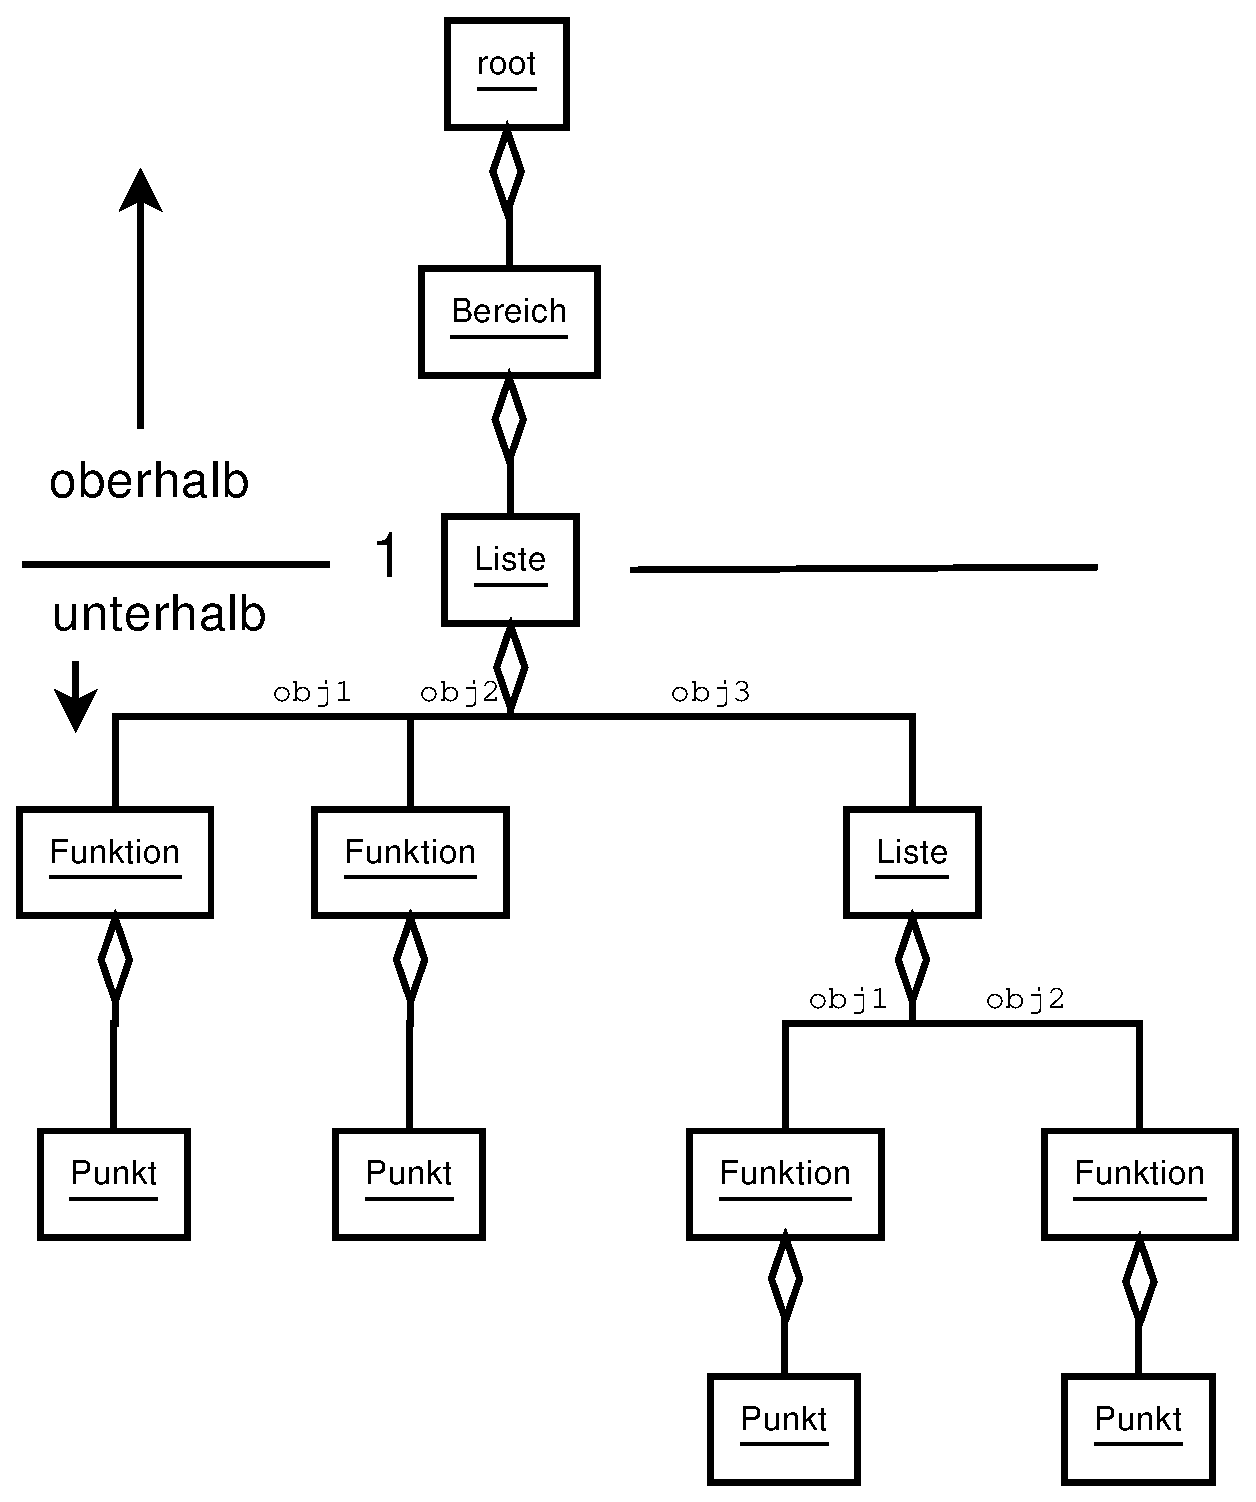
\includegraphics[scale=0.5]{oberhalb_unterhalb}
\end{center}
\caption{Beispiel f"ur oberhalb und unterhalb in einem Fib-Objekt}
\label{figDirectionFibElements}
\end{figure}


\subsection{Ordnung der Fib-Elemente}\index{Ordnung!Fib-Elemente}
\label{secOrderFibElements}

Auf den Definitionen von ``unterhalb'' und ``oberhalb'' in einem Fib-Objekt wird die Ordnung der Fib-Elemente aufgebaut. Jedem Fib-Element im vollst"andige Fib-Objekt wird eine eindeutige nat"urliche Zahl zugeordnet. Wenn in einem Fib-Objekt $N$ Elemente existieren, werden den Fib-Elementen im Fib-Objekt die Zahlen $1$ bis $N$ zugeordnet. Fib-Elementen unterhalb eines Fib-Elements werden h"ohere Werte zugeordnet.

Bei Listenelementen haben Unterobjekte $Obj_U$ des Listenelements mit einer h"oheren Nummer $U$ als ein anderes Unterobjekt $Obj_K$ ($U>K$) auch h"ohere Nummern f"ur ihre enthaltenden Elemente, als die Elemente in $Obj_K$. Die root-Elemente werden in der Ordnung genauso behandelt wie Listenelemente, wobei das Haupt-Fib-Objekt das erste Unterobjekt ist, dem die Unter-root-Objekte in ihrer Reihenfolge (im root-Element) folgen.

Das selbe gilt f"ur alle anderen Zweigelemente. Die oben vorgestellte Syntax gibt dabei die Reihenfolge der Unterobjekte vor.

In Abbildung \ref{figOrderFibElements} ist eine Beispielobjekt mit den zugeh"origen Zahlen (links neben den Elementen) der Ordnung der Fib-Element dargestellt.

\begin{figure}[htbp]
\begin{center}
  \includegraphics[scale=0.5]{order_elements}
\end{center}
\caption{Beispiel f"ur die Ordnung der Fib-Elemente}
\label{figOrderFibElements}
\end{figure}


\subsection{Ordnung bestimmter Fib-Elemente}\index{Ordnung!bestimmte Fib-Elemente}

Auch Fib-Elemente eines bestimmten Typs sind nat"urliche Zahlen einer Ordnung zugeordnet. Diese Ordnungen orientieren sich an der Ordnung der Fib-Elemente. Wenn in einem korrekten Fib-Objekt $N$ Fib-Elemente eines Typs existieren, so sind den Fib-Elementen dieses Typs die Zahlen $1$ bis $N$ zugeordnet. Ist ein Fib-Element $Elm_1$ in der Ordnung der Fib-Elemente ein h"oherer Wert zugeordnet (als einem anderen Fib-Element $Elm_2$ des gleichen Typs), so ist ihm ($Elm_1$) auch in der Ordnung der Fib-Elemente des gleichen Typs ein h"oherer Wert zugeordnet (als dem anderen Fib-Element $Elm_2$).

In Abbildung \ref{figOrderSpecialFibElements} ist eine Beispielobjekt mit den zugeh"origen Zahlen (links neben den Elementen) der Ordnungen der einzelnen Fib-Element dargestellt.

\begin{figure}[htbp]
\begin{center}
  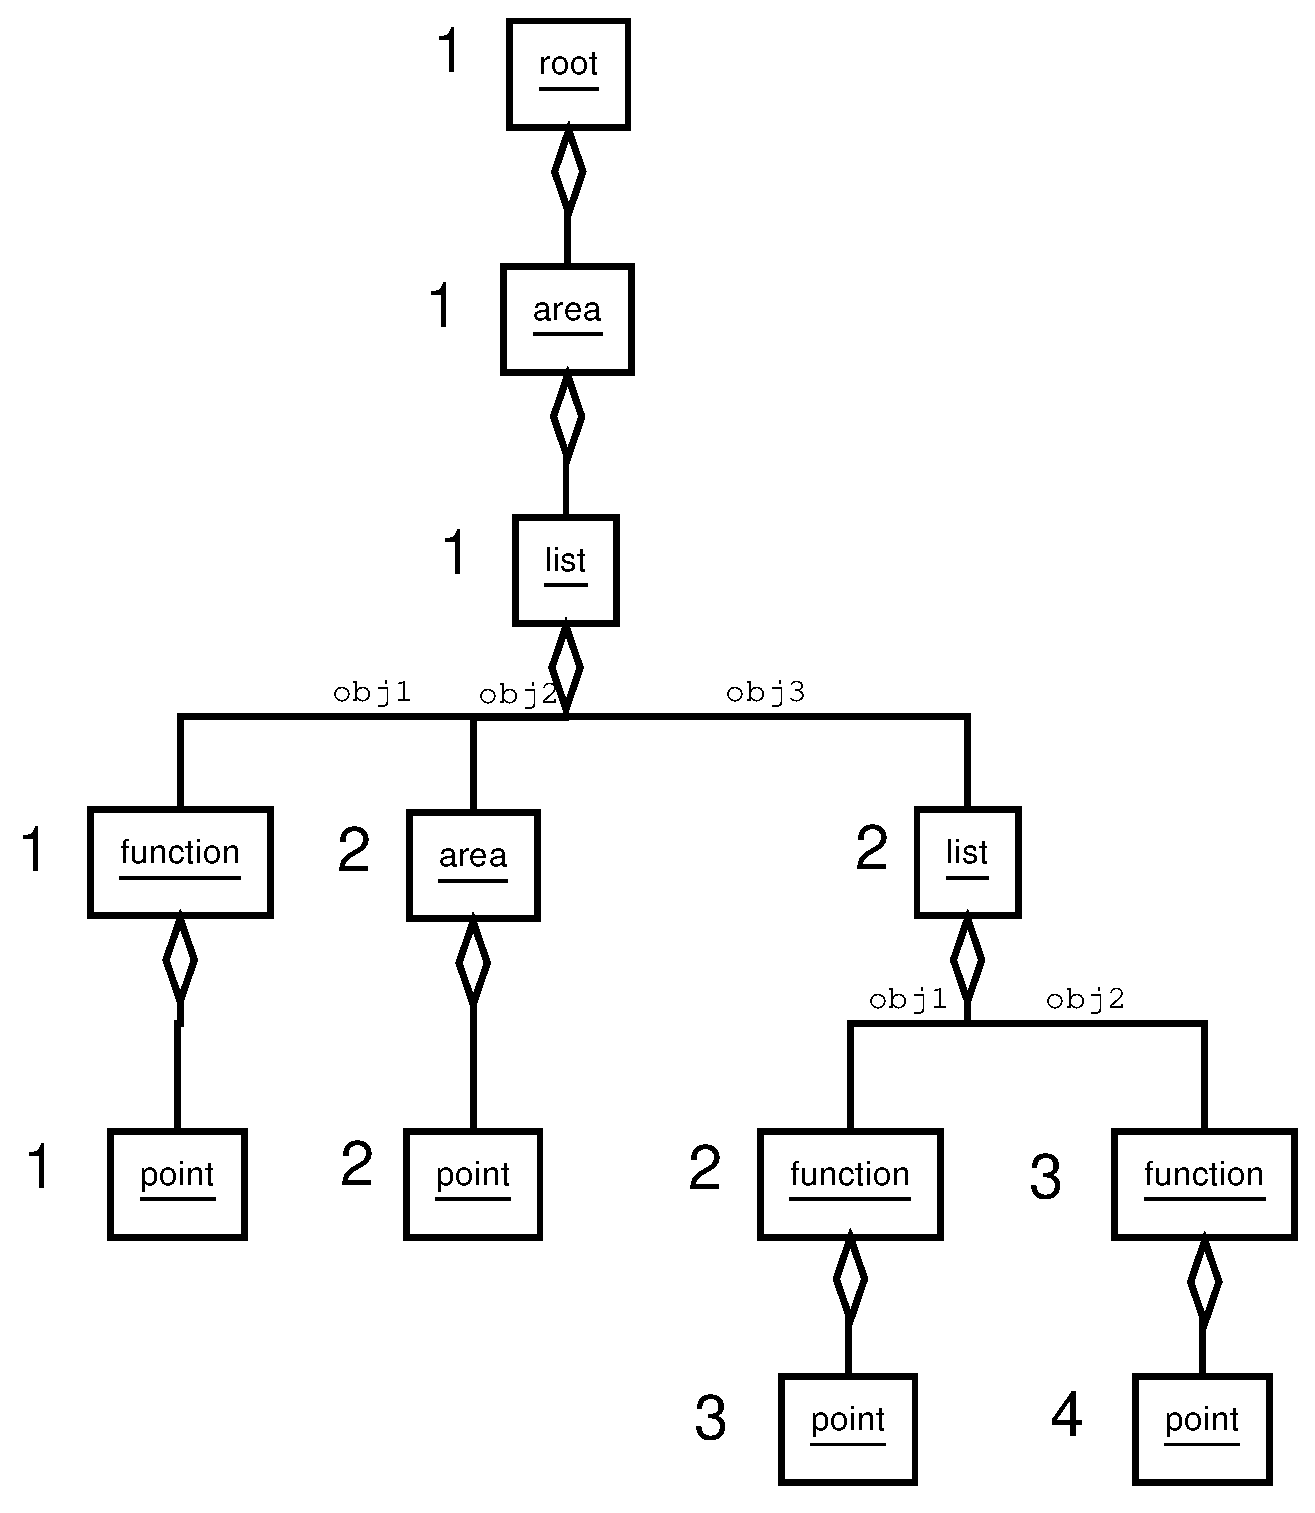
\includegraphics[scale=0.5]{order_special_elements}
\end{center}
\caption{Beispiel f"ur die Ordnung bestimmter Fib-Elemente}
\label{figOrderSpecialFibElements}
\end{figure}


\subsection{Ordnung der Verschiebungspunkte}\index{Verschiebungspunkte}\index{Ordnung!Verschiebungspunkte}

Eine weitere Ordnung betrifft alle Fib-Elemente, die verschoben werden k"onnen. Diese werden Verschiebungspunkte genannt.
Die Ordnungen der Verschiebepunkte orientieren sich an der Ordnung der Fib-Elemente. Wenn in einem vollst"andigen Fib-Objekt $N$ Verschiebepunkte existieren, so sind den Verschiebepunkte, die Zahlen $1$ bis $N$ zugeordnet. Ist ein Fib-Element in der Ordnung der Fib-Elemente ein h"oherer Wert zugeordnet, so ist ihm auch in der Ordnung der Verschiebepunkte ein h"oherer Wert zugeordnet.

\bigskip\noindent
Fib-Elemente, welche verschoben werden k"onnen und Verschiebepunkte darstellen, sind alle Zweigelemente (limb Elemente; sie enthalten genau ein Unterobjekt):
\begin{itemize}
 \item Eigenschaftselement (siehe Abschnitt \ref{fibProperty} auf Seite \pageref{fibProperty})
 \item Anmerkungselemente (siehe Abschnitt \ref{fibComment} auf Seite \pageref{fibComment})
 \item Bereichselemente (siehe Abschnitt \ref{fibArea} auf Seite \pageref{fibArea})
 \item Funktionselemente (siehe Abschnitt \ref{fibFunction} auf Seite \pageref{fibFunction})
 \item Fib-Element, um Definitionsbereichseigenschaften abzurufen (siehe Abschnitt \ref{fibDomeinProperties} auf Seite \pageref{fibDomeinProperties})
 \item Set-Element (siehe Abschnitt \ref{secFibSetElement} auf Seite \pageref{secFibSetElement})
 \item Matrixelement (siehe Abschnitt \ref{secFibMatrixElement} auf Seite \pageref{secFibMatrixElement})
\end{itemize}

\bigskip\noindent
Fib-Elemente, welche nicht verschoben werden k"onnen und damit keine Verschiebepunkte darstellen, sind:
\begin{itemize}
 \item Alle Blattelemente:
 \begin{itemize}
  \item Punkte (siehe Abschnitt \ref{fibPoint} auf Seite \pageref{fibPoint})
  \item Fib-Elemente f"ur externe Unterobjekte (siehe Abschnitt \ref{fibSubobject} auf Seite \pageref{fibSubobject})
 \end{itemize}
 \item Alle Verzweigungselemente:
 \begin{itemize}
  \item Root-Element (siehe Abschnitt \ref{fibRootElement} auf Seite \pageref{fibRootElement})
  \item Listenelement (siehe Abschnitt \ref{fibList} auf Seite \pageref{fibList})
  \item Das Fib-Element, um externe Objekte aufzurufen (siehe Abschnitt \ref{fibExtObject} auf Seite \pageref{fibExtObject})
  \item Bedingungen mit dem if-Element (siehe Abschnitt \ref{secFibIf} auf Seite \pageref{secFibIf})
 \end{itemize}
\end{itemize}

In Abbildung \ref{figOrderMovePoints} ist ein Beispielobjekt mit den zugeh"origen Zahlen (links neben den Elementen) der Ordnung der Verschiebepunkte dargestellt.

\begin{figure}[htbp]
\begin{center}
  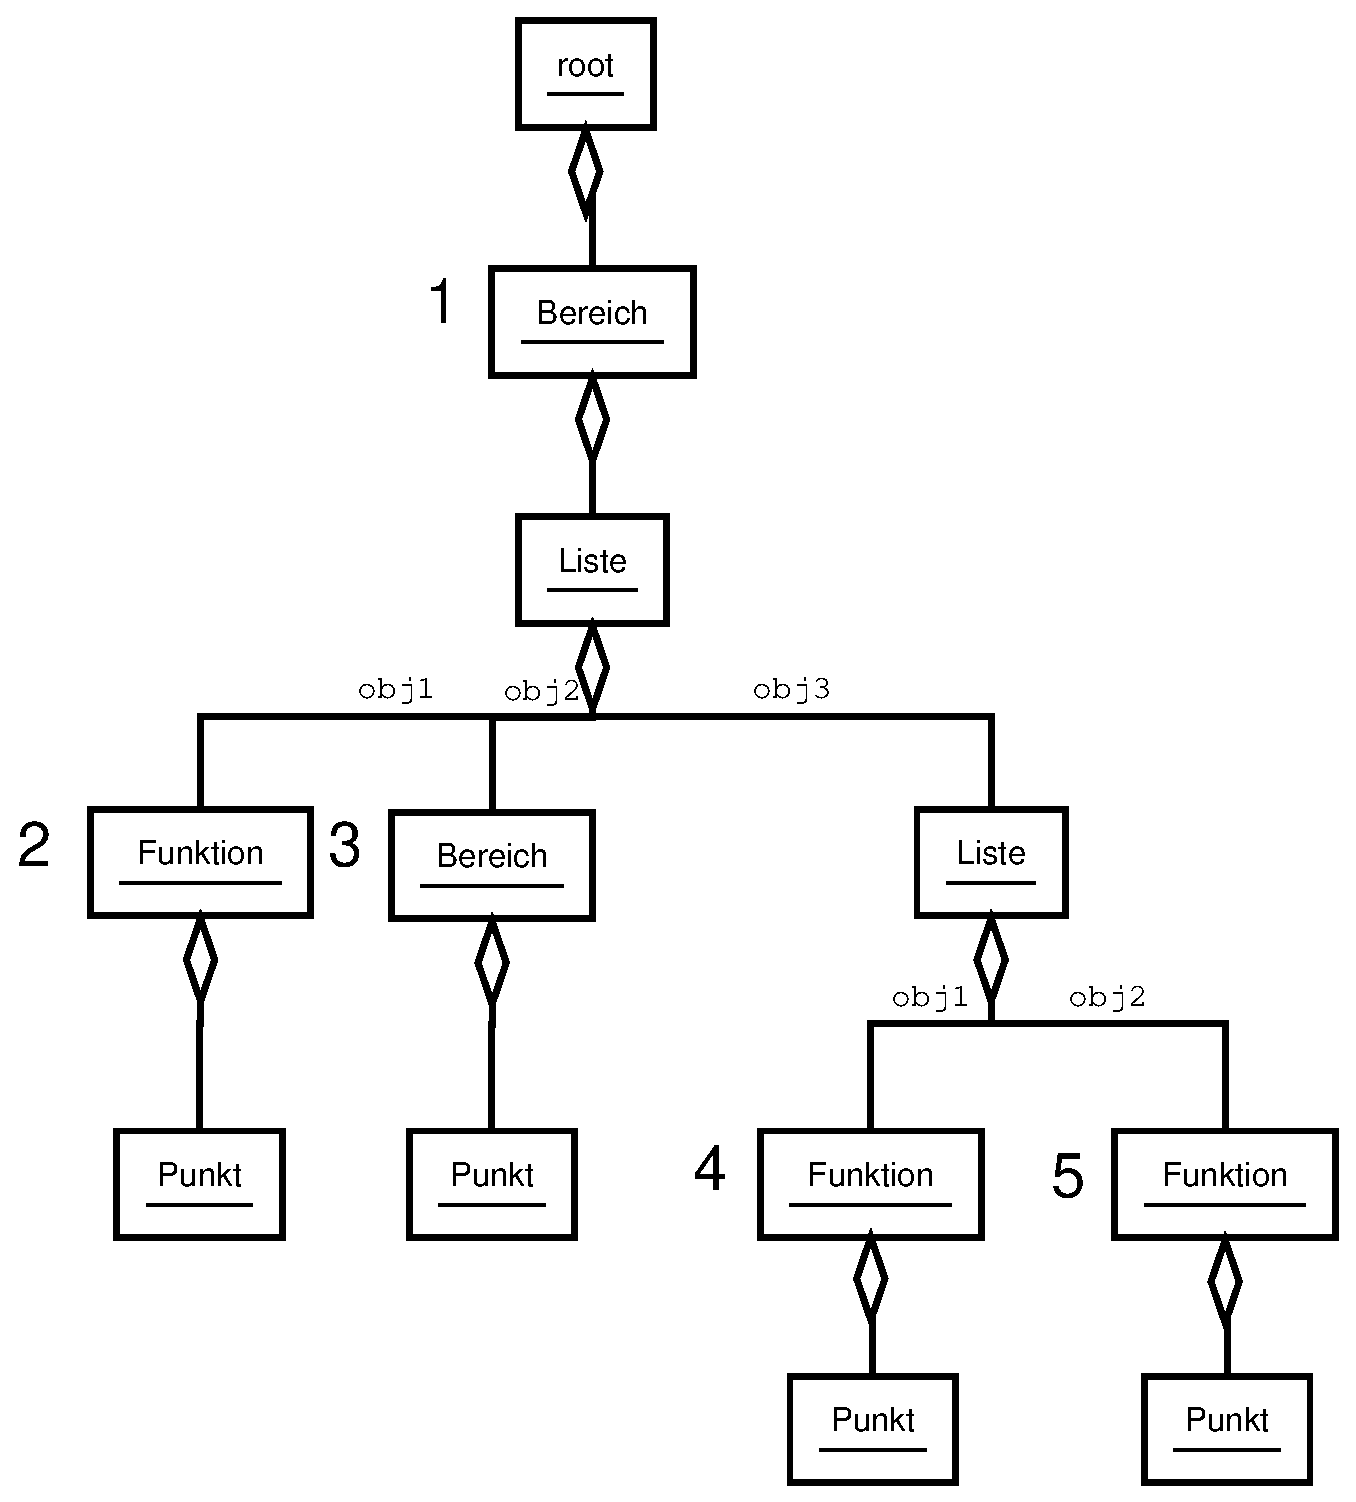
\includegraphics[scale=0.5]{order_move_points}
\end{center}
\caption{Beispiel f"ur die Ordnung der Verschiebungspunkte}
\label{figOrderMovePoints}
\end{figure}


\subsection{Definition Teilobjekt}\index{Teilobjekt|(}

Jedes Objekt, das ein ganzer Zweig (z. B. Unterlistenobjekt, Haupt-Fib-Objekt oder Unter-root-Objekt) eines Verzweigungselements ist, ist Teil eines Teilobjekts. Weiterhin geh"oren zum Teilobjekt alle root-Elemente, in denen es enthalten ist oder die es "uber externe Objekte benutzt. Auch Fib-Elemente, die Variablen definieren, welche in dem Teilobjekt verwendet werden, geh"oren dazu.
Die Vereinigung zweier Teilobjekte ist wieder ein Teilobjekt.
Das ganze Fib-Objekt selbst ist auch ein Teilobjekt.
Ein Teilobjekt kann immer zu einem Multimediaobjekt ausgewertet werden.

Ein \textbf{echtes Teilobjekt}\index{Teilobjekt!echtes} ist ein Teilobjekt, das nicht das (ganze) Fib-Objekt selbst ist.

Ein \textbf{einfaches Teilobjekt}\index{Teilobjekt!einfach} ist ein echtes Teilobjekt, das nur ein Blatt mit einem Punktobjekt enth"alt.

Ein \textbf{zusammenh"angendes Teilobjekt}\index{Teilobjekt!zusammenh"angendes} ist ein echtes Teilobjekt, welches das gesamte Objekt eines Arms, genau eines Verzweigungselements (z. B. Listenelements oder root-Elements) enth"alt und die ben"otigten Elemente "uber diesem. Insbesondere ist jedes einfache Teilobjekt ein zusammenh"angendes Teilobjekt.

Um ein zusammenh"angendes Teilobjekt zu erzeugen, kann aus dem ganzen Fib-Objekt ein Verzweigungselement (z. B. Listenelement oder root-Element) gel"oscht und durch ein in ihm enthaltendes Unterobjekt ersetzt werden. Das erzeugte Teilobjekt muss nat"urlich korrekt sein, um ein zusammenh"angendes Teilobjekt zu sein. (Es darf beispielsweise bei einem root-Element nicht das Haupt-Fib-Objekt gel"oscht werden, und wenn ein root-Element gel"oscht wird, und das n"achste Haupt-Fib-Objekt oberhalb durch sein Haupt-Fib-Objekt ersetzt wird, m"ussen die Definitionsbereiche des ersetzten root-Elements vom n"achsten enthaltenden root-Element "ubernommen werden.)

Mit Abbildung \ref{figOrderFibElementsPartobjects} sei diese Definition an einem Beispiel eines Fib-Objekts dargestellt. Im Nachfolgenden werden einige Beispiele f"ur unterschiedliche Typen von Teil\-objekte in Abbildung \ref{figOrderFibElementsPartobjects} gegeben, wobei f"ur die Fib-Elemente ihre Nummern (aus der Fib-Elementordnung bzw. der Abbildung \ref{figOrderFibElementsPartobjects}) angegeben werden. Weiterhin wird festgelegt, dass das Punktelement mit der Nummer $10$ nicht die Variable benutzt, welche das Bereichselement mit der Nummer $2$ definiert. Alle anderen Variablen werden in den Punkten ben"otigt, welche unter der jeweiligen Variablendefinition stehen.

\begin{figure}[htbp]
\begin{center}
  \includegraphics[scale=0.5]{order_elements}
\end{center}
\caption{Beispiel Objekt f"ur Teilobjekte}
\label{figOrderFibElementsPartobjects}
\end{figure}


\bigskip\noindent
Teilobjekte:
\begin{itemize}
 \item 1; 2; 4; 5
 \item 1; 2; 6; 7
 \item 1; 2; 3 (nur Unterobjekt $1$ und $2$); 4; 5; 6; 7
 \item 1; 9; 10
 \item 1; 2; 8; 9; 10; 11; 12
 \item 1; 2; 3 (nur Unterobjekt $1$ und $3$); 4; 5; 8; 9; 10; 11; 12
 \item 1; 2; 3 (nur Unterobjekt $1$ und $3$); 4; 5; 11; 12
 \item (alle Fib-Elemente) 1; 2; 3; 4; 5; 6; 7; 8; 9; 10; 11; 12
\end{itemize}

Echte Teilobjekte:
\begin{itemize}
 \item 1; 2; 4; 5
 \item 1; 2; 6; 7
 \item 1; 2; 3 (nur Unterobjekt $1$ und $2$); 4; 5; 6; 7
 \item 1; 9; 10
 \item 1; 2; 8; 9; 10; 11; 12
 \item 1; 2; 3 (nur Unterobjekt $1$ und $3$); 4; 5; 8; 9; 10; 11; 12
 \item 1; 2; 3 (nur Unterobjekt $1$ und $3$); 4; 5; 11; 12
\end{itemize}

Einfache Teilobjekte:
\begin{itemize}
 \item 1; 2; 4; 5
 \item 1; 2; 6; 7
 \item 1; 9; 10
 \item 1; 2; 11; 12
\end{itemize}

Zusammenh"angende Teilobjekte:
\begin{itemize}
 \item 1; 2; 4; 5
 \item 1; 2; 6; 7
 \item 1; 9; 10
 \item 1; 2; 11; 12
 \item 1; 2; 8; 9; 10; 11; 12
\end{itemize}


\subsection{Die Ordnung der zusammenh"angenden Teilobjekte}
\label{secOrderPartobjects}

Auch auf den zusammenh"angenden Teilobjekten gibt es eine Ordnung. Diese wird im Nachfolgenden auch Ordnung der Teilobjekte gennant, da es f"ur die anderen Arten von Teilobjekten keine eigene Ordnung gibt.

Die Ordnungen der (zusammenh"angenden) Teilobjekte orientieren sich an der Ordnung der Fib-Elemente. Wenn in einem vollst"andigen Fib-Objekt $N$ zusammenh"angende Teilobjekte existieren, so sind den zusammenh"angenden Teilobjekten die Zahlen $1$ bis $N$ zugeordnet.
Je gr"o"ser die Nummer eines zusammenh"angenden Teilobjekts ist, desto gr"o"ser ist auch die kleinste Nummer in Ordnung der Fib-Elemente, der Fib-Elemente in ihm.
%Ist einem Fib-Element in der Ordnung der Fib-Elemente ein h"oherer Wert zugeordnet, so ist dem Teilobjekt, welches unter den Teilobjekten, die das Fib-Element enth"alt, die gr"o"ste Nummer in der Ordnung der Teilobjekte hat, auch in der Ordnung der zusammenh"angenden Teilobjekt ein h"oherer Wert zugeordnet.
Oder auch: Ist dem obersten Fib-Element des Unterobjekts, "uber das ein zusammenh"angendes Teilobjekt definiert ist, ein h"oherer Wert zugeordnet, so ist auch dem definierten Teilobjekt ein h"oherer Wert zugeordnet.

In Abbildung \ref{figOrderPartobjekts} ist ein Beispielobjekt mit den zugeh"origen Zahlen (links neben den definierenden Unterobjekten der Teilobjekte) in der Ordnung der Teilobjekte dargestellt.

\begin{figure}[htbp]
\begin{center}
  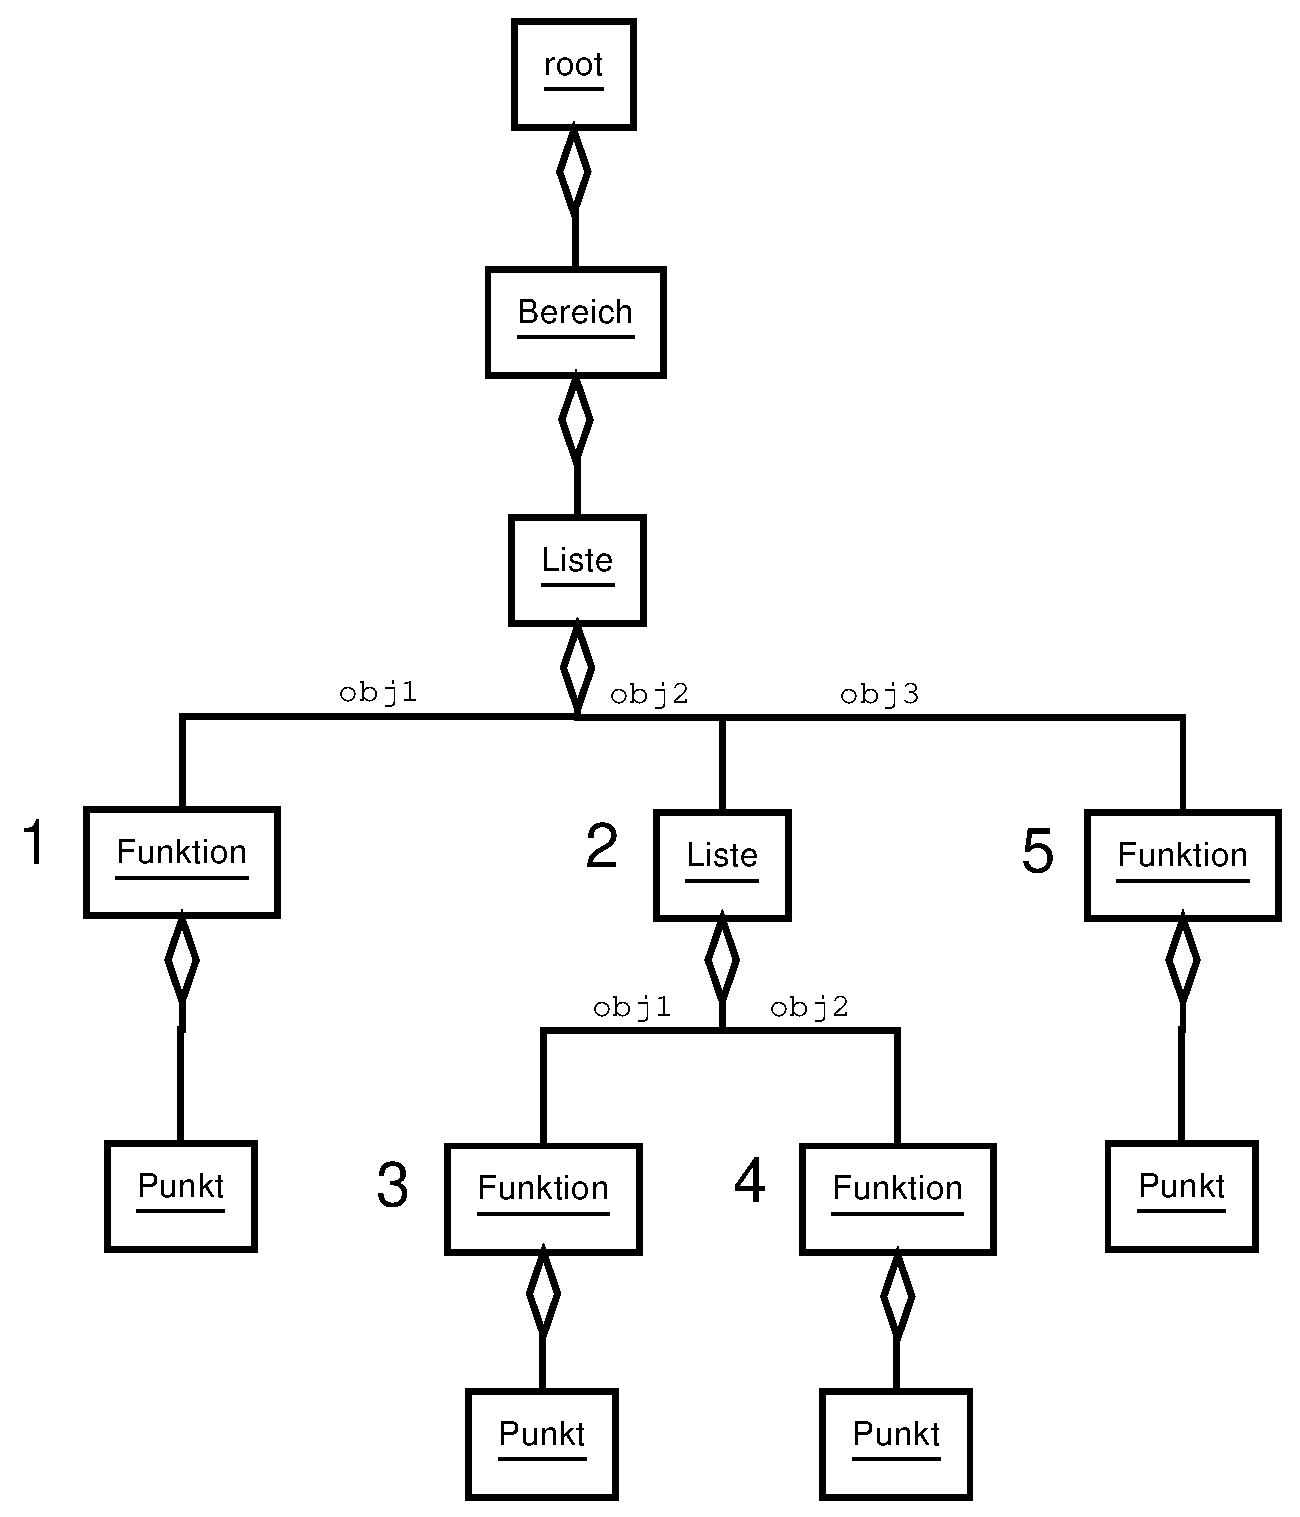
\includegraphics[scale=0.5]{order_partobjects}
\end{center}
\caption{Beispiel f"ur die Ordnung der zusammenh"angenden Teilobjekte}
\label{figOrderPartobjekts}
\end{figure}


\index{Teilobjekt|)}

\subsection{Definition Fib-Multimediaobjekt}\index{Fib-Multimediaobjekt}

Wird der Ausdruck Fib-Multimediaobjekt benutzt, ist damit ein Fib-Objekt mit Schwerpunkt auf dem Multimediaobjekt, das es repr"asentiert, gemeint.


\subsection{Definition richtiges Fib-Multimediaobjekt}\index{Fib-Multimediaobjekt!richtiges}

Ein richtiges Fib-Multimediaobjekt ist ein Fib-Objekt, welches das originale Multimediaobjekt, das es repr"asentieren soll, vollst"andig wiedergibt. Wenn also das Multimediaobjekt, welches das Fib-Objekt repr"asentiert, und das originale Multimediaobjekt verglichen werden, kann kein Unterschied zwischen ihnen feststellt werden.



%TODO: in welche Sprache kontextfrei oder regul"ar?



%TODO
%%
% Copyright (c) 2008 Betti "Osterholz
%
% Permission is granted to copy, distribute and/or modify this document
% under the terms of the GNU Free Documentation License, Version 1.2 or
% any later version published by the Free Software Foundation;
% with no Invariant Sections, no Front-Cover Texts, and no Back-Cover Texts.
%
% A copy of the license is included in the file ``fdl.tex'' .
%

\section{Theoretische Aussagen zur Fib-Multi\-media\-be\-schrei\-bungs\-sprache}
\label{secTheoreticFib}

Es folgen einige theoretische Aussagen zur Fib-Multimediabeschreibungssprache, f"ur die aber aus Zeitgr"unden meistens nicht ein vollst"andiger Beweis angef"uhrt wird. Mit diesen Aussagen soll ein besseres Verst"andnis der Fib-Multimediasprache erreicht werden.


\subsection{M"achtigkeit der Fib-Multimediasprache auf Bilder}
\label{secPowerOfFibOnPictures}

Mit der Fib-Multimediasprache k"onnen alle als Rastergrafik darstellbaren Bilder dargestellt werden. Bilder, die als Rastergrafik darstellbar sind, sind die am h"aufigsten verwendeten Bilder in der elektronischen Datenverarbeitung. Dazu geh"oren unter anderem Windows Bitmap (BMP, Dateiendung: .bmp), JPEG File Interchange Format (JFIF, Dateiendung: .jpg) und Portable Network Graphics (PNG, Dateiendung: .png).

Allein mit dem Punktelement und dem Listenelement lassen sich bereits alle m"oglichen Rastergrafiken darstellen.

\bigskip\noindent
\textbf{Beweis:}
Eine Rastergrafik (euklidisch, zweidimensional, diskret) kann als Matrix dargestellt werden, in der die Spalte die x-Koordinate, die Zeile die y-Koordinate des Punktes angibt und die Werte die Farben der Punkte angeben. Die Anzahl der Punkte in der Rastergrafik ist endlich. Um diese Punkte durch Fib-Multimediasprache darzustellen, ist ein root-Element zu erzeugen, das die Eigenschaften der Rastergrafik enth"alt (Gr"o"se bzw. Dimensionsdefinitionsbereich usw.). In diesem root-Element ist als Haupt-Fib-Objekt ein Listenelement einzuf"ugen, welches f"ur jeden Punkt des Bildes ein Unterobjekt enth"alt. Dieses Unterobjekt besteht nur aus einem Eigenschaftselement, das die Farbe des Punktes kodiert, und einem enthaltenden Punktelement, welches die Position des Punktes kodiert. So gibt es f"ur jeden Punkt in der Rastergrafik einen entsprechenden Punkt im erzeugten Fib-Objekt, womit das Fib-Objekt die Rastergrafik repr"asentiert.

Eine Abbildung in die Fib-Multimediasprache kann beispielsweise mit dem im Listing \ref{alleBild} dargestellten Algorithmus geschehen (Pseudo-C).

\begin{flushleft}
Dabei beginnt die Indizierung der Matrix mit (0,0).

Der Farbwert der Koordinate (x,y) kann mit \verb|matrix[ x, y]| bestimmt werden. Mit der Funktion \verb|getColorVector()| wird aus dem Matrix-Farbwert ein Fib-Farbvektor generiert.

Die Syntax der Fib-Objekte entspricht der im Abschnitt \ref{partFibLanguage} auf Seite \pageref{partFibLanguage} angesprochenen m"oglichen Syntax.
\end{flushleft}

\begin{lstlisting}[language=C, numbers=left, frame=single, caption={Algorithmus zur Erzeugung eines korrekten Fib-Objekts aus einer Bildmatrix}, label={alleBild}, breaklines, basicstyle=\footnotesize\ttfamily, numberstyle=\tiny]
void translate( matrix ){

   int xmax = Anzahl der Spalten der Matrix;
   int ymax = Anzahl der Zeilen der Matrix;
   Fib_Objekt_Pointer obj=new root();

   //Eigenschaften der Rastergrafik setzen
   obj->setBild( xmax, ymax, Farbschema);

   list hauptliste=new list()

   obj->insertMainObject( hauptliste )

   for( int x = 0; x == xmax; x = x + 1 ){

      for( int y = 0; y == xmax; y = y + 1 ){
         hauptliste->insertObject( property( getColorVector( matrix[x,y] ) , p( (x,y) ) ) );
      };
   };
};
\end{lstlisting}

\bigskip\noindent
Da die Erweiterung mit Funktionen und anderen Elementen optional ist, wird mit dem angegebenen Algorithmus ein korrektes Fib-Objekt erzeugt.

\bigskip\noindent
Zu jedem Punkt in der Matrix gibt es einen gleichfarbigen Punkt im Fib-Objekt mit der entsprechenden Koordinate, aber es gibt keinen Punkt im Fib-Objekt, der nicht in der Matrix vorhanden ist, denn jede Koordinate der Matrix wird mit den zwei for-Schleifen durchlaufen. Dadurch wird f"ur jede Koordinate und damit auch f"ur jeden Punkt in der Rastergrafik ein Punkt im Fib-Objekt eingef"ugt. Somit gibt es f"ur jeden Punkt in der Rastergrafik einen entsprechenden Punkt in dem Fib-Objekt.
Da nur Koordinaten der Matrix in den for-Schleifen durchlaufen werden und nur f"ur diese die entsprechenden Punkte in das Fib-Objekt eingef"ugt werden, existieren nur Punkte die auch in der Matrix auftauchen und damit auch nur Punkte im Fib-Objekt die auch in der Rastergrafik vorkommen.
Es gibt also nur die Punkte aus der Originalrastergrafik im Fib-Objekt und nur diese.
Damit repr"asentieren das Fib-Objekt und die Originalrastergrafik die gleiche Rastergrafik. Deshalb k"onnen alle Rastergrafiken auch mit der Fib-Multimediasprache dargestellt werden.

Ein mit dem Algorithmus generiertes Fib-Objekt, das einer Originalrastergrafik entspricht, stellt eine obere Grenze der minimalen Gr"o"se m"oglicher entsprechender Fib-Objekte da. Das hei"st, jede Rastergrafik kann durch ein Fib-Objekt repr"asentiert werden, das genauso gro"s ist, wie ein Fib-Objekt f"ur die Rastergrafik, das mit dem oben aufgef"uhrten Algorithmus generiert wurde, n"amlich das generierte Fib-Objekt. Es gibt aber wahrscheinlich noch k"urzere Fib-Objekte f"ur die Rastergrafik.

\begin{flushleft}
Damit ist die minimale Gr"o"se eines Fib-Objekts f"ur eine Rastergrafik maximal:

$Fib\_max_{min}$ = (Anzahl der Pixel im Bild) $* [$(Gr"o"se eines Punktelements) + (Gr"o"se eines Eigenschaftselements f"ur das entsprechende Farbschema)$]$ + (Gr"o"se eines Listenelements)+ (Gr"o"se eines root-Elements mit gesetzten Werten)

\bigskip\noindent
Beispiel: Dargestellt werden soll ein Bild 8 x 8 = 256 Pixel mit 3 Byte f"ur die Farbe (RGB), 1 Byte f"ur die Position (f"ur jede Richtung x und y 4 Bit = 8 m"ogliche Werte) und 1 Byte f"ur den Objektnamen (z. B. ``l'' f"ur Listelemente und ``p'' f"ur Punktelemente). Klammern werden nicht ben"otigt, da alle Teile eine feste L"ange haben. (Die Annahmen "uber die Gr"o"sen der Fib-Objekt-Elemente wird hier abgesch"atzt. Bei einer Implementierung sind sicherlich bessere (/kleinere) Werte m"oglich.)
\begin{itemize}
 \item F"ur einen Punktelement werden 2 Byte ben"otigt (1 Byte Position + 1 Byte Elementname).
 \item F"ur eine Eigenschaftselement werden 4 Byte ben"otigt (3 Byte Farbe + 1 Byte Elementname).
 \item F"ur ein Listenelement werden 9 Byte ben"otigt ( 8 Byte f"ur Angabe der Anzahl der Unterobjekte + 1 Byte Elementname).
 \item F"ur das root-Element werden 256 Bytes ben"otigt. (Da viele Teile des root-Elements leer sind und nur der Definitionsbereichen f"ur 2 Dimensionen und die RGB-Farbdefinitionsbereiche angegeben werden m"ussen, sollten 256 Bytes gen"ugen.)
\end{itemize}

\bigskip\noindent
Rechnung:
$256 (Pixel) * (2 Bytes + 4 Bytes) + 9 Bytes + 256 Bytes = 1801 Bytes$

\bigskip\noindent
Das Bild kann also auf jeden Fall mit einem 1801 Byte gro"sen Fib-Objekt dargestellt werden. Es sind davon abweichende k"urzere Fib-Objekt-Darstellungen m"oglich. Die 1801 Byte sind also die Obergrenze f"ur die minimale Gr"o"se, mit der das Bild mit einem Fib-Objekt dargestellt werden kann.

\bigskip\noindent
Zum Vergleich: Der Speicherbedarf einer Rastergrafik als Bitmap (nur Punkt-Informationen) betr"agt mindestens
(Anzahl der Pixel im Bild) * (Gr"o"se eines Farbwertes)

\bigskip\noindent
F"ur das obige Beispiel ergibt sich: $256 (Pixel) * 3 Bytes = 768 Bytes$

\bigskip\noindent
Das ist ungef"ahr die H"alfte der 1801 Byte der Obergrenze f"ur die minimale Fib-Objekt-Darstellung.

\bigskip\noindent
Indem die Matrix auf 3 Dimensionen erweitert wird, kann die Aussage "uber die Darstellbarkeit aller Rastergrafiken leicht auf Sequenzen von Rastergrafiken (z. B. die Bilder von Filmen) erweitert werden.

\end{flushleft}


\subsection{M"achtigkeit von Fib}

\textbf{Satz: Die Menge der m"oglichen Fib-Objekte ist abz"ahlbar unendlich.}

\bigskip\noindent
Beweis Skizze f"ur die Abz"ahlbarkeit:

\noindent
Jedes Fib-Objekt kann mit einer endlichen Anzahl von Buchstaben und damit auch Bits oder Zahlen repr"asentiert werden, und die Menge dieser ist abz"ahlbar.
Das folgt daraus, dass die Anzahl der Fib-Elemente in einem Fib-Objekt immer abz"ahlbar ist und jedes Fib-Element aus abz"ahlbar vielen Teilen besteht, welche selbst abz"ahlbar sind, es gibt z. B. nur ganze oder rationale Zahlen, und auch die Menge der Variablen ist abz"ahlbar.

\bigskip\noindent
Beweis Skizze f"ur ``unendlich'':

\noindent
Es k"onnen alle nat"urlichen Zahlen durch Fib-Objekte repr"asentiert werden. Im Nachfolgendem ist eine m"ogliche Darstellungsart von beliebigen nat"urlichen Zahlen mithilfe von Fib-Objekten beschrieben.

Ein Punktobjekt alleine stellt die nat"urliche Zahl 0 da.
Wird ein Fib-Objekt in ein neues Funktionselement eingesetzt, stellt das entstehende Fib-Objekt den Nachfolger des urspr"unglichen Fib-Objekts da.
Damit werden die 0 und die Nachfolgefunktion in der Fib-Multimediasprache nachgebildet, und es k"onnen damit alle nat"urlichen Zahlen dargestellt werden. Da die Menge der nat"urlichen Zahlen unendlich ist, muss die Menge der Fib-Objekte auch unendlich sein.

\bigskip\noindent
Jedes Multimediaobjekt wird sogar durch eine abz"ahlbar unendliche Menge von Fib-Objekten repr"asentiert, denn es kann an ein Fib-Objekt, das ein Multimediaobjekt repr"asentiert, jedes beliebige Fib-Objekt mit einem Listenelement angeh"angt werden, solange dieses die Multimediaobjektdarstellung nicht ver"andert. Es k"onnte z. B. beliebig oft an ein Fib-Objekt eine Kopie von sich selbst mit Hilfe eines Listenelements angef"ugt werden, ohne das Multimediaobjekt zu ver"andern.


\subsection{Jedes vollst"andige Fib-Objekt kann als ein Multimediaobjekt dargestellt werden}
\label{alleBilder}

Es wird in diesem Abschnitt aufgezeigt, dass es m"oglich ist, jedes vollst"andige Fib-Objekt (siehe Abschnitt \ref{secFullFibObject} auf Seite \pageref{secFullFibObject}) immer so zu interpretieren (in ein Multimediaobjekt zu "ubersetzen), dass nur g"ultige Multimediaobjekte eines bestimmten Typs (z. B. RGB-Bilder mit 100 x 100 Pixel) entstehen k"onnen. Dabei wird die schon angesprochene Einschr"ankung bez"uglich der Multimediadaten vorrausgesetzt, dass die Multimediadaten als Eigenschaften von Punkten eines endlichen, euklidischen, diskreten (es gibt kleinste Einheiten) Raumes darstellbar sind. Diese Einschr"ankung ist nicht sehr gro"s, da sie (fast) keine der heutzutage "ublichen Multimediadaten ausgrenzt. Die Multimediadaten k"onnen also Bilder, Ton und Filme darstellen.

Mit der Einschr"ankung, dass der Abstand/Unterschied zwischen zwei Eigenschaften des gleichen Typs immer als Zahlenwert bestimmt werden kann, k"onnen zwei Multimediaobjekte mit den gleichen Dimensionen immer verglichen werden. Zwei Multimediaobjekte haben die gleichen Dimensionen, wenn f"ur jeden Punkt in dem einem Multimediaobjekt genau ein entsprechender Punkt im jeweils anderen Multimediaobjekt existiert.

Die Voraussetzung des vollst"andigen Fib-Objekts ist n"otig, um zu gew"ahrleisten, dass das Fib-Objekt immer auswertbar ist. Da die Vollst"andigkeit eines Fib-Objekts "uber die in Teil \ref{partFibLanguage} dargestellte Syntax gepr"uft werden kann, ist die Vollst"andigkeit eines Fib-Objekts immer feststellbar. Nicht vollst"andige Fib-Objekte sollten von Algorithmen bzw. den genetischen Operatoren nicht erzeugt werden.

Wenn nun bei einem Fib-Objekt die Dimensionen an die eines Multimediaobjekts angepasst werden (dies sollte immer m"oglich sein), ist das Fib-Objekt immer mit dem Multimediaobjekt vergleichbar, da es selbst immer als Multimediaobjekt dargestellt werden kann und zwei Multimediaobjekte mit den gleichen Dimensionen immer verglichen und die "Ahnlichkeit zueinander bewertet werden kann.

Anmerkung: Dies ist f"ur genetische Algorithmen vorteilhaft. Bei einigen anderen Darstellungsformen, die durch genetische Algorithmen erzeugt werden, k"onnen ung"ultige Objekte (z. B. Programme) entstehen, bei denen eine genauere(/r) Bewertung/Vergleich nicht m"oglich ist. Eine Population in dieser Darstellungsform kann dann, z. B. eine gro"se Klasse von ung"ultigen Objekten haben, die alle gleich schlecht sind und damit bei der Selektion gleich ber"ucksichtigt werden. Wenn dann die Population nur aus ung"ultigen Individuen besteht, ist die Auswahl eines besseren Individuums unm"oglich. Der genetische Algorithmus befindet sich dann sozusagen auf einer (Fitness-)Ebene, von der er nur noch schwer herunterfinden kann.

\bigskip\noindent
Beweis, dass jedes korrekte Fib-Objekt als ein Multimediaobjekt (eines bestimmten Typs, z. B. als Bild) dargestellt werden kann: 
Ausgangspunkt ist, dass ein Multimediaobjekt (euklidisch, zweidimensional, diskret) als endliche Menge von Punkten mit ihren (endlich vielen) Eigenschaften dargestellt werden kann. Da es nur endlich viele Punkte mit nur endlich vielen Eigenschaften gibt, ist eine solche endliche Menge immer konstruierbar.

Eine solche endliche Menge von Punkten mit ihren (endlich vielen) Eigenschaften erzeugt auch jedes korrekte Fib-Objekt. Punkte die in dieser Menge zu viel sind, um ein Multimediaobjekt zu repr"asentieren, werden aus der Menge gel"oscht. Punkte, die in der Menge fehlen, um ein Multimediaobjekt zu repr"asentieren, werden in die Menge eingef"ugt. Eigenschaften von Punkten die zu viele sind, um ein Multimediaobjekt zu repr"asentieren, werden gel"oscht. Eigenschaften, die bei Punkten fehlen, um ein Multimediaobjekt zu repr"asentieren, werden hinzugef"ugt und mit Standardwerten belegt (z. B. den Nullwerten ihres Definitionsbereichs). Auf diese Weise entsteht eine endliche Menge von Punkten mit ihren (endlich vielen) Eigenschaften, die als Multimediaobjekt repr"asentiert werden kann.

\bigskip\noindent
Beispiel: Das Fib-Objekt soll ein RGB-Bild mit 100 x 100 Pixel darstellen. Dann werden die Dimensionen des Fib-Objekts so angepasst, das diese 100 x 100 Pixel in horizontaler und vertikaler Richtung umfassen. Das hei"st, wenn die Dimension (horizontal oder vertikal) schon existiert, wird der Definitionsbereich jeweils so angepasst, dass er mindestens 100 Werte in gleichm"a"sigen Abst"anden umfasst. So wird jedem Pixel ein Wert zugeordnet. Sollte eine Dimension fehlen, so wird sie mit dem entsprechenden Definitionsbereich erzeugt und in allen Punkten f"ur die Dimension der Standardwert 0 eingesetzt. Es gibt dann keine Punkte mit anderen Werten als den Standardwert f"ur diese Dimensionen. Dimensionen, die zuviel sind, werden aus den root-Elementen und den Punkten gel"oscht. Bei der Auswertung des so erzeugten Fib-Objekts entsteht eine Menge von Punkten mit ihren Eigenschaften. Bei der Auswertung wird der kleinste Wert $W_{min}$ der jeweiligen Dimension im Fib-Objekt dem Wert 0 als Koordinate in der Menge zugeordnet, dem zweitkleinsten die 1 als Koordinate usw. 

Aus dieser Menge werden nun alle Punkte gel"oscht, die nicht innerhalb der 100 x 100 Pixel liegen (also Punkte, bei denen ein Wert bzw. eine Koordinate kleiner 0 oder gr"o"ser 99 ist). F"ur alle Koordinaten, die noch fehlen (also fehlende Punkte, bei denen die Werte bzw. die Koordinaten zwischen [inklusive] 0 und 99 liegen), werden Punkte eingef"ugt. Alle Eigenschaften, die nicht RGB-Farben entsprechen, werden gel"oscht. Allen Punkten, denen keine Eigenschaft f"ur RGB- Farben zugeordnet ist, wird die Standardfarbe $(0, 0 ,0 )_{colorRGB}$ zugeordnet. Die so entstandene Menge enth"alt f"ur jeden Punkt in dem RGB-Bild mit 100 x 100 Pixel einen Punkt mit einer RGB-Farbe, aber keinen anderen Punkt oder Eigenschaften und stellt somit ein RGB-Bild mit 100 x 100 Pixel da.

Dies kann dann mit anderen RGB-Bildern mit 100 x 100 Pixel verglichen und im Bezug auf diese bewertet werden.











%TODO
%%
% Copyright (c) 2008 Betti "Osterholz
%
% Permission is granted to copy, distribute and/or modify this document
% under the terms of the GNU Free Documentation License, Version 1.2 or
% any later version published by the Free Software Foundation;
% with no Invariant Sections, no Front-Cover Texts, and no Back-Cover Texts.
%
% A copy of the license is included in the file ``fdl.tex'' .
%

%path for pictures
\graphicspath{{./beispiele/}}
\graphicspath{{./beispiele/}{../beispiele}}


\section{Weitere Annahmen zu Fib}
\label{secHypothesisFib}

Die hier aufgestellten "Uberlegungen sollen als Denkanst"o"se dienen. Sie erheben nicht den Anspruch, richtig zu sein, sondern sind vielmehr nur Vermutungen. Mit ihnen soll ein tieferes und/oder besseres Verst"andnis der Fib-Multimediasprache gef"ordert werden. Des Weiteren sollen Hinweise auf die M"oglichkeiten der Fib-Multimediasprache gefunden werden.


\subsection{Komprimierungsm"oglichkeiten von Fib}

\begin{flushleft}
Warum ist eine effizientere Kodierung mit Fib als beim ''Pixelbild`` m"oglich?

Mit Hilfe von Fib lassen sich zumindest einfache (strukturierte) Bilder mit Fib-Objekten k"urzer darstellen.

\bigskip\noindent
Beispiel:

Ein RGB-Farben-Bild ([r,g,b]-Vektor) mit 1.000 Pixeln horizontal und vertikal, mit schwarzem Hintergrund und einem wei"sen Rechteck in der oberen linken Ecke, das bis zur Mitte des Bildes reicht (Siehe Abbildung \ref{figExampleBlackBackgroundWithWhithArea})

\begin{figure}[htbp]
\begin{center}
  
\includegraphics[scale=0.2]{p1000x1000s_weisses_quadrat}
\end{center}
\caption{Beispielbild: 1000 x 1000 Pixel, schwarzer Hintergrund mit wei"sem Rechteck}
\label{figExampleBlackBackgroundWithWhithArea}
\end{figure}

\bigskip\noindent
Eine Fib-Darstellung:
%RGB Farben ( (r,g,b) Vektor) Bild mit 1.000 Pixel horizontal und vertikal mit wei"sem Hintergrund und einem schwarzen Strich
%root( ( 1, 0, 2, (1, 2 ) ) , , ( ( dim(1), naturalNumber(999), 1), ( dim(2), naturalNumber(999), 1), ( property(colorRGB), vector( 3 , naturalNumber(255), naturalNumber(255) , naturalNumber(255)), 1) ), , , , \\
%list( for( y, $[$(0;1000)$]$, for( x, $[$(0;1000)$]$, pr( $(255;255;255)_{colorRGB}$, p((x,y)) ) ) ), for( x, $[$(5;500)$]$, pr( $(0;0;0)_{colorRGB}$, p((x,6)) ) ) )  , , )

root( ( 1, 0 ) , , ( ( dim(2, 1, 2), vector( 2, naturalNumber(999), naturalNumber(999) ) ), ( property(colorRGB), vector( 3 , naturalNumber(255), naturalNumber(255) , naturalNumber(255) ) ) ), , , , list( for( y, $[$(0;999)$]$, for( x, $[$(0;999)$]$, pr( $(0;0;0)_{colorRGB}$, p((x,y)) ) ) ), for( x, $[$(5;500)$]$, for( y, $[$(5;500)$]$,  pr( $(255;255;255)_{colorRGB}$, p((x,y)) ) ) ) ) , , )

%root((1,0),,((dim(2,1,2),vector(2,naturalNumber(999),naturalNumber(999))),(property(colorRGB),vector(3,naturalNumber(255),naturalNumber(255),naturalNumber(255)))),,,,list(for(y,[(0;1000)],for(x,[(0;1000)],pr((0;0;0)_{colorRGB},p((x,y))))),for(x,[(5;500)],for(y,[(5;500)],pr((255;255;255)_{colorRGB},p((x,y)))))),,)

\bigskip\noindent
Gr"o"senvergleiche einiger Formate:
\begin{itemize}
 \item Fib: L"ange dieses Fib-Objektes: 315 Bytes (Anzahl der Zeichen im String oberhalb, in der er in einer Textdatei gespeichert werden k"onnte)
 \item Bitmapbild (ohne Header): 3 Bytes pro Punkt f"ur RGB * 1.000 * 1.000 = 3.000.000 Bytes
 \item JPG: $7857$ Byte mit Gimp: Qualit"at 85 und optimiert; $7294$ Byte mit Gimp: Qualit"at 85 und optimiert;
\end{itemize}

\end{flushleft}

\noindent
An diesem Beispiel ist ersichtlich, dass das Fib-Objekt eine wesentlich k"urzere Darstellung erm"oglicht.
Zumindest f"ur dieses Beispiel ist eine gute Komprimierung mit Fib m"oglich. Die Fib-Darstellung stellt eine Verkleinerung um den Faktor von rund $9500$ zu Bitmapbildern und $25$ zu JPG dar.

\begin{flushleft}
\bigskip\noindent
Beispiel h"ohere Aufl"osung:

Um das Verhalten von Fib-Multimediaobjekten bei einer Erh"ohung der Aufl"osung zu veranschaulichen, sei hier das obige Beispiel mit doppelter Aufl"osung ausgef"uhrt.

Grundlage ist also ein RGB-Farben-Bild ([r,g,b]-Vektor) mit 2.000 Pixeln horizontal und vertikal, mit schwarzem Hintergrund und einem wei"sen Rechteck in der oberen linken Ecke, dass bis zur Mitte des Bildes reicht (Siehe Abbildung \ref{figExampleBlackBackgroundWithWhithArea}).

\bigskip\noindent
Eine Fib-Darstellung:
%RGB Farben ( (r,g,b) Vektor) Bild mit 1.000 Pixel horizontal und vertikal mit wei"sem Hintergrund und einem schwarzen Strich
root( ( 1, 0 ) , , ( ( dim(2, 1, 2), vector( 2, naturalNumber(1999), naturalNumber(1999) ) ), ( property(colorRGB), vector( 3 , naturalNumber(255), naturalNumber(255) , naturalNumber(255)) ) ), , , , list( for( y, $[$(0;1999)$]$, for( x, $[$(0;1999)$]$, pr( $(0;0;0)_{colorRGB}$, p((x,y)) ) ) ), for( x, $[$(10;1000)$]$, for( y, $[$(10;1000)$]$,  pr( $(255;255;255)_{colorRGB}$, p((x,y)) ) ) ) )  , , )

%root((1,0),,((dim(2,1,2),vector(2,naturalNumber(1999),naturalNumber(1999))),(property(colorRGB),vector(3,naturalNumber(255),naturalNumber(255),naturalNumber(255)))),,,,list(for(y,[(0;1999)],for(x,[(0;1999)],pr((0;0;0)_{colorRGB},p((x,y))))),for(x,[(10;1000)],for(y,[(10;1000)],pr((255;255;255)_{colorRGB},p((x,y)))))),,)

\bigskip\noindent
Gr"o"senvergleiche einiger Formate:
\begin{itemize}
 \item Fib: L"ange dieses Fib-Objektes: 321 Bytes (Anzahl der Zeichen im String oberhalb, in der er in einer Textdatei gespeichert werden k"onnte)
 \item Bitmapbild (ohne Header): 3 Bytes pro Punkt f"ur RGB * 2.000 * 2.000 = 12.000.000 Bytes
 \item JPG: 29127 Byte mit Gimp: Qualit"at 85 und optimiert; 26942 Byte mit Gimp: Qualit"at 15 und optimiert;
\end{itemize}
\end{flushleft}

\noindent
Da die Komplexit"at des Bildes sich nicht erh"oht hat, ist die Gr"o"se der Fib-Darstellung ann"ahernd gleich geblieben. Es wurde nur etwas mehr Platz f"ur die gr"o"seren Werte ben"otigt.
Sowohl f"ur die Bitmapbild- als auch f"ur die JPG-Darstellung hat sich der Speicherbedarf ungef"ahr vervierfacht. Der Speicherbedarf stieg bei beiden also linear mit der Anzahl der Pixel. Dadurch konnte Fib seinen Vorsprung bei der Komprimierung weiter ausbauen.
Die Fib-Darstellung stellt eine Verkleinerung um den Faktor von rund 37000 zu Bitmapbildern und 91 zu JPG dar.
Wenn also die Komplexit"at von Bildern weniger als liniear mit deren Inhaltsgr"o"sen (also der Anzahl der enthaltenden Punkte, d. h. nicht quadratisch mit deren Aufl"osung) steigt, werden die Komprimierungsvorteile f"ur Fib, zumindest gegen"uber Bitmap und JPG, mit zunehmender Gr"o"se der Bilder auch zunehmen.

Tauchen Strukturen auf Bildern mehrfach auf, erh"oht dies die Komplexit"at des Bildes nicht so sehr wie v"ollig neue Strukturen. Mit Fib k"onnen mehrfach auftauchende "ahnliche Strukturen abgedeckt werden, wahrscheinlich oft durch einen Strukturprototyp, der dann jeweils transformiert wird. Auf den meisten aufgenommenen Bildern ist es "ublich, dass Strukturen in "ahnlicher Weise h"aufiger auftauchen. Beispiele daf"ur sind Vierecke, Fenster eines Hauses oder auch Grashalme. Mit Vergr"o"serung der Aufnahme wird daher wahrscheinlich nicht die Anzahl der unterschiedlichen Strukturen, und damit die Komplexit"at f"ur Fib, linear mit der Zunahme an Pixeln steigen, sondern es werden eher weniger neue Strukturen auftauchen, daf"ur aber werden "ahnlich Strukturen "ofter auftauchen. Dies gibt nat"urlich Fib einen Vorteil gegen"uber Bitmap und JPG bei der Komprimierung gr"o"serer Bilder.

Eine Aussage im Allgemeinen "uber die Komprimierungsm"oglichkeiten von Fib kann aber leider wegen der m"oglichen gro"sen Komplexit"at von Fib-Objekten nicht getroffen werden. Es ist aber zu erwarten, dass die Komprimierungsm"oglichkeiten mit Verringerung der Komplexit"at der Multimediaobjekte (z. B. Bilder), bzw. der Objekte auf diesen, zunimmt.



\subsection{"Uberdeckung von Fib-Objekten}
%TODO zu zwei Punkten
Definiert wird eine "Uberdeckungsrelation $<_{Fib}$ auf Fib-Objekten.

\bigskip\noindent
Dabei gilt:
\begin{itemize}
 \item for( x,$[B_1, \ldots ,B_{j-1}, B_j, \ldots , B_k, B_{k+1}, \ldots ,B_n]$, $Obj_1$) $<_{Fib}$ \\list(for( x,$[B_1, \ldots ,B_{j-1}, B_{k+1}, \ldots ,B_n]$, $Obj_1$), for( x,$[B_j, \ldots , B_k]$, $Obj_1$) )
 \item for( x,$[B_1, \ldots ,B_j, (a;b), B_{j+2}, \ldots ,B_n]$, $Obj_1$) $<_{Fib}$ \\list(for( x,$[B_1, \ldots ,B_j, (a;c), B_{j+2}, \ldots ,B_n]$, $Obj_1$), for( x,$[(e;b)]$, $Obj_1$) ) Dabei entspricht der Bereich (a;b) der Wertemenge $[a, \ldots, c, e, \ldots, b]$.
 \item for(x,$[(a;b)]$, $Obj_{1}$) $<_{Fib}$ list($Obj_1'$, $Obj_1''$), dabei entspricht der Bereich $(a; b)$ der Wertemenge $[a,b]$ und im $Obj_1'$ wurden alle Vorkommen von $x$ durch $a$ ersetzt und in $Obj_1''$ alle Vorkommen von $x$ durch $b$.
 \item Wenn zwei Objekte ($Obj_1$ und $Obj_2$) je ein Objekt enthalten ($Obj\_e_1$ ist enthalten in $Obj_1$ und $Obj\_e_2$ ist enthalten in $Obj_2$), welche die Relation erf"ullen (Beispiel 1: $Obj\_e_1$ $<_{Fib}$ $Obj\_e_2$) und der Rest dieser Objekte ($Obj_1$, $Obj_2$) ohne die enthaltenden Objekte ($Obj\_e_1$, $Obj\_e_2$) identisch sind, dann erf"ullen auch die beiden Objekte die Relation in der gleichen Richtung (f"ur das Beispiel 1: $Obj_1 <_{Fib} Obj_2$).
\end{itemize}

Zwei Objekte, welche die Relation $<_{Fib}$ erf"ullen, realisieren das gleiche Multimediaobjekt.

\bigskip\noindent
Zu jedem Objekt ($Obj$) existiert eine Klasse von Objekten ($Obj'$), welche die Gleichung $Obj <_{Fib} Obj'$ erf"ullen.


\subsection{Struktur der Fib-Objekte im Hypothesenraum}

Wenn nun angenommen wird, dass ''nat"urliche`` Multimediaobjekte (z. B. Bilder), die etwas darstellen sollen, nicht aus v"ollig unzusammenh"angenden Eigenschaften auf den Punkten (z. B. Farbe auf Pixel) bestehen, sondern Zusammenh"ange zwischen den Eigenschaften von (benachbarten) Punkten enthalten sind und diese mit entsprechenden Bereichs- und Funktionselementen dargestellt werden k"onnen, So geh"oren zu solchen Multimediaobjekten viele Fib-Objekte mit relativ vielen Bereichselementen, die eine noch gr"o"sere Menge von Fib-Objekten "uberdecken, welche die $<_{Fib}$-Relation erf"ullen und damit zu den entsprechenden Klassen geh"oren.

Die daraus gefolgerte Vermutung ist nun, dass im Hypothesenraum der Fib-Objekte die Fib-Objekte, die ''nat"urlicheren`` Multimediaobjekte entsprechen, gr"o"sere Cluster (z. B. die Menge der bez"uglich der $<_{Fib}$-Relation ordnerbaren Fib-Objekte) bilden, als die Fib-Objekte, die Multimediaobjekten mit v"ollig unzusammenh"angenden Punken entsprechen.
Dies w"urde bedeuten, dass bei der Wanderung durch den Hypothesenraum Fib-Objekte von ''nat"urlichen`` Multimediaobjekten auf mehr Wegen in Fib-Objekte umgewandelt werden k"onnen, die "ahnlichen Multimediaobjekten entsprechen, als Fib-Objekte, die zuf"allige Multimediaobjekte (diese haben zuf"allige Eigenschaften f"ur ihre Punkte) repr"asentieren.

Wie in Abschnitt \ref{secPowerOfFibOnPictures} auf Seite \pageref{secPowerOfFibOnPictures} aufgef"uhrt k"onnen zumindest alle Rastergrafiken mit entsprechenden Fib-Objekten dargestellt werden. Es wurde auch ein Algorithmus zur Erzeugung eines (ineffizienten, weil gro"sen) Fib-Objekts zu einer Rastergrafik vorgestellt (das Fib-Objekts kodiert dann die Rastergrafik). Dieser Ansatz kann wahrscheinlich auf beliebige, mit der Fib-Multimediasprache darstellbare, Multimediaobjekte erweitert werden. Auf diese Weise l"asst sich zumindest ein Anfangspunkt (Fib-Objekt $Obj$) in einem Cluster zu einem Multimediaobjekt finden. Dieses Fib-Objekt $Obj$ kann dann reduziert werden, indem beispielsweise die Fib-Objekte $Obj'$ ermittelt werden, die nach der $<_{Fib}$-Relation kleiner sind ($Obj' <_{Fib} Obj$). Diese Vorgehensweise sollte dadurch vereinfacht werden, dass ''nat"urliche`` Multimediaobjekte wahrscheinlich gr"o"sere solcher Cluster haben.

\bigskip\noindent
Zur Dichte der Repr"asentationen eines Multimediaobjekts im Hypothesenraum kann weiterhin noch Folgendes gesagt werden: 

Unter den richtigen Voraussetzungen symbolisiert jedes Individuum ein Multimediaobjekt vom gesuchten Typ (siehe Abschnitt \ref{alleBilder} auf Seite \pageref{alleBilder}). Das hei"st: Wenn es beispielsweise $n$ m"ogliche Rastergrafiken gibt (z. B. $n = 100 * 100$ Bildpunkte $* 8$ Farben$ = 80.000$ M"oglichkeiten), gibt es auch nur $n$ Fib-Objektgruppen im Hypothesenraum, die unterschiedliche Rastergrafiken des Typs symbolisieren. Wenn jeder Rastergrafik eine Klasse von Fib-Objekten, die dieses repr"asentieren, zugeordnet wird, so gibt es im ganzen unendlichen Hypothesenraum nur endlich ($n$) viele verschiedene solcher Klassen, womit das Finden eines Fib-Objektes im unendlichen Hypothesenraum, das eine bestimmte Rastergrafik repr"asentiert, sich nicht mehr als ganz so unm"oglich darstellt.


\subsection{Annahme "uber verdeckte Objekte}
\label{annVerd}

Annahme: Im genetischen Algorithmus k"onnen verdeckte Fib-Teilobjekte als Ressource f"ur neue Individuen dienen.

\bigskip\noindent
Im verdeckten Multimediaobjektbereich k"onnen sich neue Teilobjekte entwickeln, die sich nicht negativ auf die "Ahnlichkeit zum Originalmultimediaobjekt auswirken. Wenn ''Superindividuen`` vorhanden sind (starkes lokales Optimum), die wegen ihrer "Ahnlichkeit zum Originalbild die ganze Population dominieren, k"onnen sie das Bilden von neuen, weniger "ahnlichen Individuen unterdr"ucken. Trotzdem k"onnen Individuen, die das gleiche Multimediaobjekt repr"asentieren, entstehen, die verdeckte Teilobjekte enthalten, welche die "Uberwindung des aktuellen lokalen Optimums erm"oglichen. Dies setzt nat"urlich voraus, dass die "Ahnlichkeit von Individuen h"oher bewertet wird als die Gr"o"se und dass kleine "Anderungen in der Gr"o"se von Individuen die Fitness des Individuums nicht extrem ver"andern.

Dies sollte ''Monokulturen`` etwas entgegenwirken.

Dieser Effekt hat eventuell "Ahnlichkeit mit dem Effekt, den eine ver"anderbare Populationsgr"o"se bei genetischen Algorithmen hat. Nur wird nicht die Zahl der Individuen ver"andert, sondern die Anzahl der ''Teilgene`` dieser Individuen.



%TODO
%
% Copyright (c) 2008 Betti "Osterholz
%
% Permission is granted to copy, distribute and/or modify this document
% under the terms of the GNU Free Documentation License, Version 1.2 or
% any later version published by the Free Software Foundation;
% with no Invariant Sections, no Front-Cover Texts, and no Back-Cover Texts.
%
% A copy of the license is included in the file ``fdl.tex'' .
%

%path for pictures
\graphicspath{{./material_enviroment/}}
\graphicspath{{./material_enviroment/}{../material_enviroment}}

\newpage
\part{Der genetische Algorithmus}\index{genetischer Algorithmus}\index{Algorithmus}
\label{secGeneticAlgorithmDesign}

In diesem Abschnitt werden allgemeine Entwurfsentscheidungen und erste Analysen f"ur den genetischen Algorithmus aufgestellt.
Der realisierte genetische Algorithmus ist flexibel und erweiterbar gestaltet.

Der genetische Algorithmus ist nat"urlich auch ein evolution"arer Algorithmus. Die Bezeichnung ``genetisch'' bezieht sich auf die F"ahigkeit des Algorithmus, Informationen von zwei oder mehr Individuen in einem neuen Individuum zu kodieren und darauf, dass er auf Informationen arbeitet, die ein (Multimedia-) Objekt kodieren und diese Objekte nicht direkt darstellen.

Der Algorithmus dient zur Erzeugung/Generierung von Fib-Objekten, welche ein Multimediaobjekt m"oglichst gut darstellen. Dem Algorithmus wird daf"ur ein bestimmtes Multimediaobjekt vorgegeben, f"ur dass er Fib-Objekte/Individuen generiert, von denen gute selektiert werden. Die Generierung von Individuen kann auch Analysen des Multimediaobjekts beinhalten und die Nutzung oder Analyse von Informationen anderer Individuen. Welche Individuen gut sind, wird mithilfe von vorgegebenen Parametern entschieden (durch den Bewerter f"ur Individuen).

\bigskip\noindent
Der Algorithmus besteht aus f"unf separaten Teilen:
\begin{itemize}
 \item dem Kernalgorithmus
 \item dem Bewerter f"ur Individuen
 \item dem Mortalit"atsbewerter
 \item dem Bewerter f"ur Operatoren
 \item der Menge der Operatoren
\end{itemize}

In der Abbildung \ref{figGeneticAlgorithmus} ist eine Ablaufskizze des genetischen Algorithmus dargestellt.

\begin{figure}[htbp]
\begin{center}
  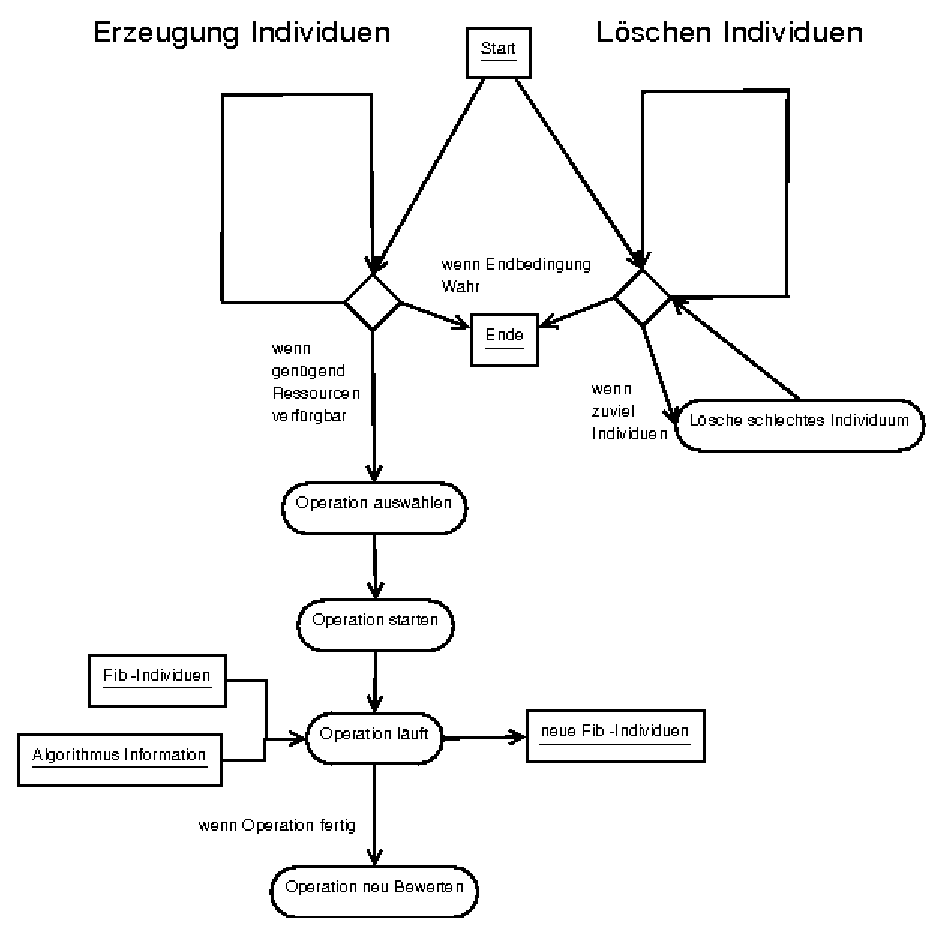
\includegraphics[scale=0.4]{algorithmus}
\end{center}
\caption{Ablaufskizze des genetischen Algorithmus}
\label{figGeneticAlgorithmus}
\end{figure}


Im Nachfolgenden werden die einzelnen Fib-Objekte als Individuen bezeichnet. Die Menge aller Individuen, die zu einem Zeitpunkt im Algorithmus vorhanden sind, wird kurz als Population bezeichnet.


\section{Kernalgorithmus}\index{Kernalgorithmus}

Der Kernalgorithmus nutzt die Bewerter und die Operatoren, um den genetischen Algorithmus zu realisieren. Er soll m"oglichst einfach gehalten und flexibel sein.

Die Bewerter f"ur Individuen oder Operatoren sind ("uber Parameter) austauschbar.

\bigskip
Der Kernalgorithmus beinhaltet einmal die Hauptschleife des genetischen Algorithmus, in dem die Operatoren aufgerufen und Individuen erzeugt werden.

Als zweite Schleife existiert im Algorithmus die Selektionsschleife. Durch sie werden Individuen gel"oscht.

\bigskip
Des Weiteren stellt der Kernalgorithmus Funktionen f"ur die Operatoren bereit. Die Operatoren werden vom Kernalgorithmus "uber eine Methode aufgerufen, die f"ur alle Operatoren gleich ist. Danach holen sich die Operatoren "uber Funktionen des Kernalgorithmus spezifische Werte aus dem Algorithmus, wie z. B. die Individuen, auf denen die Operationen arbeiten. Auf diese Weise sehen die Operatoren f"ur den Kernalgorithmus immer jeweils gleich aus, und er ben"otigt keine Logik speziell f"ur einen bestimmten Operator. Damit werden auch zuk"unftige Anpassungen der Operatoren vereinfacht, da nicht die Schnittstelle aller Operatoren angepasst werden muss, sondern nur die Funktionen, welche der Kernalgorithmus bereitstellt.

Die Aufrufmethode f"ur die Operatoren soll flexibel sein, so dass auch Operatoren nebenl"aufig gestartet werden k"onnen und nicht auf die Beendigung jedes Operatoraufrufs gewartet werden muss. Die Operatoren sollten getrennt vom Kernalgorithmus laufen und diesen nur "uber die vorgegebene Schnittstelle beeinflussen k"onnen. Ein fehlerhafter Operator soll also nicht zu Fehlern im oder zur Beendigung des Gesamtsystems f"uhren.


\section{Bewerten von Individuen}\index{Bewerter!Individuen}\index{Individual!Bewerter}

Der konkrete Bewertungsalgorithmus sollte einfach auszutauschen sein, um verschiedenen Problemstellungen Rechnung tragen zu k"onnen. Der jeweilige Bewertungsalgorithmus wird zur Berechnung der Fitness eines Individuums ben"otigt.

"Uber Parameter f"ur spezielle Bewerter k"onnen diese weiter angepasst werden (beispielsweise damit eingestellt werden kann, wie wichtig eine geringe Gr"o"se gegen"uber eine schnellen Auswertung von Individuen ist).


\subsection{Die Fitness eines Individuums}\index{Fitness!Individuen}\index{Individual!Fitness}

Die Fitness eines Individuums ist durch verschiedene Fitnessfaktoren gegeben.

Einer der wichtigsten ist, inwieweit das Individuum den gew"unschten Originalmultimediadaten (z. B. dem Originalbild) "ahnelt. Je mehr das Individuum (bzw. der Ph"anotyp dessen) den Originalmultimediadaten "ahnelt, umso h"oher sollte die Fitness sein und umso geringer ist der Fehler, den das Individuum f"ur die Darstellung der Originalmultimediadaten macht.

Dieser Fehler (und damit die Fitness des Individuums) kann z. B. "uber die Summe der (quadratischen) Abweichungen (nicht definierte Punkte liefern einen maximalen Fehler) in den Farben zu einem Punkt zwischen dem Originalbild und dem vom Individuum erzeugten Bild bestimmt werden oder "uber ein anderes selbstbestimmtes Abstandsma"s.

Wenn die Fitness f"ur einzelne Teilobjekte des Individuums bestimmt wird, kann dies z. B. dadurch realisiert werden, dass in die Rechnung nur der Bereich einbezogen wird, der durch das Teilobjekt "uberdeckt wird, ein Rand um diesen Bereich noch mit einbezogen wird, oder auch nur das kleinste Quadrat benutzt wird, das dieses Objekt umschlie"st.

Ein anderer sinnvoller Fitnessfaktor ist die Gr"o"se (steigt mit der Anzahl der Elemente) der einzelnen Individuen, um gr"o"seren Individuen eine geringere Fitness zu geben als kleineren Individuen, mit dem gleichen Fehler auf den Originalmultimediadaten, und die kleineren Individuen so zu bevorzugen.

Ein weiterer Fitnessfaktor der einbezogen werden kann, ist eine Sch"atzung "uber die Zeit, die f"ur das Individuum zur Berechnung des dargestellten Multimediaobjekts (Ph"anotyp) ben"otigt wird. Damit kann eventuell sogar die Ausf"uhrungsgeschwindigkeit des Algorithmus erh"oht werden.


\subsection{Selektion durch L"oschen von Individuen}\index{Selektion}

Um die Ressourcen (Arbeitspeicher, Rechenzeit) zu schonen, ist es notwendig, die Anzahl der Individuen (Fib-Objekte) im Bearbeitungsprozess (Individuen die noch am genetischen Algorithmus teilnehmen) zu beschr"anken. Deshalb m"ussen Individuen aus diesem (nach Bedarf) entfernt werden. Dabei sind Individuen mit einer niedrigen Fitness zu bevorzugen.

Deshalb gibt es f"ur den Algorithmus einen \textbf{Mortalit"atsbewerter}\index{Mortalit"atsbewerter}. Dieser bestimmt, mit welcher Wahrscheinlichkeit ein Individuen gel"oscht wird. Um Individuen zu l"oschen, gibt es im Algorithmus eine seperate Schleife, in der gepr"uft wird, ob die maximale Anzahl von Individuen "uberschritten ist. Wenn dies der Fall ist, werden so viele Individuen gel"oscht, bis die maximale Anzahl von Individuen wieder eingehalten wird. Dabei haben Individuen mit einer hohen Bewertung durch den Mortalit"atsbewerter auch eine hohe Wahrscheinlichkeit, gel"oscht zu werden.

Der Mortalit"atsbewerter orientiert sich f"ur seine Bewertung an der Fitness der Individuen. Er kann allerdings durch andere Mortalit"atsbewerter ausgetauscht oder durch Parameter gesteuert werden. Es ist beispielsweise auch m"oglich, einige Individuen als unsterblich bzw. nicht l"oschbar zu deklarieren. Indem z. B. die $n$ ($n>0$) besten Individuen als unsterblich deklariert werden, kann vermieden werden, dass diese gel"oscht werden und somit eines der besten Individuen verloren geht.

Der Mortalit"atsbewerter kann weiterhin "uber die Operatorschnittstelle auf Statusinformationen des Algorithmus zugreifen, um z. B. die Anzahl der bisher erzeugten Individuen zu ermitteln.


\section{Bewerter f"ur Operatoren}\index{Bewerter!Operatoren}

Um zu bestimmen, welcher Operator als n"achstes ausgew"ahlt wird, sind diese zu bewerten. Operatoren, die besser in einer Situation bewertet werden, haben eine h"ohere Wahrscheinlichkeit, in einer "ahnlichen Situation ausgew"ahlt bzw. ausgef"uhrt zu werden.

\bigskip\noindent
Die Situation kann umfassen:
\begin{itemize}
 \item die wievielte Operation bzw. Interaktion ausgef"uhrt wird.
 \item welcher Art das Originalmultimediaobjekt ist ("uber die Definitionen f"ur die Umgebung in den root-Elementen dieses):
 \begin{itemize}
  \item es enth"alt Farben 
  \item es ist Schwarz/Wei"s
  \item es enth"alt Ton
  \item es handelt sich um einen Film
  \item ...
 \end{itemize}
 \item die durchschnittliche (relative) Fitness der Individuen.
 \item die Fitness des besten/schlechtesten Individuums.
 \item die Standardabweichung der Fitnesswerte in der Population.
 \item die Anzahl der Individuen.
 \item Operationen, die bisher angewendet wurden.
 \item ...
\end{itemize}

Der spezielle Bewertungsalgorithmus kann ausgew"ahlt werden. So k"onnen verschiedene Bewertungsalgorithmen leicht gegeneinander ausgetauscht und verglichen werden.

Zur Bewertung der Operatoren werden (von einzelnen Bewertern) eventuell Daten "uber ihre bisherigen Anwendungen permanent gehalten. Auf diese Weise kann der Algorithmus aus vorhergehenden Operatoraufrufen lernen.

Die Bewertung der Operatoren sollte m"oglichst Systemunabh"angig erfolgen, also unabh"angig vom Rechner, auf dem der Algorithmus gerade l"auft.

\bigskip\noindent
Die Bewertungskriterien k"onnen sein:
\begin{itemize}
 \item Ausf"uhrungszeit der Operation
 \item erreichte Verschlechterungen oder Verbesserungen
 \item Zuverl"assigkeit des Operators (Gibt er immer ein Ergebnis zur"uck? St"urzt er manchmal ab?)
 \item ...
\end{itemize}


\section{Die genetischen Operationen auf Fib}

Die Operatoren sind vom genetischen Algorithmus getrennt zu sehen. Es sollte m"oglich sein, beliebig viele Operatoren zum genetischen Algorithmus hinzuzuf"ugen, ohne diesen anpassen zu m"ussen.

Jeder Operator hat eine eindeutige Kennung bzw. ID, "uber die ihm zugeh"orige Werte (z. B. seine bisherige Performance) zugeordnet werden k"onnen.

Wird ein Operator ausgef"uhrt, ist dies eine Operation.

Diese Operationen sind dazu gedacht, Kodierungsalgorithmen zu implementieren. Operatoren sollten also nicht m"oglichst einfach sein, sondern k"onnen durchaus komplexe Algorithmen beinhalten.

Die Operatoren sollen auch m"oglichst zahlhaft sein, und der Algorithmus ist f"ur die Auswahl guter Operatoren verantwortlich. Daher ist es auch erw"unscht, mit sinvollen Teilen von Operatoren eigene Operatoren zu erstellen. Dabei sollten sowohl die Originaloperatoren als auch der Operator, der den extrahierten Teil enth"alt, im Algorithmus verbleiben.

F"ur Spezialanwendungen kann ein genetischer Algorithmus verwendet werden, dessen Menge der Operatoren auf die n"utzlichsten f"ur diese Anwendung eingeschr"ankt wurde.
Auch k"onnen f"ur eine Anwendung n"utzliche Operatoren zu einem (nicht genetischen) Algorithmus kombinert werden, der diese in determinerter Weise verbindet.


\subsection{Vermehrung}

Bei der ``Vermehrung'' wird im Allgemeinen ein Individuum aus der Population genommen, bevorzugt Individuen mit hoher Fitness, dieses kopiert und durch eine Operation ver"andert. Ist das entstehende Individuum ein ``neues'' Objekt (wenn es kein gleiches in der Population gibt), wird es zur Menge hinzugenommen. Es k"onnen auch bereits vorhandene Individuen "ubernommen werden.

Im Algorithmus wird die Vermehrung dadurch realisiert, dass eine Operation ausgef"uhrt wird. Diese Operation holt sich dann "uber die Operationenschnittstelle vom Algorithmus alle ben"otigten Daten. Zu den ben"otigten Daten k"onnen ein oder mehrere Individuen geh"oren oder Daten "uber den bisherigen Verlauf des Algorithmus (z. B. die Nummer der bisherigen Interaktionen bzw. Operationen).


\section{Der soziale Aspekt des genetische Algorithmus}\index{Algorithmus!Sozialkomponente}

Die strikte Trennung der Operatoren vom Algorithmus und die M"oglichkeit, Operationen leicht hinzuf"ugen zu k"onnen, hat seinen Grund in eher sozialen "Uberlegungen.

Normale Kodierungsalgorithmen beschr"anken sich bei den Kodierungsmethoden auf eine oder nur wenige Ideen von einigen (in der Gr"o"senordnung von 1 bis 100) Menschen (dem Entwicklerteam). Da es aber viel mehr (in der Gr"o"senordnung von wahrscheinlich 100000) Menschen weltweit gibt, die sich im weiteren Sinne mit der effizenten Kodierung von Multimediaobjekten besch"aftigen, bleiben dadurch zwangsl"aufig auch viele Ideen zur Kodierung unber"ucksichtigt. Selbst wenn ein Teil dieser Menschen daran Interesse hat, ihre Ideen einzubringen, ist dies nur sehr schwer bis unm"oglich zu realisieren.

In den Fib-Algorithmus kann aber jeder neue Ideen in Form neuer Operatoren einbringen (ein Begriff daf"ur ist ``Crowdsourcing''). Daf"ur sind lediglich ausreichende Kenntnisse der Fib-Multi\-media\-beschrei\-bungs\-sprache und der Schnittstelle des Algorithmus f"ur die Operatoren n"otig. Um neue Ideen bzw. Operatoren zur effizenten Kodierung von Multimediaobjekten einzubringen, sollten keine Anpassungen am Algorithmus oder anderen Operatoren n"otig sein. Dadurch werden Seiteneffekte beschr"ankt und jede Implementierung einer Idee hat sich nur um die Idee bzw. deren Operator zu k"ummern. Es sind also keine weiteren Kenntnisse des Algorithmus oder gar anderer Operatoren von N"oten. Auf diese Weise kann das System wachsen, ohne dass sich die Komplexit"at des (Kern-)Systems vergr"o"sert und die Wartung und Erweiterung des Systems schwieriger wird.

Der Algorithmus und die Bildbeschreibungssprache sollten so angelegt sein, dass sich auch Laien ohne gr"o"seren Aufwand einarbeiten und neue Ideen bzw. Operatoren realisieren k"onnen. Insbesondere sollten Studenten und Studierende (z. B. Menschen mit Informatik als Hobby) der Informatik, sich innerhalb weniger Tage soweit einarbeiten k"onnen, dass sie einen eigenen Operator realisieren und einbinden k"onnen. (Wie n"utzlich oder effizient dieser ist, sei erst einmal dahingestellt.)

Die GNU-GPL-Lizenz, unter dem der Algorithmus steht, kl"art die rechtliche Situation, unter der neue Operatoren stehen. Dadurch k"onnen neue Operatoren legal eingebunden werden, solange nicht andere Rechte verletzt werden (eine Verletzung w"are beispielsweise, dass in den Operatoren verwendete Algorithmen oder Codes unter inkompatiblen Lizenzen stehen). Neue Operatoren k"onnen auch der Allgemeinheit zur Verf"ugung gestellt werden.

Die Bewertung der Operatoren sollte motivieren, eigene Operatoren einzubinden. Dadurch kann jeder, der einen Operator hinzugef"ugt hat, realistisch einsch"atzen, wie gut sein Operator sich im Verh"altnis zu anderen Operatoren in einer Situation macht. Der Wettbewerb unter Operatorenautoren sollte f"ur neue bessere Operatoren f"orderlich sein.


All dies sollte dazu f"uhren, dass nicht nur ein kleines Entwicklerteam zur Verbesserung der Kodierung von Fib-Objekten beitr"agt, sondern dass ein viel gr"o"serer Kreis von Menschen sich mit diesen Thema besch"aftigt. Dies sollte der Entwicklung und Verbreitung von Fib einen weiteren Schub geben.

In diesem Sinne ist der genetische Algorithmus f"ur Fib ein transgenialer Algorithmus, der darauf angelegt ist, die Ideen von Menschen zur Kodierung von Multimediadaten aus deren K"opfen herauszuholen und in einem Topf zu transportieren/sammeln. Damit sollen diese Ideen/Algorithmen mehr leisten k"onnen, als sie es einzeln k"onnten. Der Algorithmus kann damit mehr Intelligenz in sich vereinen, als es ein Mensch (oder auch eine kleine Gruppe) hervorbringen kann.


\section{Warum sich genetische Algorithmen zur Multimediakodierung anbieten}

Es gibt im Allgemeinen keinen Algorithmus der Rastergrafiken direkt in speicherschonende Vektorbilder umwandeln kann, bei denen die St"arken der entsprechenden Vektorbeschreibungssprache wirklich genutzt werden. F"ur die Umwandlung von einem Multimediaformat in ein anderes ergibt sich oft eine "ahnliche Problematik, insbesondere wenn das erste Multimediaformat die Eigenschaften von Punkten eines euklidischen (diskreten) Raumes direkt angibt (z. B. um Aufnahmen direkt abspeichern zu k"onnen) und das zweite Multimediaformat komplexe Objekte (z. B. Rechtecke oder/und Kreise) in Multimediaobjekten kodiert.

Da ein genetischer Algorithmus das Potential hat, alle m"oglichen Beschreibungen einer Multimediasprache zu generieren und unter diesen nat"urlich auch gute Beschreibungen sind, welche die St"arken der Multimediasprache in Bezug auf das Originalobjekt nutzen, hat ein genetischer Algorithmus nat"urlich auch das Potential, gute Beschreibungen zu generieren. Wenn im genetischen Algorithmus vorhandenes Wissen gut eingebaut wurde, kann er gute Beschreibungen wahrscheinlich auch schneller finden als eine reine Zufallssuche.

Noch ein weiterer Vorteil von genetischen Algorithmen ist die gro"se Freiheit bei der Wahl der Problembeschreibung (Multimediasprache) und der m"oglichen Operatoren auf dieser. So kann v"ollig frei eine Multimediasprache nach eigenen Vorstellungen entworfen werden, die bestimmte Eigenschaften hat, z. B. Lesbarkeit, Einfachheit. Bei den Operatoren kann beliebig viel Wissen eingebaut werden. So ist es unter anderem auch m"oglich, schon bekannte gute Algorithmen zur "Ubersetzung von Rastergrafiken in Vektorbilder oder Teile von ihnen in Operatoren zu verwenden, so dass der genetische Algorithmus auf Rastergrafiken vom Ergebnis her mindestens so gut wird wie der verwendete Algorithmus, aber noch bessere Ergebnisse erzeugen kann.

Der gro"se Nachteil von genetischen Algorithmen, dass sie sehr viel Zeit oder Rechenaufwand ben"otigen, wird dadurch abgeschw"acht, dass dieser anf"anglich hohe Aufwand ``billig'' sein kann und sich sp"ater auszahlt. Der genetische Algorithmus kann z. B. als Hintergrundprozess mit niedriger Priorit"at laufen, so dass er nur "uberfl"ussige Rechnerleistung verbraucht. Sp"ater kann durch das Ergebnis, das er geliefert hat, viel "Ubertragungsbandbreite eingespart werden.

Dies alles spricht f"ur den Versuch, genetische Algorithmen zur Multimediakodierung zu verwenden.


\section{Komplexit"atsabsch"atzung}
\label{abschaet}

Mit dem Ansatz aus Abschnitt \ref{secPowerOfFibOnPictures} auf Seite \pageref{secPowerOfFibOnPictures} kann eine beliebiges Rastergrafik in ein Fib-Objekt konvertiert werden, wobei der Kodierungsaufwand linear mit der Anzahl der Punkte und Eigenschaften w"achst, da jeder Punkt mit seinen Eigenschaften einfach in ein Listenelement eingef"ugt werden kann und die Erzeugung der sonstigen Fib-Elemente (des root-Elements) konstante Zeit ben"otigt.

Dieser Ansatz ist auf beliebige Multimediadaten erweiterbar, die als Eigenschaften von Punkten eines endlichen, euklidischen, diskreten Raumes darstellbar sind. So kann immer ein Operator konstruiert werden, der ein Multimediaobjekt in linearer Zeit mit der Anzahl der Punkte und Eigenschaften in ein entsprechendes Fib-Objekt umwandelt. Dieses Fib-Objekt w"achst auch von der Gr"o"se her nur linear mit der Anzahl der Punkte und Eigenschaften des Originalmultimediaobjekts.
Dieser Operator erzeugt allerdings keine effiziente Fib-Objektdarstellung, da er nicht die M"oglichkeiten von Fib nutzt.

Wieviel Aufwand die Erzeugung besserer Fib-Objekte ben"otigt, kann nur schwer abgesch"atzt werden, da sowohl die Operatoren als auch die Multimediaobjekte beliebig sein k"onnen. Es kann aber davon ausgegangen werden, dass f"ur Multimediaobjekte mit einfacheren Strukturen der Aufwand auch geringer ist.


\section{Parallelen zur nat"urlichen Evolution}

Als Parallele seien hier die Bakterienst"amme (z. B. E. coli) aufgef"uhrt. Sie besitzen Gene, aufgrund derer bei ihnen genetische Evolution auftritt.

Bei diesen Bakterienst"ammen (z. B. E. coli) kann es auch zu einem Gentransfer kommen, dabei wird ein Teil der Geninformationen (des Genmaterials oder dessen Kopien) von einer Bakterie zu einer anderen "ubertragen. Daneben gibt es nat"urlich auch Mutationsprozesse.

Ein Fib-Objekt kann als Information betrachtet werden, die ein Multimediaobjekt kodiert, so wie Bakteriengene eine Bakterie kodieren (Aufbau und Verhalten).

Die einzelnen Fib-Elemente sind dabei weniger als die Basen der Gene zu sehen, sondern vielmehr als die Funktionalit"at von Genen oder Genmengen. So wie bei den Bakterien durch Kombination der Gene bzw. der Dinge, die sie kodieren (z. B. Enzyme), erst komplexere Funktionalit"aten definiert werden (z. B. Umsetzung von Zucker in Bewegungsenergie), entstehen bei Fib-Objekten erst durch Kombination der Elemente (Teil-)Multimediaobjekte (z. B. [Teil-]Bilder).

Fib-Teilobjekte k"onnen auch, wie beim Gentransfer bei den Bakterien, in andere Fib-Objekte "ubertragen werden und unterliegen einer Mutation, wobei auch bei den Bakterien schwer zu sagen ist, ob die Mutation der Gene wirklich v"ollig zuf"allig ist oder ob im Laufe der Jahrmillionen nicht Mechanismen entstanden sind, die zu einer ``intelligenteren'' Mutation f"uhren, bzw. worin das zuf"allige Element besteht. Einzelne Fib-Objekte k"onnen dabei nicht nur als einzelne Bakterien angesehen werden, sondern auch als alle Bakterien mit identischen Geninformationen.

Das Originalmultimediaobjekt stellt die Nische dar, an welche sich die Fib-Objekte (Bakterien) anpassen sollen. Sie k"onnen dies auf viele unterschiedliche Arten tun, und die Anpassung muss auch nicht perfekt sein.

Allerdings werden beim genetischen Algorithmus f"ur Fib-Objekte Operatoren angestrebt, die gezielte Verbesserungen vornehmen. Ein solcher explizit gerichteter Mechanismus ist bei Bakterien nicht zu erwarten.

F"ur weitere Informationen zur Genetik bei Bakterien sei auf ``Einf"uhrung in die Mikrobiologie''(\cite{genTrans}) verwiesen. Ein gutes Buch zur Evolution im allgemeinen ist ``Die L"osung von Darwins Dilemma'' \cite{LDD_2007} .
















%TODO
%
% Copyright (c) 2008  Betti "Osterholz
%
% Permission is granted to copy, distribute and/or modify this document
% under the terms of the GNU Free Documentation License, Version 1.2 or
% any later version published by the Free Software Foundation;
% with no Invariant Sections, no Front-Cover Texts, and no Back-Cover Texts.
%
% A copy of the license is included in the file ``fdl.tex'' .
%
% The file contains the documentation for the fib-storage formats.
%

\newpage
\part{Fib-Dateiformate}
\label{partFileFormat}

In diesen Abschnitt werden die Speicherformate vorgestellt, in denen vollst"andige Fib-Objekte abgespeichert werden. Davon gibt es zwei: ein Format zum m"oglichst komprimierten Abspeichern (siehe Abschnitt \ref{fibCompressing} auf Seiet \pageref{fibCompressing}) und ein Format, um ein Fib-Objekt gut lesbar als XML-Struktur darzustellen (siehe Abschnitt \ref{xmlFormat} auf Seiet \pageref{xmlFormat}).


\section{Komprimierte Fib-Daten}\index{Komprimierung}\index{Format!komprimiert}
\label{fibCompressing}

Da eine Speicherplatz sparende Repr"asentation eines der Hauptziele der Fib-Multi\-media\-be\-schrei\-bungs\-sprache ist, sollten die Fib-Elemente mit m"oglichst wenig Bits bzw. Bytes gespeichert werden k"onnen. Daf"ur wird hier ein komprimierendes Speicherformat definiert. Es wird kein Standardkomprimierungsalgorithmus verwendet, da dieser keine R"ucksicht auf Besonderheiten der Fib-Multimedia\-be\-schrei\-bungs\-sprache nehmen w"urde.

%Die Struktur der komprimierten Daten entspricht weitesgehend der Struktur des XML-Formats, siehe \ref{xmlFormat}.

Die Darstellung von \textbf{ganzen Zahlen} erfolgt im Zweierkomplement System (auch 2-Komplement, Zweikomplement, Basiskomplement, K2-Zahl, 2K-Zahl, two's complement). F"ur \textbf{nat"urliche Zahlen} (inklusive der $0$) wird das Dualsystem verwendet. Die Anzahl der Bits von Vektorelementen oder Variablen wird jeweils durch den entsprechenden Definitionsbereich bestimmt (z. B. f"ur Zahlen f"ur die horizontale Dimension oder einen Grauwert) oder fest vorgegeben (z. B. f"ur Zahlen f"ur das Byte Offset in den root-Elementen).

%endianess


\textbf{Reelle Zahlen} werden als Gleitkommazahlen (auch Flie"skommazahl engl. floating point number) dargestellt. Die Anzahl der Bits f"ur den Exponenten und die Mantisse werden durch die jeweilige Definitionsbereichsdefinition angegeben.

Die Zahlen werden im Little Endian Format gespeichert.

Alle \textbf{Texte} werden in Unicode kodiert.


F"ur die nachfolgende Beschreibung ist leider die \textbf{Schreibweise von Bits} nicht so einfach umzusetzen. In der normalen Schreibweise werden Zahlen von rechts nach links, Texte allerdings von links nach rechts geschrieben. Dies f"uhrt dazu, dass kurze Bitfolgen, so wie sie in einem Byte auftauchen, eher wie Zahlen von rechts nach links geschrieben werden. Wenn die Bitfolgen allerdings l"anger werden bzw. wenn Bits in einer Datei oder einem Datenstrom betrachtet werden, ist die Schreibweise wie in Texten von links nach rechts eher angebracht. Ansonsten, wenn die Zahlenschreibweise angewendet wird, steht am Ende einer langen Zeile von Bits das erste Bit aus der Datei.

Im Nachfolgenden werden deshalb die Bits einzelner Elemente wie Zahlen von von rechts nach links geschrieben, da diese Bitfolgen meist kurz sind. Einzelne Elemente werden am Computer auch meist im Hexadezimalsystem angezeigt und verarbeitet, welches auch wie Zahlen von rechts nach links arbeitet. Die umgekehrte Schreibweise w"urde die Arbeit mit den komprimierten Elementen nur erschweren. Die Bits einzelner Bytes werden meistens der "Ubersichtlichkeit halber mit einem Semikolon (';') getrennt.

Wenn allerdings ein Datenstrom aus mehreren Elementen dargestellt wird, sind die Bits wie bei Texten von links nach rechts angeordnet. Dies f"uhrt leider dazu, dass die Bits der einzelnen Elemente in umgekehrter Reihenfolge dargestellt werden.

%9 Fib-Elemente plus root

\subsection{Dateiheader}

Jede komprimierte Fib-Datenstrom beginnt mit den drei Buchstaben ``fib''. Die Dateiendung f"ur komprimierte Fib-Dateien sollte ``.fib'' sein.


\subsection{Root-Element}\index{root-Element|(}
\label{secCompressedRootElement}

Zur Beschreibung des root-elements siehe Abschnitt \ref{fibRootElement} auf Seite \pageref{fibRootElement} .

Das Fib-root-Element braucht keine separate Einleitung. Die Daten des obersten root-Elements beginnen mit dem dritten Byte (die Z"ahlung beginnt bei 0) direkt nach der Datenstromeinleitung ``fib''. Andere root-Elemente folgen auf ihren Identifier.

\bigskip\noindent
F"ur das root-Element werden nacheinander folgende Felder geschrieben (dabei wird jedes Element jeweils fals n"otig auf ein volles Byte mit $0$ aufgef"ullt):
\begin{enumerate}
 \item 16-Bit-Feld zur Angabe der optionalen Informationsfelder (siehe Abschnitt \ref{secCompressedOptionlInfos})
 \item 64-Bit-Feld zur Angabe weiterer optionaler Informationsfelder (siehe Abschnitt \ref{secCompressedOptionlInfos}); nur vorhanden, wenn Bit 16 der optionalen Informationsfelder gesetzt ist
 \item ein 144($=16+64+64$)-Bit-Feld f"ur die Checksumme (siehe Abschnitt \ref{secCompressedRootChecksumm} auf Seite \pageref{secCompressedRootChecksumm} ); nur vorhanden, wenn Bit 1 der optionalen Informationsfelder gesetzt ist
 \item Nummer des Bytes des root-Objekts (Offset), ab dem die Definitionsbereiche ($Domains$ und $DomainsValues$) definiert werden; nur vorhanden, wenn Bit 3 der optionalen Informationsfelder gesetzt ist
 \item Nummer des Bytes des root-Objekts (Offset), ab dem die Eingabevariablen definiert werden; nur vorhanden, wenn Bit 4 der optionalen Informationsfelder gesetzt ist
 \item Nummer des Bytes des root-Objekts (Offset), ab dem das Haupt-Fib-Objekt definiert wird
 \item Nummer des Bytes des root-Objekts (Offset), ab dem die weiteren root-Objekte definiert werden; nur vorhanden, wenn Bit 6 der optionalen Informationsfelder gesetzt ist
 \item Nummer des Bytes des root-Objekts (Offset), ab dem die Identifier von verwendeten Datenbankobjekten aufgelistet werden; nur vorhanden, wenn Bit 7 der optionalen Informationsfelder gesetzt ist
 \item Nummer des Bytes des root-Objekts (Offset), ab dem der optionale Teil (Optionalpart) kommt; nur vorhanden, wenn Bit 8 der optionalen Informationsfelder gesetzt ist
 \item Nummer des Bytes des root-Objekts (Offset), ab dem das root-Objekt zu Ende ist, bzw. Anzahl der Bytes, welche das root-Objekt lang ist
 \item Multimediainformationen (siehe Abschnitt \ref{secCompressedMultimediainfo} auf Seite \pageref{secCompressedMultimediainfo}); nur vorhanden, wenn Bit 2 der optionalen Informationsfelder gesetzt ist
 \item Definitionsbereiche (siehe Abschnitt \ref{secCompressedDefinitionranges} auf Seite \pageref{secCompressedDefinitionranges}); nur vorhanden, wenn Bit 3 der optionalen Informationsfelder gesetzt ist
 \item Eingabevariablen (siehe Abschnitt \ref{secCompressedRootInputVar} auf Seite \pageref{secCompressedRootInputVar}); nur vorhanden, wenn Bit 4 der optionalen Informationsfelder gesetzt ist
 \item Haupt-Fib-Objekt (siehe Abschnitt \ref{secCompressedRootMainObject} auf Seite \pageref{secCompressedRootMainObject})
 \item weitere root-Objekte (siehe Abschnitt \ref{secCompressedRootSubRoot} auf Seite \pageref{secCompressedRootSubRoot}); nur vorhanden, wenn Bit 6 der optionalen Informationsfelder gesetzt ist
 \item Identifier von verwendeten Datenbankobjekten (siehe Abschnitt \ref{secCompressedRootDBIdentifier} auf Seite \pageref{secCompressedRootDBIdentifier}); nur vorhanden, wenn Bit 7 der optionalen Informationsfelder gesetzt ist
\item der optionale Teil (siehe Abschnitt \ref{secCompressedRootOptionalPart} auf Seite \pageref{secCompressedRootOptionalPart}); nur vorhanden, wenn Bit 8 der optionalen Informationsfelder gesetzt ist
\end{enumerate}

Wenn ein einzelnes Bit in den optionalen Informationsfeldern f"ur ein Feld nicht gesetzt ist, entf"allt diese Feld.

F"ur die Felder mit der ``Nummer des Bytes des root-Elements (Offset)'' werden jeweils 8 Byte oder 64 Bit verwendet. Die Zahl im Feld geh"ort zu den nat"urlichen Zahlen. Angegeben wird jeweils die Nummer des Bytes ab Anfang des root-Elements, ab dem das entsprechende Element beginnt (also f"ur das erste Byte des Elements). Die Z"ahlung der Bytes im root-Element beginnt bei 0. Das optionale Informationsfeld hat also den Offset 0.

Alle Texte, die nicht im optionalen Teil stehen, werden in den optionalen Teil ausgelagert (siehe Abschnitt \ref{secCompressedRootOptionalPart} auf Seite \pageref{secCompressedRootOptionalPart}).


\subsubsection{Optionale Informationsfelder}
\label{secCompressedOptionlInfos}

An dieser Stelle steht ein 16-Bit-Feld, dessen Bits das Vorhandensein von optionalen Informationsfeldern im root-Element anzeigt.

\bigskip\noindent
Dabei schalten die einzelnen Bits (die Z"ahlung beginnt bei 1) die folgenden Informationsfelder:
\begin{itemize}
 \item [1] Checksumme (siehe Abschnitt \ref{secCompressedRootChecksumm} auf Seite \pageref{secCompressedRootChecksumm})
 \item [2] Multimediainformationen (siehe Abschnitt \ref{secCompressedMultimediainfo} auf Seite \pageref{secCompressedMultimediainfo})
 \item [3] Definitionsbereiche (siehe Abschnitt \ref{secCompressedDefinitionranges} auf Seite \pageref{secCompressedDefinitionranges})
 \item [4] Eingabevariablen (siehe Abschnitt \ref{secCompressedRootInputVar} auf Seite \pageref{secCompressedRootInputVar})
 \item [5] frei
 \item [6] weitere root-Objekte (siehe Abschnitt \ref{secCompressedRootSubRoot} auf Seite \pageref{secCompressedRootSubRoot})
 \item [7] Identifier von verwendeten Datenbankobjekten (siehe Abschnitt \ref{secCompressedRootDBIdentifier} auf Seite \pageref{secCompressedRootDBIdentifier})
 \item [8] optionaler Teil (siehe Abschnitt \ref{secCompressedRootOptionalPart} auf Seite \pageref{secCompressedRootOptionalPart})
 \item 9 bis 15 Bits sind noch nicht belegt und stehen f"ur zuk"unftige Belegungen zur Verf"ugung
 \item [16] weitere optionale Felder, angegeben durch ein folgendes 64-Bit-Feld f"ur weitere optionale Informationsfelder
\end{itemize}

Im Nachfolgenden werden die einzelnen Bits, wann sie eingesetzt werden und ihre Auswirkung beschrieben.


\paragraph{1. Checksummenbit}

\ \\\\\noindent
\textbf{Gesetzt wenn:} Ein Checksummenfeld im root-Element existiert.

\bigskip\noindent
\textbf{Auswirkungen wenn gesetzt:}
Ein Checksummenfeld (siehe Abschnitt \ref{secCompressedRootChecksumm} auf Seite \pageref{secCompressedRootChecksumm}) ist vorhanden.

\bigskip\noindent
\textbf{Nicht gesetzt wenn:} Es existiert kein Checksummenfeld im root-Element.

\bigskip\noindent
\textbf{Auswirkungen wenn nicht gesetzt:}
Ein Checksummenfeld ist nicht vorhanden.


\paragraph{2. Multimediainformationenbit}

\ \\\\\noindent
\textbf{Gesetzt wenn:} F"ur das aktuelle root-Element existieren Multimediainformationen, welche von den ererbten Multimediainformationen abweichen. Dabei werden Multimediainformationen eines root-Elements jeweils an in diesem enthaltende root-Elemente vererbt, wenn die enthaltenden root-Elemente nicht selbst (irgendwelche) abweichende Multimediainformationen definieren.
%TODO Olli: Bitte "`eindeutschen"': "`... an in diesem enthaltende root-Elemente vererbt,..."' (vorheriger Satz)

\bigskip\noindent
\textbf{Auswirkungen wenn gesetzt:}
Es werden die Multimediainformationen f"ur das aktuelle root-Element angegeben (siehe Abschnitt \ref{secCompressedMultimediainfo} auf Seite \pageref{secCompressedMultimediainfo}).

\bigskip\noindent
\textbf{Nicht gesetzt wenn:} Die Multimediainformationen entsprechen den ererbten Multimediainformationen.

Im obersten root-Element (bzw. in einem root-Element, das in keinem anderen root-Element vorhanden ist) muss das Bit immer gesetzt sein und damit die Multimediainformationen vorhanden sein.

\bigskip\noindent
\textbf{Auswirkungen wenn nicht gesetzt:}
Es werden keine Multimediainformationen f"ur das aktuelle root-Element angegeben. Die g"ultigen Multimediainformationen f"ur das root-Element werden von dem root-Element, in dem es vorhanden ist, ererbt.


\paragraph{3. Definitionsbereiche}

\ \\\\\noindent
\textbf{Gesetzt wenn:} F"ur das aktuelle root-Element existieren Definitionsbereiche.

\bigskip\noindent
\textbf{Auswirkungen wenn gesetzt:}
Es werden die Definitionsbereiche f"ur das aktuelle root-Element ausgegeben (siehe Abschnitt \ref{secCompressedDefinitionranges} auf Seite \pageref{secCompressedDefinitionranges}) und der Offset, wann diese im root-Element beginnen.

\bigskip\noindent
\textbf{Nicht gesetzt wenn:} F"ur das aktuelle root-Element existieren keine Definitionsbereiche.

\bigskip\noindent
\textbf{Auswirkungen wenn nicht gesetzt:}
Es wird kein Offset ausgegeben, wann die Angabe der Definitionsbereiche im root-Element beginnt, und es werden keine Definitionsbereiche f"ur das aktuelle root-Element angegeben.


\paragraph{4. Eingabevariablen}

\ \\\\\noindent
\textbf{Gesetzt wenn:} F"ur das aktuelle root-Element existieren Eingabevariablen.

\bigskip\noindent
\textbf{Auswirkungen wenn gesetzt:}
Es werden die Eingabevariablen f"ur das aktuelle root-Element angegeben (siehe Abschnitt \ref{secCompressedRootInputVar} auf Seite \pageref{secCompressedRootInputVar}) und der Offset, wann diese im root-Element beginnen.

\bigskip\noindent
\textbf{Nicht gesetzt wenn:} F"ur das aktuelle root-Element existieren keine Eingabevariablen.

\bigskip\noindent
\textbf{Auswirkungen wenn nicht gesetzt:}
Es wird kein Offset ausgegeben, wann die Angabe der Eingabevariablen im root-Element beginnt, und es werden keine Eingabevariablen f"ur das aktuelle root-Element angegeben.


\paragraph{6. weitere root-Objekte}

\ \\\\\noindent
\textbf{Gesetzt wenn:} F"ur das aktuelle root-Element existieren Unter-root-Objekte.

\bigskip\noindent
\textbf{Auswirkungen wenn gesetzt:}
Es werden die Unter-root-Objekte f"ur das aktuelle root-Element angegeben (siehe Abschnitt \ref{secCompressedRootSubRoot} auf Seite \pageref{secCompressedRootSubRoot}) und der Offset, wann diese im root-Element beginnen.

\bigskip\noindent
\textbf{Nicht gesetzt wenn:} F"ur das aktuelle root-Element existieren keine Unter-root-Objekte.

\bigskip\noindent
\textbf{Auswirkungen wenn nicht gesetzt:}
Es wird kein Offset ausgegeben, wann die Angabe der Unter-root-Objekte im root-Element beginnt, und es werden keine Unter-root-Objekte f"ur das aktuelle root-Element angegeben.


\paragraph{7. Identifier von verwendeten Datenbankobjekten}

\ \\\\\noindent
\textbf{Gesetzt wenn:} F"ur das aktuelle root-Element werden Identifier von verwendeten Datenbankobjekten angegeben.

\bigskip\noindent
\textbf{Auswirkungen wenn gesetzt:}
Es werden die Identifier von verwendeten Datenbankobjekten f"ur das aktuelle root-Element angegeben (siehe Abschnitt \ref{secCompressedRootDBIdentifier} auf Seite \pageref{secCompressedRootDBIdentifier}) und der Offset, wann diese im root-Element beginnen.

\bigskip\noindent
\textbf{Nicht gesetzt wenn:} F"ur das aktuelle root-Element existieren keine Identifier von verwendeten Datenbankobjekten.

\bigskip\noindent
\textbf{Auswirkungen wenn nicht gesetzt:}
Es wird kein Offset ausgegeben, wann die Angabe der Identifier von verwendeten Datenbankobjekten im root-Element beginnt, und es werden keine Identifier von verwendeten Datenbankobjekten f"ur das aktuelle root-Element angegeben.


\paragraph{8. optionaler Teil}

\ \\\\\noindent
\textbf{Gesetzt wenn:} F"ur das aktuelle root-Element wird der optionale Teil angegeben.

\bigskip\noindent
\textbf{Auswirkungen wenn gesetzt:}
Es wird der optionale Teil f"ur das aktuelle root-Element angegeben (siehe Abschnitt \ref{secCompressedRootOptionalPart} auf Seite \pageref{secCompressedRootOptionalPart}) und der Offset, wann diese im root-Element beginnen.

\bigskip\noindent
\textbf{Nicht gesetzt wenn:} F"ur das aktuelle root-Element ist kein optionaler Teil vorhanden, weil diese beispielsweise nicht mit abgespeichert wurden.

\bigskip\noindent
\textbf{Auswirkungen wenn nicht gesetzt:}
Es wird kein Offset ausgegeben, wann die Angabe der optionale Informationen im root-Element beginnt, und es werden keine optionalen Informationen f"ur das aktuelle root-Element angegeben.


\paragraph{16. weitere optionale Felder}

\ \\\\\noindent
\textbf{Gesetzt wenn:} 64 weitere optionale Informationsbits sind vorhanden.

\bigskip\noindent
\textbf{Auswirkungen wenn gesetzt:}
Auf dem 16-Bit-Feld zur Bestimmung der vorhandenen optionalen Informationen folgt noch ein weiteres 64-Bit-Feld zur Bestimmung von weiteren optionalen Informationen. Diese Bits sind f"ur zuk"unftige Benutzungen gedacht und werden zur Zeit noch nicht verwendet.

\bigskip\noindent
\textbf{Nicht gesetzt wenn:} Die 64 weiteren optionalen Informationsbits sind nicht vorhanden.

\bigskip\noindent
\textbf{Auswirkungen wenn nicht gesetzt:}
Auf den 16-Bit-Feld folgen keine weiteren Bits zur Anzeige der vorhandenen optionalen Informationen.



\subsubsection{Checksummenfelder}\index{Checksumme}
\label{secCompressedRootChecksumm}

Mit diesem Feld kann auch das root-Element mit einer Checksumme versehen werden.

Das Verfahren entspricht dem der Checksummeneigenschaft aus dem Abschnitt \ref{secCompressedChecksumm} auf Seite \pageref{secCompressedChecksumm}.

An dieser Stelle stehen 3 Parameter, welche eine 16 Bit und zwei 64 Bit nat"urliche Zahlen sind. Der erste Parameter $A$ gibt die Art der Checksumme an. Der zweite Parameter $B$ gibt an, alle wieviel Bits eine Checksumme generiert werden soll und der dritte Parameter $C$, wieviel Bits die Checksumme haben soll. Die Angaben gelten f"ur den Bereich nach den drei Parametern (auch in Unter-root-Elementen). Die Checksumme wird so wie in Abschnitt \ref{secCompressedChecksumm} auf Seite \pageref{secCompressedChecksumm} beschrieben umgesetzt.


\subsubsection{Multimediainformationen}\index{Multimediainformationen}
\label{secCompressedMultimediainfo}

In der Tabelle \ref{tableCompressedMultimediainfo} ist der Aufbau des Multimediainformationsabschnitts eines root-Elements beschrieben.
Die Gr"o"se eines Multimediabschnitts ist $2*64=128$ Bit oder $16$ Byte.

\begin{table}[htbp]
\begin{center}
\begin{tabular}{|p{20mm}|p{7mm}|p{7mm}|p{16mm}|p{70mm}|}\hline
	Element & An\-zahl & Bits & Typ & Beschreibung \\\hline\hline
	Fib-Version & 1 & 64 & nat"urliche Zahl & Die Versionsnummer der Fib-Multimediabeschreibungssprache, die zum Laden des Fib-Objekts ben"otigt wird. Diese Nummer wird mit jeder neuen Version der Fib-Multimediabeschreibungssprache um eins erh"oht. Sie kann zu einer menschenlesbaren Form (z. B. ``Fib V1.2.3'') gemappt werden. Hier wird allerdings nur eine Zahl verwendet, da ansonsten eine bestimmte Form festgelegt w"urde, die nur noch schwer ge"andert werden kann. Es kann eine menschenlesbaren Form der Version im optionalen Teil angegeben werden.\\\hline
	DB-Version & 1 & 64 & nat"urliche Zahl & Die Versionsnummer der Fib-Datenbank, die zum Laden des Fib-Objekts ben"otigt wird. Diese Nummer wird mit jeder neuen Version der Fib-Datenbank um eins erh"oht. Sie kann zu einer menschenlesbaren Form (z. B. ``Fib DB V1.2.3'') gemappt werden. Hier wird allerdings nur eine Zahl verwendet, da ansonsten eine bestimmte Form festgelegt w"urde, die nur noch schwer ge"andert werden kann. Es kann eine menschenlesbaren Form der Version im optionalen Teil angegeben werden.\\\hline
\end{tabular}
\end{center}
\caption{Daten der Multimediainformationen}
\label{tableCompressedMultimediainfo}
\end{table}


\subsubsection{Definitionsbereiche}
\label{secCompressedDefinitionranges}\label{secCompressedDomains}
\index{Speicherplatzliste}\index{Definitionsbereiche}

Der Definitionsbereichsabschnitt besteht aus zwei Listen mit unterschiedlich langen Eintr"agen. Die L"ange der Eintr"age wird von ihrem Inhalt bestimmt.

Der Definitionsbereichsabschnitt wird mit einer 64 Bit nat"urlichen Zahl eingeleitet, welche die Anzahl der Eintr"age f"ur die Definitionsbereichsliste angibt. Danach folgt die Definitionsbereichsliste.

Auf diese wiederum folgt eine 64 Bit nat"urliche Zahl, welche die Anzahl der Elemente in der Speicherplatzliste (die Definitionsbereichen f"ur Werte) angibt, und dann die Speicherplatzliste.

Dabei k"onnen eine oder beide Listen auch leer sein. F"ur leere Listen wird dann entsprechend nur die einleitende 64 Bit nat"urliche Zahl gespeichert, die dann 0 ist

Die Definitionsbereichsliste gibt die Definitionsbereiche der einzelnen Elemente an. Ist ein Wert (z. B. einer Variable) au"serhalb dieses Definitionsbereichs, wird er auf einen Wert innerhalb des Definitionsbereichs gerundet. Werte au"serhalb dieser Definitionsbereiche k"onnen also f"ur das Element nicht auftreten.

Die Definitionsbereiche f"ur Werte (Speicherplatzliste) enthalten auch Definitionsbereiche, nur gelten diese Definitionsbereiche nicht f"ur Elemente, die Variablen enthalten. Die Definitionsbereiche f"ur Werte bestimmen, wieviel Bits zum Speichern eines Elements, welches einen Wert enth"alt, ben"otigt wird.
Die Definitionsbereiche f"ur Werte sind also dann sinnvoll, wenn die Werte eines Elements nicht den vollen m"oglichen Definitionsbereich f"ur das Element aussch"opfen. Wenn beispielsweise ein Unterobjekt nur Punkte enth"alt, deren Positionsvektoren nur Variablen und Ganzzahlwerte zwischen 0 und 10 enthalten, kann der Definitionsbereich f"ur Werte f"ur Positionsvektoren auf ``integerB'' mit 4 Bit gesetzt werden, auch wenn die Variablen der Positionsvektoren Werte "uber 100 einnehmen k"onnen.

%TODO? besser runden
Wenn beim Abspeichern ein Wert im Haupt-Fib-Objekt gefunden wird, der au"serhalb des f"ur sein Element festgelegten Definitionsbereichs liegt, wird der Definitionsbereich automatisch erweitert, so dass er auch den Wert umfasst. Wenn der Definitionsbereich ererbt wurde, wird im root-Element ein entsprechender neuer Definitionsbereich angelegt, der den Wert und den ererbten Definitionsbereich umfasst.

Die Definitionsbereiche f"ur Werte werden beim Abspeichern eventuell erzeugt und optimiert, um den Speicherplatz f"ur das Fib-Objekt m"oglichst gering zu halten. Ein Definitionsbereich f"ur Werte wird beim Abspeichern erzeugt, wenn durch seine Erzeugung wahrscheinlich Speicherplatz eingespart wird.

Da zu einem Fib-Multimediaobjekt viele Definitionsbereiche geh"oren k"onnen, wird bei ihnen mehr auf den Speicherplatz geachtet. Um zuk"unftige Erweiterungen einfach zu machen, wird Wert auf Flexibilit"at gelegt.

Der Grund, f"ur die Einf"uhrung von zentral (in den root-Elementen) festgelegten Definitionsbereichen ist, dass einerseits beim Abspeichern des Fib-Objekts m"oglichst wenig Speicherplatz f"ur die Werte verbraucht wird, ohne die Belegungsm"oglichkeiten f"ur die Werte drastisch einzuschr"anken und andererseits vorab bestimmt werden kann, ob und wie das Multimediaobjekt angezeigt werden kann (z. B. wie es skaliert werden muss oder ob die Anzeige aller Werte unm"oglich ist). Wenn beispielsweise ein Dimensionsdefinitionsbereich nur Ganzzahlwerte zwischen 0 und 50 einnimmt (z. B. die Horizontale in einem Bild), dann reichen 6 Bit zum Abspeichern der Werte f"ur die Dimension aus. Bei gr"o"seren Bildern k"onnen einfach mehr Bits f"ur die Werte der Dimension verwendet werden.

\bigskip\noindent
Jeder Eintrag besteht aus zwei Teilen:
\begin{enumerate}
 \item Dem Namen des Elements, f"ur den der Definitionsbereich gilt (siehe Abschnitt \ref{secCompressedDefinitionrangesElements}).
 \item Die Angabe des Definitionsbereichs f"ur das Element (siehe Abschnitt \ref{secCompressedDefinitionrangesArea}).
\end{enumerate}


\paragraph{Elementennamen}
\label{secCompressedDefinitionrangesElements}

Der Elementenname kann nur aus der Angabe eines festen Elements oder aus einem festen Element und einem Parameter bestehen.

\bigskip\noindent
Das erste Bit (die Z"ahlung beginnt bei 1) des festen Elements bestimmt dessen L"ange:
\begin{itemize}
 \item Ist es $0$, ist der Namen 8 Bit lang. M"ogliche Werte sind in Tabelle \ref{tableFixElementsForDefinitionRanges} zu sehen.
 \item Ist es $1$, ist der Namen 64 Bit lang. Dies ist zur Zeit nur f"ur eine zuk"unftige Nutzung eingeplant.
\end{itemize}

\bigskip\noindent
Das zweite und dritte Bit bestimmen die L"ange des Parameters:
\begin{itemize}
 \item[00] es gibt kein Parameter
 \item[01] Parameter mit einer Gesamtl"ange von 8 Bit folgen
 \item[10] Parameter mit einer Gesamtl"ange von 64 Bit folgen
 \item[11] Die auf das Elementnamenfeld folgende 16 Bit nat"urliche Zahl gibt die Parameterl"ange in Byte an. Dabei werden die 16 Bit der Parameterl"angenangabe nicht zur Parameterl"ange mit eingerechnet.
\end{itemize}


\begin{center}
\begin{longtable}{|p{25mm}|p{15mm}|p{85mm}|}\hline
	Name & Wert Bit 4 bis 8 & Beschreibung \\\hline\endhead
	dim & 0000 1 & Der Definitionsbereich f"ur Positionsvektoren (siehe Abschnitt \ref{secFibPoint} auf Seite \pageref{secFibPoint} und Abschnitt \ref{secCompressedPoint} auf Seite \pageref{secCompressedPoint}) bzw. die Dimensionen. Die L"ange der Parameterliste ist variabel. Das zweite und dritte Bit ist also $11$ und auf Bit 8 folgt eine 16 Bit nat"urliche Zahl $L$, welche die L"ange der Parameterliste in Byte angibt. Der erste folgende Parameter ist eine 16 Bit nat"urliche Zahl und gibt die Anzahl der Dimension $Dim$ an. Darauf folgen $Dim$ weitere Parameter $Dimmap_1$ bis $Dimmap_{Dim}$ als nat"urliche Zahl mit jeweils der L"ange $L_{Dimmap}=\lfloor((L-2) * 8)/Dim\rfloor$ (also die noch "ubrigen Bits f"ur die Parameter $L$ durch die Anzahl der Dimensionen und das Ergebnis auf eine Ganzzahl abgerundet). Die Werte, welche die $Dimmap_i$ Parameter einnehmen k"onnen, sind in Tabelle \ref{tableDimmapValues} auf Seite \pageref{tableDimmapValues} beschrieben. Die L"ange der Parameterliste $L$ ist so zu bestimmen, dass gerade genug Platz f"ur alle Parameter ist.\\\hline
	subfunction & 0001 0 & Definitionsbereich f"ur die Elemente von Unterfunktionen (siehe Abschnitt \ref{secFibFunction} auf Seite \pageref{secFibFunction} und Abschnitt \ref{secCompressedFunctions} auf Seite \pageref{secCompressedFunctions})\\\hline
	property & 0010 0 & Dies ist der Definitionsbereich eines Eigenschaftselements mit dem gegebenen Namen (siehe Abschnitt \ref{secFibProperty} auf Seite \pageref{secFibProperty} und Abschnitt \ref{secCompressedProperty} auf Seite \pageref{secCompressedProperty}). Der Wert f"ur den Namen bzw. den Eigenschaftstyp wird im Parameter "ubergeben. M"ogliche Werte sind in Tabelle \ref{tablePropertyNamen} auf Seite \pageref{tablePropertyNamen} zu sehen. Der Wert, der als Parameter angegeben wird, ist eine nat"urliche Zahl. Der Parameter ist nur so lang (z. B. 8 Bit), wie f"ur die Darstellung des Wertes aus Tabelle \ref{tablePropertyNamen} als nat"urliche Zahl ben"otigt wird. \\\hline
	inVar & 0010 1 & Dies ist der Definitionsbereich f"ur die i'ten Eingabevariable (siehe Abschnitt \ref{fibRootElement} auf Seite \pageref{fibRootElement} und Abschnitt \ref{secCompressedRootInputVar} auf Seite \pageref{secCompressedRootInputVar}). Der folgende Parameter ist eine nat"urliche Zahl und gibt die Nummer $i$ der Eingabevariable an. (Die Z"ahlung der Eingabevariablen eines root-Elements beginnt bei 1 .) \\\hline

	\multicolumn{3}{|c|}{\textbf{Namen von Elementen f"ur Definitionsbereiche die beim Abspeichern}}\\
	\multicolumn{3}{|c|}{\textbf{(wenn n"otig) erstellt werden}}\\\hline

	area & 0001 1 & Dieser Typ ist f"ur den Definitionsbereich f"ur das Bereichselement (siehe Abschnitt \ref{fibArea} auf Seite \pageref{fibArea} und Abschnitt \ref{secCompressedArea} auf Seite \pageref{secCompressedArea}). Der zugeh"orige Definitionsbereich ist ein Vektordefinitionsbereich mit 2 Elementen /Unterdefinitionsbereichen. Das erste Element bzw. der erste Unterdefinitionsbereich dient f"ur die Anzahl ($n$) der Unterbereiche, er ist ein Definitionsbereich aus den nat"urlichen Zahlen. Das zweite und letzte Element ist der Definitionsbereich f"ur die Vektoren f"ur die Unterbereiche ($B_{1}$) und ist ein Definitionsbereich f"ur Vektoren dessen zwei Elemente ganze Zahlen sind. \\\hline
	variable & 1000 1 & Werte, die ben"otigt werden, um Variablen zu kodieren. Der Definitionsbereich sollte die nat"urliche Zahlen von 0 bis maximale Anzahl der definierten Variablen in den Fib-Bl"attern im Haupt-Fib-Objekt beinhalten. Das Fib-Baum-Blatt im Haupt-Fib-Objekt, "uber das die meisten Variablen definiert werden, bzw. der Ast mit den meisten definierten Variablen, bestimmt also den Definitionsbereich. Dieser Eintrag wird beim Abspeichern erstellt.\\\hline
	comments & 1001 0 & Werte, die ben"otigt werden, um Kommentare zu kodieren (siehe Abschnitt \ref{secFibComment} auf Seite \pageref{secFibComment}, Abschnitt \ref{secCompressedRootOptionalPart} auf Seite \pageref{secCompressedRootOptionalPart} und Abschnitt \ref{secCompressedComments} auf Seite \pageref{secCompressedComments}) . Der Definitionsbereich sollte die nat"urlichen Zahlen von 0 bis Anzahl der Kommentare im Haupt-Fib-Objekt beinhalten. Dieser Eintrag wird beim Abspeichern erstellt.\\\hline
%free 10011-10111
	externObject & 1100 0 & Dies ist der Definitionsbereich f"ur externe Objekte (siehe Abschnitt \ref{fibExtObject} auf Seite \pageref{fibExtObject} und Abschnitt \ref{secCompressedExternObjects} auf Seite \pageref{secCompressedExternObjects}) im Haupt-Fib-Objekt. Der Definitionsbereich ist ein Vektor mit 4 Elementen. Die Vektorelemente dienen der Reihenfolge f"ur den Identifier, die Anzahl der Eingabewerte, die Anzahl der Unterobjekte und die Anzahl der Ausgabevariablen. Alle Vektorelementdefinitionsbereiche, au"ser der f"ur den Identifier, kommen aus den nat"urlichen Zahlen. Der Vektorelementdefinitionsbereich f"ur den Identifier kommt aus den Ganzzahlen. Dieser Definitionsbereich wird normalerweise beim Abspeichern erstellt.\\\hline
	externObject\-Input & 1110 0 & Dieser Typ ist f"ur den Definitionsbereich f"ur die Eingabewerte f"ur externe Objekte (siehe Abschnitt \ref{fibExtObject} auf Seite \pageref{fibExtObject} und Abschnitt \ref{secCompressedExternObjects} auf Seite \pageref{secCompressedExternObjects}). Der Definitionsbereich ist ein Vektordefinitionsbereich und wird normalerweise beim Abspeichern erstellt. Der folgende Parameter ist eine Ganzzahl und gibt den Identifier des externe Objekts an, f"ur dessen Element der Definitionsbereich ist.\\\hline
	externSubobject & 1100 1 & Dieser Typ ist f"ur den Definitionsbereich f"ur die Eingabewerte f"ur externe Unterobjekte (siehe Abschnitt \ref{fibSubobject} auf Seite \pageref{fibSubobject} und Abschnitt \ref{secCompressedExternSubobjects} auf Seite \pageref{secCompressedExternSubobjects}). Der Definitionsbereich ist ein Vektordefinitionsbereich und wird normalerweise beim Abspeichern erstellt. Der folgende Parameter ist eine nat"urliche Zahl und gibt die Nummer des externe Unterobjekts an, f"ur das der Definitionsbereich ist.\\\hline
	setElement & 1101 0 & Dieser Typ ist f"ur den Definitionsbereich f"ur das Set-Element (siehe Abschnitt \ref{secFibSetElement} auf Seite \pageref{secFibSetElement} und Abschnitt \ref{secCompressedFibSet} auf Seite \pageref{secCompressedFibSet}). Der zugeh"orige Definitionsbereich ist ein Vektordefinitionsbereich mit 3 Elementen /Unterdefinitionsbereichen. Das erste Element bzw. der erste Unterdefinitionsbereich dient f"ur die Anzahl ($n$) der Variablen und der zu setzenden Werte pro Satz, er ist ein Definitionsbereich aus den nat"urlichen Zahlen. Das zweite Element bzw. der zweite Unterdefinitionsbereich dient f"ur die Anzahl ($k$) der S"atze mit zu setzenden Werten. Er ist auch ein Definitionsbereich aus den nat"urlichen Zahlen. Das dritte und letzte Element ist der Definitionsbereich f"ur die Vektoren f"ur die zu setzenden Werte ($W_{i.g}$) und ist ein Definitionsbereich f"ur Vektoren deren Elemente einfache Zahlen (skalare) sind. Des weiteren kann als Parameter eine nat"urliche Zahl f"ur den Definitionsbereichnummer $DomainNr$ angegeben werden. Wenn der Parameter fehlt, ist die die Definitionsbereichnummer $DomainNr$ gleich $0$ .\\\hline
	matrixElement & 1101 1 & Dieser Typ ist f"ur den Definitionsbereich f"ur das Matrixelement (siehe Abschnitt \ref{secFibMatrixElement} auf Seite \pageref{secFibMatrixElement} und Abschnitt \ref{secCompressedFibMatrix} auf Seite \pageref{secCompressedFibMatrix}). Der zugeh"orige Definitionsbereich ist ein Vektordefinitionsbereich mit 4 Elementen/Unterdefinitionsbereichen. Das erste Element bzw. der erste Unterdefinitionsbereich ist f"ur die Anzahl ($d$) der Dimensionsvariablen, die Anzahl ($i$) der Wertevariablen und die zu setzenden Werte $i$ pro Satz. Er ist ein Definitionsbereich aus den nat"urlichen Zahlen. Das zweite Element bzw. der zweite Unterdefinitionsbereich ist f"ur die Anzahl ($k$) der S"atze mit den zu setzenden Werten. Er ist auch ein Definitionsbereich aus den nat"urlichen Zahlen. Das dritte Element ist der Definitionsbereich f"ur die Bereiche bzw. Start und Endwerte f"ur die einzellenen Dimensionsvariablen, er ist ein Vektordefinitionsbereich mit zwei Elementen, welche jeweils aus den ganzen Zahlen kommen. Das vierte und letzte Element ist der Definitionsbereich f"ur die Vektoren f"ur die zu setzenden Werte ($W_{a.b}$) und ist ein Definitionsbereich f"ur Vektoren deren Elemente einfache Zahlen (skalare) sind. Des weiteren kann als Parameter eine nat"urliche Zahl f"ur den Definitionsbereichnummer $DomainNr$ angegeben werden. Wenn der Parameter fehlt, ist die die Definitionsbereichnummer $DomainNr$ gleich $0$ .\\\hline
%frei ab: 1110 1
\caption{Namen von festen 8-Bit-Elementen f"ur Definitionsbereiche}
\label{tableFixElementsForDefinitionRanges}
\end{longtable}
\end{center}



\paragraph{Definitionsbereiche}
\label{secCompressedDefinitionrangesArea}\label{parCompressedDomains}

Der Definitionsbereich besteht aus einem Grunddefinitionsbereich und eventuell Parametern, die den Grunddefinitionsbereich weiter spezifizieren.

\bigskip\noindent
Das erste Bit (die Z"ahlung beginnt bei 1) des Grunddefinitionsbereichsfeldes bestimmt dessen L"ange:
\begin{itemize}
 \item Ist es $0$, ist der Grunddefinitionsbereichsfeld 8 Bit lang. M"ogliche 8-Bit-Grunddefinitionsbereiche sind in Tabelle \ref{tableCompressedDefinitionRanges} zu sehen.
 \item Ist es $1$, ist der Grunddefinitionsbereichsfeld 64 Bit lang. Dies ist zur Zeit nur f"ur eine zuk"unftige Nutzung eingeplant.
\end{itemize}

\bigskip\noindent
Das zweite Bit gibt an, ob der Definitionsbereich skaliert wird:
\begin{itemize}
 \item Ist es $0$, wird der Definitionsbereich nicht skaliert.
 \item Ist es $1$, wird der Definitionsbereich skaliert.
\end{itemize}

Wenn der Definitionsbereich skaliert wird, wird ein Skalierungsfaktor $S$ angegeben. Dieser Faktor $S$ ist eine Gleitkommazahl, mit dem die Werte des unskalierten Definitionsbereichs multipliziert werden, um (die Werte des/) den skalierten Definitionsbereich zu erhalten.

Der Skalierungsteil wird hinter den Definitionsbereichsangaben (inklusive Parametern) angegeben. Er besteht aus 3 Feldern: dem L"angenfeld, dem Mantissenfeld und dem Exponentenfeld. Das erste Feld (das L"angenfeld) ist 8 Bit lang, stellt eine nat"urliche Zahlen dar und gibt die Anzahl der Bytes f"ur sowohl das Mantisse- als auch das Exponentenfeld an. Das Mantissenfeld (zweites Feld) $S_M$ und das Exponentenfeld (drittes Feld) $S_E$ sind jeweils Ganzzahlen. Der Skalierungsfaktor $S$ ergibt sich dann zu $S=S_M*2^{S_E}$.

\noindent
\textit{Beispiel:} Der Definitionsbereich sind 2 Bit nat"urliche Zahlen mit dem Skalierungsfaktor $F=1*2^{-1}=1/2$ (die Mantisse ist $1$ und der Exponent ist $-1$, das L"angenfeld ist $1$, f"ur ein Byte Skalierungsfaktorfeld). Die Bits des Skalierungsfaktors sind damit: 0000 0001; 0000 0001; 1111 1111. M"oglich Werte f"ur das Element zum Definitionsbereich sind: $\{$ $0*1/2=0$; $1*1/2=0,5$; $2*1/2=1$; $3*1/2=1,5$ $\}$. Ist nun im Element zum Definitionsbereich eine Zahl, die unskaliert $1$ bedeuten w"urde, bedeutet sie mit Skalierung $0,5$.
Die Bits des gesamten Definitionsbereichs sind: 0; 1; 000000; 00000010; \ 00000001; 00000001; 11111111 (Felder in dieser Reihenfolge: 8-Bit-Grunddefinitionsbereiche; skaliert; natNumberB; mit 2 Bit pro Element; Skalierungsfaktor: 1 Byte pro Feld, $S_M=1$, $S_E=-1$) (in der Datei, erste Bit vorn: 01000000 01000000 10000000 10000000 11111111)


\bigskip
Die einzelnen Definitionsbereiche (inklusive Skalierungsfaktor) werden mit 0 auf ganzzahlige Byts aufgef"ullt. Ist also eine Definitionsbereichsangabe 13 Bit lang, so werden die verbleibenden 3 Bit mit 0 gef"ullt, so dass ein 16-Bit (=2 Byte) Definitionsbereichsfeld entsteht.

\begin{center}
\begin{longtable}{|p{25mm}|p{15mm}|p{25mm}|p{60mm}|}\hline
	Name & Wert Bits 3 bis 8 & Beschreibung & Parameter \\\hline\endhead
	naturalNumberB & 0000 00 & Der Grunddefinitionsbereich sind die nat"urlichen Zahlen. & Der folgende 8-Bit-Parameter ist eine nat"urliche Zahl $X$, welche die Anzahl der Bits f"ur Werte des Definitionsbereichs angibt. Der zugeh"orige Grunddefinitionsbereich ist dann $0 \ldots (2^X-1)$. \\\hline
	integerB & 0100 00 & Der Grunddefinitionsbereich sind die Ganzzahlen. & Der folgende 8-Bit-Parameter ist eine nat"urliche Zahl $X$, welche die Anzahl der Bits f"ur Werte des Definitionsbereichs angibt. Der zugeh"orige Grunddefinitionsbereich ist dann $-(2^{X-1}) \ldots (2^{X-1}-1)$. \\\hline
	naturalNumber & 0000 01 & Der Grunddefinitionsbereich sind die nat"urlichen Zahlen. & Der folgende 64-Bit-Parameter ist eine nat"urliche Zahl $X$, welche die gr"o"ste nat"urliche Zahl des Definitionsbereichs angibt. Der zugeh"orige Grunddefinitionsbereich ist dann $0 \ldots X$. Die Bits, die pro Wert des Definitionsbereichs ben"otigt werden, sind $\lceil \log_2(X+1) \rceil $.\\\hline
	integer & 0100 01 & Der Grunddefinitionsbereich sind die Ganzzahlen. & Die folgenden zwei 64-Bit-Parameter sind zwei Ganzzahlen $X$ und $Y$. Der erste Parameter $X$ gibt die untere Grenze des Grunddefinitionsbereich an. Der zweite Parameter $Y$ gibt die obere Grenze des Grunddefinitionsbereich an. Der zugeh"orige Grunddefinitionsbereich ist dann $Y \ldots X$. Die Bits, die pro Wert des Definitionsbereichs ben"otigt werden, sind $\lceil \log_2(Y-X+1) \rceil $. Bei der Interpretation der Bits werden alle Werte $W$ ($W$ ist der Wert der Bits als nat"urliche Zahl) gr"o"ser als $X$ als negative Werte mit dem Wert $W-(X-Y+1)$ umgesetzt. Wenn die kleinste Zahl $X$ gr"o"ser als 0 oder die gr"o"ste Zahl $Y$ kleiner als 0 ist ist, wird kleinste Zahl $X$ von alle Zahlen zum Speichern abgezogen ($W+X$).\\\hline
	integerValues & 0100 10 & Der Grunddefinitionsbereich sind die Ganzzahlen. & Der erste folgende 64-Bit-Parameter ist eine nat"urliche Zahl $N$, welche die Anzahl der m"oglichen Werte angibt. Der zweite folgende 8-Bit-Parameter $B$ gibt die Anzahl der Bits pro nachfolgenden Wert an. Nach den ersten beiden Parametern folgen $N$ Ganzzahlen mit je $B$ Bits in der Zweierkomplementdarstellung. Diese $N$ Ganzzahlen sind alle Werte, die Werte zu dem Grunddefinitionsbereich einnehmen k"onnen. Dabei wird der Wert $W$ einer Zahl in einem Element zum Definitionsbereich auf die $W$'te Zahl in der Liste gemappt/interpretiert (die Z"ahlung beginnt bei 0). Die Bits, die pro Wert $W$ des Definitionsbereichs ben"otigt werden, sind $\lceil \log_2(N) \rceil $.\\\hline
%TODO: naturalNumberUL() + integerUL() + realUL() f"ur unbegrenzte Zahlen



%TODO Olli: 14471

	real & 1000 00 & Der Grunddefinitionsbereich sind Gleitkommazahlen. Eine Gleitkommazahl besteht aus zwei Ganzzahlfeldern, eines, das Erste, f"ur den Exponent $E$ und eines, das Zweite, f"ur die Mantisse $M$. Die Gleitkommazahl $Z$ ergibt sich dann zu $Z=M*2^E$ . & Es folgen zwei Parameter. Der erste Parameter gibt den Definitionsbereich der Mantisse und der zweite des Exponenten an. Die Angabe der Definitionsbereiche ist so wie in dieser Tabelle beschrieben (ohne dass die Definitionsbereiche einzeln mit 0 aufgef"ullt werden). Beide Definitionsbereiche m"ussen aus den Ganzzahlen kommen (also integer... oder naturalNumber...).\\\hline
	realValues & 1000 01 & Der Grunddefinitionsbereich sind Gleitkommazahlen. Eine Gleitkommazahl besteht aus zwei Ganzzahlfeldern, eines, das Erste, f"ur den Exponent $E$ und eines, das Zweite, f"ur die Mantisse $M$. Die Gleitkommazahl $Z$ ergibt sich dann zu $Z=M*2^E$ . & Der erste folgende 64 Bit Parameter ist eine nat"urliche Zahl $N$, welche die Anzahl der m"oglichen Werte angibt. Es folgen 2 Parameter. Der erste Parameter gibt den Definitionsbereich der Mantisse und der zweite des Exponenten an. Beide Definitionsbereiche m"ussen aus den Ganzzahlen kommen (also integer... oder naturalNumber...) . Nach den ersten drei Parameter folgen $N$ Gleitkommazahlen mit je $B=B_M+B_E$ Bits in der Gleitkommazahlendarstellung f"ur die gegebenen Mantissa and Exponenten Definitionsbereiche. Dabei sind $B_M$ die Bits pro Mantisse und $B_E$ die Bits pro Exponent. Diese $N$ Gleitkommazahlen sind alle Werte, die Werte zu dem Definitionsbereich einnehmen k"onnen. Dabei wird der Wert $W$, einer Zahl in einem Element zum Definitionsbereich, auf die $W$'te Zahl in der Liste gemappt/ interpretiert (die Z"ahlung beginnt bei 0). Die Bits, die pro Wert des Definitionsbereichs ben"otigt werden, sind $\lceil \log_2(N) \rceil $.\\\hline

	vector & 1100 00 und 1100 01 & Der Grunddefinitionsbereich sind Vektoren. & Der folgende Parameter $E$ gibt die Anzahl der Elemente des Vektors an. Der (Anzahl-)Parmeter ist bei der Einleitung ``1100 00'' 8 Bit lang und bei der Einleitung ``1100 01'' 64 Bit lang. Auf diesen Parameter folgt eine Liste mit $E$ Definitionsbereichen, so wie sie in diesem Abschnitt definiert sind. Alle Werte des Definitionsbereichs haben dann die Form $(D_1, \ldots , D_E)$, wobei $D_i$ ein Wert aus dem i'ten Definitionsbereich der Liste ist.\\\hline
	vectorValues & 1100 10 und 1100 11 & Der Grunddefinitionsbereich sind Vektoren. & Der erste folgende Parameter $E$ gibt die Anzahl der Elemente des Vektors an. Der zweite Parameter $N$ die Anzahl der m"oglichen Vektoren. Die (Anzahl-)Parmeter sind bei der Einleitung ``1100 00'' 8 Bit lang und bei der Einleitung ``1100 01'' 64 Bit lang. Auf den zweiten Parameter folgt eine Liste mit $E$ Definitionsbereichen, so wie sie in diesem Abschnitt definiert sind. Darauf folgt eine Liste mit $N$ Vektoren, so wie im Abschnitt \ref{secCompressedVector} auf Seite \pageref{secCompressedVector} beschreiben. Die Definitionsbereiche der Vektoren sind die angegebenen Definitionsbereich der vorhergehenden Liste. Es k"onnen auch Variablen in den abgespeicherten Vektoren vorkommen. Der Definitionsbereich f"ur Variablen in der Liste hat 0 Bits. F"ur eine Variable im Vektor wird also nur die einleitende $1$ geschrieben. Ein Wert $W$ zum Definitionsbereich in einem Fib-Element wird dann als $W$'ter Vektor der zweiten Liste interpretiert. (Die Z"ahlung beginnt bei $0$ . ) Enth"alt der angegebene Vektor Variablen, folgen auf den Wert $W$ direkt die Variablenbezeichner der Variablen, so wie sie "uber dem aktuellen Fib-Element definiert wurde. Die Anzahl der Bits der Variable wird durch den entsprechenden Definitionsbereich f"ur Variablen ``variable'' bestimmt (siehe Abschnitt \ref{secCompressedDefinitionranges} auf Seite \pageref{secCompressedDefinitionranges}). \\\hline
	vectorOpenEnd & 1110 00 und 1110 01 & Der Grunddefinitionsbereich sind Vektoren. & Der folgende Parameter $E$ gibt die mindest Anzahl der Elemente des Vektors an. Der (Anzahl-)Parmeter ist bei der Einleitung ``1100 00'' 8 Bit lang und bei der Einleitung ``1100 01'' 64 Bit lang. Auf diesen Parameter folgt eine Liste mit $E$ Definitionsbereichen, so wie sie in diesem Abschnitt definiert sind. Alle Werte des Definitionsbereichs haben dann die Form $(D_1, \ldots , D_E, \ldots ,D_E)$, wobei $D_i$ ein Wert aus dem i'ten Definitionsbereich der Liste ist. Dieser Definitionsbereich dient f"ur Elemente, die Vektoren unterschiedlicher Gr"o"se enthalten k"onnen. Die Anzahl der Elemente eines Vektors zu diesem Definitionsbereich wird durch das Element bestimmt, welches den Vektor enth"alt.\\\hline

	domainReference & 1111 00 & Ein Verweis auf den (Unter-)Definitionsbereich eines anderen Elements. Als Definitionsbereich wird der Definitionsbereich des Elements mit dem gegebenen Definitions\-bereich\-namen $Name$ genommen. & Als erster Parameter folgt der im komprimierte Dateiformat kodierte $Name$ des Elements von dem der Definitionsbereich verwendet wird (siehe Abschnitt \ref{secCompressedDefinitionrangesElements} auf Seite \pageref{secCompressedDefinitionrangesElements}, ohne auff"ullen auf ein ganzes Byte). Danach folgt die Angabe der $Element$ Parameter, f"ur die Auswahl eines Unterdefinitionsbereichs. Als erstes folgt daf"ur ein $Element$-Einleitungsbit, welches angibt ob ein weiterer $Element$ Parameter folgen. Ist es $0$ folgt kein $Element$ Parameter, ist es $1$ folgt ein $Element$ Parameter. Wenn es $1$  ist folgt auf dieses erste $Element$-Einleitungsbit eine 1 Byte (8-Bit) lange nat"urliche Zahl $Bits$, die Angibt, wieviele Bits pro $Element$ Parameter verwendet werden. Danach folgt der erste $Element$ Parameter. Nach jedem $Element$ Parameter (abgespeichert mit dem Definitionsbereich $naturalNumberB( Bits )$) folgt wieder ein $Element$-Einleitungsbit und danach eventuell der n"achste $Element$ Parameter usw. .  Beispiel $matrix.3.1$: zwei Bits werden ben"otigt um die $Element$ Parameter abzuspeichern; die Bits sind (erstes Bit vorn): 0 0 001111  0 00 11011  1 00000010 11  1 10  0 ( In ihrer Reihenfolge stehen die Felder f"ur: Definitionsbereichsfeld 8 Bit lang; nicht skaliert; domainReference; 8 Bit Elementname; keine Parameter; matrixElement; $Element$ Parameter folgt; mit je 2 Bit; 3'ter Unterdefinitionsbereich; $Element$ Parameter folgt; erster Unterdefinitionsbereich; kein $Element$ Parameter folgt )\\\hline

%TODO impl
	defaultDomain & 1111 01 & Der angegebene Definitionsbereich wird nur verwendet, wenn es f"ur das entsprechende Element bisher keinen anderen Definitionsbereich gibt. & Als Parameter folgt ein Definitionsbereich wie in dieser Tabelle beschrieben. Der angegeben Definitionsbereich wird nur verwendet, wenn es f"ur das entsprechende Element bisher keinen anderen Definitionsbereich gibt. \\\hline

%offen: (nat:) 0000 10; 0000 11; (int:) 0100 11; (vec:) 1000 10; 1000 11; 1110 10; 1110 11;; 1111 01; 1111 10; 1111 11;  110? ??; 101? ??; 011? ??; 001? ??; ...?

\caption{8 Bit Parameter f"ur Definitionsbereiche}
\label{tableCompressedDefinitionRanges}
\end{longtable}
\end{center}


\subsubsection{Eingabevariablen}\index{Eingabevariablen}
\label{secCompressedRootInputVar}

In komprimierten Fib-Objekten werden Variablen durchnummeriert und als nat"urliche Zahlen dargestellt. Dabei sind die ersten $n$ Variablenwerte im Fib-Objekten f"ur die Eingabenvariablen reserviert. Deshalb ist f"ur die Variablen nur die Anzahl der Eingabevariablen $V_E$ an dieser Stelle interessant. Daf"ur wird eine 64 Bit nat"urliche Zahl an dieser Stelle abgespeichert, welche die Anzahl der Eingabevariablen enth"alt.
Nach dem Feld f"ur die Anzahl der Eingabevariablen ($V_E$) folgen $V_E$ Werte f"ur die Standardbelegungen $S_i$ der Eingabevariable $inVar_i$ (in der jeweiligen Reihenfolge). Die Anzahl der Bits und die Kodierung des Standardwerts $S_i$ folgt aus dem Definitionsbereich der Eingabevariable $inVar_i$ .

Das Eingabevariablenfeld wird mit dem 0 Bit auf volle Bytes aufgef"ullt.


\subsubsection{Haupt-Fib-Objekt}\index{Haupt-Fib-Objekt}
\label{secCompressedRootMainObject}

An dieser Stelle kommen die Daten des Haupt-Fib-Objekts in Form seiner Elemente und deren Parameter, so wie es weiter unten im Abschnitt \ref{secCompressedFibElement} auf Seite \pageref{secCompressedFibElement} beschrieben wird.

Das Feld f"ur das Haupt-Fib-Objekts wird mit dem 0 Bit auf volle Bytes aufgef"ullt.


\subsubsection{Weitere root-Objekte}\index{Unter-root-Objekte}
\label{secCompressedRootSubRoot}

Hier folgt eine Liste mit weiteren root-Objekten und ihren Identifizierern. Eingeleitet wird die Liste mit einer 64 Bit nat"urlichen Zahl $N$, welche die Anzahl der Elemente der Liste angibt. Darauf folgt eine 8 Bit nat"urliche Zahl $B$, welche die Bytes pro Identifizierer angibt.

Darauf folgt die Liste von $N$ Paare mit Identifizierer und root-Element. Der Identifizierer in jedem Paar ist eine Ganzzahl (im root-Element immer gr"o"sergleich 0, in der Datenbank kleiner 0). Er kommt in den Listenelementen zuerst und ist $B$ Bytes lang. Darauf folgt das root-Element, so wie es hier im Abschnitt \ref{secCompressedRootElement} (ab Seite \pageref{secCompressedRootElement}) beschrieben wird. Jedes Paare wird mit dem 0 Bit auf volle Bytes aufgef"ullt.


\subsubsection{Identifier von verwendeten Datenbankobjekten}\index{Datenbank!benutzte Identifier}
\label{secCompressedRootDBIdentifier}

An dieser Stelle steht eine Liste aller Identifier von Fib-Datenbankobjekten, welche im Haupt-Fib-Objekt oder auch in Unter-root-Objekten verwendet werden. Diese Angaben der Identifiern ist optional. Wenn Identifier vorhanden sind, kann von Vornherein gepr"uft werden, ob alle externen Fib-Objekte aus der Datenbank, welche ben"otigt werden, existieren oder ob es wahrscheinlich zu Anzeigefehlern kommt, da Fib-Datenbankobjekte fehlen. Ob die Identifier von Fib-Datenbankobjekten, die in einem Haupt-Fib-Objekt eines root-Elements verwendet werden, in diesem root-Element angegeben werden oder in einem h"oheren root-Element, h"angt von verschiedenen Gesichtspunkten ab. F"ur die Ver"anderung von Fib-Objekten, ist es vorteilhaft Identifier von Fib-Datenbankobjekten in einem root-Element, welches m"oglichst nahe am Verwendungsort liegt, anzugeben. Aus Platzgr"unden kann es aber sinnvoll sein, Identifier von Fib-Datenbankobjekten in m"oglichst wenigen root-Elementen zusammenzufassen.

Eingeleitet wird die Liste mit einer 64 Bit nat"urlichen Zahl $N$, welche die Anzahl der Elemente der Liste angibt. Darauf folgt eine 8 Bit nat"urliche Zahl $B$, welche die Bits pro Identifizierer angibt.
Darauf folgt die Liste von $N$ je $B$ Bits langen ganzzahl Identifizierern.

Das Feld f"ur die Identifizierer von verwendeten Datenbankobjekten wird mit dem 0 Bit auf volle Bytes aufgef"ullt.


\subsubsection{Optionaler Teil}\index{Optionaler Teil}
\label{secCompressedRootOptionalPart}

Der optionale Teil ist der letzte Teil eines root-Elements. Er sollte f"ur die Darstellung des Multimediaobjekts keine wichtige Informationen enthalten, so dass er beim Abspeichern ganz weggelassen werden kann. Auf diese Weise kann Speicherplatz gespart werden.

Die L"ange des optionale Teil ergibt sich aus der Differenz zwischen seinem Anfangsbyte und dem Ende des root-Elements (zum Offset siehe "Uberabschnitt \ref{secCompressedRootElement} ab Seite \pageref{secCompressedRootElement}).

Eingeleitet wird der Optionale Teil durch eine 16 Bit nat"urliche Zahl $C$, welche die Kompressionsart des optionale Teils angibt. M"ogliche Werte f"ur die Kompressionsart $C$ sind in Tabelle \ref{tableOptionalPartCompressing} aufgef"uhrt. Der restliche optionale Teil wird dann vollst"andig mit dem angegebenen Verfahren komprimiert.

\begin{table}[htbp]
\begin{center}
\begin{tabular}{|p{15mm}|p{100mm}|}\hline
	Wert $C$ & Beschreibung \\\hline\hline
	0 & keine Komprimierung\\\hline
	1 & Die Daten sind im zlib Format komprimiert. Dieser ist ein Warper (dokumentiert im RFC 1950) f"ur einen Deflate Datenstrom (verlustlosen Datenkompression, dokumentiert in RFC 1951). \\\hline

%TODO Comprimierungsarten Einpflegen?
\end{tabular}
\end{center}
\caption{Komprimierungsarten}
\label{tableOptionalPartCompressing}
\end{table}


Der dekomprimierte optionale Teil besteht aus einer Liste von Key, Value-Paaren. Sie wird eingeleitet durch eine 64 Bit nat"urliche Zahl $N$, welche die Anzahl der Elemente in der Liste angibt. Als zweiter Parameter folgt eine 16 Bit nat"urliche Zahl, welche die Kodierungsart bestimmt. M"ogliche Werte f"ur die Kodierung sind in Tabelle \ref{tableOptionalPartCoding} aufgef"uhrt. Dabei sollte UTF-8 als Standardkodierung angesehen werden und andere Kodierungen nur gew"ahlt werden, wenn UTF-8 nicht mehr ausreichend ist.
Danach folgt die Liste mit den Paaren/ Elementen.

Jedes Listenelement (-Paar) enth"alt zwei nullterminierte Zeichenketten in der angegeben Kodierung. Die erste Zeichenkette ist dabei der Schl"ussel/ Key des Elements und die zweite der Wert/ Value.

\begin{table}[htbp]
\begin{center}
\begin{tabular}{|p{20mm}|p{15mm}|p{80mm}|}\hline
	Name & Wert & Beschreibung \\\hline\hline
	UTF-8 & 0 & 8-Bit Unicode Transformation Format\\\hline
	UTF-16 & 1 & Universal Multiple-Octet Coded Character Set (UCS) Transformation Format for 16 Planes of Group 00\\\hline
	UTF-32 & 2 & Unicode kodiert ein Zeichen mit 32 Bit\\\hline

%TODO Kodierungen Einpflegen?
\end{tabular}
\end{center}
\caption{Kodierungsarten f"ur Zeichenketten}
\label{tableOptionalPartCoding}
\end{table}

\label{secCompressedOptionalPartComment}
Aus dem Haupt-Fib-Objekt werden alle Texte aus den Anmerkungen (siehe Abschnitt \ref{secCompressedComments} auf Seite \pageref{secCompressedComments} ) in den optionalen Teil verlagert. Die Anmerkungen enthalten auch Schl"ussel ($Key$), Wert ($Value$)-Paare. Jedem dieser Schl"ussel, Wert Paare aus den Anmerkungen wird eine nat"urliche Zahl $K$ zugeordnet (beginnend mit 0). Im optionalen Teil wird dann f"ur das ausgelagerte Paar ein eigener Listeneintrag generiert. Dabei ist der Schl"ussel des Listeneintrags ``@'' gefolgt von der der Nummer der Anmerkung $A$, dann folgt wieder ein ``@'' und danach der urspr"unglich Schl"ussel ($Key$) der Anmerkung. Der Wert des generierten Listeneintrag ist gleich dem Wert aus der Anmerkung.
Wenn also das Schl"ussel, Wert Paar in der $A$'ten Anmerkung $(Key, Value)$ ist, ist der Eintrag im optionalen Teil daf"ur $(@A@Key, Value)$ .

Beispiel: Die 2. Anmerkung ist: ``c( ``autor'',``ich'', Obj)'', der daraus generierte Listeneintrag im optionalen Teil ist: ``( ``@2@autor'',``ich'')''.

Ausgelagerte Texte sollten am Ende des optionalen Teils stehen.

\index{root-Element|)}


\subsection{Fib-Elemente}\index{Fib-Element}
\label{secCompressedFibElement}

Alle Fib-Elemente, au"ser dem root-Element, werden durch ein (mindestens 4 Bit) Bitfeld eingeleitet. Vektoren werden direkt in den Fib-Elementen eingebunden, ohne eigene Einleitung.

Die Einleitung $0000$ ist reserviert, damit mit 0 aufgef"ullte Bereiche nicht als Fib-Element interpretiert werden k"onnen. Die Einleitung $1111$ ist f"ur sp"atere Benutzung reserviert und k"undigt an, dass die Einleitung 16 Bit lang ist und nicht 4 Bit.

Alle Fib-Elemente und Vektorelemente folgen direkt hintereinander. Wenn Stellen mit dem 0 Bit aufgef"ullt werden, wird dies im Nachfolgenden explizit angef"uhrt.


\subsubsection{Vektoren}\index{Vektoren|(}
\label{secCompressedVector}

Vektoren bestehen aus mehreren Elementen, wobei jedes Element entweder eine Wert oder eine Variable sein kann. Die Anzahl der Elemente des Vektors ist entweder Fib-Element spezifisch oder wird durch einen zugeh"origen Definitionsbereich bestimmt (siehe Abschnitt \ref{secCompressedDefinitionranges} auf Seite \pageref{secCompressedDefinitionranges}). 

\noindent\bigskip
F"ur jedes Element gibt es zwei Felder:
\begin{itemize}
 \item ein 1 Bitfeld welches bestimmt, ob es sich bei dem Element um einen Wert (Bit ist 0) oder um eine Variable (Bit ist 1) handelt
 \item das Feld mit dem Wert f"ur das Element (dem wahren Wert oder einer Zahl f"ur die Variable)
\end{itemize}

Ist das Element ein Wert, folgt auf das 1 Bitfeld mit $0$ direkt ein Wert. Die Anzahl der Bits des Werts wird durch den entsprechenden Definitionsbereich bestimmt. Der Wert entstammt dem unskalierten Definitionsbereich und wird erst nach dem Laden skaliert.

Ist das Element eine Variable, folgt auf das 1 Bitfeld mit $1$ direkt ein Variablenbezeichner (dies ist die gleiche nat"urliche Zahl wie bei der Variablendefinition) einer Variable, die "uber dem aktuellen Fib-Element definiert wurde. Die Anzahl der Bits der Variable wird durch den entsprechenden Definitionsbereich f"ur Variablen ``variable'' bestimmt (siehe Abschnitt \ref{secCompressedDefinitionranges} auf Seite \pageref{secCompressedDefinitionranges}).

Die im jeweiligen Fib-Objekt-Zweig am weitesten oben definierten Variable hat den Wert bzw. Variablenbezeichner $1$ . Alle anderen Variablen haben den Wert $i+1$, wobei $i$ der Wert der als n"achste "uber der Variable definierten Variable ist. Es werden also in den jeweiligen Fib-Objekt-Zweigen die Variablen von oben (ausgehend von der Wurzel) nach unten (zu den Bl"attern) durchnummeriert, wobei mit $1$ begonnen wird.

\index{Vektoren|)}

\subsubsection{Punkte}\index{Punktelement|(}
\label{secCompressedPoint}

Einleitung normaler Punkt: 0001
\\\noindent
F"unf Bit Einleitung f"ur einen Punkt mit leerem Positionsvektor ($point(())$): 00010
\\\noindent
F"unf Bit Einleitung f"ur einen Punkt ohne Positionsvektor ($point()$): 10010

\bigskip\noindent
Zur Beschreibung des Punktelements siehe Abschnitt \ref{fibPoint} auf Seite \pageref{fibPoint} .

Normale Punkte enthalten einen Positionsvektor (siehe \ref{secCompressedVector}). Die Anzahl der Vektorelemente wird durch die Anzahl der Dimensionen bzw. Elemente im Definitionsbereich der Dimension (``dim'') bestimmt. Die Bits pro Positionsvektorelement wird durch das jeweile Element des Definitionsbereich der Dimension (``dim'') oder durch den Definitionsbereich f"ur Variablen (``variable'') bestimmt (siehe Abschnitt \ref{secCompressedDefinitionranges} auf Seite \pageref{secCompressedDefinitionranges}).

Die einzelnen Vektorelemente folgen direkt auf die Einleitung des Punktes.

Punkt mit leeren oder ohne Positionsvektor enthalten keine Bits f"ur einen Positionsvektor. Bei diesen Punkten gibt es also nur die jeweilige 5 Bit Einleitung.

\bigskip\noindent
Beispiel: Ein Punkt wird kodiert mit den Positionswerten (2; 10). Das Multimediaobjekt hat 2 Dimensionen. F"ur beide Dimensionen werden 5 Bit ben"otigt, es sind nat"urliche Zahlen.
\begin{itemize}
 \item Einleitung Punkt: 0001
 \item Erstes Positionsvektorelement (f"uhrende 0 f"ur: ``Vektorelement ist ein Wert'') 2 : 0 00010
 \item Zweites Positionsvektorelement (f"uhrende 0 f"ur: ``Vektorelement ist ein Wert'') 10 : 0 01010
 \item Kodiertes Punktobjekt (erstes Bit vorn): 1000010000010100
\end{itemize}

\index{Punktelement|)}


\subsubsection{Eigenschaft}\index{Eigenschaftselement|(}
\label{secCompressedProperty}

Einleitung: 0011

\bigskip\noindent
Zur Beschreibung des Eigenschaftselements siehe Abschnitt \ref{fibProperty} auf Seite \pageref{fibProperty} .

Der Eigenschaftsvektortyp wird durch eine nat"urliche Zahl bestimmt die direkt auf die Einleitung folgt. In den g"ultigen Definitionsbereichen werden die m"ogliche Eigenschaften aufgelistet (siehe Abschnitt \ref{root_definition_ranges} auf Seite \pageref{root_definition_ranges}, Tabelle \ref{tablePropertyNamen} auf Seite \pageref{tablePropertyNamen} und Tabelle \ref{tableElementsForDomains} auf Seite \pageref{tableElementsForDomains}). Die Zahl f"ur den Eigenschaftsvektortyp ist die Nummer der Eigenschaft in der g"ultigen Definitionsbereichsliste. Gez"ahlt werden dabei nur Eigenschaftsdefinitionsbereiche und angefangen wird mit der Z"ahlung bei 0.

In der g"ultigen Definitionsbereichsliste werden zuerst die Definitionsbereiche f"ur Werte (siehe Abschnitt \ref{secDomainsForValues} auf Seite \pageref{secDomainsForValues}) aufgelistet und danach Definitionsbereiche f"ur Elemente (siehe Abschnitt \ref{secDomainsForElements} auf Seite \pageref{secDomainsForElements}) .
Ererbte Eigenschaftsdefinitionsbereich, die nicht "uberschrieben werden, werden gez"ahlt, als ob sie hinter den Definitionsbereichen des aktuellen (bzw. n"achsten) root-Elements stehen. (Um so n"aher das vererbende root-Element dem erbenden ist, um so kleiner sind die Zahlen der vererbten Eigenschaftsdefinitionsbereiche [jeweils f"ur Werte oder Elemente Definitionsbereiche getrennt] .)

F"ur Eigenschaftstypen, welche im Fib-Objekt vorhanden sind, aber f"ur die kein Definitionsbereich existiert, mu"s ein Definitionsbereich (z. B. der Standarddefinitionsbereich) in den Wertedefinitionsbereichen eingef"ugt werden. Nur so k"onnen die Eigenschaftsvektortypen durchnummeriert werden.

Die Anzahl Bits, welche f"ur die Zahl des Eigenschaftsvektortyp ben"otigt werden, ergibt sich aus der Anzahl der definierten (inklusive ererbten) Eigenschaftsdefinitionsbereiche $WE$ insgesamt, sie ist $\lceil \log_2(WE) \rceil $.
Werden beispielsweise nur die Eigenschaftsdefinitionsbereiche \verb|colorRGB|, \verb|layer| und \verb|sound| definiert. Dann werden $\lceil \log_2(3) \rceil = 2$ Bit zum Abspeichern des Eigenschaftsvektortyp ben"otigt und der Eigenschaftsvektortyp \verb|layer| hat den Wert 01.

Auf dem Eigenschaftsvektortyp folgen die Elemente des Eigenschaftsvektors (siehe Abschnitt \ref{secCompressedVector} auf Seite \pageref{secCompressedVector}). Wobei die Anzahl und Bits durch die jeweiligen Definitionsbereichsdefinition bestimmt wird (siehe Abschnitt \ref{secCompressedDefinitionranges} auf Seite \pageref{secCompressedDefinitionranges}).

Am Ende folgt das Unterobjekt der Eigenschaft.

\bigskip\noindent
Bei den Eigenschaften gibt es noch zwei besondere Eigenschaften, die Einfluss auf die Decodierung des Fib-Objekts haben. Diese Eigenschaften sind ``checksum'' und ``boundSize''.


\paragraph{Checksummen}\index{Checksumme}
\label{secCompressedChecksumm}

Die Checksummeneigenschaft dient zum Finden von fehlerhaften Fib-Objekten und zum eventuellen korrigieren der Fehler.

Ihre Bezeichnung ist ``checksum''. Sie hat 3 Parameter. Der erste Parameter $A$ gibt die Art der Checksumme an. Der zweite parameter $B$ gibt an alle wieviel Bits eine Checksumme generiert werden soll und der dritte Parameter $C$ wieviel Bits die Checksumme haben soll.


\subparagraph{Checksummen der Art 1}

Ist der erste Parameter $A$ gleich $1$ wird die Checksumme nach der in diesem Abschnitt beschriebenen Art generiert.

Die Checksumme steht jeweils vor dem zu ihr geh"orenden Block.

Die Checksummeneigenschaft gilt f"ur das gesamte Fib-Objekt bzw. Fib-Zweig das im Eigenschaftselement vorhanden ist (dessen gesamtes Unterobjekt), ausgenommen Bereiche die eine separate Checksummeneigenschaft haben. Beim Laden des Fib-Objekts werden immer Bl"ocke von $C+B$ Bits geladen, wobei Bl"ocke die am Ende des Checksummenbereichs liegen mit $0$ aufgef"ullt werden. Vom Fib-Objekt wird also jeweils nur soviel gelesen wie noch zum Checksummenbereich geh"ort und der Rest des Blocks mit $0$ aufgef"ullt.

Wird der Checksummenbereich $Cb_1$ durch ein anderen Checksummenbereich $CB_2$ unterbrochen, wird nach dem Checksummenbereich $CB_2$ ein neuer Block f"ur den Checksummenbereich $Cb_1$ angefangen und eingelesen.

Beim Abspeichern wird das gesamte Unterobjekt des Eigenschaftselement der Checksumme zuerst in komprimierte Form gebracht, so wie in diesem Abschnitt \ref{fibCompressing} beschrieben. Aus dem entstandende Bitfeld werden alle Bereiche ausgeschnitten die nicht mehr zu der Checksummeneigenschaft geh"oren, da sie zu einer anderen Checksummeneigenschaften geh"oren, diese werden dann separat behandelt. Dadurch entstehen aus dem komprimierten Unterobjekt der Checksummeneigenschaft mehrere Bitfelder $Bf_i$ f"ur die Checksummeneigenschaft. Diese Bitfelder $Bf_i$ werden in Bl"ocke von je $B$ Bits unterteilt, wobei der jeweils letzte Block eines Bitfeldes $Bf_i$ mit dem 0 Bit auf $B$ Bits aufgef"ullt wird. F"ur die Bl"ocke wird dann jeweils die Checksumme von $C$ Bits berechnet. Die Bl"ocke werden danach in ihrer urspr"unglichen Reihenfolge wieder zu Bitfelder entsprechend zu den $Bf_i$ Bl"ocken zusammengef"ugt, wobei jeweils zuerst das Checksummenfeld des Blocks und dann der zugeh"orige Block kommt. Diese Bitfelder werden anschlie"send in ihrer urspr"unglichen Reihenfolge mit den zu anderen Checksummeneigenschaften Bereichen, die separat behandelt wurden, zu einem Bitfeld f"ur das gesamte Unterobjekt zusammengef"ugt.

Die Checksumme gilt nicht nur zur Fehlererkennung, sonder nach M"oglichkeit (wenn genug Checksummenbits vorhanden sind) zu Fehlerkorrektur.


%TODO checksumme Verfahren + Korrektur



\paragraph{Gr"o"se des Fib-Objekts}
\label{secCompressedBoundSize}

Mit der Eigenschaft ``boundSize'' wird angegeben, dass f"ur ein Fib-Objekt die Gr"o"se in Bit angegeben werden sollen. Obwohl diese Eigenschaft im erstellten Fib-Objekt kein Element im Vektor besitzt, wird beim Abspeichern des Vektors ein Element erzeugt, f"ur das auch ein Definitionsbereich im root-Element erstellt wird (siehe Abschnitt \ref{secCompressedDefinitionranges} auf Seite \pageref{secCompressedDefinitionranges}).

Das Vektorelement im komprimierten Format enth"alt die Anzahl der Bits, die das enthaltende Fib-Objekt lang ist (inklusive eventueller Checksummen). Sollte das Fib-Objekt unreparabel Fehlerhaft sein, so kann auf diese Weise dennoch der Anfang des folgenden Fib-Objekts gefunden werden und dieses geladen werden. Ohne die Angabe der L"ange des Fib-Objekts $Obj_1$ kann wahrscheinlich nicht der Anfang des im Datenstrom folgenden Fib-Objekts $Obj_2$ bestimmt werden, da unbekannt ist, wie lang die Elemente von $Obj_1$ sind. Wenn $Obj_1$ unreparabel Fehlerhaft ist, aber der Anfangspunkt bzw. das Anfangsbit des folgenden Fib-Objekts $Obj_2$ bekannt ist, kann dann zwar das $Obj_1$ nicht dargestellt werden, aber dies hat dann keine Auswirkungen auf Multimediainformationen au"serhalb von $Obj_1$, so dass sich der Fehler auf $Obj_1$ beschr"ankt.

Die Eigenschaft ``boundSize'' ist sinvollerweise als erstes/ oberstes Fib-Element von Unterobjekten in Listen oder root-Elementen einzusetzen.


\index{Eigenschaftselement|)}


\subsubsection{Listenelement}\index{Listenelement|(}

M"ogliche Einleitungen:
\begin{itemize}
 \item 0100: Einleitung f"ur zwei Unterobjekte
 \item 0101: weniger als 256 Unterobjekte
 \item 0110: weniger als $2^{64}$ Unterobjekte
\end{itemize}

\bigskip\noindent
Zur Beschreibung des Listenelements siehe Abschnitt \ref{fibList} auf Seite \pageref{fibList} .

Das Listenelement gibt an, dass im Nachfolgenden mehrere Fib-Objekte hintereinander kommen. Wobei direkt auf die Einleitung des Listenelements ein nat"urliche Zahl folgt, welche die Anzahl der folgenden Fib-Unterobjekte angibt. Die L"ange des Feldes, f"ur die Anzahl der Fib-Unterobjekte, h"angt von der Einleitung des Listenelements ab.

\bigskip\noindent
Folgende L"angen f"ur das Anzahlfeld gibt es:
\begin{itemize}
 \item Einleitung Listenelement 0100: Das Feld f"ur die Anzahl der Fib-Unterobjekte ist 0 Bit lang, bzw. wird weggelassen.
 \item Einleitung Listenelement 0101: Das Feld f"ur die Anzahl der Fib-Unterobjekte ist 8 Bit lang.
 \item Einleitung Listenelement 0110: Das Feld f"ur die Anzahl der Fib-Unterobjekte ist 64 Bit lang.
\end{itemize}

Auf die Angabe der Anzahl Fib-Unterobjekte folgen die Fib-Unterobjekte. Wobei das erste folgende Fib-Unterobjekte, das erste Unterobjekt des Listenelements ist, darauf folgt dann das zweite Unterobjekt des Listenelements usw. .

Weitere Angaben oder Informationen werden zum Listenelement nicht ben"otigt, da die L"ange der Unterobjekte aus den Unterobjekten selbst hervorgeht.

\index{Listenelement|)}

\subsubsection{Anmerkungselement}\index{Anmerkungselement|(}
\label{secCompressedComments}

Einleitung: 0111

\bigskip\noindent
Zur Beschreibung des Anmerkungselements siehe Abschnitt \ref{fibComment} auf Seite \pageref{fibComment} .

Die Anmerkungselemente enthalten nach der Einleitung eine nat"urliche Zahl $N$, welche die Nummer der Anmerkung angibt. Der Definitionsbereich ``comments'' dieser Zahl wird durch das root-Element bestimmt (siehe Abschnitt \ref{secCompressedDefinitionranges} auf Seite \pageref{secCompressedDefinitionranges}).

Darauf folgt das Unterobjekt des Anmerkungselements.

Im optionalen Teil des zugeh"origen root-Elements wird f"ur jede Anmerkung ein Eintrag erstellt. Mehr Details sind im Abschnitt \ref{secCompressedOptionalPartComment} auf Seite \pageref{secCompressedOptionalPartComment} nachzulesen.

\index{Anmerkungselement|)}


\subsubsection{Bereiche}\index{Bereichselement|(}
\label{secCompressedArea}

Einleitungen: 1000

\bigskip\noindent
Zur Beschreibung des Bereichselements siehe Abschnitt \ref{fibArea} auf Seite \pageref{fibArea} .

Direkt auf die Einleitungen folgt eine nat"urliche Zahl, welche die Anzahl der Teilbereiche angibt. Die Bits f"ur diese Zahl ergeben sich aus dem ersten Element /Unterdefinitionsbereich des Vektordefinitionsbereichs f"ur ``area''.

Dannach folgen die Teilbereiche.
Die Teilbereiche sind Vektoren, welche aus zwei Elementen bestehen (zu Vektoren siehe Abschnitt \ref{secCompressedVector} auf Seite \pageref{secCompressedVector}).
Die entsprechenden Definitionsbereiche f"ur die Elemente der Teilbereichsvektoren sind durch den zweiten Unterdefinitionsbereiche des Definitionsbereichs ``area'' f"ur die Werte oder den Definitionsbereich ``variable'' f"ur die Variablen bestimmt (siehe Abschnitt \ref{secCompressedDefinitionranges} auf Seite \pageref{secCompressedDefinitionranges}).

Am Ende folgt das Unterobjekt des Bereichsobjekts.

\index{Bereichselement|)}


\subsubsection{Funktionen}\index{Funktionselement|(}\index{Funktion|(}
\label{secCompressedFunctions}

Einleitung: 1011

\bigskip\noindent
Zur Beschreibung des Funktionselements siehe Abschnitt \ref{fibFunction} auf Seite \pageref{fibFunction} .

Nach der Einleitung folgt die Unterfunktion der Funktion.

Am Ende folgt das Unterobjekt des Funktionsobjekts.


\paragraph{Unterfunktionen}\index{Unterfunktionen|(}
\label{secCompressedUnderFunction}

\ \\
Unterfunktionen werden durch 2 Bit f"ur Art der Unterfunktion eingeleitet:
\begin{itemize}
 \item 00: Wert
 \item 01: Variable
 \item 10: Unterfunktion einstellig
 \item 11: Unterfunktion zweistellig
\end{itemize}

Ist die Unterfunktion ein Wert (Einleitung: $00$), folgt auf die Einleitung $00$ direkt ein Wert. Die Anzahl der Bits des Werts wird durch den entsprechenden Definitionsbereich f"ur Unterfunktionen ``underfunction'' bestimmt (siehe Abschnitt \ref{secCompressedDefinitionranges} auf Seite \pageref{secCompressedDefinitionranges}).

Ist die Unterfunktion eine Variable (Einleitung: $01$), folgt auf die Einleitung $01$ direkt ein Variablenbezeichner, einer Variable die "uber dem Funktionselement definiert wurde. Die Anzahl der Bits des Variablenbezeichners wird durch den entsprechenden Definitionsbereich f"ur Variablen ``variable'' bestimmt (siehe Abschnitt \ref{secCompressedDefinitionranges} auf Seite \pageref{secCompressedDefinitionranges}).

\bigskip\noindent
Ist die Unterfunktion eine einstellig Unterfunktion (Einleitung: $10$), folgt auf die Einleitung $10$ direkt ein (mindestens 2 Bit) Bitfeld, welches den Typ der Unterfunktion angibt. Nach dem Bitfeld folgt direkt eine weitere Unterfunktion (Eingeleitet durch die 2 Bit f"ur deren Art), welche die Unterfunktion der einstellig Unterfunktion ist.

\bigskip\noindent
Werte f"ur den Typ von einstellig Unterfunktion:
\begin{itemize}
 \item 00: Absolutwert
 \item 01: Sinusfunktion
 \item 10: Einleitung f"ur seltenere einstellige Funktionen. Die folgenden 2 Bit geben den Typ der einstelligen Funktion an:
 \begin{itemize}
  \item 00 10: Logarithmus
  \item 01 10: Arkussinus
  \item 10 10: Runden
  \item 11 10: Frei f"ur zuk"unftige Belegungen.
 \end{itemize}
 \item 11: Einleitung f"ur seltenere einstellige Funktionen. Die folgenden 6 Bit geben den Typ der einstelligen Funktion an:
 \begin{itemize}
  \item **** ** 11: Frei f"ur zuk"unftige Belegungen.
 \end{itemize}
\end{itemize}


\bigskip\noindent
Ist die Unterfunktion eine zweistellig Unterfunktion (Einleitung: $11$), folgt auf die Einleitung $11$ direkt ein (mindestens 3 Bit) Bitfeld welches den Typ der Unterfunktion angibt. Nach dem Bitfeld folgt direkt zwei weitere Unterfunktion (Eingeleitet jeweils durch die 2 Bit f"ur deren Art), welche die Unterfunktionen der zweistellig Unterfunktion sind.

\bigskip\noindent
Werte f"ur den Typ von zweistellig Unterfunktion:
\begin{itemize}
 \item 000: Addition
 \item 001: Subtraktion
 \item 010: Multiplikation
 \item 011: Division
 \item 100: Exponent
 \item 101: Minimum
 \item 110: Maximum
 \item 111: Einleitung f"ur seltenere einstellige Funktionen. Die folgenden 5 Bit geben den Typ der zweistelligen Funktion an:
 \begin{itemize}
 \item 0000 0 111: If-Funktion (vor den zwei weitere Unterfunktion wird zuerst die Bedingung der if-Unterfunktion ausgegeben)
 \item 0000 1 111: Delay
  \item **** * 111: Frei f"ur zuk"unftige Belegungen.
 \end{itemize}
\end{itemize}

\bigskip\noindent
Beispiel:
\begin{itemize}
 \item Beispielobjekt: fun( $x_3$ , mult( sin( 5 ), $x_1$ ), ... )
 \item Bits f"ur ``fun'' (Einleitung): 1011
 \item Bits f"ur ``mult'' (Einleitungen f"ur ``Unterfunktion zweistellig'' und ``mult''): 11 010
 \item Bits f"ur ``sin'' (Einleitungen f"ur ``Unterfunktion einstellig'' und ``sin''): 10 01
 \item Bits f"ur den Wert 5 (Einleitungen f"ur ``Wert'' und 5 als 4 Bit nat"urliche Zahl mit dem Werte Definitionsbereich ``underfunction'' als ``naturalNumberB(4)'', also eine $4$ Bit Zahl): 00 0101
 \item Bits f"ur die Variable $x_1$ (die erste Variable im Teilobjektarm, Einleitungen f"ur ``Variable'' und der Variablenwert): 01 0001
 \item Bits f"ur das ganze Funktionselement: 1011 \ 11 010 \ 10 01 \ 00 0101 \ 01 0001 ... (=Bits f"ur das Unterobjekt)
 \item Bits f"ur das ganze Funktionselement (erste bit vorn): 1101 1101 \ 0011 0001 \ 0101 0100 \ 0 ... (=Bits f"ur das Unterobjekt)
\end{itemize}

\index{Unterfunktionen|)}
\index{Funktionselement|)}\index{Funktion|)}


\subsubsection{If-Bedingung}\index{If-Element|(}

Einleitung: 1100

\bigskip\noindent
Zur Beschreibung des If-Elements siehe Abschnitt \ref{secFibIf} auf Seite \pageref{secFibIf} .

Nach der Einleitung folgt die Bedingung des If-Elements.

Am Ende folgen die beiden Unterobjekte des If-Objekts. Wenn die Bedingung Wahr ist, wird nur das erste Unterobjekt ausgewertet, wenn die Bedingung Falsch ist, nur das zweite Unterobjekt.

\paragraph{Bedingungen}\index{Bedingungen|(}

Bedingungen werden durch einen 4 Bit Wert f"ur die Art der Bedingungen eingeleitet. Nach der Einleitung der Bedingung folgen als Parameter entweder 0 bis 2 Unterbedingungen oder zwei Unterfunktionen (siehe Abschnitt \ref{secCompressedUnderFunction} auf Seite \pageref{secCompressedUnderFunction}).

Die m"oglichen Bedingungen werden in Tabelle \ref{tableConditionsCoding} aufgef"uhrt.

\begin{table}[htbp]
\begin{center}
\begin{tabular}{|p{15mm}|p{15mm}|p{55mm}|p{40mm}|}\hline
	Name & Einleitung & Beschreibung & Parameter \\\hline\hline
	false & 0000 & Die Bedingung ist Falsch. & keine \\\hline
	true & 1111 & Die Bedingung ist Wahr. & keine \\\hline
	not & 0001 & Die Bedingung ist genau dann Wahr, wenn die Unterbedingung Falsch ist, sonst ist sie Falsch. & eine Unterbedingung \\\hline
	or & 0010 & Die Bedingung ist genau dann Wahr, wenn mindestens eine der beiden Unterbedingungen Wahr ist, sonst ist sie Falsch. & zwei Unterbedingung \\\hline
	and & 0011 & Die Bedingung ist genau dann Wahr, wenn die beiden Unterbedingungen Wahr sind, sonst ist sie Falsch. & zwei Unterbedingung \\\hline
	xor & 0100 & Die Bedingung ist genau dann Wahr, wenn genau eine der beiden Unterbedingungen Wahr sind, sonst ist sie Falsch. & zwei Unterbedingung \\\hline

	eqInt & 1000 & Vergleich zweier auf Ganzzahlen gerundeter Zahlen auf Gleichheit. & zwei Unterfunktionen, so wie in Abschnitt \ref{secCompressedUnderFunction} auf Seite \pageref{secCompressedUnderFunction} beschrieben\\\hline
	lo & 1001 & Vergleich, ob die erste Zahl kleiner als die zweite ist. & zwei Unterfunktionen, so wie in Abschnitt \ref{secCompressedUnderFunction} auf Seite \pageref{secCompressedUnderFunction} beschrieben \\\hline
	gr & 1010 & Vergleich, ob die erste Zahl gr"o"ser als die zweite ist. & zwei Unterfunktionen, so wie in Abschnitt \ref{secCompressedUnderFunction} auf Seite \pageref{secCompressedUnderFunction} beschrieben \\\hline

	 & 0101 bis 0111 und 1011 bis 1110 & Frei f"ur zuk"unftige Bedingungen. & \\\hline

\end{tabular} 
\end{center}
\caption{Einleitungen f"ur Bedingungen}
\label{tableConditionsCoding}
\end{table}

\bigskip\noindent
Beispiel:
\begin{itemize}
 \item Beispielobjekt: if( and( true, gr( $x_1$, 3 ) ), ... )
 \item Bits f"ur ``if'' (Einleitung): 1101
 \item Bits f"ur ``and'' (Einleitungen f"ur ``and''): 0011
 \item Bits f"ur ``true'' (Einleitungen f"ur ``true''): 1111
 \item Bits f"ur ``gr'' (Einleitungen f"ur ``gr''): 0111
 \item Bits f"ur die Variable $x_1$ (die erste Variable im Teilobjektarm, Einleitungen f"ur die Unterfunktion ``Variable'' und der Variablenwert; der Variable Definitionsbereich ``variable'' ist ``naturalNumberB(4)'', also eine $4$ Bit Zahl): 01 0001
 \item Bits f"ur den Wert 3 (Einleitungen f"ur die Unterfunktion ``Wert'' und 3 als 4 Bit nat"urliche Zahl; der Werte Definitionsbereich ``underfunction'' ist ``naturalNumberB(4)'', also eine $4$ Bit Zahl): 00 0011
 \item Bits f"ur die ganze If-Bedingung (erstes Bit vorn):\newline 10111100\ 11111110\ 10100000\ 1100 ... (=Bits f"ur die zwei Unterobjekte)
\end{itemize}

\index{Bedingungen|)}
\index{If-Element|)}


\subsubsection{Externe Objekte}\index{Externe Objekte|(}
\label{secCompressedExternObjects}

Einleitung: 1101

\bigskip\noindent
Zur Beschreibung des Fib-Elements f"ur externe Objekte siehe Abschnitt \ref{fibExtObject} Seite \pageref{fibExtObject} .

Nach der Einleitung folgt direkt eine Zahl f"ur den Identifier des externen Objekts, der Definitionsbereich, und damit die Bits f"ur die Zahl, wird durch den Definitionsbereich des ersten Elements des den Definitionsbereich ``externObject'' bestimmt (siehe Abschnitt \ref{secCompressedDefinitionranges} auf Seite \pageref{secCompressedDefinitionranges}).

Nach der Identifier folgt die Anzahl der Eingabewerte $E$, welche den Definitionsbereich des zweiten Elements des Definitionsbereichs ``externObject'' hat. Ist dieser Wert $0$ wird die Anzahl der Eingabewerte aus der Anzahl der Vektorelemente des Vektors f"ur die Eingabewerte bestimmt, also den Elementen des Definitionsbereichs f"ur ''externObjectInput'' mit dem entsprechenden Identifier, wenn kein solcher existiert ist davon auszugehen das keine / $0$ Eingabewerte ($E=0$) existieren.

Danach folgt der Vektor (siehe Abschnitt \ref{secCompressedVector} auf Seite \pageref{secCompressedVector}) mit den Eingabewerten. Der Definitionsbereich f"ur den Vektor ist der Definitionsbereich f"ur das ``externObjectInput'' mit dem entsprechenden Identifier oder $vectorOpenEnd($ $integerB(8) )$, wenn kein solcher Definitionsbereich existiert.

Auf den Vektor mit den Eingabewerten folgen die Unterobjekte des externen Objekts. Diese werden durch eine Zahl f"ur die Anzahl der Unterobjekte $U$ eingeleitet. Der Definitionsbereich dieser Zahl $U$ ist der Definitionsbereich des dritten Elements des den Definitionsbereich ``externObject''. Danach folgen hintereinander die $U$ Datens"atze der $U$ Unterobjekte.

Jeder Datensatz f"ur ein Unterobjekt wird durch eine Zahl f"ur die Anzahl der Ausgabevariablen $A_i$ ($i=1 \ldots U$) eingeleitet. Der Definitionsbereich dieser Zahl $A_i$ ist der Definitionsbereich des vierten Elements des den Definitionsbereich ``externObject''.

Danach folgt das Unterobjekt des Datensatzes, welches ein normales Fib-Objekt ist.

\index{Externe Objekte|)}


\subsubsection{Externe Unterobjekte}\index{Externe Unterobjekte|(}
\label{secCompressedExternSubobjects}

Einleitung: 1110

\bigskip\noindent
Zur Beschreibung des Fib-Elements f"ur externe Unterobjekte siehe Abschnitt \ref{fibSubobject} Seite \pageref{fibSubobject} .

Auf die Einleitung folgt eine nat"urliche Zahl f"ur die Nummer des externen Unterobjekts. Der Definitionsbereich dieser Nummer ergibt sich implizit aus der Anzahl $N$ der Unterobjekte (bzw. der h"ochsten Nummer f"ur einen ``externSubobject'' Definitionsbereich) im aktuellen/ n"achsten root-Element , siehe Abschnitt \ref{parCompressedDomains} auf Seite \pageref{parCompressedDomains} . Der Definitionsbereich ist: $naturalNumber(N)$ , siehe Tabelle \ref{tableCompressedDefinitionRanges} auf Seite \pageref{tableCompressedDefinitionRanges} .

Danach folgt der Vektor mit den Ausgabewerte (siehe Abschnitt \ref{secCompressedVector} auf Seite \pageref{secCompressedVector}), bzw. Eingabevariablen f"ur das Unterobjekt. Der Definitionsbereich f"ur den Vektor ist der Definitionsbereich f"ur das ``externSubobject'' mit dem entsprechenden Nummer oder der Standarddefinitionsbereich f"ur ``externSubobject'', wenn kein solcher Definitionsbereich existiert.

\index{Externe Unterobjekte|)}


\subsubsection{Definitionsbereichseigenschaften abrufen}\index{Definitionsbereichseigenschaften|(}

Einleitung: 0000 0000 0000 1111

\bigskip\noindent
Zur Beschreibung des Definitionsbereichseigenschaftselements sei auf Abschnitt \ref{fibDomeinProperties} auf Seite \pageref{fibDomeinProperties} verwiesen.

Nach der Einleitung folgt der Definitionsbereich (die Domain), von welcher der Wert zur"uckgegeben werden soll. Die Angabe des Definitionsbereichs erfolgt "uber den Elementnamen wie in Abschnitt \ref{secCompressedDefinitionrangesElements} auf Seite \pageref{secCompressedDefinitionrangesElements} beschreiben.

Danach folgt die Angabe der $Element$ Parameter, f"ur die Auswahl eines Unterdefinitionsbereichs. Als erstes folgt daf"ur ein $Element$-Einleitungsbit, welches angibt ob ein weiterer $Element$ Parameter folgen. Ist es $0$ folgt kein $Element$ Parameter, ist es $1$ folgt ein $Element$ Parameter. Wenn es $1$  ist folgt auf dieses erste $Element$-Einleitungsbit eine 1 Byte (8-Bit) lange nat"urliche Zahl $Bits$, die Angibt, wieviele Bits pro $Element$ Parameter verwendet werden. Danach folgt der erste $Element$ Parameter. Nach jedem $Element$ Parameter (abgespeichert mit dem Definitionsbereich $naturalNumberB( Bits )$) folgt wieder ein $Element$-Einleitungsbit und danach eventuell der n"achste $Element$ Parameter usw. .  Beispiel $matrix.3.1$: zwei Bits werden ben"otigt um die $Element$ Parameter abzuspeichern; die Bits sind (erstes Bit vorn): 1111 0000 0000 0000 \  0 00 11011 \ 1 00000010 11  1 10  0 ( In ihrer Reihenfolge stehen die Felder f"ur: Definitionsbereichseigenschaftselement; 8 Bit Elementname; keine Parameter; matrixElement; $Element$ Parameter folgt; mit je 2 Bit; 3'ter Unterdefinitionsbereich; $Element$ Parameter folgt; erster Unterdefinitionsbereich; kein $Element$ Parameter folgt )

Nach der Angabe f"ur das Element folgt der $Mode$, also welcher Eigenschaftswert des Definitionsbereichs ausgew"ahlt wird. Dies ist eine 8 Bit nat"urliche Zahl, so wie in Tabelle \ref{tableDomainPropertyModes} auf Seite \pageref{tableDomainPropertyModes} in der Spalte ``Wert'' beschrieben.
%TODO use domain insted of fix fields for $Bits$ and $Mode$

Am Ende folgt das Unterobjekt des Definitionsbereichseigenschaftselements.

\index{Definitionsbereichseigenschaften|)}


\subsubsection{Set-Element}\index{Set-Element|(}
\label{secCompressedFibSet}

Einleitung: 0000 0000 0001 1111

\bigskip\noindent
Zur Beschreibung des Set-Element siehe Abschnitt \ref{secFibSetElement} auf Seite \pageref{secFibSetElement} .

Der Definitionsbereich f"ur das Set-Element ist ``setElement'' (siehe Abschnitt \ref{secCompressedDefinitionranges} auf Seite \pageref{secCompressedDefinitionranges}).

Nach der Einleitung folgt zuerst ein Bit, dass angibt ob ein besonderer Definitionsbereich verwendet wird. Ist dieses Bit $0$ wird keine Definitionsbereichsnummer $DomainNr$ angegeben und die $DomainNr$ wird mit 0 belegt. Sonst, wenn es $1$ ist, folgt eine nat"urliche Zahl f"ur die Nummer des verwendeten Definitionsbereichs $DomainNr$. Die Anzahl der Bit f"ur diese Nummer ergibt sich aus der gr"o"sten Nummer $max(i)$ f"ur einen Definitionsbereich f"ur das Set-Element und ist $\lceil \log_2( max(i) ) \rceil$ .
Aus der $DomainNr$ ergibt sich der Definitionsbereich des Elements. Er ist der erste ``setElement'' Definitionsbereich der eine Definitionsbereichnummer kleiner gleich der gesetzen (geladenen) Definitionsbereichsnummer $DomainNr$ hat.

Danach folgen zwei nat"urlich Zahlen.

Die erste Zahl gibt die Anzahl ($n$) der Variablen und der zu setzenden Werte pro Satz an. Die Bits f"ur diese Zahl ergeben sich aus dem ersten Element /Unterdefinitionsbereich des Vektordefinitionsbereichs f"ur das Element.

Die zweite Zahl gibt die Anzahl ($k$) der S"atze mit zu setzenden Werten an. Die Bits f"ur diese Zahl ergeben sich aus dem zweiten Element /Unterdefinitionsbereich des Vektordefinitionsbereichs f"ur das Element.

Nach den beiden Anzahlwerten folgen $k$ Vektoren/S"atze (siehe Abschnitt \ref{secCompressedVector} auf Seite \pageref{secCompressedVector}) mit je $n$ Werten (bzw. es folgen $k * n$ Werte/Vektorelemente direkt hintereinander). Der Definitionsbereich f"ur die Vektoren/S"atze ist das dritte Element / Unterdefinitionsbereich des Vektordefinitionsbereichs f"ur das Element.
%TODO? domain for the values if vector open end: subdomain[ i+2 ]

Am Ende folgt das Unterobjekt des Set-Elements.

\index{Set-Element|)}


\subsubsection{Matrixelement}\index{Matrixelement|(}
\label{secCompressedFibMatrix}

Einleitung: 0000 0000 0010 1111

\bigskip\noindent
Zur Beschreibung des Matrixelement siehe Abschnitt \ref{secFibMatrixElement} auf Seite \pageref{secFibMatrixElement} .

Der Definitionsbereich f"ur das Matrixelement ist ``matrixElement'' (siehe Abschnitt \ref{secCompressedDefinitionranges} auf Seite \pageref{secCompressedDefinitionranges}).

Nach der Einleitung folgt zuerst ein Bit, dass angibt ob ein besonderer Definitionsbereich verwendet wird. Ist dieses Bit $0$ wird keine Definitionsbereichsnummer $DomainNr$ angegeben und die $DomainNr$ wird mit 0 belegt. Sonst, wenn es $1$ ist, folgt eine nat"urliche Zahl f"ur die Nummer des verwendeten Definitionsbereichs $DomainNr$. Die Anzahl der Bit f"ur diese Nummer ergibt sich aus der gr"o"sten Nummer $max(i)$ f"ur einen Definitionsbereich f"ur das Matrixelement und ist $\lceil \log_2( max(i) ) \rceil$ .
Aus der $DomainNr$ ergibt sich der Definitionsbereich des Elements. Er ist der erste ``matrixElement'' Definitionsbereich der eine Definitionsbereichnummer kleiner gleich der gesetzen (geladenen) Definitionsbereichsnummer $DomainNr$ hat.

Danach folgen drei nat"urlich Zahlen.

Die erste Zahl gibt die Anzahl ($d$) der Dimensionen /Dimensionsvariablen an.

Die zweite Zahl gibt die Anzahl ($i$) der Wertevariablen und der zu setzenden Werte pro Satz an.
Die Bits f"ur die ersten beiden Zahlen ergeben sich aus dem ersten Element /Unterdefinitionsbereich des Vektordefinitionsbereichs f"ur das Element.

Die dritte Zahl gibt die Anzahl ($k$) der S"atze mit zu setzenden Werten an. Die Bits f"ur diese Zahl ergeben sich aus dem zweiten Element /Unterdefinitionsbereich des Vektordefinitionsbereichs f"ur das Element.

Nach den Anzahlwerten folgen $d$ Vektoren (siehe Abschnitt \ref{secCompressedVector} auf Seite \pageref{secCompressedVector}) f"ur die Bereiche bzw. Start und Endwerte f"ur die jeweiligen Dimensionen. Dabei stehet der erste Vektor f"ur die erste Dimensionsvariable, der zweite Vektor f"ur die zweite Dimensionsvariable usw. . Der Definitionsbereich f"ur die Vektoren/S"atze ist das dritte Element / Unterdefinitionsbereich des Vektordefinitionsbereichs f"ur das  Element.

Nach den Vektoren f"ur die Bereich folgen $k$ Vektoren/S"atze (siehe Abschnitt \ref{secCompressedVector} auf Seite \pageref{secCompressedVector}) mit je $i$ Werten (bzw. es folgen $k * i$ Werte/Vektorelemente direkt hintereinander). Der Definitionsbereich f"ur die Vektoren/S"atze ist das vierte Element / Unterdefinitionsbereich des Vektordefinitionsbereichs f"ur das Element.
%TODO? domain for the values if vector open end: subdomain[ i+2 ]

Am Ende folgt das Unterobjekt des Matrixelement.

\index{Matrixelement|)}


%TODO freie Einleitungen: 1001; 1010; ab 0000 0000 0010 1111



\section{XML-Format}\index{XML-Format}
\label{xmlFormat}

Jedes Fib-Element und jeder Vektor hat im XML-Format sein eigenes XML-Element. Einfache Werte der Fib-Elemente und Vektoren werden als Attribute gespeichert.

Im Folgendem Listing ist ein einfaches Beispiel eines Fib-Objekts im XML-Format angegeben.

\bigskip\noindent
Beispiel:
\begin{verbatim}
<?xml version="1.0" encoding="UTF-8"?>
<fib_object
   xmlns:xsd="http://www.w3.org/2001/XMLSchema-instance"
   xmlns="http://www.fib-development.org/"
   xsd:schemaLocation="http://www.fib-development.org/fib.xsd">

   <root>
      <multimedia_info fib_version="3" db_version="2"/>
      <optionalpart>
         <pair key="autor" value="Oesterholz"/>
      </optionalpart>
      <domains>
         <dim count="2">
            <dimension number="1" direction="horizontal"/>
            <dimension number="2" direction="vertical"/>
            <vector elements="2">
               <naturalNumberB bit="8">
               <integer min="10" max="123">
            </vector>
         </dim>
      </domains>
      <main_fib_object>
         <area defined_variable="1">
            <vector type="subarea">
               <value>3</value>
               <value>15</value>
            </vector>

            <property>
               <vector type="property.colorSW">
                  <value>200</value>
               </vector>
               <point>
                  <vector type="position">
                     <value>4</value>
                     <variable>1</variable>
                  </vector>
               </point>
            </property>
         </area>
      </main_fib_object>
   </root>
</fib_object>
\end{verbatim}


\subsection{XML-Header}\index{XML-Header}

Der Header des Fib-XML-Formats ist immer gleich aufgebaut. Er spezifiziert das XML-Format. Das oberste Element des Fib-XML-Formats ist immer ein Element mit dem Namen \verb|fib_object|. Dieses einth"alt die Attribute, um das XML-Format spezifizieren und ein root-Objekt.

\bigskip\noindent
Aufbau:
\begin{verbatim}
<?xml version="1.0" encoding="UTF-8"?>
<fib_object
   xmlns:xsd="http://www.w3.org/2001/XMLSchema-instance"
   xmlns="http://www.fib-development.org/"
   xsd:schemaLocation="http://www.fib-development.org/fib.xsd">

      ... <!-- root-Element -->

</fib_object>
\end{verbatim}


\subsection{Root-Element}\index{root-Element|(}
\label{secXmlRootElement}

Zur Beschreibung des root-elements siehe Abschnitt \ref{fibRootElement} auf Seite \pageref{fibRootElement} .

Das Element f"ur das root-Element hat den Namen \verb|root|.

Das root-Element kann folgende Elemente, in der nachfolgenden Reihenfolge, enthalten:
\begin{enumerate}
 \item Multimediainformationen (siehe Abschnitt \ref{secXmlMultimediainfo} auf Seite \pageref{secXmlMultimediainfo})
 \item Der optionale Teil (siehe Abschnitt \ref{secXmlRootOptionalPart} auf Seite \pageref{secXmlRootOptionalPart})
 \item Definitionsbereiche (siehe Abschnitt \ref{secXmlDefinitionranges} auf Seite \pageref{secXmlDefinitionranges})
 \item Definitionsbereiche f"ur Werte (siehe Abschnitt \ref{secXmlDefinitionranges} auf Seite \pageref{secXmlDefinitionranges})
 \item Eingabevariablen (siehe Abschnitt \ref{secXmlRootInputVar} auf Seite \pageref{secXmlRootInputVar})
 \item Haupt-Fib-Objekt (siehe Abschnitt \ref{secXmlRootMainObject} auf Seite \pageref{secXmlRootMainObject}); dieses Element ist immer vorhanden
 \item weitere root-Objekte (siehe Abschnitt \ref{secXmlRootSubRoot} auf Seite \pageref{secXmlRootSubRoot})
 \item Identifier von verwendeten Datenbankobjekten (siehe Abschnitt \ref{secXmlRootDBIdentifier} auf Seite \pageref{secXmlRootDBIdentifier})
 \item eventuell ein Checksummenelement (siehe Abschnitt \ref{secXmlRootChecksumm} auf Seite \pageref{secXmlRootChecksumm} ), dieses ist f"ur das Fib-XML-Format ohne Bedeutung und dient nur der Datenhaltung
\end{enumerate}


\subsubsection{Multimediainformationen}\index{Multimediainformationen}
\label{secXmlMultimediainfo}


Das Element f"ur Multimediainformationen hat den Namen \verb|multimedia_info|.

Das Element f"ur Multimediainformationen hat zwei Attribute f"ur die Version von Fib und der Fib-Datenbank.

Das Attribute \verb|fib_version| gibt die Fib-Version des Fib-Objekts an und das Attribute \verb|db_version| die Datenbankversion. Beide Versionsnummern sind nat"urliche Zahlen. Sie k"onnen zu einer menschenlesbaren Form (z. B. ``Fib V1.2.3'') gemappt werden. Hier wird allerdings nur jeweils eine Zahl verwendet, da sonst eine bestimmte Form festgelegt w"urde, die nur noch schwer ge"andert werden kann. Es kann eine menschenlesbaren Form der Version im optionalen Teil angegeben werden.

\bigskip\noindent
Ein Beispiel f"ur die Multimediainformationen:
\begin{verbatim}
<multimedia_info fib_version="3" db_version="2"/>
\end{verbatim}


\subsubsection{Optionaler Teil}\index{Optionaler Teil}
\label{secXmlRootOptionalPart}

Das Element f"ur den optionalen Teil hat den Namen \verb|optionalpart|.

Es enth"alt eine Liste mit Elementen f"ur die Eintrage im optionalen Teil. Diese Elemente haben den Namen \verb|pair|. Die \verb|pair|-Elemente haben die zwei Attribute \verb|key| und \verb|value|.
Das Attribut \verb|key| enth"alt den Schl"ussel und das Attribut \verb|value| enth"alt den Wert des Eintrags.

\bigskip\noindent
Ein Beispiel f"ur die Optionaleninformationen:
\begin{verbatim}
<optionalpart>
   <pair key="copyright" value="GNU GPL 3"/>
   <pair key="type" value="die Berliner Mauer"/>
</optionalpart>
\end{verbatim}


\subsubsection{Definitionsbereiche}
\label{secXmlDefinitionranges}
\index{Speicherplatzliste}\index{Definitionsbereiche}

Das Definitionsbereichselement hat den Namen \verb|domains| und besteht aus einer Definitionsbereichsliste.

Das Definitionsbereichselement f"ur Wertedefinitionsbereiche hat den Namen \verb|valuedomains| und ist genauso wie das Definitionsbereichselement mit den Namen \verb|domains| aufgebaut. Dieses Element (\verb|valuedomains|) hat auf das Abspeichern im XML-Format keine Auswirkung, sondern dient nur der Informationshaltung.

Die Definitionsbereichsliste gibt die Definitionsbereiche der einzelnen Elemente an, ist ein Wert (z. B. einer Variable) au"serhalb dieses Definitionsbereichs, wird er auf einen Wert innerhalb des Definitionsbereichs gerundet. Werte au"serhalb dieser Definitionsbereiche k"onnen also f"ur das Element nicht auftreten.

Die Wertedefinitionsbereiche enthalten auch Definitionsbereiche, nur gelten diese Definitionsbereiche nicht f"ur Elemente die Variablen enthalten. Die Wertedefinitionsbereiche bestimmen, wieviel Bits zum komprimierten Speichern (siehe Abschnitt \ref{fibCompressing} auf Seite \pageref{fibCompressing}) eines Elements, welches ein Wert enth"alt, ben"otigt wird. 
Die Wertedefinitionsbereiche sind also dann sinnvoll, wenn die Werte eines Elements nicht den vollen m"oglichen Definitionsbereich f"ur das Element aussch"opfen. Wenn beispielsweise ein Unterobjekt nur Punkt enth"alt, deren Positionsvektoren nur Variablen und Werte zwischen 0 und 10 enthalten, kann der Definitionsbereich der Speicherplatzliste f"ur Positionsvektoren auf ``integerB'' mit 4 Bit gesetzt werden, auch wenn die Variablen der Positionsvektoren Werte "uber 100 einnehmen k"onnen.

Die Wertedefinitionsbereiche werden beim Abspeichern im komprimierten Format eventuell erzeugt und optimiert, um den Speicherplatz f"ur das Fib-Objekt m"oglichst gering zu halten.

Der Grund, f"ur die Einf"uhrung von zentral (in den root-Elementen) festgelegten Definitionsbereiche f"ur Werte, ist, das einerseits beim komprimierten Abspeichern des Fib-Objekts m"oglichst wenig Speicherplatz f"ur die Werte verbraucht wird, ohne die Belegungsm"oglichkeiten f"ur die Werte drastisch einzuschr"anken und andererseits vorab bestimmt werden kann wie und ob das Multimediaobjekt angezeigt werden kann (z. B. wie es Skaliert werden muss oder ob die Anzeige aller Werte unm"oglich ist).

\bigskip\noindent
Jede der beiden Listen enth"alt eine Anzahl von Definitionsbereichsdefinitionen. Eine Definitionsbereichsdefinition ist ein XML-Element f"ur den Typ des Fib-Vektorelements f"ur das es gilt. Dieses XML-Element enth"alt dann den eigentlichen Definitionsbereich.


\paragraph{XML-Elementnamen f"ur Fib-Vektorelemente}
\label{secXmlDefinitionrangesElements}

Die Tabelle \ref{tableFixXmlElementsForDefinitionRanges} listet die Namen der XML-Elemente und die Attribute der XML-Elemente f"ur die verschiedenen Typen bzw. den Fib-Elementen auf.

\begin{center}
\begin{longtable}{|p{25mm}|p{100mm}|}\hline
	Name & Beschreibung \\\hline\endhead
	dim & Der Definitionsbereich f"ur Positionsvektoren bzw. die Dimensionen. Das Attribut ist \verb|count|, welches die Anzahl der Dimensionen angibt. Dieses Element enth"alt f"ur jede Dimension ein Element mit dem Namen \verb|dimension|. Die \verb|dimension|-Elemente haben die zwei Attribute \verb|number| und \verb|direction|. Das Attribut \verb|number| ist eine nat"urliche Zahl gr"o"ser $0$, welche die Nummer der Dimension angibt. In Positionsvektoren steht das \verb|number|'te Element f"ur die Dimension. Das Attribut \verb|direction| gibt die Richtung an, in welche die Dimension geht. Dies ist eine nat"urliche Zahl, welche angibt auf was die \verb|number|'te Dimension gemappt wird. Die m"oglichen Werte sind in Tabelle \ref{tableDimmapValues} auf Seite \pageref{tableDimmapValues} beschrieben. \\\hline
	subfunction & Definitionsbereich f"ur die Elemente von Unterfunktionen \\\hline
	property & Definitionsbereich eines Eigenschaftselements mit dem gegebenen Namen. Das Attribut \verb|name| enth"alt den Namen der Eigenschaft. M"ogliche Namen sind in Tabelle \ref{tablePropertyNamen} auf Seite \pageref{tablePropertyNamen} zu sehen.\\\hline
	inVar & Definitionsbereich f"ur die \verb|number|'ten Eingabevariable. Das Attribut ist \verb|number|, welches die Nummer der Eingabevariable angibt. (Die Z"ahlung der Eingabevariablen eines root-Elements beginnt bei 1 .)\\\hline

	\multicolumn{2}{|c|}{\textbf{Namen von XML-Elementen f"ur Definitionsbereiche die beim komprimierten}}\\
	\multicolumn{2}{|c|}{\textbf{Abspeichern relevant sind}}\\\hline

	area & Dieser Typ ist f"ur den Definitionsbereich f"ur das Bereichselement (siehe Abschnitt \ref{fibArea} auf Seite \pageref{fibArea}). Der zugeh"orige Definitionsbereich ist ein Vektordefinitionsbereich mit 2 Elementen /Unterdefinitionsbereichen. Das erste Element bzw. der erste Unterdefinitionsbereich dient f"ur die Anzahl ($n$) der Unterbereiche, er ist ein Definitionsbereich aus den nat"urlichen Zahlen. Das zweite und letzte Element ist der Definitionsbereich f"ur die Vektoren f"ur die Unterbereiche ($B_{1}$) und ist ein Definitionsbereich f"ur Vektoren dessen zwei Elemente ganze Zahlen sind. \\\hline
	variable & Werte die ben"otigt werden, um Variablen zu kodieren. Der Definitionsbereich sollten die nat"urliche Zahlen von 0 bis maximale Anzahl der definierten Variablen in den Fib-Bl"attern im Haupt-Fib-Objekt sein. Das Fib-Baum-Blatt im Haupt-Fib-Objekt "uber dem meisten Variablen definiert werden, bestimmt also den Definitionsbereich, bzw. der Ast mit den meisten definierten Variablen.\\\hline
	comments & Werte die ben"otigt werden, um Kommentare zu kodieren. Der Definitionsbereich sollten die nat"urliche Zahlen von 0 bis Anzahl der Kommentare im Haupt-Fib-Objekt sein.\\\hline
	externObject & Definitionsbereich f"ur externe Objekte im Haupt-Fib-Objekt. Der Definitionsbereich ist ein Vector mit 4 Elementen. Die Vektorelemente dienen der Reihenfolge f"ur den Identifier, die Anzahl der Eingabewerte NumberInVal, die Anzahl der Unterobjekte NumberSubobjects und die Anzahl der Ausgabevariablen NumberOutVar. Alle Vektorelementdefinitionsbereiche, au"ser dem f"ur den Identifier, kommen aus den nat"urlichen Zahlen. Der Vektorelementdefinitionsbereich f"ur den Identifier kommt aus den Ganzzahlen.\\\hline
	externObjectInput & Dieser Typ ist f"ur den Definitionsbereich f"ur die Eingabewerte f"ur externe Objekte (siehe Abschnitt \ref{fibExtObject} auf Seite \pageref{fibExtObject}). Der Definitionsbereich ist ein Vektordefinitionsbereich. Das Attribute \verb|identifier| ist eine Ganzzahl und gibt den Identifier des externe Objekts an, f"ur dessen Element der Definitionsbereich ist.\\\hline
	externSubobject & Dieser Typ ist f"ur den Definitionsbereich f"ur die Eingabewerte f"ur externe Unterobjekte (siehe Abschnitt \ref{fibSubobject} auf Seite \pageref{fibSubobject}). Der Definitionsbereich ist ein Vektordefinitionsbereich. Das Attribute \verb|number| ist eine nat"urliche Zahl und gibt die Nummer des externe Unterobjekts an, f"ur das der Definitionsbereich ist.\\\hline
	setElement & Dieser Typ ist f"ur den Definitionsbereich f"ur das Set-Element (siehe Abschnitt \ref{secFibSetElement} auf Seite \pageref{secFibSetElement}). Der zugeh"orige Definitionsbereich ist ein Vektordefinitionsbereich mit 3 Elementen /Unterdefinitionsbereichen. Das erste Element bzw. der erste Unterdefinitionsbereich dient f"ur die Anzahl ($n$) der Variablen und der zu setzenden Werte pro Satz, er ist ein Definitionsbereich aus den nat"urlichen Zahlen. Das zweite Element bzw. der zweite Unterdefinitionsbereich dient f"ur die Anzahl ($k$) der S"atze mit zu setzenden Werten. Er ist auch ein Definitionsbereich aus den nat"urlichen Zahlen. Das dritte und letzte Element ist der Definitionsbereich f"ur die Vektoren f"ur die zu setzenden Werte ($W_{i.g}$) und ist ein Definitionsbereich f"ur Vektoren deren Elemente einfache Zahlen (skalare) sind. Des weiteren kann als Attribut \verb|domainNr| eine nat"urliche Zahl f"ur den Definitionsbereichnummer $DomainNr$ angegeben werden. Wenn das Attribut \verb|domainNr| fehlt, ist die die Definitionsbereichnummer $DomainNr$ gleich $0$ . \\\hline
	matrixElement & Dieser Typ ist f"ur den Definitionsbereich f"ur das Matrixelement (siehe Abschnitt \ref{secFibMatrixElement} auf Seite \pageref{secFibMatrixElement}). Der zugeh"orige Definitionsbereich ist ein Vektordefinitionsbereich mit 4 Elementen/Unterdefinitionsbereichen. Das erste Element bzw. der erste Unterdefinitionsbereich ist f"ur die Anzahl ($d$) der Dimensionsvariablen, die Anzahl ($i$) der Wertevariablen und die zu setzenden Werte $i$ pro Satz. Er ist ein Definitionsbereich aus den nat"urlichen Zahlen. Das zweite Element bzw. der zweite Unterdefinitionsbereich ist f"ur die Anzahl ($k$) der S"atze mit den zu setzenden Werten. Er ist auch ein Definitionsbereich aus den nat"urlichen Zahlen. Das dritte Element ist der Definitionsbereich f"ur die Bereiche bzw. Start und Endwerte f"ur die einzellenen Dimensionsvariablen, er ist ein Vektordefinitionsbereich mit zwei Elementen, welche jeweils aus den ganzen Zahlen kommen. Das vierte und letzte Element ist der Definitionsbereich f"ur die Vektoren f"ur die zu setzenden Werte ($W_{a.b}$) und ist ein Definitionsbereich f"ur Vektoren deren Elemente einfache Zahlen (skalare) sind. Des weiteren kann als Attribut \verb|domainNr| eine nat"urliche Zahl f"ur den Definitionsbereichnummer $DomainNr$ angegeben werden. Wenn das Attribut \verb|domainNr| fehlt, ist die die Definitionsbereichnummer $DomainNr$ gleich $0$ .\\\hline

\caption{Namen von XML-Elementen f"ur Definitionsbereiche}
\label{tableFixXmlElementsForDefinitionRanges}
\end{longtable}
\end{center}


\paragraph{M"oglich Definitionsbereiche}
\label{secXmlDefinitionrangesArea}

Jedem Definitionsbereich ist eine eigenes XML-Element zugeordnet. Jedes Definitionsbereich XML-Element kann ein Attribut f"ur den Skalierungsfaktor \verb|scalingfactor| besitzen. Dieses kann weggelassen werden, wenn der Skalierungsfaktor $1$ ist, bzw. der Skalierungsfaktor ist $1$, wenn es weggelassen wird.

Der Skalierungsfaktor \verb|scalingfactor| ist eine Gleitkommazahl mit dem die Werte des unskalierten Definitionsbereich bzw. dem Grunddefinitionsbereich multipliziert werden, um den skalierten Definitionsbereich zu erhalten.

\noindent
\textit{Beispiel:} Der Definitionsbereich sind 2 Bit nat"urliche Zahlen mit den Skalierungsfaktor $scalingfactor=1*2^{-1}=1/2$. M"oglich Werte sind dann: $\{$ $0*1/2=0$; $1*1/2=0,5$; $2*1/2=1$; $3*1/2=1,5$ $\}$.

\bigskip\noindent
Die Tabelle \ref{tableXmlDefinitionRanges} listet die Namen der XML-Elemente und die Attribute der XML-Elemente f"ur die verschiedenen Definitionsbereiche auf.

\begin{center}
\begin{longtable}{|p{25mm}|p{25mm}|p{75mm}|}\hline
	Name & Beschreibung & Parameter \\\hline\endhead
	naturalNumberB & Der Grunddefinitionsbereich sind die nat"urlichen Zahlen. & Das Attribute \verb|bit| ist eine nat"urliche Zahl, welche die Anzahl der Bits angibt, den Werte des Definitionsbereichs lang sind. Der zugeh"orige Grunddefinitionsbereich ist dann $0 \ldots (2^{bit}-1)$. \\\hline
	integerB & Der Grunddefinitionsbereich sind die Ganzzahlen. & Das Attribute \verb|bit| ist eine nat"urliche Zahl, welche die Anzahl der Bits angibt, den Werte des Definitionsbereichs lang sind. Der zugeh"orige Grunddefinitionsbereich ist dann $-(2^{bit-1}) \ldots (2^{bit-1}-1)$. \\\hline
	naturalNumber &  Der Grunddefinitionsbereich sind die nat"urlichen Zahlen. & Das Attribute \verb|max| ist eine nat"urliche Zahl, welche die gr"o"ste nat"urliche Zahl des Grunddefinitionsbereich angibt. Der zugeh"orige Grunddefinitionsbereich ist dann $0 \ldots max$.\\\hline
	integer & Der Grunddefinitionsbereich sind die Ganzzahlen. &  Das Attribute \verb|min| und \verb|max| sind zwei Ganzzahlen. Das Attribute \verb|min| gibt die untere Grenze des Grunddefinitionsbereich an. Das Attribute \verb|max| gibt die obere Grenze des Grunddefinitionsbereich an. Der zugeh"orige Grunddefinitionsbereich ist dann $min \ldots max$.\\\hline
	integerValues & Der Grunddefinitionsbereich sind die Ganzzahlen. & F"ur jeden Wert des Grunddefinitionsbereichs enth"alt das \verb|integerValues|-Element ein \verb|value|-Element in dem der Wert steht (z. B. \verb|<value>17</value>|).\\\hline

	real & Der Grunddefinitionsbereich sind Gleitkommazahlen. Eine Gleitkommazahl besteht aus zwei Ganzzahlfeldern, eines, das Erste, f"ur den Exponent $E$ und eines, das Zweite, f"ur die Mantisse $M$. Die Gleitkommazahl $Z$ ergibt sich dann zu $Z=M*2^E$ . & Dieses Element enth"alt zwei Elemente. Das erste enthaltende Element gibt den Definitionsbereich der Mantisse und der zweite des Exponenten an. Die Angabe der Definitionsbereiche ist so wie in dieser Tabelle beschrieben. Beide Definitionsbereiche m"ussen aus den Ganzzahlen kommen. (also integer... oder naturalNumber...) Beispiel: \verb|<real>|\newline \verb|<integer min="-100" max="100"/>| \verb|<naturalNumberB| \verb|scalingfactor="0.1"| \verb| bit="8"/></real>| Die Mantisse ist eine nat"urliche Zahl von $-100$ bis $100$ und der Exponenten ist eine acht Bit nat"urliche Zahl die mit $0.1$ skaliert wird.\\\hline
	realValues & Der Grunddefinitionsbereich sind Gleitkommazahlen. Eine Gleitkommazahl besteht aus zwei Ganzzahlfeldern, eines, das Erste, f"ur den Exponent $E$ und eines, das Zweite, f"ur die Mantisse $M$. Die Gleitkommazahl $Z$ ergibt sich dann zu $Z=M*2^E$ . & Dieses Element enth"alt mehrere Elemente. Das erste enthaltende Element gibt den Definitionsbereich der Mantisse und der zweite des Exponenten an. Die Angabe der Definitionsbereiche ist so wie in dieser Tabelle beschrieben. Beide Definitionsbereiche m"ussen aus den Ganzzahlen kommen. (also integer... oder naturalNumber...) Nach diese Elementen folgen f"ur jeden Wert des Grunddefinitionsbereichs ein \verb|value|-Element in dem der Wert steht (z. B. \verb|<value>17.14</value>|). Beispiel: \verb|<real>| \verb|<integer min="-100"| \verb|max="100"/>| \verb|<naturalNumberB| \verb|scalingfactor="0.1"| \verb| bit="8"/>| \verb|<value>7*2^0.5</value>| \verb|<value>31*2^10</value>| \verb|</real>| Die Mantisse ist eine nat"urliche Zahl von $-100$ bis $100$ und der Exponenten ist eine acht Bit nat"urliche Zahl die mit $0.1$ skaliert wird. Die Werte im Definitionsbereich sind $7*2^{0.5} \approx 9.9$ und $31*2^{10} \approx 31744$ .\\\hline

	vector & Der Grunddefinitionsbereich sind Vektoren. & Dieses Element besitzt das Attribut \verb|elements|, welches die Anzahl der Elemente $E$ des Vektors angibt. Das XML-Element \verb|vector| enth"alt weiterhin f"ur jedes Elemente des Vektors (also \verb|elements| St"uck) ein XML-Element mit dem Definitionsbereich des Elements des Vektors. Wobei das erste enthaltende XML-Element den Definitionsbereich des ersten Vektorelements angibt, das Zweite des Zweiten usw. . Alle Werte des Definitionsbereichs haben dann die Form $(D_1, \ldots , D_E)$, wobei $D_i$ ein Wert aus dem i'ten Definitionsbereich der Liste ist.\\\hline
	vectorValues & Der Grunddefinitionsbereich sind Vektoren. & Dieses Element besitzt das Attribut \verb|elements|, welches die Anzahl der Elemente des Vektors angibt. Das XML-Element \verb|vectorValues| enth"alt weiterhin f"ur jedes Elemente des Vektors (also \verb|elements| St"uck) ein XML-Element mit dem Definitionsbereich des Elements des Vektors. Wobei das erste enthaltende XML-Element den Definitionsbereich des ersten Vektorelements angibt, das Zweite des Zweiten usw. . Darauf folgt eine Liste mit den Vektoren, so wie im Abschnitt \ref{secXmlVector} auf Seite \pageref{secXmlVector} beschreiben, ohne das \verb|type| Attribute. Die Definitionsbereiche der Vektoren sind die angegebenen Definitionsbereich der vorhergehenden Liste. Es k"onnen auch Variablen in den abgespeicherten Vektoren vorkommen. Bei einer Variable im Vektor wird der Variablenbezeichner weggelassen. Beispiel: \verb|<vectorValues elements="2">| \verb|<integer min="-100" max="100"/>| \verb|<naturalNumberB| \verb|scalingfactor="0.1"| \verb| bit="8"/>| \verb|<vector>| \verb|<value number="1">99</value>| \verb|<value number="2">2</value>| \verb|</vector>| \verb|<vector>| \verb|<value number="1">-17</value>| \verb|<variable number="2"></variable>| \verb|</vector>| \verb|</vectorValues>| ; An der Angabe der Vektoren in Fib-Elementen "andert dieser Definitionsbereich beim XML-Format nichts. Vektoren werden abgespeichert wie mit dem \verb|vector| Definitionsbereich. \\\hline
	vectorOpenEnd & Der Grunddefinitionsbereich sind Vektoren. & Dieses Element besitzt das Attribut \verb|elements|, welches die Anzahl der mindest Elemente $E$ des Vektors angibt. Das XML-Element \verb|vectorOpenEnd| enth"alt weiterhin f"ur jedes der ersten $E$ Elemente des Vektors (also \verb|elements| St"uck) ein XML-Element mit dem Definitionsbereich des Elements des Vektors. Wobei das erste enthaltende XML-Element den Definitionsbereich des ersten Vektorelements angibt, das Zweite des Zweiten usw. und der $E$'te den Definitionsbereich der $E$'ten und folgenden Elemente. Alle Werte des Definitionsbereichs haben dann die Form $(D_1, \ldots , D_E, \ldots , D_E)$, wobei $D_i$ ein Wert aus dem i'ten Definitionsbereich der Liste ist. Dieser Definitionsbereich dient f"ur Elemente, die Vektoren unterschiedlicher Gr"o"se enthalten k"onnen. Die Anzahl der Elemente eines Vektors zu diesem Definitionsbereich wird durch das Element bestimmt, welches den Vektor enth"alt.\\\hline
	domainReference & Ein Verweis auf den (Unter-)Definitionsbereich eines anderen Elements. Als Definitionsbereich wird der Definitionsbereich des Elements mit dem gegebenen Definitions\-bereich\-namen genommen. & 
	%Dieses Element besitzt das Attribut \verb|name|, welches der Name des Elements angibt auf wessen Domain verwiesen wird. Als Namen k"onnen die in Tabelle \ref{tableFixXmlElementsForDefinitionRanges} auf Seite \pageref{tableFixXmlElementsForDefinitionRanges} in der Spalte Name aufgef"uhrten Namen verwendet werden.
	Als weiters kann dieses Element ein optionales Attribut \verb|subdomain| enthalten. Das Attribut \verb|subdomain| spezifiziert den Unterefinitionsbereich auf welchen verwiesen wird. Dabei k"onnen die Nummern (die Z"ahlung beginnt bei 1) von Unterdefinitionsbereichen auf meheren Stufen durch einen Punkt getrennt angegeben werden. Wobei die Nummer eines Unterdefinitionsbereichs vor der Nummer des in ihm enthaltenden Unterdefinitionsbereichs steht. Das \verb|domainReference| enth"alt eine XML-Element f"ur den Definitions\-bereichs\-namen auf welchen verwiesen wird. Dieses XML-Element wird wie in Tabelle \ref{tableFixXmlElementsForDefinitionRanges} auf Seite \pageref{tableFixXmlElementsForDefinitionRanges} beschrieben erzeugt. Beispiel \verb|<domainReference| \verb|subdomain="3.1">| \verb|<matrixElement/>| \verb|</domainReference>|: Verwendet wird der erste Unterdefinitionsbereich des dritten Unterdefinitionsbereichs des matrix Elements.\\\hline

	defaultDomain & Der angegebene Definitionsbereich wird nur verwendet, wenn es f"ur das entsprechende Element bisher keinen anderen Definitionsbereich gibt. & Dieses Element enth"alt ein XML-Element f"ur einen Definitionsbereich wie in dieser Tabelle beschrieben. Der enthaltende Definitionsbereich wird nur verwendet, wenn es f"ur das entsprechende Element bisher keinen anderen Definitionsbereich gibt. \\\hline

\caption{Elemente f"ur Definitionsbereiche}
\label{tableXmlDefinitionRanges}
\end{longtable}
\end{center}


\bigskip\noindent
Ein Beispiel f"ur die Definitionsbereiche:
\begin{verbatim}
<domains>
   <dim count="2">
      <dimension number="1" direction="horizontal"/>
      <dimension number="2" direction="vertical"/>
      <vector elements="2">
         <naturalNumberB scalingfactor="0.1" bit="8"/>
         <integer scalingfactor="0.1" min="10" max="110"/>
      </vector>
   </dim>
   <property name="colorRGB">
      <vector elements="3">
         <naturalNumberB bit="8"/>
         <integer min="-10" max="246"/>
         <naturalNumberB bit="9"/>
      </vector>
   </property>
</domains>
<valuedomains>
   <property name="colorRGB">
      <vector elements="3">
         <naturalNumberB bit="4"/>
         <integer min="-10" max="10"/>
         <integerValues count="4">
            <value>17</value>
            <value>-3</value>
            <value>12</value>
            <value>124</value>
         </integerValues>
      </vector>
   </property>
</valuedomains>
\end{verbatim}

\subsubsection{Eingabevariablen}\index{Eingabevariablen}
\label{secXmlRootInputVar}

Das XML-Element f"ur die Eingabevariablen tr"agt den Namen \verb|input_variables|. Es enth"alt f"ur jede Eingabevariable ein XML-Element mit dem Namen \verb|variable|. Die \verb|variable|-Elemente haben die zwei Attribute \verb|number| und \verb|default|. Das Attribut \verb|number| gibt die Nummer der Eingabevariable an. Mit dem Attribut \verb|default| wird der Standardwert der Eingabevariable festgelegt.

\bigskip\noindent
Ein Beispiel f"ur das Eingabevariablenelement:
\begin{verbatim}
<input_variables>
   <variable number="1" default="3"/>
   <variable number="2" default="17.3"/>
</input_variables>
\end{verbatim}


\subsubsection{Haupt-Fib-Objekt}\index{Haupt-Fib-Objekt}
\label{secXmlRootMainObject}

An dieser Stelle kommen die Daten des Haupt-Fib-Objekts in Form seiner Elemente und deren Parameter, so wie es weiter unten im Abschnitt \ref{secXmlFibElement} auf Seite \pageref{secXmlFibElement} beschrieben wird. Es ist in einem Xml-Element mit dem Namen \verb|main_fib_object| verpackt.

\bigskip\noindent
Ein Beispiel f"ur Haupt-Fib-Objekt:
\begin{verbatim}
<main_fib_object>
   ...<!-- Haupt-Fib-Objekt -->
</main_fib_object>
\end{verbatim}


\subsubsection{Weitere root-Objekte}\index{Unter-root-Objekte}
\label{secXmlRootSubRoot}

Das XML-Element f"ur die Unter-root-Objekte hei"st \verb|sub_roots|. Es enth"alt f"ur jedes Unter-root-Objekt ein XML-Element mit dem Namen \verb|sub_root|. Das Element \verb|sub_root| hat das Attribut \verb|identifier|, welches den Identifizierer der Unter-root-Objekts angibt (dies ist eine Ganzzahl). Weiterhin enth"alt das Element \verb|sub_root| das entsprechende root-Objekt, so wie in dem "Uberabschnitt \ref{secXmlRootElement} beschrieben.

\bigskip\noindent
Ein Beispiel f"ur Unter-root-Objekte:
\begin{verbatim}
<sub_roots>
   <sub_root identifier="1">
      <root>
          ...
      <\root>
   </sub_root>
   <sub_root identifier="3">
      <root>
          ...
      <\root>
   </sub_root>
</sub_roots>
\end{verbatim}


\subsubsection{Identifier von verwendeten Datenbankobjekten}\index{Datenbank!benutzte Identifier}
\label{secXmlRootDBIdentifier}

Hier folgt eine Liste aller Identifier von Fib-Datenbankobjekten, welche im Haupt-Fib-Objekt oder auch in Unter-root-Objekten verwendet werden. Die Angaben dieser Identifier ist optional. Wenn Identifier vorhanden sind, kann von Vornherein gepr"uft werden, ob alle externen Fib-Objekte aus der Datenbank, welche ben"otigt werden, existieren oder ob es wahrscheinlich zu Anzeigefehlern kommt, da Fib-Datenbankobjekte fehlen. Ob Identifier von Fib-Datenbankobjekten, die in einem Haupt-Fib-Objekt eines root-Elements verwendet werden, in diesem root-Element angegeben werden oder in einem h"oheren root-Element, h"angt von verschiedenen Gesichtspunkten ab. F"ur die Ver"anderung von Fib-Objekten, ist es vorteilhaft Identifier von Fib-Datenbankobjekten in einem root-Element, welches m"oglichst nahe am Verwendungsort liegt, anzugeben. Aus Platzgr"unden bei der komprimierten Speicherform kann es aber sinnvoll sein, Identifier von Fib-Datenbankobjekten in m"oglichst wenigen root-Elementen zusammenzufassen.

Der Name des entsprechenden XML-Elements f"ur die Datenbankidentifier ist \verb|database_identifiers|. Es enth"alt f"ur jeden angegebenen Datenbankidentifier ein XML-Element mit dem Namen \verb|identifier|. Dieses XML-Element \verb|identifier| enth"alt wiederum eine negative Ganzzahl f"ur den verwendeten Datenbankidentifier.

\bigskip\noindent
Ein Beispiel f"ur die Identifier von verwendeten Datenbankobjekte:
\begin{verbatim}
<database_identifiers>
   <identifier>-21</identifier>
   <identifier>-632</identifier>
</database_identifiers>
\end{verbatim}


\subsubsection{Checksummenelement}\index{Checksumme}
\label{secXmlRootChecksumm}

Mit diesem Element kann auch das root-Element im komprimierten Speicherformat mit einer Checksumme versehen werden. F"ur das Fib-XML-Format sind diese Angaben ohne Bedeutung.

Das Checksummenelement ist ein Eigenschaftsvektor f"ur Checksummen, wie im Abschnitt \ref{secXmlProperty} auf Seite \pageref{secXmlProperty} beschrieben.

\bigskip\noindent
Ein Beispiel f"ur das Checksummenelement bzw. einen Checksummenvektor:
\begin{verbatim}
<vector type="property.checksum">
   <value number="1">1</value>
   <value number="2">256</value>
   <value number="3">64</value>
</vector>
\end{verbatim}


\index{root-Element|)}


\subsection{Fib-Elemente}\index{Fib-Element}
\label{secXmlFibElement}

Jedes Fib-Element hat sein eigenes XML-Element. Deren Aufbau werden im Nachfolgenden beschrieben.


\subsubsection{Vektoren}\index{Vektoren|(}
\label{secXmlVector}

Vektoren bestehen aus mehreren Elementen, wobei jedes Element entweder eine Wert oder eine Variable sein kann. Die Anzahl der Elemente des Vektors ist entweder Fib-Element spezifisch oder wird durch einen zugeh"origen Definitionsbereich bestimmt (siehe Abschnitt \ref{root_definition_ranges} auf Seite \pageref{root_definition_ranges}).

Alle Vektor-XML-Elemente haben den Namen \verb|vector|. Das \verb|vector|-Element hat das Attribut \verb|type|, welches den Typ des Vektors angibt (Bsp.: \verb|position| oder \verb|property.colorRGB|). Des weiteren enth"alt das \verb|vector|-Element f"ur jedes Element des Vektors ein XML-Element. Das XML-Element f"ur Vektorelemente, die Werte sind, hat den Namen \verb|value|. Dagegen hat das XML-Element f"ur Vektorelemente die Variablen sind den Namen \verb|variable|.
Beide XML-Element f"ur Vektorelemente haben das optionale Attribut \verb|number|, welches die Nummer (die Z"ahlung beginnt bei $1$) des Elements im Vektor angibt. Weiterhin enthalten beide den Wert des Vektorelements. Wobei bei Variablen die Nummer der Variable angegeben wird, so wie sie in der Definition des Variable festgelegt wurde.

\bigskip\noindent
Ein Beispiel f"ur einen Vektor:
\begin{verbatim}
<vector type="position">
   <value>17</value>
   <variable>3</variable>
</vector>
\end{verbatim}

Ein Beispiel f"ur einen Vektor mit dem optionalen Attribut \verb|number|:
\begin{verbatim}
<vector type="position">
   <variable number="1">5</variable>
   <value number="2">3.9</value>
</vector>
\end{verbatim}

\index{Vektoren|)}


\subsubsection{Punkte}\index{Punktelement|(}

Zur Beschreibung des Punktelements siehe Abschnitt \ref{fibPoint} auf Seite \pageref{fibPoint} .

Ein normales Punktelement hat den Namen \verb|point|. Ein Punkt ohne Positionsvektor ($point()$) hat auch den Namen \verb|point| enth"alt aber keinen Positionsvektor.
Wenn der Punkt f"ur den gesamten Hintergrund ($point(())$ der also keine Positionsvektorelemente hat) gilt, ist der Name des XML-Elements \verb|background|.

Normale Punkte enthalten einen Positionsvektor (siehe Abschnitt \ref{secXmlVector}). Die Anzahl der Vektorelemente wird durch die Anzahl der Dimensionen bestimmt (siehe Abschnitt \ref{secXmlDefinitionranges} auf Seite \pageref{secXmlDefinitionranges}) die Anzahl der m"oglichen Werte pro Positionsvektorelement, wird durch den Definitionsbereich der Dimension bestimmt (siehe Abschnitt \ref{secXmlDefinitionrangesArea} auf Seite \pageref{secXmlDefinitionrangesArea}).

\bigskip\noindent
Ein Beispiel f"ur einen normalen Punkt:
\begin{verbatim}
<point>
   <vector type="position">
      <variable>2</variable>
      <value>21</value>
   </vector>
</point>
\end{verbatim}

\bigskip\noindent
Ein Beispiel f"ur einen Punkt ohne Auswirkungen bzw. einen Punkt ohne Positionsvektor:
\begin{verbatim}
<point/>
\end{verbatim}

\bigskip\noindent
Ein Beispiel f"ur einen Punkt mit leerem Positionsvektor f"ur den gesamten Hintergrund:
\begin{verbatim}
<background/>
\end{verbatim}

\index{Punktelement|)}


\subsubsection{Eigenschaft}\index{Eigenschaftselement|(}
\label{secXmlProperty}

Zur Beschreibung des Eigenschaftselements siehe Abschnitt \ref{fibProperty} auf Seite \pageref{fibProperty} .

Der Name des Eigenschaftselements ist \verb|property|. Es enth"alt einen Eigenschaftsvektor und ein Fib-Objekt (sein Unterobjekt).

Der Eigenschaftsvektor hat ein Attribut mit dem Namen \verb|type| f"ur den Typ der Property.  Der Typ is immer \verb|"property."| gefolgt von dem Namen der Eigenschaft, so wie in Tabelle \ref{tablePropertyNamen} auf Seite \pageref{tablePropertyNamen} aufgef"uhrt.

\bigskip\noindent
Ein Beispiel f"ur einen Eigenschaftselement:
\begin{verbatim}
<property>
   <vector type="property.colorSW">
      <value>200</value>
   <vector>
   ...<!-- Fib-Unterobjekt -->
</property>
\end{verbatim}


\bigskip\noindent
Bei den Eigenschaften gibt es noch zwei besondere Eigenschaften, die Einfluss auf die Decodierung des komprimierten Fib-Objekts haben. Diese Eigenschaften sind ``checksum'' (siehe Abschnitt \ref{secCompressedChecksumm} auf Seite \pageref{secCompressedChecksumm}) und ``boundSize'' (siehe Abschnitt \ref{secCompressedBoundSize} auf Seite \pageref{secCompressedBoundSize}) . F"ur das XML-Format haben sie jedoch keine besondere Bedeutung, sondern dienen nur zur Informationshaltung. Der Vektor f"ur die Eigenschaft ``boundSize'' besitzt dabei $0$ Vektorelemente.

\index{Eigenschaftselement|)}


\subsubsection{Listenelement}\index{Listenelement|(}

Zur Beschreibung des Listenelements siehe Abschnitt \ref{fibList} auf Seite \pageref{fibList} .

Der Name des Listenelements ist \verb|list|. Es enth"alt eine Anzahl von Unterobjekten die in ihrer Reihenfolge aufgef"uhrt werden. (Das erste Element im XML-Listenelements ist auch das erste Unterobjekt des Listenelements usw. .)

\bigskip\noindent
Ein Beispiel f"ur einen Listenelementelement:
\begin{verbatim}
<list>
   <!-- 1. Listenunterobjekt -->
   <property>
      <vector type="property.boundSize">
      </vector>
      ...<!-- Fib-Objekt -->
   </property>

   <!-- 2. Listenunterobjekt -->
   <point>
      <vector type="position">
         <variable>1</variable>
         <variable>2</variable>
      </vector>
   </point>

   <!-- 3. Listenunterobjekt -->
   <point>
      <vector type="position">
         <variable>52</variable>
         <value>36</value>
      </vector>
   </point>

</list>
\end{verbatim}

\index{Listenelement|)}


\subsubsection{Anmerkungselement}\index{Anmerkungselement|(}

Zur Beschreibung des Anmerkungselements siehe Abschnitt \ref{fibComment} auf Seite \pageref{fibComment} .

Anmerkungselements hat den Namen \verb|comment|. Es hat zwei Attribute \verb|key| und \verb|value|. Das Attribut \verb|key| gibt den Schl"ussel des Anmerkungselements an und das Attribut \verb|value| den Wert. Statt mit dem Attribut \verb|value| kann der Wert des Anmerkungselements auch in einem XML-Element mit dem Namen \verb|value| als Text abgespeichert werden.
Des weiteren enth"alt das Anmerkungselements ein Fib-Objekt (sein Unterobjekt).

\bigskip\noindent
Ein Beispiel f"ur einen Anmerkungselement:
\begin{verbatim}
<comment key="name" value="der Kasperle">
   ...<!-- Fib-Unterobjekt -->
</comment>
\end{verbatim}

\bigskip\noindent
Ein Beispiel f"ur einen Anmerkungselement mit einem \verb|value| XML-Element:
\begin{verbatim}
<comment key="description">
   <value>
      Dies ist ein laengerer Text
      Zeile 2
   </value>
   ...<!-- Fib-Unterobjekt -->
</comment>
\end{verbatim}

\index{Anmerkungselement|)}


\subsubsection{Bereiche}\index{Bereichselement|(}

Zur Beschreibung des Bereichselements siehe Abschnitt \ref{fibArea} auf Seite \pageref{fibArea} .

Der Name des XML-Bereichselements ist \verb|area|. Das XML-Bereichselement hat ein Attribut \verb|defined_variable|. Das Attribut \verb|defined_variable| gibt an, welche Variable vom Bereichselement definiert wird. Es ist eine nat"urliche Zahl f"ur eine Variable, welche noch nicht "uber dem Bereichselement, f"ur eine andere Variable, verwendet wird.

Des weiteren enth"alt das Bereichselement f"ur jeden seiner Unterbereiche einen Vektor vom Typ \verb|subarea|. Wobei der erste Unterbereich zuerst im XML-Element kommt, dann das Zweite usw. .

Nach den Unterbereichen folgt das XML-Element f"ur das enthaltende Unterobjekt.

\bigskip\noindent
Ein Beispiel f"ur einen Bereichselement:
\begin{verbatim}
<area defined_variable="1">
   <vector type="subarea">
      <value>4</value>
      <value>10</value>
   </vector>
   <vector type="subarea">
      <value>15</value>
      <value>19</value>
   </vector>
   ...<!-- Fib-Unterobjekt -->
</area>
\end{verbatim}

\index{Bereichselement|)}


\subsubsection{Funktionen}\index{Funktionselement|(}

Zur Beschreibung des Funktionselements siehe Abschnitt \ref{fibFunction} auf Seite \pageref{fibFunction} .

Der Name des XML-Funktionselements ist \verb|function|. Das XML-Funk\-tions\-ele\-ment hat ein Attribut namens \verb|defined_variable|. Es gibt an, welche Variable vom Funktionselement definiert wird. Es ist eine nat"urliche Zahl f"ur eine Variable, welche noch nicht "uber dem Funktionselement, f"ur eine andere Variable, verwendet wird.

Des weiteren enth"alt das Funktionselement ein Unterfunktionselement (dieses wird beschrieben in Unterabschnitt \ref{secXmlUnderFunction}), welches in ein XML-Element mit dem Namen \verb|underfunction| eingebettet ist.

Nach dem Unterfunktionselement folgt das XML-Element f"ur das enthaltende Unterobjekt.

\bigskip\noindent
Ein Beispiel f"ur einen Funktionselement:
\begin{verbatim}
<function defined_variable="2">
   <subfunction>
      <add>
         <value>4</value>
         <div>
            <variable>1</variable>
            <value>3.14</value>
         </div>
      </add>
   </subfunction>
   ...<!-- Fib-Unterobjekt -->
</function>
\end{verbatim}


\paragraph{Unterfunktionen}\index{Unterfunktionen|(}
\label{secXmlUnderFunction}

\ \\
Die XML-Unterfunktionselement f"ur Variablen und Werte (siehe Abschnitt \ref{fibUnderFunctionValueVariable} auf Seite \pageref{fibUnderFunctionValueVariable}) haben die Namen:
\begin{itemize}
 \item \verb|value|: Wert
 \item \verb|variable|: Variable
\end{itemize}
Sie enthalten jeweils eine Zahl.
Wobei bei der Variableunterfunktion (\verb|variable|) der enthaltende Wert die Nummer der Variable ist, so wie sie definiert wird.

\bigskip\noindent
Weiterhin gibt es echte Unterfunktionen (siehe Abschnitt \ref{fibUnderFunction} auf Seite \pageref{fibUnderFunction}). Diese enthalten f"ur jede ihrer Unterfunktionen ein XML-Element.

\bigskip\noindent
Namen von einstellig XML-Unterfunktionselement sind:
\begin{itemize}
 \item \verb|abs|: Absolutwert
 \item \verb|sin|: Sinusfunktion
 \item \verb|arcsin|: Arkussinus
 \item \verb|log|: Logarithmus
 \item \verb|round|: Runden
 \item \verb|delay|: Delayunterfunktion
\end{itemize}

\bigskip\noindent
Namen von zweistellig XML-Unterfunktionselement sind:
\begin{itemize}
 \item \verb|add|: Addition
 \item \verb|sub|: Subtraktion
 \item \verb|mult|: Multiplikation
 \item \verb|div|: Division
 \item \verb|exp|: Exponent
 \item \verb|min|: Minimum
 \item \verb|max|: Maximum
\end{itemize}
Bei den \verb|sub|, \verb|div| und \verb|exp| Unterfunktionen ist die Reihenfolge der enthaltenden XML-Elemente wichtig. Dabei ist das erste enthaltende XML-Element die erste enthaltende Unterfunktion der Unterfunktion.

\bigskip\noindent
Weitere Unterfunktionen:
\begin{itemize}
 \item \verb|if|: If-Funktion (vor den zwei Unterfunktionen wird zuerst die Bedingung der If-Funktion ausgegeben, die Reihenfolge der enthaltenden XML Elements ist: Bedingung, wahr (true) Fall (Unterfunktion), falsch (false) Fall (Unterfunktion); siehe Abschnitt   \ref{secXmlIfElement} auf Seite \pageref{secXmlIfElement})
\end{itemize}

\index{Unterfunktionen|)}
\index{Funktionselement|)}


\subsubsection{If-Bedingung}\index{If-Element|(}
\label{secXmlIfElement}

Zur Beschreibung des If-Elements siehe Abschnitt \ref{secFibIf} auf Seite \pageref{secFibIf} .

Der Name des XML-If-Elements ist \verb|if|.

Das If-Element enth"alt ein Bedingungselement \verb|condition| (dieser wird beschrieben in Unterabschnitt \ref{secXmlCondition}).

Nach dem Bedingungselement folgen zwei XML-Element f"ur die enthaltende Unterobjekte. Das erste XML-Element wird ausgewertet, wenn die Bedingung Wahr (=true) ist, und das zweite sonst (wenn die Bedingung Falsch (=false) ist).

\bigskip\noindent
Ein Beispiel f"ur einen If-Element:
\begin{verbatim}
<if>
   <condition>
      <and>
         <true/>
         <lo>
            <variable>1</variable>
            <value>3.14</value>
         </lo>
      </and>
   </condition>
   ...<!-- Fib-Unterobjekt,
      wenn die Bedingung Wahr (=true) ist -->
   ...<!-- Fib-Unterobjekt,
      wenn die Bedingung Falsch (=false) ist -->
</if>
\end{verbatim}


\paragraph{Bedingungen}\index{Bedingungen|(}
\label{secXmlCondition}

Bedingungen enthalten entweder XML-Elemente f"ur 0 bis 2 Unterbedingungen (bzw. Bedingungen) oder XML-Elemente f"ur zwei Unterfunktionen (siehe Abschnitt \ref{secXmlUnderFunction} auf Seite \pageref{secXmlUnderFunction}).

Die m"oglichen XML-Elemente f"ur Bedingungen werden in Tabelle \ref{tableXmlConditions} aufgef"uhrt.

\begin{table}[htbp]
\begin{center}
\begin{tabular}{|p{15mm}|p{60mm}|p{40mm}|}\hline
	Ele\-ment\-name & Beschreibung & Enthaltende XML-Elemente \\\hline\hline
	\verb|false| & Die Bedingung ist Falsch. & keine \\\hline
	\verb|true| & Die Bedingung ist Wahr. & keine \\\hline
	\verb|not| & Die Bedingung ist genau dann Wahr, wenn die Unterbedingung Falsch ist, sonst ist sie Falsch. & eine Unterbedingung \\\hline
	\verb|or| & Die Bedingung ist genau dann Wahr, wenn mindestens eine der beiden Unterbedingungen Wahr ist, sonst ist sie Falsch. & zwei Unterbedingung \\\hline
	\verb|and| & Die Bedingung ist genau dann Wahr, wenn die beiden Unterbedingungen Wahr sind, sonst ist sie Falsch. & zwei Unterbedingung \\\hline
	\verb|xor| & Die Bedingung ist genau dann Wahr, wenn nur eine der beiden Unterbedingungen Wahr sind, sonst ist sie Falsch. & zwei Unterbedingung \\\hline

	\verb|eqInt| & Vergleich zweier auf Ganzzahlen gerundeter Zahlen auf Gleichheit. (zur Rundung siehe Abschnitt \ref{secFibArea} auf Seite \pageref{secFibArea}) & zwei Unterfunktionen, so wie in Abschnitt \ref{secXmlUnderFunction} auf Seite \pageref{secXmlUnderFunction} beschrieben\\\hline
	\verb|lo| & Vergleich, ob die erste Zahl kleiner als die zweite ist. & zwei Unterfunktionen, so wie in Abschnitt \ref{secXmlUnderFunction} auf Seite \pageref{secXmlUnderFunction} beschrieben \\\hline
	\verb|gr| & Vergleich, ob die erste Zahl gr"o"ser als die zweite ist. & zwei Unterfunktionen, so wie in Abschnitt \ref{secXmlUnderFunction} auf Seite \pageref{secXmlUnderFunction} beschrieben \\\hline

\end{tabular} 
\end{center}
\caption{XML-Elementnamen f"ur Bedingungen}
\label{tableXmlConditions}
\end{table}

\index{Bedingungen|)}
\index{If-Element|)}


\subsubsection{Externe Objekte}\index{Externe Objekte|(}

Zur Beschreibung des Fib-Elements f"ur externe Objekte siehe Abschnitt \ref{fibExtObject} auf Seite \pageref{fibExtObject} .

Die XML-Elemente f"ur externe Objekte besitzen den Namen \verb|obj|. Sie haben ein Attribut namens \verb|identifier|, welches den Identifier des einzusetzenden externen Objekts angibt. Des weiteren enth"alt das \verb|obj| XML-Elemente eine XML-Element f"ur die Eingabevariablen und eine XML-Element f"ur jedes Teil-Fib-Objekte bzw. Fib-Unterobjekt, welches vom externen Objekt verwendet werden kann.

Das entsprechende XML-Element f"ur die Eingabewerte ist ein Vektor (siehe Abschnitt \ref{secXmlVector} auf Seite \pageref{secXmlVector}) vom Typ \verb|externObjectInput| (\verb|<vector| \verb| type=|\verb|"externObjectInput">|), er enth"alt die Eingabewerte.

Ein XML-Elemente f"ur ein Teil-Fib-Objekt hat den Namen \verb|subobject|. Das \verb|subobject| XML-Element hat das optionale Attribut \verb|number|, welches die Nummer (die Z"ahlung beginnt bei $1$) des Teil-Fib-Objekts angibt. Des weiteren enth"alt das \verb|subobject| XML-Elemente eine XML-Element f"ur die Ausgabevariablen des externe Objekts und eine XML-Element f"ur das Fib-Unterobjekt, welches ein ganz normales Fib-Objekt ist, wie im "Uberabschnitt \ref{secXmlFibElement} beschrieben.

Das entsprechende XML-Element f"ur die Ausgabevariablen hat den Elementnamen \verb|output_variables|. Es einth"alt f"ur jede Ausgabevariable ein XML-Element namens \verb|variable|. Das \verb|variable| XML-Element hat das optionale Attribut \verb|number|, welches die Nummer (die Z"ahlung beginnt bei $1$) der Ausgabevariable angibt. Weiterhin enth"alt das \verb|variable| XML-Element einen Wert f"ur die Nummer der definierten Variable.

\bigskip\noindent
Ein Beispiel f"ur ein externes Objekt:
\begin{verbatim}
<obj identifier="123">
   <vector type="externObjectInput">
      <value>5</value>
      <variable>1</variable>
      <variable>3</variable>
   </vector>
   <subobject>
      <output_variables>
         <variable>6</variable>
         <variable>7</variable>
         <variable>8</variable>
         <variable>9</variable>
      </output_variables>
      ...<!-- Fib-Unterobjekt nummer 1 -->
   </subobject>
   <subobject>
      <output_variables/>
      ...<!-- Fib-Unterobjekt nummer 2 -->
   </subobject>
   <subobject>
      <output_variables>
         <variable>6</variable>
         <variable>7</variable>
      </output_variables>
      ...<!-- Fib-Unterobjekt nummer 3 -->
   </subobject>
</obj>
\end{verbatim}

\noindent
Ein Beispiel f"ur ein externes Objekt mit dem optionalen Attribut \verb|number|:
\begin{verbatim}
<obj identifier="34">
   <vector type="externObjectInput">
      <variable number="1">2</variable>
      <value number="2">3.7</value>
      <variable number="3">5</variable>
   </vector>
   <subobject number="1">
      <output_variables>
         <variable number="1">6</variable>
         <variable number="2">7</variable>
         <variable number="3">8</variable>
      </output_variables>
      ...<!-- Fib-Unterobjekt nummer 1 -->
   </subobject>
   <subobject number="2">
      <output_variables>
         <variable number="1">6</variable>
         <variable number="2">7</variable>
      </output_variables>
      ...<!-- Fib-Unterobjekt nummer 2 -->
   </subobject>
</obj>
\end{verbatim}

\index{Externe Objekte|)}


\subsubsection{Externe Unterobjekte}\index{Externe Unterobjekte|(}

Zur Beschreibung des Fib-Elements f"ur externe Unterobjekte siehe Abschnitt \ref{fibSubobject} auf Seite \pageref{fibSubobject} .

Die XML-Elemente f"ur externe Unterobjekte hat den Namen \verb|subobject|. Sie haben ein Attribut namens \verb|number|, das die Nummer des externen Unterobjekts angibt, welches hier eingesetzt werden soll. Des weiteren enth"alt das \verb|subobject| XML-Elemente eine XML-Element f"ur die Ausgabevariablen.

Das entsprechende XML-Element f"ur die Ausgabewerte ist ein Vektor (siehe Abschnitt \ref{secXmlVector} auf Seite \pageref{secXmlVector}) vom Typ \verb|externSubobject| (\verb|<vector| \verb| type=|\verb|"externSubobject">|), er enth"alt die Ausgabewerte.

\bigskip\noindent
Ein Beispiel f"ur ein externes Unterobjekt:
\begin{verbatim}
<subobject number="6">
   <vector type="externSubobject">
      <value>5</value>
      <variable>7</variable>
   </vector>
</subobject>
\end{verbatim}

\noindent
Ein Beispiel f"ur ein externes Unterobjekt mit dem optionalen Attribut \verb|number|:
\begin{verbatim}
<subobject number="2">
   <vector type="externSubobject">
      <variable number="1">2</variable>
      <value number="2">3.7</value>
      <variable number="3">5</variable>
   </vector>
</subobject>
\end{verbatim}

\index{Externe Unterobjekte|)}


\subsubsection{Definitionsbereichseigenschaftselement}\index{Definitionsbereichseigenschaften|(}

Zur Beschreibung des Fib-Elements f"ur Definitionsbereichseigenschaften siehe Abschnitt \ref{fibDomeinProperties} auf Seite \pageref{fibDomeinProperties} .

Das entsprechende XML-Element f"ur Definitionsbereichseigenschaften hat den Namen \verb|domainProperty|. Das XML-Element hat zwei bis drei Attribute. Das erste Attribut hat den Namen \verb|defined_variable| und gibt an, welche Variable vom Definitionsbereichseigenschaftselement definiert wird. Es ist eine nat"urliche Zahl f"ur eine Variable, welche noch nicht "uber dem Definitionsbereichseigenschaftselement f"ur eine andere Variable verwendet wird.

Als weiters kann dieses Element ein optionales Attribut \verb|subdomain| enthalten. Das Attribut \verb|subdomain| spezifiziert den Unterefinitionsbereich auf welchen verwiesen wird. Dabei k"onnen die Nummern (die Z"ahlung beginnt bei 1) von Unterdefinitionsbereichen auf meheren Stufen durch einen Punkt getrennt angegeben werden. Wobei die Nummer eines Unterdefinitionsbereichs vor der Nummer des in ihm enthaltenden Unterdefinitionsbereichs steht.

Das Attribut \verb|mode| gibt den Type der Eigenschaft an, welche zur"uckgegeben werden soll. Der Wert diese Attributs kommt aus der Spalte ``Name'' der Tabelle \ref{tableDomainPropertyModes} auf Seite \pageref{tableDomainPropertyModes} .

Das Fib-Elements f"ur Definitionsbereichseigenschaften enth"alt zwei XML-Ele\-men\-te.

Das Erste ist f"ur den Typ des Fib-Elements auf dessen Definitionsbereich verwiesen wird. Es hat den Namen \verb|type| und enth"alt das XML-Element f"ur den Typ. Dieses XML-Element wird wie in Tabelle \ref{tableFixXmlElementsForDefinitionRanges} auf Seite \pageref{tableFixXmlElementsForDefinitionRanges} beschrieben erstellt.

Das Definitionsbereichseigenschaftselement enth"alt weiterhin das XML-Element f"ur das enthaltende Unterobjekt.

\bigskip\noindent
Ein Beispiel f"ur ein Definitionsbereichseigenschaftselement:
\begin{verbatim}
<domainProperty defined_variable="3" subdomain="2"
      mode="unscaled max">
   <type>
      <dim count="2">
         <dimension number="1" direction="horizontal"/>
         <dimension number="2" direction="vertical"/>
      </dim>
   </type>
   ...<!-- Fib-Unterobjekt -->
</subobject>
\end{verbatim}

\noindent
Beispiel in dem der erste Unterdefinitionsbereich des dritten Unterdefinitionsbereichs des Matrixelements verwendet wird:
\begin{verbatim}
<domainProperty defined_variable="1" subdomain="3.1"
      mode="unscaled min">
   <type>
      <matrixElement/>
   </type>
   ...<!-- Fib-Unterobjekt -->
</subobject>
\end{verbatim}

\noindent
Beispiel ohne Unterdefinitionsbereiche:
\begin{verbatim}
<domainProperty defined_variable="14" mode="scaling">
   <type>
      <inVar number="4"/>
   </type>
   ...<!-- Fib-Unterobjekt -->
</subobject>
\end{verbatim}

\index{Definitionsbereichseigenschaften|)}


\subsubsection{Set-Element}\index{Set-Element|(}

Zur Beschreibung des Set-Element siehe Abschnitt \ref{secFibSetElement} auf Seite \pageref{secFibSetElement} .

Der Name des Set-Elements ist \verb|set|. Es hat ein optionales Attribut mit dem Namen \verb|domainNr|, welches die Nummer des Definitionsbereichs f"ur das set-Element angibt. Wenn das Attribut \verb|domainNr| fehlt, ist die die Nummer des Definitionsbereichs $0$ .

Das Set-Xml-Element enth"alt als erstes ein Xml-Element f"ur den definierten Variablen mit dem Namen \verb|defined_variables|, welches f"ur jede Variable, die das Set-Element definiert, in ihrer Reihenfolge ein \verb|variable|-Element enth"alt.
Diese haben das optinale Attribut \verb|number|, welches die Nummer (die Z"ahlung beginnt bei $1$) des Elements bzw. der definierten Variable im Set-Element angibt. Weiterhin enth"alt das \verb|variable|-Element eine nat"urliche Zahl f"ur die Variable, welche noch nicht "uber oder im Set-Element verwendet wird.

Nach dem Xml-Element f"ur Variablendefinitionen \verb|defined_variables| folgt ein Xml-Element namens \verb|values|, welches die Vektoren mit den Werten, mit denen die Variablen belegt werden sollen enth"alt. Sie stehen in ihrer Reihenfolge im Set-Element. Die Vektoren haben alle den Typ \verb|set| (\verb|type="set"|).

Am Ende, nach den Xml-Element f"ur die Wertevektoren \verb|values|, enth"alt das Set-Element das XML-Element f"ur das enthaltende Unterobjekt.

\bigskip\noindent
Ein Beispiel f"ur einen Set-Element:
\begin{verbatim}
<set>
   <defined_variables>
      <variable>7</variable>
      <variable>8</variable>
      <variable>9</variable>
   </defined_variables>
   <values>
      <vector type="set">
         <variable>1</variable>
         <value>3</value>
         <value>26.14</value>
      </vector>
      <vector type="set">
         <value>33.4</value>
         <value>-47</value>
         <variable>4</variable>
      </vector>
   </values>

   ...<!-- Fib-Unterobjekt -->
</set>
\end{verbatim}

\noindent
Ein Beispiel f"ur einen Set-Element mit dem optionalen Attributen \verb|domainNr| und \verb|number|:
\begin{verbatim}
<set domainNr="5">
   <defined_variables>
      <variable number="1">2</variable>
      <variable number="2">3</variable>
      <variable number="3">4</variable>
      <variable number="4">5</variable>
   </defined_variables>
   <values>
      <vector type="set">
         <variable>1</variable>
         <variable>1</variable>
         <variable>1</variable>
         <variable>1</variable>
      </vector>
      <vector type="set">
         <value>8</value>
         <value>4</value>
         <variable>1</variable>
         <value>3</value>
      </vector>
   </values>

   ...<!-- Fib-Unterobjekt -->
</set>
\end{verbatim}


\index{Set-Element|)}


\subsubsection{Matrixelement}\index{Matrixelement|(}

Zur Beschreibung des Matrixelement siehe Abschnitt \ref{secFibMatrixElement} auf Seite \pageref{secFibMatrixElement} .

Der Name des Matrixelement ist \verb|matrix|. Es hat das Attribut \verb|dimensions|, welches angibt, wieviel Dimensionen $d$ das Matrixelement hat. Des weiteren hat es ein weiteres optionales Attribut mit dem Namen \verb|domainNr|, welches die Nummer des Definitionsbereichs f"ur das Matrixelement angibt. Wenn das Attribut \verb|domainNr| fehlt, ist die die Nummer des Definitionsbereichs $0$ .

Das Xml-Matrixelement enth"alt als erstes ein Xml-Element mit dem Namen \verb|defined_variables|, welches f"ur jede Variable, die das Matrixelement definiert, in ihrer Reihenfolge ein \verb|variable|-Element enth"alt.
Dieses hat das optinale Attribut \verb|number|, welches die Nummer (die Z"ahlung beginnt bei $1$) des Elements bzw. der definierten Variable im Matrixelement angibt. Weiterhin enth"alt das \verb|variable|-Element eine nat"urliche Zahl f"ur die Variable, welche noch nicht "uber oder im Matrixelement verwendet wird.

Nach den Xml-Element f"ur die Variablendefinitionen \verb|defined_variables| folgt das Xml-Element namens \verb|areas|, welches die Vektoren mit den Bereichen f"ur die Dimensionen ($(Startvalue_k, \ldots, Endvalue_k)$ mit $k=1 \ldots d$) enth"alt, mit denen die Dimensionsvariablen ($Variable_1, \ldots, Variable_d$) belegt werden sollen. Sie stehen in ihrer Reihenfolge im Matrixelement. Die Vektoren haben alle den Typ \verb|area| (\verb|type="area"|).

Nach den Xml-Element f"ur Vektoren mit den Bereichen \verb|areas| folg das Xml-Element namens \verb|values|, welches die Vektoren mit den Werten enth"alt, mit denen die Wertevariablen ($Value_{d+1}, \ldots, Value_{d+i}$) belegt werden sollen. Sie stehen in ihrer Reihenfolge im Matrixelement. Die Vektoren haben alle den Typ \verb|matrix| (\verb|type="matrix"|).

Am Ende, nach den Xml-Element f"ur die Wertevektoren \verb|values|, enth"alt das Matrixelement das XML-Element f"ur das enthaltende Unterobjekt.

\bigskip\noindent
Ein Beispiel f"ur einen Matrixelement:
\begin{verbatim}
<matrix dimensions="2">
   <defined_variables>
      <variable>7</variable>
      <variable>8</variable>
      <variable>9</variable>
      <variable>10</variable>
      <variable>11</variable>
   </defined_variables>
   <areas>
      <vector type="area">
         <value>3</value>
         <value>4</value>
      </vector>
      <vector type="area">
         <variable>2</variable>
         <value>7</value>
      </vector>
   </areas>
   <values>
      <vector type="matrix">
         <variable>1</variable>
         <value>3</value>
         <value>26.14</value>
      </vector>
      <vector type="matrix">
         <value>33.4</value>
         <value>-47</value>
         <variable>4</variable>
      </vector>
   </values>
  ...
   ...<!-- Fib-Unterobjekt -->
</matrix>
\end{verbatim}

\noindent
Ein Beispiel f"ur einen Matrixelement mit dem optionalen Attributen \verb|domainNr| und \verb|number|:
\begin{verbatim}
<matrix dimensions="2" domainNr="7">
   <defined_variables>
      <variable number="1">8</variable>
      <variable number="2">9</variable>
      <variable number="3">10</variable>
      <variable number="4">11</variable>
   </defined_variables>
   <areas>
      <vector type="area">
         <variable>3</variable>
         <variable>2</variable>
      </vector>
      <vector type="area">
         <value>-2</value>
         <value>0</value>
      </vector>
   </areas>
   <values>
      <vector type="matrix">
         <value>3</value>
         <variable>1</variable>
      </vector>
      <vector type="matrix">
         <value>0.44</value>
         <value>-7</value>
      </vector>
      <vector type="matrix">
         <value>6</value>
         <value>5</value>
      </vector>
      <vector type="matrix">
         <value>-1</value>
         <value>-1</value>
      </vector>
   </values>
   ...
   ...<!-- Fib-Unterobjekt -->
</matrix>
\end{verbatim}


\index{Matrixelement|)}



%TODO XSD Schemadatei einf"ugen

%TODO
%
% Copyright (c) 2009  Betti "Osterholz
%
% Permission is granted to copy, distribute and/or modify this document
% under the terms of the GNU Free Documentation License, Version 1.2 or
% any later version published by the Free Software Foundation;
% with no Invariant Sections, no Front-Cover Texts, and no Back-Cover Texts.
%
% A copy of the license is included in the file ``fdl.tex'' .
%
%History:
% 19.12.2009  Oesterhol  erstellt

%path for pictures
\graphicspath{{./sonstiges/}}
\graphicspath{{./sonstiges/}{../sonstiges}}

\newpage
\part{Projektstruktur der Implementation}
\label{partFibProjectstructurImplementation}


Das Projekt ist in unterschiedliche Module organisiert. Diese Module sollen weitesgehende separate Einheiten darstellen, deren Beziehungen untereinander klar definiert sind.

Jedes Modul besitzt sein eigenen Namensraum.

\noindent
Diese Module sind (die Namen der Namensr"aume werden vorn, vor dem Doppelpunkt angegeben):
\begin{itemize}
 \item ``fib'': die Fib-Multimediasprache (siehe Abschnitt \ref{partImplementationFib} auf Seite \pageref{partImplementationFib} f"ur den Implementationsentwurf, sowie Abschnitt \ref{partFibLanguage} auf Seite \pageref{partFibLanguage} f"ur die Beschreibung)
 \item ``enviroment'': der allgemeine genetische Algorithmus (siehe Abschnitt \ref{partImplementationAlgorithmus} auf Seite \pageref{partImplementationAlgorithmus} f"ur den Implementationsentwurf, sowie Abschnitt \ref{secGeneticAlgorithmDesign} auf Seite \pageref{secGeneticAlgorithmDesign} f"ur die Beschreibung)
 \item ``operator'': Operatoren f"ur den allgemeine genetische Algorithmus (siehe Abschnitt \ref{secOperations} auf Seite \pageref{secOperations})
 \item ``enviroment.fib'': der genetische Algorithmus f"ur Fib (siehe Abschnitt \ref{partImplementationAlgorithmusFib} auf Seite \pageref{partImplementationAlgorithmusFib})
 \item ``fib.operator'': Operatoren f"ur den genetische Algorithmus f"ur Fib (siehe Abschnitt \ref{secFibOperations} auf Seite \pageref{secFibOperations}, sowie Abschnitt \ref{partFibOperations} auf Seite \pageref{partFibOperations} f"ur die Beschreibung einzelner Operatoren)
 \item ``fib.algorithm'': Algorithmen zur Verarbeitung von Fib-Objekten (noch keine Entw"urfe vorhanden) %TODO
 \item ``fib.converter'': Konvertierer in und aus der Fib-Multimediasprache (siehe Abschnitt \ref{partFibConverter} auf Seite \pageref{partFibConverter})
 \item ``fib.player'': Ein Abspielprogramm f"ur Fib-Multimediaobjekte (noch kein Entwurf vorhanden) %TODO
\end{itemize}


\section{Abh"angigkeiten der Module}

In Abbildung \ref{figModulDependencies} sind die Abh"angigkeiten der einzelnen Module dargestellt. Hier wurde der Vererbungspfeil zwischen den ``enviroment'' und ``enviroment.fib'' sowie den ``operation'' und ``fib.operator'' Modulen benutzt, um darzustellen, dass die entsprechenden Fib-Module Spezialisierungen der ``enviroment'' sowie ``operator'' Module darstellen.

\begin{figure}[htbp]
\begin{center}
  \includegraphics[scale=0.4]{modul_dependencies}
\end{center}
\caption{Abh"angigkeiten der Module}
\label{figModulDependencies}
\end{figure}

Die Abbildung \ref{figMainModulDependencies} zeigt die Abh"angigkeiten der Hauptmodule noch einmal in einer anderen grafisch Form.

\begin{figure}[htbp]
\begin{center}
  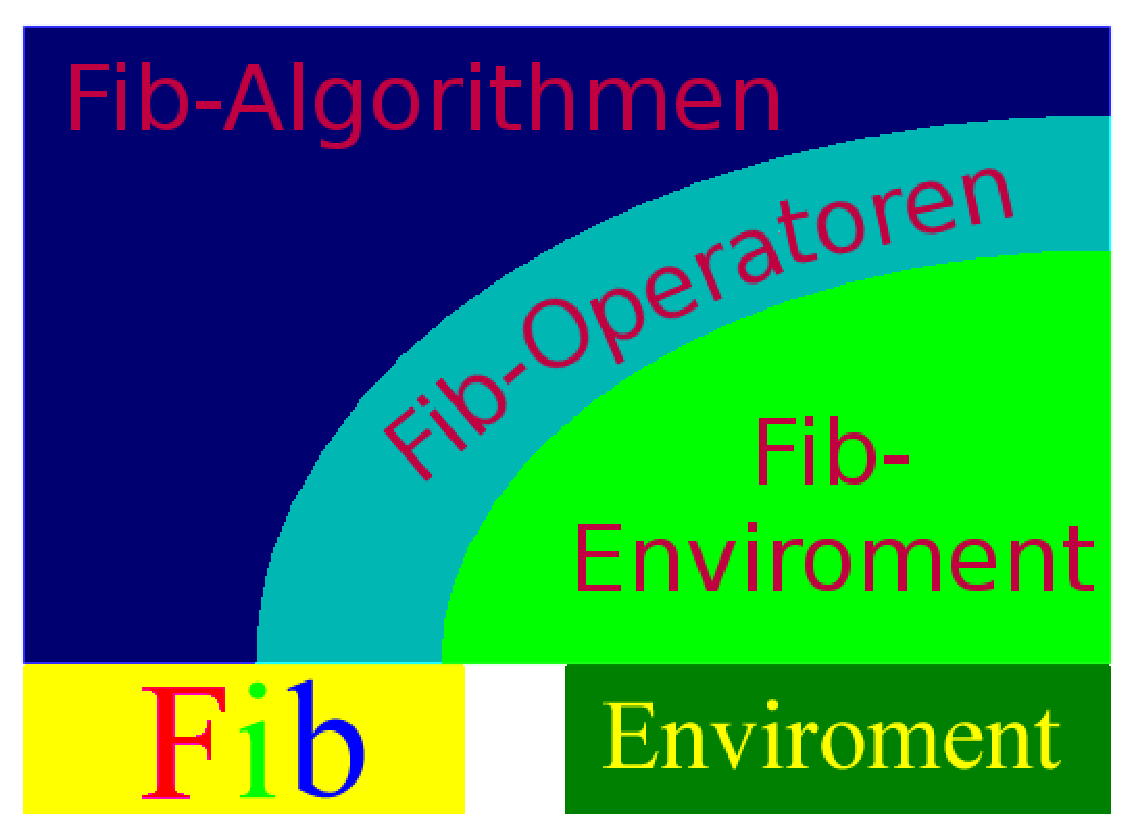
\includegraphics[scale=0.5]{ProjektAbhaengigkeiten}
\end{center}
\caption{Abh"angigkeiten der Hauptmodule}
\label{figMainModulDependencies}
\end{figure}

Das ``enviroment.fib'' Modul ben"otigt zwar f"ur seine Individuen die Fib-Objekte, dies jedoch nur als Namen (f"ur Fib-Objekte). Das ``enviroment.fib''-Modul ben"otigt also nur einen Namen f"ur Fib-Objekte und kein Wissen "uber die Funktionsweise (Methoden) der Fib-Objekte. Daher ist dass ``enviroment.fib''-Modul nicht von ``fib''-Modul abh"angig.















%TODO
%%
% Copyright (c) 2008  Betti Oesterholz
%
% Permission is granted to copy, distribute and/or modify this document
% under the terms of the GNU Free Documentation License, Version 1.2 or
% any later version published by the Free Software Foundation;
% with no Invariant Sections, no Front-Cover Texts, and no Back-Cover Texts.
%
% A copy of the license is included in the file ``fdl.tex'' .
%

%path for pictures
\graphicspath{{./klassendiagramme/}}
\graphicspath{{./klassendiagramme/}{../klassendiagramme}}


\newpage
\part{Implementation Fib-Sprachelemente}
\label{partImplementationFib}

In diesem Teil wird der Implementationsentwurf einer Bibliothek f"ur die Fib-Sprach\-ele\-mente vorgestellt. Dazu geh"ort die Klassenhierarchien und die Schnittstellenbeschreibungen. Die Schnittstellenbeschreibungen geschieht in pseudo C++.

Alle Fib-Element und Fib-Vektoren werden einem Namensraum mit dem Namen ``fib'' zugeordnet.

Alle Methoden sollten nach M"oglichkeit so definiert werden, dass es unm"oglich ist, ein ung"ultiges Fib-Objekt zu erzeugen. Das macht den Umgang mit den Methoden sicherlich schwieriger, aber auch sicherer.


\section{Hilfsmethoden}

Hilfsmethoden die bei der Implementierung Hilfreich sind, aber nicht zur eigentlichen Schnittstelle geh"oren, werden nach Bedarf implentiert, hier aber nicht aufgef"uhrt. Sie sollten nach M"oglichkeit von Au"sen nicht zugreifbar sein (also z. B. \verb|privat| oder \verb|protected| deklariert sein).


\section{Copyright}

Alle Fib-Sprachelemente werden unter die LGPL (siehe Abschnitt \ref{secLGPL} auf Seite \pageref{secLGPL}) gestellt. Auf diese Weise k"onnen sie als Bibliothek in beliebige andere Applikationen eingebunden werden.

Dies ist besonders f"ur Anzeigeprogramme/Abspielprogramme wichtig, da so die Copyright des Programms unabh"angig von der Fib-Bibliothek ist.


\section{Konstanten}

Im Fib-Namensraum werden ein paar Konstanten definiert:
\begin{itemize}
 \item \verb|FIB_VERSION|: Version der Multimediabeschreibungssprache Fib. Es handelt sich hier um eine positive ganze Zahl.
 \item \verb|FIB_DB_VERSION|: Version der Datenbank der Multimediabeschreibungssprache Fib. Es handelt sich hier um eine positive ganze Zahl.
 \item \verb|FIB_VERSION_NAME|: Name der Version der Multimediabeschreibungssprache Fib. Es handelt sich um eine Zeichenkette der Form ``Fib V1.0.2'' .
 \item \verb|FIB_DB_VERSION_NAME|: Name der Version der Datenbank der Multimediabeschreibungssprache Fib. Es handelt sich hier um eine Zeichenkette der Form ``Fib DB V2.3.1''
\end{itemize}


\section{Einfache Datentypen f"ur Zahlen}

Als primitive Datentypen f"ur Zahlen werden Fib eigene Namen benutzt, um eine einfache Erweiterbarkeit (z. B. Ausweitung des Definitionsbereichs) zu gew"ahrleisten.

\bigskip\noindent
Diese Datentypen sind:
\begin{itemize}
 \item \verb|intFib|: Ganzzahlen
 \item \verb|longFib|: nat"urliche Zahlen
 \item \verb|unsignedIntFib|: gro"se Ganzzahlen
 \item \verb|unsignedLongFib|: gro"se nat"urliche Zahlen
 \item \verb|doubleFib|: rationale Zahlen
\end{itemize}
Der Namensteil ``int'' deutet auf kleine Ganzzahlen hin und ``long'' auf gro"se. Der ``double'' Namensanfang steht f"ur Gleitkommazahlen. Beinhaltet der Name ``unsigned'' sind die Zahlen vorzeichenlos, bzw. nur positiv.

\bigskip\noindent
M"ogliche Entsprechungen in C++ k"onnten sein:
\begin{itemize}
 \item intFib: int
 \item longFib: long long
 \item doubleFib: double
 \item unsignedIntFib: unsigned int
 \item unsignedLongFib: unsigned long long
\end{itemize}


\section{Klassen f"ur Fib-Elemente}\index{Fib-Elemente}\index{Klassen!Fib-Elemente}

Sie Klasse \verb|cFibElement| ist die Basisklasse aller Fib-Elementklassen.

\bigskip\noindent
Es gibt folgende Fib-Elementklassen:
\begin{itemize}
 \item \verb|cPoint|: f"ur Punktelemente (siehe Abschnitt \ref{fibPoint} auf Seite \pageref{fibPoint})
 \item \verb|cProperty|: f"ur Eigenschaftselemente (siehe Abschnitt \ref{fibProperty} auf Seite \pageref{fibProperty})
 \item \verb|cList|: eine Liste von Fib-Objekten bzw. das Listenelement (siehe Abschnitt \ref{fibList} auf Seite \pageref{fibList})
 \item \verb|cComment|: f"ur Anmerkungselemente (siehe Abschnitt \ref{fibComment} auf Seite \pageref{fibComment})
 \item \verb|cArea|: f"ur Bereichselement (siehe Abschnitt \ref{fibArea} auf Seite \pageref{fibArea})
 \item \verb|cFunction|: f"ur Funktionselement (siehe Abschnitt \ref{fibFunction} auf Seite \pageref{fibFunction})
 \item \verb|cIf|: f"ur if-Bedingungselemente (siehe Abschnitt \ref{secFibIf} auf Seite \pageref{secFibIf})
 \item \verb|cExtObject|: f"ur externe Objekte (siehe Abschnitt \ref{fibExtObject} auf Seite \pageref{fibExtObject})
 \item \verb|cExtSubobject|: f"ur externe Unterobjekte (siehe Abschnitt \ref{fibSubobject} auf Seite \pageref{fibSubobject})
 \item \verb|cRoot|: f"ur Wurzelelemente (siehe Abschnitt \ref{fibRootElement} auf Seite \pageref{fibRootElement})
\end{itemize}
Die Fib-Elementklassen werden Klassen untergeordnet, welche ihre Struktur beschreiben:
\begin{itemize}
 \item \verb|cFibLeaf|: f"ur Fib-Elementklassen die Bl"atter sind, also keine Unterobjekte enthalten; die abgeleitete Klassen sind:
 \begin{itemize}
  \item \verb|cPoint|
  \item \verb|cExtSubobject|
 \end{itemize}
 \item \verb|cFibLimb|: f"ur Fib-Elementklassen die (gerade) Zweige sind, also genau ein Unterobjekt enthalten; die abgeleitete Klassen sind:
 \begin{itemize}
  \item \verb|cProperty|
  \item \verb|cFibList|
  \item \verb|cComment|
  \item \verb|cArea|
  \item \verb|cFunction|
 \end{itemize}
 \item \verb|cFibBranch|: f"ur Fib-Elementklassen die Verzweigungen darstellen, also mehrere Unterobjekte haben k"onnen; die abgeleitete Klassen sind:
 \begin{itemize}
  \item \verb|cFibList|
  \item \verb|cIf|
  \item \verb|cRoot|
  \item \verb|cExtObject|
 \end{itemize}
\end{itemize}

\subsection{Klassenhierarchie}\index{Fib-Elemente!Klassenhierarchie}

\begin{figure}[htbp]
\begin{center}
  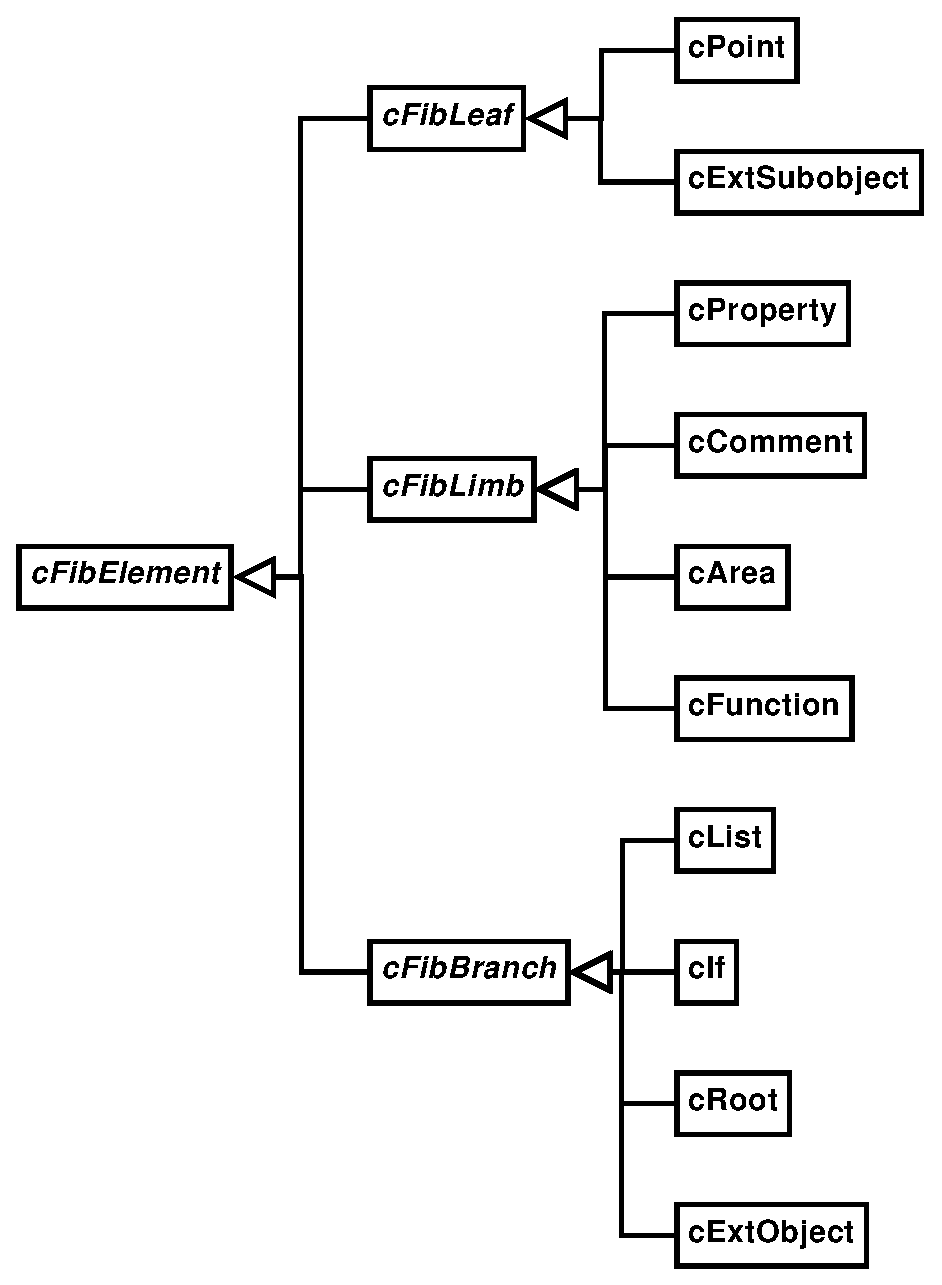
\includegraphics[scale=0.4]{fib_elemente}
\end{center}
\caption{Klassengraph Fib-Elemente}
\label{figClassFibElements}
\end{figure}

In Abbildung \ref{figClassFibElements} ist die Vererbungsstruktur der Klassen f"ur Fib-Elemente zu sehen. Wie zu sehen werden alle Fib-Elementklassen von der Klasse \verb|cFibElement| abgeleitet.


\section{Fib-Elemente Klasse cFibElement}\index{Fib-Elemente}\index{cFibElement}\index{Klassen!cFibElement}

Die Klasse \verb|cFibElement| ist die Basisklasse aller Fib-Element. Sie ist eine abstrakte Klasse, von ihr selbst k"onnen keine Objekte erzeugt werden.

\subsection{Schnittstellenbeschreibung}

Im Nachfolgenden werden die Methoden und Funktionen beschrieben, welche von allen Fib-Elementen bereitgestellt und von der Klasse \verb|cFibElement| deklariert werden. Diese Methoden und Funktionen dienen haupts"achlich dazu, die Struktur eines Fib-Objektbaums zu analysieren und anzupassen.

Externe Unterobjekte werden nur von Methoden aufgel"ost, bei denen es explizit erw"ahnt wird.

Alle Zahlen mit denen Fib-Elemente oder Objekte identifiziert werden (siehe Abschnitte "uber die Ordnung der Fib-Elemente ab Seite \pageref{secOrderFibElements}), werden bez"uglich des Fib-Elements angegeben, bei dem die entsprechende Methode aufgerufen wird, und nicht dem obersten root-Element. Soll beispielsweise das dritte Punktelement zur"uckgegeben werden, wird das dritte Punktelement bez"uglich des Fib-Elements zur"uckgegeben, an dem die entsprechende Methode aufgerufen wurde, und nicht bez"uglich des obersten root-Elements, f"ur welches dieses dritte Punktelement bez"uglich des Fib-Elements das neunte Punktelement sein k"onnte.
Dies gilt nat"urlich nur, wenn nicht explizit ein anderer Bezugspunkt angegeben wird.

\subsubsection{Typ edDirection}\index{edDirection}
\label{secEdDirection}

Der Typ \verb|edDirection| dient zur Angabe einer Richtung im Fib-Objekt. Diese Angabe sollte zu einem Referenz-Fib-Element im Fib-Objekt geschehen. (Zur Definition von ``Oben'' und ``Unten'' siehe Abschnitt \ref{secDefinitionUpDown} auf Seite \pageref{secDefinitionUpDown} .)

\bigskip\noindent
G"ultige Werte sind:
\begin{itemize}
 \item \verb|ED_ALL|: in alle Richtungen im Fib-Objekt vom Referenz-Fib-Element ausgehend
 \item \verb|ED_POSITION|: das Referenz-Fib-Element
 \item \verb|ED_BELOW|: alle Fib-Elemente unter dem Referenz-Fib-Element
 \item \verb|ED_HIGHER|: alle Fib-Elemente "uber dem Referenz-Fib-Element
 \item \verb|ED_BELOW_EQUAL|: alle Fib-Elemente unter dem Referenz-Fib-Element und das Referenz-Fib-Element
 \item \verb|ED_HIGHER_EQUAL|: alle Fib-Elemente "uber dem Referenz-Fib-Element und das Referenz-Fib-Element
\end{itemize}


\subsubsection{getType}\index{cFibElement!getType()}\index{getType()}
\label{secGetType}

\textbf{Syntax:} \verb|char getType() const|

\bigskip\noindent
"Uber die Methode kann der Typ des Objekts bzw. des Fib-Elements ermittelt werden.

\bigskip\noindent
\textbf{M"ogliche Typen sind:}
\begin{itemize}
 \item['u':] (=117) unbekannten Type; als Parameter einer Methode steht dieser Wert f"ur Fib-Elemente aller Typen
 \item['p':] (=112) f"ur Punkt-Elemente (cPoint)
 \item['y':] (=121) f"ur Eigenschaftselemente (cProperty)
 \item['l':] (=108) f"ur Listenelemente (cListen)
 \item['c':] (=110) f"ur Anmerkungselemente (cComment)
 \item['a':] (=97) f"ur Bereichselemente (cArea)
 \item['f':] (=102) f"ur Funktionselemente (cFunction)
 \item['i':] (=105) f"ur if-Bedingungen (cIf)
 \item['o':] (=111) f"ur externe Objekte (cExtObject)
 \item['s':] (=115) f"ur externe Unterobjekte (cExtSubobject)
 \item['v':] (=118) f"ur set-Elemente (cFibSet)
 \item['m':] (=109) f"ur Matrixelement (cFibMatrix)
 \item['r':] (=114) f"ur Wurzelelemente (cRoot)
\end{itemize}

\noindent
\textbf{Eingabeparameter:} keine

\bigskip\noindent
\textbf{R"uckgabe:} Es wird eine Konstante zum Identifizieren des Objekts zur"uckgegeben.


\subsubsection{getTypeName}\index{cFibElement!getTypeName()}\index{getTypeName()}

\textbf{Syntax:} \verb|static string getTypeName( char cType ) const|

\bigskip\noindent
Diese Methode wandelt das Typezeichen eines Fib-Elements in dessen Bezeichnung um.

\bigskip\noindent
\textbf{Eingabeparameter:}
\begin{itemize}
 \item \verb|cType:| Das Typzeichen, welches umzuwandeln ist.
\end{itemize}
\textbf{R"uckgabe:} Der Text f"ur die Elementbezeichnung f"ur den eingegeben Typen:

\begin{center}
\begin{tabular}{|p{20mm}|p{30mm}|}\hline
	Typ\-zeichen & Elementbezeichnung \\\hline\hline
	'u' & ``unknown''\\\hline
	'p' & ``point''\\\hline
	'y' & ``property''\\\hline
	'l' & ``list''\\\hline
	'm' & ``comment''\\\hline
	'a' & ``area''\\\hline
	'f' & ``function''\\\hline
	'i' & ``if''\\\hline
	'o' & ``extern object''\\\hline
	's' & ``extern subobject''\\\hline
	'r' & ``root''\\\hline
\end{tabular}
\end{center}

\subsubsection{getSuperiorFibElement}\index{cFibElement!getSuperiorFibElement()}\index{getSuperiorFibElement()}

\textbf{Syntax:} \verb|cFibElement* getSuperiorFibElement()|

\bigskip\noindent
Die Methode holt das n"achste Fib-Element im Fib-Baum, welches dieses Fib-Element enth"alt. Wenn kein solches Fib-Element existiert, wird ein Nullpointer \verb|NULL| zur"uckgegeben.

\bigskip\noindent
\textbf{Eingabeparameter:} keine

\bigskip\noindent
\textbf{R"uckgabe:} Einen Zeiger auf das n"achste Fib-Element, welches dieses Fib-Element enth"alt, oder der Nullpointer \verb|NULL|, wenn kein solches Fib-Element existiert.


\subsubsection{getNextFibElement}\index{cFibElement!getNextFibElement()}\index{getNextFibElement()}
\textbf{Syntax:} \verb|cFibElement* getNextFibElement()|

\bigskip\noindent
Die Methode holt das n"achste Fib-Element im Fib-Baum. Wenn kein solches Fib-Element existiert, wird ein Nullpointer \verb|NULL| zur"uckgegeben. Die Reihenfolge bezieht sich auf die Ordnung der Fib-Elemente.

\bigskip\noindent
\textbf{Eingabeparameter:} keine

\bigskip\noindent
\textbf{R"uckgabe:} Einen Zeiger auf das n"achste Fib-Element oder der Nullpointer \verb|NULL|, wenn kein solches Fib-Element existiert.


\subsubsection{getNextFibElement}\index{cFibElement!getNextFibElement()}\index{getNextFibElement()}

\textbf{Syntax:} \verb|cFibElement* getNextFibElement( char cType )|

\bigskip\noindent
Die Methode holt das n"achste Fib-Element im Fib-Baum vom angegeben Typ. Wenn kein solches Fib-Element existiert, wird ein Nullpointer \verb|NULL| zur"uckgegeben. Die Reihenfolge bezieht sich auf die Ordnung der Fib-Elemente.

\bigskip\noindent
\textbf{Eingabeparameter:}
\begin{itemize}
 \item \verb|cType|: Der Typ des Fib-Elements, welches zur"uckgegeben werden soll. Der Typ 'w' steht f"ur das n"achste Falsche (=``wrong'') Fib-Element, also ein Fib-Element, welches noch nicht korrekt mit Parametern beladen ist (es fehlt beispielsweise ein Unterobjekt).
\end{itemize}

\bigskip\noindent
\textbf{R"uckgabe:} Einen Zeiger auf das n"achste Fib-Element mit dem angegeben Typ oder der Nullpointer \verb|NULL|, wenn kein solches Fib-Element existiert.


\subsubsection{getFibElement}\index{cFibElement!getFibElement()}\index{getFibElement()}

\textbf{Syntax:} \verb|cFibElement* getFibElement( longFib lNumber,| \\\verb| bool bAbsolute=false )|

\bigskip\noindent
Die Methode holt das \verb|lNumber|'te Fib-Element. Wenn kein solches Fib-Element existiert, wird ein Nullpointer \verb|NULL| zur"uckgegeben.

\bigskip\noindent
\textbf{Eingabeparameter:}
\begin{itemize}
 \item \verb|lNumber|: Die Nummer, die das zu holende Fib-Element im aktuellen Fib-Baum/Objekt hat.
 \item \verb|bAbsolute|: Wenn \verb|bAbsolute| gleich \verb|true| ist, bezieht sich die \verb|lNumber| auf das gesamte Fib-Objekt. Ansonsten, wenn \verb|bAbsolute| gleich \verb|false| ist, bezieht sich \verb|lNumber| auf das Fib-Element von dem aus die Methode aufgerufen wurde. Standardwert ist \verb|false|.
\end{itemize}

\bigskip\noindent
\textbf{R"uckgabe:} Einen Zeiger auf das Fib-Element, vom Typ des aktuellen Fib-Elements, welches an der angegebene Position \verb|lNumber| steht oder der Nullpointer \verb|NULL|, wenn kein solches Fib-Element existiert.


\subsubsection{getFibElement}\index{cFibElement!getFibElement()}\index{getFibElement()}

\textbf{Syntax:} \verb|cFibElement* getFibElement(| \\\verb| char cType, longFib lNumber,| \\\verb| bool bAbsolute=false )|

\bigskip\noindent
Die Methode holt das \verb|lNumber|'te Fib-Element von dem angegebenen Typ \verb|cType|. Wenn kein solches Fib-Element existiert, wird ein Nullpointer \verb|NULL| zur"uckgegeben.

\bigskip\noindent
\textbf{Eingabeparameter:}
\begin{itemize}
 \item \verb|cType|: Der Typ des Fib-Elements, welches zur"uck geliefert werden soll. Der Typ 'w' steht f"ur das n"achste Falsche (=``wrong'') Fib-Element, also ein Fib-Element, welches noch nicht korrekt mit Parametern beladen ist (es fehlt beispielsweise ein Unterobjekt).
 \item \verb|lNumber|: Die Nummer, die das zu holende Fib-Element im aktuellen Fib-Baum/Objekt hat.
 \item \verb|bAbsolute|: Wenn \verb|bAbsolute| gleich \verb|true| ist, bezieht sich die \verb|lNumber| auf das gesamte Fib-Objekt. Ansonsten, wenn \verb|bAbsolute| gleich \verb|false| ist, bezieht sich \verb|lNumber| auf das Fib-Element von dem aus die Methode aufgerufen wurde. Standardwert ist \verb|false|.
\end{itemize}

\bigskip\noindent
\textbf{R"uckgabe:} Einen Zeiger auf das Fib-Element, vom angegeben Typ \verb|cType|, welches an der angegebene Position \verb|lNumber| steht oder der Nullpointer \verb|NULL|, wenn kein solches Fib-Element existiert.


\subsubsection{getAllFibElements}\index{cFibElement!getAllFibElements()}\index{getAllFibElements()}

\textbf{Syntax:} \verb|list<cFibElement*> getAllFibElements(| \\\verb| char cTypeBasis='u',| \\\verb| longFib lNumber=0, char cType='u',| \\\verb| edDirection direction=ED_ALL , unsignedLongFib| \\\verb| lNumberOfMaxReturnedElements=0 | \\\verb| bool bAbsolute=false )|

\bigskip\noindent
Die Methode gibt eine Liste mit den Zeigern zu den Fib-Elemente vom angegebenen Typ \verb|cType| zur"uck, welche sich in der Richtung \verb|direction| (siehe \ref{secEdDirection} Seite \pageref{secEdDirection}) vom \verb|lNumber|'te Objekt vom angegeben Typ \verb|cTypBasis| befinden.

Dabei werden  niemals mehr als \verb|lNumberOfMaxReturnedElements| Fib-Element zur"uckgegeben, wobei der Wert $0$ bei \verb|lNumberOfMaxReturnedElements| f"ur unendlich steht. Alle zur"uckgegebenen Fib-Elemente stammen aus dem Ast, in dem sich auch das Referenz-Fib-Element befindet.

Wenn von mehreren Richtungen oder/und Unterobjekten Fib-Elemente zur"uckzugeben sind, wird versucht von jeder Richtung oder/und Unterobjekt die gleiche Anzahl Fib-Elemente zur"uckzugeben.

\bigskip\noindent
\textbf{Eingabeparameter:}
\begin{itemize}
 \item \verb|cTypeBasis|: Der Typ, welchen das Referenz-Fib-Element im aktuellen Fib-Baum/Objekt hat. Standardwert ist 'u', womit Fib-Elemente aller Typen (bzw. keines bestimmten Typs) betrachtet werden.
 \item \verb|lNumber|: Die Nummer, welches das Referenz-Fib-Element im aktuellen Fib-Baum/Objekt hat. Standardwert ist $0$, womit alle Fib-Elemente vom aktuellen Fib-Element ausgehend zur"uckgeliefert werden, unabh"angig vom angegeben Typ \verb|cTypeBasis|.
 \item \verb|cType|: Der Typ der Fib-Elemente, welche zur"uck geliefert werden soll. Standardwert ist 'u', womit Fib-Elemente aller Typen (bzw. keines bestimmten Typs) zur"uckgegeben werden. Der Typ 'w' steht f"ur Falsche (=``wrong'') Fib-Elemente, also Fib-Elemente, welche noch nicht korrekt mit Parametern beladen sind (es fehlt beispielsweise ein Unterobjekt).
 \item \verb|direction|: Die Richtung vom Referenz-Fib-Element ausgehend, von der alle Fib-Elemente mit dem angegeben Typ zur"uckzugeben sind. Standardwert ist hierf"ur \verb|ED_ALL|, so dass Fib-Elemente aus dem gesamten Ast des Referenz-Fib-Elements zur"uckgegeben werden.
 \item \verb|lNumberOfMaxReturnedElements|: Die Anzahl der maximal zur"uckzugebenden Fib-Elemente. Ist der Wert $0$, gibt es keine Begrenzung f"ur die Anzahl der zur"uckzugebenden Fib-Elemente. Standardwert ist $0$ (=unbegrenzt).
 \item \verb|bAbsolute|: Wenn \verb|bAbsolute| gleich \verb|true| ist, bezieht sich die \verb|lNumber| auf das gesamte Fib-Objekt. Ansonsten, wenn \verb|bAbsolute| gleich \verb|false| ist, bezieht sich \verb|lNumber| auf das Fib-Element von dem aus die Methode aufgerufen wurde. Standardwert ist \verb|false|.
\end{itemize}

\bigskip\noindent
\textbf{R"uckgabe:} Eine Liste mit den entsprechenden Fib-Elementen.


\subsubsection{evalueObject}\index{cFibElement!evalueObject()}\index{evalueObject()}
\label{secEvalueObjectPosition}

\textbf{Syntax:} \verb|bool evalueObject(| \\\verb| iEvaluePosition & evaluePosition,| \\\verb| const unsignedIntFib objectPoint=0,| \\\verb| list<cVectorProperty> &liVecProperties=| \\\verb| list<cVectorProperty>() ) const|

\bigskip\noindent
"Uber die Methode \verb|evalueObject| k"onnen Fib-Objekte ausgewertet werden.

Der Methode wird eine Referenz auf ein Object (\verb|evaluePosition|) vom Type \verb|iEvaluePosition| "ubergeben, "uber welche die einzelnen Punkt mit ihren Eigenschaften ausgewertet werden. Jedes mal, wenn ein Punkt dargestellt/ ausgewertet werden soll, wird die Methode \verb|evaluePosition()| des Objects mit der Position des Punktes und einer Liste seiner Eigenschaften aufgerufen. Auf diese Weise kann die Methode \verb|evalueObject| f"ur verschiedene Aufgaben genutzt werden. Soll ein Objekt als Bild ausgewertet werden, stellt die Methode \verb|evaluePosition()| einen Punkt im Bild dar. Wenn das Objekt mit einem anderen Multimediaobjekt verglichen werden soll, vergleicht die Methode \verb|evaluePosition()| die einzelnen Punkte (Vorsicht ist geboten, wenn ein Punkt einen anderen "uberdeckt). Die Methode \verb|evaluePosition()| muss nur entsprechend implementiert werden.
Gibt ein Aufruf der Methode \verb|evaluePosition()| false zur"uck, wird die Auswertung des Fib-Objekts mit \verb|evalueObject| abgebrochen.
N"aheres zu Objekten, welche das Interface \verb|iEvaluePosition| implementieren im Abschnitt \ref{secIEvaluePosition} auf Seite \pageref{secIEvaluePosition} .

Von der Methode \verb|evalueObject| werden auch externe Objekte aufgel"ost. Auf diese Weise wird das komplette Multimediaobjekt ausgewertet, welches des Fib-Objekt darstellt.

\bigskip\noindent
\textbf{Eingabeparameter:} 
\begin{itemize}
 \item \verb|evaluePosition|: Eine Referenz auf ein Object zum auswerten/ speichern der einzelnen Punkte mit ihren Eigenschaften. Dieses Object stellt die Methode \verb|evaluePosition()| bereit, der f"ur jeden Punkt, der ausgewertet werden soll, die Position und eine Liste mit Eigenschaften des Punktes "ubergeben wird.
 \item \verb|objectPoint|: Der Objektpunkt des echten Teilobjekts, welches ausgewertet werden soll. Standardm"a"sig wird dieser Wert auf $0$ gesetzt und damit das gesamt Objekt ausgewertet.
 \item \verb|liVecProperties|: Eine Liste mit den Eigenschaften, die das auszuwertende Objekt global besitzen soll. Diese Eigenschaften werden jeden Punkt zugeordnet, soweit sie nicht "uberschrieben werden. Standardm"a"sig wird hier eine leere Liste, also keine globalen Eigenschaften, "ubergeben.
\end{itemize}

\bigskip\noindent
\textbf{R"uckgabe:} Diese Methode gibt \verb|true| (=wahr) zur"uck, wenn die Auswertung des Objekts erfolgreich war, sonst \verb|false| (=falsch).


\subsubsection{evalueObject}\index{cFibElement!evalueObject()}\index{evalueObject()}
\label{secEvalueObjectFibElement}

\textbf{Syntax:} \verb|bool evalueObject(| \\\verb| iEvalueFibElement & evalueFibElement,| \\\verb| const unsignedIntFib objectPoint=0,| \\\verb| list<cVectorProperty> &liVecProperties=| \\\verb| list<cVectorProperty>(),| \\\verb| conat list<char> liCFibElementTyps )|


\bigskip\noindent
"Uber die Methode \verb|evalueObject| k"onnen Fib-Objekte ausgewertet werden.

Der Methode wird eine Referenz auf ein Object (\verb|evalueFibElement|) vom Type \verb|iEvalueFibElement| "ubergeben, "uber welche die einzelnen Fib-Elemente mit ihren Eigenschaften ausgewertet werden. Jedes mal, wenn ein Fib-Elemente dargestellt/ ausgewertet werden soll, wird die Methode \verb|evalueElement()| des Objects mit einem Zeiger auf des Fib-Elemente und einer Liste seinen Eigenschaften aufgerufen. Auf diese Weise kann die Methode \verb|evalueObject| f"ur verschiedene Aufgaben genutzt werden.
Gibt ein Aufruf der Methode \verb|evalueElement()| false zur"uck, wird die Auswertung des Fib-Objekts mit \verb|evalueObject| abgebrochen.
N"aheres zu Objekten, welche das Interface \verb|iEvalueFibElement| implementieren im Abschnitt \ref{secIEvalueFibElement} auf Seite \pageref{secIEvalueFibElement} .

"Uber die Liste \verb|liCFibElementTyps| wird bestimmt, welche Fib-Element zur"uckgegeben werden sollen. F"ur jedes Fib-Element das zur"uckgegeben werden soll, steht in \verb|liCFibElementTyps| sein Typzeichen (siehe Abschnitt \ref{secGetType} auf Seite \pageref{secGetType}). Punktelemente mit Positionsvektoren werden immer zur"uckgegeben. Diese m"u"sen nicht seperat in \verb|liCFibElementTyps| aufgef"uhrt werden.

\bigskip\noindent
\textbf{Eingabeparameter:} 
\begin{itemize}
 \item \verb|evalueFibElement|: Eine Referenz auf ein Object zum auswerten/ speichern der einzelnen Fib-Elemente mit ihren Eigenschaften. Dieses Object stellt die Methode \verb|evalueElement()| bereit, der f"ur jedes Fib-Element, mit einem Type aus der Liste \verb|liCFibElementTyps| oder das ein Punkt ist, ein Zeiger auf das Fib-Element und eine Liste mit Eigenschaften des Fib-Elements "ubergeben wird.
 \item \verb|objectPoint|: Der Objektpunkt des echten Teilobjekts, welches ausgewertet werden soll. Standardm"a"sig wird dieser Wert auf $0$ gesetzt und damit das gesamt Objekt ausgewertet.
 \item \verb|liVecProperties|: Eine Liste mit den Eigenschaften, die das auszuwertende Objekt global besitzen soll. Diese Eigenschaften werden jeden Blattelement zugeordnet, soweit sie nicht "uberschrieben werden. Standardm"a"sig wird hier eine leere Liste, also keine globalen Eigenschaften, "ubergeben.
 \item \verb|liCFibElementTyps|: Die Liste mit den Typzeichen f"ur die Fib-Element, f"ur die \verb|auf()| aufgerufen werden soll. Die m"oglichen Zeichen werden in Abschnitt \ref{secGetType} auf Seite \pageref{secGetType} aufgef"uhrt.
\end{itemize}

\bigskip\noindent
\textbf{R"uckgabe:} Diese Methode gibt \verb|true| (=wahr) zur"uck, wenn die Auswertung des Objekts erfolgreich war, sonst \verb|false| (=falsch).


\subsubsection{getTimeNeed}\index{cFibElement!getTimeNeed()}\index{getTimeNeed()}\index{Auswertungszeit}

\textbf{Syntax:} \verb|unsignedLongFib getTimeNeed( | \\\verb| unsignedLongFib lMaxTime=0 ) const|

\bigskip\noindent
Diese Methode berechnet einen Wert f"ur die Zeit, welche zur Auswertung des Fib-Objekts ben"otigt wird.

Von der Methode \verb|getTimeNeed| werden auch externe Objekte aufgel"ost und in der Berechnung ber"ucksichtigt.

Der Eingabeparameter \verb|lMaxTime| dient dazu, den Aufwand zum Berechnen der Zeit zu begrenzen. Wenn ein Fib-Objekt sehr Zeitaufw"andig auszuwerten ist, w"urde auch das Ermitteln der Zeitstatistik entsprechend lange dauern. Mit dem Parameter \verb|lMaxTime| wird die Zeit zur Berechnung der Zeitstatistik begrenzt bzw. abgebrochen, wenn \verb|lMaxTime| erreicht wurde. Wenn der Wert \verb|lMaxTime| nicht angegeben wird oder $0$ ist, wird die Berechnungszeit nicht begrenzt.

N"utzlich ist diese Begrenzung, da eine genetische Operation die Auswertungszeit sehr stark erh"ohen kann. Durch die Begrenzung kann die Zeit zum Ermitteln der Zeitstatistik begrenzt werden und alle Individuen, die diese Grenze erreichen sofort verworfen/ gel"oscht werden.

In Tabelle \ref{tabTimeNeed} sind die Formeln f"ur die ben"otigten Zeiten f"ur die einzellnen Elemente aufgef"uhrt. Dabei bezeichnet $T$ die Auswertungszeit eines Fib-Elements und $T(Obj_i)$ die Auswertungszeit des i'ten enthaltenden Fib-Objekts.

\begin{center}
\begin{longtable}{|p{22mm}|p{50mm}|p{50mm}|}\hline
	Fib-Ele\-ment\-klasse & Zeitformel & Anmerkung \\\hline\endhead

	\verb|cPoint|    & $T(Obj)= 1 + E_V$ & $E_V$ ist die Anzahl der Elemente des Positionsvektors \\\hline
	\verb|cProperty| & $T(Obj)= 1 + E_V + T(Obj_1)$ & $E_V$ ist die Anzahl der Elemente des Eigenschaftsvektor; $T(Obj_1)$ die Auswertungszeit des enthaltenden Fib-Objekts $Obj_1$\\\hline
	\verb|cFibList|  & $T(Obj)= 1 + \sum^{n}_{i=1} T(Obj_i)$ & $T(Obj_i)$ sind die Auswertungszeiten der enthaltenden Fib-Unterobjekte $Obj_i$; $n$ ist die Anzahl der enthaltenden Fib-Unterobjekte\\\hline
	\verb|cComment|: & $T(Obj)= 1 + T(Obj_1)$ & $T(Obj_1)$ ist die Auswertungszeit des enthaltenden Fib-Objekts $Obj_1$\\\hline
	\verb|cArea|: & $T(Obj)= 1 + \sum_{W \in B_1 \ldots B_n} T( Obj_1(W) )$ & $B_i$ sind die Unterbereiche des Bereichs, mit $n$ der Anzahl der Unterbereiche; $W$ sind dann die einzelnen Werte der Bereiche; $T( Obj_1(W) )$ ist die Auswertungszeit des enthaltenden Fib-Objekts $Obj_1$, wenn die Variable des Bereichselements auf $W$ gesetzt wurde \\\hline
	\verb|cFunction| & $T(Obj)= T(UF) + T( Obj_1(W) )$ & $T(UF)$ ist die Zeit, welche zu Berechnen der Unterfunktion ben"otigt wird;  $T( Obj_1(W) )$ ist die Auswertungszeit des enthaltenden Fib-Objekts $Obj_1$, wenn die Variable des Funktionselements auf $W$, den Wert der Funktion, gesetzt wurde \\\hline
	\verb|cIf|       & $T(Obj)= T(UB) + if ( UB==true )\{ T(Obj_1)\} else \{ T(Obj_2)\}$ & $T(UB)$ ist die Zeit, welche zu Berechnen der Unterbedingung ben"otigt wird; $T(Obj_1)$ und $T(Obj_2)$ die Auswertungszeiten der enthaltenden Fib-Objekte $Obj_1$ und $Obj_2$, es wird jeweils die Auswertungszeit desjenigen Objekts hinzuaddiert, welches bei der Unterbedingungsauswertung auch ausgewertet w"urde (als $Obj_1$ wenn die Unterbedingung wahr ist und sonst $Obj_2$)\\\hline
	\verb|cExtObject| & $T(Obj)= 5 + T(Obj_1)$ & $T(Obj_1)$ ist die Auswertungszeit des Fib-Objekts $Obj_1$, welches durch das externe Objekte repr"asentiert wird\\\hline
	\verb|cExtSub-| \verb|object| & $T(Obj)= 2 + T(Obj_1)$ & $T(Obj_1)$ ist die Auswertungszeit des Fib-Objekts $Obj_1$, welches hier jeweils eingesetzt bzw. extern bereitgestellt wird\\\hline
	\verb|cFibSet| & $T(Obj)= n * \sharp DefVar +$ $\sum_{V \in V_1 \ldots V_n} T( Obj_1(V) )$ & $\sharp DefVar$ ist die Anzahl der vom set-Element definierten Variablen;$V_i$ sind die Vektoren mit den zu setzenden Werten des set-Elements, mit $n$ der Anzahl der Vektoren; $V$ sind dann die einzelnen Vektoren; $T( Obj_1(V) )$ ist die Auswertungszeit des enthaltenden Fib-Objekts $Obj_1$, wenn die definierten Variable des set-Elements auf die entsprechenden Elementwerte von $V$ gesetzt wurden \\\hline
	\verb|cFibMatrix| & $T(Obj)= if ( i not 0 )\{$ $\sum_{V \in V_1 \ldots V_k}( d + i + T( Obj_1(D(V),V) ) )$ $\}else\{$ $\sum_{v_1 = Startvalue_1 \ldots Endvalue_1} \ldots$ $sum_{v_d = Startvalue_d \ldots Endvalue_d} ($ $d + T( Obj_1(v_1, \ldots, v_d ) ) ) \}$ &  Die Zeitbereichnung von Matrixelementen ist davon Abh"angig, ob Variablen f"ur die Werte vorhanden sind ($0 < i$). Sind Variablen f"ur die Werte vorhanden ($0 < i$), wird f"ur jeden Wertevektor $V=(W_{1.b}, \ldots, W_{n.b})$ das enthaltende Objekt $Obj_1$ mit aufgerufen / ausgewertet bzw. die Zeit f"ur diesen Aufruf addiert. Dabei werden die Wertevariablen mit den entsprechenden Werten belegt und die Dimensionsvariablen mit den entsprechend hochgez"ahlten Werten $D(V)$ (in $Obj_1(D(V),V)$). Zu der Zeit des Aurufs des enthaltende Objekts $Obj_1$ wird noch die Zeit zur Belegung der Variablen addiert ($d + i$).    Wenn keine Variablen f"ur die Werte vorhanden sind ($i==0$), durchlaufen die Dimensionsvariablen jeweils ihre Bereiche, wobei f"ur jede Belegung das enthaltende Objekt ausgewertet wird. Die Zeit ist also f"ur jede Dimensionsvariablenbelegung die Zeit f"ur die Belegung dieser $d$ plus die Auswertungzeit des enthaltende Objekts f"ur diese Belegung. \\\hline

	\verb|cRoot|      & $T(Obj)= 3 + T(Obj_1)$ & $T(Obj_1)$ ist die Auswertungszeit des enthaltenden Haupt-Fib-Objekts $Obj_1$\\\hline

	nullstellige Unterfunktionen & $T(UF)= 1$ & F"ur jede Unterfunktionen oder Unterbedingungen wird jeweils $1$ hinzuaddiert \\\hline
	einstellige Unterfunktionen & $T(UF)= 1 + T( UF_1 )$ & $UF_1$ ist die enthaltende Unterfunktion \\\hline
	zweistellige Unterfunktionen & $T(UF)= 1 + T( UF_1 ) + T( UF_2 )$ & $UF_1$ und $UF_2$ sind die enthaltenden Unterfunktionen \\\hline

	nullstellige Unterbedingungen & $T(UB)= 1$ & F"ur jede Unterfunktionen oder Unterbedingungen wird jeweils $1$ hinzuaddiert \\\hline
	einstellige Unterbedingungen & $T(UB)= 1 + T( UB_1 )$ & $UB_1$ ist die enthaltende Unterbedingung \\\hline
	zweistellige Unterbedingungen & $T(UB)= 1 + T( UB_1 ) + T( UB_2 )$ & $UB_1$ und $UB_2$ sind die enthaltenden Unterbedingungen \\\hline
	Vergleiche & $T(UB)= 1  + T( UF_1 ) + T( UF_2 )$ & $UF_1$ und $UF_2$ sind die enthaltenden Unterfunktionen \\\hline

%TODO Unterfunktionen + Unterbedingungen detailiert
\caption{Auswertungszeiten $T(Obj)$ der Fib-Objekts $Obj$}
\label{tabTimeNeed}
\end{longtable}
\end{center}


\bigskip\noindent
\textbf{Eingabeparameter:} 
\begin{itemize}
 \item \verb|lMaxTime|: Der Wert \verb|lMaxTime| der bei der Zeitberechnung nicht "uberschritten werden soll. Ist \verb|lMaxTime=0| (Standardwert), wird die Zeitberechnung nicht begrenzt.
\end{itemize}

\bigskip\noindent
\textbf{R"uckgabe:} Diese Methode berechnet einen Wert f"ur die Zeit, welche zur Auswertung des Fib-Objekts ben"otigt wird.


\subsubsection{getCompressedSize}\index{cFibElement!getCompressedSize()}\index{getCompressedSize()}

\textbf{Syntax:} \verb|unsignedLongFib getCompressedSize() const|

\bigskip\noindent
Diese Methode gibt die Anzahl der Bits f"ur die Gr"o"se des Fib-Objekts zur"uck. Dabei wird f"ur jedes Element (Fib-Element, Fib-Vektoren, usw.) ein Wert aufaddiert, der den Speicherplatzbedarf in Bit beim komprimierten Abspeichern des Elements entspricht (siehe Abschnitt \ref{fibCompressing} auf Seite  \pageref{fibCompressing}).

Bei der Berechnung der Gr"o"se werden keine externen Objekte aufgel"ost, sondern nur die Struktur des aktuellen Fib-Objekts ausgewertet.
Weiterhin werden die optionale Information ($Optionalpart$) der root-Elemente nicht mit eingerechnet, da sie als optionale Informationen weggelassen werden k"onnen.

\bigskip\noindent
\textbf{Eingabeparameter:} keine

\bigskip\noindent
\textbf{R"uckgabe:} Diese Methode liefert einen Wert f"ur die Gr"o"se in Bits des Fib-Objekts zur"uck.


\subsubsection{isUsedVariable}\index{cFibElement!isUsedVariable()}\index{isUsedVariable()}

\textbf{Syntax:} \verb|bool isUsedVariable( const cFibVariable *variable,| \\\verb| edDirection direction=ED_POSITION ) const|

\bigskip\noindent
Diese Methode pr"uft, ob die gegebene Variable \verb|variable| in den Fib-Elementen, in der angegeben Richtung \verb|direction| vom Fib-Element (von dem die Methode aufgerufen wird) ausgehend, benutzt wird (z. B. in einem Vektor vorkommt).

Diese Methode kann beispielsweise dazu verwendet werden, um zu Pr"ufen, ob ein Fib-Element, das eine Variable definiert, gel"oscht werden kann.

\bigskip\noindent
\textbf{Eingabeparameter:} 
\begin{itemize}
 \item \verb|variable|: Die Variable f"ur die gepr"uft werden soll, ob sie benutzt wird.
 \item \verb|direction|: Die Richtung, vom aktuellem Fib-Element ausgehend, in der sich die zu pr"ufenden Fib-Elemente befinden. Standardm"a"sig wird nur das aktuelle Fib-Element gepr"uft.
\end{itemize}

\bigskip\noindent
\textbf{R"uckgabe:} Die Methode gibt \verb|true| (=wahr) zur"uck, wenn die Variable in den Fib-Elementen benutzt wird, sonst \verb|false| (=falsch).


\subsubsection{getUsedVariables}\index{cFibElement!getUsedVariables()}\index{getUsedVariables()}

\textbf{Syntax:} \verb|set<cFibVariable*> getUsedVariables(| \\\verb| edDirection direction=ED_POSITION )|

\bigskip\noindent
Diese Methode gibt die Menge aller Variablen zur"uck, die in den Fib-Elementen in der angegeben Richtung \verb|direction| vom Fib-Element, von dem die Methode aufgerufen wird, ausgehend, benutzt werden (bzw. in einem Vektor vorkommt).

\bigskip\noindent
\textbf{Eingabeparameter:} 
\begin{itemize}
 \item \verb|direction|: Die Richtung, vom aktuellem Fib-Element ausgehend, in der sich die Fib-Elemente befinden, von denen die benutzten Variablen zur"uckgegeben werden sollen. Standardm"a"sig wird nur das aktuelle Fib-Element gepr"uft.
\end{itemize}

\bigskip\noindent
\textbf{R"uckgabe:} Diese Methode gibt die Menge aller Variablen zur"uck, die in den Fib-Elementen in der angegeben Richtung \verb|direction| vom Fib-Element, von dem die Methode aufgerufen wird, ausgehend, benutzt werden (bzw. in einem Vektor vorkommt).


\subsubsection{isDefinedVariable}\index{cFibElement!isDefinedVariable()}\index{isDefinedVariable()}

\textbf{Syntax:} \verb|bool isDefinedVariable(| \\\verb| const cFibVariable *variable,| \\\verb| edDirection direction=ED_POSITION) const|

\bigskip\noindent
Diese Methode pr"uft, ob die gegebene Variable \verb|variable| in einem Fib-Element definiert ist, welches in der angegeben Richtung \verb|direction| vom aktuellen Fib-Element ausgehend stehen.

Variablen werden beispielsweise von Bereichs- oder Funktionselementen definiert.

Variablen, die ein root-Element definiert, liegen nicht "uber den in diesem root-Element enthaltenden unter-root-Elemente. Daher kann keine Variable "uber einem root-Element definiert sein. Dies liegt daran, dass root-Element die Variablen, die sie definieren, nicht an enthaltende root-Elemente vererben, daher k"onnen sie auch nicht in enthaltenden root-Elementen benutzt werden.

\bigskip\noindent
\textbf{Eingabeparameter:} 
\begin{itemize}
 \item \verb|variable|: Die Variable f"ur die gepr"uft werden soll, ob sie definiert wird.
 \item \verb|direction|:Die Richtung, vom aktuellem Fib-Element ausgehend, in der sich die zu pr"ufenden Fib-Elemente befinden. Standardm"a"sig wird das aktuelle Fib-Elemente gepr"uft.
\end{itemize}

\bigskip\noindent
\textbf{R"uckgabe:} Die Methode gibt \verb|true| (=wahr) zur"uck, wenn die Variable in einem der gepr"uften Fib-Elemente definiert wird, sonst \verb|false| (=falsch).


\subsubsection{getDefinedVariables}\index{cFibElement!getDefinedVariables()}\index{getDefinedVariables()}

\textbf{Syntax:} \verb|list<cFibVariable*> getDefinedVariables(| \\\verb| edDirection direction=ED_HIGHER )|

\bigskip\noindent
Diese Methode gibt die Menge aller Variablen zur"uck, die in den Fib-Elementen in der angegeben Richtung \verb|direction| vom Fib-Element, von dem die Methode aufgerufen wird, ausgehend, definiert werden.

Variablen, die ein root-Element definiert, liegen nicht "uber den in diesem root-Element enthaltenden unter-root-Elemente. Daher kann keine Variable "uber einem root-Element definiert sein. Dies liegt daran, dass root-Element die Variablen, die sie definieren, nicht an enthaltende root-Elemente vererben, daher k"onnen sie auch nicht in enthaltenden root-Elementen benutzt werden.

\bigskip\noindent
\textbf{Eingabeparameter:} 
\begin{itemize}
 \item \verb|direction|: Die Richtung, vom aktuellem Fib-Element ausgehend, in der sich die Fib-Elemente befinden, von denen die definierten Variablen zur"uckgegeben werden sollen. Standardm"a"sig werden alle Fib-Element, die das aktuelle Fib-Element direkt oder indirekt enthalten, gepr"uft.
\end{itemize}

\bigskip\noindent
\textbf{R"uckgabe:} Diese Methode gibt eine Liste aller Variablen zur"uck, die in den Fib-Elementen in der angegeben Richtung \verb|direction| vom Fib-Element, von dem die Methode aufgerufen wird, ausgehend, definiert werden.


\subsubsection{replaceVariable}\index{cFibElement!replaceVariable()}\index{replaceVariable()}

\textbf{Syntax:} \verb|bool replaceVariable( cFibVariable *variableOld,| \\\verb| cFibVariable *variableNew )|

\bigskip\noindent
Diese Methode ersetzt im Fib-Object die Vorkommen der Variable \verb|variableOld| durch die Variable \verb|variableNew| .

Dabei bleiben Definitionen von Variablen \verb|variableOld| unber"uhrt. Es werden also nur Vorkommen ge"andert an denen die Variable \verb|variableOld| benutzt wird.

\bigskip\noindent
\textbf{Eingabeparameter:} 
\begin{itemize}
 \item \verb|variableOld|: Die Variable, die ersetzt werden soll.
 \item \verb|variableNew|: Die Variable, welche die Variable \verb|variableOld| ersetzen soll.
\end{itemize}

\bigskip\noindent
\textbf{R"uckgabe:} Die Methode gibt \verb|true| (=wahr) zur"uck, wenn die \verb|variableOld| Variable dem Fib-Object durch die Variable \verb|variableNew| ersetzt wurde, sonst \verb|false| (=falsch).


\subsubsection{getNumberOfElement}\index{cFibElement!getNumberOfElement()}\index{getNumberOfElement()}

\textbf{Syntax:} \verb|unsignedIntFib getNumberOfElement(| \\\verb| bool bOfType=false )const|

\bigskip\noindent
Diese Methode gibt die Nummer des Fib-Elements in der Ordnung der Fib-Elemente zur"uck.

\bigskip\noindent
\textbf{Eingabeparameter:}
\begin{itemize}
 \item \verb|bOfType|: Wenn \verb|bOfType| falsch (=\verb|false|) ist, wird die Nummer bez"uglich der Ordnung aller Fib-Elemente zur"uckgegeben. Ist dagegen \verb|bOfType| wahr (=\verb|true|), wird die Nummer bez"uglich der Ordnung der Fib-Elemente vom gleichem Typ wie das aktuelle Fib-Element zur"uckgegeben. Der Standardwert ist falsch (=\verb|false|),
\end{itemize}

\bigskip\noindent
\textbf{R"uckgabe:} Die Nummer des Fib-Elements in der Ordnung der Fib-Elemente.


\subsubsection{getNumberOfMovePoint}\index{cFibElement!getNumberOfMovePoint()}\index{getNumberOfMovePoint()}
\textbf{Syntax:} \verb|unsignedIntFib getNumberOfMovePoint() const|

\bigskip\noindent
Gibt die Nummer des Fib-Elements in der Ordnung der Verschiebungspunkte zur"uck.

Verschiebungspunkte, sind Stellen (Positionen von Fib-Elementen) von denen und zu denen Fib-Elemente verschoben werden k"onnen. Dies sind in der Regel alle (geraden) Astelemente \verb|cFibLimb| (siehe Abschnitt \ref{secCFibLimb} auf Seite \pageref{secCFibLimb} ). Beispielsweise sind alle Bereichsobjekte Verschiebungspunkte, Punktobjekte hingegen nicht. Zm Verschieben von Fib-Elementen siehe auch Abschnitt \ref{secMoveLimbElement} auf Seite \pageref{secMoveLimbElement} .

Es wird $0$ zur"uckgegeben, wenn das aktuelle Fib-Element kein Verschiebepunkt ist, bzw. nicht verschoben werden kann.

\bigskip\noindent
\textbf{Eingabeparameter:} keine

\bigskip\noindent
\textbf{R"uckgabe:} Die Nummer des Fib-Elements in der Ordnung der Verschiebungspunkte oder $0$, wenn das Fib-Element kein Verschiebepunkt ist.


\subsubsection{getNumberOfObjectPoint}\index{cFibElement!getNumberOfObjectPoint()}\index{getNumberOfObjectPoint()}

\textbf{Syntax:} \verb|unsignedIntFib getNumberOfObjectPoint() const|

\bigskip\noindent
Diese Methode gibt die Nummer des zusammenh"angenden Teilobjekte in der Ordnung der zusammenh"angenden Teilobjekte zur"uck. Das zusammenh"angenden Teilobjekte, auf das sich bezogen wir, ist das zusammenh"angenden Teilobjekte, welches "uber dem aktuellen Fib-Element als n"achstes "uber ein Fib-Unterobjekt definiert ist. Also das Teilobjekt, welches das aktuelle Fib-Element enth"alt, aber kein zusammenh"angendes Teilobjekt enth"alt, welches auch das aktuelle Fib-Element enth"alt.

Zur Beschreibung der Ordnung von zusammenh"angenden Teilobjekte siehe Abschnitt \ref{secOrderPartobjects} auf Seite \pageref{secOrderPartobjects} .

\bigskip\noindent
\textbf{Eingabeparameter:} keine

\bigskip\noindent
\textbf{R"uckgabe:} Die Nummer in der Ordnung der zusammenh"angenden Teilobjekte des n"achsten Teilobjekts in dem das aktuelle Fib-Element vorhanden ist.


\subsubsection{getNumberOfElements}\index{cFibElement!getNumberOfElements()}\index{getNumberOfElements()}

\textbf{Syntax:} \verb|unsignedIntFib getNumberOfElements(| \\\verb| char cType='u' )| \\\verb| const|

\bigskip\noindent
Gibt die Anzahl der Fib-Elemente vom angegebenen Typ im aktuellem Fib-Objekt zur"uck.

Standardm"a"sig wird die Anzahl aller Fib-Elemente zur"uckgegeben. Der Standardtyp zum zur"uckgeben der Anzahl aller Fib-Elemente ist 'u' f"ur ``unknown'', damit wird angezeigt, dass man sich auf keinen Typ festlegt, bzw. allw Fib-Elemente gez"ahlt werden.

\bigskip\noindent
\textbf{Eingabeparameter:}
\begin{itemize}
 \item \verb|cType|: Der Typ der Elemente, deren Anzahl zur"uckgeliefert werden soll. Der Standardwert ist 'u', damit alle Fib-Elemente gez"ahlt werden.
\end{itemize}

\bigskip\noindent
\textbf{R"uckgabe:} Die Anzahl vom Fib-Elemente vom angegebenen Typ.


\subsubsection{getNumberOfMovePoints}\index{cFibElement!getNumberOfMovePoints()}\index{getNumberOfMovePoints()}
\textbf{Syntax:} \verb|unsignedIntFib getNumberOfMovePoints() const|

\bigskip\noindent
Liefert die Anzahl der Verschiebungspunkte im aktuellem Objekt.
Verschiebungspunkte, sind Stellen (Positionen von Fib-Elementen) von denen und zu denen Fib-Elemente verschoben werden k"onnen. Dies sind in der Regel alle (geraden) Astelemente \verb|cFibLimb| (siehe Abschnitt \ref{secCFibLimb} auf Seite \pageref{secCFibLimb} ). Beispielsweise sind alle Bereichsobjekte Verschiebungspunkte, Punktobjekte hingegen nicht.

Zm Verschieben von Fib-Elementen siehe auch Abschnitt \ref{secMoveLimbElement} auf Seite \pageref{secMoveLimbElement} .

\bigskip\noindent
\textbf{Eingabeparameter:} keine


\bigskip\noindent
\textbf{R"uckgabe:} Die Anzahl der Verschiebungspunkte im aktuellem Objekt.


\subsubsection{getNumberOfObjectPoints}\index{cFibElement!getNumberOfObjectPoints()}\index{getNumberOfObjectPoints()}

\textbf{Syntax:} \verb|unsignedIntFib getNumberOfObjectPoints() const|

\bigskip\noindent
Diese Methode gibt die Anzahl der zusammenh"angenden Teilobjekte im Fib-Objekt zur"uck.

Zur Beschreibung der Ordnung von zusammenh"angenden Teilobjekte siehe Abschnitt \ref{secOrderPartobjects} auf Seite \pageref{secOrderPartobjects} .

\bigskip\noindent
\textbf{Eingabeparameter:} keine

\bigskip\noindent
\textbf{R"uckgabe:} Zur"uckgegeben wird die Anzahl der zusammenh"angenden Teilobjekte im Fib-Objekt.


\subsubsection{typeElementPointToElementPoint}\index{cFibElement!typeElementPointToElementPoint()}\index{typeElementPointToElementPoint()}
%Elementpunkt von Element vom Typ x -> Elementpunkt 'u'
\textbf{Syntax:} \verb|unsignedIntFib typeElementPointToElementPoint( | \\\verb| const char cType, const unsignedIntFib elementPoint, | \\\verb| bool bAbsolute=false ) const|

\bigskip\noindent
F"ur das \verb|elementPoint|'te Element vom angegebenen Typ (\verb|cType|) im Fib-Objekt, wird die Nummer zur"uckgegeben, welche es unter allen Fib-Elementen im Fib-Objekt hat.

Damit kann beispielsweise ermittelt werden, das wievielte Fib-Element das dritte Listenelement im Fib-Objekt ist.

\bigskip\noindent
\textbf{Eingabeparameter:}
\begin{itemize}
 \item \verb|cType|: Der Typ des Fib-Elements, bez"uglich welchem die angegebene Nummer \verb|elementPoint| gilt.
 \item \verb|elementPoint|: Die Nummer des Fib-Elements unter den Fib-Elemente vom angegeben Typ \verb|cType|.
 \item \verb|bAbsolute|: Wenn \verb|bAbsolute| gleich \verb|true| (=wahr) ist, beziehen sich die Ordnungen auf das gesamte Fib-Objekt. Ansonsten, wenn \verb|bAbsolute| gleich \verb|false| (=falsch) ist, beziehen sich Ordnungen auf das Fib-Element von dem aus die Methode aufgerufen wurde. Standardwert ist \verb|false|.
\end{itemize}

\bigskip\noindent
\textbf{R"uckgabe:} Die Nummer des \verb|elementPoint|'ten Fib-Elements vom angegeben Typ \verb|cType| in der allgemeinen Fib-Elementenfolge oder $0$ , wenn der Fib-Elementpunkt nicht konvertiert werden kann (da er z. B. nicht existiert).


\subsubsection{elementPointToObjectPoints}\index{cFibElement!elementPointToObjectPoints()}\index{elementPointToObjectPoints()}

\textbf{Syntax:} \verb|list<unsignedIntFib> elementPointToObjectPoints( | \\\verb| const char cType='u', const unsignedIntFib| \\\verb| elementPoint, bool bAbsolute=false ) const|

\bigskip\noindent
Diese Methode gibt die Liste mit den Nummern aller zusammenh"angenden Teilobjekte zur"uck, in denen das \verb|elementPoint|'te Element vom angegebenen Typ (\verb|cType|) im Fib-Objekt enthalten ist.

Damit kann beispielsweise ermittelt werden, in welchen zusammenh"angenden Teilobjekten sich das dritte Funktionselement im Fib-Objekt befindet.

\bigskip\noindent
\textbf{Eingabeparameter:}
\begin{itemize}
 \item \verb|cType|: Der Typ des Fib-Elements, bez"uglich welchem die angegebene Nummer \verb|elementPoint| gilt. Standardm"a"sig wird angenommen, dass es ein unspezifischer Elementtyp ist. (alle Elemente werden gez"ahlt)
 \item \verb|elementPoint|: Die Nummer des Fib-Elements unter den Fib-Elemente vom angegeben Typ \verb|cType|.
 \item \verb|bAbsolute|: Wenn \verb|bAbsolute| gleich \verb|true| (=wahr) ist, beziehen sich die Ordnungen auf das gesamte Fib-Objekt. Ansonsten, wenn \verb|bAbsolute| gleich \verb|false| (=falsch) ist, beziehen sich Ordnungen auf das Fib-Element von dem aus die Methode aufgerufen wurde. Standardwert ist \verb|false|.
\end{itemize}

\bigskip\noindent
\textbf{R"uckgabe:} Die Liste mit den Nummern aller zusammenh"angenden Teilobjekte, in denen das \verb|elementPoint|'te Element vom angegebenen Typ (\verb|cType|) im Fib-Objekt enthalten ist.


\subsubsection{objectPointToElementPoint}\index{cFibElement!objectPointToElementPoint()}\index{objectPointToElementPoint()}
%Listenobjekt Anfang echtes Teilobjekt -> Elementpunkt 'u'
\textbf{Syntax:} \verb|unsignedIntFib objectPointToElementPoint( | \\\verb| const unsignedIntFib objectPoint, | \\\verb| bool bAbsolute=false ) const|

\bigskip\noindent
F"ur den zusammenh"angenden Teilobjektpunkt mit der Nummer \verb|objectPoint|, wird der Elementpunkt des Elements zur"uckgegeben, welches als ein zusammenh"angenden Teilobjekt in einem Verzweigungselement \verb|cFibBranch| (siehe Abschnitt \ref{secCFibBranch} auf Seite \pageref{secCFibBranch} ) steht, dessen andere Teilobjekte nicht zum Teilobjekt des zusammenh"angenden Teilobjektpunktes geh"ort.

Zu jedem zusammenh"angenden Teilobjekt gibt es ein Verzweigungselement "uber das es Definiert wird. Das definierende Verzweigungselement enth"alt in einem Zweig (=Unterobjekt) ein Fib-Objekt, welches vollst"andig zum zusammenh"angenden Teilobjekt geh"ort, und dessen anderen Zweig-Fib-Objekte (=Unterobjekte) "uberhaupt nicht zum zusammenh"angenden Teilobjekt geh"ort.

"Uber diese Methode kann das erste Fib-Element ermittelt werden, welches nur noch Auswirkungen auf das Objekt zum zusammenh"angenden Teilobjektpunkt und dessen Teilobjekte hat, aber auf keine anderen zusammenh"angenden Teilobjekte.

\bigskip\noindent
\textbf{Eingabeparameter:}
\begin{itemize}
 \item \verb|objectPoint|: Die Nummer des zusammenh"angenden Teilobjekts unter den zusammenh"angenden Teilobjekten.
 \item \verb|bAbsolute|: Wenn \verb|bAbsolute| gleich \verb|true| (=wahr) ist, beziehen sich die Ordnungen auf das gesamte Fib-Objekt. Ansonsten, wenn \verb|bAbsolute| gleich \verb|false| (=falsch) ist, beziehen sich Ordnungen auf das Fib-Element von dem aus die Methode aufgerufen wurde. Standardwert ist \verb|false|.
\end{itemize}

\bigskip\noindent
\textbf{R"uckgabe:} Zur"uckgegeben wird die Nummer des Fib-Elements, welches das erste Fib-Element im Unterobjekt eines Listenelements ist. Wobei das Unterobjekt das zusammenh"angenden Teilobjekt mit der zusammenh"angenden Teilobjektnummer \verb|objectPoint| definiert. Oder $0$ wenn ein zusammenh"angenden Teilobjekt mit der Nummer \verb|objectPoint| im Fib-Objekt nicht existiert.


\subsubsection{insertElement}\index{cFibElement!insertElement()}\index{insertElement()}

\textbf{Syntax:} \verb|bool insertElement( cFibElement *fibElement, | \\\verb| const char cType='u', | \\\verb| const unsignedIntFib elementPoint=0,| \\\verb| bool bAbsolute=false )|

\bigskip\noindent
Diese Methode f"ugt das "ubergebene Fib-Element an der Stelle des Fib-Elements vom angegeben Typ \verb|cType| ein, welches das \verb|elementPoint|'te Fib-Element vom Typ \verb|cType| ist. Das Fib-Element, welches vorher an der Position stand, wird in das "ubergebene Fib-Element eingef"ugt. Das einzuf"ugende Fib-Element darf weder ein Fib-Element enthalten noch in einem enthalten sein.

Das Einf"ugen des Fib-Elements schl"agt fehl, wenn dadurch ein ung"ultiges Fib-Objekt entstehen w"urde. Insbesondere m"ussen alle Variablen die im einzuf"ugenden Fib-Element verwendet werden, an der Position, wo es eingef"ugt wird, definiert sein.

Alle Fib-Baum Blattelemente, wie Punktelemente, externe Objekte oder externe Unterobjekt, k"onnen nur mit dieser Methode in ein Fib-Element eingef"ugt werden, wenn \verb|elementPoint=0| und das im aktuellen Fib-Element enthaltende Unterobjekt \verb|NULL| ist bzw. nicht existiert, da sie keine Unterobjekte enthalten und damit auch keine aufnehmen k"onnen.
Sonst m"ussen sie mit der Methode \verb|insertObjectInElement| eingef"ugt werden, da sie, wenn sie als Fib-Element korrekt sind, schon ein korrektes Fib-Objekt sind.

Listenelement k"onnen niemals mit der Methode eingef"ugt werden, da sie zwei Unterobjekt ben"otigen, aber nur eins zur Verf"ugung steht. Listenelement sind mit der Methode \verb|insertObjectInElement| zu erzeugen.

\bigskip\noindent
\textbf{Eingabeparameter:}
\begin{itemize}
 \item \verb|fibElement|: Das einzuf"ugende Fib-Element.
 \item \verb|cType|: Der Typ des Fib-Elements, an wessen Stelle das "ubergebene Fib-Element eingef"ugt werden soll. Standardm"a"sig werden Fib-Elemente aller Typen betrachtet/ gez"ahlt.
 \item \verb|elementPoint|: Die Nummer des Fib-Elements, die es unter den Fib-Elementen vom \verb|cType| haben soll. Standardm"a"sig wird diese mit $0$ belegt und damit das \verb|fibElement| im aktuellem Fib-Element eingef"ugt (bei Verzweigungselement \verb|cFibBranch| (siehe Abschnitt \ref{secCFibBranch} auf Seite \pageref{secCFibBranch} ) im ersten Teilobjekt).
 \item \verb|bAbsolute|: Wenn \verb|bAbsolute| gleich \verb|true| (=wahr) ist, bezieht sich die Ordnung auf das gesamte Fib-Objekt. Ansonsten, wenn \verb|bAbsolute| gleich \verb|false| (=falsch) ist, bezieht sich Ordnung auf das Fib-Element, von dem aus die Methode aufgerufen wurde. Standardwert ist \verb|false|.
\end{itemize}

\bigskip\noindent
\textbf{R"uckgabe:} Wenn das Fib-Element eingef"ugt wurde, wird \verb|true| (=wahr) zur"uckgegeben, sonst \verb|false| (=falsch).


\subsubsection{insertObjectInElement}\index{cFibElement!insertObjectInElement()}\index{insertObjectInElement()}

\textbf{Syntax:} \verb|bool insertObjectInElement(| \\\verb| cFibElement * fibObject,| \\\verb| const char cType='u', unsignedIntFib elementPoint=0,| \\\verb| bool first=true, bool bAbsolute=false )|

\bigskip\noindent
Diese Methode f"ugt das "ubergebene \verb|fibObject| unter dem Fib-Element an der angegeben Stelle ein. Das Fib-Element unter dem das Fib-Objekt \verb|fibObject| eingef"ugt wird, ist das \verb|elementPoint|'te Fib-Element vom angegebenen Typ \verb|cType|. In diesem Fib-Element wird ein neues Listenelement eingef"ugt. Wenn \verb|first=true| (wahr), wird das "ubergebene Fib-Objekt \verb|fibObject| als erstes Teilobjekt im Listenelement eingesetzt, sonst als zweite. Das andere Teilobjekt im neuem Listenelement ist das Objekt, welches durch das Listenelement ersetzt wurde bzw. das Objekt was urspr"unglich im Fib-Element zu Position stand. Auf diese Weise enth"alt des Fib-Element nach der Operation sowohl das urspr"unglich enthaltende Fib-Objekt wie auch das neue \verb|fibObject|.

Ist das Fib-Element an der angegeben Stelle schon Unterobjekt eines Listenelements, wird das \verb|fibObject| einfach in dieses Listelement eingef"ugt. Wobei es bei \verb|first=true| an der Stelle des Fib-Elements eingef"ugt wird und sonst (\verb|first=false|) im Listelement direkt hinter der Stelle des Fib-Elements.

Steht an der angegeben Stelle (\verb|elementPoint=0|) bisher kein Unterobjekt, wird das \verb|fibObject| als Unterobjekt eingef"uhgt, ohne ein weiteres Listenelement.

Zur"uckgegeben wird, ob die Operation erfolgreich war. Diese Operation ist beispielsweise niemals auf Punktelementen, als Fib-Element in denen das Fib-Objekt eingef"ugt werden soll, erfolgreich, da diese keine Fib-Objekte enthalten k"onnen.

Das "ubergebene \verb|fibObject| wird f"ur das Einf"ugen nicht kopiert und darf daher nicht einfach gel"oscht werden (z. B. mit \verb|delete fibObject|).

Im Bild \ref{figInsertObjectInObject} ist ein Beispielaufruf dargestellt.


%path for pictures
\graphicspath{{./material_sprachimplementation/}}
\graphicspath{{./material_sprachimplementation/}{../material_sprachimplementation}}

\begin{figure}[htbp]
\begin{center}
%  \includegraphics[scale=0.5]{./material_sprachimplementation/insertObjectInElement.eps}
  \includegraphics[scale=0.5]{insertObjectInElement}
\end{center}
\caption{Beispiel f"ur insertObjectInElement()}
\label{figInsertObjectInObject}
\end{figure}

%path for pictures
\graphicspath{{./klassendiagramme/}}
\graphicspath{{./klassendiagramme/}{../klassendiagramme}}


\bigskip\noindent
\textbf{Eingabeparameter:}
\begin{itemize}
 \item \verb|fibObject|: Das Fib-Objekt, welches neu unter dem Fib-Element an der angegebenen Position eingef"ugt werden soll.
 \item \verb|cType|: Der Typ des Fib-Elements unter dem das Fib-Objekt \verb|fibObject| eingef"ugt werden soll. Standardm"a"sig werden Fib-Elemente aller Typen betrachtet/gez"ahlt.
 \item \verb|elementPoint|: Die Nummer des Fib-Elements, die es unter den Fib-Elementen vom \verb|cType| haben soll. Standardm"a"sig wird diese mit $0$ belegt und damit das \verb|fibObject| im aktuellem Fib-Element eingef"ugt.
 \item \verb|first|: Wenn \verb|first| gleich \verb|true| (=wahr) ist, wird das \verb|fibObject| als erstes Unterobjekt im (neuem) Listenelement eingesetzt, und damit die anderen Unterobjekte des Listenelements eventuell "uberdeckt. Sonst, wenn \verb|first| gleich \verb|false| (=falsch) ist, wird das \verb|fibObject| als letztes Unterobjekt im Listenelement eingesetzt, und damit eventuell selbst "uberdeckt werden.
 \item \verb|bAbsolute|: Wenn \verb|bAbsolute| gleich \verb|true| (=wahr) ist, bezieht sich die Ordnung auf das gesamte Fib-Objekt. Ansonsten, wenn \verb|bAbsolute| gleich \verb|false| (=falsch) ist, bezieht sich Ordnung auf das Fib-Element, von dem aus die Methode aufgerufen wurde. Der Standardwert ist \verb|false|.
\end{itemize}

\bigskip\noindent
\textbf{R"uckgabe:} Wenn das Fib-Objekt \verb|fibObject| eingef"ugt wurde wird \verb|true| (=wahr) zur"uckgegeben, sonst \verb|false| (=falsch).


\subsubsection{overwriteObjectWithObject}\index{cFibElement!overwriteObjectWithObject()}\index{overwriteObjectWithObject()}

\textbf{Syntax:} \verb|bool overwriteObjectWithObject(| \\\verb| cFibElement* fibObject,| \\\verb| const char cType='u',| \\\verb| unsignedIntFib elementPoint=0 ,| \\\verb| bool bDeleteOld=true,| \\\verb| bool bAbsolute=false )|

\bigskip\noindent
Diese Methode f"ugt das "ubergebene \verb|fibObject| an der angegeben Stelle ein. Das Fib-Element, welches vorher an der Stelle stand, wird entfernt und, wenn \verb|bDeleteOld| gleich \verb|true| (=wahr) ist, gel"oscht (inklusive aller enthaltender Fib-Elemente). Die Position an der das \verb|fibObject| eingef"ugt wird, ist die Position an der vorher das Fib-Element stand, welches das \verb|elementPoint|'te Fib-Element vom angegebenen Typ \verb|cType| ist.

Zur"uckgegeben wird, ob die Operation erfolgreich war. Es kann beispielsweise niemals das aktuelle Fib-Objekt "uberschrieben werden oder anstatt dessen ein neues Fib-Objekt eingef"ugt werden.

\bigskip\noindent
\textbf{Eingabeparameter:}
\begin{itemize}
 \item \verb|fibObject|: Das Fib-Objekt, welches anstatt des Fib-Elements an der angegebenen Position eingef"ugt werden soll.
 \item \verb|cType|: Typ des Fib-Elements, welches durch das Fib-Objekt \verb|fibObject| ersetzt werden soll. Standardm"a"sig werden Fib-Elemente aller Typen betrachtet/gez"ahlt.
 \item \verb|elementPoint|: Die Nummer des Fib-Elements, die es unter den Fib-Elementen vom \verb|cType| haben soll. Standardm"a"sig wird diese mit $0$ belegt und damit das \verb|fibObject| im aktuellem Fib-Element eingef"ugt.
 \item \verb|bDeleteOld|: Wenn \verb|bDeleteOld| gleich \verb|true| (=wahr) ist, wird das alte Fib-Objekt (inklusive enthaltender Fib-Elemente) aus dem Speicher gel"oscht, sonst verbleibt es im Speicher. Standardwert ist \verb|true| (=wahr), um das alte Fib-Objekt zu l"oschen.
 \item \verb|bAbsolute|: Wenn \verb|bAbsolute| gleich \verb|true| (=wahr) ist, bezieht sich die Ordnung auf das gesamte Fib-Objekt. Ansonsten, wenn \verb|bAbsolute| gleich \verb|false| (=False) ist, bezieht sich Ordnung auf das Fib-Element von dem aus die Methode aufgerufen wurde. Der Standardwert ist \verb|false|.
\end{itemize}

\bigskip\noindent
\textbf{R"uckgabe:} Wenn das Fib-Objekt \verb|fibObject| eingef"ugt wurde, wird \verb|true| (=wahr) zur"uckgegeben, sonst \verb|false| (=falsch).


\subsubsection{removeObject}\index{cFibElement!removeObject()}\index{removeObject()}

\textbf{Syntax:} \verb|bool removeObject( unsignedIntFib objectPoint,| \\\verb| bool bDeleteOld=true,| \\\verb| bool bAbsolute=false )|

\bigskip\noindent
Diese Methode entfernt das zusammenh"angenden Teilobjekt, welches die Nummer \verb|objectPoint| in der Ordnung der zusammenh"angenden Teilobjekte hat. F"ur den \verb|objectPoint| sollte es ein Listenobjekt geben, welches eine Unterobjekt enth"alt, welches nur Fib-Elemente des zusammenh"angenden Teilobjekt enth"alt, und dessen andere Unterobjekte, nur Fib-Elemente enthalten die nicht zum zusammenh"angenden Teilobjekt geh"oren. Das Unterobjekt, welches nur Fib-Elemente des zusammenh"angenden Teilobjekt enth"alt, wird aus dem Listenelement entfernt. W"urde das Listenelement nach der Operation nur noch ein Unterobjekt enthalten, wird das entsprechende Listenelement durch das "ubrigbleibende Unterobjekt ersetzt und gel"oscht.

Wenn das echten Objekt mit der Objektpunktnummer \verb|objectPoint| entfernt wurde, wird \verb|true| (=wahr) zur"uckgegeben, sonst \verb|false| (=falsch). Sollte beispielsweise kein zusammenh"angenden Teilobjekt mit der Nummer \verb|objectPoint| existieren oder dieses ein Haup-Fib-Objekt in einem root-Element sein, wird \verb|false| zur"uckgegeben.

Zur Beschreibung der Ordnung von zusammenh"angenden Teilobjekte siehe Abschnitt \ref{secOrderPartobjects} auf Seite \pageref{secOrderPartobjects} .

\bigskip\noindent
\textbf{Eingabeparameter:} 
\begin{itemize}
 \item \verb|objectPoint|: Die Nummer des zu l"oschenden zusammenh"angenden Teilobjekts, welche es unter den zusammenh"angenden Teilobjekten hat.
 \item \verb|bDeleteOld|: Wenn \verb|bDeleteOld| gleich \verb|true| (=wahr) ist, wird das entfernte Fib-Objekt (inklusive enthaltender Fib-Elemente und einem eventuell entfernten Listenelement) aus dem Speicher gel"oscht, sonst verbleibt es im Speicher. Standardwert ist \verb|true| (=wahr), um das alte Fib-Objekt zu l"oschen.
 \item \verb|bAbsolute|: Wenn \verb|bAbsolute| gleich \verb|true| (=wahr) ist, bezieht sich die Ordnung auf das gesamte Fib-Objekt. Ansonsten, wenn \verb|bAbsolute| gleich \verb|false| (=falsch) ist, bezieht sich Ordnung auf das Fib-Element von dem aus die Methode aufgerufen wurde. Standardwert ist \verb|false|.
\end{itemize}

\bigskip\noindent
\textbf{R"uckgabe:} Wenn das zusammenh"angenden Teilobjekt mit der zusammenh"angenden Teilobjektpunktnummer \verb|objectPoint| gel"oscht wurde, wird \verb|true| (=wahr) zur"uckgegeben, sonst \verb|false| (=falsch).


\subsubsection{hasUnderAllObjects}\index{cFibElement!hasUnderAllObjects()}\index{hasUnderAllObjects()}

\textbf{Syntax:} \verb|bool hasUnderAllObjects() const|

\bigskip\noindent
Diese Methode pr"uft, ob in den Fib-Elementen des aktuelle Fib-Objekts alle Unterobjekte vorhanden sind. Sind im Fib-Objekt nicht alle Unterobjekte vorhanden, ist es kein korrektes Fib-Objekt.

\bigskip\noindent
\textbf{Eingabeparameter:} keine

\bigskip\noindent
\textbf{R"uckgabe:} Wenn im Fib-Objekt alle Unterobjekte vorhanden sind, wird \verb|true| (=wahr) zur"uckgegeben, sonst \verb|false| (=falsch).


\subsubsection{isRemovableElement}\index{cFibElement!isRemovableElement()}\index{isRemovableElement()}
\label{secIsRemovableElement}

\textbf{Syntax:} \verb|bool isRemovableElement( const char cType='u', | \\\verb| const unsignedIntFib elementPoint=0,| \\\verb| bool bAbsolute=false ) const|

\bigskip\noindent
Diese Methode "uberpr"uft, ob das Fib-Element vom Typ \verb|cType|, welches die Nummer \verb|elementPoint| in der Ordnung der Fib-Element vom angegebenen Typ \verb|cType| hat, l"oschbar ist.

Blattelemente von der Klasse \verb|cFibLeaf| (z. B. Punkte) und korrekte Verzweigungselemente von der Klasse \verb|cFibBranch| (z. B. Listenelemente) sind niemals l"oschbar. Alle (geraden) Astelemente \verb|cFibLimb| (siehe Abschnitt \ref{secCFibLimb} auf Seite \pageref{secCFibLimb} z. B. Funktions- und Bereichselemente) sind l"oschbar, wenn die Variable, die sie definieren, nirgendwo sonst benutzt wird.

\bigskip\noindent
\textbf{Eingabeparameter:} 
\begin{itemize}
 \item \verb|cType|: Der Typ des Fib-Elements, f"ur welches gepr"uft werden soll, ob es l"oschbar ist. Standardm"a"sig werden Fib-Elemente aller Typen betrachtet/gez"ahlt.
 \item \verb|elementPoint|: Die Nummer des Fib-Elements, die es unter den Fib-Elementen vom \verb|cType| haben soll. Standardm"a"sig wird diese mit $0$ belegt und damit das \verb|fibObject| im aktuellem Fib-Element gel"oscht.
 \item \verb|bAbsolute|: Wenn \verb|bAbsolute| gleich \verb|true| (=wahr) ist, bezieht sich die Ordnung auf das gesamte Fib-Objekt. Ansonsten, wenn \verb|bAbsolute| gleich \verb|false| ist, bezieht sich Ordnung auf das Fib-Element von dem aus die Methode aufgerufen wurde. Standardwert ist \verb|false| (=falsch).
\end{itemize}

\bigskip\noindent
\textbf{R"uckgabe:} Wenn das angegebene Fib-Element vom Typ \verb|cType|, welches die Nummer \verb|elementPoint| in der Ordnung der Fib-Element vom angegebenen Typ \verb|cType| hat, gel"oscht werden kann, wird \verb|true| (=wahr) zur"uckgegeben, sonst \verb|false| (=falsch).


\subsubsection{removeElement}\index{cFibElement!removeElement()}\index{removeElement()}

\textbf{Syntax:} \verb|bool removeElement( const char cType='u', | \\\verb| const unsignedIntFib elementPoint=0,| \\\verb| bool bAbsolute=false )|

\bigskip\noindent
Diese Methode l"oscht das Fib-Element vom Typ \verb|cType|, welches die Nummer \verb|elementPoint| in der Ordnung der Fib-Element vom angegebenen Typ \verb|cType| hat. An der Stelle des Fib-Elements steht nach der Operation das Fib-Element, welches das gel"oschte Fib-Element als Unterobjekt enthalten hat. Es wird also das Fib-Element, das gel"oscht werden soll, durch das Fib-Element, welches es enth"alt, ersetzt und erst dann wird das zu l"oschende Fib-Element gel"oscht. Das Fib-Element kann nicht gel"oscht werden, wenn dadurch ein ung"ultiges Fib-Objekt entstehen w"urde.

Wenn das Fib-Element vom Typ \verb|cType|, mit der Nummer \verb|elementPoint| in der Ordnung der Fib-Element vom angegebenen Typ \verb|cType| , gel"oscht wurde, wird \verb|true| (=wahr) zur"uckgegeben, sonst \verb|false| (=falsch). Sollte beispielsweise versucht werden ein Listenelement zu l"oschen, schl"agt die Operation fehl und es wird \verb|false| zur"uckgegeben, da Listenelemente mindestens zwei Unterobjekte haben, aber nur eins das Listenelement ersetzen k"onnte. Des weiteren k"onnen auch keine Fib-Elemente gel"oscht werden, welche Variablen definieren, die noch ben"otigt werden.
Das aktuelle Fib-Element kann nat"urlich auch nicht gel"oscht werden.

Durch die Methode \verb|isRemovableElement| (siehe Abschnitt \ref{secIsRemovableElement} auf Seite \pageref{secIsRemovableElement} ) kann gepr"uft werden, ob ein Fib-Element l"oschbar ist.

\bigskip\noindent
\textbf{Eingabeparameter:} 
\begin{itemize}
 \item \verb|cType|: Der Typ des Fib-Elements, welches gel"oscht werden soll. Standardm"a"sig (f"ur den Standardwert \verb|'u'|) werden Fib-Elemente aller Typen betrachtet/gez"ahlt.
 \item \verb|elementPoint|: Die Nummer des Fib-Elements, die es unter den Fib-Elementen vom \verb|cType| haben soll. Standardm"a"sig wird diese mit $0$ belegt, damit das erste Fib-Element des ersten Unterobjekts im aktuellem Fib-Element gel"oscht wird.
 \item \verb|bAbsolute|: Wenn \verb|bAbsolute| gleich \verb|true| (=wahr) ist, bezieht sich die Ordnung auf das gesamte Fib-Objekt. Ansonsten, wenn \verb|bAbsolute| gleich \verb|false| ist, bezieht sich Ordnung auf das Fib-Element von dem aus die Methode aufgerufen wurde. Standardwert ist \verb|false| (=falsch).
\end{itemize}

\bigskip\noindent
\textbf{R"uckgabe:} Wenn das entsprechende Fib-Element vom Typ \verb|cType|, welches die Nummer \verb|elementPoint| in der Ordnung der Fib-Element vom angegebenen Typ \verb|cType| hat, gel"oscht wurde, wird \verb|true| (=wahr) zur"uckgegeben, sonst \verb|false| (=falsch).


\subsubsection{cutElement}\index{cFibElement!cutElement()}\index{cutElement()}

\textbf{Syntax:} \verb|cFibElement * cutElement( const char cType='u', | \\\verb| const unsignedIntFib elementPoint=0,| \\\verb| bool bAbsolute=false )|

\bigskip\noindent
Diese Methode entfernt das Fib-Element vom Typ \verb|cType|, welches die Nummer \verb|elementPoint| in der Ordnung der Fib-Element vom angegebenen Typ \verb|cType| hat, aus dem Fib-Objekt und gibt es zur"uck. An der Stelle des Fib-Elements steht nach der Operation, das Fib-Element (Unterobjekt), welches das entfernt Fib-Element enthalten hat. Es wird also das Fib-Element, das entfernt werden soll, durch das Fib-Element, welches es enth"alt, ersetzt und dann das entfernte Fib-Element zur"uckgegeben. Das Fib-Element kann nicht entfernt werden, wenn dadurch ein ung"ultiges Fib-Objekt entstehen w"urde.

Wenn das Fib-Element vom Typ \verb|cType|, mit der Nummer \verb|elementPoint| in der Ordnung der Fib-Element vom angegebenen Typ \verb|cType| , entfernt wurde, wird es bzw. ein Zeiger auf es zur"uckgegeben, sonst wird \verb|NULL| zur"uckgegeben. Sollte beispielsweise versucht werden ein Listenelement zu entfernen, schl"agt die Operation fehl und es wird \verb|NULL| zur"uckgegeben, da Listenelemente mindestens zwei Unterobjekte haben, aber nur eins das Listenelement ersetzen k"onnte. Des weiteren k"onnen auch keine Fib-Elemente entfernt werden, welche Variablen definieren, die noch ben"otigt werden.

\bigskip\noindent
\textbf{Eingabeparameter:}
\begin{itemize}
 \item \verb|cType|: Der Typ des Fib-Elements, welches entfernt werden soll. Standardm"a"sig ('u') werden Fib-Elemente aller Typen betrachtet/ gez"ahlt.
 \item \verb|elementPoint|: Die Nummer des Fib-Elements, die es unter den Fib-Elementen vom \verb|cType| haben soll. Standardm"a"sig wird diese mit $0$ belegt und damit das Fib-Element im aktuellem Fib-Element ausgeschnitten.
 \item \verb|bAbsolute|: Wenn \verb|bAbsolute| gleich \verb|true| (=wahr) ist, bezieht sich die Ordnung auf das gesamte Fib-Objekt. Ansonsten, wenn \verb|bAbsolute| gleich \verb|false| (=falsch) ist, bezieht sich Ordnung auf das Fib-Element von dem aus die Methode aufgerufen wurde. Standardwert ist \verb|false|.
\end{itemize}

\bigskip\noindent
\textbf{R"uckgabe:} Wenn das Fib-Element vom angegebenen Typ \verb|cType|, welches die Nummer \verb|elementPoint| in der Ordnung der Fib-Element vom angegebenen Typ \verb|cType| hat, entfernt wurde, wird es bzw. ein Zeiger auf es zur"uckgegeben, sonst wird \verb|NULL| zur"uckgegeben.


\subsubsection{deleteObject}\index{cFibElement!deleteObject()}\index{deleteObject()}

\textbf{Syntax:} \verb|static void deleteObject( cFibElement * fibObject )|

\bigskip\noindent
Diese Methode l"oscht das gesamte "ubergebene Fib-Objekt \verb|fibObject| mit allen seinen enthaltenden Elementen.
Auf diese Weise muss nicht jedes Fib-Element im Fib-Objekt einzeln "uber seinen Destruktor gel"oscht werden.

Achtung: Existiert das \verb|fibObject| noch in anderen Fib-Elementen bzw. Fib-Objekten werden auch diese mitgel"oscht.

\bigskip\noindent
\textbf{Eingabeparameter:}
\begin{itemize}
 \item \verb|fibObject|: Einen Zeiger auf das zu l"oschende Fib-Objekt.
\end{itemize}

\bigskip\noindent
\textbf{R"uckgabe:} keine


\subsubsection{moveLimbElement}\index{cFibElement!moveLimbElement()}\index{moveLimbElement()}
\label{secMoveLimbElement}

\textbf{Syntax:} \verb|intFib moveLimbElement( const char cType='u', | \\\verb| const unsignedIntFib elementPoint=0,| \\\verb| const intFib iHowfar=1,| \\\verb| bool bAbsolute=false ) |

\bigskip\noindent
Diese Methode verschiebt das Fib-Element vom angegeben Typ \verb|cType|, welches das \verb|elementPoint|'te Fib-Element vom Typ \verb|cType| ist, "uber \verb|iHowfar| Fib-Element. Wenn \verb|iHowfar| positiv ist, wird das Fib-Element nach unten verschoben, sonst nach oben. Es k"onnen nur \verb|cFibLimb| verschoben werden, also nur Fib-Element die genau ein Unterobject haben.

Das Verschieben des Fib-Elements wird abgebrochen, wenn durch ein weiteres Verschieben ein ung"ultiges Fib-Objekt entstehen w"urde. Die Anzahl der Fib-Elemente, "uber die das zu verschiebende Fib-Element verschoben wurde, wird zur"uckgegeben. Wobei der zur"uckgegebene Wert negativ ist, wenn nach oben verschoben wurde. (f"ur die Definition von Oben und Unten siehe Abschnitt \ref{secDefinitionUpDown} auf Seite \pageref{secDefinitionUpDown} )

Ein Fib-Element kann beispielsweise nicht verschoben werden, wenn es ein Punktelement ist oder wenn es "uber ein Fib-Element verschoben werden soll, welches eine Variable definiert, die das zu verschiebende Fib-Element ben"otigt.

Eine besondere Betrachtung beim Verschieben ben"otigt die Verzweigungselemente (\verb|cFibBranch|). Wird ein Fib-Element "uber ein Verzeweigungselemente nach unter verschoben, wandert es in alle Unterobjekte des Verzweigungselemente, in denen es bzw. eine Variable die es definiert ben"otigt wird, wobei in allen au"ser einem Unterobjekt nat"urlich Kopien des Fib-Element verwendet werden. Wird die vom zu verschiebenden Fib-Element definierte Variable in keinem Unterobjekt ben"otigt, wird es nur in das erste Unterobjekt verschoben. Das zu verschiebende Fib-Element wird dann in allen Unterobjekt die noch verbleibenden Schritte $iHowfar-1$ weiter nach unten verschoben. Zur"uckgegeben wird die Summe der Fib-Elemente, "uber die das zu verschiebende Fib-Element oder eine Kopie dessen verschoben wurde.

Auch eine Verschiebung "uber das und vom aktuellem Fib-Element ist m"oglich.

\bigskip\noindent
\textbf{Eingabeparameter:}
\begin{itemize}
 \item \verb|cType|: Der Typ des Fib-Elements, welches verschoben werden soll. Standardm"a"sig werden Fib-Elemente aller Typen betrachtet/ gez"ahlt.
 \item \verb|elementPoint|: Die Nummer des Fib-Elements, die es unter den Fib-Elementen vom \verb|cType| haben soll. Standardm"a"sig wird diese mit $0$ belegt und damit das aktuelle Fib-Element verschoben.
 \item \verb|iHowfar|: Die Anzahl der Fib-Elemente "uber die das zu verschiebende Fib-Element verschoben werden soll. Wenn \verb|iHowfar| positiv ist, wird das Fib-Element nach unten verschoben, sonst nach oben. Standardm"a"sig wird das zu verschiebene Fib-Element um ein Fib-Element nach unter verschoben.
 \item \verb|bAbsolute|: Wenn \verb|bAbsolute| gleich \verb|true| (=wahr) ist, bezieht sich die Ordnung auf das gesamte Fib-Objekt. Ansonsten, wenn \verb|bAbsolute| gleich \verb|false| (=falsch) ist, bezieht sich Ordnung auf das Fib-Element von dem aus die Methode aufgerufen wurde. Standardwert ist \verb|false|.
\end{itemize}

\bigskip\noindent
\textbf{R"uckgabe:} Die Anzahl der Fib-Elemente, "uber die das zu verschiebene Fib-Element verschoben wurde. Wobei der zur"uckgegebene Wert negativ ist, wenn nach oben verschoben wurde, und sonst positiv ist.


\subsubsection{clone}\index{cFibElement!clone()}\index{clone()}

\textbf{Syntax:} \verb|cFibElement *clone() const|

\bigskip\noindent
Diese Methode stellt eine Kopie des gesamten Fib-Objekts her. Dabei werden alle Elemente (auch Vektoren und Variablen) von der Wurzel bzw. dem h"ochsten root-Element an dupliziert.

\bigskip\noindent
\textbf{Eingabeparameter:} keine

\bigskip\noindent
\textbf{R"uckgabe:} Ein Zeiger auf die Kopie des gesamten Fib-Objekts.


\subsubsection{copy}\index{cFibElement!copy()}\index{copy()}

\textbf{Syntax:} \verb|cFibElement *copy(  const unsignedIntFib| \\\verb| iObjectPoint=0 ) const|

\bigskip\noindent
Diese Methode stellt eine Kopie zusammenh"angenden Teilobjekts her, welches das \verb|iObjectPoint|'te unter den zusammenh"angenden Teilobjekten ist. Dabei werden alle Elemente (auch Vektoren und Variablen) von aktuellen Fib-Element an dupliziert, welche zum zusammenh"angenden Teilobjekt geh"oren.

Sollte es kein zusammenh"angenden Teilobjekt mit der Nummer \verb|iObjectPoint| geben, wird der Nullpointer \verb|NULL| zur"uckgegeben.

Variablen die das Fib-Objekt verwendet aber nicht in ihm definiert werden, behalten ihre Referenz auf ihre alte Definition.

\bigskip\noindent
\textbf{Eingabeparameter:}
\begin{itemize}
 \item \verb|iObjectPoint|: Die Nummer, die das zu kopierende zusammenh"angenden Teilobjekt unter den zusammenh"angenden Teilobjekten hat. Standardm"a"sig wir dieser Parameter mit $0$ belegt und damit das gesamte aktuelle Fib-Objekt kopiert.
\end{itemize}

\bigskip\noindent
\textbf{R"uckgabe:} Ein Zeiger auf eine Kopie des zusammenh"angenden Teilobjekts mit der Nummer \verb|iObjectPoint| in der Ordnung der zusammenh"angenden Teilobjekte, oder \verb|NULL|, wenn ein solches zusammenh"angenden Teilobjekt nicht existiert.


\subsubsection{copyElement}\index{cFibElement!copyElement()}\index{copyElement()}

\textbf{Syntax:} \verb|cFibElement *copyElement(  const char cType='u', | \\\verb| const unsignedIntFib elementPoint=0,| \\\verb| bool bAbsolute=false ) const|

\bigskip\noindent
Diese Methode stellt eine Kopie des Fib-Elements vom angegeben Typ \verb|cType| her, welches das \verb|elementPoint|'te Fib-Element vom Typ \verb|cType| ist. Dabei wird das Fib-Element mit seinen enthaltenden Werten und Vektoren aber nicht enthaltende Fib-Elemente kopiert. Verwendete Variablen behalten ihre Referenz bei.

Das zur"uckgegebene Fib-Element hat nach der Kopie den Nullpointer \verb|NULL| f"ur seine (eventuell vorhandenen) Unterobjekte.

Sollte kein Fib-Element an der angegebenen Position existieren, wird der Nullpointer \verb|NULL| zur"uckgegeben.

\bigskip\noindent
\textbf{Eingabeparameter:}
\begin{itemize}
 \item \verb|cType|: Der Typ des Fib-Elements, welches kopiert werden soll. Standardm"a"sig werden Fib-Elemente aller Typen betrachtet/ gez"ahlt.
 \item \verb|elementPoint|: Die Nummer des Fib-Elements, die es unter den Fib-Elementen vom \verb|cType| haben soll. Standardm"a"sig wird diese mit $0$ belegt und damit das aktuellem Fib-Element kopiert.
 \item \verb|bAbsolute|: Wenn \verb|bAbsolute| gleich \verb|true| (=wahr) ist, bezieht sich die Ordnung auf das gesamte Fib-Objekt. Ansonsten, wenn \verb|bAbsolute| gleich \verb|false| (=falsch) ist, bezieht sich Ordnung auf das Fib-Element, von dem aus die Methode aufgerufen wurde. Standardwert ist \verb|false|.
\end{itemize}

\bigskip\noindent
\textbf{R"uckgabe:} Ein Zeiger auf eine Kopie des Fib-Elements an der angegebenen Position, oder \verb|NULL|, wenn ein solches Fib-Element nicht existiert.


\subsubsection{equal}\index{cFibElement!equal()}\index{equal()}

\textbf{Syntax:} \verb|bool equal( const cFibElement* fibObject ) const|

\bigskip\noindent
Diese Methode pr"uft, ob das "ubergebene Fib-Objekt gleich zum aktuellen Fib-Objekt ist. Dabei m"ussen alle Elemente (Fib-Elemente, Vektoren, Werte) und die Struktur gleich sein, bis auf die Referenzen f"ur die Variablen. Referenzen f"ur Variablen m"ussen auf zum "ubergebenen Fib-Objekt entsprechende Definitionen in Fib-Elementen im eigenen Fib-Objekt verweisen.

\noindent
Die folgenden Fib-Objekte sind demanch gleich:
\begin{itemize}
 \item $for( x_1, p(( 1, x_1 )) )$
 \item $for( x_3, p(( 1, x_3 )) )$
\end{itemize}
\noindent
Demgegen"uber sind die Fib-Objekte nicht gleich:
\begin{itemize}
 \item $for( x_1, p(( 1, x_1 )) )$
 \item $fun( x_3, p(( 1, x_3 )) )$
\end{itemize}

Es wird nur das Fib-Objekt unterhalb dem aktuellen und "ubergebenen Fib-Element gepr"uft und Fib-Elemente oberhalb der Fib-Elemente, welche Variablen definieren, die in dem Fib-Objekt unterhalb der Fib-Elemente direkt oder indirekt ben"otigt werden.

\bigskip\noindent
\textbf{Eingabeparameter:}
\begin{itemize}
 \item \verb|fibObject|: Das Fib-Objekt, zu dem das aktuelle Fib-Objekt gleich sein soll.
\end{itemize}

\bigskip\noindent
\textbf{R"uckgabe:} Wenn das aktuelle Fib-Objekt zum "ubergebenen Fib-Objekt gleich ist, wird \verb|true| (=wahr) zur"uckgegeben, sonst \verb|false| (=falsch).


\subsubsection{storeXml}\index{cFibElement!storeXml()}\index{storeXml()}

\textbf{Syntax:} \verb|bool storeXml( ostream& outstream ) const|

\bigskip\noindent
Diese Methode speichert das aktuelle Fib-Objekt im XML-Format in den "ubergebenen \verb|outstream|.

F"ur den Aufbau der XML-Daten siehe Abschnitt \ref{xmlFormat} auf Seite \pageref{xmlFormat}.

\bigskip\noindent
\textbf{Eingabeparameter:}
\begin{itemize}
 \item \verb|outstream|: Der Datenstrom, in dem das Fib-Objekt gespeichert werden soll.
\end{itemize}

\bigskip\noindent
\textbf{R"uckgabe:} Wenn das aktuelle Fib-Objekt erfolgreich gespeichert wurde, wird \verb|true| (=wahr) zur"uckgegeben, sonst \verb|false| (=falsch).


\subsubsection{restoreXml}\index{cFibElement!restoreXml()}\index{restoreXml()}

\textbf{Syntax:} \verb|static cFibElement* restoreXml( | \\\verb| istream& instream , intFib *outStatus=NULL )|

\bigskip\noindent
Diese Methode l"adt ein Fib-Objekt im XML-Format aus dem "ubergebenen \verb|instream| und gibt eine Referenz darauf zur"uck. Konnte das Fib-Objekt nicht erfolgreich geladen werden, wird der Nullpointer \verb|NULL| zur"uckgegeben.

F"ur den Aufbau der XML-Daten siehe Abschnitt \ref{xmlFormat} auf Seite \pageref{xmlFormat}.

\bigskip\noindent
\textbf{Eingabeparameter:}
\begin{itemize}
 \item \verb|instream|: Der Datenstrom, aus dem das Fib-Objekt geladen werden soll.
 \item \verb|outStatus|: Ein Integerfeld zum Speichern des Ladestatus. Standardm"a"sig wird das Feld auf \verb|NULL| gesetzt und damit kein Ladestatus zur"uckgegeben.
\end{itemize}

\bigskip\noindent
\textbf{R"uckgabe:} Wenn das Fib-Objekt erfolgreich geladen wurde, wird ein Zeiger darauf zur"uckgegeben, sonst der Nullpointer \verb|NULL|. Wenn \verb|outStatus| beim Aufruf nicht \verb|NULL| war, steht nach der Ladeoperation der Ladestatus in dieser Variable. Negative Werte sind Fehler und positive Warnungen.

\bigskip\noindent
M"ogliche Werte f"ur \verb|outStatus|:
\begin{itemize}
 \item[0] Laden erfolgreich
 \item[-1] Laden fehlgeschlagen, der Stream \verb|instream| ist ung"ultig
 \item[-2] Laden fehlgeschlagen, Daten sind Fehlerhaft
 \item[1] Daten im Stream \verb|instream| sind Fehlerhaft, Fehler konnten aber korrigiert werden
 \item[2] Daten im Stream \verb|instream| sind Fehlerhaft, Fib-Objekt konnte aber geladen werden; Fehler konnten nicht korrigiert werden, das Multimediaobjekt ist eventuell fehlerhaft
\end{itemize}



\subsubsection{store}\index{cFibElement!store()}\index{store()}

\textbf{Syntax:} \verb|bool store( ostream& outstream ) const|

\bigskip\noindent
Diese Methode speichert das aktuelle Fib-Objekt im komprimierter Form in den "ubergebenen \verb|outstream|.

F"ur den Aufbau der komprimierten Daten siehe Abschnitt \ref{fibCompressing} auf Seite \pageref{fibCompressing}.

\bigskip\noindent
\textbf{Eingabeparameter:}
\begin{itemize}
 \item \verb|outstream|: Der Datenstrom, in dem das Fib-Objekt gespeichert werden soll.
\end{itemize}

\bigskip\noindent
\textbf{R"uckgabe:} Wenn das aktuelle Fib-Objekt erfolgreich gespeichert wurde, wird \verb|true| (=wahr) zur"uckgegeben, sonst \verb|false| (=falsch).


\subsubsection{restore}\index{cFibElement!restore()}\index{restore()}

\textbf{Syntax:} \verb|static cFibElement* restore(| \\\verb| istream& instream , intFib *outStatus=NULL )|

\bigskip\noindent
Diese Methode l"ad ein Fib-Objekt in komprimierter Form aus dem "ubergebenen \verb|instream| und gibt eine Referenz darauf zur"uck. Konnte das Fib-Objekt nicht erfolgreich geladen werden, wird der Nullpointer \verb|NULL| zur"uckgegeben.

F"ur den Aufbau der komprimierten Daten siehe Abschnitt \ref{fibCompressing} auf Seite \pageref{fibCompressing}.

\bigskip\noindent
\textbf{Eingabeparameter:}
\begin{itemize}
 \item \verb|instream|: Der Datenstrom, aus dem das Fib-Objekt geladen werden soll.
 \item \verb|outStatus|: Ein Integerfeld zum Speichern des Ladestatus. Standardm"a"sig wird das Feld auf \verb|NULL| gesetzt und damit kein Ladestatus zur"uckgegeben.
\end{itemize}

\bigskip\noindent
\textbf{R"uckgabe:} Wenn das Fib-Objekt erfolgreich geladen wurde, wird ein Zeiger darauf zur"uckgegeben, sonst der Nullpointer \verb|NULL|. Wenn \verb|outStatus| beim Aufruf nicht \verb|NULL| war, steht nach der Ladeoperation der Ladestatus in dieser Variable. Negative Werte sind Fehler und positive Warnungen.

\bigskip\noindent
M"ogliche Werte f"ur \verb|outStatus|:
\begin{itemize}
 \item[0] Laden erfolgreich
 \item[-1] Laden fehlgeschlagen, der Stream \verb|instream| ist ung"ultig
 \item[-2] Laden fehlgeschlagen, Daten sind Fehlerhaft
 \item[1] Daten im Stream \verb|instream| sind Fehlerhaft, Fehler konnten aber korrigiert werden
 \item[2] Daten im Stream \verb|instream| sind Fehlerhaft, Fib-Objekt konnte aber geladen werden; Fehler konnten nicht korrigiert werden, das Multimediaobjekt ist eventuell fehlerhaft
\end{itemize}



\subsubsection{getAllRootObjectIdentifiers}\index{cFibElement!getAllRootObjectIdentifiers()}\index{getAllRootObjectIdentifiers()}

\textbf{Syntax:} \verb|list<longFib> getAllRootObjectIdentifiers()|

\bigskip\noindent
Diese Methode gibt eine Liste mit den Identifiern aller root-Elementen im gesamten Fib-Objekt und der Datenbank zur"uck.

Dabei k"onnen einige Identifier doppelt auftauchen, wenn sie doppelt im gesamten Fib-Objekt vorhanden sind.

\bigskip\noindent
\textbf{Eingabeparameter:} keine

\bigskip\noindent
\textbf{R"uckgabe:} Eine Liste mit den Identifiern aller root-Objekte im gesamten Fib-Objekt und der Datenbank.


\subsubsection{getAllDatabaseObjectIdentifiers}\index{cFibElement!getAllDatabaseObjectIdentifiers()}\index{getAllDatabaseObjectIdentifiers()}

\textbf{Syntax:} \verb|static list<longFib>| \\\verb| getAllDatabaseObjectIdentifiers()|

\bigskip\noindent
Diese Methode gibt eine Liste mit den Identifiern aller Fib-Objekte in der Fib-Datenbank zur"uck.

\bigskip\noindent
\textbf{Eingabeparameter:} keine

\bigskip\noindent
\textbf{R"uckgabe:} Eine Liste mit den Identifiern aller Fib-Objekte in der Fib-Datenbank.


\subsubsection{getRootObject}\index{cFibElement!getRootObject()}\index{getRootObject}

\textbf{Syntax:} \verb|cRoot * getRootObject( longFib lIdentifier )|

\bigskip\noindent
Diese Methode gibt das root-Objekt zur"uck, welches den angegebenen Identifier \verb|lIdentifier| besitzt. Dabei werden zuerst die vom aktuellem Fib-Element zugreifbaren root-Objekte im aktuellem Fib-Objekt, dann das gesamte Fib-Objekt und dann die Datenbank durchsucht. Wird bei der Suche ein passendes root-Objekt gefunden, wird die Suche abgebrochen und das root-Objekt zur"uckgegeben. Wird kein passendes root-Objekt gefunden, wird \verb|NULL| zur"uckgegeben.

\bigskip\noindent
\textbf{Eingabeparameter:}
\begin{itemize}
 \item \verb|lIdentifier|: Der Identifier, der zum zur"uckzugebenden root-Objekt geh"oren soll.
\end{itemize}

\bigskip\noindent
\textbf{R"uckgabe:} Das root-Objekt das zum \verb|lIdentifier| geh"ort oder \verb|NULL|, wenn kein solches root-Objekt existiert.


\subsubsection{getAllAccessibleRootObjectIdentifiers}\index{cFibElement!getAllAccessibleRootObjectIdentifiers()}\index{getAllAccessibleRootObjectIdentifiers()}

\textbf{Syntax:} \verb|list<longFib>| \\\verb| getAllAccessibleRootObjectIdentifiers()|

\bigskip\noindent
Diese Methode gibt eine Liste mit den Identifiern aller root-Elementen zur"uck, welche vom aktuellem Fib-Element zugreifbar sind. Welche root-Elemente sichbar sind, wird in Abschnitt \ref{secRootOrder} auf Seite \pageref{secRootOrder} beschrieben. Solche root-Elemente k"onnen dann "uber externe Objekte in den aktuellen Fib-Element eingef"ugt werden, siehe Abschnitt \ref{fibExtObject} auf Seite \pageref{fibExtObject} .

\bigskip\noindent
\textbf{Eingabeparameter:} keine

\bigskip\noindent
\textbf{R"uckgabe:} Eine Liste mit den Identifiern aller root-Objekte, welche vom aktuellem Fib-Element zugegriffen werden k"onnen.


\subsubsection{getAccessibleRootObject}\index{cFibElement!getAccessibleRootObject()}\index{getAccessibleRootObject()}

\textbf{Syntax:} \verb|cRoot * getAccessibleRootObject( longFib| \\\verb| lIdentifier )|

\bigskip\noindent
Diese Methode gibt das root-Objekt zur"uck, welches den angegebenen Identifier \verb|lIdentifier| besitzt. Dabei werden nur die vom aktuellen Fib-Element zugreifbaren root-Objekte durchsucht. Welche root-Elemente sichbar sind und in welcher Reihenfolge sie durchsucht werden, wird in Abschnitt \ref{secRootOrder} auf Seite \pageref{secRootOrder} beschrieben. Wird bei der Suche ein passendes root-Objekt gefunden, wird die Suche abgebrochen und das root-Objekt zur"uckgegeben. Wird kein passendes root-Objekt gefunden, wird \verb|NULL| zur"uckgegeben.

\bigskip\noindent
\textbf{Eingabeparameter:}
\begin{itemize}
 \item \verb|lIdentifier|: Der Identifier, der zum zur"uckzugebenden root-Objekt geh"oren soll.
\end{itemize}

\bigskip\noindent
\textbf{R"uckgabe:} Das root-Objekt das zum \verb|lIdentifier| geh"ort oder \verb|NULL|, wenn kein solches root-Objekt vom aktuellen Fib-Element zugreifbar ist.


\subsubsection{getValidDomains}\index{cFibElement!getValidDomains()}\index{getValidDomains()}

\textbf{Syntax:} \verb|cDomains getValidDomains() const|

\bigskip\noindent
Diese Methode gibt eine Referenz auf die Definitionsbereiche, die f"ur das Fib-Element gelten, zur"uck.

\bigskip\noindent
\textbf{Eingabeparameter:} keine

\bigskip\noindent
\textbf{R"uckgabe:} Zur"uckgegeben wird eine Referenz auf die Definitionsbereiche, die f"ur das Fib-Element gelten.


\subsubsection{getNumberOfDimensions}\index{cFibElement!getNumberOfDimensions()}\index{getNumberOfDimensions()}

\textbf{Syntax:} \verb|unsignedIntFib getNumberOfDimensions() const|

\bigskip\noindent
Diese Methode gibt die Anzahl der Dimensionen des Fib-Objekts zur"uck.

\bigskip\noindent
\textbf{Eingabeparameter:} keine

\bigskip\noindent
\textbf{R"uckgabe:} Die Anzahl der Dimensionen des Fib-Objekts.


\subsubsection{getDimensionMapping}\index{cFibElement!getDimensionMapping()}\index{getDimensionMapping()}

\textbf{Syntax:} \verb|unsignedIntFib getDimensionMapping( unsignedIntFib| \\\verb| iDimensionNumber ) const|

\bigskip\noindent
Diese Methode gibt den Mappingwert f"ur die Dimension \verb|iDimensionNumber| zur"uck. Existiert keine solche Dimension, wird $0$ (f"ur ``none'') zur"uckgegeben.

Die Werte werden in Tabelle \ref{tableDimmapValues} auf Seite \pageref{tableDimmapValues} definiert.

\bigskip\noindent
\textbf{Eingabeparameter:}
\begin{itemize}
 \item \verb|iDimensionNumber|: Nummer der Dimension, f"ur welche das Mapping zur"uckgegeben werden soll.
\end{itemize}

\bigskip\noindent
\textbf{R"uckgabe:} Den Mappingwert f"ur die Dimension \verb|iDimensionNumber|, existiert keine solche Dimension wird $0$ zur"uckgegeben.



\section{Das Interface iEvaluePosition}\index{iEvaluePosition}\index{Interface!iEvaluePosition}
\label{secIEvaluePosition}

Das Interface \verb|iEvaluePosition| dient zum Auswerten von Fib-Objekten. Es stellt die Methode \verb|evaluePosition()| bereit.

Jede Klasse die das Interface \verb|iEvaluePosition| implementiert, hat die Methode \verb|evaluePosition()| zu implementieren. Objekte der abgeleiteten Klasse k"onnen dann der Methode \verb|evalueObject()| (siehe Abschnitt \ref{secEvalueObjectPosition} auf Seite \pageref{secEvalueObjectPosition}) "ubergeben werden, um das Fib-Objekt auszuwerten.

Wenn die Methode \verb|evalueObject()| einen Punkt auswertet, ruft sie die Methode \verb|evaluePosition()| des "ubergebenen Objekts mit der Position der Punktes und seinen Eigenschaften auf.


\subsection{evaluePosition}\index{iEvaluePosition!evaluePosition()}\index{evaluePosition()}

\textbf{Syntax:} \verb|bool evaluePosition(| \\\verb| const cVectorPosition & vPosition,| \\\verb| const list<cVectorProperty> & vProperties )|

\bigskip\noindent
Diese Methode wird von der Methode \verb|evalueObject()| (siehe Abschnitt \ref{secEvalueObjectPosition} auf Seite \pageref{secEvalueObjectPosition} ) aufgerufen, wenn ein Punkt ausgewertet werden soll.

\bigskip\noindent
\textbf{Eingabeparameter:}
\begin{itemize}
 \item \verb|vPosition|: Die Position des Punktes, der ausgewertet werden soll.
 \item \verb|vProperties|: Eine Liste mit Eigenschaften des Punktes.
\end{itemize}

\bigskip\noindent
\textbf{R"uckgabe:} Zur"uckgegeben wird \verb|true| (=wahr) wenn die Auswertung vortgesetzt werden soll, sonst false.



\section{Das Interface iEvalueFibElement}\index{iEvalueFibElement}\index{Interface!iEvalueFibElement}
\label{secIEvalueFibElement}

Das Interface \verb|iEvalueFibElement| dient zum Auswerten von Fib-Objekten. Es stellt die Methode \verb|evalueElement()| bereit.

Jede Klasse die das Interface \verb|iEvalueFibElement| implementiert, hat die Methode \verb|evalueElement()| zu implementieren. Objekte der abgeleiteten Klasse k"onnen dann der Methode \verb|evalueObject()| (siehe Abschnitt \ref{secEvalueObjectFibElement} auf Seite \pageref{secEvalueObjectFibElement}) "ubergeben werden, um das Fib-Objekt auszuwerten.

Wenn die Methode \verb|evalueObject()| ein Fib-Element, vom angegeben Type oder ein Punktelement, auswertet, ruft sie die Methode \verb|evalueElement()| des "ubergebenen Objekts mit einem Zeiger auf des Fib-Element und seinen Eigenschaften auf.


\subsection{evaluePosition}\index{iEvalueFibElement!evaluePosition()}\index{evaluePosition()}

\textbf{Syntax:} \verb|bool evalueElement( cFibElement & pFibElement,| \\\verb| const list<cVectorProperty> & vProperties )|

\bigskip\noindent
Diese Methode wird von der Methode \verb|evalueObject()| (siehe Abschnitt \ref{secEvalueObjectFibElement} auf Seite \pageref{secEvalueObjectFibElement} ) aufgerufen, wenn ein Fib-Element, vom angegeben Type oder ein Punktelement, ausgewertet werden soll.

\bigskip\noindent
\textbf{Eingabeparameter:}
\begin{itemize}
 \item \verb|pFibElement|: Eine Refernz auf das Fib-Element, welches ausgewertet werden soll.
 \item \verb|vProperties|: Eine Liste mit Eigenschaften des Fib-Elements.
\end{itemize}

\bigskip\noindent
\textbf{R"uckgabe:} Zur"uckgegeben wird \verb|true| (=wahr) wenn die Auswertung vortgesetzt werden soll, sonst false.



\section{Abh"angigkeiten}\index{Abh"angigkeiten}


Jedes Fib-Element (auch die root-Elemente) h"alt jeweils eine Referenzen auf sein Vorg"anger-, Nachfolger-, n"achst h"oheres Fib-Element und n"achst h"oheres root-Element. Das zu einem Fib-Element geh"orende root-Element ist das n"achste root-Element, welches das Fib-Element enth"alt. die Vorg"anger- und Nachfolgerelemente sind die entsprechenden Elemente in der Ordnung der Fib-Elemente (siehe Abschnitt \ref{secOrderFibElements} auf Seite \pageref{secOrderFibElements}).

Um zu gew"ahrleisten, dass ein Fib-Element immer die Referenz auf das richtige Vorg"anger-, Nachfolger-, n"achst h"oheres Fib-Element und root-Element h"alt, registriert sich ein neues Fib-Element oder -Objekt beim gesamten Fib-Objekten. Die Registrierung wird an alle Fib-Elemente weitergegeben, welche jeweils ihre abh"angigen Referenzen und Daten aktualisieren.


\section{cFibLeaf}\index{cFibLeaf}

Die Klasse \verb|cFibLeaf| ist die Elternklasse f"ur alle Fib-Elementklassen die Bl"atter sind, also kein Unterobjekt einthalten. Von \verb|cFibLeaf| selbst k"onnen keine Instnzen erzeugt werden.

\bigskip\noindent
\textbf{Elternklasse:} \verb|cFibElement|

\bigskip\noindent
Die Abgeleiteten Klassen sind:
\begin{itemize}
 \item \verb|cPoint|
 \item \verb|cExtSubobject|
\end{itemize}


\section{cFibLimb}\index{cFibLimb}
\label{secCFibLimb}

Die Klasse \verb|cFibLimb| ist die Elternklasse f"ur alle Fib-Elementklassen die (gerade) Zweige sind, also genau ein Unterobjekt enthalten. Von \verb|cFibLimb| selbst k"onnen keine Instnzen erzeugt werden.

\bigskip\noindent
\textbf{Elternklasse:} \verb|cFibElement|

\bigskip\noindent
Die Abgeleiteten Klassen sind:
\begin{itemize}
 \item \verb|cProperty|
 \item \verb|cFibList|
 \item \verb|cComment|
 \item \verb|cArea|
 \item \verb|cFunction|
 \item \verb|cIf|
\end{itemize}


\section{cFibBranch}\index{cFibBranch}
\label{secCFibBranch}

Die Klasse \verb|cFibBranch| ist die Elternklasse f"ur alle Fib-Elementklassen die Verzweigungen darstellen, also mehrere Unterobjekte haben k"onnen. Von der Klasse \verb|cFibBranch| selbst k"onnen keine Instnzen erzeugt werden.

\bigskip\noindent
\textbf{Elternklasse:} \verb|cFibElement|

\bigskip\noindent
Die Abgeleiteten Klassen sind:
\begin{itemize}
 \item \verb|cList|
 \item \verb|cIf|
 \item \verb|cRoot|
 \item \verb|cExtObject|
\end{itemize}


\section{cPoint}\index{Punktelement}\index{cPoint}

Die Klasse \verb|cPoint| realisiert das Punktelement.
Zur Beschreibung des Punktelements siehe Abschnitt \ref{fibPoint} auf Seite \pageref{fibPoint} .

\bigskip\noindent
\textbf{Elternklasse:} \verb|cFibLeaf|


\subsection{Schnittstellenbeschreibung}


\subsubsection{cPoint}\index{cPoint}

\textbf{Syntax:} \verb|cPoint( const cVectorPosition *vecPositon=NULL )|

\bigskip\noindent
Der Konstruktor des Punktelements, er erstellt einen Punkt. Eine Kopie eines eventuell "ubergebene Positionsvektor wird als Position des Punktes eingesetzt.

\bigskip\noindent
\textbf{Eingabeparameter:}
\begin{itemize}
 \item \verb|vecPositon|: Einen Zeiger auf den Positionsvektor, den der erzeugte Punkt erhalten soll. Standardm"a"sig wird \verb|NULL| "ubergeben. Ist der Positionsvektor \verb|NULL| wird ein Punkt ohne Positionsvektor erzeugt (der Punkt hat keine Auswirkungen) .
\end{itemize}

\bigskip\noindent
\textbf{R"uckgabe:} keine


\subsubsection{getPosition}\index{cPoint!getPosition()}\index{getPosition()}

\textbf{Syntax:} \verb|cVectorPosition *getPosition()|

\bigskip\noindent
"Uber diese Methode kann der Positionsvektor des Punktes ermittelt werden.

\bigskip\noindent
\textbf{Eingabeparameter:} keine

\bigskip\noindent
\textbf{R"uckgabe:} Eine Referenz auf den Positionsvektor des Punktes oder \verb|NULL|, wenn der Punkt keinen Positionsvektor enth"alt.


\subsubsection{setPosition}\index{cPoint!setPosition()}\index{setPosition()}

\textbf{Syntax:} \verb|void setPosition( const cVectorPosition| \\\verb| *vecPositon=NULL )|

\bigskip\noindent
"Uber diese Methode kann der Positionsvektor des Punktes gesetzt werden. Eine Kopie eines eventuell "ubergebene Positionsvektor wird als Position des Punktes eingesetzt. Wird kein Positionsvektor (\verb|NULL|) "ubergeben, hat der Punkt keinen Positionsvektor (der Punkt hat keine Auswirkungen) .

\bigskip\noindent
\textbf{Eingabeparameter:}
\begin{itemize}
 \item \verb|vecPositon|: Einen Zeiger auf den Positionsvektor, den der Punkt erhalten soll. Standardm"a"sig wird \verb|NULL| "ubergeben. Ist der Positionsvektor \verb|NULL|, entsteht ein Punkt ohne Positionsvektor (der Punkt hat keine Auswirkungen).
\end{itemize}

\bigskip\noindent
\textbf{R"uckgabe:} keine


\section{cProperty}\index{Eigenschaftselement}\index{cProperty}

Die Klasse \verb|cProperty| realisiert das Eigenschaftselement.
Zur Beschreibung des Eigenschaftselements siehe Abschnitt \ref{fibProperty} auf Seite \pageref{fibProperty} .

\bigskip\noindent
\textbf{Elternklasse:} \verb|cFibLimb|


\subsection{Schnittstellenbeschreibung}


\subsubsection{cProperty}

\textbf{Syntax:} \verb|cProperty( const cVectorProperty &vecProperty,| \\\verb| cFibElement *pFibUnderObject )|

\bigskip\noindent
Der Konstrukter des Eigenschaftselements, er erstellt einen Eigenschaftselement. Eine Kopie eines "ubergebene Eigenschaftsvektors \verb|vecProperty| wird als Eigenschaft des Eigenschaftselements eingesetzt.

Von den "ubergebenen Unterobjekten \verb|pFibUnderObject| wird keine Kopie erstellt, daher darf es nicht einfach gel"oscht werden.

\bigskip\noindent
\textbf{Eingabeparameter:}
\begin{itemize}
 \item \verb|vecProperty|: Der einzusetzende Eigenschaftsvektor, den das erzeugte Eigenschaftselement erhalten soll.
 \item \verb|pFibUnderObject|: Ein Zeiger auf das einzusetzende Unterobjekt, den das erzeugte Eigenschaftselement enhalten soll. Der Standardwert ist \verb|NULL|. Ist der Wert \verb|NULL|, hat das Eigenschaftselement zun"achst kein Unterobjekt, dieses muss dann sp"ater gesetzt werden.
\end{itemize}

\bigskip\noindent
\textbf{R"uckgabe:} keine


\subsubsection{getProperty}\index{cProperty!getProperty()}\index{getProperty()}

\textbf{Syntax:} \verb|cVectorProperty *getProperty()|

\bigskip\noindent
"Uber diese Methode kann der Eigenschaftsvektor der Eigenschaft ermittelt werden.

\bigskip\noindent
\textbf{Eingabeparameter:} keine

\bigskip\noindent
\textbf{R"uckgabe:} Eine Referenz auf den Eigenschaftsvektor der Eigenschaft.


\section{cList}\index{Listenelement}\index{cList}

Mit der Klasse \verb|cList| wird das Listenelement realisiert.
Zur Beschreibung des Listenelements siehe Abschnitt \ref{fibList} auf Seite \pageref{fibList} .

\bigskip\noindent
\textbf{Elternklasse:} \verb|cFibBranch|


\subsection{Schnittstellenbeschreibung}

\subsubsection{cList}

\textbf{Syntax:} \verb|cList( cFibElement * fibObject1,| \\\verb| cFibElement * fibObject2 )|

\bigskip\noindent
Der Konstruktor des Listenelements, er erstellt einen Listenobjekt. Die erstellte Liste hat die beiden "ubergebenen Fib-Objekte als Teilobjekte.
Von den "ubergebenen Unterobjekten \verb|fibObject1| und \verb|fibObject2| wird keine Kopie erstellt, sie d"urfen daher nicht einfach gel"oscht werden.

\bigskip\noindent
\textbf{Eingabeparameter:}
\begin{itemize}
 \item \verb|fibObject1|: Ein Zeiger auf das erste Fib-Objekt bzw. Unterobjekt des erstellten Listenobjekts.
 \item \verb|fibObject2|: Ein Zeiger auf das zweite Fib-Objekt bzw. Unterobjek des erstellten Listenobjekts.
\end{itemize}

\bigskip\noindent
\textbf{R"uckgabe:} keine


\subsubsection{getNumberOfUnderObjects}\index{cList!getNumberOfUnderObjects()}\index{getNumberOfUnderObjects()}

\textbf{Syntax:} \verb|unsignedIntFib getNumberOfUnderObjects() const|

\bigskip\noindent
Diese Methode gibt die Anzahl der Unterobjekt im aktuellen Listenelement zur"uck.

\bigskip\noindent
\textbf{Eingabeparameter:} keine

\bigskip\noindent
\textbf{R"uckgabe:} Die Anzahl der Unterobjekt im aktuellen Listenelement.


\subsubsection{getUnderObject}\index{cList!getUnderObject()}\index{getUnderObject()}

\textbf{Syntax:} \verb|cFibElement* getUnderObject( unsignedIntFib| \\\verb| iNumberOfUnderObject=1 )|

\bigskip\noindent
Diese Methode gibt das \verb|iNumberOfUnderObject|'te Unterobjekt des Listenelement zur"uck.

\bigskip\noindent
\textbf{Eingabeparameter:} 
\begin{itemize}
 \item \verb|iNumberOfUnderObject|: Die Nummer des Unterobjekts in der Liste des Listenelements, welches zur"uckgegeben werden soll. Wird keine Nummer angegeben, wird das erste Unterobjekt aus der Liste zur"uckgegeben.
\end{itemize}

\bigskip\noindent
\textbf{R"uckgabe:} Das \verb|iNumberOfUnderObject|'te Unterobjekt des Listenelement oder \verb|NULL|, wenn kein \verb|iNumberOfUnderObject|'tes Unterobjekt existiert.


\subsubsection{addUnderObject}\index{cList!addUnderObject()}\index{addUnderObject()}

\textbf{Syntax:} \verb|bool addUnderObject( cFibElement * pUnderObject,| \\\verb| unsignedIntFib iPosition=1 )|

\bigskip\noindent
Diese Methode f"ugt das "ubergebene Fib-Objekt \verb|pUnderObject| an der Stelle \verb|iPosition| in der Unterobjektliste ein.

Von den "ubergebenen Unterobjekt \verb|pUnderObject| wird keine Kopie erstellt, es darf daher nicht einfach gel"oscht werden.

\bigskip\noindent
\textbf{Eingabeparameter:}
\begin{itemize}
 \item \verb|pUnderObject|: Ein Zeiger auf das Unterobjekt, welches in die Liste eingef"ugt werden soll.
 \item \verb|iPosition|: Die Position, an der das Unterobjekt in die Liste eingef"ugt werden soll. Wird keine Nummer angegeben, wird das Unterobjekt als Erstes in der Liste eingef"ugt. Ist die "ubergebene Zahl gr"o"ser als die Anzahl der Unterobjekte in der Liste, wird das "ubergebene Unterobjekt \verb|pUnderObject| als letztes an die Liste angeh"angt.
\end{itemize}

\bigskip\noindent
\textbf{R"uckgabe:} Es wird \verb|true| (=wahr) zur"uck gegeben, wenn das "ubergebene Unterobjekt \verb|pUnderObject| in die Liste eingef"ugt wurde, sonst \verb|false| (=falsch).


\subsubsection{deleteUnderObject}\index{cList!deleteUnderObject()}\index{deleteUnderObject()}

\textbf{Syntax:} \verb|bool deleteUnderObject( unsignedIntFib| \\\verb| iPositionUnderObject, bool bDeleteOld=true )|

\bigskip\noindent
Diese Methode l"oscht das Unterobjekt an der Stelle \verb|iPositionUnderObject| in der Unterobjektliste. 

Dabei k"onnen alle bis auf zwei Unterobjekt aus der Liste gel"oscht werden. Da ein Listenobjekt mit weniger als zwei Unterobjekten kein g"ultiges Fib-Objekt mehr darstellt. Soll dennoch nur noch ein Unterobjekt verwendet werden, ist das Listenelement (das Fib-Element) zu l"oschen.

\bigskip\noindent
\textbf{Eingabeparameter:} 
\begin{itemize}
 \item \verb|iPositionUnderObject|: Die Position, von der das Unterobjekt aus der Liste gel"oscht werden soll. Ist die "ubergebene Zahl gr"o"ser als die Anzahl der Unterobjekte in der Liste oder $0$, wird kein Unterobjekt gel"oscht.
 \item \verb|bDeleteOld|: Wenn \verb|bDeleteOld| gleich \verb|true| (=wahr) ist, wird das entfernte Fib-Objekt (inklusive enthaltender Fib-Elemente) aus dem Speicher gel"oscht, sonst verbleibt es im Speicher. Standardwert ist \verb|true| (=wahr), um das alte Fib-Objekt zu l"oschen.

\end{itemize}

\bigskip\noindent
\textbf{R"uckgabe:} Es wird \verb|true| (=wahr) zur"uck gegeben, wenn aus der Liste das entsprechende \verb|iPositionUnderObject|'te Unterobjekt gel"oscht wurde, sonst wird \verb|false| (=falsch) zur"uck gegeben.


\section{cComment}\index{Anmerkungselement}\index{cComment}

Die Klasse \verb|cComment| realisiert das Anmerkungselement.
Zur Beschreibung des Anmerkungselements siehe Abschnitt \ref{fibComment} auf Seite \pageref{fibComment} .

\bigskip\noindent
\textbf{Elternklasse:} \verb|cFibLimb|


\subsection{Schnittstellenbeschreibung}

\subsubsection{cComment}

\textbf{Syntax:} \verb|cComment( const string szKey, const string| \\\verb| szValue, cFibElement * pFibUnderObject )|

\bigskip\noindent
Der Konstruktor des Anmerkungselements, er erstellt einen Anmerkungselement.

Von den "ubergebenen Unterobjekten \verb|pFibUnderObject| wird keine Kopie erstellt, daher darf es nicht einfach gel"oscht werden.

\bigskip\noindent
\textbf{Eingabeparameter:}
\begin{itemize}
 \item \verb|szKey|: Der einzusetzende Schl"ussel, den das erzeugte Anmerkungselement erhalten soll.
 \item \verb|szValue|: Der einzusetzende Wert, den das erzeugte Anmerkungselement erhalten soll.
 \item \verb|pFibUnderObject|: Ein Zeiger auf das einzusetzende Unterobjekt, den das erzeugte Anmerkungselement enthalten soll. Ist der Wert \verb|NULL|, hat das Anmerkungselement zun"achst kein Unterobjekt, dieses muss dann sp"ater gesetzt werden.
\end{itemize}

\bigskip\noindent
\textbf{R"uckgabe:} keine


\subsubsection{getKey}\index{cComment!getKey()}\index{getKey()}

\textbf{Syntax:} \verb|string getKey() const|

\bigskip\noindent
Diese Methode liefert den Schl"ussel des Kommentars zur"uck.

\bigskip\noindent
\textbf{Eingabeparameter:} keine

\bigskip\noindent
\textbf{R"uckgabe:} Der Schl"ussel des Kommentars.


\subsubsection{setKey}\index{cComment!setKey()}\index{setKey()}

\textbf{Syntax:} \verb|void setKey( const string szKey )|

\bigskip\noindent
Diese Methode setzt den Schl"ussel des Kommentars auf \verb|szKey|.

\bigskip\noindent
\textbf{Eingabeparameter:}
\begin{itemize}
 \item \verb|szKey|: Der Schl"ussel den das Kommentar haben soll.
\end{itemize}

\bigskip\noindent
\textbf{R"uckgabe:} keine


\subsubsection{getValue}\index{cComment!getValue()}\index{getValue()}

\textbf{Syntax:} \verb|string getValue() const|

\bigskip\noindent
Diese Methode liefert den Wert des Kommentars zur"uck.

\bigskip\noindent
\textbf{Eingabeparameter:} keine

\bigskip\noindent
\textbf{R"uckgabe:} Der Wert des Kommentars.


\subsubsection{setValue}\index{cComment!setValue()}\index{setValue()}

\textbf{Syntax:} \verb|void setValue( const string szValue )|

\bigskip\noindent
Diese Methode setzt den Wert des Kommentars auf \verb|szValue|.

\bigskip\noindent
\textbf{Eingabeparameter:}
\begin{itemize}
 \item \verb|szValue|: Der Wert den das Kommentar haben soll.
\end{itemize}

\bigskip\noindent
\textbf{R"uckgabe:} keine


\section{cArea}\index{Bereichselement}\index{cArea}

Die Klasse \verb|cArea| realisiert das Bereichselement.
Zur Beschreibung des Bereichselement siehe Abschnitt \ref{fibArea} auf Seite \pageref{fibArea} .

Zu beachten ist, dass die Reihenfolge der Unterbereiche eines Bereichselements durch "Uberdeckungen Auswirkungen auf das angezeigte Multimediaobjekt haben kann. Darauf sollte beispielsweise geachtet werden, wenn neue Unterbereiche eingef"ugt oder die Unterbereiche sortiert werden.

\bigskip\noindent
\textbf{Elternklasse:} \verb|cFibLimb|


\subsection{Schnittstellenbeschreibung}

\subsubsection{cArea}

\textbf{Syntax:} \verb|cArea( const cVectorArea &vecSubarea,| \\\verb| cFibElement * pFibUnderObject )|

\bigskip\noindent
Der Konstruktor des Bereichselements, er erstellt einen Bereichselement.

Von den "ubergebenen Unterobjekten \verb|pFibUnderObject| wird keine Kopie erstellt, daher darf es nicht einfach gel"oscht werden.

\bigskip\noindent
\textbf{Eingabeparameter:}
\begin{itemize}
 \item \verb|vecSubarea|: Der einzusetzende Bereich, den das erzeugte Bereichselement erhalten soll. Von diesem wird eine Kopie in das neue Bereichselement eingef"ugt.
 \item \verb|pFibUnderObject|: Ein Zeiger auf das einzusetzende Unterobjekt, den das erzeugte Bereichselement enthalten soll. Ist der Wert \verb|NULL|, hat das Bereichselement zun"achst kein Unterlobjekt, dieses muss dann sp"ater gesetzt werden. Das Fib-Objekt \verb|pFibUnderObject| wird direkt in das neue Bereichselement als Unterobjekt eingef"ugt, ohne dass davon eine Kopie erstellt wird.
\end{itemize}

\bigskip\noindent
\textbf{R"uckgabe:} keine


\subsubsection{getNumberOfSubareas}\index{cArea!getNumberOfSubareas()}\index{getNumberOfSubareas()}

\textbf{Syntax:} \verb|unsignedIntFib getNumberOfSubareas() const|

\bigskip\noindent
Diese Methode liefert die Anzahl der Teilbereiche zur"uck.

\bigskip\noindent
\textbf{Eingabeparameter:} keine

\bigskip\noindent
\textbf{R"uckgabe:} Die Anzahl der Teilbereiche.


\subsubsection{getSubarea}\index{cArea!getSubarea()}\index{getSubarea()}

\textbf{Syntax:} \verb|cVectorArea * getSubarea(| \\\verb| unsignedIntFib iSubarea=1 )|

\bigskip\noindent
Diese Methode liefert ein Zeiger auf den \verb|iSubarea|'ten Teilbereich zur"uck (die Z"ahlung beginnt bei 1).

\bigskip\noindent
\textbf{Eingabeparameter:}
\begin{itemize}
 \item \verb|iSubarea|: Die Nummer des Teilbereichs der zur"uckgegeben werden soll. Wird kein Wert angegeben wird der erste Teilbereiche zur"uckgegeben. (Der Standardwert ist $1$ .)
\end{itemize}

\bigskip\noindent
\textbf{R"uckgabe:} Den \verb|iSubarea|'ten Teilbereich oder \verb|NULL|, wenn kein entsprechender \verb|iSubarea|'ter Teilbereich existiert.


\subsubsection{addSubarea}\index{cArea!addSubarea()}\index{addSubarea()}

\textbf{Syntax:} \verb|bool addSubarea( const cVectorArea & underArea,| \\\verb| unsignedIntFib uiPosition=0 )|

\bigskip\noindent
Diese Methode f"ugt den "ubergebenen Teilbereich dem Bereich hinzu. Der Teilbereich wird an der \verb|uiPosition|'ten Stelle in der Liste der Teilbereich hinzugef"ugt.

\bigskip\noindent
\textbf{Eingabeparameter:}
\begin{itemize}
 \item \verb|underArea|: Der Teilbereich, der zum Bereich hinzugef"ugt werden soll. Von diesem wird eine Kopie als neuer Teilbereich eingef"ugt.
 \item \verb|uiPosition|: Die Position, an welcher der Teilbereich \verb|underArea| in der Liste der Teilbereich hinzugef"ugt werden soll. Wenn dieser Wert $0$ oder gr"o"ser der Anzahl der Teilbereich ist, wird der Teilbereich \verb|underArea| an das Ende der Liste der Teilbereich hinzugef"ugt. Standardwert ist $0$, um den Teilbereich \verb|underArea| an das Ende der Liste der Teilbereich hinzuzuf"ugen.
\end{itemize}

\bigskip\noindent
\textbf{R"uckgabe:} Es wird \verb|true| (=wahr) zur"uck gegeben, wenn der "ubergebene Teilbereich \verb|underArea| zum Bereich hinzugef"ugt wurde, sonst \verb|false| (=falsch).


\subsubsection{deleteSubarea}\index{cArea!deleteSubarea()}\index{deleteSubarea()}

\textbf{Syntax:} \verb|bool deleteSubarea(| \\\verb| unsignedIntFib uiSubareaPosition )|

\bigskip\noindent
Diese Methode l"oscht den \verb|uiSubareaPosition|'ten Teilbereich aus dem Bereich. Es k"onnen alle Teilbereich gel"oscht werden, solange danach noch ein Teilbereich vorhanden ist.

\bigskip\noindent
\textbf{Eingabeparameter:}
\begin{itemize}
 \item \verb|uiSubareaPosition|: Die Nummer des Teilbereichs, der aus dem Bereich gel"oscht werden soll.
\end{itemize}

\bigskip\noindent
\textbf{R"uckgabe:} Es wird \verb|true| (=wahr) zur"uck gegeben, wenn der Teilbereich an der Position \verb|uiSubareaPosition| aus dem Bereich gel"oscht wurde, sonst wird \verb|false| (=falsch) zur"uckgegeben.


\subsubsection{sort}\index{cArea!sort()}\index{sort()}

\textbf{Syntax:} \verb|bool sort()|

\bigskip\noindent
Diese Methode ordnet die Teilbereiche des Bereichs.

\bigskip\noindent
Zum Ordnen geh"ort:
\begin{itemize}
 \item Bei allen Teilbereich deren Grenzen zwei Werte sind, ist der erste Wert kleiner als der zweite.
 \item Zwei Teilbereich, deren Grenzen jeweils zwei Werte sind und die sich "uberschneiden, werden zu einem zusammengefasst.
 \item Die Liste der Werte der Teilbereiche ist aufsteigend sortiert. (Teilbereiche mit kleineren Grenzwerten kommen vor Teilbereichen mit gr"o"seren Grenzwerten.)
\end{itemize}

Variablen k"onnen nat"urlich beim Ordnen nicht ber"ucksichtigt werden. (Da ihr Wert unbekannt ist.)

\bigskip\noindent
\textbf{Eingabeparameter:} keine

\bigskip\noindent
\textbf{R"uckgabe:} Es wird \verb|true| (=wahr) zur"uck gegeben, wenn die Teilbereiche im Bereich geordnet wurden, sonst \verb|false| (=falsch).


\subsubsection{getDefinedVariable}\index{cArea!getDefinedVariable()}\index{getDefinedVariable()}

\textbf{Syntax:} \verb|cFibVariable * getDefinedVariable()|

\bigskip\noindent
Diese Methode gibt einen Zeiger auf die vom Bereichsobjekt definierte Variable zur"uck.

Diese Variable kann im gesamten Unterobjekt des Bereichselements verwendet/ eingesetzt werden. Bei der Auswertung wird die Variable nacheinander mit den Werten des Bereichs belegt.

\bigskip\noindent
\textbf{Eingabeparameter:} keine

\bigskip\noindent
\textbf{R"uckgabe:} Es wird ein Zeiger auf die vom Bereichsobjekt definierte Variable zur"uckgegeben.


\section{cFunction}\index{Funktionselement}\index{cFunction}

Die Klasse \verb|cFunction| implementiert das Funktionselement.
Zur Beschreibung des Funktionselements siehe Abschnitt \ref{fibFunction} auf Seite \pageref{fibFunction} .

\bigskip\noindent
\textbf{Elternklasse:} \verb|cFibLimb|


\subsection{Schnittstellenbeschreibung}

\subsubsection{cFunction}

\textbf{Syntax:} \verb|cFunction(| \\\verb| const cUnderFunction &underFunction,| \\\verb| cFibElement * pFibUnderObject )|

\bigskip\noindent
Der Konstruktor des Funktionselements, er erstellt einen Funktionselement.

Von den "ubergebenen Unterobjekten \verb|pFibUnderObject| wird keine Kopie erstellt, daher darf es nicht einfach gel"oscht werden.

\bigskip\noindent
\textbf{Eingabeparameter:}
\begin{itemize}
 \item \verb|underFunction|: Die einzusetzende Unterfunktion, welche das erzeugte Funktionselement erhalten soll. Von diesem wird eine Kopie in das neue Funktionselement eingef"ugt.
 \item \verb|pFibUnderObject|: Ein Zeiger auf das einzusetzende Unterobjekt, den das erzeugte Funktionselement enthalten soll. Ist der Wert \verb|NULL|, hat das Funktionselement zun"achst kein Unterobjekt, dieses muss dann sp"ater gesetzt werden. Das Fib-Objekt \verb|pFibUnderObject| wird direkt in das neue Funktionselement als Unterobjekt eingef"ugt, ohne dass davon eine Kopie erstellt wird.
\end{itemize}

\bigskip\noindent
\textbf{R"uckgabe:} keine


\subsubsection{getDefinedVariable}\index{cFunction!getDefinedVariable()}\index{getDefinedVariable()}

\textbf{Syntax:} \verb|cFibVariable* getDefinedVariable()|

\bigskip\noindent
Diese Methode gibt die Variable zur"uck, welche von der Funktion definiert wird.

\bigskip\noindent
\textbf{Eingabeparameter:} keine

\bigskip\noindent
\textbf{R"uckgabe:} Die Variable, welche von der Funktion definiert wird.


\subsubsection{getUnderFunction}\index{cFunction!getUnderFunction()}\index{getUnderFunction()}

\textbf{Syntax:} \verb|cUnderFunction * getUnderFunction()|

\bigskip\noindent
Diese Methode gibt die Referenz auf die Unterfunktion der Funktion zur"uck.

\bigskip\noindent
\textbf{Eingabeparameter:} keine

\bigskip\noindent
\textbf{R"uckgabe:} Die Referenz auf die Unterfunktion der Funktion.


\subsubsection{setUnderFunction}\index{cFunction!setUnderFunction()}\index{setUnderFunction()}

\textbf{Syntax:} \verb|void setUnderFunction(| \\\verb| const cUnderFunction & underFunction)|

\bigskip\noindent
Diese Methode setzt die Unterfunktion der Funktion auf die "ubergebene Funktion. Eingesetzt wird eine Kopie der "ubergebenen Unterfunktion \verb|underFunction| . Die ersetzte Unterfunktion wird gel"oscht.

\bigskip\noindent
\textbf{Eingabeparameter:}
\begin{itemize}
 \item \verb|underFunction|: Die Unterfunktion, welche die aktuelle Unterfunktion der Funktion ersetzen soll.
\end{itemize}

\bigskip\noindent
\textbf{R"uckgabe:} keine



\section{cIf}\index{If-Element}\index{cIf}

Die Klasse \verb|cIf| realisiert das If-Element.
Zur Beschreibung des If-Elements siehe Abschnitt \ref{secFibIf} auf Seite \pageref{secFibIf} .

\bigskip\noindent
\textbf{Elternklasse:} \verb|cFibBranch|


\subsection{Schnittstellenbeschreibung}

\subsubsection{cIf}

\textbf{Syntax:} \verb|cIf( const cCondition &condition,| \\\verb| cFibElement * pFibObjectTrueCase,| \\\verb| cFibElement * pFibObjectFalseCase )|

\bigskip\noindent
Der Konstruktor des If-Elements, er erstellt einen If-Element.

Von den beiden "ubergebenen Unterobjekten \verb|pFibObjectTrueCase| sowie \verb|pFibObjectFalseCase| wird keine Kopie erstellt, sie d"urfen daher nicht einfach gel"oscht werden.

\bigskip\noindent
\textbf{Eingabeparameter:}
\begin{itemize}
 \item \verb|condition|: Die einzusetzende Bedingung, welche das erzeugte If-Element erhalten soll. Von dieser wird eine Kopie eingesetzt.
 \item \verb|pFibObjectTrueCase|: Ein Zeiger auf das f"ur einzusetzende Unterobjekt, welches das erzeugte If-Element enthalten soll, f"ur den Fall das die Bedingung wahr (\verb|=true|) ist. Ist der Wert \verb|NULL|, hat das If-Element zun"achst kein Unterobjekt f"ur den wahr-Fall, dieses muss dann sp"ater gesetzt werden.
 \item \verb|pFibObjectFalseCase|: Ein Zeiger auf das f"ur einzusetzende Unterobjekt, welches das erzeugte If-Element enthalten soll, f"ur den Fall das die Bedingung falsch (\verb|=false|) ist. Ist der Wert \verb|NULL|, hat das If-Element zun"achst kein Unterobjekt f"ur den falsch-Fall, dieses muss dann sp"ater gesetzt werden.
\end{itemize}

\bigskip\noindent
\textbf{R"uckgabe:} keine


\subsubsection{getCondition}\index{cIf!getCondition()}\index{getCondition()}

\textbf{Syntax:} \verb|cCondition *getCondition()|

\bigskip\noindent
Diese Methode gibt die Referenz auf die Bedingung des If-Elements zur"uck.

\bigskip\noindent
\textbf{Eingabeparameter:} keine

\bigskip\noindent
\textbf{R"uckgabe:} Die Referenz auf die Bedingung des If-Elements.


\subsubsection{setCondition}\index{cIf!setCondition()}\index{setCondition()}

\textbf{Syntax:} \verb|void setCondition( const cCondition & condition)|

\bigskip\noindent
Diese Methode setzt die Bedingung auf die "ubergebene Bedingung \verb|condition|. Eingesetzt wird eine Kopie der "ubergebenen Bedingung \verb|condition| . Die ersetzte Bedingung wird gel"oscht.

\bigskip\noindent
\textbf{Eingabeparameter:}
\begin{itemize}
 \item \verb|condition|: Die Bedingung, welche die aktuelle Bedingung des If-Elements ersetzen soll.
\end{itemize}

\bigskip\noindent
\textbf{R"uckgabe:} keine


\subsubsection{getTrueCase}\index{cIf!getTrueCase()}\index{getTrueCase()}

\textbf{Syntax:} \verb|cFibElement* getTrueCase()|

\bigskip\noindent
Diese Methode gibt die Referenz auf das Fib-Objekt zur"uck, welches ausgewertet wird, wenn die Bedingung wahr ist.

\bigskip\noindent
\textbf{Eingabeparameter:} keine

\bigskip\noindent
\textbf{R"uckgabe:} Die Referenz auf das Fib-Objekt, welches ausgewertet wird, wenn die Bedingung wahr ist.


\subsubsection{setTrueCase}\index{cIf!setTrueCase()}\index{setTrueCase()}

\textbf{Syntax:} \verb|bool setTrueCase( cFibElement* fibObject,| \\\verb| bool bDeleteOld=true )|

\bigskip\noindent
Diese Methode ersetzt das Fib-Objekt, welches ausgewertet wird, wenn die Bedingung wahr ist, auf das "ubergebenen Fib-Objekt \verb|fibObject|.

Das "ubergebene \verb|fibObject| wird f"ur das Einf"ugen nicht kopiert.

\bigskip\noindent
\textbf{Eingabeparameter:}
\begin{itemize}
 \item \verb|fibObject|: Ein Zeiger auf das Fib-Objekt, welches das Unterobjekt ersetzen soll, welches ausgewertet wird, wenn die Bedingung wahr ist.
 \item \verb|bDeleteOld|: Wenn \verb|bDeleteOld| gleich \verb|true| (=wahr) ist, wird vor dem Einsetzen des Fib-Objekts \verb|fibObject| das zu ersetzende Unterobjekt (inklusive aller enthaltenden Fib-Elemente) gel"oscht.
\end{itemize}

\bigskip\noindent
\textbf{R"uckgabe:} Es wird \verb|true| (=wahr) zur"uckgegeben, wenn das "ubergebene Fib-Objekt \verb|fibObject| als Unterobjekt eingesetzt wurde, sonst \verb|false| (=falsch).


\subsubsection{getFalseCase}\index{cIf!getFalseCase()}\index{getFalseCase()}

\textbf{Syntax:} \verb|cFibElement* getFalseCase()|

\bigskip\noindent
Diese Methode gibt die Referenz auf das Fib-Objekt zur"uck, welches ausgewertet wird, wenn die Bedingung falsch ist.

\bigskip\noindent
\textbf{Eingabeparameter:} keine

\bigskip\noindent
\textbf{R"uckgabe:} Die Referenz auf das Fib-Objekt, welches ausgewertet wird, wenn die Bedingung falsch ist.


\subsubsection{setFalseCase}\index{cIf!setFalseCase()}\index{setFalseCase()}

\textbf{Syntax:} \verb|bool setFalseCase( cFibElement* fibObject,| \\\verb| bool bDeleteOld=true )|

\bigskip\noindent
Diese Methode ersetzt das Fib-Objekt, welches ausgewertet wird, wenn die Bedingung falsch ist, auf das "ubergebenen Fib-Objekt \verb|fibObject|.

Das "ubergebene \verb|fibObject| wird f"ur das Einf"ugen nicht kopiert.

\bigskip\noindent
\textbf{Eingabeparameter:}
\begin{itemize}
 \item \verb|fibObject|: Ein Zeiger auf das Fib-Objekt, welches das Unterobjekt ersetzen soll, welches ausgewertet wird, wenn die Bedingung falsch ist.
 \item \verb|bDeleteOld|: Wenn \verb|bDeleteOld| gleich \verb|true| (=wahr) ist, wird vor dem Einsetzen des Fib-Objekts \verb|fibObject| das zu ersetzende Unterobjekt (inklusive aller enthaltenden Fib-Elemente) gel"oscht.
\end{itemize}

\bigskip\noindent
\textbf{R"uckgabe:} Es wird \verb|true| (=wahr) zur"uckgegeben, wenn das "ubergebene Fib-Objekt \verb|fibObject| als Unterobjekt eingesetzt wurde, sonst \verb|false| (=falsch).



\section{cExtObject}\index{Externe Objekte}\index{cExtObject}
\label{secCExtObject}\label{secCExtObjectElement}

Die Klasse \verb|cExtObject| realisiert das Externe-Objekt-Element.
Zur Beschreibung des externen Objekt Elements siehe Abschnitt \ref{fibExtObject} auf Seite \pageref{fibExtObject} .

\bigskip\noindent
\textbf{Elternklasse:} \verb|cFibBranch|


\subsection{Schnittstellenbeschreibung}

\subsubsection{cExtObject}

\textbf{Syntax:} \verb|cExtObject( longFib lIdentifier,| \\\verb| const cVectorExtObject & vecInputValues )|

\bigskip\noindent
Der Konstruktor des externes Objekt Elements, er erstellt einen externes Objekt Element.

\bigskip\noindent
\textbf{Eingabeparameter:}
\begin{itemize}
 \item \verb|lIdentifier|: Der Identifier des externe Objekts. 
 \item \verb|vecInputValues|: Der Vektor der Eingabewerte f"ur das externe Objekt.
\end{itemize}

\bigskip\noindent
\textbf{R"uckgabe:} keine


\subsubsection{cExtObject}

\textbf{Syntax:} \verb|cExtObject( longFib lIdentifier,| \\\verb| const unsignedIntFib uiNumberOfInputValues=0 )|

\bigskip\noindent
Der Konstruktor des externes Objekt Elements, er erstellt einen Externes-Objekt-Element.

\bigskip\noindent
\textbf{Eingabeparameter:}
\begin{itemize}
 \item \verb|lIdentifier|: Der Identifier des externe Objekts. 
 \item \verb|uiNumberOfInputValues|: Die Anzahl der Eingabewerte f"ur das externe Objekt. Als Standard gibt es keine ($0$) Eingabewerte.
\end{itemize}

\bigskip\noindent
\textbf{R"uckgabe:} keine


\subsubsection{getIdentifier}\index{cExtObject!getIdentifier()}\index{getIdentifier()}

\textbf{Syntax:} \verb|longFib getIdentifier()|

\bigskip\noindent
Diese Methode gibt den Identifier des externe Objekts zur"uck.

\bigskip\noindent
\textbf{Eingabeparameter:} keine

\bigskip\noindent
\textbf{R"uckgabe:} Der Identifier des externe Objekts.


\subsubsection{setIdentifier}\index{cExtObject!setIdentifier()}\index{setIdentifier()}

\textbf{Syntax:} \verb|void setIdentifier( longFib lIdentifier )|

\bigskip\noindent
Diese Methode setzt die Identifier das externe Objekts auf den "ubergebenen Wert \verb|lIdentifier|.

\bigskip\noindent
\textbf{Eingabeparameter:}
\begin{itemize}
 \item \verb|lIdentifier|: Der Identifier, den das externen Objekt haben soll.
\end{itemize}

\bigskip\noindent
\textbf{R"uckgabe:} keine


\subsubsection{getInputVector}\index{cExtObject!getInputVector()}\index{getInputVector()}

\textbf{Syntax:} \verb|cVectorExtObject * getInputVector()|

\bigskip\noindent
Diese Methode liefert ein Zeiger auf den Vektor mit den Eingabewerten des externen Objekts zur"uck.

\bigskip\noindent
\textbf{Eingabeparameter:} keine

\bigskip\noindent
\textbf{R"uckgabe:} Zur"uckgegeben wird einen Zeiger auf den Vektor mit den Eingabewerten.


\subsubsection{getNumberOfInputValues}\index{cExtObject!getNumberOfInputValues()}\index{getNumberOfInputValues()}

\textbf{Syntax:} \verb|unsignedIntFib getNumberOfInputValues()|

\bigskip\noindent
Diese Methode gibt die Anzahl der Eingabewerte f"ur das externe Objekt zur"uck.

\bigskip\noindent
\textbf{Eingabeparameter:} keine

\bigskip\noindent
\textbf{R"uckgabe:} Die Anzahl der Eingabewerte f"ur das externe Objekt.


\subsubsection{setNumberOfInputValues}\index{cExtObject!setNumberOfInputValues()}\index{setNumberOfInputValues()}

\textbf{Syntax:} \verb|void setNumberOfInputValues(| \\\verb| unsignedIntFib uiNumberOfValues )|

\bigskip\noindent
"Uber diese Methode wird die Anzahl der Eingabewerte des externen Objektelements auf \verb|uiNumberOfValues| gesetzt.

Alle vorher nicht existierenden Eingabewerte werden erzeugt und auf den Wert $0$ gesetzt. Eingabewerte, welche zuviel sind, werden gel"oscht.

\bigskip\noindent
\textbf{Eingabeparameter:}
\begin{itemize}
 \item \verb|uiNumberOfValues|: Die Anzahl der Eingabewerte, welche das externe Objekt haben soll.
\end{itemize}

\bigskip\noindent
\textbf{R"uckgabe:} keine


\subsubsection{getNumberOfSubobjects}\index{cExtObject!getNumberOfSubobjects()}\index{getNumberOfSubobjects()}

\textbf{Syntax:} \verb|intFib getNumberOfSubobjects()|

\bigskip\noindent
Diese Methode gibt die Anzahl der Unterobjekte des externe Objekts zur"uck.

\bigskip\noindent
\textbf{Eingabeparameter:} keine

\bigskip\noindent
\textbf{R"uckgabe:} Die Anzahl der Unterobjekte des externe Objekts.


\subsubsection{setNumberOfSubobjects}\index{cExtObject!setNumberOfSubobjects()}\index{setNumberOfSubobjects()}

\textbf{Syntax:} \verb|void setNumberOfSubobjects(| \\\verb| unsignedIntFib iNumberOfSubobjects,| \\\verb| bool bDeleteOld=true )|

\bigskip\noindent
"Uber diese Methode wird die Anzahl der Unterobjekte des externen Objektelements auf \verb|iNumberOfSubobjects| gesetzt.

Alle vorher nicht existierenden Unterobjekte werden erzeugt und auf \verb|NULL| mit $0$ Ausgabevariablen gesetzt (diese Unterobjekte existieren dann noch nicht). Unterobjekte, welche zuviel sind, werden gel"oscht.

\bigskip\noindent
\textbf{Eingabeparameter:}
\begin{itemize}
 \item \verb|iNumberOfSubobjects|: Die Anzahl der Unterobjekte, welche das externe Objekt haben soll.
 \item \verb|bDeleteOld|: Wenn \verb|bDeleteOld| gleich \verb|true| (=wahr) ist, wird vor dem Einsetzen des Fib-Objekts \verb|fibObject| das zu ersetzende Unterobjekt (inklusive aller enthaltenden Fib-Elemente) gel"oscht.
\end{itemize}

\bigskip\noindent
\textbf{R"uckgabe:} keine


\subsubsection{getSubobject}\index{cExtObject!getSubobject()}\index{getSubobject()}

\textbf{Syntax:} \verb|cFibElement* getSubobject( unsignedIntFib| \\\verb| iNumberSubobject )|

\bigskip\noindent
Diese Methode liefert das \verb|iNumberSubobject|'te Unterobjekt des externe Objekts zur"uck.

Existiert kein Unterobjekt mit der Nummer \verb|iNumberSubobject| wird \verb|NULL| zur"uckgegeben.

\bigskip\noindent
\textbf{Eingabeparameter:}
\begin{itemize}
 \item \verb|iNumberSubobject|: Die Nummer des Unterobjekts, welches zur"uckgegeben werden soll. (Die Z"ahlung beginnt bei $1$ .)
\end{itemize}

\bigskip\noindent
\textbf{R"uckgabe:} Ein Zeiger auf das \verb|iNumberSubobject|'te Unterobjekt des externe Objekts.


\subsubsection{setSubobject}\index{cExtObject!setSubobject()}\index{setSubobject()}

\textbf{Syntax:} \verb|bool setSubobject(| \\\verb| unsignedIntFib iNumberSubobject,| \\\verb| cFibElement* pFibObject,| \\\verb| bool bDeleteOld=true )|

\bigskip\noindent
"Uber diese Methode wird das \verb|iNumberSubobject|'te Unterobjekt f"ur das Externe-Objekt auf das "ubergebene Fib-Objekt \verb|pFibObject| gesetzt.

Existiert kein Unterobjekt mit der Nummer \verb|iNumberSubobject| wird die Anzahl der Unterobjekte auf den Wert von \verb|iNumberSubobject| erh"oht. Das \verb|iNumberSubobject|'te Unterobjekt wird auf \verb|pFibObject| gesetzt und alle anderen erzeugten Unterobjekte auf \verb|NULL| mit $0$ Ausgabevariablen (diese Unterobjekte existieren dann noch nicht).

\bigskip\noindent
\textbf{Eingabeparameter:}
\begin{itemize}
 \item \verb|iNumberSubobject|: Die Nummer des Unterobjekts, welches ersetzt werden soll. (Die Z"ahlung beginnt bei $1$ .)
 \item \verb|pFibObject|: Ein Zeiger auf das Fib-Objekt, welches das externe Objekt als Unterobjekt verwenden soll. Von diesem wird keine Kopie erstellt, sondern es wird direkt eingef"ugt.
 \item \verb|bDeleteOld|: Wenn \verb|bDeleteOld| gleich \verb|true| (=wahr) ist, wird vor dem Einsetzen des Fib-Objekts \verb|fibObject| das zu ersetzende Unterobjekt (inklusive aller enthaltenden Fib-Elemente) gel"oscht.
\end{itemize}

\bigskip\noindent
\textbf{R"uckgabe:} Wenn das Fib-Objekte \verb|pFibObject| eingesetzt wurde, wird \verb|true| (=wahr) zur"uckgegeben, sonst \verb|false| (=falsch) .


\subsubsection{getNumberOfOutputVariables}\index{cExtObject!getNumberOfOutputVariables()}\index{getNumberOfOutputVariables()}

\textbf{Syntax:} \verb|unsignedIntFib getNumberOfOutputVariables(| \\\verb| unsignedIntFib iNumberSubobject ) const|

\bigskip\noindent
Diese Methode gibt die Anzahl der Ausgabevariablen zur"uck, welche das entsprechende \verb|iNumberSubobject|'te Unterobjekt des externe Objekts besitzt.

\bigskip\noindent
\textbf{Eingabeparameter:}
\begin{itemize}
 \item \verb|iNumberSubobject|: Die Nummer des Unterobjekts, von welchem die Anzahl der Ausgabevariablen zur"uckgegeben werden soll. (Die Z"ahlung beginnt bei $1$ .)
\end{itemize}

\bigskip\noindent
\textbf{R"uckgabe:} Die Anzahl der Ausgabevariablen f"ur das \verb|iNumberSubobject|'te Unterobjekte des externe Objekts.


\subsubsection{setNumberOfOutputVariables}\index{cExtObject!setNumberOfOutputVariables()}\index{setNumberOfOutputVariables()}

\textbf{Syntax:} \verb|unsignedIntFib setNumberOfOutputVariables(| \\\verb| unsignedIntFib iNumberSubobject,| \\\verb| unsignedIntFib iNumberOutputVariables )|

\bigskip\noindent
Durch diese Methode wird die Anzahl der (verwendbaren) Ausgabevariablen f"ur das \verb|iNumberSubobject|'te Unterobjekt des externe Objekts auf die "ubergeben Anzahl \verb|iNumberOutputVariables| gesetzt. Diesem Unterobjekt werden vom Externen-Objekt-Element dann also \verb|iNumberOutputVariables| Variablen definiert.

Wurden vor dem Methodenaufruf weniger als \verb|iNumberOutputVariables| Variablen definiert, werden soviele neue Variablen erzeugt und am Ende der Ausgabevariablenliste des Unterobjekt angeh"angt bis \verb|iNumberOutputVariables| Variablen existieren. Wurden vorher mehr als \verb|iNumberOutputVariables| Variablen definiert, werden vom Ende der Ausgabevariablenliste des Unterobjekts soviele Variablen gel"oscht, bis in der List nur noch \verb|iNumberOutputVariables| Variablen vorhanden sind (bzw. definiert werden) oder eine Variable versucht wird zu L"oschen, die noch verwendet wird.

Wenn kein \verb|iNumberSubobject|'tes Unterobjekt existiert, wird falsch (=\verb|false|) zur"uckgegeben, ohne das "Anderungen vorgenommen werden.

\bigskip\noindent
\textbf{Eingabeparameter:}
\begin{itemize}
 \item \verb|iNumberSubobject|: Die Nummer des Unterobjekts des Externen-Objekts, f"ur das die Anzahl der Ausgabevariablen ge"andert werden soll. (Die Z"ahlung beginnt bei $1$ .)
 \item \verb|iNumberOutputVariables|: Die Nummer der Variablen, die das Externe-Objekt f"ur das \verb|iNumberSubobject|'te Unterobjekt bereitstellen/ definieren soll. (Die Z"ahlung beginnt bei $1$ .)
\end{itemize}

\bigskip\noindent
\textbf{R"uckgabe:} Es wird die neue Anzahl der Ausgabevariablen f"ur das \verb|iNumberSubobject|'te Unterobjekte des externe Objekts zur"uckgegeben.


\subsubsection{getOutputVariables}\index{cExtObject!getOutputVariables()}\index{getOutputVariables()}

\textbf{Syntax:} \verb|vector<cFibVariable*> getOutputVariables(| \\\verb| unsignedIntFib iNumberSubobject )|

\bigskip\noindent
Diese Methode liefert einen Vektor mit den Ausgabevariablen zur"uck, welche f"ur das \verb|iNumberSubobject|'te Unterobjekt des externe Objekts bereitgestellt werden.

Von der Methode wird ein leerer Vektor zur"uckgegeben, falls kein entsprechendes \verb|iNumberSubobject|'tes Unterobjekt existiert oder f"ur dieses keine Ausgabevariablen definiert sind.

\bigskip\noindent
\textbf{Eingabeparameter:}
\begin{itemize}
 \item \verb|iNumberSubobject|: Die Nummer des Unterobjekts des Externen-Objekts f"ur das die Ausgabevariablen zur"uckgegeben werden soll.
\end{itemize}

\bigskip\noindent
\textbf{R"uckgabe:} Zur"uckgegeben wird ein Vektor mit den Ausgabevariablen f"ur das \verb|iNumberSubobject|'te Unterobjekt des externe Objekts.


\subsubsection{getOutputVariable}\index{cExtObject!getOutputVariable()}\index{getOutputVariable()}

\textbf{Syntax:} \verb|cFibVariable * getOutputVariable(| \\\verb| unsignedIntFib iNumberSubobject,| \\\verb| unsignedIntFib iNumberVariable )|

\bigskip\noindent
Diese Methode liefert die \verb|iNumberVariable|'te Ausgabevariable zur"uck, welches das \verb|iNumberSubobject|'te Unterobjekt des externe Objekts enth"alt.

Wenn keine solche Ausgabevariable existiert wird \verb|NULL| zur"uckgegeben.

\bigskip\noindent
\textbf{Eingabeparameter:}
\begin{itemize}
 \item \verb|iNumberSubobject|: Die Nummer des Unterobjekts des Externen-Objekts, f"ur das die Ausgabevariablen zur"uckgegeben werden soll. (Die Z"ahlung beginnt bei $1$ .)
 \item \verb|iNumberVariable|: Die Nummer der Ausgabevariable des Unterobjekts des Externen-Objekts, welche zur"uckgegeben werden soll. (Die Z"ahlung beginnt bei $1$ .)
\end{itemize}

\bigskip\noindent
\textbf{R"uckgabe:} Die \verb|iNumberVariable|'te Ausgabevariable f"ur das vom externen Objekt verwendete \verb|iNumberSubobject|'te Unterobjekt oder \verb|NULL|, wenn keine solche Ausgabevariable existiert.



\section{cExtSubobject}\index{Externe Unterobjekte}\index{cExtSubobject}
\label{secCExtSubobject}\label{secCExtSubobjectElement}

Die Klasse \verb|cExtSubobject| realisiert das Unterobjekt-Element.
Zur Beschreibung des Unterobjekt-Elements siehe Abschnitt \ref{fibSubobject} auf Seite \pageref{fibSubobject} .

Wenn dieses Element in ein Fib-Objekt eingef"ugt oder es ge"andert wird, werden die Eingabevariablen des zugeh"origen root-Elements gegebenenfalls angepasst.

\bigskip\noindent
\textbf{Elternklasse:} \verb|cFibLeaf|


\subsection{Schnittstellenbeschreibung}

\subsubsection{cExtSubobject}

\textbf{Syntax:} \verb|cExtSubobject( intFib iSubobjectNumber,| \\\verb| const cVectorExtSubobject & vecOutputValues )|

\bigskip\noindent
Der Konstruktor des Unterobjekt-Elements, er erstellt einen Unterobjekt-Element.

\bigskip\noindent
\textbf{Eingabeparameter:}
\begin{itemize}
 \item \verb|iSubobjectNumber|: Die Nummer des Unterobjekts, welches hier eingesetzt werden soll. (Die Z"ahlung beginnt bei $1$ .)
 \item \verb|vecOutputValues|: Der Vektor mit den Ausgabewerten f"ur das Unterobjekt. 
\end{itemize}

\bigskip\noindent
\textbf{R"uckgabe:} keine


\subsubsection{cExtSubobject}

\textbf{Syntax:} \verb|cExtSubobject( intFib iSubobjectNumber,| \\\verb| const unsigendIntFib uiNumberOfOutputValues=0 )|

\bigskip\noindent
Der Konstruktor des Unterobjekt-Elements, er erstellt einen Unterobjekt-Element.

\bigskip\noindent
\textbf{Eingabeparameter:}
\begin{itemize}
 \item \verb|iSubobjectNumber|: Die Nummer des Unterobjekts, welches hier eingesetzt werden soll. (Die Z"ahlung beginnt bei $1$ .)
 \item \verb|uiNumberOfOutputValues|: Die Anzahl der Ausgabewerte f"ur das Unterobjekt. Als Standard gibt es keine ($0$) Ausgabewerte.
\end{itemize}

\bigskip\noindent
\textbf{R"uckgabe:} keine


\subsubsection{getNumberSubobject}\index{cExtSubobject!getNumberSubobject()}\index{getNumberSubobject()}

\textbf{Syntax:} \verb|unsignedIntFib getNumberSubobject() const|

\bigskip\noindent
Diese Methode gibt die Nummer des Unterobjekts zur"uck, also das wievielte Unterobjekt aus dem n"achsten root-Element hier verwendet wird.

\bigskip\noindent
\textbf{Eingabeparameter:} keine

\bigskip\noindent
\textbf{R"uckgabe:} Die Nummer des Unterobjekts.


\subsubsection{setNumberSubobject}\index{cExtSubobject!setNumberSubobject()}\index{setNumberSubobject()}

\textbf{Syntax:} \verb|bool setNumberSubobject( unsignedIntFib| \\\verb| iSubobjectNumber )|

\bigskip\noindent
Diese Methode setzt die Nummer des Unterobjekts, also das wievielte Unterobjekt aus dem n"achsten root-Element hier verwendet wird.

\bigskip\noindent
\textbf{Eingabeparameter:}
\begin{itemize}
 \item \verb|iSubobjectNumber|: Die Nummer, welches das Unterobjekt sein soll. (Die Z"ahlung beginnt bei $1$ .)
\end{itemize}

\bigskip\noindent
\textbf{R"uckgabe:} Es wird \verb|true| (=wahr) zur"uck gegeben, wenn die Nummer des Unterobjekts auf den Wert \verb|iUnterobjectNumber| gesetzt wurden, sonst \verb|false| (=falsch).


\subsubsection{getOutputVector}\index{cExtSubobject!getOutputVector()}\index{getOutputVector()}

\textbf{Syntax:} \verb|cVectorExtObject * getOutputVector()|

\bigskip\noindent
Diese Methode liefert ein Zeiger auf den Vektor mit den Ausgabewerten des externen Unterobjekts zur"uck.

\bigskip\noindent
\textbf{Eingabeparameter:} keine

\bigskip\noindent
\textbf{R"uckgabe:} Zur"uckgegeben wird einen Zeiger auf den Vektor mit den Ausgabewerten.



% TODO weg now vector
% \subsubsection{getNumberOfOutputVariables}\index{cExtSubobject!getNumberOfOutputVariables()}\index{getNumberOfOutputVariables()}
% 
% \textbf{Syntax:} \verb|unsignedIntFib getNumberOfOutputVariables()|
% 
% \bigskip\noindent
% Diese Methode gibt die Anzahl der Ausgabevariablen f"ur das externen Unterobjekt zur"uck.
% 
% \bigskip\noindent
% \textbf{Eingabeparameter:} keine
% 
% \bigskip\noindent
% \textbf{R"uckgabe:} Zur"uckgegeben wird die Anzahl der Ausgabevariablen f"ur das externen Unterobjekt.
% 
% 
% \subsubsection{getOutputVariables}\index{cExtSubobject!getOutputVariables()}\index{getOutputVariables()}
% 
% \textbf{Syntax:} \verb|vector<cFibVariable*> getOutputVariables()|
% 
% \bigskip\noindent
% Diese Methode gibt einen Vektor mit den Zeigern auf die Ausgabevariablen f"ur das externen Unterobjekt zur"uck.
% 
% \bigskip\noindent
% \textbf{Eingabeparameter:} keine
% 
% \bigskip\noindent
% \textbf{R"uckgabe:} Einen Vektor mit den Ausgabevariablen f"ur das externen Unterobjekt.
% 
% 
% \subsubsection{setOutputVariables}\index{cExtSubobject!setOutputVariables()}\index{setOutputVariables()}
% 
% \textbf{Syntax:} \verb|bool setOutputVariables( vector<cFibVariable*>| \\\verb| vecOutputVariables )|
% 
% \bigskip\noindent
% Diese Methode setzt die Ausgabevariablen f"ur das Unterobjekt auf die Variablen des "ubergebenen Vektors.
% 
% \bigskip\noindent
% \textbf{Eingabeparameter:}
% \begin{itemize}
%  \item \verb|vecOutputVariables|: Der Vektor mit den Zeigern auf die Ausgabevariablen f"ur das Unterobjekt. Die Ausgabevariablen sollten h"oher im Fib-Objekt definiert sein.
% \end{itemize}
% 
% \bigskip\noindent
% \textbf{R"uckgabe:} Es wird \verb|true| (=wahr) zur"uck gegeben, wenn die Ausgabevariablen f"ur das Unterobjekt gesetzt wurden, sonst \verb|false| (=falsch).
% 
% 
% \subsubsection{getOutputVariable}\index{cExtSubobject!getOutputVariable()}\index{getOutputVariable()}
% 
% \textbf{Syntax:} \verb|cFibVariable* getOutputVariable(| \\\verb| unsignedIntFib uiVariableNumber )|
% 
% \bigskip\noindent
% Diese Methode gibt die \verb|uiVariableNumber|'te Ausgabevariable des externen Unterobjekts zur"uck.
% 
% \bigskip\noindent
% \textbf{Eingabeparameter:}
% \begin{itemize}
%  \item \verb|uiVariableNumber|: Die Nummer der Ausgabevariable die zur"uckgegeben werden soll. (Die Z"ahlung beginnt bei $1$ .)
% \end{itemize}
% 
% \bigskip\noindent
% \textbf{R"uckgabe:} Die \verb|uiVariableNumber|'te Ausgabevariablen des externen Unterobjekts.
% 
% 
% \subsubsection{setOutputVariable}\index{cExtSubobject!setOutputVariable()}\index{setOutputVariable()}
% 
% \textbf{Syntax:} \verb|bool setOutputVariable(| \\\verb| unsignedIntFib uiVariableNumber,| \\\verb| cFibVariable* pOutputVariable )|
% 
% \bigskip\noindent
% Diese Methode setzt die \verb|uiVariableNumber|'te Ausgabevariable des Unterobjekts auf die "ubergebene Variable \verb|pOutputVariable|.
% 
% Existiert keine Ausgabevariable mit der Nummer \verb|uiVariableNumber| wird die Anzahl der Ausgabevariablen auf den Wert von \verb|uiVariableNumber| erh"oht. Die \verb|uiVariableNumber|'te Ausgabevariable wird auf \verb|pOutputVariable| und alle anderen erzeugten Ausgabevariablenstellen auf \verb|NULL| gesetzt (diese Ausgabevariablen existieren dann also noch nicht).
% 
% \bigskip\noindent
% \textbf{Eingabeparameter:}
% \begin{itemize}
%  \item \verb|uiVariableNumber|: Die Nummer der Ausgabevariable, welche gesetzt werden soll. (Die Z"ahlung beginnt bei $1$ .)
%  \item \verb|pOutputVariable|: Ein Zeiger auf die Ausgabevariable f"ur das Unterobjekt. Die Ausgabevariable sollte h"oher im Fib-Objekt definiert sein.
% \end{itemize}
% 
% \bigskip\noindent
% \textbf{R"uckgabe:} Es wird \verb|true| (=wahr) zur"uck gegeben, wenn die Ausgabevariable des Unterobjekts gesetzt wurde, sonst \verb|false| (=falsch).



\section{cFibSet}\index{Set-Element}\index{cFibSet}
\label{secCFibSet}\label{secCFibSetElement}

Die Klasse \verb|cFibSet| realisiert das set-Element.
Zur Beschreibung des set-Elements siehe Abschnitt \ref{secFibSetElement} auf Seite \pageref{secFibSetElement} .

\bigskip\noindent
\textbf{Elternklasse:} \verb|cFibLimb|


\subsection{Schnittstellenbeschreibung}

\subsubsection{cFibSet}

\textbf{Syntax:} \verb|cFibSet( const unsignedIntFib iuNumberOfVariables )|

\bigskip\noindent
Der Konstruktor des set-Elements, er erstellt einen Set-Element.

\bigskip\noindent
\textbf{Eingabeparameter:}
\begin{itemize}
 \item \verb|iuNumberOfVariables|: Die Anzahl der definierten Variablen bzw. Vektorelemente, welche das set-Element enthalten soll. Dieser Wert kann nur "uber diesen Konstruktor gesetzt werden.
\end{itemize}

\bigskip\noindent
\textbf{R"uckgabe:} keine


\subsubsection{getNumberOfVariables}\index{cFibSet!getNumberOfVariables()}\index{getNumberOfVariables()}

\textbf{Syntax:} \verb|unsignedIntFib getNumberOfVariables() const|

\bigskip\noindent
Diese Methode gibt die Anzahl der definierten Variablen bzw. Vektorelemente zur"uck.

\bigskip\noindent
\textbf{Eingabeparameter:} keine

\bigskip\noindent
\textbf{R"uckgabe:} Die Anzahl der definierten Variablen.

%kein setNumberOfVariables( const unsignedLongFib uiNumberOfVariables ) dies ist nur ueber den constructor moeglich

\subsubsection{getDefinedVariable}\index{cFibSet!getDefinedVariable()}\index{getDefinedVariable()}

\textbf{Syntax:} \verb|cFibVariable * getDefinedVariable( const unsignedLongFib uiPosition )|

\bigskip\noindent
Diese Methode gibt einen Zeiger auf die \verb|uiPosition|'te vom set-Element definierte Variable zur"uck.

\bigskip\noindent
\textbf{Eingabeparameter:}
\begin{itemize}
 \item \verb|uiPosition|: Die Nummer der von set-Element definierten Variable, welche zur"uckgegeben werden soll. (Die Z"ahlung beginnt bei $1$ .)
\end{itemize}

\bigskip\noindent
\textbf{R"uckgabe:} Zur"uckgegeben wird ein Zeiger auf die \verb|uiPosition|'te vom set-Element definierten Variable oder der Nullzeiger \verb|NULL|, wenn kein solche existiert.


\subsubsection{getDomainNr}\index{cFibSet!getDomainNr()}\index{getDomainNr()}

\textbf{Syntax:} \verb|unsignedIntFib getDomainNr() const|

\bigskip\noindent
Diese Methode gibt die Nummer des Definitionsbereichs f"ur das set-Element zur"uck.

\bigskip\noindent
\textbf{Eingabeparameter:} keine

\bigskip\noindent
\textbf{R"uckgabe:} Zur"uckgegeben wird die Nummer des Definitionsbereichs f"ur das set-Element.


\subsubsection{setDomainNr}\index{cFibSet!setDomainNr()}\index{setDomainNr()}

\textbf{Syntax:} \verb|void setDomainNr( const unsignedLongFib uiDomainNumber )|

\bigskip\noindent
Diese Methode setzt die Nummer des Definitionsbereichs f"ur das set-Element.

\bigskip\noindent
\textbf{Eingabeparameter:}
\begin{itemize}
 \item \verb|vecOutputVariables|: Die Nummer des Definitionsbereichs f"ur das set-Element. Wenn $0$ "ubergeben wird, wird der Standarddefinitionsbereich genutzt.
\end{itemize}

\bigskip\noindent
\textbf{R"uckgabe:} keine


\subsubsection{getNumberOfVectors}\index{cFibSet!getNumberOfVectors()}\index{getNumberOfVectors()}

\textbf{Syntax:} \verb|unsignedLongFib getNumberOfVectors() const|

\bigskip\noindent
Diese Methode gibt die Nummer der Vektoren bzw. S"atze von Werten zur"uck, die das set-Element enth"alt.

\bigskip\noindent
\textbf{Eingabeparameter:} keine

\bigskip\noindent
\textbf{R"uckgabe:} Zur"uckgegeben wird die Nummer der Vektoren bzw. S"atze von Werten, die das set-Element enth"alt.


\subsubsection{getVectors}\index{cFibSet!getVectors()}\index{getVectors()}

\textbf{Syntax:} \verb|const vector< cVectorFibSet > getVectors()|

\bigskip\noindent
Diese Methode gibt die Vektoren bzw. die S"atze von Werten zur"uck, die das set-Element enth"alt.

\bigskip\noindent
\textbf{Eingabeparameter:} keine

\bigskip\noindent
\textbf{R"uckgabe:} Zur"uckgegeben werden die Vektoren bzw. die S"atze von Werten, die das set-Element enth"alt.


\subsubsection{setVectors}\index{cFibSet!setVectors()}\index{setVectors()}

\textbf{Syntax:} \verb|bool setVectors( const vector< cVectorFibSet > & vecSets )|

\bigskip\noindent
Diese Methode setzt die Vektoren bzw. S"atze von Werten, die das set-Element enthalten soll.

\bigskip\noindent
\textbf{Eingabeparameter:}
\begin{itemize}
 \item \verb|vecSets|: Die Vektoren bzw. S"atze von Werten, die das set-Element enthalten soll.
\end{itemize}

\bigskip\noindent
\textbf{R"uckgabe:} Es wird \verb|true| (=wahr) zur"uck gegeben, wenn die Vektoren des set-Elements auf die Vektoren in \verb|vecSets| gesetzt wurden, sonst \verb|false| (=falsch).


\subsubsection{getVector}\index{cFibSet!getVector()}\index{getVector()}

\textbf{Syntax:} \verb|cVectorFibSet * getVector( const unsignedLongFib uiPosition )|

\bigskip\noindent
Diese Methode gibt einen Zeiger auf den \verb|uiPosition|'te Vektor bzw. Satz von Werten zur"uck, den das set-Element enth"alt.

\bigskip\noindent
\textbf{Eingabeparameter:}
\begin{itemize}
 \item \verb|uiPosition|: Die Nummer des Vektors, welcher zur"uckgegeben werden soll. (Die Z"ahlung beginnt bei $1$ .)
\end{itemize}

\bigskip\noindent
\textbf{R"uckgabe:} Zur"uckgegeben wird ein Zeiger auf den \verb|uiPosition|'te Vektor bzw. Satz von Werten, den das set-Element enth"alt, oder der Nullzeiger \verb|NULL|, wenn kein solcher existiert.


\subsubsection{setVector}\index{cFibSet!setVector()}\index{setVector()}

\textbf{Syntax:} \verb|bool setVector( const cVectorFibSet & vecSet,| \\\verb| const unsignedLongFib uiPosition )|

\bigskip\noindent
Diese Methode setzt den \verb|uiPosition|'te Vektor bzw. Satz von Werten, den das set-Element enth"alt, auf den "ubergebenen Vektor \verb|vecSet|.

\bigskip\noindent
\textbf{Eingabeparameter:}
\begin{itemize}
 \item \verb|vecSet|: Der Vektor, der als \verb|uiPosition|'ter Vektor gesetzt werden soll.
 \item \verb|uiPosition|: Die Nummer des Vektors, welcher gesetzt werden soll. (Die Z"ahlung beginnt bei $1$ .)
\end{itemize}

\bigskip\noindent
\textbf{R"uckgabe:} Es wird \verb|true| (=wahr) zur"uck gegeben, wenn der \verb|uiPosition|'te Vektor des set-Elements auf \verb|vecSet| gesetzt wurde, sonst \verb|false| (=falsch).


\subsubsection{addVector}\index{cFibSet!addVector()}\index{addVector()}

\textbf{Syntax:} \verb|bool addVector( const cVectorFibSet & vecSet,| \\\verb| const unsignedLongFib uiPosition=0 )|

\bigskip\noindent
Diese Methode f"ugt den "ubergebenen Vektor \verb|vecSet| (bzw. Satz von Werten) als \verb|uiPosition|'ten Vektor im set-Element hinzu.

\bigskip\noindent
\textbf{Eingabeparameter:}
\begin{itemize}
 \item \verb|vecSet|: Der Vektor, der als \verb|uiPosition|'ter Vektor hinzugef"ugt werden soll.
 \item \verb|uiPosition|: An welcher Stelle der Vektor \verb|vecSet| hinzugef"ugt werden soll. (Die Z"ahlung beginnt bei $1$ .) Wenn der Wert $0$ (Standardwert) oder oder gr"o"ser als die Anzahl von Vektoren im Mset-Element ist, wird der neue Vektor als letzten Vektor hinzugef"ugt.
\end{itemize}

\bigskip\noindent
\textbf{R"uckgabe:} Es wird \verb|true| (=wahr) zur"uck gegeben, wenn an der \verb|uiPosition|'te Position des set-Elements der Vektor \verb|vecSet| hinzugef"ugt wurde, sonst \verb|false| (=falsch).


\subsubsection{deleteVector}\index{cFibSet!deleteVector()}\index{deleteVector()}

\textbf{Syntax:} \verb|bool deleteVector( const unsignedLongFib uiPosition )|

\bigskip\noindent
Diese Methode l"oscht den \verb|uiPosition|'ten Vektor (bzw. Satz von Werten) im set-Element.

\bigskip\noindent
\textbf{Eingabeparameter:}
\begin{itemize}
 \item \verb|uiPosition|: An welcher Stelle der Vektor gel"oscht werden soll. (Die Z"ahlung beginnt bei $1$ .)
\end{itemize}

\bigskip\noindent
\textbf{R"uckgabe:} Es wird \verb|true| (=wahr) zur"uck gegeben, wenn der \verb|uiPosition|'te Vektor gel"oscht wurde, sonst \verb|false| (=falsch).



\section{cFibMatrix}\index{Matrixelement}\index{cFibMatrix}
\label{secCFibMatrix}\label{secCFibMatrixElement}

Die Klasse \verb|cFibMatrix| realisiert das Matrixelement.
Zur Beschreibung des Matrixelements siehe Abschnitt \ref{secFibMatrixElement} auf Seite \pageref{secFibMatrixElement} .

\bigskip\noindent
\textbf{Elternklasse:} \verb|cFibLimb|


\subsection{Schnittstellenbeschreibung}

\subsubsection{cFibMatrix}

\textbf{Syntax:} \verb|cFibMatrix( const unsignedIntFib iuNumberOfDimensions,| \\\verb| const unsignedIntFib iuNumberOfVectorElements )|

\bigskip\noindent
Der Konstruktor des Matrixelements, er erstellt einen Matrixelement.

\bigskip\noindent
\textbf{Eingabeparameter:}
\begin{itemize}
 \item \verb|iuNumberOfDimensions|: Die Anzahl der Dimensionsvariablen $d$, welche das Matrixelement enthalten soll. Dieser Wert kann nur "uber diesen Konstruktor gesetzt werden.
 \item \verb|iuNumberOfVectorElements|: Die Anzahl der Werte pro Satz bzw. Vektorelemente $i$, welche die Vektoren des Matrixelement enthalten soll. Dieser Wert kann nur "uber diesen Konstruktor gesetzt werden.
\end{itemize}

\bigskip\noindent
\textbf{R"uckgabe:} keine


\subsubsection{getNumberOfMatrixDimensions}\index{cFibMatrix!getNumberOfMatrixDimensions()}\index{getNumberOfMatrixDimensions()}

\textbf{Syntax:} \verb|unsignedIntFib getNumberOfMatrixDimensions() const|

\bigskip\noindent
Diese Methode gibt die Anzahl der definierten Dimensionsvariablen $d$ zur"uck.

\bigskip\noindent
\textbf{Eingabeparameter:} keine

\bigskip\noindent
\textbf{R"uckgabe:} Die Anzahl der Dimensionsvariablen $d$.


\subsubsection{getNumberOfVectorElements}\index{cFibMatrix!getNumberOfVectorElements()}\index{getNumberOfVectorElements()}

\textbf{Syntax:} \verb|unsignedIntFib getNumberOfVectorElements() const|

\bigskip\noindent
Diese Methode gibt die Anzahl der Werte pro Satz bzw. Vektorelemente $i$ zur"uck.

\bigskip\noindent
\textbf{Eingabeparameter:} keine

\bigskip\noindent
\textbf{R"uckgabe:} Die Anzahl der Werte pro Satz bzw. Vektorelemente $i$.


\subsubsection{getDefinedVariable}\index{cFibMatrix!getDefinedVariable()}\index{getDefinedVariable()}

\textbf{Syntax:} \verb|cFibVariable * getDefinedVariable( const unsignedLongFib uiPosition )|

\bigskip\noindent
Diese Methode gibt einen Zeiger auf die \verb|uiPosition|'te vom Matrixelement definierte Variable zur"uck.

\bigskip\noindent
\textbf{Eingabeparameter:}
\begin{itemize}
 \item \verb|uiPosition|: Die Nummer der von Matrixelement definierten Variable, welche zur"uckgegeben werden soll. (Die Z"ahlung beginnt bei $1$ .)
\end{itemize}

\bigskip\noindent
\textbf{R"uckgabe:} Zur"uckgegeben wird ein Zeiger auf die \verb|uiPosition|'te vom Matrixelement definierten Variable oder der Nullzeiger \verb|NULL|, wenn kein solche existiert.


\subsubsection{getDomainNr}\index{cFibMatrix!getDomainNr()}\index{getDomainNr()}

\textbf{Syntax:} \verb|unsignedIntFib getDomainNr() const|

\bigskip\noindent
Diese Methode gibt die Nummer des Definitionsbereichs f"ur das Matrixelement zur"uck.

\bigskip\noindent
\textbf{Eingabeparameter:} keine

\bigskip\noindent
\textbf{R"uckgabe:} Zur"uckgegeben wird die Nummer des Definitionsbereichs f"ur das Matrixelement.


\subsubsection{setDomainNr}\index{cFibMatrix!setDomainNr()}\index{setDomainNr()}

\textbf{Syntax:} \verb|void setDomainNr( const unsignedLongFib uiDomainNumber )|

\bigskip\noindent
Diese Methode setzt die Nummer des Definitionsbereichs f"ur das Matrixelement.

\bigskip\noindent
\textbf{Eingabeparameter:}
\begin{itemize}
 \item \verb|vecOutputVariables|: Die Nummer des Definitionsbereichs f"ur das Matrixelement. Wenn $0$ "ubergeben wird, wird der Standarddefinitionsbereich genutzt.
\end{itemize}

\bigskip\noindent
\textbf{R"uckgabe:} keine


\subsubsection{getSubarea}\index{cFibMatrix!getArea()}\index{getArea()}

\textbf{Syntax:} \verb|cVectorArea * getArea(| \\\verb| const unsignedIntFib uiDimension=1 )|

\bigskip\noindent
Diese Methode liefert ein Zeiger auf den \verb|uiDimension|'ten Bereich ($(Startvalue_{uiDimension}, Endvalue_{uiDimension})$) zur"uck (die Z"ahlung beginnt bei 1).

\bigskip\noindent
\textbf{Eingabeparameter:}
\begin{itemize}
 \item \verb|uiDimension|: Die Nummer des Bereich der zur"uckgegeben werden soll. Wird kein Wert angegeben wird der erste Bereich zur"uckgegeben. (Der Standardwert ist $1$ .)
\end{itemize}

\bigskip\noindent
\textbf{R"uckgabe:} Den \verb|uiDimension|'ten Bereich oder \verb|NULL|, wenn kein entsprechender \verb|uiDimension|'ter Bereich existiert.


\subsubsection{getNumberOfVectors}\index{cFibMatrix!getNumberOfVectors()}\index{getNumberOfVectors()}

\textbf{Syntax:} \verb|unsignedLongFib getNumberOfVectors() const|

\bigskip\noindent
Diese Methode gibt die Nummer der Vektoren bzw. S"atze von Werten zur"uck, die das Matrixelement enth"alt.

\bigskip\noindent
\textbf{Eingabeparameter:} keine

\bigskip\noindent
\textbf{R"uckgabe:} Zur"uckgegeben wird die Nummer der Vektoren bzw. S"atze von Werten, die das Matrixelement enth"alt.


\subsubsection{getVectors}\index{cFibMatrix!getVectors()}\index{getVectors()}

\textbf{Syntax:} \verb|const vector< cVectorFibMatrix > getVectors()|

\bigskip\noindent
Diese Methode gibt die Vektoren bzw. die S"atze von Werten zur"uck, die das Matrixelement enth"alt.

\bigskip\noindent
\textbf{Eingabeparameter:} keine

\bigskip\noindent
\textbf{R"uckgabe:} Zur"uckgegeben werden die Vektoren bzw. die S"atze von Werten, die das Matrixelement enth"alt.


\subsubsection{setVectors}\index{cFibMatrix!setVectors()}\index{setVectors()}

\textbf{Syntax:} \verb|bool setVectors( const vector< cVectorFibMatrix > & vecSets )|

\bigskip\noindent
Diese Methode setzt die Vektoren bzw. S"atze von Werten, die das Matrixelement enthalten soll.

\bigskip\noindent
\textbf{Eingabeparameter:}
\begin{itemize}
 \item \verb|vecSets|: Die Vektoren bzw. S"atze von Werten, die das Matrixelement enthalten soll.
\end{itemize}

\bigskip\noindent
\textbf{R"uckgabe:} Es wird \verb|true| (=wahr) zur"uck gegeben, wenn die Vektoren des Matrixelements auf die Vektoren in \verb|vecSets| gesetzt wurden, sonst \verb|false| (=falsch).


\subsubsection{getVector}\index{cFibMatrix!getVector()}\index{getVector()}

\textbf{Syntax:} \verb|cVectorFibMatrix * getVector( const unsignedLongFib uiPosition )|

\bigskip\noindent
Diese Methode gibt einen Zeiger auf den \verb|uiPosition|'te Vektor bzw. Satz von Werten zur"uck, den das Matrixelement enth"alt.

\bigskip\noindent
\textbf{Eingabeparameter:}
\begin{itemize}
 \item \verb|uiPosition|: Die Nummer des Vektors, welcher zur"uckgegeben werden soll. (Die Z"ahlung beginnt bei $1$ .)
\end{itemize}

\bigskip\noindent
\textbf{R"uckgabe:} Zur"uckgegeben wird ein Zeiger auf den \verb|uiPosition|'te Vektor bzw. Satz von Werten, den das Matrixelement enth"alt, oder der Nullzeiger \verb|NULL|, wenn kein solcher existiert.


\subsubsection{setVector}\index{cFibMatrix!setVector()}\index{setVector()}

\textbf{Syntax:} \verb|bool setVector( const cVectorFibMatrix & vecSet,| \\\verb| const unsignedLongFib uiPosition )|

\bigskip\noindent
Diese Methode setzt den \verb|uiPosition|'te Vektor bzw. Satz von Werten, den das Matrixelement enth"alt, auf den "ubergebenen Vektor \verb|vecSet|.

\bigskip\noindent
\textbf{Eingabeparameter:}
\begin{itemize}
 \item \verb|vecSet|: Der Vektor, der als \verb|uiPosition|'ter Vektor gesetzt werden soll.
 \item \verb|uiPosition|: Die Nummer des Vektors, welcher gesetzt werden soll. (Die Z"ahlung beginnt bei $1$ .)
\end{itemize}

\bigskip\noindent
\textbf{R"uckgabe:} Es wird \verb|true| (=wahr) zur"uck gegeben, wenn der \verb|uiPosition|'te Vektor des Matrixelements auf \verb|vecSet| gesetzt wurde, sonst \verb|false| (=falsch).


\subsubsection{addVector}\index{cFibMatrix!addVector()}\index{addVector()}

\textbf{Syntax:} \verb|bool addVector( const cVectorFibMatrix & vecSet,| \\\verb| const unsignedLongFib uiPosition=0 )|

\bigskip\noindent
Diese Methode f"ugt den "ubergebenen Vektor \verb|vecSet| (bzw. Satz von Werten) als \verb|uiPosition|'ten Vektor im Matrixelement hinzu.

\bigskip\noindent
\textbf{Eingabeparameter:}
\begin{itemize}
 \item \verb|vecSet|: Der Vektor, der als \verb|uiPosition|'ter Vektor hinzugef"ugt werden soll.
 \item \verb|uiPosition|: An welcher Stelle der Vektor \verb|vecSet| hinzugef"ugt werden soll. (Die Z"ahlung beginnt bei $1$ .) Wenn der Wert $0$ (Standardwert) oder oder gr"o"ser als die Anzahl von Vektoren im Matrixelement ist, wird der neue Vektor als letzten Vektor hinzugef"ugt.
\end{itemize}

\bigskip\noindent
\textbf{R"uckgabe:} Es wird \verb|true| (=wahr) zur"uck gegeben, wenn an der \verb|uiPosition|'te Position des Matrixelements der Vektor \verb|vecSet| hinzugef"ugt wurde, sonst \verb|false| (=falsch).


\subsubsection{deleteVector}\index{cFibMatrix!deleteVector()}\index{deleteVector()}

\textbf{Syntax:} \verb|bool deleteVector( const unsignedLongFib uiPosition )|

\bigskip\noindent
Diese Methode l"oscht den \verb|uiPosition|'ten Vektor (bzw. Satz von Werten) im Matrixelement.

\bigskip\noindent
\textbf{Eingabeparameter:}
\begin{itemize}
 \item \verb|uiPosition|: An welcher Stelle der Vektor gel"oscht werden soll. (Die Z"ahlung beginnt bei $1$ .)
\end{itemize}

\bigskip\noindent
\textbf{R"uckgabe:} Es wird \verb|true| (=wahr) zur"uck gegeben, wenn der \verb|uiPosition|'te Vektor gel"oscht wurde, sonst \verb|false| (=falsch).



\section{cRoot}\index{root-Element}\index{cRoot}

Die Klasse \verb|cRoot| realisiert das root-Element.
Zur Beschreibung des root-Elements siehe Abschnitt \ref{fibRootElement} auf Seite \pageref{fibRootElement} .

\bigskip\noindent
\textbf{Elternklasse:} \verb|cFibBranch|


\subsection{Schnittstellenbeschreibung}

\subsubsection{cRoot}

\textbf{Syntax:} \verb|cRoot( cFibObject * pMainFibObject )|

\bigskip\noindent
Der Konstruktor des root-Elements, er erstellt einen root-Element.

\bigskip\noindent
\textbf{Eingabeparameter:}
\begin{itemize}
 \item \verb|pMainFibObject|: Ein Zeiger auf das einzusetzende Haupt-Fib-Objekt, welches das erzeugte root-Element enhalten soll. Ist der Wert \verb|NULL|, hat das  root-Element zun"achst kein Haupt-Fib-Objekt, dieses muss dann sp"ater gesetzt werden. Das Fib-Objekt \verb|pMainFibObject| wird direkt in das neue root-Element als Unterobjekt eingef"ugt, ohne dass davon eine Kopie erstellt wird.
\end{itemize}


\bigskip\noindent
\textbf{R"uckgabe:} keine



\subsubsection{setMainFibObject}\index{cRoot!setMainFibObject()}\index{setMainFibObject()}

\textbf{Syntax:} \verb|bool setMainFibObject(| \\\verb| cFibObject * pInMainFibObject )|

\bigskip\noindent
Diese Methode setzt das Haup-Fib-Object des root-Elements auf das "ubergebene \verb|pInMainFibObject|.

\bigskip\noindent
\textbf{Eingabeparameter:}
\begin{itemize}
 \item \verb|pInMainFibObject|: Ein Zeiger auf das Fib-Objekt, welches das Haup-Fib-Object des root-Elements sein soll.
\end{itemize}

\bigskip\noindent
\textbf{R"uckgabe:} Es wird \verb|true| (=wahr) zur"uckgegeben, wenn das Haup-Fib-Object des root-Elements \verb|pInMainFibObject| ist, sonst \verb|false| (=falsch).


\subsubsection{getMultimediaInfo}\index{cRoot!getMultimediaInfo()}\index{getMultimediaInfo()}

\textbf{Syntax:} \verb|cMultimediaInfo *getMultimediaInfo()|

\bigskip\noindent
Diese Methode gibt eine Referenz auf die Multimediainformationen des root-Ele\-men\-ts zur"uck.

\bigskip\noindent
\textbf{Eingabeparameter:} keine

\bigskip\noindent
\textbf{R"uckgabe:} Eine Referenz auf die Multimediainformationen des root-Elements.


\subsubsection{getOptionalPart}\index{cRoot!getOptionalPart()}\index{getOptionalPart()}

\textbf{Syntax:} \verb|cOptionalPart *getOptionalPart()|

\bigskip\noindent
Diese Methode gibt eine Referenz auf den optionalen Teil des root-Elements zur"uck.

\bigskip\noindent
\textbf{Eingabeparameter:} keine

\bigskip\noindent
\textbf{R"uckgabe:} Eine Referenz auf den optionalen Teil des root-Elements.


\subsubsection{getDomains}\index{cRoot!getDomains()}\index{getDomains()}

\textbf{Syntax:} \verb|cDomains * getDomains()|

\bigskip\noindent
Diese Methode gibt eine Referenz auf die Definitionsbereiche des root-Elements zur"uck.

\bigskip\noindent
\textbf{Eingabeparameter:} keine

\bigskip\noindent
\textbf{R"uckgabe:} Zur"uckgegeben wird eine Referenz auf die Definitionsbereiche des root-Elements.


\subsubsection{getValueDomains}\index{cRoot!getValueDomains()}\index{getValueDomains()}

\textbf{Syntax:} \verb|cDomains * getValueDomains()|

\bigskip\noindent
Diese Methode gibt eine Referenz auf die Definitionsbereiche f"ur Werte des root-Elements zur"uck.

Diese Wertedefinitionsbereiche sind immer Untermengen der Definitionsbereiche. Die Definitionsbereiche f"ur Werte sollten so klein wie m"oglich sein, um alle Werte ( nicht aber m"oglich Variableninhalte ) in Elementen des Fib-Objekts zu erfassen. Auf diese Weise kann Speicherplatz beim Abspeichern des Fib-Objekts gespart werden. ( siehe auch \ref{secCompressedDefinitionranges} auf Seite \pageref{secCompressedDefinitionranges} )

\bigskip\noindent
\textbf{Eingabeparameter:} keine

\bigskip\noindent
\textbf{R"uckgabe:} Zur"uckgegeben wird eine Referenz auf die Definitionsbereiche f"ur Werte des root-Elements.


\subsubsection{getNumberOfInputVariables}\index{cRoot!getNumberOfInputVariables()}\index{getNumberOfInputVariables()}

\textbf{Syntax:} \verb|unsignedIntFib getNumberOfInputVariables()|

\bigskip\noindent
Diese Methode gibt die Anzahl der Eingabevariablen des root-Elements zur"uck.

\bigskip\noindent
\textbf{Eingabeparameter:} keine

\bigskip\noindent
\textbf{R"uckgabe:} Die Anzahl der Eingabevariablen des root-Elements wird zur"uckgegeben.


\subsubsection{setNumberOfInputVariables}\index{cRoot!setNumberOfInputVariables()}\index{setNumberOfInputVariables()}

\textbf{Syntax:} \verb|bool setNumberOfInputVariables( unsignedIntFib| \\\verb| iNumberOfInputVariables )|

\bigskip\noindent
Diese Methode setzt die Anzahl der Eingabevariablen des root-Elements.

Wurden vor dem Aufruf weniger als \verb|iNumberOfInputVariables| Variablen definiert, werden soviele neue Variablen erzeugt und am Ende der Eingabevariablenliste des root-Elements angeh"angt bis \verb|iNumberOfInputVariables| Variablen existieren/ definiert werden. Der Standardwert der Eingabevariablen ist dabei jeweils der Nullwert des (Standard-)Definitionsbereichs f"ur die Eingabevariable.

Wurden vor den Methodenaufruf mehr als \verb|iNumberOfInputVariables| Variablen definiert, werden vom Ende Eingabevariablenliste des root-Elements soviele Variablen gel"oscht, bis in der List nur noch \verb|iNumberOfInputVariables| Variablen vorhanden sind oder eine Variable versucht wird zu L"oschen, die noch verwendet wird. (Die Standardwerte der Eingabevariablen werden nat"urlich mitgel"oscht.)

\bigskip\noindent
\textbf{Eingabeparameter:}
\begin{itemize}
 \item \verb|iNumberOfInputVariables|: Die Nummer der Eingabevariablen, die das root-Elements f"ur das Haupt-Fib-Objekt bereitstellen/ definieren soll. (Die Z"ahlung beginnt bei $1$ .)
\end{itemize}

\bigskip\noindent
\textbf{R"uckgabe:} Es wird \verb|true| (=wahr) zur"uckgegeben, wenn die Anzahl der Eingabevariablen \verb|iNumberOfInputVariables| ist, sonst \verb|false| (=falsch).


\subsubsection{getInputVariables}\index{cRoot!getInputVariables()}\index{getInputVariables()}

\textbf{Syntax:} \verb|list<cFibVariable*> getInputVariables()|

\bigskip\noindent
Diese Methode gibt eine Liste mit den Eingabevariablen des root-Elements zur"uck.

\bigskip\noindent
\textbf{Eingabeparameter:} keine

\bigskip\noindent
\textbf{R"uckgabe:} Eine Liste mit den Eingabevariablen des root-Elements.


\subsubsection{getInputVariable}\index{cRoot!getInputVariable()}\index{getInputVariable()}

\textbf{Syntax:} \verb|cFibVariable* getInputVariable( unsignedIntFib| \\\verb| iNumberInputVariable )|

\bigskip\noindent
Diese Methode gibt die \verb|iNumberInputVariable|'te Eingabevariable des root-Elements zur"uck. (Die Z"ahlung beginnt bei 1 .)

\bigskip\noindent
\textbf{Eingabeparameter:}
\begin{itemize}
 \item \verb|iNumberInputVariable|: Die Nummer der Eingabevariable, welche zur"uckgegeben werden soll. (Die Z"ahlung beginnt bei $1$ .)
\end{itemize}

\bigskip\noindent
\textbf{R"uckgabe:} Die \verb|iNumberInputVariable|'te Eingabevariable des root-Elements.


\subsubsection{getStandardValueOfInputVariable}\index{cRoot!getStandardValueOfInputVariable()}\index{getStandardValueOfInputVariable()}

\textbf{Syntax:} \verb|doubleFib getStandardValueOfInputVariable(| \\\verb| unsignedIntFib iNumberInputVariable )|

\bigskip\noindent
Diese Methode gibt den Standardwert der \verb|iNumberInputVariable|'ten Eingabevariable zur"uck.

\bigskip\noindent
\textbf{Eingabeparameter:}
\begin{itemize}
 \item \verb|iNumberInputVariable|: Die Nummer der Eingabevariable, f"ur welche der Standardwert zur"uckgegeben werden soll. (Die Z"ahlung beginnt bei $1$ .)
\end{itemize}

\bigskip\noindent
\textbf{R"uckgabe:} Der Standardwert der \verb|iNumberInputVariable|'ten Eingabevariable.


\subsubsection{setStandardValueOfInputVariable}\index{cRoot!setStandardValueOfInputVariable()}\index{setStandardValueOfInputVariable()}

\textbf{Syntax:} \verb|bool setStandardValueOfInputVariable(| \\\verb| unsignedIntFib iNumberInputVariable,| \\\verb| doubleFib dValue )|

\bigskip\noindent
Diese Methode setzt den Standardwert der \verb|iNumberInputVariable|'ten Eingabevariable auf den Wert \verb|dValue|.

Der Wert \verb|dValue| muss im Definitionsbereich der Eingabevariable liegen, um gesetzt werden zu k"onnen. Wenn der Wert \verb|dValue| nicht im Definitionsbereich der Eingabevariable liegt, wird das Vektorelement nicht ver"andert und \verb|false| (=falsch) zur"uckgegeben. (Dann sollte eventuell der Definitionsbereich angepasst werden.) Werte die mit der \verb|round|-Methode des zur Eingabevariable geh"orenden Definitionsbereichs erzeugt wurden (bzw. bei denen die \verb|isElement|-Methode \verb|true| zur"uckgibt), k"onnen immer gesetzt werden.

\bigskip\noindent
\textbf{Eingabeparameter:}
\begin{itemize}
 \item \verb|iNumberInputVariable|: Die Nummer der Eingabevariable, f"ur welche der Standardwert \verb|dValue| gesetzt werden soll. (Die Z"ahlung beginnt bei $1$ .)
 \item \verb|dValue|: Der Wert \verb|dValue|, welcher als Standardwert gesetzt werden soll.
\end{itemize}

\bigskip\noindent
\textbf{R"uckgabe:} Wenn der Standardwert der \verb|iNumberInputVariable|'te Eingabevariable auf den Wert \verb|dValue| gesetzt wurde, wird \verb|true| (=wahr) zur"uckgegeben, sonst \verb|false| (=falsch).


\subsubsection{getNumberOfExternSubobjects}\index{cRoot!getNumberOfExternSubobjects()}\index{getNumberOfExternSubobjects()}

\textbf{Syntax:} \verb|unsignedIntFib getNumberOfExternSubobjects()|

\bigskip\noindent
Diese Methode gibt die Anzahl der m"oglichen verschiedenen Unterobjekte zur"uck, welche das Haupt-Fib-Objekt des root-Elements enthalten kann (und sollte).

\bigskip\noindent
\textbf{Eingabeparameter:} keine

\bigskip\noindent
\textbf{R"uckgabe:} Zur"uckgegeben wird die Anzahl der m"oglichen verschiedenen Unterobjekte.

%TODO weg impl
% 
% \subsubsection{setNumberOfExternSubobjects}\index{cRoot!setNumberOfExternSubobjects()}\index{setNumberOfExternSubobjects()}
% 
% \textbf{Syntax:} \verb|bool setNumberOfExternSubobjects(| \\\verb| unsignedIntFib iNumberOfUnderObjects )|
% 
% \bigskip\noindent
% Diese Methode setzt die Anzahl der Unterobjekte des Haupt-Fib-Objekts des root-Elements.
% 
% Waren vor dem Methodenaufruf weniger als \verb|iNumberOfUnderObjects| Unterobjekte im root-Element vorhanden, werden soviele neue Unterobjekte im root-Element erzeugt und am Ende der Unterobjekteliste des root-Elements angeh"angt, bis \verb|iNumberOfUnderObjects| Unterobjekte vorhanden sind. Die Anzahl der Ausgabevariablen wird bei den neu erzeugten Unterobjekten auf $0$ gesetzt. Wurden vor den Methodenaufruf mehr als \verb|iNumberOfUnderObjects| Unterobjekte definiert, werden vom Ende Unterobjekteliste des root-Elements soviele Unterobjekte gel"oscht, bis in der List nur noch \verb|iNumberOfUnderObjects| Unterobjekte vorhanden sind oder eine Unterobjekte versucht wird zu L"oschen, welches noch verwendet wird.
% 
% \bigskip\noindent
% \textbf{Eingabeparameter:}
% \begin{itemize}
%  \item \verb|iNumberOfUnderObjects|: Die Nummer der Unterobjekte die dem Haupt-Fib-Objekt des root-Elements bereitstehen sollen. (Die Z"ahlung beginnt bei $1$ .)
% \end{itemize}
% 
% \bigskip\noindent
% \textbf{R"uckgabe:} Es wird \verb|true| (=wahr) zur"uckgegeben, wenn die Anzahl der Unterobjekte \verb|iNumberOfUnderObjects| ist, sonst \verb|false| (=falsch).
% 
% 
% \subsubsection{getNumberOfOutputVariables}\index{cRoot!getNumberOfOutputVariables()}\index{getNumberOfOutputVariables()}
% 
% \textbf{Syntax:} \verb|unsignedIntFib getNumberOfOutputVariables(| \\\verb| unsignedIntFib iNumberUnderObject )|
% 
% \bigskip\noindent
% Durch diese Methode wird die Anzahl der bereitgestellten Ausgabevariablen des \verb|iNumberUnderObject|'ten Unterobjekts des root-Elements zur"uckgegeben.
% 
% \bigskip\noindent
% \textbf{Eingabeparameter:}
% \begin{itemize}
%  \item \verb|iNumberUnderObject|: Die Nummer des Unterobjekts, f"ur das die Anzahl der Ausgabevariablen zur"uckgegeben werden soll. (Die Z"ahlung beginnt bei $1$ .)
% \end{itemize}
% 
% \bigskip\noindent
% \textbf{R"uckgabe:} Die Anzahl der Ausgabevariablen des \verb|iNumberUnderObject|'ten Unterobjekts.
% 
% 
% \subsubsection{setNumberOfOutputVariables}\index{cRoot!setNumberOfOutputVariables()}\index{setNumberOfOutputVariables()}
% 
% \textbf{Syntax:} \verb|bool setNumberOfOutputVariables(| \\\verb| unsignedIntFib iNumberUnderObject,| \\\verb| unsignedIntFib iNumberOfVariables )|
% 
% \bigskip\noindent
% Durch diese Methode wird die Anzahl der Ausgabevariablen des entsprechenden \verb|iNumberUnderObject|'ten Unterobjekts des root-Elements auf den Wert von \verb|iNumberOfVariables| gesetzt.
% 
% \bigskip\noindent
% \textbf{Eingabeparameter:}
% \begin{itemize}
%  \item \verb|iNumberUnderObject|: Die Nummer des Unterobjekts, f"ur das die Anzahl der Ausgabevariablen ge"andert werden soll. (Die Z"ahlung beginnt bei $1$ .)
%  \item \verb|iNumberOfVariables|: Die Anzahl der Ausgabevariablen, welche das \verb|iNumberUnderObject|'te Unterobjekt haben soll.
% \end{itemize}
% 
% \bigskip\noindent
% \textbf{R"uckgabe:} Zur"uckgegeben wird \verb|true| (=wahr), wenn die Anzahl der Ausgabevariablen des entsprechenden \verb|iNumberUnderObject|'ten Unterobjekts auf \verb|iNumberOfVariables| gesetzt wurde, sonst \verb|false| (=falsch).
% 

\subsubsection{checkExternSubobjects}\index{cRoot!checkExternSubobjects()}\index{checkExternSubobjects()}

\textbf{Syntax:} \verb|unsignedIntFib checkExternSubobjects(| \\\verb| intFib *iErrorNumber=NULL )|

\bigskip\noindent
Diese Methode pr"uft die Unterobjekte des root-Objekts.

\bigskip\noindent
Dabei wird gepr"uft:
\begin{enumerate}
 \item Ob alle Unterobjekte, die im Haupt-Fib-Objekt des root-Elements vorkommen, auch im root-Element definiert werden. Wenn nicht, wird die Nummer, welche das ersten fehlende Unterobjekt hat, zur"uckgegeben.
 \item Ob die Unterobjekte im Haupt-Fib-Objekt die gleiche Anzahl von Ausgabevariablen haben, wie in ihrer jeweiligen Definition im root-Element angegeben. Wenn nicht, wird die Nummer des ersten Unterobjekts, bei dem die Anzahl nicht "ubereinstimmt, zur"uckgegeben.
 \item Ob alle Unterobjekte, welche im root-Element definiert werden, auch im Haupt-Fib-Objekt verwendet werden. Wenn nicht, wird die Nummer des ersten Unterobjekts, welches nicht verwendet wird, zur"uckgegeben.
\end{enumerate}

Wenn w"ahrend der Pr"ufung ein Fehler festgestellt wird, wird die Pr"ufung unterbrochen und die Nummer des Unterobjekts (nicht die Nummer in der Ordnung der Fib-Elemente) zur"uckgegeben bei dem der Fehler auftrat.

Im Feld auf das \verb|iErrorNumber| zeigt wird eine eventuelle Fehlernummer zur"uckgegeben. Wenn der Zeiger \verb|iErrorNumber| gleich \verb|NULL| ist, wird keine Fehlernummer zur"uckgegeben. Negative Fehlernummern deuten auf Fehler hin, die behoben werden m"ussen, und positive Fehlernummern auf Wahrnungen.

\noindent
M"ogliche Fehlernummern f"ur \verb|iErrorNumber| sind:
\begin{itemize}
 \item [0] alles in Ordnung
 \item [-1] Es gibt kein Haupt-Fib-Objekt.
 \item [-10] Ein Unterobjekt, das im Haupt-Fib-Objekt des root-Elements vorkommt, wird nicht im root-Element definiert.
 \item [-11] Ein Unterobjekte im Haupt-Fib-Objekt hat nicht die gleiche Anzahl von Ausgabevariablen, wie in seiner Definition im root-Element angegeben.
 \item [-12] Es werden nicht alle Unterobjekte, welche im root-Element definiert sind, auch im Haupt-Fib-Objekt verwendet.
 \item [-13] Es gibt L"ucken bei der Nummerierung der Unterobjekte oder die Nummerierung beginnt nicht bei $1$.
%TODO mehr
\end{itemize}


\bigskip\noindent
\textbf{Eingabeparameter:}
\begin{itemize}
 \item \verb|iErrorNumber|: Einen Zeiger auf ein Zahlenfeld in dem die Fehlernummer gespeichert werden kann. Wenn der Zeiger \verb|iErrorNumber| gleich \verb|NULL| ist, wird keine Fehlernummer zur"uckgegeben. Standardwert ist \verb|NULL|, um keinen Fehler zur"uckzugeben.
\end{itemize}

\bigskip\noindent
\textbf{R"uckgabe:} Zur"uckgegeben wird die Nummer des ersten fehlerhaften Unterobjekts des root-Elements oder $0$, wenn alle Unterobjekte in Ordnung sind.


\subsubsection{generateExternSubobjectsDefinitions}\index{cRoot!generateExternSubobjectsDefinitions()}\index{generateExternSubobjectsDefinitions()}

\textbf{Syntax:} \verb|unsignedIntFib generateExternSubobjectsDefinitions(| \\\verb| intFib *iErrorNumber=NULL )|

\bigskip\noindent
Diese Methode generiert die Definitionen der Unterobjekte im root-Element.

Dabei wird das Haupt-Fib-Objekt nach externen Unterobjekten durchsucht. Und f"ur jedes gefundene Unterobjekt ein Eintrag an der richtigen Stelle (=Unterobjektnummer) in die Liste der Unterobjekte im root-Element gemacht.

Wenn externe Unterobjekten im Haupt-Fib-Objekt sich wiedersprechen, wird die Generierung abgebrochen und \verb|false| (=falsch) zur"uckgegeben. Das root-Element wird dann nicht ge"andert.

\bigskip\noindent
M"ogliche Fehlerquellen/ Abbruchgr"unde sind:
\begin{enumerate}
 \item die Anzahl der Ausgabevariablen ist unterschiedlich f"ur das gleiche Unterobjekt (/gleiche Unterobjektnummer)
 \item es gibt L"ucken bei der Nummerierung der Unterobjekt oder die Nummerierung beginnt nicht bei $1$
\end{enumerate}


Im Feld auf das \verb|iErrorNumber| zeigt, wird eine eventuelle Fehlernummer zur"uckgegeben. Wenn der Zeiger \verb|iErrorNumber| gleich \verb|NULL| ist, wird keine Fehlernummer zur"uckgegeben. Negative Fehlernummern deuten auf Fehler hin, die behoben werden m"ussen, und positive Fehlernummern auf Wahrnungen.

\noindent
M"ogliche Fehlernummern f"ur \verb|iErrorNumber| sind:
\begin{itemize}
 \item [0] alles in Ordnung
 \item [-1] Es gibt kein Haupt-Fib-Objekt.
 \item [-11] Die Anzahl der Ausgabevariablen ist unterschiedlich f"ur das gleiche Unterobjekt (das hei"st f"ur die gleiche Unterobjektnummer) .
 \item [-13] Es gibt L"ucken bei der Nummerierung der Unterobjekt oder die Nummerierung beginnt nicht bei $1$ .
%TODO mehr
\end{itemize}


\bigskip\noindent
\textbf{Eingabeparameter:}
\begin{itemize}
 \item \verb|iErrorNumber|: Einen Zeiger auf ein Zahlenfeld in dem die Fehlernummer gespeichert werden kann. Wenn der Zeiger \verb|iErrorNumber| gleich \verb|NULL| ist, wird keine Fehlernummer zur"uckgegeben. Standardwert ist \verb|NULL|, um keinen Fehler zur"uckzugeben.
\end{itemize}


\bigskip\noindent
\textbf{R"uckgabe:} Zur"uckgegeben wird die Nummer des ersten fehlerhaften Unterobjekts des root-Elements oder $0$, wenn alle Unterobjekte in Ordnung sind.



\subsubsection{getNumberOfSubRootObjects}\index{cRoot!getNumberOfSubRootObjects()}\index{getNumberOfSubRootObjects()}

\textbf{Syntax:} \verb|unsignedIntFib getNumberOfSubRootObjects() const|

\bigskip\noindent
Diese Methode gibt die Anzahl der im root-Element direkt enthaltenden Unter-root-Objekte zur"uck.

\bigskip\noindent
\textbf{Eingabeparameter:} keine

\bigskip\noindent
\textbf{R"uckgabe:} Die Anzahl der im root-Element direkt enthaltenden Unter-root-Objekte.


\subsubsection{getSubRootObject}\index{cRoot!getSubRootObject()}\index{getSubRootObject()}

\textbf{Syntax:} \verb|pair<longFib lIdentifier, cRoot* rootObject> | \\\verb| getSubRootObject( unsignedIntFib iSubRootObjectNumber )|

\bigskip\noindent
Diese Methode gibt das \verb|iSubRootObjectNumber|'te Unter-root-Objekte zur"uck, welches im root-Element direkt enthalten ist.

Die R"uckgabe ist dabei das Paar von root-Objekt und seinem zugeh"origen Identifizierer. Wenn es kein \verb|iSubRootObjectNumber|'tes root-Objekt gibt, wird das Paar \verb|(0,NULL)| zur"uckgegeben.

\bigskip\noindent
\textbf{Eingabeparameter:}
\begin{itemize}
 \item \verb|iSubRootObjectNumber|: Die Nummer des direkt enthaltenden root-Objekts, welches zur"uckgegeben werden soll. (Die Z"ahlung beginnt bei $1$ .)
\end{itemize}

\bigskip\noindent
\textbf{R"uckgabe:} Zur"uckgegeben wird das im aktuellen root-Element direkt enthaltenden \verb|iSubRootObjectNumber|'te Unter-root-Objekte oder, wenn es kein solches Unter-root-Objekte gibt, das Paar \verb|(0,NULL)|.


\subsubsection{getSubRootObjectNumber}\index{cRoot!getSubRootObjectNumber()}\index{getSubRootObjectNumber()}

\textbf{Syntax:} \verb|unsignedIntFib getSubRootObjectNumber( longFib| \\\verb| lIdentifier ) const|

\bigskip\noindent
Diese Methode gibt die Nummer des im root-Element direkt enthaltenden Unter-root-Objekte mit dem Identifizierer \verb|lIdentifier| zur"uck oder $0$, wenn kein Unter-root-Objekte mit dem Identifizierer \verb|lIdentifier| direkt im root-Element existiert.

\bigskip\noindent
\textbf{Eingabeparameter:}
\begin{itemize}
 \item \verb|lIdentifier|: Der Identifizierer des root-Objekts, von welchem die Nummer (die Z"ahlung beginnt bei $1$) zur"uckgegeben werden soll.
\end{itemize}

\bigskip\noindent
\textbf{R"uckgabe:} Die Nummer des im root-Element direkt enthaltenden Unter-root-Objekte mit dem Identifizierer \verb|lIdentifier| oder $0$, wenn kein Unter-root-Objekte mit dem Identifizierer \verb|lIdentifier| existiert.


\subsubsection{getSubRootObjectForIdentifier}\index{cRoot!getSubRootObjectForIdentifier()}\index{getSubRootObjectForIdentifier()}

\textbf{Syntax:} \verb|cRoot* getSubRootObjectForIdentifier(| \\\verb| longFib lIdentifier )|

\bigskip\noindent
Diese Methode gibt das im root-Element direkt enthaltenden Unter-root-Objekte mit dem Identifizierer \verb|lIdentifier| zur"uck oder \verb|NULL|, wenn kein Unter-root-Objekte mit dem Identifizierer \verb|lIdentifier| direkt im root-Element existiert.

\bigskip\noindent
\textbf{Eingabeparameter:}
\begin{itemize}
 \item \verb|lIdentifier|: Der Identifizierer des root-Objekts, von welchem die Nummer zur"uckgegeben werden soll.
\end{itemize}

\bigskip\noindent
\textbf{R"uckgabe:} Zur"uckgegeben wird das im root-Element direkt enthaltenden Unter-root-Objekte mit dem Identifizierer \verb|lIdentifier| oder \verb|NULL|, wenn kein Unter-root-Objekte mit dem Identifizierer \verb|lIdentifier| direkt im root-Element existiert.


\subsubsection{addSubRootObject}\index{cRoot!addSubRootObject()}\index{addSubRootObject()}

\textbf{Syntax:} \verb|bool addSubRootObject( longFib lIdentifier,| \\\verb| cRoot * pRootObject, unsignedIntFib uiPosition=0 )|

\bigskip\noindent
Diese Methode f"ugt an die Position \verb|uiPosition| der Liste der Unter-root-Objekte des root-Elements, das "ubergebenen root-Objekt \verb|pRootObject| mit dem gegebenen Identifizierer \verb|lIdentifier| ein.

Das root-Objekt kann nicht eingef"ugt werden, wenn der "ubergebene Identifizierer \verb|lIdentifier| im aktuellem root-Element, in dem es eingef"ugt werden soll, schon verwendet wird.

\bigskip\noindent
\textbf{Eingabeparameter:}
\begin{itemize}
 \item \verb|lIdentifier|: Der Identifizierer des root-Objekts, welches eingef"ugt werden soll.
 \item \verb|pRootObject|: Das root-Objekt, welches eingef"ugt werden soll.
 \item \verb|uiPosition|: Die Position in der Liste der Unter-root-Objekte des root-Elements an der das root-Objekt eingef"ugt werden soll. Ist \verb|uiPosition| gleich $0$ oder gr"o"ser der Anzahl der Elemente in der Liste, wird das root-Objekt an das Ende der Liste angef"ugt. Standardwert f"ur \verb|uiPosition| ist $0$, womit das root-Objekt an das Ende der Liste angef"ugt wird.
\end{itemize}

\bigskip\noindent
\textbf{R"uckgabe:} Es wird \verb|true| (=wahr) zur"uckgegeben, wenn das root-Objekt eingef"ugt wurde, sonst \verb|false| (=falsch).


\subsubsection{deleteSubRootObject}\index{cRoot!deleteSubRootObject()}\index{deleteSubRootObject()}

\textbf{Syntax:} \verb|bool deleteSubRootObject( unsignedIntFib| \\\verb| uiSubRootObjectNumber, bool bDeleteObject=true )|

\bigskip\noindent
Diese Methode l"oscht das \verb|uiSubRootObjectNumber|'te root-Objekt aus der Liste der Unter-root-Objekte.

Das L"oschen schl"agt fehl, wenn es kein \verb|uiSubRootObjectNumber|'tes root-Element in der Liste der Unter-root-Objekte gibt.

\bigskip\noindent
\textbf{Eingabeparameter:}
\begin{itemize}
 \item \verb|uiSubRootObjectNumber|: Die Nummer des Unter-root-Objekts, welches gel"oscht werden soll. (Die Z"ahlung beginnt bei $1$ .)
 \item \verb|bDeleteObject|: Wenn \verb|true| (=wahr) wird das root-Objekt nicht nur aus der Liste entfernt, sondern auch vollst"andig (aus dem Speicher) gel"oscht, sonst bei \verb|false| wird es nur aus der Liste entfernt. Der Standardwert ist \verb|true| , d.h. Standardm"a"sig wird das root-Objekt (aus dem Speicher) gel"oscht.
\end{itemize}

\bigskip\noindent
\textbf{R"uckgabe:} Es wird \verb|true| (=wahr) zur"uckgegeben, wenn aus der Liste der Unter-root-Objekte das \verb|uiSubRootObjectNumber|'te root-Objekt gel"oscht wurde, sonst \verb|false| (=falsch).


\subsubsection{getAllSubRootObjectIdentifiers}\index{cRoot!getAllSubRootObjectIdentifiers()}\index{getAllSubRootObjectIdentifiers()}

\textbf{Syntax:} \verb|list<longFib> getAllSubRootObjectIdentifiers() const|

\bigskip\noindent
Diese Methode liefert eine Liste mit den Identifizierern aller im root-Element direkt enthaltenden Unter-root-Objekte zur"uck.

\bigskip\noindent
\textbf{Eingabeparameter:} keine

\bigskip\noindent
\textbf{R"uckgabe:} Eine Liste mit den Identifizierern aller im root-Element direkt enthaltenden Unter-root-Objekte.



\subsubsection{getUsedDatabaseIdentifiers}\index{cRoot!getUsedDatabaseIdentifiers()}\index{getUsedDatabaseIdentifiers()}

\textbf{Syntax:} \verb|set< longFib > getUsedDatabaseIdentifiers()|

\bigskip\noindent
Diese Methode gibt alle Datenbankidentifizierer, von benutzten Datenbankobjekten, zur"uck, die im aktuellen root-Element angegeben sind.

\bigskip\noindent
\textbf{Eingabeparameter:} keine

\bigskip\noindent
\textbf{R"uckgabe:} Zur"uckgegeben werden alle Datenbankidentifizierer, von benutzten Datenbankobjekten, die im aktuellen root-Element angegeben sind.


\subsubsection{addUsedDatabaseIdentifier}\index{cRoot!addUsedDatabaseIdentifier()}\index{addUsedDatabaseIdentifier()}

\textbf{Syntax:} \verb|void addUsedDatabaseIdentifier( const longFib lIdentifier )|

\bigskip\noindent
Diese Methode f"ugt den "ubergebenen Datenbankidentifizierer zu den vom aktuellen root-Element benutzten Datenbankidentifizierer hinzu.

\bigskip\noindent
\textbf{Eingabeparameter:}
\begin{itemize}
 \item \verb|lIdentifier|: Der Datenbankidentifizierer eines benutzten Datenbankobjekts der im root-Objekt eingef"ugt werden soll.
\end{itemize}

\bigskip\noindent
\textbf{R"uckgabe:} keine


\subsubsection{deleteUsedDatabaseIdentifier}\index{cRoot!deleteUsedDatabaseIdentifier()}\index{deleteUsedDatabaseIdentifier()}

\textbf{Syntax:} \verb|bool deleteUsedDatabaseIdentifier( const longFib lIdentifier )|

\bigskip\noindent
Diese Methode l"oscht den "ubergebenen Datenbankidentifizierer von den vom aktuellen root-Element benutzten Datenbankidentifizierer.

\bigskip\noindent
\textbf{Eingabeparameter:}
\begin{itemize}
 \item \verb|lIdentifier|: Der Datenbankidentifizierer eines benutzten Datenbankobjekts der vom root-Objekt gel"oscht werden soll.
\end{itemize}

\bigskip\noindent
\textbf{R"uckgabe:} Es wird \verb|true| (=wahr) zur"uckgegeben, wenn der Datenbankidentifizierer gel"oscht wurde, sonst \verb|false| (=falsch).



\subsubsection{getChecksum}\index{cRoot!getChecksum()}\index{getChecksum()}

\textbf{Syntax:} \verb|cVectorChecksum * getChecksum()|

\bigskip\noindent
Diese Methode gibt den Vektor f"ur die Checksummeneigenschaft des root-Elements zur"uck oder \verb|NULL|, falls das root-Element keine Checksummeneigenschaft hat. (siehe Abschnitt \ref{secCompressedRootChecksumm} auf Seite \pageref{secCompressedRootChecksumm})

\bigskip\noindent
\textbf{Eingabeparameter:} keine

\bigskip\noindent
\textbf{R"uckgabe:} Der Vektor f"ur die Checksummeneigenschaft des root-Elements oder \verb|NULL|, falls das root-Element keine Checksummeneigenschaft hat.


\subsubsection{setChecksum}\index{cRoot!setChecksum()}\index{setChecksum()}

\textbf{Syntax:} \verb|void setChecksum(| \\\verb| cVectorChecksum * pChecksum=NULL )|

\bigskip\noindent
Diese Methode setzt die Checksummeneigenschaft des root-Elements. (siehe Abschnitt \ref{secCompressedRootChecksumm} auf Seite \pageref{secCompressedRootChecksumm})
Wenn der "ubergebene Parameter \verb|NULL| ist, hat das root-Element keine Checksummeneigenschaft.

Der Vektor f"ur die Checksummeneigenschaft \verb|pChecksum| wird, wenn vorhanden, vor dem einf"ugen kopiert, so dass die Kopie eingef"ugt wird.

\bigskip\noindent
\textbf{Eingabeparameter:}
\begin{itemize}
 \item \verb|pChecksum|: Ein Zeiger auf den Vektor f"ur die Checksummeneigenschaft oder \verb|NULL|, wenn das root-Element keine Checksummeneigenschaft haben soll. Standardwert ist \verb|NULL|.
\end{itemize}

\bigskip\noindent
\textbf{R"uckgabe:} keine



\subsection{cMultimediaInfo}\index{root-Element!Multimediainformationen}\index{cMultimediaInfo}\index{cRoot!cMultimediaInfo}

Die Klasse \verb|cMultimediaInfo| realisiert die Multimediainformationen des root-Elements.
Zur Beschreibung der Multimediainformationen des root-Elements siehe Abschnitt \ref{root_multimediainfo} auf Seite \pageref{root_multimediainfo} .

Von dieser Klasse sollte nur von root-Elementen eine Instanz erzeugbar sein, da Multimediainformationen Teil von root-Elementen ist.

\subsubsection{cMultimediaInfo}

\textbf{Syntax:} \verb|protected cMultimediaInfo( cRoot * pMasterRoot )|

\bigskip\noindent
Der Konstruktor des Multimediainformationenobjekt, er erstellt einen Multimediainformationenobjekts.

Als Defaultwerte f"ur die Fib- und Datenbankversion werden die Versionen des Programmsystems eingesetzt.

\bigskip\noindent
\textbf{Eingabeparameter:} 
\begin{itemize}
 \item \verb|pMasterRoot|: Ein Zeiger auf das root-Element, welches diese Multimediainformationen enth"alt.
\end{itemize}

\bigskip\noindent
\textbf{R"uckgabe:} keine


\subsubsection{getFibVersion}\index{cMultimediaInfo!getFibVersion()}\index{getFibVersion()}

\textbf{Syntax:} \verb|unsignedLongFib getFibVersion() const|

\bigskip\noindent
Diese Methode gibt die Versionsnummer der Fib-Mul\-ti\-media\-be\-schrei\-bungs\-sprache zur"uck, welche das Fib-Objekt ben"otigt.

\bigskip\noindent
\textbf{Eingabeparameter:} keine

\bigskip\noindent
\textbf{R"uckgabe:} Die Versionsnummer der Fib-Mul\-ti\-media\-be\-schrei\-bungs\-sprache, welches das Fib-Objekt ben"otigt.


\subsubsection{setFibVersion}\index{cMultimediaInfo!setFibVersion()}\index{setFibVersion()}

\textbf{Syntax:} \verb|void setFibVersion( unsignedLongFib ulFibVersion )|

\bigskip\noindent
Mit diese Methode wird die Versionsnummer der Fib-Multi\-media\-be\-schrei\-bungs\-spra\-che, welche das Fib-Objekt ben"otigt, auf den Wert \verb|ulFibVersion| gesetzt.

\bigskip\noindent
\textbf{Eingabeparameter:}
\begin{itemize}
 \item \verb|ulFibVersion|: Die Versionsnummer der Fib-Multi\-media\-be\-schrei\-bungs\-spra\-che, welche das Fib-Objekt ben"otigt.
\end{itemize}

\bigskip\noindent
\textbf{R"uckgabe:} keine


\subsubsection{getDatabaseVersion}\index{cMultimediaInfo!getDatabaseVersion()}\index{getDatabaseVersion()}

\textbf{Syntax:} \verb|unsignedLongFib getDatabaseVersion() const|

\bigskip\noindent
Diese Methode gibt die Versionsnummer der Fib-Objektdatenbank zur"uck, welche das Fib-Objekt ben"otigt. Dies sollte die "alteste Datenbank sein, welche alle Fib-Objekte (bzw. Identifier) enth"alt, welche das Fib-Objekt ben"otigt.

\bigskip\noindent
\textbf{Eingabeparameter:} keine

\bigskip\noindent
\textbf{R"uckgabe:} Die Versionsnummer der Fib-Objektdatenbank, welche das Fib-Objekt ben"otigt.


\subsubsection{setDatabaseVersion}\index{cMultimediaInfo!setDatabaseVersion()}\index{setDatabaseVersion()}

\textbf{Syntax:} \verb|void setDatabaseVersion(| \\\verb| unsignedLongFib ulFibDbVersion )|

\bigskip\noindent
Mit diese Methode wird die Versionsnummer der Fib-Objektdatenbank auf den "ubergebenen Wert \verb|ulFibDbVersion| gesetzt. Dies sollte die "alteste Datenbankversion sein, welche alle Fib-Objekte (bzw. Identifier) enth"alt, welche das Fib-Objekt ben"otigt.

\bigskip\noindent
\textbf{Eingabeparameter:}
\begin{itemize}
 \item \verb|ulFibDbVersion|: Die Versionsnummer der Fib-Objektdatenbank, welche das Fib-Objekt ben"otigt.
\end{itemize}

\bigskip\noindent
\textbf{R"uckgabe:} keine


\subsubsection{evalueMinVersionsNumbers}\index{cMultimediaInfo!evalueMinVersionsnumbers()}\index{evalueMinVersionsnumbers()}

\textbf{Syntax:} \verb|bool evalueMinVersionsNumbers()|

\bigskip\noindent
Diese Methode ermittelt und setzt m"oglichst kleine Fib-Multi\-media\-be\-schrei\-bungs\-sprache und Fib-Objektdatenbankversionsnummern,  welche das Fib-Objekt ben"otigt. Die Fib-Multimediabeschreibungssprache zur Fib-Versionsnummer sollte alle Elemente des Fib-Objekts enthalten. Die Fib-Objektdatenbank zur Datenbankversionsnummern sollte alle Fib-Objekte bzw. Identifier enthalten, welche f"ur das Fib-Objekts noch extern bereitgestellt werden m"ussen.

\bigskip\noindent
\textbf{Eingabeparameter:} keine

\bigskip\noindent
\textbf{R"uckgabe:} Es wird \verb|true| (=wahr) zur"uckgegeben, wenn die Versionsnummern ermittelt und gesetzt wurden, sonst \verb|false| (=falsch).


\subsection{cOptionalPart}\index{root-Element!Optionalerteil}\index{cOptionalPart}\index{cRoot!cOptionalPart}

Die Klasse \verb|cOptionalPart| realisiert die optionalen Informationen des root-Elements. Der Teil f"ur die optionalen Informationen wird im Abschnitt \ref{root_multimediainfo_opt} auf Seite \pageref{root_multimediainfo_opt} beschrieben.

Von dieser Klasse sollte nur von root-Elementen eine Instanz erzeugbar sein, da die optionalen Informationen Teil von root-Elementen sind.

\subsubsection{cOptionalPart}

\textbf{Syntax:} \verb|protected cOptionalPart()|

\bigskip\noindent
Der Konstruktor des Optionalen-Informationenobjekts, er erstellt einen leeres Op\-tio\-na\-len-Informationenobjekt.

\bigskip\noindent
\textbf{Eingabeparameter:} keine

\bigskip\noindent
\textbf{R"uckgabe:} keine


\subsubsection{getNumberOfEntries}\index{cOptionalPart!getNumberOfEntries()}\index{getNumberOfEntries()}

\textbf{Syntax:} \verb|unsignedLongFib getNumberOfEntries() const|

\bigskip\noindent
Diese Methode gibt die Anzahl der Eintr"age/ Elemente im optionalen Teil zur"uck.

\bigskip\noindent
\textbf{Eingabeparameter:} keine

\bigskip\noindent
\textbf{R"uckgabe:} Die Anzahl der Eintr"age/ Element im optionalen Teil.


\subsubsection{getEntry}\index{cOptionalPart!getEntry()}\index{getEntry()}

\textbf{Syntax:} \verb|pair<string=Key, string=Value> getEntry(| \\\verb| unsignedLongFib ulEntryNumber ) const|

\bigskip\noindent
Diese Methode gibt das \verb|ulEntryNumber|'ten Element im optionalen Teil zur"uck. (Die Z"ahlung beginnt bei 1 .)

Zur"uckgegeben wird ein Paar von Werten/ Zeichenketten, wobei das erste Element des Paars der Schl"ussel und der zweite der Wert des Eintrags ist. Ist kein \verb|ulEntryNumber|'tes Element in der Liste der optionalen Angaben vorhanden, wird das Paar \verb|<"","">| (=zwei leer Zeichenketten) zur"uckgegeben.

\bigskip\noindent
\textbf{Eingabeparameter:}
\begin{itemize}
 \item \verb|ulEntryNumber|: Die Nummer des Eintrags, der zur"uckgegeben werden soll.
\end{itemize}

\bigskip\noindent
\textbf{R"uckgabe:} Das \verb|ulEntryNumber|'ten Element im optionalen Teil oder \verb|<"","">| , wenn kein solches Element existiert.


\subsubsection{getEntries}\index{cOptionalPart!getEntries()}\index{getEntries()}

\textbf{Syntax:} \verb|list< pair<string=Key, string=Value> > | \\\verb| getEntries( string szKey, bool bFullBegin=true ) const|

\bigskip\noindent
Diese Methode gibt die Werte aller Elemente mit dem Schl"ussel \verb|szKey| (oder den Anfang \verb|szKey|, wenn \verb|bFullBegin| gleich \verb|false| ist) in einer Liste zur"uck.

\bigskip\noindent
\textbf{Eingabeparameter:}
\begin{itemize}
 \item \verb|szKey|: Der Schl"ussel, f"ur den die Werte zur"uckzugeben sind.
 \item \verb|bFullBegin|: Wenn \verb|bFullBegin| gleich \verb|true| (=wahr) ist, ist der angegebene Schl"ussel der vollst"andige Schl"usse und es werden nur Werte zur"uckgegeben deren Schl"ussel gleich \verb|szKey| ist. Sonst, wenn \verb|bFullBegin| gleich \verb|false| (=falsch) ist, werden alle Werte zur"uckgegeben deren Schl"ussel mit \verb|szKey| beginnt (der Schl"ussel des Eintrags kann dann auch gleich \verb|szKey| oder l"anger als \verb|szKey| sein). Der Standardwert f"ur \verb|bFullBegin| ist \verb|true| (=wahr).
\end{itemize}

\bigskip\noindent
\textbf{R"uckgabe:} Eine Liste mit allen Elemente mit dem Schl"ussel \verb|szKey|.


\subsubsection{findKeyPart}\index{cOptionalPart!findKeyPart()}\index{findKeyPart()}

\textbf{Syntax:} \verb|list< pair<string=Key, string=Value> > | \\\verb| findKeyPart( string szKeyPart ) const|

\bigskip\noindent
Diese Methode gibt alle Elemente, deren Schl"ussel den Teil \verb|szKeyPart| enth"alt, in einer Liste zur"uck.
Damit k"onnen beispielsweise alle optionalen Informationen zu einer Eingabevariable (``\verb|inVarX|'') zusammengesucht werden.

\bigskip\noindent
\textbf{Eingabeparameter:}
\begin{itemize}
 \item \verb|szKeyPart|: Ein Teil des oder der Schl"ussel, f"ur welchen die Elemente zur"uckzugeben sind.
\end{itemize}

\bigskip\noindent
\textbf{R"uckgabe:} Zur"uckgegeben wird eine Liste mit allen Elemente, deren Schl"ussel den Teil \verb|szKeyPart| enth"alt.


\subsubsection{addEntry}\index{cOptionalPart!addEntry()}\index{addEntry()}

\textbf{Syntax:} \verb|unsignedLongFib addEntry( string szKey,| \\\verb| string szValue, unsignedLongFib ulPosition=0 )|

\bigskip\noindent
Diese Methode f"ugt einen Eintrag in die Liste mit den optionalen Informationen ein. Zur"uckgegeben wird die Position, an welcher der Eintrag eingef"ugt wurde.

\bigskip\noindent
\textbf{Eingabeparameter:}
\begin{itemize}
 \item \verb|szKey|: Der Schl"ussel des einzuf"ugenden Eintrags.
 \item \verb|szValue|: Der Wert des einzuf"ugenden Eintrags.
 \item \verb|ulPosition|: Die Position, an welcher der neue Eintrg einzuf"ugen ist. Wenn \verb|ulPosition| gleich $0$ oder gr"o"ser als die Anzahl der Elemente in der Liste mit den optionalen Informationen ist, wird der Eintrag an das Ende der Liste eingef"ugt. Standardwert ist $0$, so dass der Eintrag am Ende der Liste eingef"ugt wird.
\end{itemize}

\bigskip\noindent
\textbf{R"uckgabe:} Die Position, an welcher der Eintrag eingef"ugt wurde.


\subsubsection{deleteEntry}\index{cOptionalPart!deleteEntry()}\index{deleteEntry()}

\textbf{Syntax:} \verb|bool deleteEntry( unsignedLongFib lEntryNumber )|

\bigskip\noindent
Diese Methode l"oschte den \verb|lEntryNumber|'ten Eintrag aus den optionalen Informationen. Es wird \verb|true| (=wahr) zur"uckgegeben, wenn der Eintrag gel"oscht wurde, sonst \verb|false| (=falsch).

\bigskip\noindent
\textbf{Eingabeparameter:}
\begin{itemize}
 \item \verb|lEntryNumber|: Die Nummer des zu l"oschenden Eintrags.
\end{itemize}

\bigskip\noindent
\textbf{R"uckgabe:} Es wird \verb|true| (=wahr) zur"uckgegeben, wenn der Eintrag gel"oscht wurde, sonst \verb|false| (=falsch).


\subsubsection{deleteEntries}\index{cOptionalPart!deleteEntries()}\index{deleteEntries()}

\textbf{Syntax:} \verb|unsignedLongFib deleteEntries( string szKey,| \\\verb| bool bFullBegin=true)|

\bigskip\noindent
Diese Methode l"oscht alle Elemente mit dem Schl"ussel \verb|szKey| (oder den Anfang \verb|szKey|, wenn \verb|bFullBegin| gleich \verb|false| ist) aus den optionalen Informationen.

\bigskip\noindent
\textbf{Eingabeparameter:}
\begin{itemize}
 \item \verb|szKey|: Der Schl"ussel f"ur den die Elemente gel"oscht werden sollen.
 \item \verb|bFullBegin|: Wenn \verb|bFullBegin| gleich \verb|true| (=wahr) ist, ist der angegebene Schl"ussel der vollst"andige Schl"usse und es werden nur Elemente gel"oscht deren Schl"ussel gleich \verb|szKey| ist. Sonst, wenn \verb|bFullBegin| gleich \verb|false| (=falsch) ist, werden alle Elemente gel"oscht der Schl"ussel mit \verb|szKey| beginnt (der Schl"ussel kann dann auch gleich \verb|szKey| oder l"anger als \verb|szKey| sein). Der Standardwert f"ur \verb|bFullBegin| ist \verb|true| (=wahr).
\end{itemize}

\bigskip\noindent
\textbf{R"uckgabe:} Es wird die Anzahl der gel"oschten Eintr"age zur"uckgegeben.



\subsection{cDomains}\index{root-Element!Definitionsbereiche}\index{cDomains}\index{cRoot!cDomains}

Die Klasse \verb|cDomains| h"alt eine Liste von Definitionsbereichen bereit ( z. B. f"ur ein root-Element).
Die Definitionsbereiche werden im Abschnitt \ref{root_definition_ranges} auf Seite \pageref{root_definition_ranges} beschrieben.

\subsubsection{cDomains}

\textbf{Syntax:} \verb|cDomains()|

\bigskip\noindent
Der Konstruktor des Definitionsbereichsobjekts, er erstellt einen Definitionsbereichsobjekt.

\bigskip\noindent
\textbf{Eingabeparameter:} keine

\bigskip\noindent
\textbf{R"uckgabe:} keine


\subsubsection{getNumberOfDomains}\index{cDomains!getNumberOfDomains()}\index{getNumberOfDomains()}

\textbf{Syntax:} \verb|unsignedIntFib getNumberOfDomains() const|

\bigskip\noindent
Diese Methode gibt die Anzahl der Definitionsbereiche zur"uck.

\bigskip\noindent
\textbf{Eingabeparameter:} keine

\bigskip\noindent
\textbf{R"uckgabe:} Die Anzahl der Definitionsbereiche.


\subsubsection{getDomain}\index{cDomains!getDomain()}\index{getDomain()}

\textbf{Syntax:} \verb|cDomain* getDomain(| \\\verb| unsignedIntFib iDomainNumber ) const|

\bigskip\noindent
Diese Methode gibt einen Zeiger auf den \verb|iDomainNumber|'ten Definitionsbereich zur"uck oder \verb|NULL| , wenn kein solcher Definitionsbereich existiert.

Sollte der \verb|iDomainNumber|'te Definitionsbereich eine Referenz sein, wird diese direkt aufgel"ost und der Definitionsbereich auf den verwiesen wird zur"uckgeliefert.
Sollte kein Definitionsbereich f"ur das Element existieren auf das verwiesen wird, wird der Standarddefinitionsbereich des Elements genommen. Sollte auch dieser Standarddefinitionsbereich nicht existieren wird der allgemeine Standarddefinitionsbereich genommen.
Gibt es nicht den angegebenen Unterdefinitionsbereich ($Element$), wird der letzte Unterdefinitionsbereich genommen, der noch existiert.

\bigskip\noindent
\textbf{Eingabeparameter:}
\begin{itemize}
 \item \verb|iDomainNumber|: Die Nummer des Definitionsbereiches, der zur"uckgegeben werden soll. (Die Z"ahlung beginnt bei $1$ .)
\end{itemize}

\bigskip\noindent
\textbf{R"uckgabe:} Einen Zeiger auf den \verb|iDomainNumber|'ten Definitionsbereich oder \verb|NULL| , wenn kein solcher Definitionsbereich existiert.


\subsubsection{getDirectDomain}\index{cDomains!getDirectDomain()}\index{getDirectDomain()}

\textbf{Syntax:} \verb|cDomain * getDirectDomain(| \\\verb| unsignedIntFib iDomainNumber ) const|

\bigskip\noindent
Diese Methode gibt einen Zeiger auf den \verb|iDomainNumber|'ten direkten Definitionsbereich zur"uck, ohne diesen aufzul"osen oder zu verarbeiten.

Da die Method \verb|getDomain()| und \verb|getDomainForElement()| beispielsweise Referenzdefinitionsbereiche \verb|cDomainReference| direkt aufl"osen, k"onnen mit dieser Methode die wirklichen Definitionsbereiche ermittelt werden.

\bigskip\noindent
\textbf{Eingabeparameter:}
\begin{itemize}
 \item \verb|iDomainNumber|: Die Nummer des Definitionsbereich, der zur"uckgegeben werden soll. (Die Z"ahlung beginnt bei $1$ .)
\end{itemize}

\bigskip\noindent
\textbf{R"uckgabe:} Einen Zeiger auf den \verb|iDomainNumber|'ten direkten Definitionsbereich.


\subsubsection{getType}\index{cDomains!getType()}\index{getType()}

\textbf{Syntax:} \verb|cTypeElement * getType(| \\\verb| unsignedIntFib iDomainNumber ) const|

\bigskip\noindent
Diese Methode gibt einen Zeiger auf den \verb|iDomainNumber|'ten Definitionsbereichstyp (bzw. dem Elementtyp zu dem der \verb|iDomainNumber|'ten Definitionsbereich geh"ort) zur"uck oder \verb|NULL| , wenn kein solcher Definitionsbereich existiert.

\bigskip\noindent
\textbf{Eingabeparameter:}
\begin{itemize}
 \item \verb|iDomainNumber|: Die Nummer des Definitionsbereichstyps, der zur"uckgegeben werden soll. (Die Z"ahlung beginnt bei $1$ .)
\end{itemize}

\bigskip\noindent
\textbf{R"uckgabe:} Einen Zeiger auf den \verb|iDomainNumber|'ten Definitionsbereichstyp oder \verb|NULL| , wenn kein solcher Definitionsbereich existiert.



\subsubsection{getDomainForElement}\index{cDomains!getDomainForElement()}\index{getDomainForElement()}

\textbf{Syntax:} \verb|cDomain* getDomainForElement(| \\\verb| const cTypeElement & elementType ) const|

\bigskip\noindent
Diese Methode gibt einen Zeiger auf den Definitionsbereich f"ur den angegebene Elementtyp \verb|elementType| zur"uck oder \verb|NULL| , wenn kein solcher Definitionsbereich existiert.

Sollte der Definitionsbereich f"ur den angegebene Elementtyp \verb|elementType| eine Referenz sein, wird diese direkt aufgel"ost und der Definitionsbereich auf den verwiesen wird zur"uckgeliefert.
Sollte kein Definitionsbereich f"ur das Element auf das verwiesen wird existieren, wird der Standarddefinitionsbereich des Elements genommen. Sollte auch dieser Standarddefinitionsbereich nicht existieren wird der allgemeine Standarddefinitionsbereich genommen.
Gibt es nicht den angegebenen Unterdefinitionsbereich ($Element$), wird der letzte Unterdefinitionsbereich genommen, der noch existiert.

\bigskip\noindent
\textbf{Eingabeparameter:}
\begin{itemize}
 \item \verb|elementType|: Der Elementtyp, f"ur den der Definitionsbereich zur"uckgegeben werden soll.
\end{itemize}

\bigskip\noindent
\textbf{R"uckgabe:} Einen Zeiger auf den Definitionsbereich f"ur den angegebene Elementtyp \verb|elementType| oder \verb|NULL| , wenn kein solcher Definitionsbereich existiert.


\subsubsection{addDomain}\index{cDomains!addDomain()}\index{addDomain()}

\textbf{Syntax:} \verb|unsignedIntFib addDomain(| \\\verb| const cTypeElement & elementType,| \\\verb| const cDomain & domain )|

\bigskip\noindent
Diese Methode f"ugt einen neuen Definitionsbereich zu den Definitionsbereichen hinzu.

Dabei kann f"ur jeden Elementtentyp nur ein Definitionsbereich in den jeweiligen Definitionsbereichen existieren. (Also je Definitionsbereichsliste maximal ein Eintrag je Elementtentyp.) Existiert schon ein Eintrag f"ur den Elementtentyp in den Definitionsbereichen, wird dessen Definitionsbereich mit dem "ubergebenen Definitionsbereich \verb|domain| "uberschrieben.

\bigskip\noindent
\textbf{Eingabeparameter:}
\begin{itemize}
 \item \verb|elementType|: Der Elementtype, f"ur den der Definitionsbereich \verb|domain| gelten soll.
 \item \verb|domain|: Der Definitionsbereich, der hinzugef"ugt werden soll.
\end{itemize}

\bigskip\noindent
\textbf{R"uckgabe:} Die Position an welcher der Definitionsbereich hinzugef"ugt wurde oder 0, wenn der Definitionsbereich nicht eingef"ugt wurde.


\subsubsection{setStandardDomain}\index{cDomains!setStandardDomain()}\index{setStandardDomain()}

\textbf{Syntax:} \verb|unsignedIntFib setStandardDomain(| \\\verb| const cTypeElement & elementType )|

\bigskip\noindent
Diese Methode setzt f"ur den Elementtyp \verb|elementType| seinen Standarddefinitionsbereich. Existiert f"ur den Elementtypen \verb|elementType| noch kein Definitionsbereichseintrag, so wird dieser mit den Standarddefinitionsbereich erzeugt.

\bigskip\noindent
\textbf{Eingabeparameter:}
\begin{itemize}
 \item \verb|elementType|: Der Elementtyp, f"ur den der Standarddefinitionsbereich gesetzt werden soll.
\end{itemize}

\bigskip\noindent
\textbf{R"uckgabe:} Die Position (die Z"ahlung beginnt bei $1$), an welcher der Definitionsbereich gesetzt wurde. 


\subsubsection{deleteDomain}\index{cDomains!deleteDomain()}\index{deleteDomain()}

\textbf{Syntax:} \verb|bool deleteDomain( unsignedIntFib| \\\verb| iDomainNumber )|

\bigskip\noindent
Diese Methode l"oscht den \verb|iDomainNumber|'ten Definitionsbereich.

\bigskip\noindent
\textbf{Eingabeparameter:}
\begin{itemize}
 \item \verb|iDomainNumber|: Die Nummer der Position, von der der Definitionsbereich gel"oscht werden soll. (Die Z"ahlung beginnt bei $1$ .)
\end{itemize}

\bigskip\noindent
\textbf{R"uckgabe:} Es wird \verb|true| (=wahr) zur"uckgegeben, wenn der Definitionsbereich gel"oscht wurde, sonst \verb|false| (=falsch).


\subsubsection{deleteDomainForElement}\index{cDomains!deleteDomainForElement()}\index{deleteDomainForElement()}

\textbf{Syntax:} \verb|bool deleteDomainForElement( const cTypeElement| \\\verb| & elementType )|

\bigskip\noindent
Diese Methode l"oscht den Definitionsbereich f"ur den \verb|elementType| Elemententyp.

\bigskip\noindent
\textbf{Eingabeparameter:}
\begin{itemize}
 \item \verb|elementType|: Der Elemententyp, f"ur den der Definitionsbereich gel"oscht werden soll.
\end{itemize}

\bigskip\noindent
\textbf{R"uckgabe:} Es wird \verb|true| (=wahr) zur"uckgegeben, wenn der Definitionsbereich gel"oscht wurde, sonst \verb|false| (=falsch).



\subsection{cDomainElement}\index{cDomains!cDomainElement}\index{cDomainElement}

Die Klasse \verb|cDomainElement| bestimmt einen Definitionsbereich f"ur ein Element.

Sie ist eine Hilfsklasse der Klasse \verb|cDomains| und kann damit nur von dieser erzeugt werden.


\subsubsection{cDomainElement}

\textbf{Syntax:} \verb|protected cDomainElement(| \\\verb| const cTypeElement & elementType,| \\\verb| const cDomain *domain=NULL )|

\bigskip\noindent
Der Konstruktor des Definitionsbereichsobjekts, er erstellt einen Definitionsbereichsobjekts.

Wenn der Definitionsbereich \verb|domain| gleich \verb|NULL| (Standardwert) oder inkompatibel zum gegebenen Elementtyp \verb|elementType| ist, wird der Standarddefinitionsbereich f"ur den angegebenen \verb|elementType| gesetzt. (siehe Tabelle \ref{tableElementsForDomains} auf Seite \pageref{tableElementsForDomains})

\bigskip\noindent
\textbf{Eingabeparameter:}
\begin{itemize}
 \item \verb|elementType|: Eine Referenz auf den Typ des Elements, f"ur den der Definitionsbereich steht.
 \item \verb|domain|: Einen Zeiger auf den Definitionsbereich f"ur den "ubergebenen Elementtyp \verb|elementType|. Standardwert ist \verb|NULL|, womit der Standarddefinitionsbereich f"ur den Elementtyp gesetzt wird.
\end{itemize}

\bigskip\noindent
\textbf{R"uckgabe:} keine


\subsubsection{getElementType}\index{cDomainElement!getElementType()}\index{getElementType()}

\textbf{Syntax:} \verb|cTypeElement * getElementType() const|

\bigskip\noindent
Diese Methode liefert den Typ des Elements zur"uck, f"ur den der Definitionsbereich gilt.

\bigskip\noindent
\textbf{Eingabeparameter:} keine

\bigskip\noindent
\textbf{R"uckgabe:} Der Typ des Elements f"ur den der Definitionsbereich gilt.


\subsubsection{getDomain}\index{cDomainElement!getDomain()}\index{getDomain()}

\textbf{Syntax:} \verb|cDomain * getDomain() const|

\bigskip\noindent
Diese Methode liefert ein Zeiger auf den Definitionsbereich zur"uck, der f"ur den Typ des Elements gilt.

\bigskip\noindent
\textbf{Eingabeparameter:} keine

\bigskip\noindent
\textbf{R"uckgabe:} Zur"uckgegeben wird einen Zeiger auf den Definitionsbereich, der f"ur den Typ des Elements gilt.


\subsubsection{setDomain}\index{cDomainElement!setDomain()}\index{setDomain()}

\textbf{Syntax:} \verb|bool setDomain( const cDomain & domain )|

\bigskip\noindent
Diese Methode setzt den der Definitionsbereich der f"ur den Typ des Elements gilt.

Dabei wird der Definitionsbereich dahingehend gepr"uft, ob er zum Typ des Elements kompatible bzw. auf in anwendbar ist. Sollte der Definitionsbereich zum Typ inkompatibel sein (z. B. ein Definitionsbereich mit Vektoren f"ur die Unterbereichselemente ) wird der Definitionsbereich nicht gesetzt und \verb|false| (=falsch) zur"uckgegeben.

\bigskip\noindent
\textbf{Eingabeparameter:}
\begin{itemize}
 \item \verb|domain|: Der Definitionsbereich, welcher f"ur den Typ des Elements gelten soll.
\end{itemize}

\bigskip\noindent
\textbf{R"uckgabe:} Es wird \verb|true| (=wahr) zur"uckgegeben, wenn der Definitionsbereich gesetzt wurde, sonst \verb|false| (=falsch).


\subsection{cTypeElement}\index{cDomains!cTypeElement}\index{cTypeElement}
\label{secCTypeElement}

Die Klasse \verb|cTypeElement| ist die Basisklasse f"ur alle Elementtypen. Alle Klassen welche einen Typ f"ur ein Fib-Element darstellen, f"ur das Definitionsbereiche festgelegt werden k"onnen, sind von der Klasse \verb|cTypeElement| abgeleitet.

Von der Klasse \verb|cTypeElement| selbst k"onnen keine Instanzen erzeugt werden.

Im Nachfolgenden werden die Methoden von \verb|cTypeElement| beschrieben.

Danach folgen Kurz die abgeleiteten Klassen bzw. Elementtypen. Mit einer Beschreibung f"ur welche Elemente sie gelten, welchen Standarddefinitionsbereich sie haben und zu welchen Definitionsbereiche sie kompatibel sind. Diese Parameter bestimmen auch das Verhalten ihrer Methoden.

F"ur die Angabe der m"oglichen Typen sei auf Tabelle \ref{tableElementsForDomains} auf Seite \pageref{tableElementsForDomains} verwiesen.

In Diagramm \ref{figClassFibElementtyps} ist eine Klassenhierarchie der Elementtypen dargestellt.

\begin{figure}[htbp]
\begin{center}
  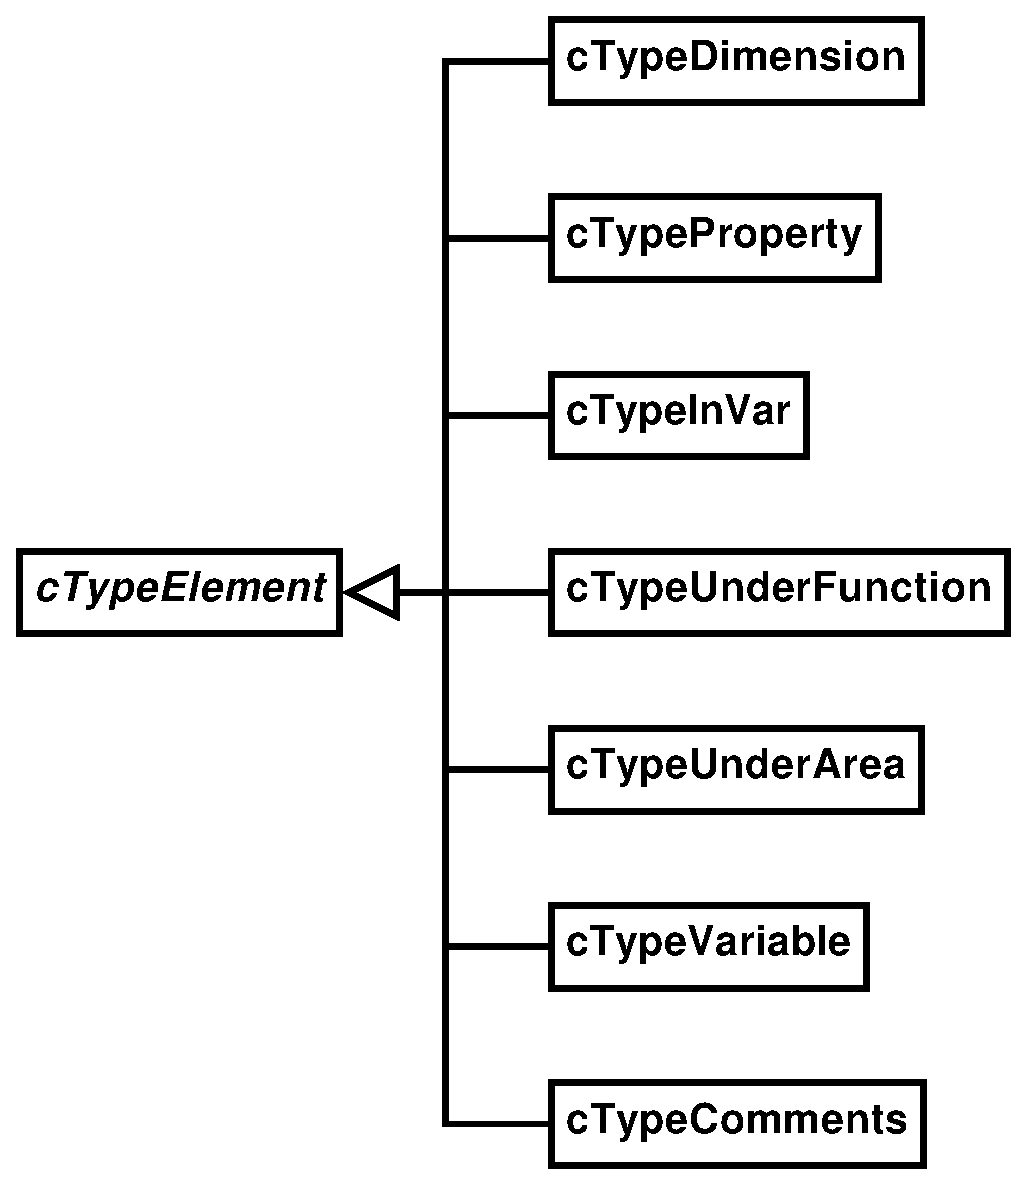
\includegraphics[scale=0.4]{fib_element_typen}
\end{center}
\caption{Klassengraph Fib-Elementtypen}
\label{figClassFibElementtyps}
\end{figure}

\subsubsection{getType}\index{cTypeElement!getType()}\index{getType()}

\textbf{Syntax:} \verb|unsignedIntFib getType()|

\bigskip\noindent
Diese Methode gibt eine Nummer f"ur den Typ des Elements zur"uck.

\bigskip\noindent
Die Nummern f"ur die Typen sind:
\begin{itemize}
 \item 1 f"ur cTypeDimension
 \item 2 f"ur cTypeSubarea
 \item 3 f"ur cTypeUnderFunction
 \item 5 f"ur cTypeInVar
 \item 6 f"ur cTypeProperty
 \item 10 f"ur cTypeVariable
 \item 11 f"ur cTypeComments
 \item 12 f"ur cTypeExternObject
 \item 13 f"ur cTypeExtSubobject
 \item 14 cTypeFibSet
 \item 15 cTypeFibMatrix
 \item 16 cTypeExtObjectInput
\end{itemize}

\bigskip\noindent
\textbf{Eingabeparameter:} keine

\bigskip\noindent
\textbf{R"uckgabe:} Der Typ des Vektors.


\subsubsection{isCompatible}\index{cTypeElement!isCompatible()}\index{isCompatible()}

\textbf{Syntax:} \verb|bool isCompatible( const cDomain & domain )|

\bigskip\noindent
Diese Methode gibt zur"uck, ob der Elemententyp kompatibel zum angegebenen Definitionsbereiche \verb|domain| ist.

\bigskip\noindent
\textbf{Eingabeparameter:}
\begin{itemize}
 \item \verb|domain|: Eine Referenz auf den Definitionsbereich, welcher kompatibel zum Typ des Elements sein soll.
\end{itemize}

\bigskip\noindent
\textbf{R"uckgabe:} Es wird \verb|true| (=wahr) zur"uckgegeben, wenn der Definitionsbereich \verb|domain| kompatibel ist, sonst \verb|false| (=falsch).


\subsubsection{getStandardDomain}\index{cTypeElement!getStandardDomain()}\index{getStandardDomain()}

\textbf{Syntax:} \verb|cDomain * getStandardDomain()|

\bigskip\noindent
Diese Methode gibt einen Zeiger auf den Standarddefinitionsbereich des Elemententyps zur"uck.

Das Objekt zum Standarddefinitionsbereich wird nicht automatisch gel"oscht. Das L"oschen des Objekts sollte also nach der Verwendung sichergestellt werden.

\bigskip\noindent
\textbf{Eingabeparameter:} keine

\bigskip\noindent
\textbf{R"uckgabe:} Zur"uckgegeben wird ein Zeiger auf den Standarddefinitionsbereich des Elemententyps.


\subsubsection{equalElementType}\index{cTypeElement!equalElementType()}\index{equalElementType()}

\textbf{Syntax:} \verb|bool equalElementType(| \\\verb| const cTypeElement & typeElement ) const|

\bigskip\noindent
Diese Methode pr"uft, ob der "ubergebene Elementtyp f"ur \verb|typeElement| mit dem aktuellen Elementtyp "ubereinstimmt. Zwei Elementtype stimmen "uberein, wenn sie zum gleichen Element geh"oren. Demnach darf es keine zwei Definitionsbereich zum gleichen Elementtyp gleichzeitig geben.

Der ein Positionselementtyp ist beispielsweise zu allen anderen m"oglichen Positionselementtypen gleich, unabh"angig von deren Dimension und Dimensionsmapping, da es nur eine Art von Positionsvektoren geben darf. Es gibt aber viele verschiedene Elementtypen f"ur die Eigenschaftstypen, da es f"ur verscheidene Eigenschaften verschiedene Vektoren geben kann.

\bigskip\noindent
\textbf{Eingabeparameter:}
\begin{itemize}
 \item \verb|typeElement|: Der Elementtyp, zu mit dem aktuelle Elementtyp "ubereinstimmt soll.
\end{itemize}

\bigskip\noindent
\textbf{R"uckgabe:} Wenn der aktuelle Elementtyp mit dem "ubergebenen \verb|typeElement| Elementtyp "ubereinstimmt, wird \verb|true| (=wahr) zur"uckgegeben, sonst wird \verb|false| (=falsch) zur"uckgegeben.


\subsubsection{equal}\index{cTypeElement!equal()}\index{equal()}

\textbf{Syntax:} \verb|bool equal( const cTypeElement & typeElement)const|

\noindent
\textbf{Syntax:} \verb|bool operator==( const cTypeElement & typeElement| \\\verb| ) const|

\bigskip\noindent
Diese Methode pr"uft, ob der "ubergebene Elementtyp \verb|typeElement| gleich zum aktuellen Elementtyp ist.

\bigskip\noindent
\textbf{Eingabeparameter:}
\begin{itemize}
 \item \verb|typeElement|: Der Elementtyp, zu dem der aktuelle Elementtyp gleich sein soll.
\end{itemize}

\bigskip\noindent
\textbf{R"uckgabe:} Wenn der aktuelle Elementtyp zum Elementtyp \verb|typeElement| gleich ist, wird \verb|true| (=wahr) zur"uckgegeben, sonst \verb|false| (=falsch).



\subsubsection{cTypeDimension}\index{cTypeElement!cTypeDimension}\index{cTypeDimension}

\textbf{Typ f"ur Element:} cVectorPosition; Die Nummer f"ur die Richtungen der Dimension werden "uber den Konstruktor bestimmt.

\bigskip\noindent
\textbf{Standarddefinitionsbereich:}

$vector( 2 , naturalNumberB(16), naturalNumberB(16) )$

\bigskip\noindent
\textbf{Kompatible Definitionsbereiche:} Vektoren

\bigskip\noindent
\textbf{Inkompatible Definitionsbereiche:} alle einzelnen Zahlen


\paragraph{Konstanten}

Folgende Konstanten werden von der Klasse \verb|cTypeDimension| definiert.

\begin{itemize}
 \item \verb|static const unsignedIntFib DIRECTION_NONE  = 0|
 \item \verb|static const unsignedIntFib DIRECTION_HORIZONTAL=1|
 \item \verb|static const unsignedIntFib DIRECTION_VERTICAL=2|
 \item \verb|static const unsignedIntFib DIRECTION_DEPTH = 3|
 \item \verb|static const unsignedIntFib DIRECTION_TIME  = 4|
\end{itemize}


\paragraph{cTypeDimension}

\ \\\\\noindent
\textbf{Syntax:} \verb|cTypeDimension(| \\\verb| unsigendIntFib iNumberOfDimensions=2 )|

\bigskip\noindent
Der Konstruktor des Dimensionstypobjekts, er erstellt einen Dimensionstypobjekt.

Den Dimensionen werden Initial die Werte 1 bis \verb|iNumberOfDimensions| zugeordnet, wie sie in Tabelle \ref{tableDimmapValues} auf Seite \pageref{tableDimmapValues} aufgef"uhrt sind. Bei zwei Dimensionen (Standardwert) w"are nach dem Erzeugen des Multimediainformationenobjekts die erste Dimension in Richtung ``horizontal'' und die zweite in Richtung ``vertikal''.

\bigskip\noindent
\textbf{Eingabeparameter:}
\begin{itemize}
 \item \verb|iNumberOfDimensions|: Die Anzahl der Dimensionen, welches das Fib-Objekt haben soll. Standardwert ist $2$ .
\end{itemize}

\bigskip\noindent
\textbf{R"uckgabe:} keine


\paragraph{cTypeDimension}

\ \\\\\noindent
\textbf{Syntax:} \verb|cTypeDimension(| \\\verb| vector<unsigendIntFib> vecDimensionsMapping )|

\bigskip\noindent
Der Konstruktor des Dimensionstypobjekts, er erstellt einen Dimensionstypobjekt.

\bigskip\noindent
\textbf{Eingabeparameter:}
\begin{itemize}
 \item \verb|vecDimensionsMapping|: Der Vektor mit den Mappingwerten f"ur die Dimensionen. Die Werte werden in Tabelle \ref{tableDimmapValues} auf Seite \pageref{tableDimmapValues} definiert. Der $i$'te Vektorwert steht f"ur die $i+1$'te Dimension. "Uber diesen Vektor wird auch die Anzahl der Dimensionen bestimmt. Wiederholt auftauchende Mappingwerte werden auf den Mappingwert $0$ f"ur ``none'' gesetzt.
\end{itemize}

\bigskip\noindent
\textbf{R"uckgabe:} keine


\paragraph{getNumberOfDimensions}\index{cTypeDimension!getNumberOfDimensions()}\index{getNumberOfDimensions()}

\ \\\\\noindent
\textbf{Syntax:} \verb|unsigendIntFib getNumberOfDimensions() const|

\bigskip\noindent
Diese Methode gibt die Anzahl der Dimensionen zur"uck, f"ur welche das Objekt steht.

\bigskip\noindent
\textbf{Eingabeparameter:} keine

\bigskip\noindent
\textbf{R"uckgabe:} Die Anzahl der Dimension, f"ur welche das Objekt steht.


\paragraph{getDimensionMapping}\index{cTypeDimension!getDimensionMapping()}\index{getDimensionMapping()}

\ \\\\\noindent
\textbf{Syntax:} \verb|unsignedIntFib getDimensionMapping(| \\\verb| unsignedIntFib iDimensionNumber ) const|

\bigskip\noindent
Diese Methode gibt den Mappingwert f"ur die Dimension \verb|iDimensionNumber| zur"uck. Existiert keine solche Dimension, wird $0$ f"ur \verb|none| zur"uckgegeben.

Die Werte werden in Tabelle \ref{tableDimmapValues} auf Seite \pageref{tableDimmapValues} definiert.

\bigskip\noindent
\textbf{Eingabeparameter:}
\begin{itemize}
 \item \verb|iDimensionNumber|: Nummer der Dimension, f"ur welche der Mappingwert zur"uckgegeben werden soll.
\end{itemize}

\bigskip\noindent
\textbf{R"uckgabe:} Den Mappingwert f"ur die Dimension \verb|iDimensionNumber|, existiert keine solche Dimension wird $0$ zur"uckgegeben.


\paragraph{setDimensionMapping}\index{cTypeDimension!setDimensionMapping()}\index{setDimensionMapping()}

\ \\\\\noindent
\textbf{Syntax:} \verb|bool setDimensionMapping(| \\\verb| unsignedIntFib iDimensionNumber,| \\\verb| unsignedLongFib lMapping )|

\bigskip\noindent
Diese Methode setzt den Mappingwert f"ur die Dimension \verb|iDimensionNumber|.
Die Werte werden in Tabelle \ref{tableDimmapValues} auf Seite \pageref{tableDimmapValues} definiert.

Wird versucht ein Mapping einzustellen, auf welches schon ein anderen Dimension gesetzt ist, wird das Mapping nicht ge"andert und \verb|false| (=falsch) zur"uckgegeben. Jede Dimension kann allerdings immer auf 0 (=kein Mapping) gesetzt werden.

Wenn kein entsprechendes \verb|iDimensionNumber|'tes Dimensionsmapping ex\-is\-tiert, wird \verb|false| (=falsch) zur"uckgegeben.

\bigskip\noindent
\textbf{Eingabeparameter:}
\begin{itemize}
 \item \verb|iDimensionNumber|: Nummer der Dimension, f"ur welche das Mapping ge"andert werden soll.
 \item \verb|lMapping|: Neuer Wert f"ur das Mapping der Dimension.
\end{itemize}

\bigskip\noindent
\textbf{R"uckgabe:} Es wird \verb|true| (=wahr) zur"uckgegeben, wenn das Mappingwert gesetzt wurden, sonst \verb|false| (=falsch).


\paragraph{getDimensionMappingName}\index{cTypeDimension!getDimensionMappingName()}\index{getDimensionMappingName()}

\ \\\\\noindent
\textbf{Syntax:} \verb|static string getDimensionMappingName(| \\\verb| unsignedLongFib ulMapping )|

\bigskip\noindent
Diese Methode liefert Namen f"ur den den Mappingwert \verb|ulMapping|.
Die Werte und Namen werden in Tabelle \ref{tableDimmapValues} auf Seite \pageref{tableDimmapValues} definiert und einander zugeordnet.


\bigskip\noindent
\textbf{Eingabeparameter:}
\begin{itemize}
 \item \verb|ulMapping|: Der Wert f"ur das Mapping, f"ur welche der Name zur"uckgegeben werden soll.
\end{itemize}

\bigskip\noindent
\textbf{R"uckgabe:} Den Namen f"ur den Mappingwert \verb|ulMapping|.


\paragraph{getUnit}\index{cTypeDimension!getUnit()}\index{getUnit()}

\ \\\\\noindent
\textbf{Syntax:} \verb| vector<string> getUnit() const|

\bigskip\noindent
Diese Methode gibt einen Vektor mit den Zeichenketten mit den (SI-) Einheiten f"ur die Vektorelemente/Dimensionen des Typs zur"uck.

Ist eine Einheit unbekannt (bzw. die Eigenschaft ist kein Standardtyp), wird eine leere Zeichenkette f"ur sie zur"uckgegeben.

\bigskip\noindent
\textbf{Eingabeparameter:} keine

\bigskip\noindent
\textbf{R"uckgabe:} Einen Vektor mit den Zeichenketten mit den (SI-) Einheiten f"ur die Vektorelemente des Typ.



\subsubsection{cTypeArea}\index{cTypeElement!cTypeArea}\index{cTypeArea}

\textbf{Typ f"ur Element:} cArea%; Die obere und untere Grenze f"ur die Unterbereiche.

\bigskip\noindent
\textbf{Standarddefinitionsbereich:} $vector( 2, naturalNumberB(8),$ $vector( 2,$ $integerB(16),$ $integerB(16) ) )$


Dieser Typ ist f"ur Definitionsbereich f"ur das Bereichselement (siehe Abschnitt \ref{fibArea} auf Seite \pageref{fibArea} und Abschnitt \ref{secCompressedArea} auf Seite \pageref{secCompressedArea}) im Haupt-Fib-Objekt. Der zugeh"orige Definitionsbereich ist ein Vektordefinitionsbereich mit 2 Elementen /Unterdefinitionsbereichen. Das erste Element bzw. der erste Unterdefinitionsbereich dient f"ur die Anzahl ($n$) der Unterbereiche, er ist ein Definitionsbereich aus den nat"urlichen Zahlen. Das zweite und letzte Element ist der Definitionsbereich f"ur die Vektoren f"ur die Unterbereiche ($B_{1}$) und ist ein Definitionsbereich f"ur Vektoren dessen zwei Elemente ganze Zahlen sind. 

\bigskip\noindent
\textbf{Kompatible Definitionsbereiche:} alle Vektoren mit zwei Elementen, deren erstes Element nat"urliche Zahlen ist und deren zweites Element ein Vektor mit zwei ganzen Zahlen ist

\bigskip\noindent
\textbf{Inkompatible Definitionsbereiche:} alle einzelnen Zahlen, alle Vektoren mit nicht zwei Unterdefinitionsbereichen und Vektoren in denen das erstes Element keine nat"urliche Zahlen ist oder der zweite Unterdefinitionsbereich kein Vektor mit zwei ganzen Zahlen ist


\subsubsection{cTypeUnderFunction}\index{cTypeElement!cTypeUnderFunction}\index{cTypeUnderFunction}

\textbf{Typ f"ur Element:} cUnderFunction; Die Zahlen in Funktionen.

\bigskip\noindent
\textbf{Standarddefinitionsbereich:} $naturalNumberB(16)$

\bigskip\noindent
\textbf{Kompatible Definitionsbereiche:} alle einzelnen Zahlen

\bigskip\noindent
\textbf{Inkompatible Definitionsbereiche:} Vektoren


\subsubsection{cTypeInVar}\index{cTypeElement!cTypeInVar}\index{cTypeInVar}

\textbf{Typ f"ur Element:} Eingabevariable $inVar_i$; Die Nummer der Eingabevariable wird "uber den Konstruktor bestimmt. Nur Eingabevariablen des aktuellen root-Elements k"onnen hier auftauchen.

\bigskip\noindent
\textbf{Standarddefinitionsbereich:} $naturalNumberB(16)$

\bigskip\noindent
\textbf{Kompatible Definitionsbereiche:} alle einzelnen Zahlen

\bigskip\noindent
\textbf{Inkompatible Definitionsbereiche:} Vektoren


\paragraph{cTypeInVar}

\ \\\\\noindent
\textbf{Syntax:} \verb|cTypeInVar( unsignedIntFib iNumberInputVariable )|

\bigskip\noindent
Der Konstruktor des Eingabevariablentypobjekts, er erstellt einen Eingabevariablentypobjekt.

\bigskip\noindent
\textbf{Eingabeparameter:}
\begin{itemize}
 \item \verb|iNumberInputVariable|: Die Nummer der Eingabevariable, f"ur welche das Objekt steht.
\end{itemize}

\bigskip\noindent
\textbf{R"uckgabe:} keine


\paragraph{getNumberOfInputVariable}\index{cTypeInVar!getNumberOfInputVariable()}\index{getNumberOfInputVariable()}

\ \\\\\noindent
\textbf{Syntax:} \verb|unsignedIntFib getNumberOfInputVariable() const|

\bigskip\noindent
Diese Methode gibt die Nummer der Eingabevariable zur"uck, f"ur das das Objekt steht.

\bigskip\noindent
\textbf{Eingabeparameter:} keine

\bigskip\noindent
\textbf{R"uckgabe:} Die Nummer der Eingabevariable, f"ur welche das Objekt steht.



\subsubsection{cTypeProperty}\index{cTypeElement!cTypeProperty}\index{cTypeProperty}

\textbf{Typ f"ur Element:} cVectorProperty; Der Typ der Eigenschaft wird "uber den Konstruktor bestimmt.

\bigskip\noindent
\textbf{Standarddefinitionsbereich:} $vector( 1 , naturalNumberB(16) )$

F"ur einige Eigenschaften ist der Standarddefinitionsbereich des Eigenschaftsvektors von $vector( 1 , naturalNumberB(16) )$ abweichend. In Tabelle \ref{tableElementsForDomains} auf Seite \pageref{tableElementsForDomains} sind die abweichenden Standarddefinitionsbereiche aufgef"uhrt.

\bigskip\noindent
\textbf{Kompatible Definitionsbereiche:} Vektoren deren Elemente einzelnen Zahlen sind

\bigskip\noindent
\textbf{Inkompatible Definitionsbereiche:} alle einzelnen Zahlen


\paragraph{Konstanten}

Folgende Konstanten werden von der Klasse \verb|cTypeProperty| definiert:

\begin{itemize}
 \item \verb|static const unsignedIntFib COLOR_RGB = 1|
 \item \verb|static const unsignedIntFib COLOR_SW  = 2|
 \item \verb|static const unsignedIntFib LAYER     = 100|
 \item \verb|static const unsignedIntFib TRANSPARENCY    = 200|
 \item \verb|static const unsignedIntFib SOUND     = 300|
 \item \verb|static const unsignedIntFib SOUND_POLARIZED = 301|
 \item \verb|static const unsignedIntFib SOUND_AMPLITUDE = 305|
 \item \verb|static const unsignedIntFib SOUND_BARRIER   = 310|
 \item \verb|static const unsignedIntFib SOUND_REFLECTED = 311|
 \item \verb|static const unsignedIntFib SOUND_DAMPING   = 312|
 \item \verb|static const unsignedIntFib KELVIN    = 400|
 \item \verb|static const unsignedIntFib ELECTRO_MAGNETIC= 410|
\end{itemize}


\paragraph{cTypeProperty}\index{cTypeElement!cTypeProperty}

\ \\\\\noindent
\textbf{Syntax:} \verb|cTypeProperty( intFib iTypeProperty )|

\bigskip\noindent
Der Konstruktor des Eigenschaftstypobjekts, er erstellt einen Eigenschaftstypobjekt.

Die Nummer des Eigenschaftstyps sind die Werte aus Tabelle \ref{tablePropertyNamen} auf Seite \pageref{tablePropertyNamen} .

\bigskip\noindent
\textbf{Eingabeparameter:}
\begin{itemize}
 \item \verb|iTypeProperty|: Die Nummer des Typs, der Eigenschaft f"ur das das Objekt steht. Die m"oglichen Werte f"ur die unterschiedlichen Eigenschaften sind aus Tabelle \ref{tablePropertyNamen} auf Seite \pageref{tablePropertyNamen} aus der Spalte ``Wert'' zu entnehmen.
\end{itemize}

\bigskip\noindent
\textbf{R"uckgabe:} keine


\paragraph{cTypeProperty}

\ \\\\\noindent
\textbf{Syntax:} \verb|cTypeProperty( unsignedIntFib uiPropertyType,| \\\verb| unsignedIntFib uiNumberOfDimensions=2 )|

\bigskip\noindent
Der Konstruktor des Eigenschaftstypobjekts, er erstellt einen Eigenschaftstypobjekts.

\bigskip\noindent
\textbf{Eingabeparameter:}
\begin{itemize}
 \item \verb|uiPropertyType|: Die Nummer der Eigenschaft, f"ur welche das Objekt steht.
 \item \verb|uiNumberOfDimensions|: Die Nummer der der Dimensionen der Eigenschaft. Bei manche Eigenschaften ist die Anzahl der Element von der Dimension abh"angig (z.B $soundPolarized$), deshalb wird diee Angabe ben"otigt.
\end{itemize}

\bigskip\noindent
\textbf{R"uckgabe:} keine


\paragraph{getNumberOfProperty}\index{cTypeProperty!getNumberOfProperty()}\index{getNumberOfProperty()}

\ \\\\\noindent
\textbf{Syntax:} \verb|unsignedIntFib getNumberOfProperty()|

\bigskip\noindent
Diese Methode gibt die Nummer der Eigenschaft zur"uck, f"ur welche das Objekt steht.
In Tabelle \ref{tablePropertyNamen} auf Seite \pageref{tablePropertyNamen} sind die Nummern der Eigenschaften ind der Spalte ``Wert'' aufgef"uhrt.

\bigskip\noindent
\textbf{Eingabeparameter:} keine

\bigskip\noindent
\textbf{R"uckgabe:} Die Nummer der Eigenschaft f"ur das das Objekt steht.


\paragraph{getNumberOfProperty}\index{cTypeProperty!getNumberOfProperty()}\index{getNumberOfTypeProperty()}

\ \\\\\noindent
\textbf{Syntax:} \verb|intFib getNumberOfTypeProperty() const|

\bigskip\noindent
Diese Methode gibt die Nummer des Typs der Eigenschaft zur"uck, f"ur welchen das Objekt steht.

Die Nummer des Eigenschaftstyps sind die Werte aus Tabelle \ref{tablePropertyNamen} auf Seite \pageref{tablePropertyNamen} in der Spalte ``Wert'' aufgef"uhrt.

\bigskip\noindent
\textbf{Eingabeparameter:} keine

\bigskip\noindent
\textbf{R"uckgabe:} Die Nummer der des Typs der Eigenschaft, f"ur welche das Objekt steht.


\paragraph{getUnit}\index{cTypeProperty!getUnit()}\index{getUnit()}

\ \\\\\noindent
\textbf{Syntax:} \verb|vector<string> getUnit() const|

\bigskip\noindent
Diese Methode gibt einen Vektor mit den Zeichenketten mit den (SI-) Einheiten f"ur die Vektorelemente des Typs zur"uck.

Ist eine Einheit unbekannt (bzw. die Eigenschaft ist kein Standardtyp), wird eine leere Zeichenkette f"ur sie zur"uckgegeben.

\bigskip\noindent
\textbf{Eingabeparameter:} keine

\bigskip\noindent
\textbf{R"uckgabe:} Einen Vektor mit den Zeichenketten mit den (SI-) Einheiten f"ur die Vektorelemente des Eigenschaftstyps.



\subsubsection{cTypeVariable}\index{cTypeElement!cTypeVariable}\index{cTypeVariable}

\textbf{Typ f"ur Element:} cVariable

\bigskip\noindent
\textbf{Standarddefinitionsbereich:} $naturalNumberB(8)$

Der zugeh"orige Definitionsbereich dient f"ur die Werte die ben"otigt werden, um Variablen im komprimierten Speicherformat zu kodieren. Der Definitionsbereich sollten die nat"urliche Zahlen von 0 bis maximale Anzahl der definierten Variablen in den Fib-Bl"attern im Haupt-Fib-Objekt sein. Das Fib-Baum-Blatt im Haupt-Fib-Objekt "uber dem meisten Variablen definiert werden, bestimmt also den Definitionsbereich, bzw. der Ast mit den meisten definierten Variablen. Dieser Eintrag wird beim Abspeichern erstellt.

\bigskip\noindent
\textbf{Kompatible Definitionsbereiche:} alle nat"urlichen, unskalierte Zahlen

\bigskip\noindent
\textbf{Inkompatible Definitionsbereiche:} alle einzelnen Zahlen die nicht nat"urlichen, unskalierte Zahlen sind und alle Vektoren



\subsubsection{cTypeComments}\index{cTypeElement!cTypeComments}\index{cTypeComments}

\textbf{Typ f"ur Element:} cComment

\bigskip\noindent
\textbf{Standarddefinitionsbereich:} $naturalNumberB(8)$

Der zugeh"orige Definitionsbereich dient f"ur die Werte die ben"otigt werden, um Kommentare im komprimierten Speicherformat zu kodieren. Der Definitionsbereich sollten die nat"urliche Zahlen von 0 bis Anzahl der Kommentare im Haupt-Fib-Objekt sein. Dieser Eintrag wird beim Abspeichern erstellt.

\bigskip\noindent
\textbf{Kompatible Definitionsbereiche:} alle nat"urlichen, unskalierte Zahlen

\bigskip\noindent
\textbf{Inkompatible Definitionsbereiche:} alle einzelnen Zahlen die nicht nat"urlichen, unskalierte Zahlen sind und alle Vektoren


\subsubsection{cTypeExtObjekt}\index{cTypeElement!cTypeExtObjekt}\index{cTypeExtObjekt}

\textbf{Typ f"ur Element:} cExtObjekt

\bigskip\noindent
\textbf{Standarddefinitionsbereich:}

$vector( 4 , integerB(32), naturalNumberB(4), naturalNumberB(2),$

$naturalNumberB(2) )$

Dieser Typ ist f"ur Definitionsbereich f"ur externe Objekte im Haupt-Fib-Objekt. Der Definitionsbereich ist ein Vector mit 4 Elementen. Die Vektorelemente dienen der Reihenfolge f"ur den Identifier, die Anzahl der Eingabevariablen NumberInVar, die Anzahl der Unterobjekte NumberUnderObjects und die Anzahl der Ausgabevariablen NumberOutVar. Alle Vektorelementdefinitionsbereiche, au"ser dem f"ur den Identifier, kommen aus den nat"urlichen Zahlen. Der Vektorelementdefinitionsbereich f"ur den Identifier kommt aus den Ganzzahlen. Dieser Definitionsbereich wird normalerweise beim Abspeichern erstellt.

\bigskip\noindent
\textbf{Kompatible Definitionsbereiche:} Vektoren mit 4 Elementen deren erstes Elemente eine einzelnen Ganzzahlen ist und dessen anderen Elemente nat"urliche Zahlen sind, alle Vektorelemente sind unskaliert

\bigskip\noindent
\textbf{Inkompatible Definitionsbereiche:} alle einzelnen Zahlen, alle Vektoren die nicht kompatible sind


\subsubsection{cTypeExtObjectInput}\index{cTypeElement!cTypeExtObjectInput}\index{cTypeExtObjectInput}

\textbf{Typ f"ur Element:} Eingabewerte von externen Objekten (cExtObjekt); Der Identifier des externen Objekts wird "uber den Konstruktor bestimmt.

\bigskip\noindent
\textbf{Standarddefinitionsbereich:} $vectorOpenEnd( integerB(8) )$

\bigskip\noindent
\textbf{Kompatible Definitionsbereiche:} Vektoren deren Elemente einzelnen Zahlen sind

\bigskip\noindent
\textbf{Inkompatible Definitionsbereiche:} alle einzelnen Zahlen


\paragraph{cTypeExtObjectInput}

\ \\\\\noindent
\textbf{Syntax:} \verb|cTypeExtObjectInput( long lIdentifier )|

\bigskip\noindent
Der Konstruktor des Eingabewertetypobjekts f"ur externen Objekten, er erstellt einen Eingabewertetypobjekt f"ur externen Objekten mit dem Identifier lIdentifier.

\bigskip\noindent
\textbf{Eingabeparameter:}
\begin{itemize}
 \item \verb|lIdentifier|: Der Identifier des externen Objekts, f"ur welche das Objekt steht.
\end{itemize}

\bigskip\noindent
\textbf{R"uckgabe:} keine


\paragraph{getIdentifier}\index{cTypeExtObjectInput!getIdentifier()}\index{getIdentifier()}

\ \\\\\noindent
\textbf{Syntax:} \verb|long getIdentifier() const|

\bigskip\noindent
Diese Methode gibt den Identifier des externen Objekts zur"uck, f"ur dessen Eingabewerte das Objekt steht.

\bigskip\noindent
\textbf{Eingabeparameter:} keine

\bigskip\noindent
\textbf{R"uckgabe:} Die Identifier des externen Objekts, f"ur dessen Eingabewerte das Objekt steht.



\subsubsection{cTypeExtSubobject}\index{cTypeElement!cTypeExtSubobject}\index{cTypeExtSubobject}

\textbf{Typ f"ur Element:} f"ur das externe Subobjekt (cExtSubobject); Die Nummer des externen Subobjekts wird "uber den Konstruktor bestimmt. Nur externe Subobjekte des Haup-Fib-Objects des aktuellen root-Elements k"onnen hier auftauchen.

\bigskip\noindent
\textbf{Standarddefinitionsbereich:} $vector( 0 )$

\bigskip\noindent
\textbf{Kompatible Definitionsbereiche:} Vektoren deren Elemente einzelnen Zahlen sind

\bigskip\noindent
\textbf{Inkompatible Definitionsbereiche:} alle einzelnen Zahlen


\paragraph{cTypeExtSubobject}

\ \\\\\noindent
\textbf{Syntax:} \verb|cTypeExtSubobject( const unsignedIntFib iNumberExtSubobject )|

\bigskip\noindent
Der Konstruktor des externen Subobjekt Typs, er erstellt einen externe Subobjekt Type.

\bigskip\noindent
\textbf{Eingabeparameter:}
\begin{itemize}
 \item \verb|iNumberExtSubobject|: Die Nummer des externen Subobjekts, f"ur welche das Objekt steht.
\end{itemize}

\bigskip\noindent
\textbf{R"uckgabe:} keine


\paragraph{getNumberOfExtSubobject}\index{cTypeExtSubobject!getNumberOfExtSubobject()}\index{getNumberOfExtSubobject()}

\ \\\\\noindent
\textbf{Syntax:} \verb|unsignedIntFib getNumberOfExtSubobject() const|

\bigskip\noindent
Diese Methode gibt die Nummer des externen Subobjekts zur"uck, f"ur das das Objekt steht.

\bigskip\noindent
\textbf{Eingabeparameter:} keine

\bigskip\noindent
\textbf{R"uckgabe:} Die Nummer der externen Subobjekts, f"ur welche das Objekt steht.



% TODO weg:
% \subsubsection{cTypeExtSubobject}\index{cTypeElement!cTypeExtSubobject}\index{cTypeExtSubobject}
% 
% \textbf{Typ f"ur Element:} cExtSubobject
% 
% \bigskip\noindent
% \textbf{Standarddefinitionsbereich:} $naturalNumberB(4)$
% 
% Der zugeh"orige Definitionsbereich dient f"ur die Anzahl der Eingebevariablen f"ur externe Unterobjekte. Der Definitionsbereich ist immer eine Untermenge der nat"urlichen Zahlen und wird normalerweise beim Abspeichern erstellt.
% 
% \bigskip\noindent
% \textbf{Kompatible Definitionsbereiche:} alle nat"urlichen, unskalierte Zahlen
% 
% \bigskip\noindent
% \textbf{Inkompatible Definitionsbereiche:} alle einzelnen Zahlen die nicht nat"urlichen, unskalierte Zahlen sind und alle Vektoren




\subsubsection{cTypeFibSet}\index{cTypeElement!cTypeFibSet}\index{cTypeFibSet}

\textbf{Typ f"ur Element:} cTypeFibSet

\bigskip\noindent
\textbf{Standarddefinitionsbereich:} $vector( 3, naturalNumberB(8),$ $naturalNumberB(32),$ $vectorOpenEnd( 1,$ $integerB(32) ) )$

Dieser Typ ist f"ur Definitionsbereich f"ur das set-Element (siehe Abschnitt \ref{secFibSetElement} auf Seite \pageref{secFibSetElement} und Abschnitt \ref{secCFibSetElement} auf Seite \pageref{secCFibSetElement}) im Haupt-Fib-Objekt. Der Definitionsbereich ist ein Vector mit 3 Elementen.  Das erste Element bzw. der erste Unterdefinitionsbereich dient f"ur die Anzahl ($n$) der Variablen und der zu setzenden Werte pro Satz, er ist ein Definitionsbereich aus den nat"urlichen Zahlen. Das zweite Element bzw. der zweite Unterdefinitionsbereich dient f"ur die Anzahl ($k$) der S"atze mit zu setzenden Werten. Er ist auch ein Definitionsbereich aus den nat"urlichen Zahlen. Das dritte und letzte Element ist der Definitionsbereich f"ur die Vektoren f"ur die zu setzenden Werte ($W_{i.g}$) und ist ein Definitionsbereich f"ur Vektoren deren Elemente einfache Zahlen (skalare) sind.

\bigskip\noindent
\textbf{Kompatible Definitionsbereiche:} alle Vektoren mit drei Elementen, deren ersten beiden Elemente nat"urliche Zahlen sind und deren drittes Element ein beliebiger Vektor mit Zahlen ist

\bigskip\noindent
\textbf{Inkompatible Definitionsbereiche:} alle einzelnen Zahlen, alle Vektoren mit nicht drei Unterdefinitionsbereichen und Vektoren in denen die ersten beiden Elemente keine nat"urliche Zahlen sind oder der dritte Unterdefinitionsbereich kein Vektor von Zahlen ist


\subsubsection{cTypeFibMatrix}\index{cTypeElement!cTypeFibMatrix}\index{cTypeFibMatrix}

\textbf{Typ f"ur Element:} cTypeFibMatrix

\bigskip\noindent
\textbf{Standarddefinitionsbereich:} $vector( 4, naturalNumberB(8),$ $naturalNumberB(32),$ $vector( 2 , integerB(16), integerB(16) )$, $vectorOpenEnd( 1,$ $integerB(32) ) )$

Dieser Typ ist f"ur Definitionsbereich f"ur das Matrixelement (siehe Abschnitt \ref{secFibMatrixElement} auf Seite \pageref{secFibMatrixElement} und Abschnitt \ref{secCFibMatrixElement} auf Seite \pageref{secCFibMatrixElement}) im Haupt-Fib-Objekt. Der Definitionsbereich ist ein Vector mit 4 Elementen.  Das erste Element bzw. der erste Unterdefinitionsbereich ist f"ur die Anzahl ($d$) der Dimensionsvariablen, die Anzahl ($i$) der Wertevariablen und die zu setzenden Werte $i$ pro Satz. Er ist ein Definitionsbereich aus den nat"urlichen Zahlen. Das zweite Element bzw. der zweite Unterdefinitionsbereich ist f"ur die Anzahl ($k$) der S"atze mit den zu setzenden Werten. Er ist auch ein Definitionsbereich aus den nat"urlichen Zahlen. Das dritte Element ist der Definitionsbereich f"ur die Bereiche bzw. Start und Endwerte f"ur die einzellenen Dimensionsvariablen, er ist ein Vektordefinitionsbereich mit zwei Elementen, welche jeweils aus den ganzen Zahlen kommen. Das vierte und letzte Element ist der Definitionsbereich f"ur die Vektoren f"ur die zu setzenden Werte ($W_{a.b}$) und ist ein Definitionsbereich f"ur Vektoren deren Elemente einfache Zahlen (skalare) sind.

\bigskip\noindent
\textbf{Kompatible Definitionsbereiche:} alle Vektoren mit vier Elementen, deren ersten beiden Elemente nat"urliche Zahlen sind, deren drittes Element ein Vektor mit zwei Ganzzahlen und deren viertes Element ein beliebiger Vektor mit Zahlen ist

\bigskip\noindent
\textbf{Inkompatible Definitionsbereiche:} alle einzelnen Zahlen, alle Vektoren mit nicht vier Unterdefinitionsbereichen und Vektoren in denen die ersten beiden Elemente keine nat"urliche Zahlen sind, Vektoren in denen der dritte Unterdefinitionsbereich kein Vektor von zwei Ganzzahlen ist oder der vierte Unterdefinitionsbereich kein Vektor von Zahlen ist



\subsection{Definitionsbereiche cDomain}\index{root-Element!Definitionsbereiche}\index{cDomains!cDomain}\index{cDomain}

Definitionsbereiche dienen zur Eingrenzung der m"oglichen Werte, welche ein Element einnehmen kann.

Es gibt zwei gro"se Klassen von Definitionsbereichen: Vektoredefinitionsbereiche und Definitionsbereiche f"ur einzelne (skalare) Werte/ Zahlen.

In Diagramm \ref{figClassFibDomains} ist eine Klassenhierarchie der Definitionsbereiche dargestellt.

\begin{figure}[htbp]
\begin{center}
  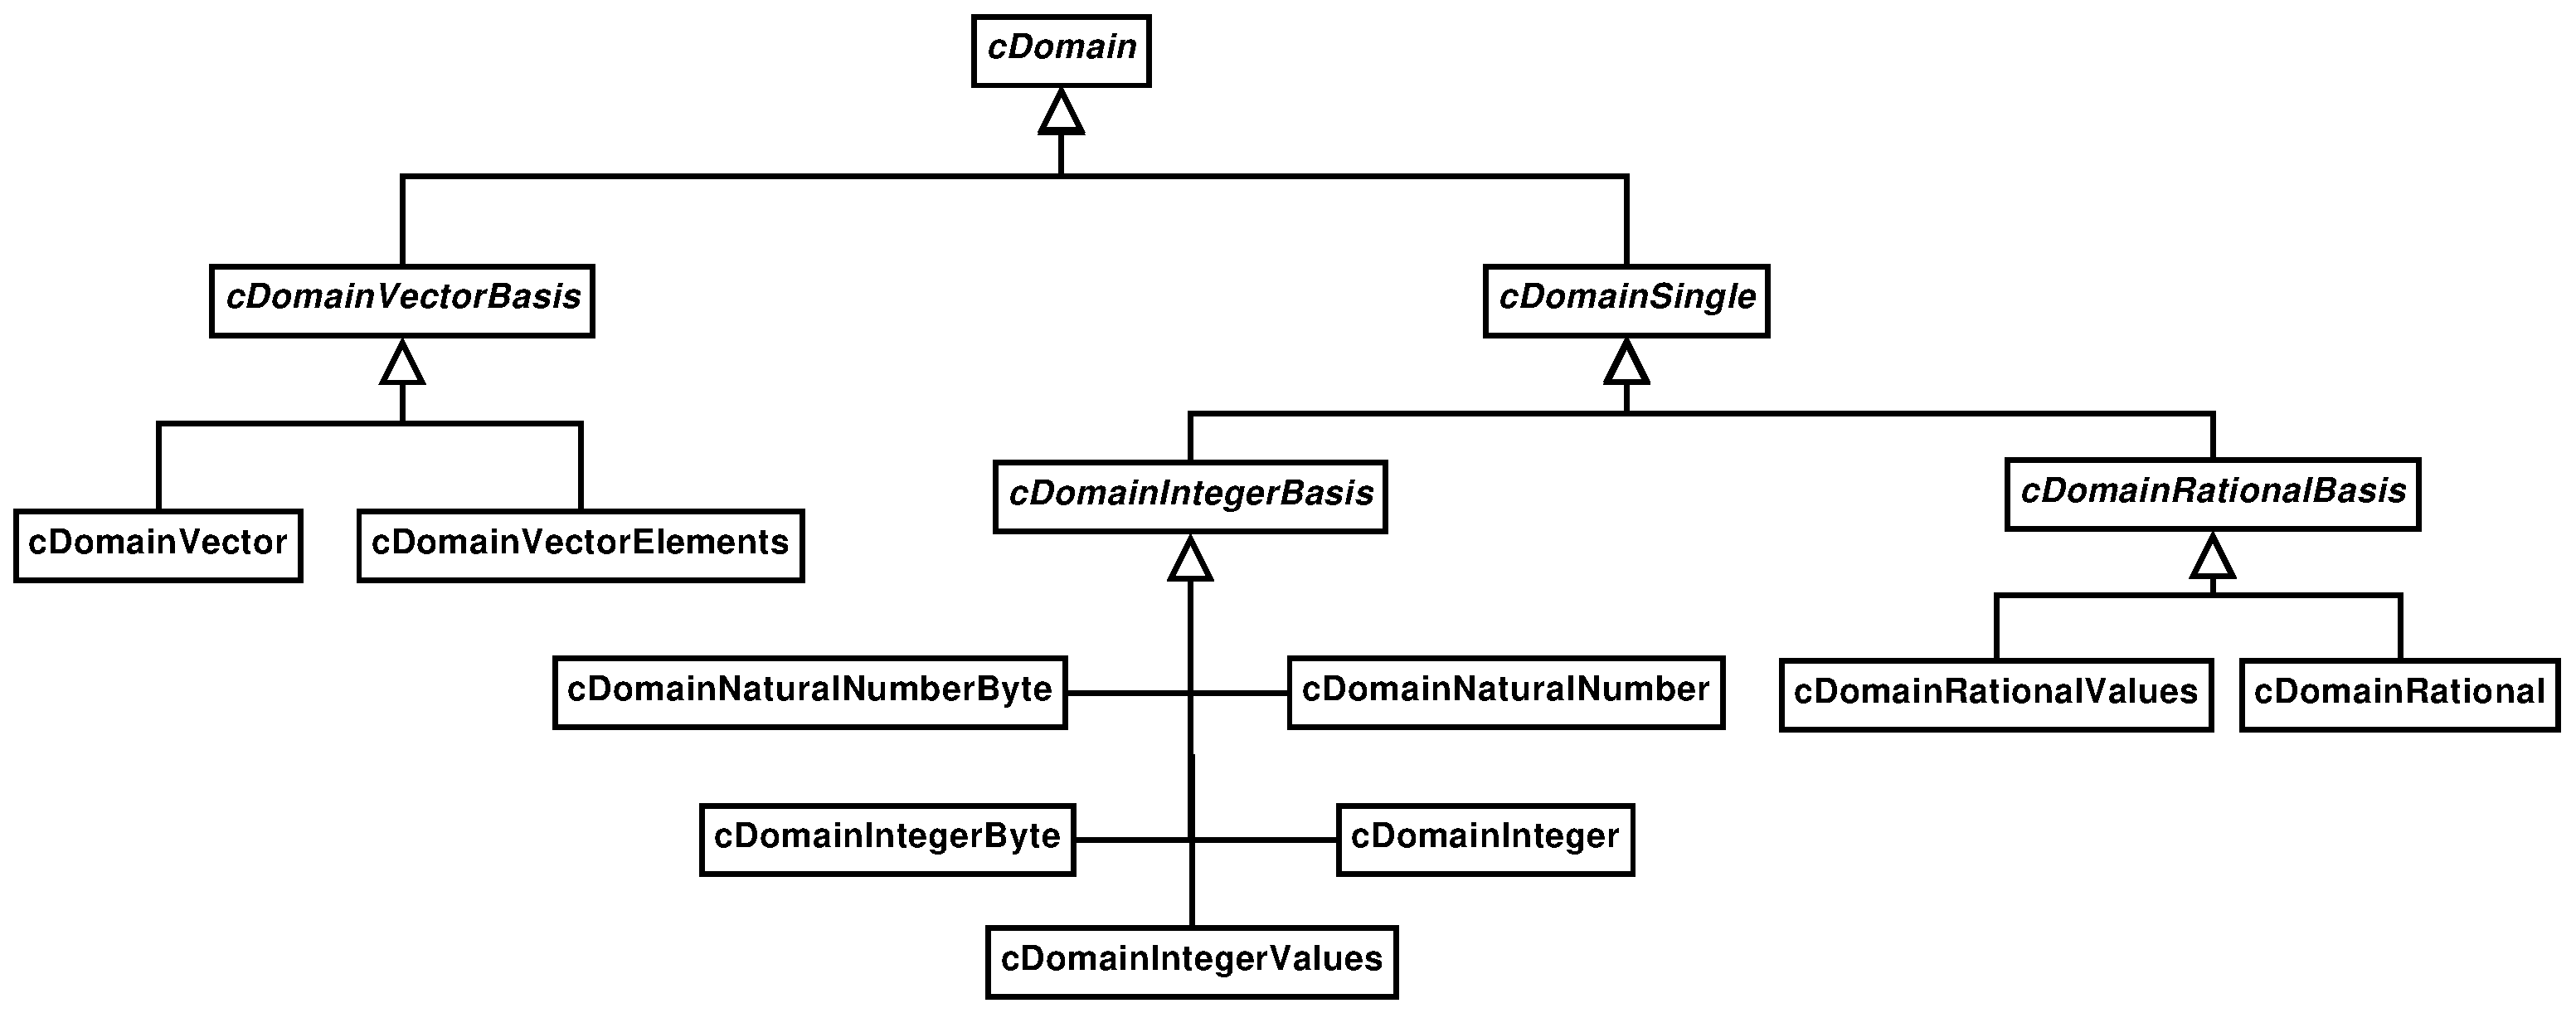
\includegraphics[scale=0.25]{fib_definition_areas}
\end{center}
\caption{Klassengraph der Fib-Definitionsbereiche}
\label{figClassFibDomains}
\end{figure}


\subsubsection{getType}\index{cDomain!getType()}\index{getType()}

\textbf{Syntax:} \verb|string getType()|

\bigskip\noindent
Diese Methode gibt den Typ des Definitionsbereichs als Zeichenkette zur"uck. Dies ist der Klassenname ohne das vorangestellte Zeichen ``c''. Beispielsweise geben Objekte der Klasse \verb|cDomainNaturalNumberBit| die Zeichenkette ``DomainNaturalNumberBit'' als Typ zur"uck.

\bigskip\noindent
\textbf{Eingabeparameter:} keine

\bigskip\noindent
\textbf{R"uckgabe:} Zur"uckgegeben wird der Typ des Definitionsbereichs als Zeichenkette.



\subsection{Einfache Definitionsbereiche cDomainSingle}\index{cDomain!cDomainSingle}\index{cDomainSingle}

Die Klasse \verb|cDomainSingle| ist der Basisklasseh aller einzelnen Zahlen (Skalare). Von \verb|cDomainSingle| werden alle Definitionsbereiche f"ur einfache Zahlen abgeleitet. Von \verb|cDomainSingle| selbst kann jedoch keine Instanz erzeugt werden.

Nach den folgenden Methoden der Klasse \verb|cDomainSingle| sind die von ihr abgeleiteten Klassen aufgef"uhrt.


\subsubsection{isElement}\index{cDomainSingle!isElement()}\index{isElement()}

\textbf{Syntax:} \verb|bool isElement( const doubleFib dValue ) const|

\bigskip\noindent
Diese Methode pr"uft, ob der "ubergebene Wert \verb|dValue| im (skalierten) Definitionsbereich liegt.

Diese Methode ist mit Vorsicht zu verwenden, da aufgrund von Rundungsfehlern bei Gleitkommawerten (\verb|doubleFib|) diese leicht voneinander abweichen k"onnen. F"ur Werte die von der \verb|round()| Methode zur"uckgegeben werden, gibt die \verb|isElement()| Methode \verb|true| (=wahr) zur"uck. Wenn aber beispielsweise zum R"uckgabewert $W$ der \verb|round()| Methode $3$ addiert und wieder abgezogen wird ($W+3-3$), ist das Ergebnis der \verb|isElement()| Methode unbestimmt.

\bigskip\noindent
\textbf{Eingabeparameter:}
\begin{itemize}
 \item \verb|dValue|: Der Wert, f"ur den zu pr"ufen ist, ob er im Definitionsbereich liegt.
\end{itemize}

\bigskip\noindent
\textbf{R"uckgabe:} Wenn der "ubergebene Wert \verb|dValue| im Definitionsbereich liegt, wird \verb|true| (=wahr) zur"uckgegeben, sonst \verb|false| (=falsch).


\subsubsection{round}\index{cDomainSingle!round()}\index{round()}

\textbf{Syntax:} \verb|doubleFib round( const doubleFib dValue ) const|

\bigskip\noindent
Diese Methode rundet den "ubergebenen Wert \verb|dValue| auf einen Wert, der im (skalierten) Definitionsbereich liegt und den minimalen Abstand zum "ubergebenen Wert \verb|dValue| hat. Gibt es mehrere Werte mit minimalen Abstand zum Wert \verb|dValue|, wird der kleinste genommen.

\bigskip\noindent
\textbf{Eingabeparameter:}
\begin{itemize}
 \item \verb|dValue|: Der Wert, der auf einen Wert im Definitionsbereich zu runden ist.
\end{itemize}

\bigskip\noindent
\textbf{R"uckgabe:} Ein Wert der im (skalierten) Definitionsbereich liegt und dem "ubergebenen Wert \verb|lValue| m"oglichst nahe kommt.


\subsubsection{getMaximum}\index{cDomainSingle!getMaximum()}\index{getMaximum()}

\textbf{Syntax:} \verb|doubleFib getMaximum() const|

\bigskip\noindent
Diese Methode liefert den gr"o"sten Wert des (skalierten) Definitionsbereichs.

\bigskip\noindent
\textbf{Eingabeparameter:} keine

\bigskip\noindent
\textbf{R"uckgabe:} Zur"uckgegeben wird der gr"o"ste Wert des Definitionsbereichs.


\subsubsection{getMinimum}\index{cDomainSingle!getMinimum()}\index{getMinimum()}

\textbf{Syntax:} \verb|doubleFib getMinimum() const|

\bigskip\noindent
Diese Methode liefert den kleinsten Wert des (skalierten) Definitionsbereichs.

\bigskip\noindent
\textbf{Eingabeparameter:} keine

\bigskip\noindent
\textbf{R"uckgabe:} Zur"uckgegeben wird der kleinste Wert des Definitionsbereichs.


\subsubsection{getNull}\index{cDomainSingle!getNull()}\index{getNull()}

\textbf{Syntax:} \verb|doubleFib getNull() const|

\bigskip\noindent
Diese Methode liefert den Nullwert des (skalierten) Definitionsbereichs.

Der Nullwert ist der Wert der entsteht, wenn die Zahl $0$ auf einen Wert im Definitionsbereich gerundet wird.

Der Nullwert wird beispielsweise verwendet, wenn eine Eingabevariable nicht belegt wurde.

\bigskip\noindent
\textbf{Eingabeparameter:} keine

\bigskip\noindent
\textbf{R"uckgabe:} Zur"uckgegeben wird der Nullwert des Definitionsbereichs.



\subsubsection{cDomainIntegerBasis}\index{cDomain!cDomainIntegerBasis}

Die Klasse \verb|cDomainIntegerBasis| ist die Basisklasse der Definitionsbereiche f"ur skalierte ganze Zahlen. Von dieser Klasse \verb|cDomainIntegerBasis| werden alle Definitionsbereiche f"ur skalierte ganze Zahlen abgeleitet. Von der Klasse \verb|cDomainIntegerBasis| selbst kann jedoch keine Instanz erzeugt werden.

Zahlen aus diesem Definitionsbereich sind Zahlen, die mit einem Skalierungsfaktor $S$ skaliert werden. DEr Skalierungsfaktor mu"s immer gr"o"ser als $0$ sein. Standardwert f"ur den Skalierungsfaktor $S$ ist $1$, wodurch die Werte des Definitionsbereichs nicht skaliert werden. Die Skalierung dient dazu, um (ganze) Zahlen besser auf die SI-Einheiten Mappen zu k"onnen. Er kann ignoriert werden, wenn z. B. das Anzeigeger"at zu klein oder viel zu gro"s ist, f"ur eine vollst"andige Anzeige aller Werte des Definitionsbereichs. Beispielsweise wenn der Definitionsbereich f"ur die horizontale Dimension von 0 m bis 10 m (Meter) geht, aber der Monitor nur 30 cm Breit ist.

F"ur die von \verb|cDomainIntegerBasis| abgeleiteten Klassen gibt zwei Gruppen von Methoden, eine, welche die Werte ohne Skalierung zur"uckgibt, und eine, welche die Werte skaliert zur"uckgibt. Die Funktionen, welche auf nicht skalierten Werten arbeiten, haben ``Unscaled'' in ihrem Namen. Sind im Definitionsbereich nur Ganzzahlen (z. B. bei Unterbereichen) ist es besser die ``Unscaled'' Methoden zu verwenden. Im allgemeinen sind Werte der Methoden bzw. ihre R"uckgabe auf dem skalierten Definitionsbereich nicht kompatibel zu ihren ``Unscaled'' Methoden. Gibt beispielsweise die \verb|isElement()| Methode f"ur einen Wert \verb|true| zur"uck, ist die R"uckgabe von \verb|isUnscaledElement()| nicht unbedingt auch \verb|true| , selbst wenn der Skalierungsfaktor $1$ ist.

Die skalierte Ganzzahlen sind von Gleitkommazahlen zu unterscheiden. Bei skalierte Ganzzahlen haben die einzelnen Werte immer einen Abstand der ein vielfaches des Skalierungsfaktors $S$ ist, dies gilt nicht f"ur Gleitkommazahlen. Skalierte Ganzzahlen sind in gewisser Weise Ganzzahlen mit einer anderen Einheit, welche sich aus der urspr"unglichen SI-Einheit durch Multiplikation mit dem Skalierungsfaktor $S$ ergibt.


\paragraph{getScalingFactor}\index{cDomainIntegerBasis!getScalingFactor()}\index{getScalingFactor()}

\ \\\\\noindent
\textbf{Syntax:} \verb|doubleFib getScalingFactor() const|

\bigskip\noindent
Diese Methode gibt den Skalierungsfaktor des Definitionsbereichs zur"uck.

\bigskip\noindent
\textbf{Eingabeparameter:} keine

\bigskip\noindent
\textbf{R"uckgabe:} Den Skalierungsfaktor des Definitionsbereichs.


\paragraph{scale}\index{cDomainIntegerBasis!scale()}\index{scale()}

\ \\\\\noindent
\textbf{Syntax:} \verb|doubleFib scale( const longFib lValue ) const|

\bigskip\noindent
Diese Methode skaliert den "ubergebenen Wert \verb|lValue| auf einen Wert der im skalierten Definitionsbereich liegt und den minimalen Abstand zum skalierten Wert ($lValue * S$) des "ubergebenen Wert \verb|lValue| hat. Gibt es mehrere skalierte Werte mit minimalen Abstand zum skalierten Wert von \verb|lValue| , wird der kleinste genommen.

\bigskip\noindent
Beispiele f"ur ein Definitionsbereich mit den nat"urlichen unskalierten Zahlen von $0$ bis $4$ und den Skalierungsfaktor $S$ von 5:
\begin{itemize}
 \item $scale( -2 ) = 0$
 \item $scale( 0 ) = 0$
 \item $scale( 1 ) = 5$
 \item $scale( 2 ) = 10$
 \item $scale( 4 ) = 20$
 \item $scale( 10 ) = 20$
\end{itemize}


\bigskip\noindent
\textbf{Eingabeparameter:}
\begin{itemize}
 \item \verb|lValue|: Der Wert, welcher zu skalieren ist.
\end{itemize}

\bigskip\noindent
\textbf{R"uckgabe:} Ein Wert der im skalierten Definitionsbereich liegt und dem skalierten Wert des "ubergebenen Werts \verb|lValue| m"oglichst nahe kommt.


\paragraph{isUnscaledElement}\index{cDomainIntegerBasis!isUnscaledElement()}\index{isUnscaledElement()}

\ \\\\\noindent
\textbf{Syntax:} \verb|bool isUnscaledElement(| \\\verb| const longFib lValue ) const|

\bigskip\noindent
Diese Methode pr"uft, ob der "ubergebene Wert \verb|lValue| im unskalierten Definitionsbereich liegt.

\bigskip\noindent
\textbf{Eingabeparameter:}
\begin{itemize}
 \item \verb|lValue|: Der Wert, f"ur den zu pr"ufen ist, ob er im unskalierten Definitionsbereich liegt.
\end{itemize}

\bigskip\noindent
\textbf{R"uckgabe:} Wenn der "ubergebene Wert \verb|lValue| im unskalierten Definitionsbereich liegt, wird \verb|true| (=wahr) zur"uckgegeben, sonst \verb|false| (=falsch).


\paragraph{roundUnscaled}\index{cDomainIntegerBasis!roundUnscaled()}\index{roundUnscaled()}

\ \\\\\noindent
\textbf{Syntax:} \verb|longFib roundUnscaled(| \\\verb| const longFib lValue ) const|

\bigskip\noindent
Diese Methode rundet den "ubergebenen Wert \verb|lValue| auf einen Wert der im unskalierten Definitionsbereich liegt und den minimalen Abstand zum "ubergebenen Wert \verb|lValue| hat. Gibt es mehrere Werte mit minimalen Abstand zum Wert \verb|lValue| wird der kleinste genommen.

\bigskip\noindent
\textbf{Eingabeparameter:}
\begin{itemize}
 \item \verb|lValue|: Der Wert, welcher auf einen Wert im unskalierten Definitionsbereich zu runden ist.
\end{itemize}

\bigskip\noindent
\textbf{R"uckgabe:} Ein Wert der im unskalierten Definitionsbereich liegt und dem "ubergebenen Wert \verb|lValue| m"oglichst nahe kommt.


\paragraph{getMaximumUnscaled}\index{cDomainIntegerBasis!getMaximumUnscaled()}\index{getMaximumUnscaled()}

\ \\\\\noindent
\textbf{Syntax:} \verb|longFib getMaximumUnscaled() const|

\bigskip\noindent
Diese Methode liefert den gr"o"sten Wert des unskalierten Definitionsbereichs.

\bigskip\noindent
\textbf{Eingabeparameter:} keine

\bigskip\noindent
\textbf{R"uckgabe:} Zur"uckgegeben wird der gr"o"ste Wert des unskalierten Definitionsbereichs.


\paragraph{getMinimumUnscaled}\index{cDomainIntegerBasis!getMinimumUnscaled()}\index{getMinimumUnscaled()}

\ \\\\\noindent
\textbf{Syntax:} \verb|longFib getMinimumUnscaled() const|

\bigskip\noindent
Diese Methode liefert den kleinsten Wert des unskalierten Definitionsbereichs.

\bigskip\noindent
\textbf{Eingabeparameter:} keine

\bigskip\noindent
\textbf{R"uckgabe:} Zur"uckgegeben wird der kleinste Wert des unskalierten Definitionsbereichs.


\paragraph{getNullUnscaled}\index{cDomainIntegerBasis!getNullUnscaled()}\index{getNullUnscaled()}

\ \\\\\noindent
\textbf{Syntax:} \verb|longFib getNullUnscaled() const|

\bigskip\noindent
Diese Methode liefert den Nullwert des unskalierten Definitionsbereichs.

Der Nullwert ist der Wert, der entsteht, wenn die Zahl $0$ auf einen Wert im unskalierten Definitionsbereich gerundet wird.

\bigskip\noindent
\textbf{Eingabeparameter:} keine

\bigskip\noindent
\textbf{R"uckgabe:} Zur"uckgegeben wird der Nullwert des unskalierten Definitionsbereichs.


\paragraph{cDomainNaturalNumberBit}\index{cDomainIntegerBasis!cDomainNaturalNumberBit}\index{cDomainNaturalNumberBit}

Dieser Definitionsbereich hat als unskalierte Grundmenge nat"urliche Zahlen aus dem Bereich $0 \ldots (2^B-1)$, wobei $B$ die Anzahl der Bits pro Zahl ist.


\subparagraph{cDomainNaturalNumberBit}

\ \\\\\noindent
\textbf{Syntax:} \verb|cDomainNaturalNumberBit( unsignedIntFib| \\\verb| iBits )|

\bigskip\noindent
Der Konstruktor des Definitionsbereichs f"ur nat"urliche Zahlen mit \verb|iBits| Bits. Er erstellt einen Definitionsbereich f"ur nat"urliche Zahlen.

Der Definitionsbereich, welcher durch diesen Konstruktor erzeugt wird, wird nicht skaliert, bzw. enth"alt nur nat"urliche Zahlen aus dem Bereich $0 \ldots (2^{iBits}-1)$.

\bigskip\noindent
\textbf{Eingabeparameter:}
\begin{itemize}
 \item \verb|iBits|: Die Anzahl der Bits, welche f"ur die Zahlen des Definitionsbereichs verwendet werden.
\end{itemize}

\bigskip\noindent
\textbf{R"uckgabe:} keine


\subparagraph{cDomainNaturalNumberBit}

\ \\\\\noindent
\textbf{Syntax:} \verb|cDomainNaturalNumberBit( unsignedIntFib| \\\verb| iBits, doubleFib dScalingFactor )|

\bigskip\noindent
Der Konstruktor des Definitionsbereichs f"ur skalierte nat"urliche Zahlen mit \verb|iBits| Bits, er erstellt einen Definitionsbereich f"ur skalierte nat"urliche Zahlen.

\bigskip\noindent
Die Werte des Definitionsbereichs sind: $0*dScalingFactor, 1*dScalingFactor, 2*dScalingFactor, \ldots, (2^{iBits-1})*dScalingFactor$

\bigskip\noindent
\textbf{Eingabeparameter:}
\begin{itemize}
 \item \verb|iBits|: Die Anzahl der Bits, die f"ur die Zahlen des Definitionsbereichs verwendet werden.
 \item \verb|dScalingFactor|: Der Skalierungsfaktor, welcher f"ur die Zahlen des Definitionsbereichs verwendet wird.
\end{itemize}

\bigskip\noindent
\textbf{R"uckgabe:} keine



\paragraph{cDomainIntegerBit}\index{cDomainIntegerBasis!cDomainIntegerBit}\index{cDomainIntegerBit}

Dieser Definitionsbereich hat als unskalierte Grundmenge Ganzenzahlen aus dem Bereich $-(2^{B-1}), \ldots , (2^{B-1}-1)$, wobei $B$ die Anzahl der Bits pro Zahl ist.


\subparagraph{cDomainIntegerBit}

\ \\\\\noindent
\textbf{Syntax:} \verb|cDomainIntegerBit( unsignedIntFib iBits )|

\bigskip\noindent
Der Konstruktor des Definitionsbereichs f"ur Ganzzahlen mit \verb|iBits| Bits, er erstellt einen Definitionsbereich f"ur Ganzenzahlen.

Der Definitionsbereich wird nicht skaliert, bzw. enth"alt nur nat"urliche Zahlen aus dem Bereich $-(2^{iBits-1}) \ldots (2^{iBits-1}-1)$.

\bigskip\noindent
\textbf{Eingabeparameter:}
\begin{itemize}
 \item \verb|iBits|: Die Anzahl der Bits, welche f"ur die Zahlen des Definitionsbereichs verwendet werden.
\end{itemize}

\bigskip\noindent
\textbf{R"uckgabe:} keine


\subparagraph{cDomainIntegerBit}

\ \\\\\noindent
\textbf{Syntax:} \verb|cDomainIntegerBit( unsignedIntFib iBits,| \\\verb| doubleFib dScalingFactor )|

\bigskip\noindent
Der Konstruktor des Definitionsbereichs f"ur skalierte Ganzenzahlen mit \verb|iBits| Bits. Er erstellt einen Definitionsbereich f"ur Ganzzahlen, welche mit dem Skalierungsfaktor \verb|dScalingFactor| skaliert werden.

\bigskip\noindent
Die Werte des Definitionsbereichs sind: $-(2^{iBits-1})*dScalingFactor, \ldots ,$\\ $(2^{iBits-1}-1)*dScalingFactor$

\bigskip\noindent
\textbf{Eingabeparameter:}
\begin{itemize}
 \item \verb|iBits|: Die Anzahl der Bits, welche f"ur die Zahlen des Definitionsbereichs verwendet werden.
 \item \verb|dScalingFactor|: Der Skalierungsfaktor, der f"ur die Zahlen des Definitionsbereichs verwendet wird.
\end{itemize}

\bigskip\noindent
\textbf{R"uckgabe:} keine



\paragraph{cDomainNaturalNumber}\index{cDomainIntegerBasis!cDomainNaturalNumber}\index{cDomainNaturalNumber}

Dieser Definitionsbereich hat als unskalierte Grundmenge nat"urliche Zahlen aus dem Bereich $0, \ldots, X$, wobei $X$ die gr"o"ste nat"urliche Zahl des Bereichs ist.


\subparagraph{cDomainNaturalNumber}

\ \\\\\noindent
\textbf{Syntax:} \verb|cDomainNaturalNumber( unsignedLongFib| \\\verb| lMaxNumber )|

\bigskip\noindent
Der Konstruktor des Definitionsbereichs f"ur nat"urliche Zahlen, er erstellt einen Definitionsbereich f"ur nat"urliche Zahlen.

Der Definitionsbereich, welcher durch den Konstruktor erzeugt wird, wird nicht skaliert, bzw. enth"alt nur nat"urliche Zahlen aus dem Bereich $0, \ldots , lMaxNumber$.

\bigskip\noindent
\textbf{Eingabeparameter:}
\begin{itemize}
 \item \verb|lMaxNumber|: Die gr"o"ste Zahl im Definitionsbereich.
\end{itemize}

\bigskip\noindent
\textbf{R"uckgabe:} keine


\subparagraph{cDomainNaturalNumber}

\ \\\\\noindent
\textbf{Syntax:} \verb|cDomainNaturalNumber( unsignedLongFib| \\\verb| lMaxNumber, doubleFib dScalingFactor )|

\bigskip\noindent
Der Konstruktor des Definitionsbereichs f"ur skalierte nat"urliche Zahlen, er erstellt einen Definitionsbereich f"ur skalierte nat"urliche Zahlen.

\bigskip\noindent
Die Werte des Definitionsbereichs sind: $0*dScalingFactor, 1*dScalingFactor,$\\ $2*dScalingFactor, \ldots , lMaxNumber*dScalingFactor$

\bigskip\noindent
\textbf{Eingabeparameter:}
\begin{itemize}
 \item \verb|lMaxNumber|: Die gr"o"ste Zahl im Definitionsbereich.
 \item \verb|dScalingFactor|: Der Skalierungsfaktor, der f"ur die Zahlen des Definitionsbereichs verwendet wird.
\end{itemize}

\bigskip\noindent
\textbf{R"uckgabe:} keine



\paragraph{cDomainInteger}\index{cDomainIntegerBasis!cDomainInteger}\index{cDomainInteger}

Dieser Definitionsbereich hat als unskalierte Grundmenge Ganzzahlen aus dem Bereich $X \ldots Y$, wobei $X$ die kleinste Ganzzahl und $Y$ die gr"o"ste Ganzzahl des Bereichs ist.


\subparagraph{cDomainInteger}

\ \\\\\noindent
\textbf{Syntax:} \verb|cDomainInteger( longFib lMinNumber,| \\\verb| longFib lMaxNumber )|

\bigskip\noindent
Der Konstruktor des Definitionsbereichs f"ur Ganzzahlen, er erstellt einen Definitionsbereich f"ur Ganzzahlen.

Der Definitionsbereich, welcher erzeugt wird, wird nicht skaliert, bzw. enth"alt nur Ganzzahlen aus dem Bereich $lMinNumber, \ldots , lMaxNumber$.

\bigskip\noindent
\textbf{Eingabeparameter:}
\begin{itemize}
 \item \verb|lMinNumber|: Die kleinste Zahl im unskalierten Definitionsbereich.
 \item \verb|lMaxNumber|: Die gr"o"ste Zahl im unskalierten Definitionsbereich.
\end{itemize}

\bigskip\noindent
\textbf{R"uckgabe:} keine


\subparagraph{cDomainInteger}

\ \\\\\noindent
\textbf{Syntax:} \verb|cDomainInteger( longFib lMinNumber,| \\\verb| longFib lMaxNumber, doubleFib dScalingFactor )|

\bigskip\noindent
Der Konstruktor des Definitionsbereichs f"ur skalierte Ganzzahlen, er erstellt einen Definitionsbereich f"ur skalierte Ganzzahlen.

\bigskip\noindent
Die Werte des Definitionsbereichs sind: $lMinNumber*dScalingFactor,$ \\$(lMinNumber+1)*dScalingFactor, \ldots , lMaxNumber*dScalingFactor$

\bigskip\noindent
\textbf{Eingabeparameter:}
\begin{itemize}
 \item \verb|lMinNumber|: Die kleinste Zahl im Definitionsbereich.
 \item \verb|lMaxNumber|: Die gr"o"ste Zahl im Definitionsbereich.
 \item \verb|dScalingFactor|: Der Skalierungsfaktor, der f"ur die Zahlen des Definitionsbereichs verwendet wird.
\end{itemize}

\bigskip\noindent
\textbf{R"uckgabe:} keine


\paragraph{cDomainIntegerValues}\index{cDomainIntegerBasis!cDomainIntegerValues}\index{cDomainIntegerValues}

Die unskalierte Grundmenge dieses Definitionsbereichs sind Ganzzahlen aus einer vorgegeben Menge. Die Menge darf dabei nicht leer sein.


\subparagraph{cDomainIntegerValues}

\ \\\\\noindent
\textbf{Syntax:} \verb|cDomainIntegerValues( const list<longFib>| \\\verb| &liUnscaledValues )|

\bigskip\noindent
Der Konstruktor des Definitionsbereichs f"ur Ganzzahlen, er erstellt einen Definitionsbereich f"ur Ganzzahlen.

Der Definitionsbereich, der erzeugt wird, wird nicht skaliert, bzw. enth"alt nur Ganzzahlen aus der "ubergebenen Liste \verb|liUnscaledValues|.

Wenn die "ubergebene Liste \verb|liUnscaledValues| leer ist, wird $0$ zu der Menge der Ganzzahlen des Definitionsbereichs hinzugef"ugt.

\bigskip\noindent
\textbf{Eingabeparameter:}
\begin{itemize}
 \item \verb|liUnscaledValues|: Die Liste mit den unskalierten Werten des Definitionsbereichs.
\end{itemize}

\bigskip\noindent
\textbf{R"uckgabe:} keine


\subparagraph{cDomainIntegerValues}

\ \\\\\noindent
\textbf{Syntax:} \verb|cDomainIntegerValues( const list<longFib>| \\\verb| & liUnscaledValues, doubleFib dScalingFactor)|

\bigskip\noindent
Der Konstruktor des Definitionsbereichs f"ur skalierte Ganzzahlen, er erstellt einen Definitionsbereich f"ur skalierte Ganzzahlen.

Der Definitionsbereich, der durch den Konstruktor erzeugt wird, wird skaliert, bzw. enth"alt nur Ganzzahlen aus der "ubergebenen Liste \verb|liUnscaledValues| skaliert mit dem Faktor \verb|dScalingFactor| .

Wenn die "ubergebene Liste \verb|liUnscaledValues| leer ist, wird $0$ zu der Menge der Ganzzahlen des Definitionsbereichs hinzugef"ugt.

\bigskip\noindent
\textbf{Eingabeparameter:}
\begin{itemize}
 \item \verb|liUnscaledValues|: Die Liste mit den unskalierten Werten des Definitionsbereichs.
 \item \verb|dScalingFactor|: Der Skalierungsfaktor, der f"ur die Zahlen des Definitionsbereichs verwendet wird.
\end{itemize}

\bigskip\noindent
\textbf{R"uckgabe:} keine


\subparagraph{addUnscaledValue}\index{cDomainIntegerValues!addUnscaledValue()}\index{addUnscaledValue()}

\ \\\\\noindent
\textbf{Syntax:} \verb|bool addUnscaledValue( longFib lUnscaledValue )|

\bigskip\noindent
Diese Methode f"ugt einen unskalierten Wert \verb|lUnscaledValue| zur Menge der unskalierten Werte hinzu.

Die Methode gibt \verb|false| zur"uck, wenn vor dem Methodenaufruf der Wert schon in der Menge der unskalierten Werte war.

\bigskip\noindent
\textbf{Eingabeparameter:}
\begin{itemize}
 \item \verb|lUnscaledValue|: Der Wert, der zur Menge der unskalierten Werte hinzugef"ugt werden soll.
\end{itemize}

\bigskip\noindent
\textbf{R"uckgabe:}  Wenn der "ubergebene Wert \verb|lUnscaledValue| zum unskalierten Definitionsbereich hinzugef"ugt wurde, wird \verb|true| (=wahr) zur"uckgegeben, sonst wird \verb|false| (=falsch) zur"uckgegeben.


\subparagraph{deleteUnscaledValue}\index{cDomainIntegerValues!deleteUnscaledValue()}\index{deleteUnscaledValue()}

\ \\\\\noindent
\textbf{Syntax:} \verb|bool deleteUnscaledValue( longFib lUnscaledValue)|

\bigskip\noindent
Diese Methode l"oscht einen unskalierten Wert \verb|lUnscaledValue| aus der Menge der unskalierten Werte.

Die Methode gibt \verb|false| zur"uck, wenn der Wert \verb|lUnscaledValue| nicht in Menge der unskalierten Werte existiert.

Es kann niemals der einzige Wert in der Menge der unskalierten Werte gel"oscht werden. Wird versucht den einzigen Wert, den die Menge der unskalierten Werte enth"alt, zu l"oschen, wird \verb|false| (=falsch) zur"uckgegeben und keine "Anderung vorgenommen.

\bigskip\noindent
\textbf{Eingabeparameter:}
\begin{itemize}
 \item \verb|lUnscaledValue|: Der Wert, der aus der Menge der unskalierten Werte gel"oscht werden soll.
\end{itemize}

\bigskip\noindent
\textbf{R"uckgabe:}  Wenn der "ubergebene Wert \verb|lUnscaledValue| aus dem unskalierten Definitionsbereich gel"oscht wurde, wird \verb|true| (=wahr) zur"uckgegeben, sonst \verb|false| (=falsch).


\subparagraph{addValue}\index{cDomainIntegerValues!addValue()}\index{addValue()}

\ \\\\\noindent
\textbf{Syntax:} \verb|bool addValue( doubleFib dValue )|

\bigskip\noindent
Diese Methode f"ugt einen Wert \verb|dValue| zum Definitionsbereich hinzu.

Die Methode gibt \verb|false| zur"uck, wenn vor dem Methodenaufruf der Wert schon im Definitionsbereich war oder der Wert keine Ganzzahl mal Skalierungsfaktor entspricht.

\bigskip\noindent
\textbf{Eingabeparameter:}
\begin{itemize}
 \item \verb|dValue|: Der Wert, der zum Definitionsbereich hinzugef"ugt werden soll.
\end{itemize}

\bigskip\noindent
\textbf{R"uckgabe:}  Wenn der "ubergebene Wert \verb|dValue| zum  Definitionsbereich hinzugef"ugt wurde, wird \verb|true| (=wahr) zur"uckgegeben, sonst \verb|false| (=falsch).


\subparagraph{deleteValue}\index{cDomainIntegerValues!deleteValue()}\index{deleteValue()}

\ \\\\\noindent
\textbf{Syntax:} \verb|bool deleteValue( doubleFib dValue )|

\bigskip\noindent
Diese Methode l"oscht einen Wert \verb|dValue| aus dem Definitionsbereich.

Die Methode gibt \verb|false| zur"uck, wenn der Wert \verb|dValue| nicht im Definitionsbereich existiert.

Es kann niemals der einzige Wert in der Menge des Definitionsbereichs gel"oscht werden. Wird versucht den einzigen Wert, den die Menge des Definitionsbereichs enth"alt, zu l"oschen, wird \verb|false| (=falsch) zur"uckgegeben und keine "Anderung vorgenommen.

\bigskip\noindent
\textbf{Eingabeparameter:}
\begin{itemize}
 \item \verb|dValue|: Der Wert, der aus dem Definitionsbereich gel"oscht werden soll.
\end{itemize}

\bigskip\noindent
\textbf{R"uckgabe:}  Wenn der "ubergebene Wert \verb|dValue| aus dem Definitionsbereich gel"oscht wurde, wird \verb|true| (=wahr) zur"uckgegeben, sonst \verb|false| (=falsch).



\subsubsection{cDomainRationalBasis}\index{cDomainSingle!cDomainRationalBasis}\index{cDomainRationalBasis}

Die Klasse \verb|cDomainRationalBasis| ist die Basisklasse alle Klassen, welche Definitionsbereiche von Gleitkommazahlen darstellen.
Von dieser Basisklasse \verb|cDomainRationalBasis| werden alle Definitionsbereiche f"ur Gleitkommazahlen abgeleitet. Von \verb|cDomainRationalBasis| kann jedoch keine Instanz erzeugt werden.

Eine Gleitkommazahl besteht aus zwei Ganzzahlfeldern, eines, das Erste, f"ur den Exponent $E$ und eines, das Zweite, f"ur die Mantisse $M$. Die Gleitkommazahl $Z$ ergibt sich dann zu $Z=M*2^E$ .


\paragraph{cDomainRational}\index{cDomainSingle!cDomainRational}\index{cDomainRational}

Dieser Definitionsbereich $D_G$ enth"alt Gleitkommazahlen der Form $Z=M*2^E$, wobei die Mantisse $M$ aus einem Definitionsbereich $D_M$ f"ur die Mantisse und der Exponent $E$ aus einem Definitionsbereich $D_E$ f"ur Exponenten kommt. $D_G=\{ M*2^E | (M \in D_M) \wedge (E \in D_E)\}$ Beide Definitionsbereich $D_M$ und $D_E$ kommen aus dem Definitionsbereich der (unskalierten) Ganzenzahlen.


\subparagraph{cDomainRational}

\ \\\\\noindent
\textbf{Syntax:} \verb|cDomainRational(| \\\verb| const cDomainIntegerBasis &dfMantissa ,| \\\verb| const cDomainIntegerBasis &dfExponent )|

\bigskip\noindent
Der Konstruktor des Definitionsbereichs f"ur Gleitkommazahlen, er erstellt einen Definitionsbereich f"ur Gleitkommazahlen.

Definitionsbereich:$D_G=\{ M*2^E | (M \in dfMantissa) \wedge (E \in dfExponent)\}$

Die dem Konstruktor "ubergebenen Definitionsbereiche von Ganzahlen f"ur Mantisse \verb|dfMantissa| und Exponenten \verb|dfExponent| sollten unskaliert sein. Sollten eine oder beide dennoch skaliert sein, so wird diese Skalierung f"ur den Gleitkommazahlendefinitionsbereich aufgehoben bzw. auf $1$ gesetzt.

\bigskip\noindent
\textbf{Eingabeparameter:}
\begin{itemize}
 \item \verb|dfMantissa|: Der (unskalierter) Ganzzahldefinitionsbereich aus dem die Mantisse kommt.
 \item \verb|dfExponent|: Der (unskalierter) Ganzzahldefinitionsbereich aus dem der Exponent kommt.
\end{itemize}

\bigskip\noindent
\textbf{R"uckgabe:} keine


\paragraph{cDomainRationalValues}\index{cDomainSingle!cDomainRationalValues}\index{cDomainRationalValues}

Dieser Definitionsbereich geh"oren Gleitkommazahlen aus einer vorgegeben Menge an. Die Menge des Definitionsbereichs darf nicht leer sein.


\subparagraph{cDomainRationalValues}

\ \\\\\noindent
\textbf{Syntax:} \verb|cDomainRationalValues( const list<doubleFib>| \\\verb| &liValues )|

\bigskip\noindent
Der Konstruktor des Definitionsbereichs f"ur Gleitkommazahlen, er erstellt einen Definitionsbereich f"ur Gleitkommazahlen.

Der Definitionsbereich, welcher durch diesen Konstruktor erzeugt wird, enth"alt nur Gleitkommazahlen aus der "ubergebenen Liste \verb|liValues|.

Ist die "ubergebenen Liste \verb|liValues| leer, so wird der Wert $0.0$ zum Definitionsbereich hinzugef"ugt.

\bigskip\noindent
\textbf{Eingabeparameter:}
\begin{itemize}
 \item \verb|liValues|: Die Liste mit den Werten des Definitionsbereichs.
\end{itemize}

\bigskip\noindent
\textbf{R"uckgabe:} keine


\subparagraph{addValue}\index{cDomainRationalValues!addValue()}\index{addValue()}

\ \\\\\noindent
\textbf{Syntax:} \verb|bool addValue( doubleFib dValue )|

\bigskip\noindent
Diese Methode f"ugt einen Wert \verb|dValue| zum Definitionsbereich hinzu.

Die Methode gibt \verb|false| zur"uck, wenn vor dem Methodenaufruf der Wert schon im Definitionsbereich war.

\bigskip\noindent
\textbf{Eingabeparameter:}
\begin{itemize}
 \item \verb|dValue|: Der Wert, der zum Definitionsbereich hinzugef"ugt werden soll.
\end{itemize}

\bigskip\noindent
\textbf{R"uckgabe:} Wenn der "ubergebene Wert \verb|dValue| zum  Definitionsbereich hinzugef"ugt wurde, wird \verb|true| (=wahr) zur"uckgegeben, sonst \verb|false| (=falsch).


\subparagraph{deleteValue}\index{cDomainRationalValues!deleteValue()}\index{deleteValue()}

\ \\\\\noindent
\textbf{Syntax:} \verb|bool deleteValue( doubleFib dValue )|

\bigskip\noindent
Diese Methode l"oscht einen Wert \verb|dValue| aus dem Definitionsbereich.

Die Methode gibt \verb|false| zur"uck, wenn der Wert \verb|dValue| nicht im Definitionsbereich existiert.

Enth"alt die Menge des Definitionsbereichs nur noch einen Wert, kann diese niemals gel"oscht werden. Wird versucht den einzigen Wert in der Menge des Definitionsbereichs zu l"oschen, so wird \verb|false| (=falsch) zur"uckgegeben und keine "Anderung vorgenommen.

\bigskip\noindent
\textbf{Eingabeparameter:}
\begin{itemize}
 \item \verb|dValue|: Der Wert, der aus dem Definitionsbereich gel"oscht werden soll.
\end{itemize}

\bigskip\noindent
\textbf{R"uckgabe:} Wenn der "ubergebene Wert \verb|dValue| aus dem Definitionsbereich gel"oscht wurde, wird \verb|true| (=wahr) zur"uckgegeben, sonst \verb|false| (=falsch).



\subsection{Vektordefinitionsbereich cDomainVectorBasis}\index{cDomain!cDomainVectorBasis}\index{cDomainVectorBasis}

Von diesem Definitionsbereich werden alle Definitionsbereiche f"ur Vektoren abgeleitet.

Vektoren bestehen immer aus einer Anzahl von Elementen.

Der Aufbau und die Bedeutung von Definitionsbereichen wird in Abschnitt \ref{root_definition_ranges} auf Seite \pageref{root_definition_ranges} beschrieben.


\subsubsection{isElement}\index{cDomainVectorBasis!isElement()}\index{isElement()}

\textbf{Syntax:} \verb|bool isElement(const cFibVector &fibVector )const|

\bigskip\noindent
Diese Methode pr"uft, ob der "ubergebene Vektor im Definitionsbereich liegt.
Dabei werden Variablen im Vektor ignoriert bzw. nicht ber"ucksichtigt. Denn Vektorelemente, die Variablen sind, k"onnen durch die Variablenbelegung immer auf einen g"ultigen Wert gesetzt werden.

\bigskip\noindent
\textbf{Eingabeparameter:}
\begin{itemize}
 \item \verb|fibVector|: Eine Referenz auf den Vektor f"ur den zu pr"ufen ist, ob er im Definitionsbereich liegt.
\end{itemize}

\bigskip\noindent
\textbf{R"uckgabe:} Wenn der "ubergebene Vektor \verb|fibVector| im Definitionsbereich liegt, wird \verb|true| (=wahr) zur"uckgegeben, sonst \verb|false| (=falsch).


\subsubsection{round}\index{cDomainVectorBasis!round()}\index{round()}

\textbf{Syntax:} \verb|cFibVector * round( cFibVector| \\\verb| & fibVector ) const|

\bigskip\noindent
Diese Methode rundet den "ubergebenen Vektor \verb|fibVector| auf einen Vektor der im Definitionsbereich liegt und den minimalen Abstand zum "ubergebenen Vektor \verb|fibVector| hat.

Der Abstand zwischen zwei Vektoren ist die Summe der Abst"ande ihrer Elemente. Haben mehrere Vektoren einen minimalen Abstand zu dem Eingabevektor \verb|fibVector|, so wird von diesen der Vektor zur"uckgegeben, dessen ersten $n$ Elemente einen minimalen Abstand zum Eingabevektor \verb|fibVector| hat, wobei $n$, von der Anzahl der Elemente im Eingabevektor ausgehend, solange um 1 verringert wird, bis ein Vektor gefunden wird oder 1 erreicht wird. Sollte auch dabei mehrere Vektoren "ubrig bleiben, wird der Vektor zur"uckgegeben, dessen $k$'tes Element kleiner ist als das $k$'tes Element der anderen in betracht kommenden Vektoren, wobei $k$ von 1 auf die Anzahl der Elemente hochgez"ahlt wird.

Sollte der Eingabevektor \verb|fibVector| mehr Elemente enthalten, als die Vektoren des Definitionsbereichs, werden nur die ersten $E$ Elemente des Eingabevektors \verb|fibVector| betrachtet, wobei $E$ die Anzahl der Elemente der Vektoren im Definitionsbereich ist.

Sollte der Eingabevektor \verb|fibVector| weniger Elemente enthalten, als die Vektoren des Definitionsbereichs, werden die fehlenden Elemente des Eingabevektor \verb|fibVector| mit $0$ aufgef"ullt.

Variablen werden beim Runden ignoriert. Ist ein Vektorelement vor dem Runden eine Variable, so ist das Vektorelement auch nach dem Runden die gleiche Variable.

Der gerundete Vektor hat den gleichen Typ (z. B. Positionsvektor oder Unterbereichsvektor) wie der Eingabevektor.

\bigskip\noindent
\textbf{Eingabeparameter:}
\begin{itemize}
 \item \verb|fibVector|: Eine Referenz auf den Vektor, der auf einen Vektor im Definitionsbereich zu Runden ist.
\end{itemize}

\bigskip\noindent
\textbf{R"uckgabe:} Ein Zeiger auf einen Vektor der im Definitionsbereich liegt und dem "ubergebenen Vektor \verb|fibVector| m"oglichst nahe kommt.


\subsubsection{getNumberOfElements}\index{cDomainVectorBasis!getNumberOfElements()}\index{getNumberOfElements()}

\textbf{Syntax:} \verb|unsignedIntFib getNumberOfElements() const|

\bigskip\noindent
Diese Methode liefert die Anzahl der Elemenete der Vektoren im Definitionsbereich zur"uck.

\bigskip\noindent
\textbf{Eingabeparameter:} keine

\bigskip\noindent
\textbf{R"uckgabe:} Zur"uckgegeben wird die Anzahl der Elemenete der Vektoren im Definitionsbereich.


\subsubsection{getElement}\index{cDomainVectorBasis!getElement()}\index{getElement()}

\textbf{Syntax:} \verb|cDomain * getElementDomain(| \\\verb| unsignedIntFib iNumberOfElement )|

\bigskip\noindent
Diese Methode gibt den Definitionsbereich des \verb|iNumberOfElement|'ten Elements des Vektordefinitionsbereichs zur"uck.

\bigskip\noindent
\textbf{Eingabeparameter:}
\begin{itemize}
 \item \verb|iNumberOfElement|: Die Nummer des Elements (die Z"ahlung beginnt bei 1 ) dessen Definitionsbereich zur"uckgegeben werden soll.
\end{itemize}

\bigskip\noindent
\textbf{R"uckgabe:} Den Definitionsbereich des \verb|iNumberOfElement|'ten Elements des Vektordefinitionsbereichs.


\subsubsection{cDomainVector}\index{cDomainVectorBasis!cDomainVector}\index{cDomainVector}

Die durch \verb|cDomainVector| definierten Definitionsbereiche stehen f"ur Vektoren.

\paragraph{cDomainVector}

\ \\\\\noindent
\textbf{Syntax:} \verb|cDomainVector( const| \\\verb| vector<cDomain> & vElementDomains )|

\bigskip\noindent
Der Konstruktor des Vektordefinitionsbereichs, er erstellt einen Vektordefinitionsbereich.

\bigskip\noindent
\textbf{Eingabeparameter:}
\begin{itemize}
 \item \verb|vElementDomains|: Der Vektor mit den Definitionsbereichen f"ur die Elemente des Vektors. Der n'te Vektordefinitionsbereich wird dabei dem n'ten Element zugeordnet (die Z"ahlung beginnt bei 1).
\end{itemize}

\bigskip\noindent
\textbf{R"uckgabe:} keine


\subsubsection{cDomainVectorElements}\index{cDomainVectorBasis!cDomainVectorElements}\index{cDomainVectorElements}

Die durch \verb|cDomainVectorElements| definierten Definitionsbereiche stehen f"ur Vektoren.
Dabei ist nur eine vorgegebene Anzahl von festgelegten Vektoren erlaubt. Werte/Vektoren aus einem \verb|cDomainVectorElements| m"ussen also aus einer Menge von festgelegten Vektoren kommen.

In einem \verb|cDomainVectorElements|-Objekt wird f"ur die einzelnen m"oglichen/ erlaubten Vektoren intern eine Liste gehalten. In dieser Liste sind die Vektoren nach Gr"o"se geordnet. Der kleinste Vektor kommt zuerst. Doppelte /gleiche Vektoren sind nicht erlaubt. Ein Vektor $V_1$ ist gr"o"ser als ein zweiter Vektor $V_2$, wenn das $n$'te Element im Vektor $V_1$ gr"o"ser als im Vektor $V_2$ ist und alle Elemente vor dem $n$'te in beiden Vektoren gleich sind.
Leer Vektorlisten sind nicht erlaubt, jede Vektorliste mu"s mindestens einen Vektor enthalten.

Alle Vektoren in der Grundmenge bzw. der gehaltenen Liste sollten vom gleichen Typ sein. Ist der Typ nicht gleich, hat dies allerdings auch keine weiteren Auswirkungen, da der Vektortyp f"ur den Definitionsbereich nicht relevant ist.


\paragraph{cDomainVectorElements}

\ \\\\\noindent
\textbf{Syntax:} \verb|cDomainVectorElements( | \\\verb| const vector<cDomain * > & domains, | \\\verb| const vector< cFibVector * > & vecFibVectors )|

\bigskip\noindent
Der Konstruktor des Vektordefinitionsbereichs, er erstellt einen Vektordefinitionsbereich.

Wenn die Liste \verb|vecFibVectors| leer ist, wird der Nullvektor zur Vektorliste hinzugef"ugt. Der Nullvektor ist der Vektor, dessen Elemente auf die Nullwerte ihres jeweiligen Elementedefinitionsbereichs gesetzt sind.

\bigskip\noindent
\textbf{Eingabeparameter:}
\begin{itemize}
 \item \verb|domains|: Der Vektor mit den Zeigern auf die Definitionsbereiche f"ur die Elemente des Vektors. Der n'te Vektordefinitionsbereich wird dabei dem n'ten Element zugeordnet (die Z"ahlung beginnt bei $1$). Diese Elementedefinitionsbereich werden f"ur den Vektordefinitionsbereich kopiert.
 \item \verb|vecFibVectors|: Die Vektoren, welche der Definitionsbereich erlauben soll. Die "ubergebenen Vektoren in der Liste werden f"ur den Vektordefinitionsbereich kopiert.
\end{itemize}

\bigskip\noindent
\textbf{R"uckgabe:} keine


\paragraph{getNumberOfVectors}\index{cDomainVectorElements!getNumberOfVectors()}\index{getNumberOfVectors()}

\ \\\\\noindent
\textbf{Syntax:} \verb|unsignedLongFib getNumberOfVectors()|

\bigskip\noindent
Diese Methode gibt die Anzahl der Vektoren in der Liste der m"oglichen Vektoren zur"uck.

\bigskip\noindent
\textbf{Eingabeparameter:} keine

\bigskip\noindent
\textbf{R"uckgabe:} Zur"uckgegeben wird die Anzahl der Vektoren in der Liste der m"oglichen Vektoren.


\paragraph{getVectorNumber}\index{cDomainVectorElements!getVectorNumber()}\index{getVectorNumber()}

\ \\\\\noindent
\textbf{Syntax:} \verb|unsignedLongFib getVectorNumber( const cFibVector| \\\verb| & fibVector )|

\bigskip\noindent
Diese Methode gibt die Nummer des Vektors \verb|fibVector| in der Liste der m"oglichen Vektoren zur"uck.

Existiert der Vektor \verb|fibVector| nicht in der Liste, wird der Vektor auf einen Vektor im Definitionsbereich gerundet und dessen Nummer zur"uckgegeben.

\bigskip\noindent
\textbf{Eingabeparameter:}
\begin{itemize}
 \item \verb|fibVector|: Eine Referenz auf den Vektor, f"ur den die Nummer zur"uckgegeben werden soll.
\end{itemize}

\bigskip\noindent
\textbf{R"uckgabe:} Die Nummer des Vektors \verb|fibVector| in der Liste der m"oglichen Vektoren.


\paragraph{getVectorForNumber}\index{cDomainVectorElements!getVectorForNumber()}\index{getVectorForNumber()}

\ \\\\\noindent
\textbf{Syntax:} \verb|cFibVector * getVectorForNumber( unsignedLongFib| \\\verb| lVectorNumber )|

\bigskip\noindent
Diese Methode gibt den Vektor mit der Nummer \verb|lVectorNumber| in der Liste der m"oglichen Vektoren zur"uck.

Existieren keine \verb|lVectorNumber| Vektoren in der Liste der m"oglichen Vektoren, wird der letzte Vektor aus der Liste zur"uckgegeben.

Ist \verb|lVectorNumber| gleich $0$ wird der erste Vektor aus der Liste zur"uckgegeben.

\bigskip\noindent
\textbf{Eingabeparameter:}
\begin{itemize}
 \item \verb|lVectorNumber|: Die Nummer des Vektors, der zur"uckgegeben werden soll.
\end{itemize}

\bigskip\noindent
\textbf{R"uckgabe:} Einen Zeiger auf den Vektor mit der Nummer \verb|lVectorNumber| in der Liste der m"oglichen Vektoren.


\paragraph{addVector}\index{cDomainVectorElements!addVector()}\index{addVector()}

\ \\\\\noindent
\textbf{Syntax:} \verb|bool addVector( const cFibVector & fibVector )|

\bigskip\noindent
Diese Methode f"ugt den "ubergebenen Vektor \verb|fibVector| zur Liste der m"oglichen Vektoren hinzu. Wobei seine Elemente auf Zahlen aus dem Definitionsbereich des jeweiligen Elements gerundet werden.

Der Vektor kann nicht eingef"ugt werden, wenn ein Vektor mit identischen Elementen in die Liste der m"oglichen Vektoren schon existiert oder er nicht die gleiche Anzahl Elemente wie die Vektoren im Definitionsbereich hat. Dann wird \verb|false| (=falsch) zur"uckgegeben.

\bigskip\noindent
\textbf{Eingabeparameter:}
\begin{itemize}
 \item \verb|fibVector|: Eine Referenz auf den Vektor, der in die Liste der m"oglichen Vektoren eingef"ugt werden soll. Dieser Vektor wird vor dem Einf"ugen in den Vektordefinitionsbereich kopiert.
\end{itemize}

\bigskip\noindent
\textbf{R"uckgabe:}  Wenn der "ubergebene Vektor \verb|fibVector| im Definitionsbereich eingef"ugt wurde, wird \verb|true| (=wahr) zur"uckgegeben, sonst \verb|false| (=falsch).


\paragraph{deleteVector}\index{cDomainVectorElements!deleteVector()}\index{deleteVector()}

\ \\\\\noindent
\textbf{Syntax:} \verb|bool deleteVector( const cFibVector & fibVector )|

\bigskip\noindent
Diese Methode l"oscht den "ubergebenen Vektor \verb|fibVector| aus der Liste der m"oglichen Vektoren. Die Elemente werden dabei zuerst auf Zahlen aus den Definitionsbereichen des jeweiligen Elements gerundet, und danach wird ein Vektor mit genau diesen Elementen gesucht. Wird ein solcher Vektor gefunden, wird er gel"oscht und \verb|true| (=wahr) zur"uckgegeben, sonst wird \verb|false| (=falsch) zur"uckgegeben.

Wenn die Vektorliste des Definitionsbereichs nur noch ein Element enth"alt, kann dies niemals gel"oscht werden.

\bigskip\noindent
\textbf{Eingabeparameter:}
\begin{itemize}
 \item \verb|fibVector|: Eine Referenz auf den Vektor, der aus der Liste der m"oglichen Vektoren gel"oscht werden soll.
\end{itemize}

\bigskip\noindent
\textbf{R"uckgabe:}  Wenn der "ubergebene Vektor \verb|fibVector| aus dem Definitionsbereich gel"oscht wurde, wird \verb|true| (=wahr) zur"uckgegeben, sonst \verb|false| (=falsch).


\subsubsection{cDomainVectorOpenEnd}\index{cDomainVectorBasis!cDomainVectorOpenEnd}\index{cDomainVectorOpenEnd}

Die durch \verb|cDomainVectorOpenEnd| definierten Definitionsbereiche stehen f"ur Vektoren mit variabler L"ange ( vectorOpenEnd( $E , D_1, \ldots , D_E$) ).

\paragraph{cDomainVectorOpenEnd}

\ \\\\\noindent
\textbf{Syntax:} \verb|cDomainVectorOpenEnd( const| \\\verb| vector<cDomain> & vElementDomains )|

\bigskip\noindent
Der Konstruktor des Vektordefinitionsbereichs mit variabler L"ange.

Der erzeugte Definitionsbereich ist f"ur Vektor mit $E$ (=\verb|vElementDomains.size()|) oder mehr Elementen, wobei das $i$'te Element, f"ur $i$ kleiner $E$, den Definitionsbereich $D_i$ hat und sonst den Definitionsbereich $D_E$. Dieser Definitionsbereich dient f"ur Elemente, die Vektoren unterschiedlicher Gr"o"se enthalten k"onnen. Die Anzahl der Elemente des Vektors sollte durch das enthaltende Fib-Element festgelegt werden.

\bigskip\noindent
\textbf{Eingabeparameter:}
\begin{itemize}
 \item \verb|vElementDomains|: Der Vektor mit den Definitionsbereichen f"ur die Elemente des Vektors. Der i'te Vektordefinitionsbereich wird dabei dem i'ten Element zugeordnet (die Z"ahlung beginnt bei 1). Der letzte ($E$'te) Definitionsbereich in diesem Vektor \verb|vElementDomains| gilt auch f"ur alle Vektorelemente mit einem gr"o"seren Index ($E \leq i$) .
\end{itemize}

\bigskip\noindent
\textbf{R"uckgabe:} keine



\subsection{Verweise auf ander Definitionsbereiche cDomainReference}\index{cDomain!cDomainReference}\index{cDomainReference}

Der \verb|cDomainReference| Definitionsbereiche verweist auf einen Definitionsbereich eines anderen Elements / Typs (siehe Abschnitt \ref{secCTypeElement} auf Seite \pageref{secCTypeElement}).
Als Definitionsbereich wird der Definitionsbereich des Elements mit dem gegebenen Type genommen.

Von den Methoden \verb|getDomain()| und \verb|getDomainForElement()| der \verb|cDomains| Klasse wird jeweils direkt der Definitionsbereich zur"uckgegeben auf den verwiesen wird. Auf diese Weise bedarf \verb|cDomainReference| keine Sonderbehandlung bei der Benutzung. Die Klasse \verb|cDomainReference| ist somit eine interne Referenz der Klasse \verb|cDomains| die au"serhalb von \verb|cDomains| wie die Zieldomain, auf die verwiesen wird, behandelt werden kann.


\paragraph{cDomainReference}

\ \\\\\noindent
\textbf{Syntax:} \verb|cDomainReference( const cTypeElement * pOriginalType,| \\\verb|const vector<unsignedIntFib> vecElementDomains=vector<cDomain>() )|

\bigskip\noindent
Der Konstruktor des Verweisdefinitionsbereichs.

Der erzeugte Definitionsbereich verweist auf den Definitionsbereich des Typs \verb|pOriginalType|, wobei mit den Zahlen in \verb|vecElementDomains| der Unterdefinitionsbereich spezifiziert wird.

\bigskip\noindent
Beispiel:
\verb|cDomainReference( new cTypeFibMatrix(), [ 4, 2 ] )|: Der Definitionsbereich verweist auf den zweiten Unterdefinitionsbereich des vierten Unterdefinitionsbereich des Matrix-Elements.

\bigskip\noindent
\textbf{Eingabeparameter:}
\begin{itemize}
 \item \verb|pOriginalType|: Ein Zeiger auf den Type des Definitionsbereichs auf den verwiesen wird.
 \item \verb|vecElementDomains|: Der Vektor mit der Angabe des Unterdefinitionsbereichen auf den verwiesen wird. Die Zahlen sind dabei jeweils die Nummer (die Z"ahlung beginnt bei 1) des auszuw"ahlenden Unterdefinitionsbereichs. Dabei haben Unterdefinitionsbereiche eines h"oheren Levels jeweils einen niedrigeren Index.
\end{itemize}

\bigskip\noindent
\textbf{R"uckgabe:} keine


\paragraph{getTypeElement}\index{cDomainReference!getTypeElement()}\index{getTypeElement()}

\ \\\\\noindent
\textbf{Syntax:} \verb|const cTypeElement * getTypeElement() const;|

\bigskip\noindent
Diese Methode liefert einen Zeiger auf den Typ des Definitionsbereich auf den verwiesen wird.

\bigskip\noindent
\textbf{Eingabeparameter:} keine

\bigskip\noindent
\textbf{R"uckgabe:} Zur"uckgegeben wird eine Zeiger auf den Typ des Definitionsbereichs.


\paragraph{getElement}\index{cDomainReference!getElement()}\index{getElement()}

\ \\\\\noindent
\textbf{Syntax:} \verb|vector<unsignedIntFib> getElement() const;|

\bigskip\noindent
Diese Methode liefert einen Vektor mit den Indexnummern (die Z"ahlung beginnt bei 1) auf Unterdefinitionsbereich auf den verwiesen wird.
Dabei haben Unterdefinitionsbereiche eines h"oheren Levels jeweils einen niedrigeren Index.

\bigskip\noindent
\textbf{Eingabeparameter:} keine

\bigskip\noindent
\textbf{R"uckgabe:} Zur"uckgegeben wird ein Vektor mit den Indexnummern (die Z"ahlung beginnt bei 1) auf Unterdefinitionsbereich.



\subsection{Standarddefinitionsbereiche cDomainDefault}\index{cDomain!cDomainDefault}\index{cDomainDefault}

Mit dem \verb|cDomainDefault| Definitionsbereich kann ein Standarddefinitionsbereich f"ur ein Element festgelegt werden. Der in \verb|cDomainDefault| enthaltende Definitionsbereich wird nur verwendet, wenn zuvor kein anderer Definitionsbereich definiert war.

Von den Methoden \verb|getDomain()| und \verb|getDomainForElement()| der \verb|cDomains| Klasse wird jeweils direkt der Definitionsbereich zur"uckgegeben der g"ultig ist. Auf diese Weise bedarf \verb|cDomainDefault| keine Sonderbehandlung bei der Benutzung.


\paragraph{cDomainDefault}

\ \\\\\noindent
\textbf{Syntax:} \verb|cDomainDefault( const cDomain * pDefaultDomain )|

\bigskip\noindent
Der Konstruktor des Standarddefinitionsbereichs.

Der erzeugte Definitionsbereich enth"alt den Definitionsbereich \verb|pDefaultDomain|. Wenn also kein anderer Definitionsbereich existiert, wird der \verb|pDefaultDomain| Definitionsbereich verwendet.

\bigskip\noindent
\textbf{Eingabeparameter:}
\begin{itemize}
 \item \verb|pDefaultDomain|: Ein Zeiger auf den Standarddefinitionsbereiche des Definitionsbereichs. Dieser wird verwendet, wenn kein anderer Definitionsbereich f"ur das Element vorher existierte.
\end{itemize}

\bigskip\noindent
\textbf{R"uckgabe:} keine


\paragraph{getDefaultDomain}\index{cDomainDefault!getDefaultDomain()}\index{getDefaultDomain()}

\ \\\\\noindent
\textbf{Syntax:} \verb|const cDomain * getTypeElement() const;|

\bigskip\noindent
Diese Methode liefert einen Zeiger auf den Standarddefinitionsbereich zur"uck.

\bigskip\noindent
\textbf{Eingabeparameter:} keine

\bigskip\noindent
\textbf{R"uckgabe:} Zur"uckgegeben wird eine Zeiger auf den Standarddefinitionsbereich.





\section{Fib-Vektoren cFibVector}\index{cFibVector}\index{Fib-Vektoren}

Die Fib-Vektoren werden durch eine Klasse bereitgestellt, welche sich den Vektorentyp merkt.

"Uber den zu einem Vektor geh"orenden Definitionsbereich im entsprechenden root-Elemente kann der Definitionsbereich des Vektors ermittelt werden.
Nur Werte aus dem Definitionsbereich k"onnen von Elementen (Werte oder Variablenwerte) des Vektors angenommen werden, sollen Werte au"serhalb des Definitionsbereichs Verwendung finden, ist der Definitionsbereich entsprechend zu erweitern.

Die Klasse \verb|cFibVector| dient als Basisklasse aller Fib-Vektoren. Von der Klasse \verb|cFibVector| k"onnen keine Instanzen erzeugt werden. In Abbildung \ref{figClassVectors} ist ein Klassendiagramm der Fib-Vektoren zu sehen.

Die Z"ahlung der Vektorelemente beginnt bei $1$.

\begin{figure}[htbp]
\begin{center}
  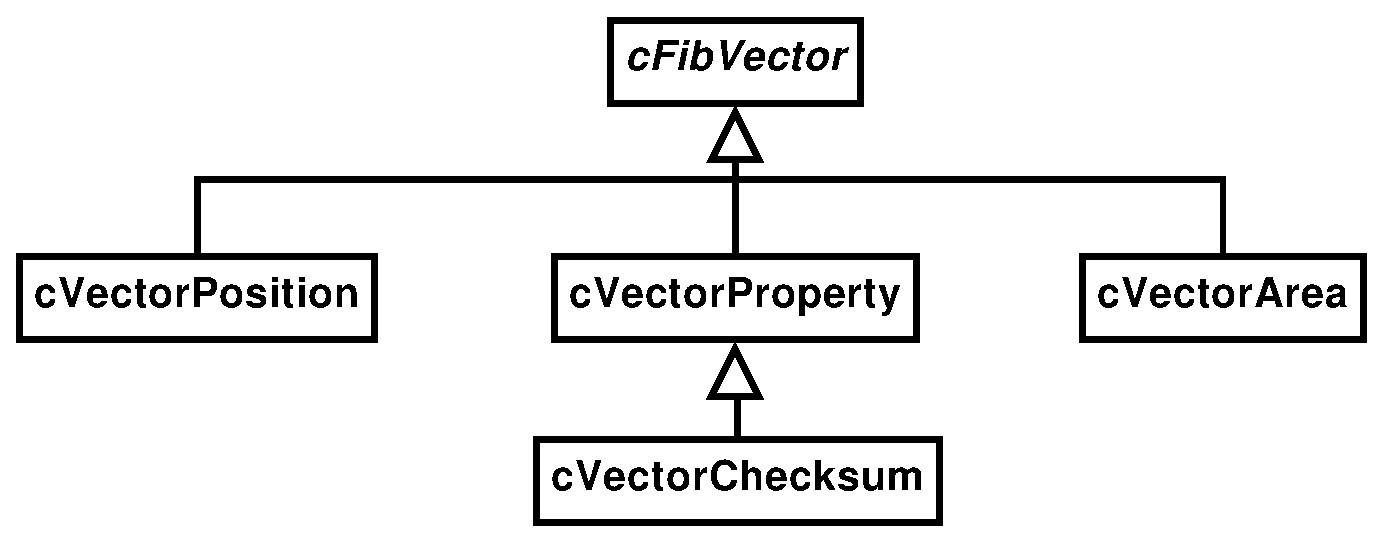
\includegraphics[scale=0.4]{fib_vectors}
\end{center}
\caption{Klassengraph der Fib-Vektoren}
\label{figClassVectors}
\end{figure}


\subsection{Schnittstellenbeschreibung}

\subsubsection{cFibVector}\index{cFibVector}

\textbf{Syntax:} \verb|protected cFibVector(| \\\verb| unsignedIntFib iNumberOfVectorElements=1,| \\\verb| const cFibElement * pDefiningFibElement )|

\bigskip\noindent
Konstruktor eines Vektors, er erzeugt einen Vektors. Da ein allgemeiner Vektor \verb|cFibVector| nicht erzeugt werden kann und soll, ist der Konstruktor au"serhalb der von \verb|cFibVector| abgeleiteten Klassen nicht aufrufbar.

Alle Vektorelemente werden mit 0 initialisiert.

\bigskip\noindent
\textbf{Eingabeparameter:}
\begin{itemize}
 \item \verb|iNumberOfVectorElements|: Die Anzahl der Elemente, welche der Vektor enthalten soll. Standardwert ist 1 .
 \item \verb|pDefiningFibElement|: Ein Zeiger auf das Fib-Element, welches den Vektor enth"alt. Standardwert ist der Nullpointer \verb|NULL|, um anzuzeigen, dass noch kein Fib-Element bekannt ist, welches den Vektor enth"alt.
\end{itemize}

\bigskip\noindent
\textbf{R"uckgabe:} keine


\subsubsection{getElementType}\index{cFibVector!getElementType()}\index{getElementType()}

\textbf{Syntax:} \verb|cTypeElement getElementType() const|

\bigskip\noindent
Diese Methode gibt den Typ des Vektors zur"uck.

\bigskip\noindent
\textbf{Eingabeparameter:} keine

\bigskip\noindent
\textbf{R"uckgabe:} Einen Zeiger auf den Typ des Vektors.


\subsubsection{getNumberOfElements}\index{cFibVector!getNumberOfElements()}\index{getNumberOfElements()}

\textbf{Syntax:} \verb|unsignedIntFib getNumberOfElements() const|

\bigskip\noindent
Diese Methode gibt die Anzahl der Elemente des Vektors zur"uck.

\bigskip\noindent
\textbf{Eingabeparameter:} keine

\bigskip\noindent
\textbf{R"uckgabe:} Die Anzahl der Elemente des Vektors.


\subsubsection{isVariable}\index{cFibVector!isVariable()}\index{isVariable()}

\textbf{Syntax:} \verb|bool isVariable( unsignedIntFib iNumberElement )| \\\verb| const|

\bigskip\noindent
Diese Methode gibt zur"uck, ob das \verb|iNumberElement|'te Element des Vektors eine Variable ist.

\bigskip\noindent
\textbf{Eingabeparameter:}
\begin{itemize}
 \item \verb|iNumberElement|: Die Nummer des Vektorelements, f"ur das zur"uckgegeben werden soll, ob es eine Variable ist.
\end{itemize}

\bigskip\noindent
\textbf{R"uckgabe:} Wenn das \verb|iNumberElement|'te Element des Vektors eine Variable ist, wird \verb|true| (=wahr) zur"uckgegeben, sonst \verb|false| (=falsch).


\subsubsection{getValue}\index{cFibVector!getValue()}\index{getValue()}

\textbf{Syntax:} \verb|doubleFib getValue(| \\\verb| unsignedIntFib iNumberElement ) const|

\bigskip\noindent
Diese Methode gibt den Wert des \verb|iNumberElement|'ten Elements zur"uck.

Dabei wird bei einer Variable ihre Belegung ausgegeben. Ist die Variable nicht belegt, wird der Nullwert des Definitionsbereiches zum Vektorelement zur"uckgegeben.

Der zur"uckgegebene Wert liegt immer im Definitionsbereich des Vektors (auch bez"uglich der anderen Vektorelemente).

\bigskip\noindent
\textbf{Eingabeparameter:}
\begin{itemize}
 \item \verb|iNumberElement|: Die Nummer des Vektorelements, f"ur das der Wert zur"uckgegeben werden soll.
\end{itemize}

\bigskip\noindent
\textbf{R"uckgabe:} Den Wert des \verb|iNumberElement|'ten Elements.


\subsubsection{setValue}\index{cFibVector!setValue()}\index{setValue()}

\textbf{Syntax:} \verb|bool setValue( unsignedIntFib iNumberElement,| \\\verb| doubleFib dValue )|

\bigskip\noindent
Diese Methode setzt das \verb|iNumberElement|'ten Vektorelement auf den Wert \verb|dValue|.

Der Wert \verb|dValue| muss im Definitionsbereich des Vektorelements liegen, um gesetzt werden zu k"onnen. Wenn der Wert \verb|dValue| nicht im Definitionsbereich des Vektorelements liegt, wird das Vektorelement nicht ver"andert und \verb|false| (=falsch) zur"uckgegeben. (Dann sollte eventuell der Definitionsbereich angepasst werden.) Werte die mit der \verb|round|-Methode des zum Vektorelement geh"orenden Definitionsbereich erzeugt wurden (bzw. bei denen die \verb|isElement|-Methode \verb|true| zur"uckgibt), k"onnen immer gesetzt werden.

\bigskip\noindent
\textbf{Eingabeparameter:}
\begin{itemize}
 \item \verb|iNumberElement|: Die Nummer des Vektorelements, f"ur das der Wert \verb|dValue| gesetzt werden soll.
 \item \verb|dValue|: Der Wert \verb|dValue|, welcher gesetzt werden soll.
\end{itemize}

\bigskip\noindent
\textbf{R"uckgabe:} Wenn das \verb|iNumberElement|'te Element des Vektors auf den Wert \verb|dValue| gesetzt wurde, wird \verb|true| (=wahr) zur"uckgegeben, sonst \verb|false| (=falsch).


\subsubsection{getVariable}\index{cFibVector!getVariable()}\index{getVariable()}

\textbf{Syntax:} \verb|cFibVariable *getVariable( unsignedIntFib| \\\verb| iNumberElement )|

\bigskip\noindent
Diese Methode liefert einen Zeiger auf die Variable des \verb|iNumberElement|'ten Vektorelements zur"uck oder \verb|NULL| (Nullpointer), wenn das \verb|iNumber|'te Vektorelement keine Variable ist.

\bigskip\noindent
\textbf{Eingabeparameter:}
\begin{itemize}
 \item \verb|iNumberElement|: Die Nummer des Vektorelements, von dem die Variable zur"uckgegeben werden soll.
\end{itemize}

\bigskip\noindent
\textbf{R"uckgabe:} Einen Zeiger auf die Variable des \verb|iNumberElement|'ten Vektorelements oder \verb|NULL| (Nullpointer), wenn das \verb|iNumberElement|'te Vektorelement keine Variable ist.


\subsubsection{setVariable}\index{cFibVector!setVariable()}\index{setVariable()}

\textbf{Syntax:} \verb|bool setVariable( unsignedIntFib iNumberElement,| \\\verb| cFibVariable *pVariable )|

\bigskip\noindent
Diese Methode setzt das \verb|iNumberElement|'te Vektorelement auf die Variable \verb|pVariable|.

Gibt es kein \verb|iNumberElement|'tes Vektorelement wird \verb|false| (=falsch) zur"uckgegeben.

\bigskip\noindent
\textbf{Eingabeparameter:}
\begin{itemize}
 \item \verb|iNumberElement|: Die Nummer des Vektorelements, f"ur das die Variable \verb|pVariable| gesetzt werden soll.
 \item \verb|pVariable|: Der Zeiger auf die zu setzende Variable.
\end{itemize}

\bigskip\noindent
\textbf{R"uckgabe:} Wenn das \verb|iNumberElement|'te Element des Vektors auf die Variable \verb|pVariable| gesetzt wurde, wird \verb|true| (=wahr) zur"uckgegeben, sonst \verb|false| (=falsch).


\subsubsection{getDomain}\index{cFibVector!getDomain()}\index{getDomain()}

\textbf{Syntax:} \verb|cDomainVectorBasis * getDomain()|

\bigskip\noindent
Diese Methode gibt eine Referenz auf den Definitionsbereich des Vektors zur"uck oder den Nullpointer \verb|NULL|, wenn keine Definitionsbereich f"ur den Vektor definiert ist.
Wenn der Nullpointer \verb|NULL| zur"uckgegeben wurde ist die Standarddomain f"ur den vektor g"ultig.

\bigskip\noindent
\textbf{Eingabeparameter:} keine

\bigskip\noindent
\textbf{R"uckgabe:} Es wird eine Referenz auf den Definitionsbereich des Vektors zur"uckgegeben oder den Nullpointer \verb|NULL|, wenn keine Definitionsbereich f"ur den Vektor definiert ist.


\subsubsection{getDomain}\index{cFibVector!getDomain()}\index{getDomain()}

\textbf{Syntax:} \verb|cDomainSingle *getDomain( unsignedIntFib| \\\verb| iNumberElement )|

\bigskip\noindent
Diese Methode gibt einen Zeiger auf den Definitionsbereich des entsprechenden \verb|iNumberElement|'ten Vektorelements zur"uck oder den Nullpointer \verb|NULL|, wenn keine Definitionsbereich f"ur den Vektor definiert ist.
Wenn der Nullpointer \verb|NULL| zur"uckgegeben wurde ist die Standarddomain f"ur den vektor g"ultig.

\bigskip\noindent
\textbf{Eingabeparameter:}
\begin{itemize}
 \item \verb|iNumberElement|: Die Nummer des Vektorelements, f"ur das der Definitionsbereich zur"uckgegeben werden soll.
\end{itemize}

\bigskip\noindent
\textbf{R"uckgabe:} Es wird einen Zeiger auf den Definitionsbereich des entsprechenden \verb|iNumberElement|'ten Vektorelements oder den Nullpointer \verb|NULL| (wenn keine Definitionsbereich f"ur den Vektor definiert ist) zur"uckgegeben.


\subsubsection{getStandardDomain}\index{cFibVector!getStandardDomain()}\index{getStandardDomai()}

\textbf{Syntax:} \verb|cDomainVectorBasis *getStandardDomain() const|

\bigskip\noindent
Diese Methode gibt eine Referenz auf den Standarddefinitionsbereich des Vektors zur"uck.

\bigskip\noindent
\textbf{Eingabeparameter:} keine

\bigskip\noindent
\textbf{R"uckgabe:} Zur"uckgegeben wird eine Referenz auf den Standarddefinitionsbereich des Vektors.


\subsubsection{getDefiningFibElement}\index{cFibVector!getDefiningFibElement()}\index{getDefiningFibElement()}

\textbf{Syntax:} \verb|cFibElement *getDefiningFibElement() const|

\bigskip\noindent
Diese Methode gibt eine Referenz auf das Fib-Element zur"uck, welches den Vektor definiert bzw. ihn enth"alt.

\bigskip\noindent
\textbf{Eingabeparameter:} keine

\bigskip\noindent
\textbf{R"uckgabe:} Zur"uckgegeben wird eine Referenz auf das Fib-Element, welches den Vektor definiert bzw. enth"alt.


\subsubsection{setDefiningFibElement}\index{cFibVector!setDefiningFibElement()}\index{setDefiningFibElement()}

\textbf{Syntax:} \verb|void setDefiningFibElement(| \\\verb| cFibElement * fibElement=NULL );|

\bigskip\noindent
Diese Methode setzt das Fib-Element, welches den Vektor definiert bzw. enth"alt.

\bigskip\noindent
\textbf{Eingabeparameter:}
\begin{itemize}
 \item \verb|fibElement|: Ein Zeiger auf das Fib-Element, welches den Vektors enth"alt. Standardwert ist der Nullpointer \verb|NULL|, um anzuzeigen das noch kein Fib-Element, welches den Vektors enth"alt, bekannt ist.
\end{itemize}

\bigskip\noindent
\textbf{R"uckgabe:} keine.



\subsection{cVectorPosition}\index{cVectorPosition}\index{cFibVector!cVectorPosition}

\bigskip\noindent
\textbf{Elternklasse:} cFibVector

\bigskip\noindent
\textbf{Standarddefinitionsbereich:} $vector( 2$, $integerB(16)$, $integerB(16) )$

\bigskip\noindent
Dieser Vektor stellt einen Positionsvektor dar. Er kann nur in Punktelementen verwendet werden.


\subsubsection{cVectorPosition}

\textbf{Syntax:} \verb|cVectorPosition(| \\\verb| unsignedIntFib iNumberOfDimensions=2,| \\\verb| cFibElement * pDefiningPointElement=NULL )|

\bigskip\noindent
Der Konstruktor des Positionsvektors, er erstellt einen Positionsvektor.

Initial werden alle Elemente auf den Nullwerte des entsprechenden Definitionsbereichs gesetzt.

\bigskip\noindent
\textbf{Eingabeparameter:}
\begin{itemize}
 \item \verb|iNumberOfDimensions|: Die Anzahl der Dimensionen bzw. Elemente, welche der Positionsvektor enthalten soll. Standardwert ist $2$ .
 \item \verb|pDefiningPointElement|: Ein Zeiger auf das Fib-Element, welches den Vektor enth"alt. Standardwert ist der Nullpointer \verb|NULL|, um anzuzeigen, dass noch kein Fib-Element bekannt ist, welches den Vektor enth"alt.
\end{itemize}

\bigskip\noindent
\textbf{R"uckgabe:} keine


\subsection{cVectorProperty}\index{cFibVector!cVectorProperty}

\bigskip\noindent
\textbf{Elternklasse:} cFibVector

\bigskip\noindent
\textbf{Standarddefinitionsbereich:}  $vector( 0 )$

\bigskip\noindent
Mit diesem Vektor werden die Werte von Eigenschaften gespeichert. Dabei wird der Typ der Eigenschaft, f"ur den der Vektor steht, beim Erzeugen des Objekts festgelegt.


\subsubsection{cVectorProperty}

\textbf{Syntax:} \verb|cVectorProperty( unsignedIntFib uiProperyType,| \\\verb| cFibElement * pDefiningFibElement=NULL )|

\bigskip\noindent
Der Konstruktor des Eigenschaftsvektors, er erstellt einen Eigenschaftsvektor.

Initial werden alle Elemente auf den Nullwerte des entsprechenden Definitionsbereichs gesetzt.

\bigskip\noindent
\textbf{Eingabeparameter:}
\begin{itemize}
 \item \verb|uiProperyType|: Der Typ der Eigenschaft. Dieses ist ein Wert, so wie er in Tabelle \ref{tablePropertyNamen} auf Seite \pageref{tablePropertyNamen} angegeben wird.
 \item \verb|pDefiningFibElement|: Ein Zeiger auf das Fib-Element, welches den Vektor enth"alt. Standardwert ist der Nullpointer \verb|NULL|, um anzuzeigen, dass noch kein Fib-Element bekannt ist, welches den Vektor enth"alt.
\end{itemize}

\bigskip\noindent
\textbf{R"uckgabe:} keine


\subsubsection{cVectorProperty}

\textbf{Syntax:} \verb|cVectorProperty( unsignedIntFib uiProperyType,| \\\verb| unsignedIntFib iNumberOfVectorElements=1,| \\\verb| cFibElement * pDefiningFibElement=NULL )|

\bigskip\noindent
Der Konstruktor des Eigenschaftsvektors, er erstellt einen Eigenschaftsvektor.

Dieser Konstruktor sollte verwendet werden, wenn f"ur die Eigenschaft vom Typ \verb|iProperyType| kein korrekter Standarddefinitionsbereich existiert. (z. B. wie bei den ``Product Properties`` siehe Tabelle \ref{tablePropertyNamen} auf Seite \pageref{tablePropertyNamen})

Initial werden alle Elemente auf den Nullwerte des entsprechenden Definitionsbereichs gesetzt.

\bigskip\noindent
\textbf{Eingabeparameter:}
\begin{itemize}
 \item \verb|uiProperyType|: Der Typ der Eigenschaft. Dieses ist ein Wert, so wie er in Tabelle \ref{tablePropertyNamen} auf Seite \pageref{tablePropertyNamen} angegeben wird.
 \item \verb|iNumberOfVectorElements|: Die Anzahl der Elemente, welche der Vektor enthalten soll. Standardwert ist $1$ .
 \item \verb|pDefiningFibElement|: Ein Zeiger auf das Fib-Element, welches den Vektor enth"alt. Standardwert ist der Nullpointer \verb|NULL|, um anzuzeigen, das noch kein Fib-Element bekannt ist, welches den Vektor enth"alt.
\end{itemize}

\bigskip\noindent
\textbf{R"uckgabe:} keine


\subsubsection{getPropertyType}\index{cVectorProperty!getPropertyType()}\index{getPropertyType()}

\textbf{Syntax:} \verb|unsignedIntFib getPropertyType()|

\bigskip\noindent
Diese Methode gibt den Typ der Eigenschaft zur"uck, so wie er in Tabelle \ref{tablePropertyNamen} auf Seite \pageref{tablePropertyNamen} angegeben wird.

\bigskip\noindent
\textbf{Eingabeparameter:} keine

\bigskip\noindent
\textbf{R"uckgabe:} Den Typ der Eigenschaft.


\subsubsection{cVectorChecksum}\index{cFibVector!cVectorChecksum}

\bigskip\noindent
\textbf{Elternklasse:} cVectorProperty

\bigskip\noindent
\textbf{Standarddefinitionsbereich:}

$vector( 3$, $integerB(4)$,  $integerB(8)$, $integerB(8) )$

\bigskip\noindent
\textbf{Kompatible zu:} Alle Vektoren mit drei Elementen, deren Definitionsbereich aus den nat"urlichen Zahlen kommen.

\bigskip\noindent
Dieser Vektor dient der Typsicherheit des Checksummenvektors im root-Element. Er hat keine eigenen Methoden.


\paragraph{cVectorChecksum}

\ \\\\\noindent
\textbf{Syntax:} \verb|cVectorChecksum(| \\\verb|cFibElement * pDefiningFibElement=NULL )|

\bigskip\noindent
Der Konstruktor des Eigenschaftsvektors f"ur die Checksummeneigenschaft, er erstellt einen Eigenschaftsvektor f"ur die Checksummeneigenschaft.

Initial werden alle Elemente auf den Nullwerte des entsprechenden Definitionsbereichs gesetzt.

%TODO besser gute komprimierungswerte?

\bigskip\noindent
\textbf{Eingabeparameter:}
\begin{itemize}
 \item \verb|pDefiningFibElement|: Ein Zeiger auf das Fib-Element, welches den Vektor enth"alt. Standardwert ist der Nullpointer \verb|NULL|, um anzuzeigen, dass noch kein Fib-Element bekannt ist, welches den Vektor enth"alt.
\end{itemize}


\bigskip\noindent
\textbf{R"uckgabe:} keine


\subsection{cVectorArea}\index{cFibVector!cVectorArea}

\bigskip\noindent
\textbf{Elternklasse:} cFibVector

\bigskip\noindent
\textbf{Standarddefinitionsbereich:} $vector( 2$, $integerB(32)$,  $integerB(32) )$ (Standarddefinitionsbereich von \verb|cTypeArea|)

\bigskip\noindent
Dieser Vektor h"alt die Werte f"ur die untere und obere Grenze eines Unterbereichs (inklusive Grenzen). Beide Werte f"ur die Grenzen sind Ganzzahlen.


\subsubsection{cVectorArea}

\textbf{Syntax 1:} \verb|cVectorArea( longFib lLowerBound,| \\\verb| longFib lUpperBound, | \\\verb|cFibElement * pDefiningFibElement=NULL )|

\noindent
\textbf{Syntax 2:} \verb|cVectorArea( longFib lLowerBound,| \\\verb| cFibVariable & vUpperBound, | \\\verb|cFibElement * pDefiningFibElement=NULL ) )|

\noindent
\textbf{Syntax 3:} \verb|cVectorArea( cFibVariable & vLowerBound,| \\\verb| longFib lUpperBound, | \\\verb|cFibElement * pDefiningFibElement=NULL ) )|

\noindent
\textbf{Syntax 4:} \verb|cVectorArea( cFibVariable & vLowerBound,| \\\verb| cFibVariable & vUpperBound, | \\\verb|cFibElement * pDefiningFibElement=NULL ) )|

\bigskip\noindent
Der Konstruktoren des Bereichsvektors, sie erstellen jeweils einen Bereichsvektor.

\bigskip\noindent
\textbf{Eingabeparameter:}
\begin{itemize}
 \item \verb|lLowerBound|: Die unter Grenze des Bereichs, den der Vektor repr"asentiert.
 \item \verb|vLowerBound|: Eine Referenz auf die Variable, welche die unter Grenze des Bereichs bestimmt, den der Vektor repr"asentiert.
 \item \verb|lUpperBound|: Die ober Grenze des Bereichs, den der Vektor repr"asentiert.
 \item \verb|vUpperBound|: Eine Referenz auf die Variable, welche die obere Grenze des Bereichs bestimmt, den der Vektor repr"asentiert.
 \item \verb|pDefiningFibElement|: Ein Zeiger auf das Fib-Element, welches den Vektor enth"alt. Standardwert ist der Nullpointer \verb|NULL|, um anzuzeigen, dass noch kein Fib-Element bekannt ist, welches den Vektor enth"alt.
\end{itemize}

\bigskip\noindent
\textbf{R"uckgabe:} keine


\subsubsection{getLowerBound}\index{cVectorArea!getLowerBound()}\index{getLowerBound()}

\textbf{Syntax:} \verb|longFib getLowerBound() const|

\bigskip\noindent
Diese Methode gibt die untere Grenze des Bereichs zur"uck.

Dabei wird bei einer Variable ihre Belegung ausgegeben. Ist die Variable nicht belegt, wird der Nullwert des Definitionsbereiches zum Bereichstyp (bzw. des Vektorelements) zur"uckgegeben.

\bigskip\noindent
\textbf{Eingabeparameter:} keine

\bigskip\noindent
\textbf{R"uckgabe:} Die untere Grenze des Bereichs.


\subsubsection{getUpperBound}\index{cVectorArea!getUpperBound()}\index{getUpperBound()}

\textbf{Syntax:} \verb|longFib getUpperBound() const|

\bigskip\noindent
Diese Methode gibt die obere Grenze des Bereichs zur"uck.

Dabei wird bei einer Variable ihre Belegung ausgegeben. Ist die Variable nicht belegt, wird der Nullwert des Definitionsbereiches zum Bereichstyp (bzw. des Vektorelements) zur"uckgegeben.

\bigskip\noindent
\textbf{Eingabeparameter:} keine

\bigskip\noindent
\textbf{R"uckgabe:} Die ober Grenze des Bereichs.


\subsubsection{getAreaValues}\index{cVectorArea!getAreaValues()}\index{getAreaValues()}

\textbf{Syntax:} \verb|list<longFib> getAreaValues() const|

\bigskip\noindent
Diese Methode gibt alle Werte die im Bereich liegen zur"uck.

Dies sind alle Ganzzahlen zwischen der oberen und unteren Grenze des Bereichs (inclusive der Grenzen, wenn diese jeweils Ganzzahlen ist).

Dabei wird bei einer Variable als Grenze ihre Belegung ber"ucksichtigt. Ist die Variable nicht belegt, wird der Nullwert des Definitionsbereiches zum Bereichstyps (bzw. des Vektorelements) ber"ucksichtigt.

\bigskip\noindent
\textbf{Eingabeparameter:} keine

\bigskip\noindent
\textbf{R"uckgabe:} Zur"uckgegeben werden alle Werte, die im Bereich liegen.


\subsubsection{setLowerBoundValue}\index{cVectorArea!setLowerBoundValue()}\index{setLowerBoundValue()}

\textbf{Syntax:} \verb|bool setLowerBoundValue( longFib lValue )|

\bigskip\noindent
Diese Methode setzt die untere Grenze des Bereichs auf den Wert \verb|lValue|.

Der Wert \verb|lValue| muss im Definitionsbereich des Vektorelements bzw. des Bereichstyps liegen, um gesetzt werden zu k"onnen. Wenn der Wert \verb|lValue| nicht im Definitionsbereich des Vektorelements liegt, wird das Vektorelement nicht ver"andert und \verb|false| (=falsch) zur"uckgegeben. (Dann sollte eventuell der Definitionsbereich entsprechend angepasst werden.) Werte die mit der \verb|round|-Methode des zum Vektorelement geh"orenden Definitionsbereich erzeugt wurden (bzw. bei denen die \verb|isElement|-Methode \verb|true| zur"uckgibt), k"onnen immer gesetzt werden.

\bigskip\noindent
\textbf{Eingabeparameter:}
\begin{itemize}
 \item \verb|lValue|: Der f"ur die untere Grenze des Bereichs zu setzende Wert.
\end{itemize}

\bigskip\noindent
\textbf{R"uckgabe:} Wenn die untere Grenze des Bereichs auf den Wert \verb|lValue| gesetzt wurde, wird \verb|true| (=wahr) zur"uckgegeben, sonst \verb|false| (=falsch).


\subsubsection{setUpperBoundValue}\index{cVectorArea!setUpperBoundValue()}\index{setUpperBoundValue()}

\textbf{Syntax:} \verb|bool setUpperBoundValue( longFib lValue )|

\bigskip\noindent
Diese Methode setzt die obere Grenze des Bereichs auf den Wert \verb|lValue|.

Der Wert \verb|lValue| muss im Definitionsbereich des Vektorelements bzw. des Bereichstyps liegen, um gesetzt werden zu k"onnen. Wenn der Wert \verb|lValue| nicht im Definitionsbereich des Vektorelements liegt, wird das Vektorelement nicht ver"andert und \verb|false| (=falsch) zur"uckgegeben. (Dann sollte eventuell der Definitionsbereich entsprechend angepasst werden.) Werte die mit der \verb|round|-Methode des zum Vektorelement geh"orenden Definitionsbereich erzeugt wurden (bzw. bei denen die \verb|isElement|-Methode \verb|true| zur"uckgibt), k"onnen immer gesetzt werden.

\bigskip\noindent
\textbf{Eingabeparameter:}
\begin{itemize}
 \item \verb|lValue|: Der f"ur die obere Grenze des Bereichs zu setzende Wert.
\end{itemize}

\bigskip\noindent
\textbf{R"uckgabe:} Wenn die obere Grenze des Bereichs auf den Wert \verb|lValue| gesetzt wurde, wird \verb|true| (=wahr) zur"uckgegeben, sonst \verb|false| (=falsch).


\subsubsection{setLowerBoundVariable}\index{cVectorArea!setLowerBoundVariable()}\index{setLowerBoundVariable()}

\textbf{Syntax:} \verb|bool setLowerBoundVariable( cFibVariable| \\\verb| *pVariable )|

\bigskip\noindent
Diese Methode setzt die untere Grenze des Bereichs auf die Variable \verb|pVariable|.

\bigskip\noindent
\textbf{Eingabeparameter:}
\begin{itemize}
 \item \verb|pVariable|: Der Zeiger auf die zu setzende Variable.
\end{itemize}

\bigskip\noindent
\textbf{R"uckgabe:} Wenn unter Grenze des Bereichs auf die Variable \verb|pVariable| gesetzt wurde, wird \verb|true| (=wahr) zur"uckgegeben, sonst \verb|false| (=falsch).


\subsubsection{setUpperBoundVariable}\index{cVectorArea!setUpperBoundVariable()}\index{setUpperBoundVariable()}

\textbf{Syntax:} \verb|bool setUpperBoundVariable( cFibVariable| \\\verb| *pVariable )|

\bigskip\noindent
Diese Methode setzt die obere Grenze des Bereichs auf die Variable \verb|pVariable|.

\bigskip\noindent
\textbf{Eingabeparameter:}
\begin{itemize}
 \item \verb|pVariable|: Der Zeiger auf f"ur die zu setzende Variable.
\end{itemize}

\bigskip\noindent
\textbf{R"uckgabe:} Wenn obere Grenze des Bereichs auf die Variable \verb|pVariable| gesetzt wurde, wird \verb|true| (=wahr) zur"uckgegeben, sonst \verb|false| (=falsch).


\subsection{cVectorExtObject}\index{cVectorExtObject}\index{cFibVector!cVectorExtObject}

\bigskip\noindent
\textbf{Elternklasse:} cFibVector

\bigskip\noindent
\textbf{Standarddefinitionsbereich:} $vectorOpenEnd( integerB(8) )$ (Standarddefinitionsbereich von \verb|cTypeExtObjectInput|)

\bigskip\noindent
Dieser Vektor stellt einen Satz bzw. Vektor von Zahlen dar. Er kann nur im externen Objekt Element verwendet werden (siehe Abschnitt \ref{secCExtObjectElement} auf Seite \pageref{secCExtObjectElement} und Abschnitt \ref{secExtObjectElement} auf Seite \pageref{secExtObjectElement} ) .


\subsubsection{cVectorExtObject}

\textbf{Syntax:} \verb|cVectorExtObject(| \\\verb| unsignedIntFib iNumberOfElements=0,| \\\verb| cFibElement * pDefiningMatrixElement=NULL )|

\bigskip\noindent
Der Konstruktor des Vektors f"ur das externen Objekt Element.

Initial werden alle Elemente auf den Nullwerte des entsprechenden Definitionsbereichs gesetzt.

\bigskip\noindent
\textbf{Eingabeparameter:}
\begin{itemize}
 \item \verb|iNumberOfDimensions|: Die Anzahl der Elemente, welche der Vektor enthalten soll. Standardwert ist $0$ .
 \item \verb|pDefiningPointElement|: Ein Zeiger auf das Fib-Element, welches den Vektor enth"alt. Standardwert ist der Nullpointer \verb|NULL|, um anzuzeigen, dass noch kein Fib-Element bekannt ist, welches den Vektor enth"alt.
\end{itemize}

\bigskip\noindent
\textbf{R"uckgabe:} keine


\subsection{cVectorExtSubobject}\index{cVectorExtSubobject}\index{cFibVector!cVectorExtSubobject}

\bigskip\noindent
\textbf{Elternklasse:} cFibVector

\bigskip\noindent
\textbf{Standarddefinitionsbereich:} $vector( 0 )$ (Standarddefinitionsbereich von \verb|cTypeExtSubobject|)

\bigskip\noindent
Dieser Vektor stellt einen Satz bzw. Vektor von Zahlen dar. Er kann nur im externen Unterobjekt Element verwendet werden (siehe Abschnitt \ref{secCExtSubobjectElement} auf Seite \pageref{secCExtSubobjectElement} und Abschnitt \ref{secExtSubobjectElement} auf Seite \pageref{secExtSubobjectElement} ) .


\subsubsection{cVectorExtSubobject}

\textbf{Syntax:} \verb|cVectorExtSubobject(| \\\verb| unsignedIntFib iNumberOfElements=0,| \\\verb| cFibElement * pDefiningMatrixElement=NULL )|

\bigskip\noindent
Der Konstruktor des Vektors f"ur das externen Unterobjekt Element.

Initial werden alle Elemente auf den Nullwerte des entsprechenden Definitionsbereichs gesetzt.

\bigskip\noindent
\textbf{Eingabeparameter:}
\begin{itemize}
 \item \verb|iNumberOfDimensions|: Die Anzahl der Elemente, welche der Vektor enthalten soll. Standardwert ist $0$ .
 \item \verb|pDefiningPointElement|: Ein Zeiger auf das Fib-Element, welches den Vektor enth"alt. Standardwert ist der Nullpointer \verb|NULL|, um anzuzeigen, dass noch kein Fib-Element bekannt ist, welches den Vektor enth"alt.
\end{itemize}

\bigskip\noindent
\textbf{R"uckgabe:} keine


\subsection{cVectorFibSet}\index{cVectorFibSet}\index{cFibVector!cVectorFibSet}

\bigskip\noindent
\textbf{Elternklasse:} cFibVector

\bigskip\noindent
\textbf{Standarddefinitionsbereich:} $vectorOpenEnd( 1,$ $integerB(32) )$ (dritter Unterdefinitionsbereich vom Standarddefinitionsbereich von \verb|cTypeFibSet|)

\bigskip\noindent
Dieser Vektor stellt einen Satz bzw. Vektor von Zahlen dar. Er kann nur im set-Element verwendet werden (siehe Abschnitt \ref{secCFibSetElement} auf Seite \pageref{secCFibSetElement} und Abschnitt \ref{secFibSetElement} auf Seite \pageref{secFibSetElement} ) .


\subsubsection{cVectorFibSet}

\textbf{Syntax:} \verb|cVectorFibSet(| \\\verb| unsignedIntFib iNumberOfElements=2,| \\\verb| cFibElement * pDefiningSetElement=NULL )|

\bigskip\noindent
Der Konstruktor des Vektors f"ur das set-Element.

Initial werden alle Elemente auf den Nullwerte des entsprechenden Definitionsbereichs gesetzt.

\bigskip\noindent
\textbf{Eingabeparameter:}
\begin{itemize}
 \item \verb|iNumberOfElements|: Die Anzahl der Elemente, welche der Vektor enthalten soll. Standardwert ist $2$ .
 \item \verb|pDefiningPointElement|: Ein Zeiger auf das Fib-Element, welches den Vektor enth"alt. Standardwert ist der Nullpointer \verb|NULL|, um anzuzeigen, dass noch kein Fib-Element bekannt ist, welches den Vektor enth"alt.
\end{itemize}

\bigskip\noindent
\textbf{R"uckgabe:} keine


\subsection{cVectorFibMatrix}\index{cVectorFibMatrix}\index{cFibVector!cVectorFibMatrix}

\bigskip\noindent
\textbf{Elternklasse:} cFibVector

\bigskip\noindent
\textbf{Standarddefinitionsbereich:} $vectorOpenEnd( 1,$ $integerB(32) )$ (vierter Unterdefinitionsbereich vom Standarddefinitionsbereich von \verb|cTypeFibMatrix|)

\bigskip\noindent
Dieser Vektor stellt einen Satz bzw. Vektor von Zahlen dar. Er kann nur im Matrixelement verwendet werden (siehe Abschnitt \ref{secCFibMatrixElement} auf Seite \pageref{secCFibMatrixElement} und Abschnitt \ref{secFibMatrixElement} auf Seite \pageref{secFibMatrixElement} ) .


\subsubsection{cVectorFibMatrix}

\textbf{Syntax:} \verb|cVectorFibMatrix(| \\\verb| unsignedIntFib iNumberOfElements=2,| \\\verb| cFibElement * pDefiningMatrixElement=NULL )|

\bigskip\noindent
Der Konstruktor des Vektors f"ur das Matrixelement.

Initial werden alle Elemente auf den Nullwerte des entsprechenden Definitionsbereichs gesetzt.

\bigskip\noindent
\textbf{Eingabeparameter:}
\begin{itemize}
 \item \verb|iNumberOfElements|: Die Anzahl der Elemente, welche der Vektor enthalten soll. Standardwert ist $2$ .
 \item \verb|pDefiningPointElement|: Ein Zeiger auf das Fib-Element, welches den Vektor enth"alt. Standardwert ist der Nullpointer \verb|NULL|, um anzuzeigen, dass noch kein Fib-Element bekannt ist, welches den Vektor enth"alt.
\end{itemize}

\bigskip\noindent
\textbf{R"uckgabe:} keine



\section{cFibVariable}\index{cFibVariable}

Die Klasse \verb|cFibVariable| stellt Variablen f"ur Fib-Objekte dar. Jede Variable muss von einem Fib-Element definiert werden. Nur Fib-Elemente k"onnen deshalb Instanzen von \verb|cFibVariable| erzeugen.

Wenn Variablen in einem Fib-Element verwendet werden, sollte die Variable immer "uber dem Fib-Element definiert werden.

Jede Fib-Variable h"alt sich eine Liste mit Fib-Elementen in den die Variable verwendet wird, sowie eine Referenz auf das Fib-Element in dem die Fib-Variable definiert wird.


\subsection{Schnittstellenbeschreibung}


\subsubsection{cFibVariable}\index{cFibVariable}

\textbf{Syntax:} \verb|cFibVariable(| \\\verb| const cFibElement * pDefiningFibElement )|

\bigskip\noindent
Konstruktor einer Variable, er erzeugt eine Variable.

\bigskip\noindent
\textbf{Eingabeparameter:}
\begin{itemize}
 \item \verb|pDefiningFibElement|: Ein Zeiger auf das Fib-Element, das diese Variable definiert.
\end{itemize}

\bigskip\noindent
\textbf{R"uckgabe:} keine


\subsubsection{getValue}\index{cFibVariable!getValue()}\index{getValue()}

\textbf{Syntax:} \verb|doubleFib getValue() const|

\bigskip\noindent
Diese Methode gibt den Wert der Variable zur"uck oder $0$ wenn, der Variablenwert undefiniert ist.

\bigskip\noindent
\textbf{Eingabeparameter:} keine

\bigskip\noindent
\textbf{R"uckgabe:} Der Wert der Variable oder $0$, wenn der Variablenwert undefiniert ist.


\subsubsection{getIntegerValue}\index{cFibVariable!getIntegerValue()}\index{getIntegerValue}

\textbf{Syntax:} \verb|longFib getIntegerValue() const|

\bigskip\noindent
Diese Methode gibt den Wert der Variable als Ganzzahl zur"uck oder $0$ wenn, der Variablenwert undefiniert ist.

Ist der Inhalt der Variable eine Gleitkommazahl oder skalierte Ganzzahl, wird er auf eine Ganzzahl gerundet und ausgegeben.

Dies ist beispielsweise n"utzlich, wenn der Vektor, in dem die Variable verwendet wird, nur Ganzzahlen enthalten darf (wie z. B. bei Unterbereichsvektoren \verb|cVectorArea|).

\bigskip\noindent
\textbf{Eingabeparameter:} keine

\bigskip\noindent
\textbf{R"uckgabe:} Der Wert der Variable als Ganzzahl oder $0$, wenn der Variablenwert undefiniert ist.


\subsubsection{setValue}\index{cFibVariable!setValue()}\index{setValue()}

\textbf{Syntax:} \verb|void setValue( doubleFib dValue )|

\bigskip\noindent
Diese Methode setzt den Wert der Variable auf den "ubergebenen Wert \verb|dValue|.

Diese Methode ist beispielsweise bei Eingabevariablen des obersten root-\-Ele\-men\-ts n"utzlich.

\bigskip\noindent
\textbf{Eingabeparameter:}
\begin{itemize}
 \item \verb|dValue|: Der Wert, auf den die Variable zu setzen ist.
\end{itemize}

\bigskip\noindent
\textbf{R"uckgabe:} keine


\subsubsection{setIntegerValue}\index{cFibVariable!setIntegerValue()}\index{setIntegerValue()}

\textbf{Syntax:} \verb|void setIntegerValue( longFib lValue )|

\bigskip\noindent
Diese Methode setzt den Wert der Variable auf den "ubergebenen Ganzzahlwert \verb|lValue|.

Diese Methode ist beispielsweise bei Eingabevariablen des obersten root-\-Ele\-men\-ts n"utzlich.

Durch Eingabe eines Ganzzahlwertes k"onnte unter anderem die Sprache oder der Untertitel ausgew"ahlt werden. Gleitkommazahlen k"onnten in solchen Situationen zu Rundungsfehlern f"uhren.

\bigskip\noindent
\textbf{Eingabeparameter:}
\begin{itemize}
 \item \verb|lValue|: Der Ganzzahlwert, auf den die Variable zu setzen ist.
\end{itemize}

\bigskip\noindent
\textbf{R"uckgabe:} keine


\subsubsection{getDefiningElement}\index{cFibVariable!getDefiningElement()}\index{getDefiningElement()}

\textbf{Syntax:} \verb|cFibElement * getDefiningElement() const|

\bigskip\noindent
Diese Methode gibt ein Zeiger auf das Fib-Element zur"uck, in dem die Variable definiert wird.

\bigskip\noindent
\textbf{Eingabeparameter:} keine

\bigskip\noindent
\textbf{R"uckgabe:} Ein Zeiger auf das Fib-Element, in dem die Variable definiert wird.


\subsubsection{getNumberOfUsingElements}\index{cFibVariable!getNumberOfUsingElements()}\index{getNumberOfUsingElements()}

\textbf{Syntax:} \verb|unsignedIntFib getNumberOfUsingElements()|

\bigskip\noindent
Diese Methode gibt die Anzahl der Fib-Elemente zur"uck, in denen die Variable benutzt wird.

Wenn dieser Wert beispielsweise 0 ist, kann das Fib-Element, das die Variable definiert, gel"oscht werden.

\bigskip\noindent
\textbf{Eingabeparameter:} keine

\bigskip\noindent
\textbf{R"uckgabe:} Zur"uckgegeben wird die Anzahl der Fib-Element in denen die Variable benutzt wird.


\subsubsection{registerUsingElement}\index{cFibVariable!registerUsingElement()}\index{registerUsingElement()}

\textbf{Syntax:} \verb|protected void registerUsingElement(| \\\verb| cFibElement * usingElement )|

\bigskip\noindent
Diese Methode registriert das Fib-Element \verb|usingElement| als ein Fib-Element, dass die Variable benutzt.

\bigskip\noindent
\textbf{Eingabeparameter:}
\begin{itemize}
 \item \verb|usingElement|: Ein Zeiger auf das Fib-Element, das diese Variable benutzt.
\end{itemize}

\bigskip\noindent
\textbf{R"uckgabe:} keine


\subsubsection{unregisterUsingElement}\index{cFibVariable!unregisterUsingElement()}\index{unregisterUsingElement()}

\textbf{Syntax:} \verb|protected void unregisterUsingElement(| \\\verb| cFibElement * usingElement )|

\bigskip\noindent
Diese Methode deregistriert das Fib-Element \verb|usingElement| als ein Fib-Element, dass die Variable benutzt. Damit wird der Variable angezeigt, dass das Fib-Element \verb|usingElement| die Variable nicht mehr ben"otigt.

\bigskip\noindent
\textbf{Eingabeparameter:}
\begin{itemize}
 \item \verb|usingElement|: Ein Zeiger auf das Fib-Element, das diese Variable nicht mehr benutzt.
\end{itemize}

\bigskip\noindent
\textbf{R"uckgabe:} keine


\subsubsection{getUsingElements}\index{cFibVariable!getUsingElements()}\index{getUsingElements()}

\textbf{Syntax:} \verb|set< cFibElement* > getUsingElements()|

\bigskip\noindent
Diese Methode gibt eine Menge mit den Zeigern auf die Fib-Elemente zur"uck, in denen die Variable benutzt wird.

Dadurch kann die Variable beispielsweise leichter ersetzt werden, als wenn der gesamte Fib-Unterbaum, "uber den die Variable definierenden Fib-Element, nach der Variable durchsucht werden m"usste.

\bigskip\noindent
\textbf{Eingabeparameter:} keine

\bigskip\noindent
\textbf{R"uckgabe:} Zur"uckgegeben wird eine Menge mit den Zeigern auf die Fib-Elemente, in denen die Variable benutzt wird.



\section{Fib-Unterfunktionen cUnderFunction}\index{Funktion!cUnderFunction}\index{cUnderFunction}\index{Funktion}

Die Klasse \verb|cUnderFunction| ist die Basisklasse aller Unterfunktionen. Aus Unterfunktionen werden Funktionen (mit der Struktur von B"aumen) zusammengestellt. (siehe Abschnitt \ref{fibFunction} auf Seite\pageref{fibFunction} )

Die Klasse \verb|cUnderFunction| dient als Basisklasse aller Unterfunktionen. Von der Klasse \verb|cUnderFunction| k"onnen keine Instanzen erzeugt werden.

Bei der Auswertung von Unterfunktionen ist f"ur den erzeugten Wert der Definitionsbereich f"ur Unterfunktionenen nicht relevant. Wenn also beispielsweise der Definitionsbereich f"ur Unterfunktionenen nur Ganzzahlen enth"alt und eine Unterfunktionen zu $1,5$ ausgewertet wird, wird dieser Wert $1,5$ sowohl von anderen Unterfunktionen direkt (ohne Rundung) verwendet werden, als auch die definierte Variable eines Funktionselements den Wert $1,5$ annehemen.
Der Definitionsbereich f"ur Unterfunktionenen kommt nur zur Anwendung, wenn die Unterfunktion einen Wert enth"alt (also wenn die Unterfunktion \verb|cFunctionValue| ist), oder wenn eine Unterfunktion fehlt und desshalb anstatt ihr der Nullwert des Definitionsbereichs eingesetzt werden soll.

In Abbildung \ref{figClassUnderfunctions} ist ein Klassendiagramm der Unterfunktionen zu sehen.

\begin{figure}[htbp]
\begin{center}
  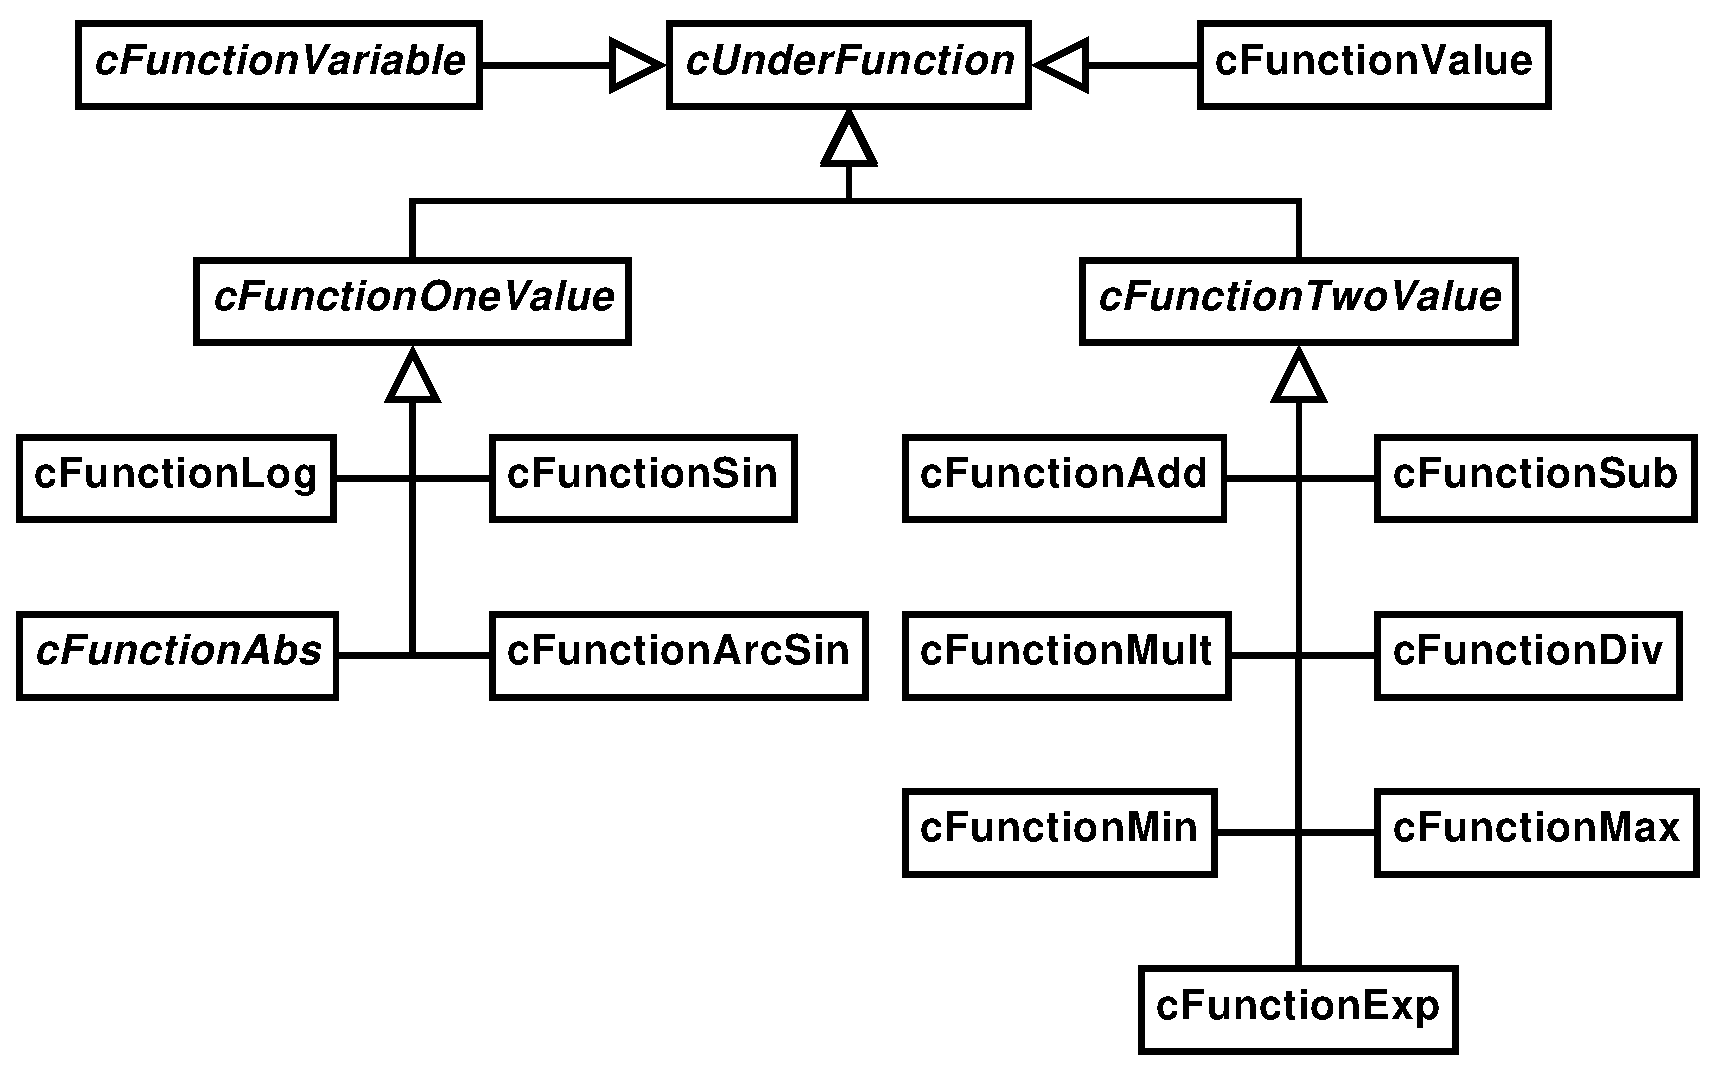
\includegraphics[scale=0.4]{fib_underfunctions}
\end{center}
\caption{Klassengraph der Unterfunktionen}
\label{figClassUnderfunctions}
\end{figure}


\bigskip\noindent
Es gibt drei Arten von Unterfunktionen:
\begin{itemize}
 \item Nullstellige (keine enthaltenden Unterfunktionen)
 \item Einstellige (einen Eingabeparameter bzw. enthaltende Unterfunktionen)
 \item Zweistellige (zwei Eingabeparameter bzw. enthaltende Unterfunktionen)
\end{itemize}

\bigskip\noindent
Die Klassen f"ur die nullstelligen Funktionen sind:
\begin{itemize}
 \item \verb|cFunctionValue|: F"ur einen Wert bzw. eine Konstante.
 \item \verb|cFunctionVariable|: F"ur eine Variable, die "uber dem Fib-Element, welches die Unterfunktion enth"alt, definiert wird.
\end{itemize}

\bigskip\noindent
Die Klassen, welche die einstelligen Funktionen implementieren, werden von der Basisklasse \verb|cFunctionOneValue| abgeleitet.

\bigskip\noindent
Zu diesen einstelligen Funktionen geh"oren:
\begin{itemize}
 \item \verb|cFunctionLog|: Logarithmus
 \item \verb|cFunctionSin|: Sinusfunktion
 \item \verb|cFunctionArcsin|: Arkussinusfunktion
 \item \verb|cFunctionAbs|: Absolutwert
 \item \verb|cFunctionRound|: Runden
\end{itemize}


\bigskip\noindent
Die Klassen, welche die zweistelligen Funktionen implementieren, werden von der Basisklasse \verb|cFunctionTwoValue| abgeleitet.

\bigskip\noindent
Zu diesen zweistelligen Funktionen geh"oren:
\begin{itemize}
 \item \verb|cFunctionAdd|: Addition
 \item \verb|cFunctionSub|: Subtraktion
 \item \verb|cFunctionMult|: Multiplikation
 \item \verb|cFunctionDiv|: Division
 \item \verb|cFunctionExp|: Exponent
 \item \verb|cFunctionMin|: Minimum
 \item \verb|cFunctionMax|: Maximum
 \item \verb|cFunctionIf|: If-Funktion
 \item \verb|cFunctionDelay|: Delay-Funktion
\end{itemize}


\subsection{Schnittstellenbeschreibung}

\subsubsection{getValue}\index{cUnderFunction!getValue()}\index{getValue()}

\textbf{Syntax:} \verb|doubleFib getValue() const|

\bigskip\noindent
Diese Methode berechnet den Wert der Unterfunktion. Dabei werden in der Unterfunktion enthaltenden Unterfunktionen ausgewertet bzw. deren Wert berechnet.

Wenn eine Unterfunktion der Unterfunktion nicht existiert (dies w"are eine ung"ultige Unterfunktion), wird f"ur sie der Nullwert des Definitionsbereichs f"ur Unterfunktionen angenommen.

\bigskip\noindent
\textbf{Eingabeparameter:} keine

\bigskip\noindent
\textbf{R"uckgabe:} Den berechneten Wert der Unterfunktion.


\subsubsection{getType}\index{cUnderFunction!getType()}\index{getType()}

\textbf{Syntax:} \verb|intFib getType() const|

\bigskip\noindent
Diese Methode gibt eine Ganzzahl zur"uck, "uber die der Typ der Unterfunktion bestimmt werden kann. F"ur diese Typen werden auch Konstanten in der Klasse \verb|cUnderFunction| definiert.

\bigskip\noindent
\textbf{M"ogliche Typen sind:}

\noindent
\begin{tabular}{|p{10mm}|p{60mm}|p{40mm}|}\hline
	Typ\-zahl & Unterfunktion & Konstante \\\hline\hline
	00 & \verb|cFunctionValue|: F"ur einen Wert bzw. eine Konstante. & \verb|FUNCTION_VALUE| \\\hline
	01 & \verb|cFunctionVariable|: F"ur eine Variable, die "uber dem Fib-Element, welches die Unterfunktion enth"alt, definiert wird. & \verb|FUNCTION_VARIABLE| \\\hline
	10 & \verb|cFunctionLog|: Logarithmus & \verb|FUNCTION_LOG| \\\hline
	11 & \verb|cFunctionSin|: Sinusfunktion & \verb|FUNCTION_SIN| \\\hline
	12 & \verb|cFunctionAbs|: Absolutwert & \verb|FUNCTION_ABS| \\\hline
	13 & \verb|cFunctionArcsin|: Arkussinusfunktion & \verb|FUNCTION_ARCSIN| \\\hline
	14 & \verb|cFunctionRound|: Rundungsfunktion & \verb|FUNCTION_ROUND| \\\hline
	20 & \verb|cFunctionAdd|: Addition & \verb|FUNCTION_ADD| \\\hline
	21 & \verb|cFunctionSub|: Subtraktion & \verb|FUNCTION_SUB| \\\hline
	22 & \verb|cFunctionMult|: Multiplikation & \verb|FUNCTION_MULT| \\\hline
	23 & \verb|cFunctionDiv|: Division & \verb|FUNCTION_DIV| \\\hline
	24 & \verb|cFunctionExp|: Exponent & \verb|FUNCTION_EXP| \\\hline
	25 & \verb|cFunctionMin|: Minimum & \verb|FUNCTION_MIN| \\\hline
	26 & \verb|cFunctionMax|: Maximum & \verb|FUNCTION_MAX| \\\hline
	30 & \verb|cFunctionIf|: If-Funktion & \verb|FUNCTION_IF| \\\hline
	31 & \verb|cFunctionMod|: Modulo-Funktion & \verb|FUNCTION_MOD| \\\hline
\end{tabular}


\bigskip\noindent
\textbf{Eingabeparameter:} keine

\bigskip\noindent
\textbf{R"uckgabe:} Eine Ganzzahl, "uber die der Typ der Unterfunktion bestimmt werden kann.


\subsubsection{isValid}\index{cUnderFunction!isValid()}\index{isValid()}

\textbf{Syntax:} \verb|bool isValid() const|

\bigskip\noindent
Diese Methode pr"uft, ob die Unterfunktion korrekt ist.

Damit eine Unterfunktion korrekt ist, m"ussen alle direkt oder indirekt enthaltenden Unterfunktionen und Bedingungen (cCondition siehe Abschnitt \ref{secCCondition} auf Seite \pageref{secCCondition}) korrekt sein. Weiterhin m"ussen alle konstanten Unterfunktionen \verb|cFunctionValue| Werte im zugeh"origem Definitionsbereich f"ur Unterfunktionen ``underfunction'' enthalten. Au"serdem m"ussen alle Unterfunktionen f"ur Variablen \verb|cFunctionVariable| ein g"ultige Variable enthalten, welche in einem Fib-Element "uber dem Fib-Element des Funktionsobjekts definiert ist.
Eine korrekte Unterfunktion darf sich nicht selbst enthalten und keine direkt oder indirekt enthaltende Unterfunktion mehr als einmal enthalten. Das hei"st, die direkt oder indirekt enthaltenden Unterfunktionen haben die Struktur eines (zyklenfreien) Baums.

\bigskip\noindent
\textbf{Eingabeparameter:} keine

\bigskip\noindent
\textbf{R"uckgabe:} Wenn die Unterfunktion korrekt ist, wird \verb|true| (=wahr) zur"uckgegeben, sonst \verb|false| (=falsch).


\subsubsection{getDomain}\index{cUnderFunction!getDomain()}\index{getDomain()}

\textbf{Syntax:} \verb|cDomain * getDomain()|

\bigskip\noindent
Diese Methode gibt eine Referenz auf den Definitionsbereich der Unterfunktion zur"uck.

\bigskip\noindent
\textbf{Eingabeparameter:} keine

\bigskip\noindent
\textbf{R"uckgabe:} Eine Referenz auf den Definitionsbereich der Unterfunktion .



\subsection{cFunctionValue}\index{cFunctionValue}\index{Funktion!Konstante}\index{Funktion!Wert}

Die Klasse \verb|cFunctionValue| stellt eine konstante Unterfunktion bzw. einen Wert dar. Sie ist ein Blatt im Unterfunktionsbaum, da sie keine weiteren Unterfunktionen enth"alt. Ihr Wert (R"uckgabe von \verb|getValue()|) ist immer der Wert, der f"ur sie angegeben wurde.


\subsubsection{cFunctionValue}

\textbf{Syntax:} \verb|cFunctionValue( doubleFib dValue )|

\bigskip\noindent
Der Konstruktor der konstante Unterfunktion, er erstellt einen konstante Unterfunktion.

Wenn der "ubergebene Wert au"serhalb des Definitionsbereichs f"ur Unterfunktionen liegt, wird er auf einen Wert im Definitionsbereichs gerundet.

\bigskip\noindent
\textbf{Eingabeparameter:}
\begin{itemize}
 \item \verb|dValue|: Der Wert, den die konstante Unterfunktion zur"uckgeben bzw. repr"asentieren soll.
\end{itemize}

\bigskip\noindent
\textbf{R"uckgabe:} keine


\subsubsection{getValue}\index{cFunctionValue!getValue()}\index{getValue()}

\textbf{Syntax:} \verb|doubleFib getValue() const|

\bigskip\noindent
Diese Methode gibt den Wert der konstanten Unterfunktion zur"uck.

\bigskip\noindent
\textbf{Eingabeparameter:} keine

\bigskip\noindent
\textbf{R"uckgabe:} Der Wert der konstanten Unterfunktion.


\subsubsection{setValue}\index{cFunctionValue!setValue()}\index{setValue()}

\textbf{Syntax:} \verb|bool setValue( doubleFib dValue )|

\bigskip\noindent
Der Methode setzt den Wert der konstanten Unterfunktion auf \verb|dValue|.

Der Wert \verb|dValue| muss im Definitionsbereich f"ur Unterfunktion liegen, um gesetzt werden zu k"onnen. Wenn der Wert \verb|dValue| nicht im Definitionsbereich f"ur Unterfunktion liegt, wird die Unterfunktion nicht ver"andert und \verb|false| (=falsch) zur"uckgegeben. (Dann sollte eventuell der Definitionsbereich angepasst werden.) Werte die mit der \verb|round|-Methode des zum Unterfunktionen geh"orenden Definitionsbereich erzeugt wurden (bzw. bei denen die \verb|isElement|-Methode \verb|true| zur"uckgibt), k"onnen immer gesetzt werden.

\bigskip\noindent
\textbf{Eingabeparameter:}
\begin{itemize}
 \item \verb|dValue|: Der Wert, den die konstante Unterfunktion zur"uckgeben bzw. repr"asentieren soll.
\end{itemize}

\bigskip\noindent
\textbf{R"uckgabe:}  Wenn der Wert der Unterfunktion auf den Wert \verb|dValue| gesetzt wurde, wird \verb|true| (=wahr) zur"uckgegeben, sonst \verb|false| (=falsch).



\subsection{cFunctionVariable}\index{Funktion!cFunctionVariable}\index{cFunctionVariable}\index{Funktion!Variable}

Die Klasse \verb|cFunctionVariable| stellt eine Variable dar. Der Inhalt dieser Variable stellt den Wert (R"uckgabe von \verb|getValue()|) der Unterfunktion dar. Sie ist ein Blatt im Unterfunktionsbaum, da sie keine weiteren Unterfunktionen enth"alt.


\subsubsection{cFunctionVariable}

\textbf{Syntax:} \verb|cFunctionVariable( cFibVariable *fibVariable )|

\bigskip\noindent
Der Konstruktor der Unterfunktion f"ur Variablen, er erstellt einen Unterfunktion f"ur Variablen.

\bigskip\noindent
\textbf{Eingabeparameter:}
\begin{itemize}
 \item \verb|fibVariable|: Einen Zeiger auf die Variable, welche die Unterfunktion repr"asentieren soll. Der Inhalt dieser Variable stellt den Wert der Unterfunktion dar.
\end{itemize}

\bigskip\noindent
\textbf{R"uckgabe:} keine


\subsubsection{getVariable}\index{cFunctionVariable!getVariable()}\index{getVariable()}

\textbf{Syntax:} \verb|cFibVariable * getVariable()|

\bigskip\noindent
Der Methode gibt einen Zeiger auf die Variable, welche die Unterfunktion darstellt, zur"uck.

\bigskip\noindent
\textbf{Eingabeparameter:} keine

\bigskip\noindent
\textbf{R"uckgabe:}  Einen Zeiger auf die Variable, welche die Unterfunktion darstellt.


\subsubsection{setVariable}\index{cFunctionVariable!setVariable()}\index{setVariable()}

\textbf{Syntax:} \verb|bool setVariable( cFibVariable * pFibVariable )|

\bigskip\noindent
Der Methode setzt die Variable, welche die Unterfunktion darstellt, auf die "ubergebene Variable \verb|pFibVariable|.

Diese Operation schl"agt fehl und gibt \verb|false| (=falsch) zur"uck, wenn die Variable \verb|pFibVariable| ein Nullpointer \verb|NULL| ist.

\bigskip\noindent
\textbf{Eingabeparameter:}
\begin{itemize}
 \item \verb|pFibVariable|: Einen Zeiger auf die Variable, welche die Unterfunktion darstellen soll.
\end{itemize}

\bigskip\noindent
\textbf{R"uckgabe:} Wenn die Variable, welche die Unterfunktion darstellt, auf die Variable \verb|pFibVariable| gesetzt wurde, wird \verb|true| (=wahr) zur"uckgegeben, sonst \verb|false| (=falsch).


\subsubsection{getValue}\index{cFunctionVariable!getValue()}\index{getValue()}

\textbf{Syntax:} \verb|doubleFib getValue()|

\bigskip\noindent
Diese Methode gibt den Wert der Variable, welche die Unterfunktion darstellt, zur"uck.

Existiert keine Variable, welche die Unterfunktion darstellt, oder ist die Variable nicht mit einem Wert belegt, wird f"ur sie der Nullwert des Definitionsbereichs f"ur Unterfunktionen zur"uckgegeben.

\bigskip\noindent
\textbf{Eingabeparameter:} keine

\bigskip\noindent
\textbf{R"uckgabe:} Den Wert der Variable, welche die Unterfunktion darstellt.



\subsection{cFunctionOneValue}\index{Funktion!cFunctionOneValue}\index{cFunctionOneValue}\index{Funktion!Einstellig}

Die Klasse \verb|cFunctionOneValue| ist die Basisklasse aller einstelligen Unterfunktionen. Von der Klasse \verb|cFunctionOneValue| k"onnen keine Instanzen erzeugt werden.

Einstellig Unterfunktionen enthalten eine Unterfunktion. Beim Ermitteln des Wertes der Unterfunktion mit \verb|getValue()| wird zuerst der Wert der enthaltenden Unterfunktion ermittelt (mit \verb|getValue()|) . Existiert keine enthaltenden Unterfunktion, wird der Nullwert des Definitionsbereichs f"ur Unterfunktionen als Wert der enthaltenden Unterfunktion angenommen. Bei der Berechnung des Funktionswerts, wird also f"ur fehlende Unterfunktionen der Nullwert eingesetzt.

\bigskip\noindent
Einstellige Unterfunktionen sind:
\begin{itemize}
 \item \verb|cFunctionLog|: Logarithmus
 \item \verb|cFunctionSin|: Sinusfunktion
 \item \verb|cFunctionArcsin|: Arcussinusfunktion
 \item \verb|cFunctionAbs|: Absolutwert
\end{itemize}

Im Folgenden werden zuerst die Methoden f"ur einstellige Unterfunktionen vorgestellt und dann die Klassen der m"oglichen einstellige Unterfunktionen.


\subsubsection{getUnderFunction}\index{cFunctionOneValue!getUnderFunction()}\index{getUnderFunction()}

\textbf{Syntax:} \verb|cUnderFunction * getUnderFunction()|

\bigskip\noindent
Diese Methode gibt einen Zeiger auf die in der einstelligen Unterfunktion enthaltende Unterfunktion zur"uck.

Existiert keine enthaltende Unterfunktion, wird der Nullpointer \verb|NULL| zur"uckgegeben.

\bigskip\noindent
\textbf{Eingabeparameter:} keine

\bigskip\noindent
\textbf{R"uckgabe:} Einen Zeiger auf die in der einstelligen Unterfunktion enthaltende Unterfunktion oder der Nullpointer \verb|NULL| , wenn keine enthaltende Unterfunktion existiert.


\subsubsection{setUnderFunction}\index{cFunctionOneValue!setUnderFunction()}\index{setUnderFunction()}

\textbf{Syntax:} \verb|void setUnderFunction(| \\\verb| cUnderFunction * pUnderFunction,| \\\verb| bool bDeleteOld=true )|

\bigskip\noindent
Diese Methode setzt die in der einstelligen Unterfunktion enthaltende Unterfunktion auf \verb|pUnderFunction|. Dabei wird keine Kopie von \verb|pUnderFunction| erstellt.

\bigskip\noindent
\textbf{Eingabeparameter:}
\begin{itemize}
 \item \verb|pUnderFunction|: Einen Zeiger auf die Unterfunktion, welche die einstelligen Unterfunktion enthalten soll.
 \item \verb|bDeleteOld|: Dieser Parameter gibt an, ob die alte enthaltende Unterfunktion gel"oscht werden soll. Wenn der Wert \verb|true| (=wahr) ist, wird die alte enthaltende Unterfunktion (aus dem Arbeitsspeicher) gel"oscht, sonst, wenn er \verb|false| (=falsch) ist, nicht. Standardwert ist \verb|true|, um die alte enthaltende Unterfunktion zu l"oschen.
\end{itemize}

\bigskip\noindent
\textbf{R"uckgabe:} keine


\subsubsection{cFunctionLog f"ur Logarithmus}\index{Funktion!cFunctionLog}\index{cFunctionLog}\index{Funktion!Logarithmus}

Die Klasse \verb|cFunctionLog| realisiert den nat"urliche Logarithmus. Der nat"urliche Logarithmus ( $\ln{X}$ ) ist zur Basis $e$ zu bestimmen.

\paragraph{cFunctionLog}

\ \\\\\noindent
\textbf{Syntax:} \verb|cFunctionLog( cUnderFunction * pUnderFunction )|

\bigskip\noindent
Der Konstruktor der Logarithmusunterfunktion, er erstellt eine Logarithmusunterfunktion.

\bigskip\noindent
\textbf{Eingabeparameter:}
\begin{itemize}
 \item \verb|pUnderFunction|: Einen Zeiger auf die Unterfunktion, welche die Logarithmusunterfunktion enthalten soll. Die Unterfunktion \verb|pUnderFunction| wird vor dem Einf"ugen nicht kopiert.
\end{itemize}

\bigskip\noindent
\textbf{R"uckgabe:} keine


\paragraph{getValue}\index{cFunctionLog!getValue()}\index{getValue()}

\ \\\\\noindent
\textbf{Syntax:} \verb|doubleFib getValue() const|

\bigskip\noindent
Diese Methode gibt den nat"urliche Logarithmus des Wertes zur"uck, der durch die enthaltende Unterfunktion (mit \verb|getValue()|) ermittelt wird.

\bigskip\noindent
\textbf{Eingabeparameter:} keine

\bigskip\noindent
\textbf{R"uckgabe:} Den nat"urliche Logarithmus des Wertes, der durch die enthaltende Unterfunktion (mit \verb|getValue()|) ermittelt wird.


\subsubsection{cFunctionSin f"ur Sinusfunktion}\index{Funktion!cFunctionSin}\index{cFunctionSin}\index{Funktion!Sinus}

Die Klasse \verb|cFunctionSin| realisiert die Sinusfunktion. Gerechnet wird dabei mit Bogenma"s.

\paragraph{cFunctionSin}

\ \\\\\noindent
\textbf{Syntax:} \verb|cFunctionSin( cUnderFunction * pUnderFunction )|

\bigskip\noindent
Der Konstruktor der Sinusunterfunktion, er erstellt eine Sinusunterfunktion.

\bigskip\noindent
\textbf{Eingabeparameter:}
\begin{itemize}
 \item \verb|pUnderFunction|: Einen Zeiger auf die Unterfunktion, welche die Sinusunterfunktion enthalten soll. Die Unterfunktion \verb|pUnderFunction| wird vor dem Einf"ugen nicht kopiert.
\end{itemize}

\bigskip\noindent
\textbf{R"uckgabe:} keine


\paragraph{getValue}\index{cFunctionSin!getValue()}\index{getValue()}

\ \\\\\noindent
\textbf{Syntax:} \verb|doubleFib getValue() const|

\bigskip\noindent
Diese Methode gibt den Sinuswert des Wertes zur"uck, der durch die enthaltende Unterfunktion (mit \verb|getValue()|) ermittelt wird. Gerechnet wird dabei mit Bogenma"s.

\bigskip\noindent
\textbf{Eingabeparameter:} keine

\bigskip\noindent
\textbf{R"uckgabe:} Den Sinuswert des Wertes, der durch die enthaltende Unterfunktion (mit \verb|getValue()|) ermittelt wird.


\subsubsection{cFunctionArcsin f"ur Arkussinus}\index{Funktion!cFunctionArcsin}\index{cFunctionArcsin}\index{Funktion!Arkussinus}

Die Klasse \verb|cFunctionArcsin| realisiert die Arkussinusfunktion.

\paragraph{cFunctionArcsin}

\ \\\\\noindent
\textbf{Syntax:} \verb|cFunctionArcsin( cUnderFunction * pUnderFunction )|

\bigskip\noindent
Der Konstruktor der Arkussinusfunktion, er erstellt eine Arkussinusfunktion.

\bigskip\noindent
\textbf{Eingabeparameter:}
\begin{itemize}
 \item \verb|pUnderFunction|: Einen Zeiger auf die Unterfunktion, welche die Arkussinusfunktion enthalten soll. Die Unterfunktion \verb|pUnderFunction| wird vor dem Einf"ugen nicht kopiert.
\end{itemize}

\bigskip\noindent
\textbf{R"uckgabe:} keine


\paragraph{getValue}\index{cFunctionArcsin!getValue()}\index{getValue()}

\ \\\\\noindent
\textbf{Syntax:} \verb|doubleFib getValue() const|

\bigskip\noindent
Diese Methode gibt den Arkussinusfunktion des Wertes zur"uck, der durch die enthaltende Unterfunktion (mit \verb|getValue()|) ermittelt wird. 
Zur"uckgegben wird dabei ein Wert in Bogenma"s.

\bigskip\noindent
\textbf{Eingabeparameter:} keine

\bigskip\noindent
\textbf{R"uckgabe:} Den Arkussinus des Wertes, der durch die enthaltende Unterfunktion (mit \verb|getValue()|) ermittelt wird.


\subsubsection{cFunctionAbs f"ur Absolutwert}\index{Funktion!cFunctionAbs}\index{cFunctionAbs}\index{Funktion!Absolutwert}

Die Klasse \verb|cFunctionAbs| realisiert die Absolutwertfunktion.

\paragraph{cFunctionAbs}

\ \\\\\noindent
\textbf{Syntax:} \verb|cFunctionAbs( cUnderFunction * pUnderFunction )|

\bigskip\noindent
Der Konstruktor der Absolutwertunterfunktion, er erstellt eine Absolutwertunterfunktion.

\bigskip\noindent
\textbf{Eingabeparameter:}
\begin{itemize}
 \item \verb|pUnderFunction|: Einen Zeiger auf die Unterfunktion, welche die Absolutwertunterfunktion enthalten soll. Die Unterfunktion \verb|pUnderFunction| wird vor dem Einf"ugen nicht kopiert.
\end{itemize}

\bigskip\noindent
\textbf{R"uckgabe:} keine


\paragraph{getValue}\index{cFunctionAbs!getValue()}\index{getValue()}

\ \\\\\noindent
\textbf{Syntax:} \verb|doubleFib getValue() const|

\bigskip\noindent
Diese Methode gibt den Absolutwert des Wertes zur"uck, der durch die enthaltende Unterfunktion (mit \verb|getValue()|) ermittelt wird. F"ur $x \geq 0$ ist der Absolutwert $x$, sonst bei $x < 0$ ist der Absolutwert $-x$ .

\bigskip\noindent
\textbf{Eingabeparameter:} keine

\bigskip\noindent
\textbf{R"uckgabe:} Den Absolutwert des Wertes, der durch die enthaltende Unterfunktion (mit \verb|getValue()|) ermittelt wird.



\subsubsection{cFunctionRound f"ur Rundung}\index{Funktion!cFunctionRound}\index{cFunctionRound}\index{Funktion!Runden}

Die Klasse \verb|cFunctionRound| realisiert das Runden von zahlen.

\paragraph{cFunctionRound}

\ \\\\\noindent
\textbf{Syntax:} \verb|cFunctionRound( cUnderFunction * pUnderFunction )|

\bigskip\noindent
Der Konstruktor der Rundungsunterfunktion, er erstellt eine Rundungsunterfunktion.

\bigskip\noindent
\textbf{Eingabeparameter:}
\begin{itemize}
 \item \verb|pUnderFunction|: Einen Zeiger auf die Unterfunktion, welche die Rundungsunterfunktion enthalten soll. Die Unterfunktion \verb|pUnderFunction| wird vor dem Einf"ugen nicht kopiert.
\end{itemize}

\bigskip\noindent
\textbf{R"uckgabe:} keine


\paragraph{getValue}\index{cFunctionRound!getValue()}\index{getValue()}

\ \\\\\noindent
\textbf{Syntax:} \verb|doubleFib getValue() const|

\bigskip\noindent
Diese Methode gibt den gerundeten Wert des Wertes zur"uck, der durch die enthaltende Unterfunktion (mit \verb|getValue()|) ermittelt wird. Beim Runden bleibt die Ziffer der Vorkommastelle unver"andert, wenn die Ziffer der ersten Nachkommastelle 0 bis 4 ist, sonst (bei 5 bis 9) wird die Ziffer der Vorkommastelle bei positiven Zahlen um eins erh"oht und bei negativen Zahlen um eins verringert.

\bigskip\noindent
\textbf{Eingabeparameter:} keine

\bigskip\noindent
\textbf{R"uckgabe:} Den gerundeten Wert des Wertes, der durch die enthaltende Unterfunktion (mit \verb|getValue()|) ermittelt wird.




\subsection{cFunctionTwoValue}\index{Funktion!cFunctionTwoValue}\index{cFunctionTwoValue}\index{Funktion!Zweistellig}

Die Klasse \verb|cFunctionTwoValue| ist die Basisklasse aller zweistelligen Unterfunktionen. Von der Klasse \verb|cFunctionTwoValue| k"onnen keine Instanzen erzeugt werden.

Zweistellig Unterfunktionen enthalten zwei Unterfunktionen. Beim Ermitteln des Wertes der Unterfunktion mit \verb|getValue()| , werden zuerst die Werte der enthaltenden Unterfunktionen ermittelt (mit \verb|getValue()|), wobei der Wert der ersten enthaltenden Unterfunktion zuerst ermittelt wird. Existiert eine enthaltenden Unterfunktion nicht, wird der Nullwert des Definitionsbereichs f"ur Unterfunktionen als Wert dieser enthaltenden Unterfunktion angenommen. Bei der Berechnung des Funktionswerts, wird also f"ur fehlende Unterfunktionen der Nullwert eingesetzt.

\bigskip\noindent
Zweistellige Unterfunktionen sind:
\begin{itemize}
 \item \verb|cFunctionAdd|: Addition
 \item \verb|cFunctionSub|: Subtraktion
 \item \verb|cFunctionMult|: Multiplikation
 \item \verb|cFunctionDiv|: Division
 \item \verb|cFunctionExp|: Exponent
 \item \verb|cFunctionMin|: Minimum
 \item \verb|cFunctionMax|: Maximum
\end{itemize}

Im Folgenden werden zuerst die Methoden f"ur zweistellige Unterfunktionen vorgestellt und dann die Klassen der m"oglichen zweistellige Unterfunktionen.


\subsubsection{getFirstUnderFunction}\index{cFunctionTwoValue!getFirstUnderFunction()}\index{getFirstUnderFunction()}

\textbf{Syntax:} \verb|cUnderFunction * getFirstUnderFunction()|

\bigskip\noindent
Diese Methode gibt einen Zeiger auf die erste, in der zweistelligen Unterfunktion enthaltende, Unterfunktion zur"uck.

Existiert keine erste enthaltende Unterfunktion, wird der Nullpointer \verb|NULL| zur"uckgegeben.

\bigskip\noindent
\textbf{Eingabeparameter:} keine

\bigskip\noindent
\textbf{R"uckgabe:} Einen Zeiger auf die erste in der zweistelligen Unterfunktion enthaltende Unterfunktion oder der Nullpointer \verb|NULL| , wenn keine erste enthaltende Unterfunktion existiert.


\subsubsection{setFirstUnderFunction}\index{cFunctionTwoValue!setFirstUnderFunction()}\index{setFirstUnderFunction()}

\textbf{Syntax:} \verb|void setFirstUnderFunction( const cUnderFunction| \\\verb| &underFunction, bool bDeleteOld=true )|

\bigskip\noindent
Diese Methode setzt die erste, in der zweistelligen Unterfunktion enthaltende, Unterfunktion auf \verb|underFunction|. Dabei wird keine Kopie von der "ubergebenen \verb|underFunction| erstellt.

\bigskip\noindent
\textbf{Eingabeparameter:}
\begin{itemize}
 \item \verb|underFunction|: Eine Referenz auf die Unterfunktion, welche die erste einstelligen Unterfunktion sein soll.
 \item \verb|bDeleteOld|: Dieser Parameter gibt an, ob die erste alte enthaltende Unterfunktion gel"oscht werden soll. Wenn der Wert \verb|true| (=wahr) ist, wird die erste alte enthaltende Unterfunktion (aus dem Arbeitsspeicher) gel"oscht, sonst, wenn der Wert \verb|false| (=falsch) ist, nicht. Standardwert ist \verb|true|, um die erste alte enthaltende Unterfunktion zu l"oschen.
\end{itemize}

\bigskip\noindent
\textbf{R"uckgabe:} keine


\subsubsection{getSecondUnderFunction}\index{cFunctionTwoValue!getSecondUnderFunction()}\index{getSecondUnderFunction()}

\textbf{Syntax:} \verb|cUnderFunction * getSecondUnderFunction()|

\bigskip\noindent
Diese Methode gibt einen Zeiger auf die zweite in der zweistelligen Unterfunktion enthaltende Unterfunktion zur"uck.

Existiert keine zweite enthaltende Unterfunktion, wird der Nullpointer \verb|NULL| zur"uckgegeben.

\bigskip\noindent
\textbf{Eingabeparameter:} keine

\bigskip\noindent
\textbf{R"uckgabe:} Einen Zeiger auf die zweite in der zweistelligen Unterfunktion enthaltende Unterfunktion oder der Nullpointer \verb|NULL| , wenn keine zweite enthaltende Unterfunktion existiert.


\subsubsection{setSecondUnderFunction}\index{cFunctionTwoValue!setSecondUnderFunction()}\index{setSecondUnderFunction()}

\textbf{Syntax:} \verb|void setSecondUnderFunction( const cUnderFunction| \\\verb| &underFunction, bool bDeleteOld=true )|

\bigskip\noindent
Diese Methode setzt die zweite, in der zweistelligen Unterfunktion enthaltende, Unterfunktion auf \verb|underFunction|. Dabei wird keine Kopie von der "ubergebenen \verb|underFunction| erstellt.

\bigskip\noindent
\textbf{Eingabeparameter:}
\begin{itemize}
 \item \verb|underFunction|: Eine Referenz auf die Unterfunktion, welche die zweite einstelligen Unterfunktion sein soll.
 \item \verb|bDeleteOld|: Dieser Parameter gibt an, ob die alte zweite enthaltende Unterfunktion gel"oscht werden soll. Wenn der Wert \verb|true| (=wahr) ist wird die zweite alte enthaltende Unterfunktion (aus dem Arbeitsspeicher) gel"oscht, sonst, wenn der Wert \verb|false| (=falsch) ist, nicht. Standardwert ist \verb|true|, um die zweite alte enthaltende Unterfunktion zu l"oschen.
\end{itemize}

\bigskip\noindent
\textbf{R"uckgabe:} keine


\subsubsection{cFunctionAdd f"ur Addition}\index{Funktion!cFunctionAdd}\index{cFunctionAdd}\index{Funktion!Addition}

Die Klasse \verb|cFunctionAdd| realisiert die Addition zweier Zahlen bzw. Unterfunktionswerte.

\paragraph{cFunctionAdd}

\ \\\\\noindent
\textbf{Syntax:} \verb|cFunctionAdd(| \\\verb| cUnderFunction * pFirstUnderFunction,| \\\verb| cUnderFunction * pSecondUnderFunction )|

\bigskip\noindent
Der Konstruktor der Additionsunterfunktion, er erstellt eine Additionsunterfunktion. Dabei wird keine Kopie von den Objekten \verb|pFirstUnderFunction| oder \verb|pSecondUnderFunction| erstellt.

\bigskip\noindent
\textbf{Eingabeparameter:}
\begin{itemize}
 \item \verb|pFirstUnderFunction|:  Einen Zeiger auf die erste Unterfunktion, welche die Additionsunterfunktion enthalten soll. Die "ubergebene Unterfunktion \verb|pFirstUnderFunction| wird vor dem Einf"ugen nicht kopiert.
 \item \verb|pSecondUnderFunction|: Einen Zeiger auf die zweite Unterfunktion, welche die Additionsunterfunktion enthalten soll. Die "ubergebene Unterfunktion \verb|pSecondUnderFunction| wird vor dem Einf"ugen nicht kopiert.
\end{itemize}

\bigskip\noindent
\textbf{R"uckgabe:} keine


\paragraph{getValue}\index{cFunctionAdd!getValue()}\index{getValue()}

\ \\\\\noindent
\textbf{Syntax:} \verb|doubleFib getValue() const|

\bigskip\noindent
Diese Methode gibt die Summe der Werte der enthaltenden Unterfunktionen (mit \verb|getValue()| dieser ermittelt) zur"uck.

\bigskip\noindent
\textbf{Eingabeparameter:} keine

\bigskip\noindent
\textbf{R"uckgabe:} Die Summe der Werte der enthaltenden Unterfunktionen.


\subsubsection{cFunctionSub f"ur Subtraktion}\index{Funktion!cFunctionSub}\index{cFunctionSub}\index{Funktion!Subtraktion}

Die Klasse \verb|cFunctionSub| realisiert die Subtraktion zweier Zahlen bzw. Unterfunktionswerte. Wobei der Wert der zweiten Unterfunktion von dem der ersten abgezogen wird.

\paragraph{cFunctionSub}

\ \\\\\noindent
\textbf{Syntax:} \verb|cFunctionSub(| \\\verb| cUnderFunction * pFirstUnderFunction,| \\\verb| cUnderFunction * pSecondUnderFunction )|

\bigskip\noindent
Der Konstruktor der Subtraktionsunterfunktion, er erstellt eine Subtraktionsunterfunktion. Dabei wird keine Kopie von den Objekten \verb|pFirstUnderFunction| oder \verb|pSecondUnderFunction| erstellt.

\bigskip\noindent
\textbf{Eingabeparameter:}
\begin{itemize}
 \item \verb|pFirstUnderFunction|: Einen Zeiger auf die erste Unterfunktion, welche die Subtraktionsunterfunktion enthalten soll. Die "ubergebene Unterfunktion \verb|pFirstUnderFunction| wird vor dem Einf"ugen nicht kopiert.
 \item \verb|pSecondUnderFunction|: Einen Zeiger auf die zweite Unterfunktion, welche die Subtraktionsunterfunktion enthalten soll. Die "ubergebene Unterfunktion \verb|pSecondUnderFunction| wird vor dem Einf"ugen nicht kopiert.
\end{itemize}

\bigskip\noindent
\textbf{R"uckgabe:} keine


\paragraph{getValue}\index{cFunctionSub!getValue()}\index{getValue()}

\ \\\\\noindent
\textbf{Syntax:} \verb|doubleFib getValue()|

\bigskip\noindent
Diese Methode gibt die Differenz der Werte der enthaltenden Unterfunktionen (mit \verb|getValue()| dieser ermittelt) zur"uck.

\bigskip\noindent
\textbf{Eingabeparameter:} keine

\bigskip\noindent
\textbf{R"uckgabe:} Die Differenz der Werte der enthaltenden Unterfunktionen.


\subsubsection{cFunctionMult f"ur Multiplikation}\index{Funktion!cFunctionMult}\index{cFunctionMult}\index{Funktion!Multiplikation}

Die Klasse \verb|cFunctionMult| realisiert die Multiplikation zweier Zahlen bzw. Unterfunktionswerte.

\paragraph{cFunctionMult}

\ \\\\\noindent
\textbf{Syntax:} \verb|cFunctionMult(| \\\verb| cUnderFunction * pFirstUnderFunction,| \\\verb| cUnderFunction * pSecondUnderFunction )|

\bigskip\noindent
Der Konstruktor der Multiplikationsunterfunktion, er erstellt eine Multiplikationsunterfunktion. Von diesem Konstruktor wird keine Kopie von den beiden "ubergebenen Objekten \verb|pFirstUnderFunction| oder \verb|pSecondUnderFunction| erstellt.

\bigskip\noindent
\textbf{Eingabeparameter:}
\begin{itemize}
 \item \verb|pFirstUnderFunction|: Einen Zeiger auf die erste Unterfunktion, welche die Multiplikationsunterfunktion enthalten soll. Die "ubergebene Unterfunktion \verb|pFirstUnderFunction| wird vor dem Einf"ugen nicht kopiert.
 \item \verb|pSecondUnderFunction|: Einen Zeiger auf die zweite Unterfunktion, welche die Multiplikationsunterfunktion enthalten soll. Die "ubergebene Unterfunktion \verb|pSecondUnderFunction| wird vor dem Einf"ugen nicht kopiert.
\end{itemize}

\bigskip\noindent
\textbf{R"uckgabe:} keine


\paragraph{getValue}\index{cFunctionMult!getValue()}\index{getValue()}

\ \\\\\noindent
\textbf{Syntax:} \verb|doubleFib getValue() const|

\bigskip\noindent
Diese Methode gibt das Produkt der Werte der enthaltenden Unterfunktionen (mit \verb|getValue()| dieser ermittelt) zur"uck.

\bigskip\noindent
\textbf{Eingabeparameter:} keine

\bigskip\noindent
\textbf{R"uckgabe:} Das Produkt der Werte der enthaltenden Unterfunktionen (diese Werte werden mit \verb|getValue()| der Unterfunktionen ermittelt).


\subsubsection{cFunctionDiv f"ur Division}\index{Funktion!cFunctionDiv}\index{cFunctionDiv}\index{Funktion!Division}

Die Klasse \verb|cFunctionDiv| realisiert die Division zweier Zahlen bzw. Unterfunktionswerte. Wobei der Wert $W_1$ der ersten Unterfunktion durch den Wert $W_2$ der zweiten Unterfunktion dividiert wird ($W_1/W_2$). Die ersten Unterfunktion liefert also den Dividend und die zweite den Divisor des Quotienten.

\paragraph{cFunctionDiv}

\ \\\\\noindent
\textbf{Syntax:} \verb|cFunctionDiv(| \\\verb| cUnderFunction * pFirstUnderFunction,| \\\verb| cUnderFunction * pSecondUnderFunction )|

\bigskip\noindent
Der Konstruktor der Divisionsunterfunktion, er erstellt eine Divisionsunterfunktion. Dabei wird keine Kopie von den Objekten \verb|pFirstUnderFunction| oder \verb|pSecondUnderFunction| erstellt.

\bigskip\noindent
\textbf{Eingabeparameter:}
\begin{itemize}
 \item \verb|pFirstUnderFunction|: Einen Zeiger auf die erste Unterfunktion, welche die Divisionsunterfunktion enthalten soll. Die "ubergebene Unterfunktion \verb|pFirstUnderFunction| wird vor dem Einf"ugen nicht kopiert.
 \item \verb|pSecondUnderFunction|: Einen Zeiger auf die zweite Unterfunktion, welche die Divisionsunterfunktion enthalten soll. Die "ubergebene Unterfunktion \verb|pSecondUnderFunction| wird vor dem Einf"ugen nicht kopiert.
\end{itemize}

\bigskip\noindent
\textbf{R"uckgabe:} keine


\paragraph{getValue}\index{cFunctionDiv!getValue()}\index{getValue()}

\ \\\\\noindent
\textbf{Syntax:} \verb|doubleFib getValue() const|

\bigskip\noindent
Diese Methode gibt den Wert des Quotienten der Werte der enthaltenden Unterfunktionen (mit \verb|getValue()| dieser ermittelt) zur"uck.

\bigskip\noindent
\textbf{Eingabeparameter:} keine

\bigskip\noindent
\textbf{R"uckgabe:} Den Wert des Quotienten der Werte der enthaltenden Unterfunktionen (mit \verb|getValue()| dieser ermittelt).



\subsubsection{cFunctionMod f"ur Modulo}\index{Funktion!cFunctionMod}\index{cFunctionMod}\index{Funktion!Modulo}

Die Klasse \verb|cFunctionMod| realisiert den symmetrischen Modulo Operator zweier Zahlen bzw. Unterfunktionswerte. 
Der symmetrische Modulo Operator gibt den Rest beim ganzzahliger Division von $W_1$ und $W_2$ aus.
( $mod( W_1, W_2 ) = W_1 - W_2 * int(W_1/W_2)$; wobei $int$ das Abschneiden der Nachkommastellen bezeichnet ) Die ersten Unterfunktion liefert also den Dividend und die zweite den Divisor des Quotienten.

\paragraph{cFunctionMod}

\ \\\\\noindent
\textbf{Syntax:} \verb|cFunctionMod(| \\\verb| cUnderFunction * pFirstUnderFunction,| \\\verb| cUnderFunction * pSecondUnderFunction )|

\bigskip\noindent
Der Konstruktor der Modulounterfunktion, er erstellt eine Modulounterfunktion. Dabei wird keine Kopie von den Objekten \verb|pFirstUnderFunction| oder \verb|pSecondUnderFunction| erstellt.

\bigskip\noindent
\textbf{Eingabeparameter:}
\begin{itemize}
 \item \verb|pFirstUnderFunction|: Einen Zeiger auf die erste Unterfunktion, welche die Modulounterfunktion enthalten soll. Die "ubergebene Unterfunktion \verb|pFirstUnderFunction| wird vor dem Einf"ugen nicht kopiert.
 \item \verb|pSecondUnderFunction|: Einen Zeiger auf die zweite Unterfunktion, welche die Modulounterfunktion enthalten soll. Die "ubergebene Unterfunktion \verb|pSecondUnderFunction| wird vor dem Einf"ugen nicht kopiert.
\end{itemize}

\bigskip\noindent
\textbf{R"uckgabe:} keine


\paragraph{getValue}\index{cFunctionMod!getValue()}\index{getValue()}

\ \\\\\noindent
\textbf{Syntax:} \verb|doubleFib getValue() const|

\bigskip\noindent
Diese Methode gibt den Wert der symmetrische Modulo Operator der enthaltenden Unterfunktionen (mit \verb|getValue()| dieser ermittelt) zur"uck.
( $mod( W_1, W_2 ) = W_1 - W_2 * int(W_1/W_2)$; wobei $int$ das Abschneiden der Nachkommastellen bezeichnet )

\bigskip\noindent
\textbf{Eingabeparameter:} keine

\bigskip\noindent
\textbf{R"uckgabe:} Den Wert der symmetrische Modulo Operator der enthaltenden Unterfunktionen (mit \verb|getValue()| dieser ermittelt).




\subsubsection{cFunctionExp f"ur Exponent}\index{Funktion!cFunctionExp}\index{cFunctionExp}\index{Funktion!Exponential}

Die Klasse \verb|cFunctionExp| realisiert die Exponentialfunktion zweier Zahlen bzw. Unterfunktionswerte. Wobei der Wert $W_1$ der ersten Unterfunktion hoch dem Wert $W_2$ der zweiten Unterfunktion genommen wird ($W_1^{W_2}$). Der Wert der ersten Unterfunktion ist also die Basis und der Wert der zweiten Unterfunktion der Exponent der Exponentialfunktion.

\paragraph{cFunctionExp}

\ \\\\\noindent
\textbf{Syntax:} \verb|cFunctionExp(| \\\verb| cUnderFunction * pFirstUnderFunction,| \\\verb| cUnderFunction * pSecondUnderFunction )|

\bigskip\noindent
Der Konstruktor der Exponentialunterfunktion, er erstellt eine Exponentialunterfunktion. Dabei wird keine Kopie von den Objekten  \verb|pFirstUnderFunction| oder \verb|pSecondUnderFunction| erstellt.

\bigskip\noindent
\textbf{Eingabeparameter:}
\begin{itemize}
 \item \verb|pFirstUnderFunction|: Einen Zeiger auf die erste Unterfunktion, welche die Exponentialunterfunktion enthalten soll. Die "ubergebene Unterfunktion \verb|pFirstUnderFunction| wird vor dem Einf"ugen nicht kopiert.
 \item \verb|pSecondUnderFunction|: Einen Zeiger auf die zweite Unterfunktion, welche die Exponentialunterfunktion enthalten soll. Die "ubergebene Unterfunktion \verb|pSecondUnderFunction| wird vor dem Einf"ugen nicht kopiert.
\end{itemize}

\bigskip\noindent
\textbf{R"uckgabe:} keine


\paragraph{getValue}\index{cFunctionExp!getValue()}\index{getValue()}

\ \\\\\noindent
\textbf{Syntax:} \verb|doubleFib getValue() const|

\bigskip\noindent
Diese Methode gibt das Ergebnis des Wertes der ersten enthaltenden Unterfunktionen hoch dem Wert der zweiten enthaltenden Unterfunktionen zur"uck.

\bigskip\noindent
\textbf{Eingabeparameter:} keine

\bigskip\noindent
\textbf{R"uckgabe:} Das Ergebnis des Wertes der ersten enthaltenden Unterfunktionen hoch dem Wert der zweiten enthaltenden Unterfunktionen.


\subsubsection{cFunctionMin f"ur Minimum}\index{Funktion!cFunctionMin}\index{cFunctionMin}\index{Funktion!Minimum}

Die Klasse \verb|cFunctionMin| realisiert das Minimum zweier Zahlen bzw. Unterfunktionswerte. Es wird also der kleinste Wert zur"uckgegeben, der von den enthaltenden Unterfunktionen zur"uckgegeben wurde.

\paragraph{cFunctionMin}

\ \\\\\noindent
\textbf{Syntax:} \verb|cFunctionMin(| \\\verb| cUnderFunction * pFirstUnderFunction,| \\\verb| cUnderFunction * pSecondUnderFunction )|

\bigskip\noindent
Der Konstruktor der Minimumsunterfunktion, er erstellt eine Minimumsunterfunktion. Dabei wird keine Kopie von den Objekten \verb|pFirstUnderFunction| oder \verb|pSecondUnderFunction| erstellt.

\bigskip\noindent
\textbf{Eingabeparameter:}
\begin{itemize}
 \item \verb|pFirstUnderFunction|: Einen Zeiger auf die erste Unterfunktion, welche die Minimumsunterfunktion enthalten soll. Die "ubergebene Unterfunktion \verb|pFirstUnderFunction| wird vor dem Einf"ugen nicht kopiert.
 \item \verb|pSecondUnderFunction|: Einen Zeiger auf die zweite Unterfunktion, welche die Minimumsunterfunktion enthalten soll. Die "ubergebene Unterfunktion \verb|pSecondUnderFunction| wird vor dem Einf"ugen nicht kopiert.
\end{itemize}

\bigskip\noindent
\textbf{R"uckgabe:} keine


\paragraph{getValue}\index{cFunctionMin!getValue()}\index{getValue()}

\ \\\\\noindent
\textbf{Syntax:} \verb|doubleFib getValue() const|

\bigskip\noindent
Diese Methode gibt das Minimum der Werte der enthaltenden Unterfunktionen (mit \verb|getValue()| dieser ermittelt) zur"uck.

\bigskip\noindent
\textbf{Eingabeparameter:} keine

\bigskip\noindent
\textbf{R"uckgabe:} Das Minimum der Werte der enthaltenden Unterfunktionen (diese Werte werden mit \verb|getValue()| der Unterfunktionen ermittelt).


\subsubsection{cFunctionMax f"ur Maximum}\index{Funktion!cFunctionMax}\index{cFunctionMax}\index{Funktion!Maximum}

Die Klasse \verb|cFunctionMax| realisiert das Maximum zweier Zahlen bzw. Unterfunktionswerte. Es wird also der gr"o"ste Wert zur"uckgegeben, der von den enthaltenden Unterfunktionen zur"uckgegeben wurde.

\paragraph{cFunctionMax}

\ \\\\\noindent
\textbf{Syntax:} \verb|cFunctionMax(| \\\verb| cUnderFunction * pFirstUnderFunction,| \\\verb| cUnderFunction * pSecondUnderFunction )|

\bigskip\noindent
Der Konstruktor der Maximumsunterfunktion, er erstellt eine Maximumsunterfunktion. Dabei wird keine Kopie von den Objekten \verb|pFirstUnderFunction| oder \verb|pSecondUnderFunction| erstellt.

\bigskip\noindent
\textbf{Eingabeparameter:}
\begin{itemize}
 \item \verb|pFirstUnderFunction|: Einen Zeiger auf die erste Unterfunktion, welche die Maximumsunterfunktion enthalten soll. Die "ubergebene Unterfunktion \verb|pFirstUnderFunction| wird vor dem Einf"ugen nicht kopiert.
 \item \verb|pSecondUnderFunction|: Einen Zeiger auf die zweite Unterfunktion, welche die Maximumsunterfunktion enthalten soll. Die "ubergebene Unterfunktion \verb|pSecondUnderFunction| wird vor dem Einf"ugen nicht kopiert.
\end{itemize}

\bigskip\noindent
\textbf{R"uckgabe:} keine


\paragraph{getValue}\index{cFunctionMax!getValue()}\index{getValue()}

\ \\\\\noindent
\textbf{Syntax:} \verb|doubleFib getValue() const|

\bigskip\noindent
Diese Methode gibt das Maximum der Werte der enthaltenden Unterfunktionen (mit \verb|getValue()| dieser ermittelt) zur"uck.

\bigskip\noindent
\textbf{Eingabeparameter:} keine

\bigskip\noindent
\textbf{R"uckgabe:} Das Maximum der Werte der enthaltenden Unterfunktionen (diese werden mit \verb|getValue()| ermittelt).


%TODO check


\subsubsection{cFunctionIf f"ur die if-Funktion}\index{Funktion!cFunctionIf}\index{cFunctionIf}\index{Funktion!If}

Die Klasse \verb|cFunctionIf| realisiert die if-Funktion zweier Zahlen bzw. Unterfunktionswerte. Wenn die Bedingung wahr ist, wird der Wert der ersten Unterfunktion zur"uckgegeben, sonst der der zweiten.

\paragraph{cFunctionIf}

\ \\\\\noindent
\textbf{Syntax:} \verb|cFunctionIf(| \\\verb| cCondition * pCondition,| \\\verb| cUnderFunction * pFirstUnderFunction,| \\\verb| cUnderFunction * pSecondUnderFunction )|

\bigskip\noindent
Der Konstruktor der if-Unterfunktion, er erstellt eine if-Unterfunktion.
Dabei wird keine Kopie von den Objekten \verb|pFirstUnderFunction| oder \verb|pSecondUnderFunction| erstellt.

\bigskip\noindent
\textbf{Eingabeparameter:}
\begin{itemize}
 \item \verb|pCondition|: Einen Zeiger auf die Bedingung der if-Unterfunktion. Die "ubergebene Bedingung \verb|pCondition| wird vor dem Einf"ugen nicht kopiert.
 \item \verb|pFirstUnderFunction|: Einen Zeiger auf die erste Unterfunktion, welche die if-Unterfunktion enthalten soll. Die "ubergebene Unterfunktion \verb|pFirstUnderFunction| wird vor dem Einf"ugen nicht kopiert.
 \item \verb|pSecondUnderFunction|: Einen Zeiger auf die zweite Unterfunktion, welche die if-Unterfunktion enthalten soll. Die "ubergebene Unterfunktion \verb|pSecondUnderFunction| wird vor dem Einf"ugen nicht kopiert.
\end{itemize}

\bigskip\noindent
\textbf{R"uckgabe:} keine


\paragraph{getValue}\index{cFunctionIf!getValue()}\index{getValue()}

\ \\\\\noindent
\textbf{Syntax:} \verb|doubleFib getValue() const|

\bigskip\noindent
Wenn die Bedingung wahr ist, wird der Wert der ersten Unterfunktion zur"uckgegeben (mit \verb|getValue()| dieser ermittelt), sonst der der zweiten.

\bigskip\noindent
\textbf{Eingabeparameter:} keine

\bigskip\noindent
\textbf{R"uckgabe:} Zur"uckgegeben wird wenn die Bedingung wahr ist, der Wert der ersten Unterfunktion (mit \verb|getValue()| dieser ermittelt), sonst der der zweiten.


\subsubsection{getCondition}\index{cFunctionIf!getCondition()}\index{getCondition()}

\textbf{Syntax:} \verb|cCondition * getCondition()|

\bigskip\noindent
Diese Methode gibt einen Zeiger auf die Bedingung der If-Unterfunktion zur"uck.

\bigskip\noindent
\textbf{Eingabeparameter:} keine

\bigskip\noindent
\textbf{R"uckgabe:} Den Zeiger auf die Bedingung des If-Unterfunktion.


\subsubsection{setCondition}\index{cFunctionIf!setCondition()}\index{setCondition()}

\textbf{Syntax:} \verb|void setCondition( const cCondition & condition)|

\bigskip\noindent
Diese Methode setzt die Bedingung auf die "ubergebene Bedingung \verb|condition|. Eingesetzt wird eine Kopie der "ubergebenen Bedingung \verb|condition| . Die ersetzte Bedingung wird gel"oscht.

\bigskip\noindent
\textbf{Eingabeparameter:}
\begin{itemize}
 \item \verb|condition|: Die Bedingung, welche die aktuelle Bedingung der If-Unterfunktion ersetzen soll.
\end{itemize}

\bigskip\noindent
\textbf{R"uckgabe:} keine


\subsubsection{cFunctionDelay f"ur die Delayfunktion}\index{Funktion!cFunctionDelay}\index{cFunctionDelay}\index{Funktion!Delay}

Die Klasse \verb|cFunctionDelay| realisiert die Delayfunktion f"ur eine Variable. Bei der Auswertung von Fib-Objekten werden einige Zweige mehrfach durchlaufen (z. B. f"ur jeden Wert eines Bereichselements). Die Delayunterfunktion gibt den Wert zur"uck, den die Variable vor $UF_1$-Aufrufen der Delayunterfunktion eingenommen hat. Der Wert $UF_1$ wird dabei durch die erste Unterfunktion bestimmt.

\paragraph{cFunctionDelay}

\ \\\\\noindent
\textbf{Syntax:} \verb|cFunctionDelay(| \\\verb| cFibVariable * pVariable,| \\\verb| cUnderFunction * pUnderFunctionDelay,| \\\verb| cUnderFunction * pUnderFunctionDefault, unsignedLongFib uiMaxDelay=0 )|

\bigskip\noindent
Der Konstruktor der Delay-Unterfunktion, er erstellt eine Delay-Unterfunktion.
Dabei wird keine Kopie von den Objekten \verb|pUnderFunctionDelay| oder \verb|pUnderFunctionDefault| erstellt.

\bigskip\noindent
\textbf{Eingabeparameter:}
\begin{itemize}
 \item \verb|pVariable|: Einen Zeiger auf die Variable $X$ der Delayunterfunktion.
 \item \verb|pUnderFunctionDelay|: Einen Zeiger auf die erste Unterfunktion $UF_1$, welche die Delayunterfunktion enthalten soll. Die "ubergebene Unterfunktion \verb|pUnderFunctionDelay| wird vor dem Einf"ugen nicht kopiert. Der Wert dieser Unterfunktion gibt an, wieviel Durchl"aufe ($UF_1$) der zur"uckzugebene Variablenwert her sein soll.
 \item \verb|pUnderFunctionDefault|: Einen Zeiger auf die zweite Unterfunktion $UF_2$, welche die Delayunterfunktion enthalten soll. Die "ubergebene Unterfunktion \verb|pUnderFunctionDefault| wird vor dem Einf"ugen nicht kopiert. Der Wert dieser Unterfunktion gibt den Wert an, den die Delayunterfunktion einnehmen soll, wenn keine Variablenbelegung von vor $UF_1$-Aufrufen existiert.
 \item \verb|uiMaxDelay|: Eine Zahl, welche die maximale Anzahl der zu speicherenden Variablenbelegungen von \verb|pVariable| angibt. Wenn 0 (Standardwert) werden alle Variablenbelegungen von \verb|pVariable| gespeichert. Wenn der Wert von \verb|pUnderFunctionDelay| gr"o"ser als \verb|uiMaxDelay| ist wird der Wert von \verb|pUnderFunctionDefault| zur"uckgegeben.
\end{itemize}

\bigskip\noindent
\textbf{R"uckgabe:} keine


\paragraph{getValue}\index{cFunctionDelay!getValue()}\index{getValue()}

\ \\\\\noindent
\textbf{Syntax:} \verb|doubleFib getValue() const|

\bigskip\noindent
Die Delayunterfunktion speichert sich f"ur jeden Aufruf $a$ eines Durchgangs den Wert $W_a$, den die Variable $X$ in diesem Aufruf $a$ annimmt. Beim Aufruf $n$ gibt sie den Wert $W_{n-UF_1}$ zur"uck, den die Variable im Aufruf $n-UF_1$ angenommen hat. Ist $n-UF_1$ kleiner als $1$ oder $UF_1$ gr"o"ser als \verb|uiMaxDelay|, wird der Wert der Unterfunktion $UF_2$ zur"uckgegeben.

\bigskip\noindent
\textbf{Eingabeparameter:} keine

\bigskip\noindent
\textbf{R"uckgabe:} Zur"uckgegeben wird der Wert zur"uck, den die Variable $X$ vor $UF_1$-Aufrufen der Delayunterfunktion eingenommen hat oder, wenn dies nicht m"oglich ist, der Standardwert $UF_2$.


\subsubsection{getVariable}\index{cFunctionDelay!getVariable()}\index{getVariable()}

\textbf{Syntax:} \verb|cFibVariable * getVariable()|

\bigskip\noindent
Diese Methode gibt einen Zeiger auf die Variable der Delayunterfunktion zur"uck.

\bigskip\noindent
\textbf{Eingabeparameter:} keine

\bigskip\noindent
\textbf{R"uckgabe:} Einen Zeiger auf die Variable der Delayunterfunktion.


\subsubsection{setVariable}\index{cFunctionDelay!setVariable()}\index{setVariable()}

\textbf{Syntax:} \verb|void setVariable( cFibVariable * pVariable)|

\bigskip\noindent
Diese Methode setzt die Variable auf die "ubergebene Variable \verb|pVariable|.

\bigskip\noindent
\textbf{Eingabeparameter:}
\begin{itemize}
 \item \verb|pVariable|: Einen Zeiger auf die Variable f"ur die Delayunterfunktion.
\end{itemize}

\bigskip\noindent
\textbf{R"uckgabe:} keine




\section{Die Klasse cCondition f"ur Bedingungen}\index{Bedingungen}\index{cCondition}
\label{secCCondition}

Die Klasse \verb|cCondition| ist die Basisklasse aller Bedingungen. Aus einzelnen Bedingungen werden zusammengesetzte Bedingungen (mit der Struktur von B"aumen) zusammengestellt.

Die Klasse \verb|cCondition| dient als Basisklasse aller Bedingungen. Von der Klasse \verb|cCondition| k"onnen keine Instanzen erzeugt werden.

In Abbildung \ref{figClassConditions} ist das Klassendiagramm der Bedingungen zu sehen.

\begin{figure}[htbp]
\begin{center}
  \includegraphics[scale=0.4]{fib_conditions}
\end{center}
\caption{Klassengraph der Bedingungen}
\label{figClassConditions}
\end{figure}


\bigskip\noindent
Es gibt vier Arten von Bedingungen:
\begin{itemize}
 \item Nullstellige (keine Eingabeparameter bzw. enthaltende Bedingungen)
 \item Einstellige (einen Eingabeparameter bzw. enthaltende Bedingungen)
 \item Zweistellige (zwei Eingabeparameter bzw. enthaltende Bedingungen)
 \item Vergleiche (arbeiten auf zwei Unterfunktionen, welche Werte/ Zahlen bereitstellen)
\end{itemize}

\bigskip\noindent
Die Klassen f"ur die nullstelligen Bedingungen realisieren Wahrheitswerte, diese sind:
\begin{itemize}
 \item \verb|cConditionFalse|: Diese Bedingung ist immer falsch/ Unwahr.
 \item \verb|cConditionTrue|: Diese Bedingung ist immer wahr.
\end{itemize}

\bigskip\noindent
Die Klasse f"ur die einstelligen Bedingung ist \verb|cConditionNot| . Sie realisiert die Negation einer Aussage.

\bigskip\noindent
Die Klassen, welche zweistelligen Bedingung darstellen, werden von der Basisklasse \verb|cConditionTwoValue| abgeleitet.

\bigskip\noindent
Zu diesen zweistelligen Bedingungen geh"oren:
\begin{itemize}
 \item \verb|cConditionOr|: Die ``Oder'' Verkn"upfung zweier Wahrheitswerte.
 \item \verb|cConditionAnd|: Die ``Und'' Verkn"upfung zweier Wahrheitswerte.
 \item \verb|cConditionXor|: Die ``Entweder oder'' Verkn"upfung zweier Wahrheitswerte.
\end{itemize}

\bigskip\noindent
Die Klassen, welche Vergleiche von Werten implementieren, werden von der Basisklasse \verb|cConditionComparison| abgeleitet.

\bigskip\noindent
Zu diesen Vergleichen geh"oren:
\begin{itemize}
 \item \verb|cConditionEqualInteger|: Pr"ufung auf Gleichheit, zweier auf Ganzzahlen gerundeter Werte.
 \item \verb|cConditionLower|: Pr"ufung, ob der erste Wert kleiner als der zweite ist.
 \item \verb|cConditionGreater|: Pr"ufung, ob der erste Wert gr"o"ser als der zweite ist.
\end{itemize}


\subsection{Schnittstellenbeschreibung}

\subsubsection{getValue}\index{cCondition!getValue()}\index{getValue()}

\textbf{Syntax:} \verb|bool getValue() const|

\bigskip\noindent
Diese Methode wertet die Bedingung aus. Dabei werden auch in der Bedingung enthaltenden Bedingung ausgewertet.

Wenn eine enthaltende Bedingung der Bedingung nicht existiert, wird f"ur sie der \verb|false| (=falsch) angenommen.

\bigskip\noindent
\textbf{Eingabeparameter:} keine

\bigskip\noindent
\textbf{R"uckgabe:} Der Wahrheitswert zu dem die Bedingung ausgewertet wurde.


\subsubsection{getType}\index{cCondition!getType()}\index{getType()}

\textbf{Syntax:} \verb|intFib getType() const|

\bigskip\noindent
Diese Methode gibt eine Ganzzahl zur"uck, "uber die der Typ der Bedingung bestimmt werden kann. F"ur diese Typen werden auch Konstanten in der Basisklasse \verb|cCondition| definiert.

\bigskip\noindent
\textbf{M"ogliche Typen sind:}

\noindent
\begin{tabular}{|p{10mm}|p{60mm}|p{40mm}|}\hline
	Typ\-zei\-chen & Bedingung & Konstante \\\hline\hline
	00 & \verb|cConditionFalse|: Diese Bedingung ist immer ist falsch/ Unwahr. & \verb|CONDITION_FALSE| \\\hline
	01 & \verb|cConditionTrue|: Diese Bedingung ist immer ist wahr. & \verb|CONDITION_TRUE| \\\hline
	10 & \verb|cConditionNot|: Diese Bedingung realisiert die Negation einer Aussage. & \verb|CONDITION_NOT| \\\hline
	20 & \verb|cConditionOr|: Die ``Oder'' Verkn"upfung zweier Wahrheitswerte. & \verb|CONDITION_OR| \\\hline
	21 & \verb|cConditionAnd|: Die ``Und'' Verkn"upfung zweier Wahrheitswerte. & \verb|CONDITION_AND| \\\hline
	22 & \verb|cConditionXor|: Die ``Entweder oder'' Verkn"upfung zweier Wahrheitswerte. & \verb|CONDITION_XOR| \\\hline
	30 & \verb|cConditionEqualInteger|: Pr"ufung auf Gleichheit, zweier auf Ganzzahlen gerundeter Werte. & \verb|CONDITION_EQUAL_| \verb|INTEGER| \\\hline
	31 & \verb|cConditionLower|: Pr"ufung, ob der erste Wert kleiner als der zweite ist. & \verb|CONDITION_LOWER| \\\hline
	32 & \verb|cConditionGreater|: Pr"ufung, ob der erste Wert gr"o"ser als der zweite ist. & \verb|CONDITION_GREATER| \\\hline
\end{tabular}

\bigskip\noindent
\textbf{Eingabeparameter:} keine

\bigskip\noindent
\textbf{R"uckgabe:} Eine Ganzzahl, "uber die der Typ der Bedingung bestimmt werden kann.


\subsubsection{isValid}\index{cCondition!isValid()}\index{isValid()}

\textbf{Syntax:} \verb|bool isValid() const|

\bigskip\noindent
Diese Methode pr"uft, ob die Bedingung korrekt ist.

Damit eine Bedingung korrekt ist, m"ussen alle direkt oder indirekt enthaltenden Bedingung korrekt sein.
Die in einer korrekten Bedingung enthaltende Vergleichen (von der Klasse \verb|cConditionComparison| abgeleitet Unterklassen) enthaltenden Elemente sind korrekte Unterfunktionen (dies wird mit der \verb|isValid()|-Methode der Unterfunktionen gepr"uft).
Eine korrekte Bedingung darf sich nicht selbst enthalten und keine direkt oder indirekt enthaltende Bedingung oder Unterfunktionen mehr als einmal enthalten. Das hei"st, die direkt oder indirekt enthaltenden Bedingung und Unterfunktionen haben die Struktur eines (zyklenfreien) Baums.

\bigskip\noindent
\textbf{Eingabeparameter:} keine

\bigskip\noindent
\textbf{R"uckgabe:} Wenn die Bedingung korrekt ist, wird \verb|true| (=wahr) zur"uckgegeben, sonst \verb|false| (=falsch).


\subsection{cConditionFalse}\index{cCondition!cConditionFalse}\index{cConditionFalse}\index{Bedingungen!Falsche}

Die Klasse \verb|cConditionFalse| stellt eine Bedingung dar, die immer falsch ist.

\subsubsection{cConditionFalse}

\textbf{Syntax:} \verb|cConditionFalse()|

\bigskip\noindent
Der Konstruktor der falschen Bedingung, er erstellt einen falschen Bedingung.

\bigskip\noindent
\textbf{Eingabeparameter:} keine

\bigskip\noindent
\textbf{R"uckgabe:} keine


\subsubsection{getValue}\index{cConditionFalse!getValue()}\index{getValue()}

\textbf{Syntax:} \verb|bool getValue() const|

\bigskip\noindent
Diese Methode gibt immer \verb|false| (=falsch) zur"uck.

\bigskip\noindent
\textbf{Eingabeparameter:} keine

\bigskip\noindent
\textbf{R"uckgabe:} Es wird immer \verb|false| (=falsch) zur"uckgegeben.


\subsection{cConditionTrue}\index{cCondition!cConditionTrue}\index{cConditionTrue}\index{Bedingungen!Wahre}

Die Klasse \verb|cConditionTrue| stellt eine Bedingung dar, die immer wahr ist.

\subsubsection{cConditionTrue}

\textbf{Syntax:} \verb|cConditionTrue()|

\bigskip\noindent
Der Konstruktor der wahre Bedingung, er erstellt einen wahre Bedingung.

\bigskip\noindent
\textbf{Eingabeparameter:} keine

\bigskip\noindent
\textbf{R"uckgabe:} keine


\subsubsection{getValue}\index{cConditionTrue!getValue()}\index{getValue()}

\textbf{Syntax:} \verb|bool getValue() const|

\bigskip\noindent
Diese Methode gibt immer \verb|true| (=wahr) zur"uck.

\bigskip\noindent
\textbf{Eingabeparameter:} keine

\bigskip\noindent
\textbf{R"uckgabe:} Es wird immer \verb|true| (=wahr) zur"uckgegeben.



\subsection{cConditionNot}\index{cCondition!cConditionNot}\index{cConditionNot}\index{Bedingungen!Negation}

Die Klasse \verb|cConditionNot| stellt eine Bedingung dar, welche den entgegengesetzten Wahrheitswert hat, wie die enthaltende Bedingung. Ist die enthaltende Bedingung wahr ist die \verb|cConditionNot| Bedingung falsch. Ist die enthaltende Bedingung falsch ist die \verb|cConditionNot| Bedingung wahr.

\subsubsection{cConditionNot}

\bigskip\noindent
\textbf{Syntax:} \verb|cConditionNot( cCondition * pSubCondition )|

\bigskip\noindent
Der Konstruktor der Negationsbedingung, er erstellt eine Negationsbedingung.

Von dem Objekt \verb|pSubCondition| wird dabei keine Kope erstellt.

\bigskip\noindent
\textbf{Eingabeparameter:}
\begin{itemize}
 \item \verb|pSubCondition|: Einen Zeiger auf die Bedingung, welche die Negationsbedingung enthalten soll.
\end{itemize}

\bigskip\noindent
\textbf{R"uckgabe:} keine


\subsubsection{getValue}\index{cConditionNot!getValue()}\index{getValue()}

\textbf{Syntax:} \verb|bool getValue() const|

\bigskip\noindent
Diese Methode gibt den Wahrheitswert zur"uck, der das Gegenteil des Wahrheitswerts der enthaltenden Bedingung (mit \verb|getValue()| dieser ermittelt) ist.

Ist die enthaltende Bedingung \verb|true| (=wahr), ist die \verb|cConditionNot| Bedingung \verb|false| (=falsch). Ist die enthaltende Bedingung \verb|false| (=falsch), ist die \verb|cConditionNot| Bedingung \verb|true| (=wahr).

\bigskip\noindent
\textbf{Eingabeparameter:} keine

\bigskip\noindent
\textbf{R"uckgabe:} Den Wahrheitswert, der das Gegenteil des Wahrheitswerts der enthaltenden Bedingung ist (mit \verb|getValue()| dieser ermittelt).


\subsubsection{getSubCondition}\index{cConditionNot!getSubCondition()}\index{getSubCondition()}

\textbf{Syntax:} \verb|cCondition * getSubCondition()|

\bigskip\noindent
Diese Methode gibt einen Zeiger auf die in der Negationsbedingung enthaltende Bedingung zur"uck.

Existiert keine enthaltende Bedingung, wird der Nullpointer \verb|NULL| zur"uckgegeben.

\bigskip\noindent
\textbf{Eingabeparameter:} keine

\bigskip\noindent
\textbf{R"uckgabe:} Einen Zeiger auf die in der Negationsbedingung enthaltende Bedingung oder der Nullpointer \verb|NULL| , wenn keine enthaltende Bedingung existiert.


\subsubsection{setSubCondition}\index{cConditionNot!setSubCondition()}\index{setSubCondition}

\textbf{Syntax:} \verb|bool setSubCondition( cCondition| \\\verb| * pSubCondition, bool bDeleteOld=true )|

\bigskip\noindent
Diese Methode setzt die in der Negationsbedingung enthaltende Bedingung auf \verb|pSubCondition|. Dabei wird keine Kopie von \verb|pSubCondition| erstellt.

\bigskip\noindent
\textbf{Eingabeparameter:}
\begin{itemize}
 \item \verb|pSubCondition|: Einen Zeiger auf die Bedingung, welche die Negationsbedingung enthalten soll.
 \item \verb|bDeleteOld|: Dieser Parameter gibt an, ob die alte enthaltende Bedingung gel"oscht werden soll. Wenn der Wert \verb|true| (=wahr) ist, wird die alte enthaltende Bedingung (aus dem Arbeitsspeicher) gel"oscht. Standardwert ist \verb|true|, um die alte enthaltende Bedingung zu l"oschen.
\end{itemize}

\bigskip\noindent
\textbf{R"uckgabe:} Wenn die entahltende Bedingung auf \verb|pSubCondition| gesetzt wurde \verb|true| (=wahr), sonst \verb|false| (=falsch)


\subsection{cConditionTwoValue}\index{cCondition!cConditionTwoValue}\index{cConditionTwoValue}\index{Bedingungen!Zweistellige}


Die Klasse \verb|cConditionTwoValue| ist die Basisklasse aller zweistelligen Bedingungen. Von der Klasse \verb|cConditionTwoValue| k"onnen keine Instanzen erzeugt werden.

Zweistellig Bedingungen enthalten zwei Bedingungen. Beim Ermitteln des Wahrheitswerts der Bedingungen mit \verb|getValue()| , werden zuerst die Wahrheitswerts der enthaltenden Bedingungen ermittelt (mit \verb|getValue()|), wobei der Wahrheitswerts der ersten enthaltenden Bedingungen zuerst ermittelt wird. Existiert eine enthaltenden Bedingungen nicht, wird der Wahrheitswert falsch (=\verb|false|) als Wert dieser enthaltenden Bedingungen angenommen. Bei der Berechnung des Wahrheitswerts der Bedingung, wird also f"ur fehlende Bedingungen der Wahrheitswert falsch (=\verb|false|) eingesetzt.

\bigskip\noindent
Zweistellige Bedingungen sind:
\begin{itemize}
 \item \verb|cConditionOr|: Die ``Oder'' Verkn"upfung zweier Wahrheitswerte.
 \item \verb|cConditionAnd|: Die ``Und'' Verkn"upfung zweier Wahrheitswerte.
 \item \verb|cConditionXor|: Die ``Entweder oder'' Verkn"upfung zweier Wahrheitswerte.
\end{itemize}

Im Folgenden werden zuerst die Methoden f"ur zweistellige Bedingungen vorgestellt und dann die Klassen der m"oglichen zweistellige Bedingungen.


\subsubsection{getFirstSubCondition}\index{cConditionTwoValue!getFirstSubCondition()}\index{getFirstSubCondition()}

\textbf{Syntax:} \verb|cCondition * getFirstSubCondition()|

\bigskip\noindent
Diese Methode gibt einen Zeiger auf die erste in der Bedingungen enthaltende Bedingung zur"uck.

Existiert keine erste enthaltende Bedingung, wird der Nullpointer \verb|NULL| zur"uckgegeben.

\bigskip\noindent
\textbf{Eingabeparameter:} keine

\bigskip\noindent
\textbf{R"uckgabe:} Einen Zeiger auf die erste in der Bedingungen enthaltende Bedingung oder der Nullpointer \verb|NULL| , wenn keine erste enthaltende Bedingung existiert.


\subsubsection{setFirstSubCondition}\index{cConditionTwoValue!setFirstSubCondition()}\index{setFirstSubCondition()}

\textbf{Syntax:} \verb|bool setFirstSubCondition(| \\\verb| cCondition * pSubCondition, bool bDeleteOld=true )|

\bigskip\noindent
Diese Methode setzt die erste in der Bedingungen enthaltende Bedingung auf die "ubergebende Unterbedingung \verb|pSubCondition|. Dabei wird keine Kopie von \verb|pSubCondition| erstellt.

\bigskip\noindent
\textbf{Eingabeparameter:}
\begin{itemize}
 \item \verb|pSubCondition|: Einen Zeiger auf die Bedingung, welche die erste Unternbedingungen enthalten soll.
 \item \verb|bDeleteOld|: Dieser Parameter gibt an, ob die alte erste enthaltende Bedingung gel"oscht werden soll. Wenn der Wert \verb|true| (=wahr) ist, wird die erste alte enthaltende Bedingung (aus dem Arbeitsspeicher) gel"oscht, sonst, wenn er \verb|false| (=falsch) ist, nicht. Standardwert ist \verb|true|, um die erste alte enthaltende Bedingung zu l"oschen.
\end{itemize}

\bigskip\noindent
\textbf{R"uckgabe:} Wenn die entahltende erste Bedingung auf \verb|pSubCondition| gesetzt wurde \verb|true| (=wahr), sonst \verb|false| (=falsch)


\subsubsection{getSecondSubCondition}\index{cConditionTwoValue!getSecondSubCondition()}\index{getSecondSubCondition()}

\textbf{Syntax:} \verb|cCondition * getSecondSubCondition()|

\bigskip\noindent
Diese Methode gibt einen Zeiger auf die zweite in der Bedingungen enthaltende Bedingung zur"uck.

Existiert keine zweite enthaltende Bedingung, wird der Nullpointer \verb|NULL| zur"uckgegeben.

\bigskip\noindent
\textbf{Eingabeparameter:} keine

\bigskip\noindent
\textbf{R"uckgabe:} Einen Zeiger auf die zweite in der Bedingungen enthaltende Bedingung oder der Nullpointer \verb|NULL| , wenn keine zweite enthaltende Bedingung existiert.


\subsubsection{setSecondSubCondition}\index{cConditionTwoValue!setSecondSubCondition()}\index{setSecondSubCondition()}

\textbf{Syntax:} \verb|bool setSecondSubCondition(| \\\verb| cCondition * pSubCondition, bool bDeleteOld=true )|

\bigskip\noindent
Diese Methode setzt die zweite in der Bedingungen enthaltende Bedingung auf \verb|pSubCondition|. Dabei wird keine Kopie von \verb|pSubCondition| erstellt.

\bigskip\noindent
\textbf{Eingabeparameter:}
\begin{itemize}
 \item \verb|pSubCondition|: Einen Zeiger auf die Bedingung, welche die zweite Unternbedingungen enthalten soll.
 \item \verb|bDeleteOld|: Dieser Parameter gibt an, ob die alte zweite enthaltende Bedingung gel"oscht werden soll. Wenn der Wert \verb|true| (=wahr) ist, wird die zweite alte enthaltende Bedingung (aus dem Arbeitsspeicher) gel"oscht, sonst, wenn er \verb|false| (=falsch) ist, nicht. Standardwert ist \verb|true|, um die zweite alte enthaltende Bedingung zu l"oschen.
\end{itemize}

\bigskip\noindent
\textbf{R"uckgabe:} Wenn die entahltende zweite Bedingung auf \verb|pSubCondition| gesetzt wurde \verb|true| (=wahr), sonst \verb|false| (=falsch)


\subsubsection{cConditionOr}\index{cCondition!cConditionOr}\index{cConditionOr}\index{Bedingungen!Oder}

Die Klasse \verb|cConditionOr| realisiert die ``Or''-Bedingung zweier Unterbedingungen. Die ``Or''-Bedingung ist wahr (=\verb|true|), wenn mindestens eine der Unterbedingungen wahr (=\verb|true|) ist, sonst ist sie falsch  (=\verb|false|).

\paragraph{cConditionOr}

\ \\\\\noindent
\textbf{Syntax:} \verb|cConditionOr( cCondition * pFirstSubCondition,| \\\verb| cCondition * pSecondSubCondition )|

\bigskip\noindent
Der Konstruktor der ``Or''-Bedingung, er erstellt eine ``Or''-Bedingung. Es wird keine Kopie von \verb|pFirstSubCondition| oder \verb|pSecondSubCondition| erstellt.

\bigskip\noindent
\textbf{Eingabeparameter:}
\begin{itemize}
 \item \verb|pFirstSubCondition|: Einen Zeiger auf die erste Unterbedingung, welche die ``Or''-Bedingung enthalten soll.
 \item \verb|pSecondSubCondition|: Einen Zeiger auf die zweite Unterbedingung, welche die ``Or''-Bedingung enthalten soll.
\end{itemize}

\bigskip\noindent
\textbf{R"uckgabe:} keine


\paragraph{getValue}\index{cConditionOr!getValue()}\index{getValue()}

\ \\\\\noindent
\textbf{Syntax:} \verb|bool getValue() const|

\bigskip\noindent
Diese Methode gibt \verb|true| (=wahr) zur"uck, wenn mindestens einer der Wahrheitswerte der enthaltenden Unterbedingungen (mit \verb|getValue()| dieser ermittelt) \verb|true| (=wahr) ist, sonst gibt sie \verb|false| (=falsch) zur"uck.

\bigskip\noindent
\textbf{Eingabeparameter:} keine

\bigskip\noindent
\textbf{R"uckgabe:} Es wird \verb|true| (=wahr) zur"uckgegeben, wenn mindestens einer der Wahrheitswerte der enthaltenden Unterbedingungen (mit \verb|getValue()| dieser ermittelt) \verb|true| (=wahr) ist, sonst \verb|false| (=falsch).


\subsubsection{cConditionAnd}\index{cCondition!cConditionAnd}\index{cConditionAnd}\index{Bedingungen!Und}

Die Klasse \verb|cConditionAnd| realisiert die ``And''-Bedingung zweier Unterbedingungen. Die ``And''-Bedingung ist wahr (=\verb|true|), wenn beide der Unterbedingungen wahr (=\verb|true|) sind, sonst ist sie falsch  (=\verb|false|).

\paragraph{cConditionAnd}

\ \\\\\noindent
\textbf{Syntax:} \verb|cConditionAnd( cCondition * pFirstSubCondition,| \\\verb| cCondition * pSecondSubCondition )|

\bigskip\noindent
Der Konstruktor der ``And''-Bedingung, er erstellt eine ``And''-Bedingung. Dabei wird keine Kopie von dem Objekt \verb|pFirstSubCondition| oder dem Objekt \verb|pSecondSubCondition| erstellt.

\bigskip\noindent
\textbf{Eingabeparameter:}
\begin{itemize}
 \item \verb|pFirstSubCondition|: Einen Zeiger auf die erste Unterbedingung, welche die ``And''-Bedingung enthalten soll.
 \item \verb|pSecondSubCondition|: Einen Zeiger auf die zweite Unterbedingung, welche die ``And''-Bedingung enthalten soll.
\end{itemize}

\bigskip\noindent
\textbf{R"uckgabe:} keine


\paragraph{getValue}\index{cConditionAnd!getValue()}\index{getValue()}

\ \\\\\noindent
\textbf{Syntax:} \verb|bool getValue() const|

\bigskip\noindent
Diese Methode gibt \verb|true| (=wahr) zur"uck, wenn beide der Wahrheitswerte der enthaltenden Unterbedingungen (mit \verb|getValue()| dieser ermittelt) \verb|true| (=wahr) sind, sonst gibt sie \verb|false| (=falsch) zur"uck.

\bigskip\noindent
\textbf{Eingabeparameter:} keine

\bigskip\noindent
\textbf{R"uckgabe:} Es wird \verb|true| (=wahr) zur"uckgegeben, wenn beide der Wahrheitswerte der enthaltenden Unterbedingungen (mit \verb|getValue()| dieser ermittelt) \verb|true| (=wahr) sind, sonst \verb|false| (=falsch).


\subsubsection{cConditionXor}\index{cCondition!cConditionXor}\index{cConditionXor}\index{Bedingungen!Xor}

Die Klasse \verb|cConditionXor| realisiert die ``Xor''-Bedingung zweier Unterbedingungen. Die ``Xor''-Bedingung ist wahr (=\verb|true|), wenn genau eine der Unterbedingungen wahr (=\verb|true|) ist, sonst ist sie falsch  (=\verb|false|).

\paragraph{cConditionXor}

\ \\\\\noindent
\textbf{Syntax:} \verb|cConditionXor( cCondition * pFirstSubCondition,| \\\verb| cCondition * pSecondSubCondition )|

\bigskip\noindent
Der Konstruktor der ``Xor''-Bedingung, er erstellt eine ``Xor''-Bedingung. Dabei wird keine Kopie von dem Objekt \verb|pFirstSubCondition| oder dem Objekt \verb|pSecondSubCondition| erstellt.

\bigskip\noindent
\textbf{Eingabeparameter:}
\begin{itemize}
 \item \verb|pFirstSubCondition|: Einen Zeiger auf die erste Unterbedingung, welche die ``Xor''-Bedingung enthalten soll.
 \item \verb|pSecondSubCondition|: Einen Zeiger auf die zweite Unterbedingung, welche die ``Xor''-Bedingung enthalten soll.
\end{itemize}

\bigskip\noindent
\textbf{R"uckgabe:} keine


\paragraph{getValue}\index{cConditionXor!getValue()}\index{getValue()}

\ \\\\\noindent
\textbf{Syntax:} \verb|bool getValue() const|

\bigskip\noindent
Diese Methode gibt \verb|true| (=wahr) zur"uck, wenn genau einer der Wahrheitswerte der enthaltenden Unterbedingungen (mit \verb|getValue()| dieser ermittelt) \verb|true| (=wahr) ist, sonst gibt sie \verb|false| (=falsch) zur"uck.

\bigskip\noindent
\textbf{Eingabeparameter:} keine

\bigskip\noindent
\textbf{R"uckgabe:} Es wird \verb|true| (=wahr) zur"uckgegeben, wenn genau einer der Wahrheitswerte der enthaltenden Unterbedingungen (mit \verb|getValue()| dieser ermittelt) \verb|true| (=wahr) ist, sonst \verb|false| (=falsch).



\subsection{cConditionComparison}\index{cCondition!cConditionComparison}\index{cConditionComparison}\index{Bedingungen!Vergleiche}


Die Klasse \verb|cConditionComparison| ist die Basisklasse aller Vergleiche. Von der Klasse \verb|cConditionComparison| k"onnen keine Instanzen erzeugt werden.

Vergleiche geschehen immer auf zwei Unterfunktionen.

Vergleiche enthalten zwei Unterfunktionen. Beim Ermitteln des Wahrheitswerts des Vergleichs mit \verb|getValue()| , werden zuerst die Werte der enthaltenden Unterfunktionen ermittelt (mit \verb|getValue()|), wobei der Wert der ersten enthaltenden Unterfunktion zuerst ermittelt wird. Existiert eine enthaltenden Unterfunktion nicht, wird der Nullwert des Definitionsbereichs f"ur Unterfunktionen als Wert dieser Unterfunktion angenommen. Bei der Berechnung des Wahrheitswerts, wird also f"ur fehlende Unterfunktionen der Nullwert eingesetzt.

\bigskip\noindent
Vergleiche sind:
\begin{itemize}
 \item \verb|cConditionEqualInteger|: Pr"ufung auf Gleichheit, zweier auf Ganzzahlen gerundeter Werte.
 \item \verb|cConditionLower|: Pr"ufung, ob der erste Wert kleiner als der zweite ist.
 \item \verb|cConditionGreater|: Pr"ufung, ob der erste Wert gr"o"ser als der zweite ist.
\end{itemize}

Im Folgenden werden zuerst die Methoden f"ur Vergleiche vorgestellt und dann die Klassen der m"oglichen Vergleiche.



\subsubsection{getFirstUnderFunction}\index{cConditionComparison!getFirstUnderFunction()}\index{getFirstUnderFunction()}

\textbf{Syntax:} \verb|cUnderFunction * getFirstUnderFunction()|

\bigskip\noindent
Diese Methode gibt einen Zeiger auf die erste in dem Vergleich enthaltende Unterfunktion zur"uck.

Existiert keine erste enthaltende Unterfunktion, wird der Nullpointer \verb|NULL| zur"uckgegeben.

\bigskip\noindent
\textbf{Eingabeparameter:} keine

\bigskip\noindent
\textbf{R"uckgabe:} Einen Zeiger auf die erste in dem Vergleich enthaltende Unterfunktion oder der Nullpointer \verb|NULL| , wenn keine erste enthaltende Unterfunktion existiert.


\subsubsection{setFirstUnderFunction}\index{cConditionComparison!setFirstUnderFunction()}\index{setFirstUnderFunction()}

\textbf{Syntax:} \verb|void setFirstUnderFunction(| \\\verb| cUnderFunction *pUnderFunction, bool bDeleteOld=true )|

\bigskip\noindent
Diese Methode setzt die erste in dem Vergleich enthaltende Unterfunktion auf \verb|pUnderFunction|. Dabei wird keine Kopie von \verb|pUnderFunction| erstellt.

\bigskip\noindent
\textbf{Eingabeparameter:}
\begin{itemize}
 \item \verb|pUnderFunction|: Einen Zeiger auf die Unterfunktion, welche als die erste Unterfunktion enthalten sein soll.
 \item \verb|bDeleteOld|: Dieser Parameter gibt an, ob die erste alte enthaltende Unterfunktion gel"oscht werden soll. Wenn der Wert \verb|true| (=wahr) ist, wird die erste alte enthaltende Unterfunktion (aus dem Arbeitsspeicher) gel"oscht, sonst, wenn der Wert \verb|false| (=falsch) ist, nicht. Standardwert ist \verb|true|, um die erste alte enthaltende Unterfunktion zu l"oschen.
\end{itemize}

\bigskip\noindent
\textbf{R"uckgabe:} keine


\subsubsection{getSecondUnderFunction}\index{cConditionComparison!getSecondUnderFunction()}\index{getSecondUnderFunction()}

\textbf{Syntax:} \verb|cUnderFunction * getSecondUnderFunction()|

\bigskip\noindent
Diese Methode gibt einen Zeiger auf die zweite in dem Vergleich enthaltende Unterfunktion zur"uck.

Existiert keine zweite enthaltende Unterfunktion, wird der Nullpointer \verb|NULL| zur"uckgegeben.

\bigskip\noindent
\textbf{Eingabeparameter:} keine

\bigskip\noindent
\textbf{R"uckgabe:} Einen Zeiger auf die zweite in dem Vergleich enthaltende Unterfunktion oder der Nullpointer \verb|NULL| , wenn keine zweite enthaltende Unterfunktion existiert.


\subsubsection{setSecondUnderFunction}\index{cConditionComparison!setSecondUnderFunction()}\index{setSecondUnderFunction()}

\textbf{Syntax:} \verb|void setSecondUnderFunction(| \\\verb| cUnderFunction *pUnderFunction, bool bDeleteOld=true )|

\bigskip\noindent
Diese Methode setzt die zweite in dem Vergleich enthaltende Unterfunktion auf \verb|pUnderFunction|. Dabei wird keine Kopie von \verb|pUnderFunction| erstellt.

\bigskip\noindent
\textbf{Eingabeparameter:}
\begin{itemize}
 \item \verb|pUnderFunction|: Einen Zeiger auf die Unterfunktion, welche als die zweite Unterfunktion enthalten sein soll.
 \item \verb|bDeleteOld|: Dieser Parameter gibt an, ob die alte zweite enthaltende Unterfunktion gel"oscht werden soll. Wenn der Wert \verb|true| (=wahr) ist wird die zweite alte enthaltende Unterfunktion (aus dem Arbeitsspeicher) gel"oscht, sonst, wenn der Wert \verb|false| (=falsch) ist, nicht. Standardwert ist \verb|true|, um die zweite alte enthaltende Unterfunktion zu l"oschen.
\end{itemize}

\bigskip\noindent
\textbf{R"uckgabe:} keine


\subsubsection{cConditionEqualInteger}\index{cConditionComparison!cConditionEqualInteger}\index{cConditionEqualInteger}\index{Bedingungen!Gleichheit von Ganzzahlen}

Die Klasse \verb|cConditionEqualInteger| realisiert den Vergleich auf Gleichheit der auf Ganzahlen gerundeten Werte zweier Unterfunktionen. Der Vergleich \verb|cConditionEqualInteger| ist wahr (=\verb|true|), wenn die Werte beider Unterfunktionen auf Ganzzahlen gerundet gleich sind, sonst ist sie falsch  (=\verb|false|).

Wenn die Werte der Unterfunktionen gerundet werden, wird ihr Wert auf die Ganzzahl gerundet, die ihm am n"achsten ist (=kleinster Abstand). Gibt es mehrere n"achste Ganzzahlen, so wird die kleinste zum Vergleich genommen (bei $0,5$ wird immer abgerundet). Nach M"oglichkeit sollten die Werte der Unterfunktionen aber schon Ganzzahlen entsprechen, so dass es nicht zu Rundungsfehlern kommen kann.


\paragraph{cConditionEqualInteger}

\ \\\\\noindent
\textbf{Syntax:} \verb|cConditionEqualInteger(| \\\verb| cUnderFunction * pFirstUnderFunction,| \\\verb| cUnderFunction * pSecondUnderFunction )|

\bigskip\noindent
Der Konstruktor des Vergleichs auf Gleichheit, er erstellt eine Vergleich auf Gleichheit. Dabei wird keine Kopie von dem Objekt \verb|pFirstUnderFunction| oder dem Objekt \verb|pSecondUnderFunction| erstellt.

\bigskip\noindent
\textbf{Eingabeparameter:}
\begin{itemize}
 \item \verb|pFirstUnderFunction|: Einen Zeiger auf die erste Unterfunktion, welche im Vergleich auf Gleichheit enthalten sein soll.
 \item \verb|pSecondUnderFunction|: Einen Zeiger auf die zweite Unterfunktion, welche im Vergleich auf Gleichheit enthalten sein soll.
\end{itemize}

\bigskip\noindent
\textbf{R"uckgabe:} keine


\paragraph{getValue}\index{cConditionEqualInteger!getValue()}\index{getValue()}

\ \\\\\noindent
\textbf{Syntax:} \verb|doubleFib getValue() const|

\bigskip\noindent
Diese Methode gibt \verb|true| (=wahr) zur"uck, wenn die Werte beider Unterfunktionen (mit \verb|getValue()| dieser ermittelt) auf Ganzzahlen gerundet gleich sind, sonst gibt sie \verb|false| (=falsch) zur"uck.

\bigskip\noindent
\textbf{Eingabeparameter:} keine

\bigskip\noindent
\textbf{R"uckgabe:} Es wird \verb|true| (=wahr) zur"uckgegeben, wenn die Werte beider Unterfunktionen (mit \verb|getValue()| dieser ermittelt) auf Ganzzahlen gerundet gleich sind, sonst gibt die Methode \verb|false| (=falsch) zur"uck.


\subsubsection{cConditionLower}\index{cConditionComparison!cConditionLower}\index{cConditionLower}\index{Bedingungen!Kleiner}

Die Klasse \verb|cConditionLower| realisiert den Vergleich auf Kleiner der Werte zweier Unterfunktionen. Der Vergleich \verb|cConditionLower| ist wahr (=\verb|true|), wenn die Werte der ersten Unterfunktionen kleiner als der Wert der zweiten Unterfunktionen ist, sonst ist sie falsch  (=\verb|false|).


\paragraph{cConditionLower}

\ \\\\\noindent
\textbf{Syntax:} \verb|cConditionLower(| \\\verb| cUnderFunction * pFirstUnderFunction,| \\\verb| cUnderFunction * pSecondUnderFunction )|

\bigskip\noindent
Der Konstruktor des Vergleichs auf kleiner, er erstellt eine Vergleich auf kleiner. Dabei wird keine Kopie von  dem Objekt \verb|pFirstUnderFunction| oder dem Objekt \verb|pSecondUnderFunction| erstellt.

\bigskip\noindent
\textbf{Eingabeparameter:}
\begin{itemize}
 \item \verb|pFirstUnderFunction|: Einen Zeiger auf die erste Unterfunktion, welche im Vergleich auf kleiner enthalten sein soll.
 \item \verb|pSecondUnderFunction|: Einen Zeiger auf die zweite Unterfunktion, welche im Vergleich auf kleiner enthalten sein soll.
\end{itemize}

\bigskip\noindent
\textbf{R"uckgabe:} keine


\paragraph{getValue}\index{cConditionLower!getValue()}\index{getValue()}

\ \\\\\noindent
\textbf{Syntax:} \verb|doubleFib getValue() const|

\bigskip\noindent
Diese Methode gibt \verb|true| (=wahr) zur"uck, wenn die Werte der ersten Unterfunktionen (mit \verb|getValue()| dieser ermittelt) kleiner als der Wert der zweiten Unterfunktionen (mit \verb|getValue()| dieser ermittelt) ist, sonst gibt sie \verb|false| (=falsch) zur"uck.

\bigskip\noindent
\textbf{Eingabeparameter:} keine

\bigskip\noindent
\textbf{R"uckgabe:} Es wird \verb|true| (=wahr) zur"uckgegeben, wenn die Werte der ersten Unterfunktionen (mit \verb|getValue()| dieser ermittelt) kleiner als der Wert der zweiten Unterfunktionen (mit \verb|getValue()| dieser ermittelt) ist, sonst gibt die Methode \verb|false| (=falsch) zur"uck.


\subsubsection{cConditionGreater}\index{cConditionComparison!cConditionGreater}\index{cConditionGreater}\index{Bedingungen!Greosser}

Die Klasse \verb|cConditionGreater| realisiert den Vergleich auf Gr"o"ser der Werte zweier Unterfunktionen. Der Vergleich \verb|cConditionGreater| ist wahr (=\verb|true|), wenn die Werte der ersten Unterfunktionen gr"o"ser als der Wert der zweiten Unterfunktionen ist, sonst ist sie falsch  (=\verb|false|).


\paragraph{cConditionGreater}

\ \\\\\noindent
\textbf{Syntax:} \verb|cConditionGreater(| \\\verb| cUnderFunction * pFirstUnderFunction,| \\\verb| cUnderFunction * pSecondUnderFunction )|

\bigskip\noindent
Der Konstruktor des Vergleichs auf gr"o"ser, er erstellt eine Vergleich auf gr"o"ser. Dabei wird keine Kopie von dem Objekt \verb|pFirstUnderFunction| oder dem Objekt \verb|pSecondUnderFunction| erstellt.

\bigskip\noindent
\textbf{Eingabeparameter:}
\begin{itemize}
 \item \verb|pFirstUnderFunction|: Einen Zeiger auf die erste Unterfunktion, welche im Vergleich auf gr"o"ser enthalten sein soll.
 \item \verb|pSecondUnderFunction|: Einen Zeiger auf die zweite Unterfunktion, welche im Vergleich auf gr"o"ser enthalten sein soll.
\end{itemize}

\bigskip\noindent
\textbf{R"uckgabe:} keine


\paragraph{getValue}\index{cConditionGreater!getValue()}\index{getValue()}

\ \\\\\noindent
\textbf{Syntax:} \verb|doubleFib getValue() const|

\bigskip\noindent
Diese Methode gibt \verb|true| (=wahr) zur"uck, wenn die Werte der ersten Unterfunktionen (mit \verb|getValue()| dieser ermittelt) gr"o"ser als der Wert der zweiten Unterfunktionen (mit \verb|getValue()| dieser ermittelt) ist, sonst gibt sie \verb|false| (=falsch) zur"uck.

\bigskip\noindent
\textbf{Eingabeparameter:} keine

\bigskip\noindent
\textbf{R"uckgabe:} Es wird \verb|true| (=wahr) zur"uckgegeben, wenn die Werte der ersten Unterfunktionen (mit \verb|getValue()| dieser ermittelt) gr"o"ser als der Wert der zweiten Unterfunktionen (mit \verb|getValue()| dieser ermittelt) ist, sonst gibt die Methode \verb|false| (=falsch) zur"uck.
























%TODO 
%%
% Copyright (c) 2008 Betti "Osterholz
%
% Permission is granted to copy, distribute and/or modify this document
% under the terms of the GNU Free Documentation License, Version 1.2 or
% any later version published by the Free Software Foundation;
% with no Invariant Sections, no Front-Cover Texts, and no Back-Cover Texts.
%
% A copy of the license is included in the file ``fdl.tex'' .
%

%Pfad fuer Bilder
\graphicspath{{./material_enviroment_implementation/}}
\graphicspath{{./material_enviroment_implementation/}{../material_enviroment_implementation}}


\newpage
\part{Implementation des genetische Algorithmus}
\label{partImplementationAlgorithmus}

In diesem Teil wird der Implementationsentwurf des genetischen Algorithmus vorgestellt. Dazu geh"oren die Klassenhierarchien und die Schnittstellenbeschreibungen. Die Schnittstellenbeschreibungen geschieht in pseudo C++.

Der genetische Algorithmus wird dem separaten Namensraum mit dem Namen ``enviroment'' zugeordnet. Er wird generisch (bzw. allgemein) implementiert, so dass er auch f"ur andere Anwendungen au"ser Fib verwendet werden kann. In Abbildung \ref{figEnviromentAlgorithmus} ist eine Ablaufskizze des genetischen Algorithmus dargestellt.

Des Weiteren wird in diesem Abschnitt auch der allgemeine Entwurf f"ur die Operatoren vorgestellt, da der genetische Algorithmus nur schwer von diesen getrennt gesehen werden kann.


\begin{figure}[htbp]
\begin{center}
  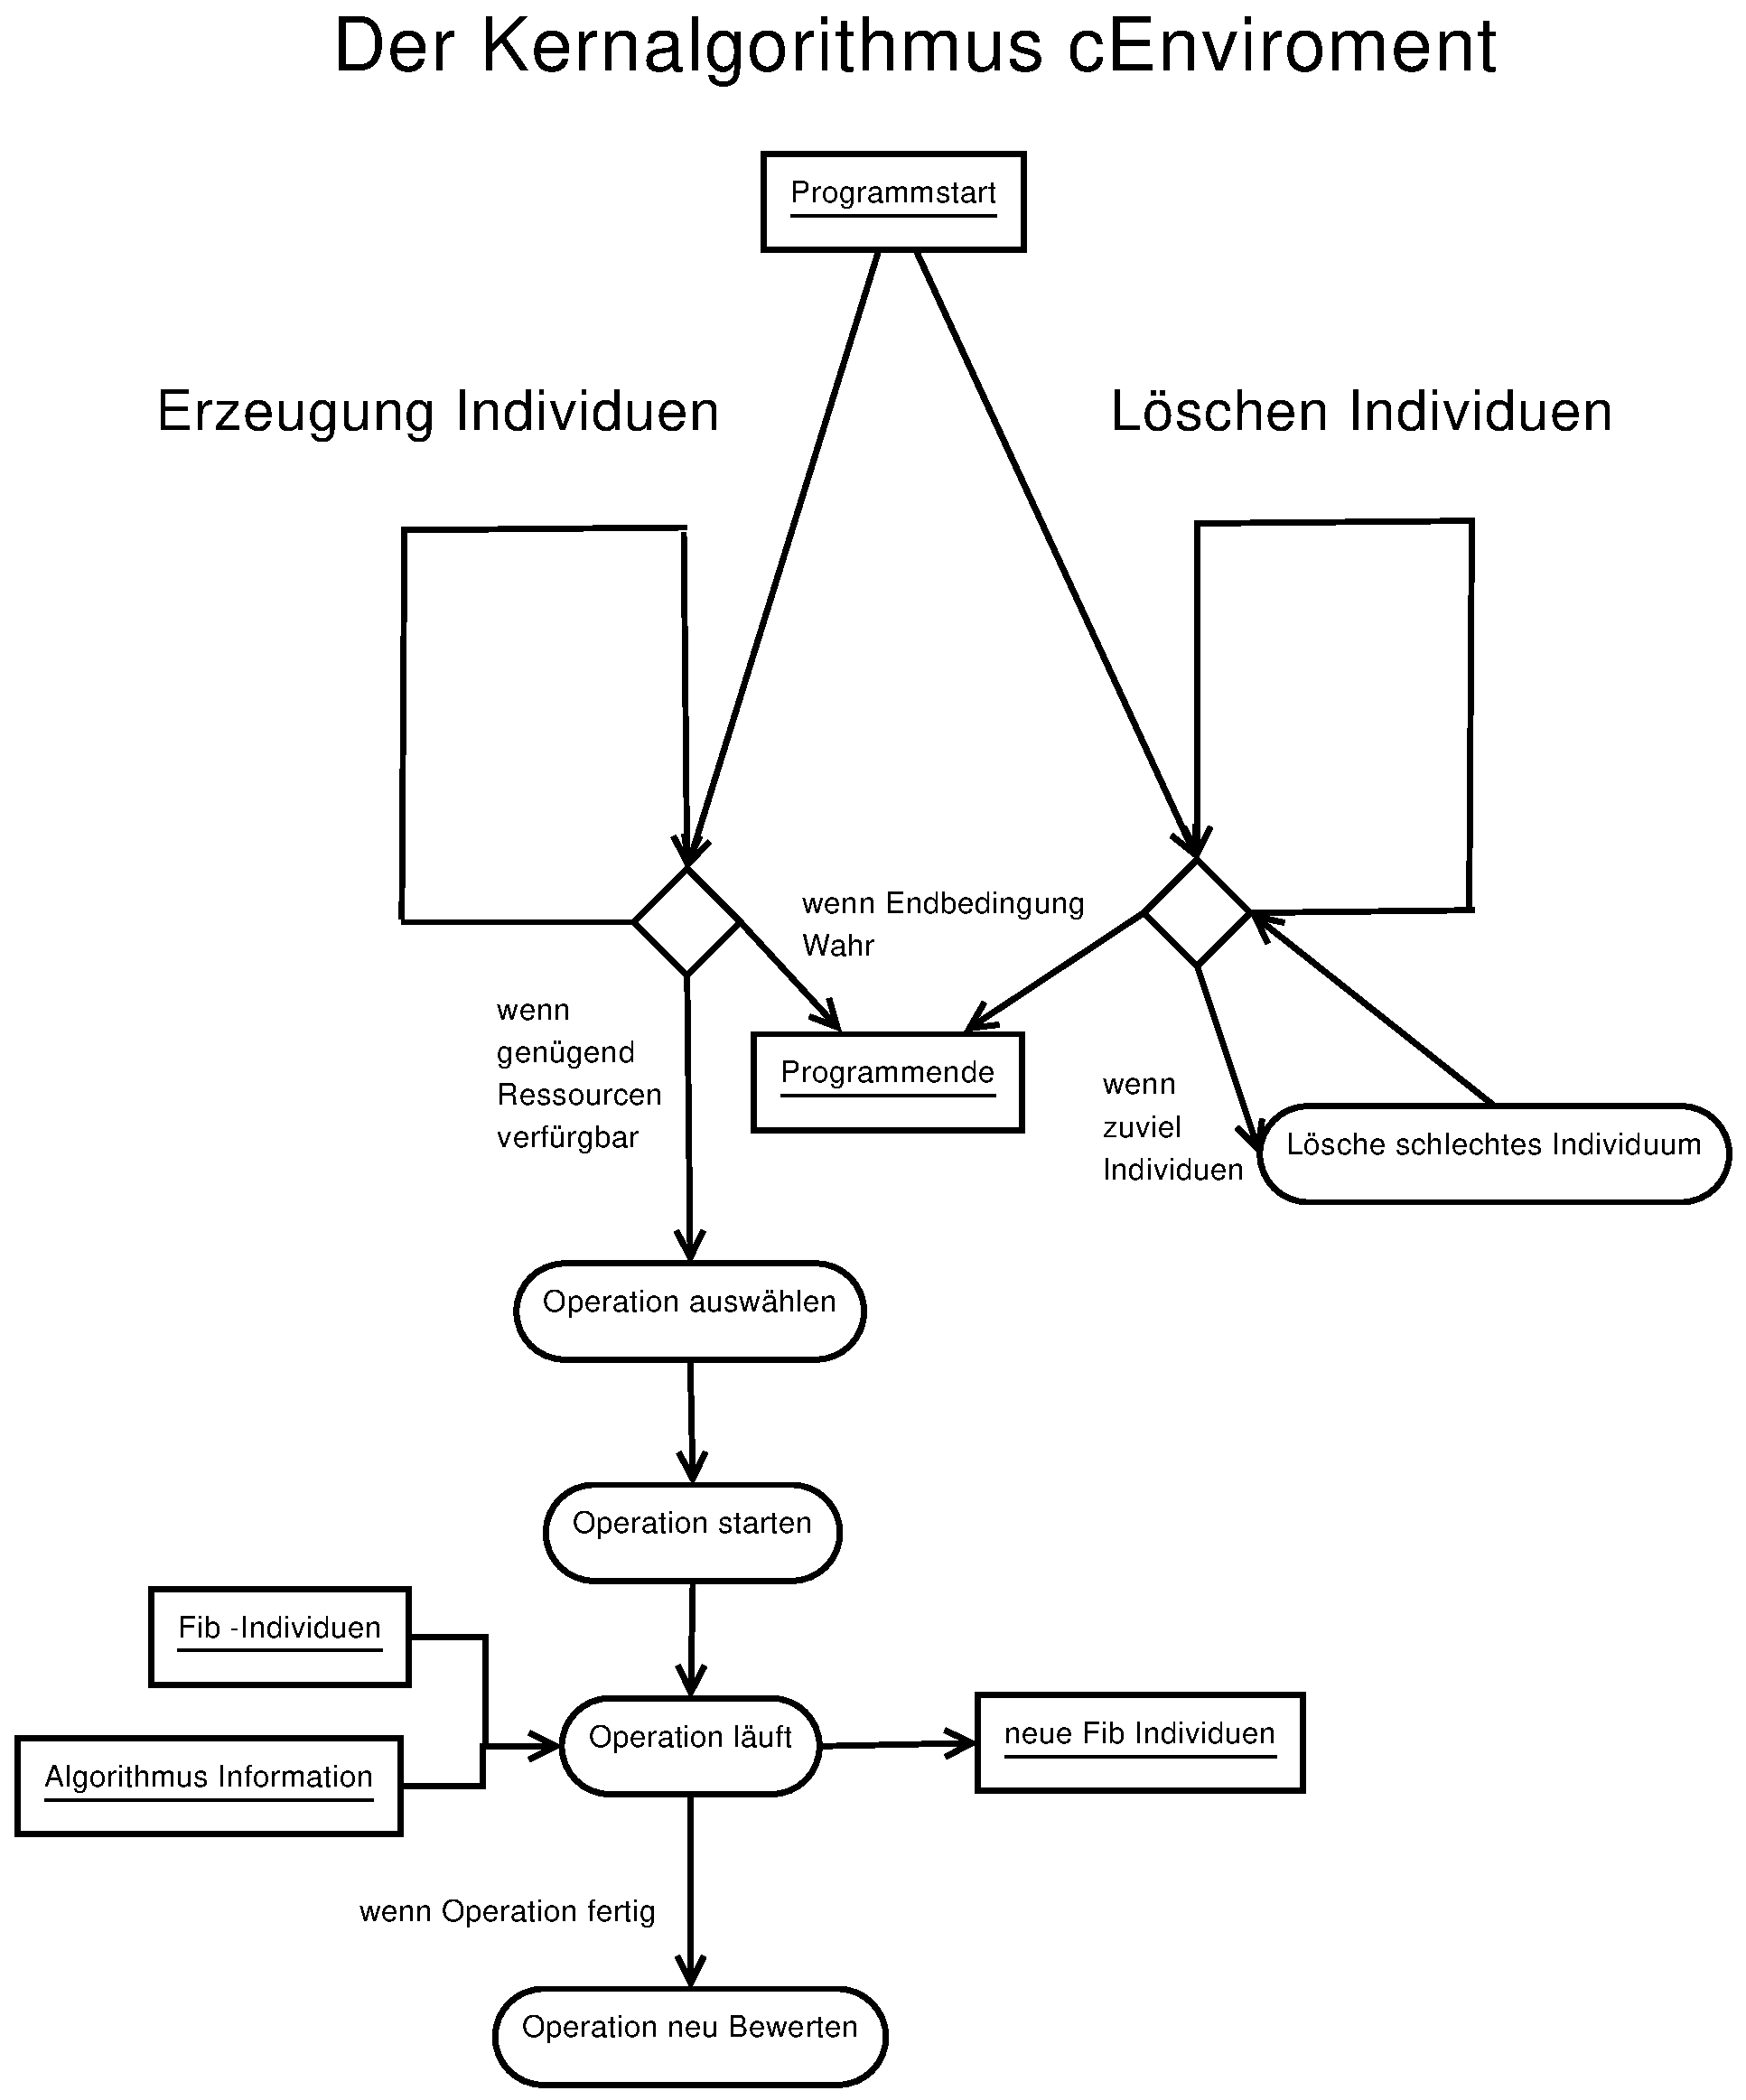
\includegraphics[scale=0.4]{programmablauf}
\end{center}
\caption{Ablaufdiagramm des genetischen Algorithmus}
\label{figEnviromentAlgorithmus}
\end{figure}


\section{Hilfsmethoden}

Hilfsmethoden, die bei der Implementierung hilfreich sind, aber nicht zur eigentlichen Schnittstelle geh"oren, werden nach Bedarf implementiert, hier aber nicht aufgef"uhrt. Sie sollten nach M"oglichkeit von au"sen nicht zugreifbar sein (also \verb|privat| oder \verb|protected| deklariert sein).


\section{Copyright}

Der genetische Algorithmus wird unter die GPL (siehe Abschnitt \ref{secGPL} auf Seite \pageref{secGPL}) gestellt. Er kann also frei angepasst, ver"andert und eingebunden werden, solange das Ergebnis wieder unter der GPL steht. Da der genetische Algorithmus als eigenst"andiges Programm zu sehen ist, sollten die zus"atzlichen Freiheiten der LGPL (siehe Abschnitt \ref{secLGPL} auf Seite \pageref{secLGPL}) f"ur ihn nicht n"otig sein.


\section{Allgemeine Regeln}

F"ur die Implementation des genetischen Algorithmus gibt es ein paar allgemeine Regeln:
\begin{itemize}
 \item Der Algorithmus ist so zu modularisieren, dass Module einfach ausgetauscht werden k"onnen, um ihn an andere Problemstellungen m"oglichst leicht anzupassen zu k"onnen.
 \item Nur der Kernalgorithmus kann Individuen l"oschen.
 \item Nur der Algorithmus bewertet die Operatoren.
 \item Nur der Algorithmus kann eine Operation zum Erzeugen neuer Individuen starten.
 \item Nur der Algorithmus entscheidet, wann er fertig ist und beendet sich. Er kann dabei aber auch auf Signale von au"sen reagieren.
\end{itemize}



\section{Module}

Um den Algorithmus so allgeimein wie m"oglich zu implementieren, werden einige Funktionen von externen Modulen bzw. Klassen realisiert. Im Nachfolgenden werden diese Module vorgestellt.

\subsection{Modul f"ur die Individuen}

Die Individuen sind die zentralen Objekte im Algorithmus. Um verschiedene Problemstellungen bearbeiten zu k"onnen, m"ussen Individuen an die jeweile Problemstellung angepasst werden k"onnen. N"aheres dazu in Abschnitt \ref{secIndividual} auf Seite \pageref{secIndividual}.


\subsection{Modul f"ur die Initialisierung}

Bei Start des Algorithmus (Programmstart) sind einige Aufgaben auszuf"uhren. Dazu geh"ort beispielsweise, dass ein Individuum erzeugt und in die Individuenpopulation (bzw. Individuenliste) als erstes Individuum eingef"ugt wird. N"aheres dazu in Abschnitt \ref{secInitAlgoritmus} auf Seite \pageref{secInitAlgoritmus}.


\subsection{Module f"ur Entscheidungen}

Diese Module werden verwendet, wenn etwas entschieden werden soll. Sie enthalten im Allgemeinen nur eine Funktion, mit der eine Bedingung gepr"uft werden kann.


\subsubsection{Modul f"ur die Ressourcenpr"ufung}

Dieses Modul ist daf"ur zust"andig zu pr"ufen, ob genug System-/Rechnerressourcen vorhanden sind, um weitere Operationen zu starten und auszuf"uhren. N"aheres dazu in Abschnitt \ref{secResourceCheck} auf Seite \pageref{secResourceCheck}.

"Uber das Modul zum Ausw"ahlen einer Operation werden dann neue Operationen gestartet, wenn genug Ressourcen vorhanden sind.


\subsubsection{Modul f"ur die Endbedingung}

Das Modul zum Pr"ufen der Endbedingung zeigt an, wann die Endbedingung erf"ullt ist und der Algorithmus beendet werden soll. N"aheres dazu in Abschnitt \ref{secEndConditionCheck} auf Seite \pageref{secEndConditionCheck}.


\subsubsection{Modul f"ur die maximale Populationsgr"o"se}

Damit die Populationsgr"o"se nicht in das Unendliche anw"achst, muss diese beschr"ankt werden. Um zu bewerten, wann ``zuviele Individuen'' vorhanden sind, dient das Modul f"ur die maximale Populationsgr"o"se. N"aheres dazu in Abschnitt \ref{secMaxPopulation} auf Seite \pageref{secMaxPopulation}.

Das L"oschen von Individuen, um die Population zu beschr"anken, geschieht allerdings mit dem Modul zum L"oschen von Individuen.


\subsection{Module f"ur Vorg"ange}

Die folgenden Module dienen dazu, bestimmte Vorg"ange oder Aufgaben auszuf"uhren bzw. zu erf"ullen.


\subsubsection{Modul zum Bewerten eines Individuums}

Um Individuen vergleichen zu k"onnen, m"ussen diese bewertet werden. Dazu dient das Modul zum Bewerten von Individuen. Jedes neu erzeugte Individuum sollte bewertet werden. Diese Bewertung ist dann zum Individuum zu speichern. Das bedeutet, dass dieses Modul aus zwei Teilen besteht: dem Bewerter und der Bewertung f"ur Individuen.

Mehr zur Bewertung im Abschnitt \ref{secCObjectFitness} auf Seite \pageref{secCObjectFitness} und zum Bewerter im Abschnitt \ref{secCObjectFitnessAlgorithm} auf Seite \pageref{secCObjectFitnessAlgorithm}.


\subsubsection{Modul zum Ausw"ahlen eines guten Individuums}

Einige Operatoren werden Informationen aus bereits existierenden Individuen nutzen wollen, um neue Individuen zu erzeugen. Damit die Individuen unabh"angig von der nachfragenden Operation gew"ahlt werden, ist die Wahl in einem seperaten Modul im Algorithmus zu implementieren. Dieses Modul sollte gute Individuen bevorzugen und austauschbar sein, um auch andere Wahlstrategien leicht einsetzen zu k"onnen. Davon unabh"angig k"onnen Operationen nat"urlich ihre eigenen Wahlmechanismen implementieren.

N"aheres dazu in Abschnitt \ref{secIndividualSelection} auf Seite \pageref{secIndividualSelection}.


\subsubsection{Modul zum L"oschen von Individuen}

Wenn die maximale Populationsgr"o"se "uberschritten ist, m"ussen existierende Individuen gel"oscht werden. Die Auswahl der zu l"oschenden Individuen geschieht "uber ein austauschbares Modul. Die L"oschoperation selbst wird im Kernalgorithmus ausgef"uhrt, um zu vermeiden, dass externe Module "uber eine Schnittstelle Individuen l"oschen k"onnen.

Im Abschnitt \ref{secIndividualDeletionSelection} auf Seite \pageref{secIndividualDeletionSelection} wird dieses Modul beschrieben.


\subsubsection{Modul zum Bewerten einer Operation}

Um zu bestimmen, wie gut Operatoren in bestimmten Situationen arbeiten, m"ussen die Operatoren anhand ihrer Leistung bewertet werden. Da die Art der Operatoren und damit die Bewertungskriterien sich "andern k"onnen, muss dieses Modul austauschbar sein.

Das Modul zum Bewerten von Operatoren wird im Abschnitt \ref{secCOperationFitnessAlgorithmus} auf Seite \pageref{secCOperationFitnessAlgorithmus} beschrieben.


\subsubsection{Modul zum Ausw"ahlen einer Operation}

Um neue Individuen zu erzeugen, m"ussen Operatoren ausgew"ahlt werden. Da die Art der Operatoren sich "andern kann, muss dieses Modul austauschbar sein.

Dieses Modul wird im Abschnitt \ref{secCChoosOperator} auf Seite \pageref{secCChoosOperator} beschrieben.


\section{Inividuen cIndividual}\label{cIndividual}
\label{secIndividual}

Der Algorithmus arbeitet auf der Basis von Individuen. Deshalb sind diese von zentraler Bedeutung f"ur den Algorithmus. Individuen sind es, die er schlie"slich verbessern soll, und das Ergebnis des Algorithmus soll auch ein Individuum sein. Deshalb sind Individuen von zentraler Bedeutung f"ur den Algorithmus.

Die Klasse \verb|cIndividual| repr"asentiert ein Individuum in einer abstrakten Form. Dabei h"alt sie nicht nur die Informationen eines vollst"andigen Objekts, welches verbessert werden soll, sondern auch weitere Angaben. Mit diesen Angaben soll eine beschleunigte Verarbeitung von Individuen erm"oglicht werden.

\bigskip\noindent
Zu den Informationen, welche die Klasse \verb|cFibIndividual| bereitstellt, geh"oren:
\begin{itemize}
 \item das Objekt, welches das Individuum repr"asentiert.
 \item Zusatzinformationen zu einem Individuum \verb|cIndividualInfo| (Siehe Abschnitt \ref{secCIndividualInfo} auf Seite \pageref{secCIndividualInfo})
\end{itemize}


\subsection{Schnittstellenbeschreibung}

\subsubsection{cIndividual}

\textbf{Syntax:} \verb|cIndividual( void * pObject,| \\\verb| const cIndividualInfo & individualInfo )| \\

Der Konstruktor f"ur ein Indiviuum; er erzeugt ein Individuum.

Weder von \verb|pObject| noch von \verb|individualInfo| werden Kopien angefertigt. Beide Objekte werden direkt f"ur das Individuum verwendet.

\bigskip\noindent
\textbf{Eingabeparameter:}
\begin{itemize}
 \item \verb|pObject|: Einen Zeiger auf das Objekt, welches das Individuum repr"asentieren soll.
 \item \verb|individualInfo|: Eine Refernz, auf die Zusatzinformationen f"ur das Objekt.
\end{itemize}

\bigskip\noindent
\textbf{R"uckgabe:} keine


\subsubsection{equal}\index{cIndividual!equal()}\index{cIndividual!Gleichheit}\index{equal()}

\textbf{Syntax:} \verb|boolen equal( const cIndividual &individuum,| \\\verb| bool bCheckIdentifiers=true )| \\
oder \verb|bool operation==( const cIndividual &individuum )|

\bigskip\noindent
Diese Methoden pr"ufen, ob das aktuelle und "ubergebene Individuum gleich sind.

\bigskip\noindent
\textbf{Eingabeparameter:}
\begin{itemize}
 \item \verb|individuum|: Das Individuum, welches gleich zum aktuellen Individuum sein soll.
 \item \verb|bCheckIdentifiers|: Dieser Wert gibt an, ob bei der Gleichheitspr"ufung die beiden Identifier der Objekte (\verb|cIndividualIdentifier| und \verb|cOperationIdentifier|) mit ber"ucksichtigt werden sollen. Wenn er \verb|true| (=wahr) ist, werden die Identifier bei der Pr"ufung mit ber"ucksichtigt. Sonst, wenn er \verb|false| (=falsch) ist, werden die Identifier bei der Pr"ufung nicht ber"ucksichtigt. Es werden dann nur die Strukturen der Individuen auf Gleichheit gepr"uft. Standardwert ist \verb|true| (=wahr), womit auch die Identifier bei der Pr"ufung ber"ucksichtigt werden.
\end{itemize}

\bigskip\noindent
\textbf{R"uckgabe:} Die Methode gibt \verb|true| (=wahr) zur"uck, wenn das aktuelle Individuum gleich dem "ubergebenen Individuum ist, sonst \verb|false| (=falsch).


\subsubsection{getObjekt}\index{cIndividual!getObjekt()}\index{getObjekt()}

\textbf{Syntax:} \verb|void * getObject()|

\bigskip\noindent
Diese Methode gibt einen Zeiger auf das Objekt des Individuums zur"uck. Das Objekt ist der eigentliche Gegenstand des Algorithmus. Auf dem Individuum arbeiten die Operatoren. Das Objekt ist das, was ``verbessert'' werden soll. Die anderen Informationen des Individuums dienen nur dazu, dem Algorithmus Zusatzinformationen zum Objekt zu liefern und die Abarbeitung zu beschleunigen.

\bigskip\noindent
\textbf{Eingabeparameter:} keine

\bigskip\noindent
\textbf{R"uckgabe:} Eine Referenz auf das Objekt des Individuums.


\subsubsection{getInfo}\index{cIndividual!getInfo()}\index{getInfo()}

\textbf{Syntax:} \verb|cIndividualInfo * getInfo()|

\bigskip\noindent
Diese Methode liefert einen Zeiger auf die Zusatzinformationen des Individuums zur"uck. Dies sind Informationen zum Objekt des Individuums, welche dem Algorithmus und den Operatoren die Arbeit erleichtern. Sie enthalten auch allgemeine Informationen (wie z. B. die Erzeugungszeit des Objekts).

\bigskip\noindent
\textbf{Eingabeparameter:} keine

\bigskip\noindent
\textbf{R"uckgabe:} Einen Zeiger auf die Zusatzinformationen des Individuums.


\subsubsection{getClassName}\index{cIndividual!getClassName()}\index{getClassName()}

\textbf{Syntax:} \verb|string getClassName() const|

\bigskip\noindent
Diese Funktion gibt den Klassennamen ''cIndividual`` des Individuumobjekts zur"uck.

In abgeleiteten Klassen sollte diese Methode immer "uberschrieben werden, so dass der jeweilige Klassenname zur"uckgegeben wird.

\bigskip\noindent
\textbf{Eingabeparameter:} keine

\bigskip\noindent
\textbf{R"uckgabe:} Den Klassennamen ''cIndividual`` des Individuumobjekts.



\section{Zusatzinformationen zu einem Individuum cIndividualInfo}
\label{secCIndividualInfo}

Die Klasse \verb|cIndividualInfo| stellt zus"atzliche Informationen zu einem Individuum (bzw. Objekt) bereit.

\bigskip\noindent
Zu den Informationen, welche die Klasse \verb|cIndividualInfo| bereitstellt, geh"oren:
\begin{itemize}
 \item ein Wahrheitswert (boolean), der angibt, ob das Individuum noch lebt bzw. ob das Objekt noch existiert oder es tot ist, bzw. das Objekt gel"oscht wurde. Die Klasse \verb|cIndividualInfo| kann noch "uber das Ableben/ L"oschen des Individuums hinaus leben, um beispielsweise sp"atere statistiche Auswertungen zu erlauben.
 \item ein Identifier \verb|cIndividualIdentifier| f"ur das Individuum. Dies ist eine eindeutige nat"urliche Zahl f"ur das Inividuum und eine Zahl f"ur die genetischen Algorithmusinstanz, in dem es erzeugt wurde. Die genetische Algorithmusinstanz ben"otigt einen seperaten Identifier, da es vorgesehen ist, dass Individuen zwischen genetischen Algorithmusinstanzen migrieren k"onnen (zur Klasse \verb|cIndividualIdentifier| siehe Abschnitt \ref{secCIndividuumIdentifier} auf Seite \pageref{secCIndividuumIdentifier}).
 \item die Fitness des Objekts (zur Klasse \verb|cObjectFitness| siehe Abschnitt \ref{secCObjectFitness} auf Seite \pageref{secCObjectFitness}).
 \item der (lokale) Zeitpunkt der Erzeugung des Objekts.
 \item die Anzahl der bisher vom Algorithmus ausgef"uhrten Operationen.
 \item eine Liste mit den Identifieren der direkten Vorfahren des Inividuums. Diese k"onnen beispielsweise f"ur Heuristiken interessant sein.
 \item der Operatorname der Operation, mit der das Objekt erzeugt wurde, inklusive einem freien Feld (eine Unicodezeichenkette), in dem vom Operator weitere Eintr"age vorgenommen werden k"onnen. In dem freien Feld kann beispielsweise von der Operation eingetragen werden, welche Unteroperatoren sie mit welchen Parametern zur Erzeugung des Objekts benutzt hat. Diese Informationen (Name und freies Feld) werden als zwei Zeichenketten abgespeichert.
 \item der Identifier \verb|cOperationIdentifier| der erzeugenden Operation.
 \item der zur Erzeugung ben"otigte Aufwand $A$ (als Systemunab"ahngige Gleitkommazahl). Dieser wird in Abschnitt \ref{secOperationCost} auf Seite \pageref{secOperationCost} beschrieben.
 \item die Fitness des besten Individuums zum Erzeugungszeitpunkt, um die Verbesserung einsch"atzen zu k"onnen, welche das Individuum darstellt.
\end{itemize}

Die Zusatzinformationen \verb|cIndividualInfo| zu einem Individuum sollten auch nach dem L"oschen des Individuums/Objekts persistent auf der Festplatte erhalten bleiben. Daf"ur ist ein Limit f"ur den zur Verf"ugung stehenden Festplattenplatz zu setzen. Wird dieses Limit f"ur die Zusatzinformationen "uberschritten, sind die "altesten Zusatzinformationen von der Platte zu l"oschen, bis das Limit wieder eingehalten wird.
Auf diese Weise stehen Informationen zur Verf"ugung, um die Operationen zu bewerten.


\subsection{Der Aufwand von Operationen}
\label{secOperationCost}

Der Aufwand von Operatoren sollte systemunabh"angig ermittelt werden, um auch zwischen einzelnen Systemen den Aufwand vergleichen zu k"onnen. Dies ist n"otig, da der Algorithmus auch verteilt auf mehreren Systemen laufen kann und auch dann die Operatoren vergleichbar bleiben sollten. Der Aufwand wird mit einer Gleitkommazahl repr"asentiert.

Der Aufwand f"ur Operationen wird ermittelt, indem die Prozessorzeit ("CPU Time``) der Operation mit einem durch einen Benchmark ermittelten Wert multipliziert wird.

%TODO besser?: alle erzeugten Individuen haben operation cost

Wenn eine Operation mehrere Individuen erzeugt, muss der gesamte Aufwand der Operation "uber diese Individuen verteilt werden. Die Summe der Aufw"ande aller von der Operation erzeugten Individuen ist gleich oder gr"o"ser dem Gesamtaufwand der Operation, welche diese Individuen erzeugt hat. Kein Individuum darf aber weniger Aufwand zugeschrieben werden als $1/16$ des Durchschnittsaufwands der Individuen zu seiner Operation. Wenn also eine Operation $I$ Individuen erzeugte und dazu einen Gesamtaufwand von $A$ ben"otigte, darf keinem Individuum ein Aufwand $A_i$ kleiner als $A/I*1/16$ zugeschrieben werden. Mit dieser Regel soll vermieden werden, dass Operatoren einzelne Individuen ''sch"onrechnen``.


\subsubsection{Benchmark}

Der Benchmark dient zum Ermitteln eines Benchmarkwertes, mit dem die Prozessorzeit von Operationen skaliert werden kann, um so eine Systemunabh"angigkeit der Aufwandwerte zu gew"ahrleisten.

Daf"ur wird der Benchmark jedes Mal ermittelt, wenn sich seit dem letzten Benchmark leistungsrelevante Rechnerkomponenten ge"andert haben.

\bigskip\noindent
Zu den leistungsrelevanten Rechnerkomponenten geh"oren:
\begin{itemize}
 \item CPU (Art, Anzahl, Taktung); alle an der Berechnung beteiligten CPU's sind zu ber"ucksichtigen, eventuell also auch Grafikprozessoren
 \item Mainbord
 \item Arbeitsspeicher (Gr"o"se, Art, Taktung); aller an der Berechnung beteiligter Arbeitsspeicher ist zu ber"ucksichtigen, eventuell also auch Arbeitsspeicher der Grafikkarte
 \item neue Compilierung des Algorithmus (neue Algorithmusversion oder Compilerversion)
\end{itemize}

Um den Benchmarkwert zu ermitteln, wird auf einem festen Objekt/Individuum eine Reihe von deterministischen Operationen ausgef"uhrt und die daf"ur verbrauchte Prozessorzeit $T_B$ ("CPU Time``) gemessen. Das Reziproke der Prozessorzeit ($1/T_B=B$) ist dann der Benchmarkwert $B$, mit dem die Prozessorzeit ("CPU Time``) von Operationen $T_{O}$ multipliziert wird, um ihren Aufwand zu ermitteln ($A=T_O*B=T_O/T_B$ mit $A$ als systemunab"ahngige Gleitkommazahl f"ur den Aufwand der Operation).


\subsection{Schnittstellenbeschreibung}

\subsubsection{cIndividualInfo}\index{Individuum!cIndividualInfo}\index{cIndividualInfo}

\textbf{Syntax:} \verb|cIndividualInfo(| \\\verb| unsigned long ulAlgorithmusIdentifier,| \\\verb| list<cIndividualIdentifier> liIdentifierOfParents,| \\\verb| cObjectFitness fitness,| \\\verb| string szOperationName, string szOperationInfo,| \\\verb| cOperationIdentifier operationIdentifier,| \\\verb| time creationTime, double dOperationCost,| \\\verb| const cObjectFitness * pFitnessOfBestAtCreationTime )| \\

Der Konstruktor f"ur ein Objekt f"ur die Zusatzinformationen zu einem Individuum.

Das erzeugte Individuum lebt immer.

Nur "uber den Konstruktor des Objekts f"ur Zusatzinformationen zu einem Individuum k"onnen die Daten dessen gesetzt werden. F"ur \verb|cIndividualInfo| gibt es keine ''set``-Methoden.

Der Identifier des Individuums wird automatisch erzeugt. Zusammen mit dem Identifier des Algorithmus \verb|ulAlgorithmusIdentifier| kann damit das Individuum eindeutig identifiziert werden.

\bigskip\noindent
\textbf{Eingabeparameter:}
\begin{itemize}
 \item \verb|ulAlgorithmusIdentifier|: Der Identifier des Algorithmus.
 \item \verb|liIdentifierOfParents|: Eine Liste mit den Identifiern der direkten Vorfahren des Inividuums. Die Operation hat diese benutzt, um das Individuum zu erzeugen.
 \item \verb|fitness|: Die Fitness des Objekts.
 \item \verb|szOperationName|: Der Name des Operators, mit dem das Individuum erzeugt wurde.
 \item \verb|szOperationInfo|: Weitere Informationen zur Operation, mit dem das Individuum erzeugt wurde.
 \item \verb|operationIdentifier|: Der Identifier der Operation, mit der das Individuum erzeugt wurde.
 \item \verb|creationTime|: Der Zeitpunkt zu dem das Individuum erzeugt wurde.
 \item \verb|dOperationCost|: Der zur Erzeugung des Individuums ben"otigte Aufwand.
 \item \verb|pFitnessOfBestAtCreationTime|: Die Fitness des besten Individuums im Algorithmus zum Zeitpunkt, als das zu \verb|cIndividualInfo| geh"orende Individuum erzeugt wurde.
\end{itemize}

\bigskip\noindent
\textbf{R"uckgabe:} keine


\subsubsection{getIdentifier}\index{cIndividualInfo!getIdentifier()}\index{getIdentifier()}

\textbf{Syntax:} \verb|cIndividualIdentifier getIdentifier() const|

\bigskip\noindent
Diese Funktion liefert den Identifizierer des Individuums. Dies ist eine eindeutige nat"urliche Zahl f"ur das Inividuum und eine Zahl f"ur die genetische Algorithmusinstanz, in dem es erzeugt wurde (siehe Abschnitt \ref{secCIndividuumIdentifier} auf Seite \pageref{secCIndividuumIdentifier}).

\bigskip\noindent
\textbf{Eingabeparameter:} keine

\bigskip\noindent
\textbf{R"uckgabe:} Den Identifizierer des Individuums.


\subsubsection{kill}\index{cIndividualInfo!kill()}\index{kill()}

\textbf{Syntax:} \verb|bool kill()|

\bigskip\noindent
Diese Methode deklariert das Individuum f"ur tot bzw. nicht lebendig.

\bigskip\noindent
\textbf{Eingabeparameter:} keine

\bigskip\noindent
\textbf{R"uckgabe:} Wenn das Individuum get"otet werden konnte (bzw. es vorher nicht tot war), wird \verb|true| (=wahr) zur"uckgegeben, sonst \verb|false| (=falsch).


\subsubsection{isLiving}\index{cIndividualInfo!isLiving()}\index{isLiving()}

\textbf{Syntax:} \verb|bool isLiving() const|

\bigskip\noindent
Diese Funktion gibt zur"uck, ob das Individuum noch lebt.

\bigskip\noindent
\textbf{Eingabeparameter:} keine

\bigskip\noindent
\textbf{R"uckgabe:} Wenn das Individuum lebt, wird \verb|true| (=wahr) zur"uckgegeben, sonst \verb|false| (=falsch).


\subsubsection{getIdentifiersOfParents}\index{cIndividualInfo!getIdentifiersOfParents()}\index{getIdentifiersOfParents()}

\textbf{Syntax:} \verb|list<cIndividualIdentifier>| \\\verb| getIdentifiersOfParents() const|

\bigskip\noindent
Diese Funktion gibt eine Liste mit den Identifiern der Elternindividuen zur"uck. Elternindividuen sind Individuen von, denen die Operation Informationen benutzt hat, um das Individuum zu erzeugen.
(Siehe Abschnitt \ref{secCIndividuumIdentifier} auf Seite \pageref{secCIndividuumIdentifier}.)

\bigskip\noindent
\textbf{Eingabeparameter:} keine

\bigskip\noindent
\textbf{R"uckgabe:} Eine Liste mit den Identifiern der Elternindividuen.


\subsubsection{getFitness}\index{cIndividualInfo!getFitness()}\index{getFitness()}

\textbf{Syntax:} \verb|const cObjectFitness * getFitness() const|

\bigskip\noindent
Diese Funktion gibt eine Referenz auf die Fitness des Individuums zur"uck (siehe Abschnitt \ref{secCObjectFitness} auf Seite \pageref{secCObjectFitness}).

\bigskip\noindent
\textbf{Eingabeparameter:} keine

\bigskip\noindent
\textbf{R"uckgabe:} Eine Referenz auf die Fitness des Individuums.


\subsubsection{getOperatorName}\index{cIndividualInfo!getOperatorName()}\index{getOperatorName()}

\textbf{Syntax:} \verb|string getOperatorName() const|

\bigskip\noindent
Diese Funktion gibt den Namen des Operators zur"uck, von dem das Individuum erstellt wurde.

\bigskip\noindent
\textbf{Eingabeparameter:} keine

\bigskip\noindent
\textbf{R"uckgabe:} Den Namen des Operators, von dem das Individuum erstellt wurde.


\subsubsection{getOperatorInfo}\index{cIndividualInfo!getOperatorInfo()}\index{getOperatorInfo()}

\textbf{Syntax:} \verb|string getOperatorInfo() const|

\bigskip\noindent
Diese Funktion gibt weitere Informationen zu der Operation zur"uck, von der das Individuum erstellt wurde. Dies k"onnen beispielsweise Erstellungsparameter sein.

\bigskip\noindent
\textbf{Eingabeparameter:} keine

\bigskip\noindent
\textbf{R"uckgabe:} Weitere Informationen zu der Operation, von der das Individuum erstellt wurde.


\subsubsection{getOperatorIdentifier}\index{cIndividualInfo!getOperatorIdentifier()}\index{getOperatorIdentifier()}

\textbf{Syntax:} \verb|cOperationIdentifier getOperatorIdentifier() const|

\bigskip\noindent
Diese Funktion gibt den Identifier der Operation zur"uck, von der das Individuum erstellt wurde (siehe Abschnitt \ref{secCOperationIdentifier} auf Seite \pageref{secCOperationIdentifier}).

\bigskip\noindent
\textbf{Eingabeparameter:} keine

\bigskip\noindent
\textbf{R"uckgabe:} Den Identifier der Operation, von der das Individuum erstellt wurde.


\subsubsection{getCreationTime}\index{cIndividualInfo!getCreationTime()}\index{getCreationTime()}

\textbf{Syntax:} \verb|time getCreationTime() const|

\bigskip\noindent
Diese Funktion gibt den Zeitpunkt zur"uck, an dem das Individuum erzeugt wurde.

\bigskip\noindent
\textbf{Eingabeparameter:} keine

\bigskip\noindent
\textbf{R"uckgabe:} Den Zeitpunkt, an dem das Individuum erzeugt wurde.


\subsubsection{getOperationCost}\index{cIndividualInfo!getOperationCost()}\index{getOperationCost()}

\textbf{Syntax:} \verb|double getOperationCost() const|

\bigskip\noindent
Diese Funktion gibt den Aufwand zur"uck, der zur Erzeugung des Individuums ben"otigt wurde
(siehe Abschnitt \ref{secOperationCost} auf Seite \pageref{secOperationCost}).

\bigskip\noindent
\textbf{Eingabeparameter:} keine

\bigskip\noindent
\textbf{R"uckgabe:} Den Aufwand, der zur Erzeugung des Individuums ben"otigt wurde.


\subsubsection{getFitnessOfBestAtCreationTime}\index{cIndividualInfo!getFitnessOfBestAtCreationTime()}\index{getFitnessOfBestAtCreationTime()}

\textbf{Syntax:} \verb|const cObjectFitness *| \\\verb| getFitnessOfBestAtCreationTime() const|

\bigskip\noindent
Diese Funktion gibt eine Referenz auf die Fitness des besten Individuums im Algorithmus zum Erzeugungszeitpunkt des entsprechenden zum \verb|cIndividualInfo| Objekt geh"orenden Individuums zur"uck.

\bigskip\noindent
\textbf{Eingabeparameter:} keine

\bigskip\noindent
\textbf{R"uckgabe:} Eine Referenz auf die Fitness des besten Individuums im Algorithmus zum Erzeugungszeitpunkt des entsprechenden zum \verb|cIndividualInfo| Objekt geh"orenden Individuums.



\section{Die Fitness von Individuen cObjectFitness}
\label{secCObjectFitness}

Die Klasse \verb|cObjectFitness| stellt die Fitness eines Objekts (bzw. Individuums) dar. Sie ist die Basisklasse f"ur alle Klassen f"ur die Fitness von Objekten. Von der Klasse \verb|cObjectFitness| selbst oder einer abgeleiteten Klasse kann keine Instanz direkt erzeugt werden. Instanzen von Objekten der Klasse \verb|cObjectFitness| k"onnen nur durch die Berechnung der Fitness mit den Klassen f"ur die Algorithmen \verb|cObjectFitnessAlgorithm| (siehe Abschnitt \ref{secCObjectFitnessAlgorithm} auf Seite \pageref{secCObjectFitnessAlgorithm}) oder durch das Laden einer existierenden Fitness aus einem Datenstrom erzeugt werden.

Zu den Fitnessinformationen geh"ort die Gesamtfitness des Objekts. Abgeleitete Klasse k"onnen aber mehrere Fitnesswerte enthalten.


\subsection{Schnittstellenbeschreibung}

\subsubsection{cObjectFitness}\index{Individuum!cObjectFitness}\index{cObjectFitness}

\textbf{Syntax:} \verb|cObjectFitness( double dFittness,| \\\verb| cObjectFitnessAlgorithm *pObjectFitnessAlgorithmus=NULL )| \\

Der Konstruktor f"ur ein Fitnessobjekt f"ur ein Individuum.

Nur "uber den Konstruktor des Fitnessobjekt k"onnen die Daten dessen gesetzt werden. Es gibt f"ur \verb|cObjectFitness| keine ''set``-Methoden.

\bigskip\noindent
\textbf{Eingabeparameter:}
\begin{itemize}
 \item \verb|dFittness|: Der Fitnesswert f"ur das Inividuum.
 \item \verb|pObjectFitnessAlgorithmus|: Einen Zeiger auf das Algorithmusobjekt \verb|cObjectFitnessAlgorithm|, mit dem die Fitness erzeugt wurde. Standardwert ist der Nullpointer \verb|NULL| um anzuzeigen, dass kein Algorithmusobjekt diese Fitness erzeugt hat.
\end{itemize}

\bigskip\noindent
\textbf{R"uckgabe:} keine


\subsubsection{getFitness}\index{cObjectFitness!getFitness()}\index{getFitness()}

\textbf{Syntax:} \verb|double getFitness() const|

\bigskip\noindent
Diese Funktion gibt die Fitness des zugeh"origen Individuums zur"uck.

In abgeleiteten Klassen gibt diese Methode die Gesamtfitness des Individuums zur"uck.
Dieser Wert sollte linear sein, d. h. wenn der Wert halb so gro"s ist, sollte das Individuum auch nur halb so gut sein.

\bigskip\noindent
\textbf{Eingabeparameter:} keine

\bigskip\noindent
\textbf{R"uckgabe:} Die Fitness des zugeh"origen Individuums.


\subsubsection{getClassName}\index{cObjectFitness!getClassName()}\index{getClassName()}

\textbf{Syntax:} \verb|string getClassName() const|

\bigskip\noindent
Diese Funktion gibt den Klassennamen ''cObjectFitness`` des Fitnessobjekts zur"uck.

In abgeleiteten Klassen sollte diese Methode immer "uberschrieben werden, so dass der jeweilige Klassenname zur"uckgegeben wird.

\bigskip\noindent
\textbf{Eingabeparameter:} keine

\bigskip\noindent
\textbf{R"uckgabe:} Den Klassennamen ''cObjectFitness`` des Fitnessobjekts.


\subsubsection{getFitnessAlgorithmus}\index{cObjectFitness!getFitnessAlgorithmus()}\index{getFitnessAlgorithmus()}

\textbf{Syntax:} \verb|const cObjectFitnessAlgorithm * | \\\verb| getFitnessAlgorithmus() const|

\bigskip\noindent
Diese Funktion gibt einen Zeiger auf das Algorithmusobjekt (siehe Abschnitt \ref{secCObjectFitnessAlgorithm} auf Seite \pageref{secCObjectFitnessAlgorithm}) zur"uck, mit das Fitnessobjekte erzeugt wurde. F"ur Fitnessobjekte vom Typ \verb|cObjectFitness| wird eine Referenz auf das Algorithmusobjekt vom Typ \verb|cObjectFitnessAlgorithm| zur"uckgegeben.

In abgeleiteten Klassen sollte diese Methode immer "uberschrieben werden, so dass das jeweilige Algorithmusobjekt zur"uckgegeben wird.

\bigskip\noindent
\textbf{Eingabeparameter:} keine

\bigskip\noindent
\textbf{R"uckgabe:} Zur"uckgegeben wird eine Referenz auf das Algorithmusobjekt vom Typ \verb|cObjectFitnessAlgorithm|.


\subsubsection{Gleichheit von cObjectFitness Objekten}\index{cObjectFitness!Vergleiche}\index{Vergleiche}

\textbf{Syntax:} \verb|bool equal( const cObjectFitness &fitness ) const|\\
\verb|bool operation==( const cObjectFitness &fitness ) const|

\bigskip\noindent
Diese Methoden vergleichen zwei \verb|cObjectFitness| Objekte. Wenn der Typ und die Fitnesswerte im "ubergebenen Fitnessobjekt gleich dem des aktuellen Objekts vom Typ \verb|cObjectFitness| sind, wird \verb|true| (=wahr) zur"uckgegeben, sonst \verb|false| (=falsch).

\bigskip\noindent
\textbf{Eingabeparameter:} keine

\bigskip\noindent
\textbf{R"uckgabe:} Wenn das "ubergebene \verb|cObjectFitness| Objekt gleich dem aktuellen \verb|cObjectFitness| Objekt ist, wird \verb|true| (=wahr) zur"uckgegeben, ansonsten wird \verb|false| (=falsch) zur"uckgegeben.


\subsubsection{Kleiner Vergleich von cObjectFitness Objekten}\index{cObjectFitness!Kleiner Vergleich}\index{Kleiner Vergleich}

\textbf{Syntax:} \verb|bool operation<( const cObjectFitness &fitness )| \\\verb| const|

\bigskip\noindent
Dieser Operator vergleicht zwei \verb|cObjectFitness| Objekte. Wenn die Gesamtfitnesswert im "ubergebenen Objekt gr"o"ser als das aktuelle \verb|cObjectFitness| ist, wird \verb|true| (=wahr) zur"uckgegeben, ansonsten \verb|false| (=falsch).

\bigskip\noindent
\textbf{Eingabeparameter:} keine

\bigskip\noindent
\textbf{R"uckgabe:} Wenn der Gesamtfitnesswert im "ubergebenen Objekt gr"o"ser als das aktuelle \verb|cObjectFitness| ist, wird \verb|true| (=wahr) zur"uckgegeben, ansonsten \verb|false| (=falsch).




\section{cIndividualIdentifier}
\label{secCIndividuumIdentifier}

Die Klasse \verb|cIndividualIdentifier| stellt einen Identifier f"ur das Individuum bereit. Dies ist eine eindeutige nat"urliche Zahl f"ur das Inividuum und eine nat"urliche Zahl f"ur die genetische Algorithmusinstanz, in der es erzeugt wurde. Die genetische Algorithmusinstanz ben"otigt einen seperaten Identifier, da es vorgesehen ist, dass Individuen zwischen genetischen Algorithmusinstanzen migrieren k"onnen.

Einen Identifier f"ur ein Individuum sollte es nur maximal einmal geben. Weder auf anderen Rechnern noch f"ur andere Algorithmusl"aufe sollten Identifier doppelt erzeugt werden.


\subsection{Schnittstellenbeschreibung}

\subsubsection{cIndividualIdentifier}\index{Individuum!cIndividualIdentifier}\index{cIndividualIdentifier}

\textbf{Syntax:} \verb|cIndividualIdentifier(| \\\verb| unsigned long ulAlgorithmusIdentifier )| \\

Der Konstruktor f"ur einen Identifier f"ur ein Individuum. Er erzeugt einen eindeutigen Identifier f"ur ein Individuum.

\bigskip\noindent
\textbf{Eingabeparameter:}
\begin{itemize}
 \item \verb|ulAlgorithmusIdentifier|: Der Identifier des Algorithmus.
\end{itemize}

\bigskip\noindent
\textbf{R"uckgabe:} keine


\subsubsection{getNoIndividualIdentifier}\index{cIndividualIdentifier!getNoIndividualIdentifier()}\index{getNoIndividualIdentifier()}

\textbf{Syntax:} \verb|static cIndividualIdentifier &| \\\verb| getNoIndividualIdentifier()| \\

Diese Methode gibt eine Referenz f"ur einen \verb|cIndividualIdentifier| zur"uck, der f"ur kein Individuum steht.

Dieser Identifier ist kleiner als alle anderen \verb|cIndividualIdentifier| und sollte niemals einem Individuum zugeordnet werden.

\bigskip\noindent
\textbf{Eingabeparameter:} keine

\bigskip\noindent
\textbf{R"uckgabe:} Zur"uckgegeben wird eine Referenz auf einen fest definierten Identifier \verb|cIndividualIdentifier|, der f"ur kein Individuum steht.


\subsubsection{Vergleiche von cIndividualIdentifier Objekten}\index{cIndividualIdentifier!Vergleiche}\index{Vergleiche}

\textbf{Syntax:} \verb|bool equal(| \\\verb| const cIndividualIdentifier &identifier ) const|\\
\verb|bool operation==(| \\\verb| const cIndividualIdentifier &identifier ) const|

\bigskip\noindent
Diese Methoden vergleichen zwei \verb|cIndividualIdentifier| Objekte. Wenn das "ubergebene Objekt gleich dem aktuellen \verb|cIndividualIdentifier| Objekt ist, wird \verb|true| (=wahr) zur"uckgegeben, ansonsten \verb|false| (=falsch).

\bigskip\noindent
\textbf{Eingabeparameter:} keine

\bigskip\noindent
\textbf{R"uckgabe:} Wenn das "ubergebene \verb|cIndividualIdentifier| Objekt gleich dem aktuellen \verb|cIndividualIdentifier| Objekt ist, wird \verb|true| (=wahr) zur"uckgegeben, ansonsten \verb|false| (=falsch).


\section{Algorithmus f"ur einen Bewerter von Individuen cObjectFitnessAlgorithm}
\label{secCObjectFitnessAlgorithm}

Die Klasse \verb|cObjectFitnessAlgorithm| ist die Basisklasse der Bewerter f"ur die Fitness von Individuen. Von ihr selbst kann keine Instanz erzeugt werden.


\subsection{Schnittstellenbeschreibung}

\subsubsection{cObjectFitnessAlgorithm}\index{cObjectFitnessAlgorithm}

\textbf{Syntax:} \verb|cObjectFitnessAlgorithm()| \\

Der Konstruktor f"ur ein Objekt zum Bewerter von Individuen.

\bigskip\noindent
\textbf{Eingabeparameter:} keine

\bigskip\noindent
\textbf{R"uckgabe:} keine

\subsubsection{cObjectFitnessAlgorithm}\index{cObjectFitnessAlgorithm}

\textbf{Syntax:} \verb|cObjectFitnessAlgorithm(| \\\verb| const cIndividual & original )| \\

Der Konstruktor f"ur ein Objekt zum Bewerter von Individuen.

\bigskip\noindent
\textbf{Eingabeparameter:}
\begin{itemize}
 \item \verb|original|: Eine Referenz auf das Individuum, welches als Originalindividuum gesetzt werden soll.
\end{itemize}

\bigskip\noindent
\textbf{R"uckgabe:} keine


\subsubsection{evalueFitness}\index{cObjectFitnessAlgorithm!evalueFitness()}\index{evalueFitness()}

\textbf{Syntax:} \verb|cObjectFitness * evalueFitness(| \\\verb| const cIndividual  &individual  )| \\

Diese Methode berechnet die Fitness eines Individuums \verb|individual|. Sie wird nicht von \verb|cObjectFitnessAlgorithm| implementiert und muss daher in den von \verb|cObjectFitnessAlgorithm| abgeleiteten Klassen implementiert werden.

\bigskip\noindent
\textbf{Eingabeparameter:}
\begin{itemize}
 \item \verb|individual|: Eine Referenz auf das Individuum, welches bewertet werden soll.
\end{itemize}

\bigskip\noindent
\textbf{R"uckgabe:} Zur"uckgegeben wird ein Zeiger auf ein Fitnessobjekt f"ur die Fitness des Individuums \verb|individual|, berechnet nach dem aktuellen Individuumbewerter bez"uglich des gesetzten Originalindividuums.


\subsubsection{setOriginalIndividual}\index{cObjectFitnessAlgorithm!setOriginalIndividual()}\index{setOriginalIndividual()}

\textbf{Syntax:} \verb|bool setOriginalIndividual(| \\\verb| const cIndividual  &original )| \\

Diese Methode wird das Originalindividuum gesetzt. Bez"uglich dieses Individuums werden andere Individuen vom Bewerteralgorithmus bewertet.
%TODO weg: Die Methode wird nicht von \verb|cObjectFitnessAlgorithm| implementiert und muss daher in den von \verb|cObjectFitnessAlgorithm| abgeleiteten Klassen implementiert werden.

Das zu setzende Originalindividuum \verb|original| muss den richtigen Typ f"ur den Bewerter haben, um gesetzt werden zu k"onnen. Ist der Typ falsch wird das Individuum \verb|original| nicht als Origianl gesetzt und \verb|false| zur"uckgegeben.

\bigskip\noindent
\textbf{Eingabeparameter:}
\begin{itemize}
 \item \verb|original|: Eine Referenz auf das Individuum, welches als Originalindividuum gesetzt werden soll.
\end{itemize}

\bigskip\noindent
\textbf{R"uckgabe:} Wenn das "ubergebene Individuum als Originalindividuum gesetzt wurde, wird \verb|true| (=wahr) zur"uckgegeben, ansonsten \verb|false| (=falsch).


\subsubsection{getOriginalIndividual}\index{cObjectFitnessAlgorithm!getOriginalIndividual()}\index{getOriginalIndividual()}

\textbf{Syntax:} \verb|cIndividual * getOriginalIndividual()| \\

Diese Methode gibt eine Referenz auf das Originalindividuum zur"uck. Bez"uglich dieses Individuums werden andere Individuen vom Bewerteralgorithmus bewertet.

\bigskip\noindent
\textbf{Eingabeparameter:} keine

\bigskip\noindent
\textbf{R"uckgabe:} Zur"uckgegeben wird eine Referenz auf das Originalindividuum.


\subsubsection{getClassName}\index{cObjectFitnessAlgorithm!getClassName()}\index{getClassName()}

\textbf{Syntax:} \verb|string getClassName()| \\

Diese Methode gibt eine Zeichenkette mit dem Klassennamen des aktuellen Bewerters f"ur Individuen zur"uck.

\bigskip\noindent
\textbf{Eingabeparameter:} keine

\bigskip\noindent
\textbf{R"uckgabe:} Zur"uckgegeben wird eine Zeichenkette mit dem Klassennamen des aktuellen Bewerters f"ur Individuen.


\subsubsection{getBestFitness}\index{cObjectFitnessAlgorithm!getBestFitness()}\index{getBestFitness()}

\textbf{Syntax:} \verb|const cObjectFitness * getBestFitness() const| \\

Diese Methode gibt die bestm"ogliche Fitness eines Individuums bez"uglich des Originalobjekts zur"uck. Diese Fitness zeichnet aus, dass es nicht m"oglich ist, eine bessere Fitness zu generieren.

Diese Fitness entspricht im Normalfall einem Individuum, welches das Originalobjekt perfekt wiedergibt und dabei keine Recourcen verbraucht.

\bigskip\noindent
\textbf{Eingabeparameter:} keine

\bigskip\noindent
\textbf{R"uckgabe:} Zur"uckgegeben wird ein Zeiger auf die bestm"ogliche Fitness eines Individuums bez"uglich des Originalobjekts oder der Nullzeiger \verb|NULL|, wenn diese nicht berechnet werden kann.


\subsubsection{getWorstCaseFitness}\index{cObjectFitnessAlgorithm!getWorstCaseFitness()}\index{getWorstCaseFitness()}

\textbf{Syntax:} \verb|const cObjectFitness * getWorstCaseFitness() const| \\

Diese Methode gibt die schlechtestm"ogliche Fitness eines Individuums bez"uglich des Originalobjekts zur"uck. Diese Fitness zeichnet aus, dass sie immer erreicht werden kann.

Im Normalfall wird der Algorithmus die Fitness des Originalindividuums zur"uckgeben, da dieses ja schon in der entsprechenden Repr"asentation vorliegt und verbessert werden soll.

Der Algorithmus kann dennoch durch \verb|evalueFitness()| Fitnessobjekte generieren, die noch schlechter sind.

Es wird der Nullzeiger \verb|NULL| zur"uckgegeben, wenn die schlechtestm"ogliche Fitness nicht berechnet werden kann. Dies kann beispielsweise der Fall sein, wenn kein Originalobjekt f"ur den Algorithmus gesetzt wurde.

\bigskip\noindent
\textbf{Eingabeparameter:} keine

\bigskip\noindent
\textbf{R"uckgabe:} Zur"uckgegeben wird ein Zeiger auf die schlechtestm"ogliche Fitness eines Individuums bez"uglich des Originalobjekts oder der Nullzeiger \verb|NULL|, wenn diese nicht berechnet werden kann.




\section{Initialisieren des Algorithmus cInitEnviroment}
\label{secInitAlgoritmus}

Die Klasse \verb|cInitEnviroment| ist die Basisklasse zur Initialisierung des Algorithmus. Von der Klasse \verb|cInitEnviroment| werden alle Klassen zur Initialisierung des Algorithmus abgeleitet. Von \verb|cInitEnviroment| selbst k"onnen allerdings keine Instanzen erzeugt werden, da eine allgemeine Initialisierung nich m"oglich ist.

F"ur die Initialisierung steht die Methode \verb|initEnviroment()| bereit.

Die Initialisierung umfasst:
\begin{itemize}
 \item die Bereitstellung des Originalindividuums. Die Daten f"ur das Originalindividuum k�nnen der von \verb|cInitEnviroment| abgeleiteten Klasse "uber ihren Konstruktor "ubergeben werden.
 \item Erzeugen und Einf"ugen mindestens eines Individuums f"ur und in die Population. So hat der Algorithmus von Anfang an ein Individuum zum Zur"uckgeben. Diese Individuen k"onnen auch aus einem fr"uheren Lauf des Algorithmus kommen und/oder aus einer Datei geladen werden.
 \item Aufrufen, wenn vorhanden, des Initialsierungsoperators \verb|cInitOperator|.
\end{itemize}


\subsection{Schnittstellenbeschreibung}

\subsubsection{cInitEnviroment}\index{cEnviroment!cInitEnviroment()}\index{cInitEnviroment()}

\textbf{Syntax:} \verb|cInitEnviroment()| \\

Der Konstruktor f"ur das Initialisierungsobjekt des Algorithmus (\verb|cEnviroment| siehe Abschnitt \ref{secCEnviroment} auf Seite \pageref{secCEnviroment}).

\bigskip\noindent
\textbf{Eingabeparameter:} keine

\bigskip\noindent
\textbf{R"uckgabe:} keine


\subsubsection{initEnviroment}\index{cInitEnviroment!initEnviroment()}\index{initEnviroment()}

\textbf{Syntax:} \verb|bool initEnviroment()| \\

Diese Methode initialisiert den Algorithmus.

Bevor die Initialisierung ausgef"uhrt werden kann, m"u"sen die gew"unschten Parameter zur Initialisierung "uber die ''set``-Methoden oder/und die Konstruktoren des von \verb|cInitEnviroment| abgeleiteten Objekts gesetzt werden.

Weiterhin muss gepr"uft werden, ob die Initialisierung zur aktuellen Instanz von \verb|cEnviroment| passt. Dazu geh"ort beispielsweise, dass der Typ der bei der Initialisierung erzeugten Individuen zur aktuellen \verb|cEnviroment| Instanz passt.

\bigskip\noindent
\textbf{Eingabeparameter:} keine

\bigskip\noindent
\textbf{R"uckgabe:} Wenn der Algorithmus \verb|cEnviroment| initialisiert wurde, wird \verb|true| (=wahr) zur"uckgegeben, ansonsten \verb|false| (=falsch).


\subsubsection{getClassName}\index{cInitEnviroment!getClassName()}\index{getClassName()}

\textbf{Syntax:} \verb|string getClassName()| \\

Diese Methode gibt eine Zeichenkette mit dem Klassennamen des aktuellen Objekts zur"uck.

\bigskip\noindent
\textbf{Eingabeparameter:} keine

\bigskip\noindent
\textbf{R"uckgabe:} Zur"uckgegeben wird eine Zeichenkette mit dem Klassennamen des aktuellen Bewerters f"ur Individuen.



\section{Pr"ufen der Endbedingung mit cEndConditionCheck}
\label{secEndConditionCheck}

Die Klasse \verb|cEndConditionCheck| und von ihr abgeleitete Klassen stellen die Methode \verb|endConditionCheck()| zum Pr"ufen der Endbedingung bereit. Wenn die Methode \verb|endConditionCheck()| wahr (=\verb|true|) zur"uckgibt, sollte sich der Algorithmus beenden. Die Methode  \verb|endConditionCheck()| sollte in regelm"a"sigen Abst"anden (im Zehntelsekundenbereich) vom Algorithmus aufgerufen werden, so dass sich der Algorithmus zeitnah beendet.

\bigskip\noindent
Bei folgenden Bedingungen ist die Endbedingung erf"ullt und die Methode zur Pr"ufen der Endbedingung \verb|endConditionCheck()| gibt wahr \verb|true| zur"uck:
\begin{itemize}
 \item Es wird ein Signal zum Beenden empfangen (unter Linux: HUP=1, QUIT=3, TERM=15).
 \item Es wird eine maximale Fitness "uberschritten.
 \item Eine maximal Anzahl von Operatorenaufrufen (bzw. Operationen) wird "uberschritten.
 \item Eine maximale Prozessorlaufzeit ist "uberschritten.
 \item Eine maximale Laufzeit (Realzeit) ist "uberschritten.
 \item Ein bestimmter Zeitpunkt ist "uberschritten.
\end{itemize}


\subsection{Schnittstellenbeschreibung}


\subsubsection{cEndConditionCheck}\index{cEnviroment!cEndConditionCheck()}\index{cEndConditionCheck()}

\textbf{Syntax:} \verb|cEndConditionCheck()| \\

Der Konstruktor f"ur ein Objekt zum Pr"ufen der Endbedingung f"ur den Algorithmus (\verb|cEnviroment| siehe Abschnitt \ref{secCEnviroment} auf Seite \pageref{secCEnviroment}).

In dem neu konstruierten Objekt ist nur die Bedingung des ''Signal zum Beenden`` aktiviert. Alle anderen Endbedingungen m"ussen "uber die ''set``-Methoden gesetzt werden.

\bigskip\noindent
\textbf{Eingabeparameter:} keine

\bigskip\noindent
\textbf{R"uckgabe:} keine


\subsubsection{endConditionCheck}\index{cEndConditionCheck!endConditionCheck()}\index{endConditionCheck()}

\textbf{Syntax:} \verb|bool endConditionCheck()| \\

Diese Methode gibt zur"uck, ob der Algorithmus beendet werden soll. Der Algorithmus sollte beendet werden, wenn eine der oben aufgef"uhrten Bedingung erf"ullt ist.

\bigskip\noindent
\textbf{Eingabeparameter:} keine

\bigskip\noindent
\textbf{R"uckgabe:} Wenn der Algorithmus \verb|cEnviroment| beendet werden soll, wird \verb|true| (=wahr) zur"uckgegeben, ansonsten \verb|false| (=falsch).


\subsubsection{getClassName}\index{cInitEnviroment!getClassName()}\index{getClassName()}

\textbf{Syntax:} \verb|string getClassName()| \\

Diese Methode gibt eine Zeichenkette mit dem Klassennamen des aktuellen Objekts zur"uck.

\bigskip\noindent
\textbf{Eingabeparameter:} keine

\bigskip\noindent
\textbf{R"uckgabe:} Zur"uckgegeben wird eine Zeichenkette mit dem Klassennamen des aktuellen Bewerters f"ur Individuen.


\subsubsection{getMaxFitness}\index{cEndConditionCheck!getMaxFitness()}\index{getMaxFitness()}

\textbf{Syntax:} \verb|cObjectFitness *getMaxFitness() const| \\

Diese Methode gibt eine Referenz auf ein Fitnessobjekt zur"uck, dessen Wert von den Individuen nicht "uberschritten werden soll. Ist die "ubergebene Referenz \verb|NULL| wird die Pr"ufung auf die maximale Fitness nicht ausgef"uhrt.

Die Fitnessobjekte der Individuen werden mit dem Fitnessobjekt der maximalen Fitnessbedingung "uber den kleineren Operator der Fitnessobjekte verglichen. Wird also die Endbedingung mit der \verb|endConditionCheck()| Methode gepr"uft, und die maximale Fitnessbedingung ist aktiv (bzw. das maximale Fitnessobjekt ist nicht \verb|NULL|), dann wird das Individuum mit der h"ochsten Fitness im Algorithmus ermittelt und dessen Fitness mit dem maximalen Fitnessobjekt verglichen. Ist die Fitness des maximalen Fitnessobjekts kleiner als die des ermittelten Individuums, wird von \verb|endConditionCheck()| wahr (=\verb|true|) zur"uckgegeben.

\bigskip\noindent
\textbf{Eingabeparameter:} keine

\bigskip\noindent
\textbf{R"uckgabe:} Eine Referenz auf ein Fitnessobjekt, dessen Wert von den Individuen nicht "uberschritten werden soll.


\subsubsection{setMaxFitness}\index{cEndConditionCheck!setMaxFitness()}\index{setMaxFitness()}

\textbf{Syntax:} \verb|bool setMaxFitness( cObjectFitness *fitness=NULL )| \\

Diese Methode setzt das Fitnessobjekt, dessen Wert von den Individuen nicht "uberschritten werden soll. Ist die "ubergebene Referenz \verb|fitness| gleich \verb|NULL|, wird die Pr"ufung auf die maximale Fitness nicht ausgef"uhrt. Das Objekt zur "ubergebenen Referenz wird, wenn vorhanden, dabei kopiert.

Die Fitnessobjekte der Individuen werden mit dem Fitnessobjekt der maximalen Fitnessbedingung "uber den kleineren Operator der Fitnessobjekte verglichen. Wird also die Endbedingung mit der \verb|endConditionCheck()| Methode gepr"uft, und die maximale Fitnessbedingung ist aktiv (bzw. das maximale Fitness Objekt ist nicht \verb|NULL|), dann wird das Individuum mit der h"ochsten Fitness im Algorithmus ermittelt und dessen Fitness mit dem maximalen Fitnessobjekt verglichen. Ist die Fitness des maximalen Fitnessobjekts kleiner als die des ermittelten Individuums, wird von \verb|endConditionCheck()| wahr (=\verb|true|) zur"uckgegeben.

\bigskip\noindent
\textbf{Eingabeparameter:}
\begin{itemize}
 \item \verb|fitness|: Eine Referenz auf das Fitnessobjekt, dessen Wert von den Individuen nicht "uberschritten werden soll. Ist die "ubergebene Referenz \verb|fitness| gleich \verb|NULL|, wird die Pr"ufung auf die maximale Fitness nicht ausgef"uhrt. Standardwert von \verb|fitness| ist \verb|NULL|, um die die maximale Fitnesspr"ufung nicht auszuf"uhren.
\end{itemize}

\bigskip\noindent
\textbf{R"uckgabe:} Wenn die maximale Fitness auf \verb|fitness| gesetzt wurde, wird \verb|true| (=wahr) zur"uckgegeben, ansonsten \verb|false| (=falsch).


\subsubsection{getMaxOperationCalls}\index{cEndConditionCheck!getMaxOperationCalls()}\index{getMaxOperationCalls()}

\textbf{Syntax:} \verb|unsigned long getMaxOperationCalls() const| \\

Diese Methode gibt die maximale Anzahl der Opertorenaufrufe (=Operationen) zur"uck. Ist dieser Wert $0$ , wird die Pr"ufung auf die maximale Operationen nicht ausgef"uhrt bzw. es k"onnen beliebig viele Operationen ausgef"uhrt werden.

Wird die Endbedingung mit der \verb|endConditionCheck()| Methode gepr"uft, wenn die maximale Anzahl von Operationen gr"o"ser als $0$ ist und die Anzahl der Opertionen, die der Algorithmus bisher ausgef"uhrt hat, gr"o"ser als die maximale Anzahl von Operationen ist, wird von \verb|endConditionCheck()| wahr (=\verb|true|) zur"uckgegeben.

\bigskip\noindent
\textbf{Eingabeparameter:} keine

\bigskip\noindent
\textbf{R"uckgabe:} Die maximale Anzahl der Opertorenaufrufe (=Operationen).


\subsubsection{setMaxOperationCalls}\index{cEndConditionCheck!setMaxOperationCalls()}\index{setMaxOperationCalls()}

\textbf{Syntax:} \verb|bool setMaxOperationCalls(| \\\verb| unsigned long ulMaxCalls=0 )| \\

Diese Methode setzt die maximale Anzahl von Opertorenaufrufen (=Operationen). Ist dieser Wert $0$ (Standardwert), wird die Pr"ufung auf die maximale Operationen nicht ausgef"uhrt bzw. es k"onnen beliebig viele Operationen ausgef"uhrt werden.

Wird die Endbedingung mit der \verb|endConditionCheck()| Methode gepr"uft, wenn die maximale Anzahl von Operationen gr"o"ser als $0$ ist und die Anzahl der Operationen, die der Algorithmus bisher ausgef"uhrt hat, gr"o"ser als die maximale Anzahl von Operationen ist, wird von \verb|endConditionCheck()| wahr (=\verb|true|) zur"uckgegeben.

\bigskip\noindent
\textbf{Eingabeparameter:}
\begin{itemize}
 \item \verb|ulMaxCalls|: Die maximale Anzahl von Opertorenaufrufen (=Operationen), welche gesetzt werden soll. Ist der "ubergebene Wert \verb|ulMaxCalls| gleich $0$, wird die Pr"ufung auf die maximale Operationen nicht ausgef"uhrt bzw. es k"onnen beliebig viele Operationen ausgef"uhrt werden. Standardwert von \verb|ulMaxCalls| ist $0$, um die maximale Operationenpr"ufung nicht auszuf"uhren.
\end{itemize}

\bigskip\noindent
\textbf{R"uckgabe:} Wenn der die maximale Anzahl von Operationen auf \verb|ulMaxCalls| gesetzt wurde, wird \verb|true| (=wahr) zur"uckgegeben, ansonsten \verb|false| (=falsch).


\subsubsection{getMaxCpuRuntime}\index{cEndConditionCheck!getMaxCpuRuntime()}\index{getMaxCpuRuntime()}

\textbf{Syntax:} \verb|double getMaxCpuRuntime() const| \\

Diese Methode gibt die maximale CPU-Zeit in Sekunden zur"uck, die der Algorithmus verbrauchen darf. Ist dieser Wert negativ, wird die Pr"ufung auf die maximale CPU-Zeit nicht ausgef"uhrt bzw. der Algorithmus kann beliebig viel CPU-Zeit verbrauchen.

Wird die Endbedingung mit der \verb|endConditionCheck()|-Methode gepr"uft, wenn die maximale CPU-Zeit gr"o"ser als $0$ ist und die aktuelle CPU-Zeit, die der Algorithmus bisher verbraucht hat, gr"o"ser als die CPU-Zeit ist, wird von von der Methode \verb|endConditionCheck()| wahr (=\verb|true|) zur"uckgegeben.

\bigskip\noindent
\textbf{Eingabeparameter:} keine

\bigskip\noindent
\textbf{R"uckgabe:} Die maximale CPU-Zeit, die der Algorithmus verbrauchen darf.


\subsubsection{setMaxCpuRuntime}\index{cEndConditionCheck!setMaxCpuRuntime()}\index{setMaxCpuRuntime()}

\textbf{Syntax:} \verb|bool setMaxCpuRuntime( double dMaxCpuTime=-1.0 )| \\
%TODO Olli: 14471


Diese Methode setzt die maximale CPU-Zeit in Sekunden, die der Algorithmus verbrauchen darf. Ist dieser Wert negativ (Standardwert), wird die Pr"ufung auf die maximale CPU-Zeit nicht ausgef"uhrt, bzw. der Algorithmus kann beliebig viel CPU-Zeit verbrauchen.

Wird die Endbedingung mit der \verb|endConditionCheck()| Methode gepr"uft, wenn die maximale CPU-Zeit gr"o"ser als $0$ ist und die aktuelle CPU-Zeit, die der Algorithmus bisher verbraucht hat, gr"o"ser als die CPU-Zeit ist, wird von der Methode \verb|endConditionCheck()| wahr (=\verb|true|) zur"uckgegeben.

\bigskip\noindent
\textbf{Eingabeparameter:}
\begin{itemize}
 \item \verb|dMaxCpuTime|: Die maximale CPU-Zeit in Sekunden, die der Algorithmus verbrauchen darf. Ist der "ubergebene Wert \verb|dMaxCpuTime| negativ, wird die Pr"ufung auf die maximale CPU-Zeit nicht ausgef"uhrt, bzw. der Algorithmus kann beliebig viel CPU-Zeit verbrauchen. Standardwert von \verb|dMaxCpuTime| ist $-1.0$, um die maximale CPU-Zeitpr"ufung nicht auszuf"uhren.
\end{itemize}

\bigskip\noindent
\textbf{R"uckgabe:} Wenn der die maximale CPU-Zeit auf \verb|dMaxCpuTime| gesetzt wurde, wird \verb|true| (=wahr) zur"uckgegeben, ansonsten \verb|false| (=falsch).


\subsubsection{getMaxRuntime}\index{cEndConditionCheck!getMaxRuntime()}\index{getMaxRuntime()}

\textbf{Syntax:} \verb|double getMaxRuntime() const| \\

Diese Methode gibt die maximale Laufzeit in Sekunden zur"uck, die der Algorithmus verbrauchen darf. Die Laufzeit ist die Zeit, die vergeht, w"ahrend der Algorithmus l"auft (das bedeuted nicht: w"arend der Algorithmus gestartet ist und arbeitet). Ist dieser Wert negativ, wird die Pr"ufung auf die maximale Laufzeit nicht ausgef"uhrt, bzw. der Algorithmus kann beliebig viel Laufzeit verbrauchen.

Wird die Endbedingung mit der \verb|endConditionCheck()| Methode gepr"uft, wenn die maximale Laufzeit gr"o"ser als $0$ ist und die Laufzeit, die der Algorithmus bisher verbraucht hat, gr"o"ser als die Laufzeit ist, wird von \verb|endConditionCheck()| wahr (=\verb|true|) zur"uckgegeben.

\bigskip\noindent
\textbf{Eingabeparameter:} keine

\bigskip\noindent
\textbf{R"uckgabe:} Zur"uckgegeben wird die maximale Laufzeit, die der Algorithmus verbrauchen darf.


\subsubsection{setMaxRuntime}\index{cEndConditionCheck!setMaxRuntime()}\index{setMaxRuntime()}

\textbf{Syntax:} \verb|bool setMaxRuntime( double dMaxTime=-1.0 )| \\

Diese Methode setzt die maximale Laufzeit in Sekunden, die der Algorithmus verbrauchen darf. Laufzeit ist die Zeit die vergeht, w"ahrend der Algorithmus l"auft (das bedeuted nicht: w"arend der Algorithmus gestartet ist und arbeitet). Ist dieser Wert negativ (Standardwert), wird die Pr"ufung auf die maximale Laufzeit nicht ausgef"uhrt, bzw. der Algorithmus kann beliebig viel Laufzeit verbrauchen.

Wird die Endbedingung mit der \verb|endConditionCheck()| Methode gepr"uft, wenn die maximale Laufzeit gr"o"ser als $0$ ist und die Laufzeit, die der Algorithmus bisher verbraucht hat, gr"o"ser als die Laufzeit ist, wird von \verb|endConditionCheck()| wahr (=\verb|true|) zur"uckgegeben.

\bigskip\noindent
\textbf{Eingabeparameter:}
\begin{itemize}
 \item \verb|dMaxTime|: Die maximale Laufzeit in Sekunden, die der Algorithmus verbrauchen darf. Ist der "ubergebene Wert \verb|dMaxTime| negativ, wird die Pr"ufung auf die maximale Laufzeit nicht ausgef"uhrt, bzw. der Algorithmus kann beliebig viel Laufzeit verbrauchen. Standardwert von \verb|dMaxTime| ist $-1.0$, um die maximale Laufzeitpr"ufung nicht auszuf"uhren.
\end{itemize}

\bigskip\noindent
\textbf{R"uckgabe:} Wenn der die maximale Laufzeit auf \verb|dMaxTime| gesetzt wurde, wird \verb|true| (=wahr) zur"uckgegeben, sonst \verb|false| (=falsch).


\subsubsection{getMaxDate}\index{cEndConditionCheck!getMaxDate()}\index{getMaxDate()}

\textbf{Syntax:} \verb|time getMaxDate() const| \\

Diese Methode gibt das Enddatum (inclusive dem Zeitpunkt) zur"uck, bis zu dem der Algorithmus laufen darf. Ist dieser Wert $0$ (als unkonvertierter Datumswert), wird die Pr"ufung auf das Enddatum nicht ausgef"uhrt, bzw. der Algorithmus kann beliebig lange laufen.

Wird die Endbedingung mit der \verb|endConditionCheck()| Methode gepr"uft, wenn das Enddatum gr"o"ser als $0$ ist und das aktuelle Datum gr"o"ser/ sp"ater als das Enddatum ist, wird von \verb|endConditionCheck()| wahr (=\verb|true|) zur"uckgegeben.

\bigskip\noindent
\textbf{Eingabeparameter:} keine

\bigskip\noindent
\textbf{R"uckgabe:} Zur"uckgegeben wird das Enddatum, bis zu dem der Algorithmus laufen darf.


\subsubsection{setMaxDate}\index{cEndConditionCheck!setMaxDate()}\index{setMaxDate()}

\textbf{Syntax:} \verb|bool setMaxDate( time tMaxDate=0 )| \\

Diese Methode setzt das Enddatum (inclusive dem Zeitpunkt), bis zu dem der Algorithmus laufen darf. Ist dieser Wert $0$ (als unkonvertierter Datumswert), wird die Pr"ufung auf das Enddatum nicht ausgef"uhrt, bzw. der Algorithmus kann beliebig lange laufen.

Wird die Endbedingung mit der \verb|endConditionCheck()| Methode gepr"uft, wenn das Enddatum gr"o"ser als $0$ ist und das aktuelle Datum gr"o"ser/ sp"ater als das Enddatum ist, wird von \verb|endConditionCheck()| wahr (=\verb|true|) zur"uckgegeben.

\bigskip\noindent
\textbf{Eingabeparameter:}
\begin{itemize}
 \item \verb|tMaxDate|: Das Enddatum (inclusive dem Zeitpunkt), bis zu dem der Algorithmus laufen darf. Ist der "ubergebene Wert \verb|tMaxDate| $0$ (als unkonvertierter Datumswert), wird die Pr"ufung auf das Enddatum nicht ausgef"uhrt, bzw. der Algorithmus kann beliebig lange laufen. Standardwert von \verb|tMaxDate| ist $0$, um die Enddatumspr"ufung nicht auszuf"uhren.
\end{itemize}

\bigskip\noindent
\textbf{R"uckgabe:} Wenn der das Enddatum auf \verb|tMaxDate| gesetzt wurde, wird \verb|true| (=wahr) zur"uckgegeben, sonst \verb|false| (=falsch).


\section{Kernalgorithmus cEnviroment}\index{cEnviroment}
\label{secCEnviroment}

Der Kernalgorithmus \verb|cEnviroment| implementiert den genetischen Algorithmus unter zuhilfenahme der Bewerter und Operatoren. Es kann vom Kernalgorithmus bzw. der Umwelt immer nur eine Instanz (im g"ultigen Prozessraum) existieren.

Im Kernalgorithmus werden zwei Schleife solange ausgef"uhrt, bis die Endbedingung zutrift oder sie, "uber die Methode \verb|stop()|, gestoppt wird.

Eine Schleife dient zum Erzeugen von Individuen und die andere zum L"oschen von Individuen. Daf"ur werden Operationen ausgew"ahlt (das Ausw"ahlen geschieht mit Hilfe von \verb|cChoosOperation| abgeleiteten Klassen) und gestartet, solange noch gen"ugend Rechnerresourcen (Pr"ufung mit von \verb|cResouceCheck| abgeleiteten Klassen) vorhanden sind. Gestartete Operationen werden vermerkt. Wird eine Operation beendet, so werden die von ihr erzeugten Individuen gepr"uft und es wird die Operation mit den von ihr erzeugten Individuen bewertet.
Wenn eine Operation kein Individum erzeugt, wird f"ur sie vom Kernalgorithmus ein Dummyindividuum eingef"ugt und die Operation bez"uglich dieser bewertet. Dieses Dummyindividuum besteht nur aus Individueninformationen \verb|cIndividualInfo| "uber ein totes Individuum. Die Fitness dieses Dummyindividuum ist die minimal m"ogliche Fitness.

Sollte eine Operation schon sehr lange laufen, wird gepr"uft ob die Operation noch reagiert (mit der \verb|isRunning()| Methode der Operation). Dann wird eventuell versucht die Operation mit ihrer \verb|stop()|-Methode zu beenden. Wenn auch dies nicht zum Erfolg f"uhrt, wird der Prozess in dem die Operation l"auft beendet.

Der Kernalgorithmus ist generisch f"ur ein von der Klasse \verb|cIndividual| abgeleiteten Individuentyp geschrieben.


\subsection{Schnittstelle}


\subsubsection{cEnviroment}\index{cEnviroment}

\textbf{Syntax:} \verb|protected cEnviroment()| \\

Der Konstruktor f"ur ein Kernalgorithmusobjekt. Diese Methode kann nicht von au"serhalb der \verb|cEnviroment| Klasse oder von ihr abgeleiteten Klassen aufgerufen werden. Da der Kernalgorithmus nur einmal existieren kann (bzw. ein singelton Objekt ist), kann nur eine Instanz von ihm existieren. Diese Instanz des Kernalgorithmus kann "uber die Methode \verb|getInstance()| erhalten werden.

"Uber die \verb|setParameter()| Methode die Parameter des Kernalgorithmus gesetzt werden, bevor dieser gestartet werden kann (mit \verb|start()|).

\bigskip\noindent
\textbf{Eingabeparameter:} keine

\bigskip\noindent
\textbf{R"uckgabe:} keine


\subsubsection{setParameter}\index{cEnviroment!setParameter()}\index{setParameter()}

\textbf{Syntax:} \verb|static bool setParameter( const cInitEnviroment * pInit,| \\\verb| const cObjectFitnessAlgorithm * pObjectFitnessAlgorithmus,| \\\verb| const cEndConditionCheck * pEndCondition=NULL ,| \\\verb| const cIndividualSelection * pIndividualSelection=NULL,| \\\verb| const cMaximumReached * pMaximumIndividuals=NULL,| \\\verb| const cSelectIndividualToDelete * pSelectIndividualToDelete=NULL,| \\\verb| const cOperatorFitnessAlgorithm * pOperationFitnessAlgorithm=NULL,| \\\verb| const cChoosOperator * pChoosOperator=NULL,| \\\verb| const cResourceCheck * pResourceCheck=NULL )|
| \\

Diese Methode setzt die Parameter f"ur den Kernalgorithmus.

Erst nachdem die Parameter gesetzt wurden kann der Kernalgorithmus (mit \verb|start()|) gestartet werden.

Wenn ein oder mehrere Parameter nicht gesetzt werden k"onnen, wird \verb|false| (=falsch) zur"uckgegeben. In diesem Fall werden die Parameter des Algorithmus nicht ver"andert, d. h. der Aufruf von \verb|setParameter| bewirkt dann keine "Anderung.

Alle Parameter sind Zeiger, da f"ur sie auch abgeleitete Klassen verwendet werden k"onnen. Von allen Parametern werden Kopien erzeugt und f"ur den Algorithmus verwendet.

\bigskip\noindent
\textbf{Eingabeparameter:}
\begin{itemize}
 \item \verb|pInit|: Das Objekt zum Initialisieren des Kernalgorithmus. (siehe Abschnitt \ref{secInitAlgoritmus} auf Seite \pageref{secInitAlgoritmus})
 \item \verb|pObjectFitnessAlgorithmus|: Mit diesem Objekt wird der Typ der Fitnessobjekte der Individuen im Kernalgorithmus festgelegt. Das Objekt stellt den Algorithmus bzw. eine Funktion zum Erzeugen der Fitness f"ur Individuen bereit. (siehe Abschnitt \ref{secCObjectFitnessAlgorithm} auf Seite \pageref{secCObjectFitnessAlgorithm})
 \item \verb|pEndCondition|: Das Objekt zum Pr"ufen der Endbedingung f"ur den Kernalgorithmus. (siehe Abschnitt \ref{secEndConditionCheck} auf Seite \pageref{secEndConditionCheck}) Als Standardobjekt (wenn \verb|NULL|) wird ein mit dem Standardkonstruktor der Klasse \verb|cEndConditionCheck| erzeugtes Objekt genommen.
 \item \verb|pIndividualSelection|: Diese Objekt dient der Auswahl von guten Individuen aus der Individuenmenge des Kernalgorithmus. (siehe Abschnitt \ref{secIndividualSelection} auf Seite \pageref{secIndividualSelection}) Als Standardobjekt (wenn \verb|NULL|) wird ein mit dem Standardkonstruktor der Klasse \verb|cIndividualSelectionWeel| erzeugtes Objekt genommen.
 \item \verb|pMaximumIndividuals|: Mit diesem Objekt wird eine Funktion bereitgestellt, "uber welche die maximale Anzahl von Individuen im Kernolgorithmus begrenzt werden kann. (siehe Abschnitt \ref{secCMaximumReached} auf Seite \pageref{secCMaximumReached}) Als Standardobjekt (wenn \verb|NULL|) wird ein mit dem Standardkonstruktor der Klasse \verb|cMaximumReached| erzeugtes Objekt genommen.
 \item \verb|pSelectIndividualToDelete|: Diese Objekt dient der Auswahl von Individuen aus der Individuenmenge des Kernalgorithmus, welche gel"oscht werden sollen. (siehe Abschnitt \ref{secCSelectIndividuumToDelete} auf Seite \pageref{secCSelectIndividuumToDelete}) Als Standardobjekt (wenn \verb|NULL|) wird ein mit dem Standardkonstruktor der Klasse \verb|cSelectIndividualToDeleteWeel| erzeugtes Objekt genommen.
 \item \verb|pOperationFitnessAlgorithm|: Mit diesem Objekt wird der Typ der Fitnessobjekte der Operatoren festgelegt. Das Objekt stellt den Algorithmus bzw. eine Funktion zum Erzeugen der Fitness f"ur Operatoren bereit.
(siehe Abschnitt \ref{secCOperationFitnessAlgorithmus} auf Seite \pageref{secCOperationFitnessAlgorithmus}) Als Standardobjekt (wenn \verb|NULL|) wird ein mit dem Standardkonstruktor der Klasse \verb|cOperatorFitnessAlgorithmBasic| erzeugtes Objekt genommen.
 \item \verb|pChoosOperator|:  Diese Objekt dient der Auswahl von guten Operatoren aus der Operatorenmenge. (siehe Abschnitt \ref{secCChoosOperator} auf Seite \pageref{secCChoosOperator}) Als Standardobjekt (wenn \verb|NULL|) wird ein mit dem Standardkonstruktor der Klasse \verb|cChoosOperator| erzeugtes Objekt genommen.
 \item \verb|pResourceCheck|: Dieses Objekt dient zum Pr"ufen, ob noch Ressourcen vorhanden sind, um weitere Operationen zu starten. (siehe Abschnitt \ref{secResourceCheck} auf Seite \pageref{secResourceCheck}) Als Standardobjekt (wenn \verb|NULL|) wird ein mit dem Standardkonstruktor der Klasse \verb|cResourceCheck| erzeugtes Objekt genommen.
\end{itemize}

\bigskip\noindent
\textbf{R"uckgabe:} Wenn die Parameter gesetzt wurden, wird \verb|true| (=wahr) zur"uckgegeben, sonst \verb|false| (=falsch).


\subsubsection{getInstance}\index{cEnviroment!getInstance()}\index{getInstance()}

\textbf{Syntax:} \verb|static cEnviroment* getInstance()| \\

Diese Funktion gibt eine Referenz auf die Instanz des Kernalgorithmus bzw. der Umwelt zur"uck.

Nur ein Kernalgorithmus dessen Parameter mit \verb|setParameter()| g"ultig gesetzt wurden, gilt als funktionierender Kernalgorithmus. Sollten die Parameter nicht gesetzt sein, wird deshalb dein Nullpointer \verb|NULL| zur"uckgegeben, um anzuzeigen, dass es kein funktionierender Kernalgorithmus gibt.


\bigskip\noindent
\textbf{Eingabeparameter:} keine

\bigskip\noindent
\textbf{R"uckgabe:} Eine Referenz auf die Instanz des Kernalgorithmus oder \verb|NULL|, wenn kein funktionierender Kernalgorithmus existiert.


\subsubsection{start}\index{cEnviroment!start()}\index{start()}

\textbf{Syntax:} \verb|bool start()| \\

Diese Methode startet den Algorithmus und kehrt zur"uck. Der Algorithmus wird dann im Hintergrund laufen, bis er gestoppt wird. Nach dem Starten wird der Algorithmus anfangen seine Schleifen zu durchlaufen ( also z. B. Operationen aufzurufen).

Das Starten kann fehlschlagen, wenn beispielsweise Parameter falsch gesetzt sind, dann wird \verb|false| (=falsch) zur"uckgegeben und der Algorithmus wird nicht laufen bzw. gestartet.

\bigskip\noindent
\textbf{Eingabeparameter:} keine

\bigskip\noindent
\textbf{R"uckgabe:} Wenn der Algorithmus gestartet wurde, wird \verb|true| (=wahr) zur"uckgegeben, sonst \verb|false| (=falsch).

\subsubsection{stop}\index{cEnviroment!stop()}\index{stop()}

\textbf{Syntax:} \verb|bool stop()| \\

Diese Methode h"alt den Algorithmus an und kehrt danach zur"uck. Die Methode kehrt also erst zur"uck, wenn alle Operationen des Algorithmus beendet bzw. angehalten sind.

Das Anhalten kann fehlschlagen, wenn beispielsweise Parameter das Anhalten nicht zulassen.

\bigskip\noindent
\textbf{Eingabeparameter:} keine

\bigskip\noindent
\textbf{R"uckgabe:} Wenn der Algorithmus gestoppt wurde, wird \verb|true| (=wahr) zur"uckgegeben, sonst \verb|false| (=falsch).


\subsubsection{isRunning}\index{cEnviroment!isRunning()}\index{isRunning()}

\textbf{Syntax:} \verb|bool isRunning()| \\

Diese Methode gibt zur"uck, ob der Algorithmus gerade l"auft, bzw. ob Operationen vom Algorithmus ausgef"uhrt werden.

\bigskip\noindent
\textbf{Eingabeparameter:} keine

\bigskip\noindent
\textbf{R"uckgabe:} Wenn der Algorithmus l"auft, wird \verb|true| (=wahr) zur"uckgegeben, sonst \verb|false| (=falsch).


\subsubsection{getAlgorithmusIdentifier}\index{cEnviroment!getAlgorithmusIdentifier()}\index{getAlgorithmusIdentifier()}

\textbf{Syntax:} \verb|unsigned long getAlgorithmusIdentifier()| \\

Diese Methode gibt den Identifier des Algorithmus zur"uck.

\bigskip\noindent
\textbf{Eingabeparameter:} keine

\bigskip\noindent
\textbf{R"uckgabe:} Zur"uckgegeben wird der Identifier des Algorithmus.


\section{Schnittstelle f"ur die Operatoren}

Die nachfolgenden Methoden geh"oren zum Kernalgorithmus \verb|cEnviroment| und dienen den Operatoren um Informationen "uber den Kernalgorithmus zu erhalten.

Den Operatoren werden vom Kernalgorithmus Individuen bzw. Objekte und m"oglichkeiten zur Bewertung dieser bereitgestellt.
Ob und welche dieser M"oglichkeiten die Operatoren nutzen, bleibt ihnen "uberlassen. Ihnen steht es auch frei die Erstellung der Fitness eines neuen Objekts selbst auszuf"uhren.

Der Kernalgorithmus wird die von dem Operator ermittelte Fitness allerdings "uberpr"ufen. Ist die Fitness dann falsch, wird sie korrigiert. Die Zeit zum Ausf"uhrnung der Pr"ufung wird auf die Erzeugungszeit des Opertors f"ur das Individuum mit aufgerechnet.
Die Pr"ufung geschiet bei neuen Operatoren f"ur jedes Inividuum. Wenn der Operator die Fitness sehr oft hintereinander nahe der richtigen Fitness bestimmt, nimmt der Anteil der Fitnesspr"ufungen mit der Zeit ab. Wird die Fitness allerdings vom Operator falsch bestimmt, nimmt der Anteil der Fitnesspr"ufungen f"ur den Operator wieder zu.


\subsection{Methoden rund um die Individuen}

Die folgenden Methoden der Umwelt \verb|cEnviroment| dienen dazu, um die Informationen "uber die Individuen der Umwelt bzw. des Algorithmus abzufragen.

Im Allgemeinen ist es schneller Informationen "uber die Individuen vom Typ \verb|cIndividualInfo| zu bekommen, als die zugeh"origen ganzen Individuen von Typ \verb|cIndividual|. Da die Individuen \verb|cIndividual| auch immer ihre Informationen \verb|cIndividualInfo| enthalten und somit die Individuen \verb|cIndividual| gr"o"ser sind.


\subsubsection{getIndividualInfos}\index{cEnviroment!getIndividualInfos()}\index{getIndividualInfos()}

\textbf{Syntax:} \verb|list<const cIndividualInfo*> getIndividualInfos(| \\\verb| short iLive=0 ) const| \\

Diese Methode gibt eine Liste mit den Individueninformationen \verb|cIndividualInfo| zu den Individuen im Algorithmus zur"uck.

\bigskip\noindent
\textbf{Eingabeparameter:}
\begin{itemize}
 \item \verb|iLive|: Der Wert von \verb|iLive| gibt an, ob die Individueninformationen von lebende, tote oder allen zur"uckgegeben werden sollen. Zu toten Individuen existiert kein Individuenobjekt mehr, sondern nur noch die Individueninformationen. Standardwert von \verb|iLive| ist 0, so da"s die Individueninformationen aller Individuen zur"uckgegeben werden. Folgende Werte von \verb|iLive| sind zul"assig:
 \begin{itemize}
  \item [0]: Wenn \verb|iLive| gleich 0 ist, werden die Individueninformationen aller Individuen zur"uckgegeben, egal ob sie leben oder tot sind.
  \item [1]: Wenn \verb|iLive| gleich 1 ist, werden die Individueninformationen aller noch lebenden Individuen zur"uckgegeben.
  \item [-1]: Wenn \verb|iLive| gleich -1 ist, werden die Individueninformationen aller nicht mehr lebenden bzw. toten Individuen zur"uckgegeben.
  \item In allen andern F"allen wird eine leere Liste zur"uckgegeben. Dies sollte nicht benutzt werden, da diese Bereich f"ur sp"atere Erweiterungen vorgesehen sind.
 \end{itemize}
\end{itemize}

\bigskip\noindent
\textbf{R"uckgabe:} Eine Liste mit den Individueninformationen \verb|cIndividualInfo| zu den Individuen im Algorithmus.


\subsubsection{getIndividualInfo}\index{cEnviroment!getIndividualInfo()}\index{getIndividualInfo()}

\textbf{Syntax:} \verb|const cIndividualInfo * getIndividualInfo(| \\\verb| const cIndividualIdentifier * identifier ) const| \\

Diese Methode gibt eine Referenz auf die entsprechenden Individueninformationen \verb|cIndividualInfo| des Individuums mit dem Identifier \verb|identifier| zur"uck. Wenn kein solches Individuum existiert, wird der Nullpointer \verb|NULL| zur"uckgegeben.

\bigskip\noindent
\textbf{Eingabeparameter:}
\begin{itemize}
 \item \verb|identifier|: Der Identifier des Individuums, f"ur das die Individueninformationen \verb|cIndividualInfo| zur"uckgegeben werden sollen.
\end{itemize}

\bigskip\noindent
\textbf{R"uckgabe:} Eine Referenz auf die Individueninformationen \verb|cIndividualInfo| des Individuums mit dem Identifier \verb|identifier| oder der Nullpointer \verb|NULL|, wenn kein solches Individuum existiert.


\subsubsection{getBestIndividualInfo}\index{cEnviroment!getBestIndividualInfo()}\index{getBestIndividualInfo()}

\textbf{Syntax:} \verb|const cIndividualInfo * getBestIndividualInfo(| \\\verb| unsigned long lNumber=1, short iLive=1 ) const| \\

Diese Methode gibt eine Referenz auf die Individueninformationen \verb|cIndividualInfo| des \verb|lNumber|'ten besten Individuums zur"uck. (die Z"ahlung beginnt bei 1) Wenn kein solches Individuum existiert, wird der Nullpointer \verb|NULL| zur"uckgegeben.

Wenn also alle Individuen nach ihrer Fitness absteigend geordnet werden, so dass das beste Individuum bei $1$ vorn steht, werden die Individueninformationen des \verb|lNumber|'ten Individuums zur"uckgegeben.

Der Parameter \verb|iLive| gibt an, welcher Art die Individuen sein sollen, welche betrachtet werden. Betrachtet werden standardma"sig nur alle lebenden Individuen.

\bigskip\noindent
\textbf{Eingabeparameter:}
\begin{itemize}
 \item \verb|lNumber|: Die Nummer die angibt, von welchen \verb|lNumber|'te besten Individuum die Individueninformationen \verb|cIndividualInfo| zur"uckgegeben werden sollen. Standardm"a"sig ist der Wert $1$ und es werden die Individueninformationen des besten Individuums zur"uckgegeben.
 \item \verb|iLive|: Der Wert von \verb|iLive| gibt an, ob die Individueninformationen von lebende, tote oder allen betrachtet werden sollen. Zu toten Individuen existiert kein Individuenobjekt mehr, sondern nur noch die Individueninformationen. Folgende Werte von \verb|iLive| sind zul"assig:
 \begin{itemize}
  \item [0]: Wenn \verb|iLive| gleich 0 ist, werden die Individueninformationen aller Individuen betrachtet, egal ob sie leben oder tot sind.
  \item [1]: Wenn \verb|iLive| gleich 1 ist, werden die Individueninformationen aller noch lebenden Individuen betrachtet.
  \item [-1]: Wenn \verb|iLive| gleich -1 ist, werden die Individueninformationen aller nicht mehr lebenden bzw. toten Individuen betrachtet.
  \item In allen andern F"allen wird der Nullpointer \verb|NULL| zur"uckgebenen. Dies sollte nicht benutzt werden, da diese Bereich f"ur sp"atere Erweiterungen vorgesehen sind.
 \end{itemize}
\end{itemize}

\bigskip\noindent
\textbf{R"uckgabe:} Eine Referenz auf die Individueninformationen \verb|cIndividualInfo| des \verb|lNumber|'ten besten Individuums oder der Nullpointer \verb|NULL|, wenn kein solches Individuum existiert.


\subsubsection{getIndividual}\index{cEnviroment!getIndividual()}\index{getIndividual()}

\textbf{Syntax:} \verb|cIndividual * getIndividual() const| \\

Diese Methode gibt eine Referenz ein Individuum zur"uck. Zur"uckgegeben wird eine Kopie des Individuums (inclusive des enthaltenden Objekts), die vom Benutzer gel"oscht werden muss.

Die Auswahl des Individuums aus der Menge der Individuen des Algorithmus geschieht "uber die, von der \verb|cIndividualSelection| Klasse abgeleitete, "ubergebene Instanz zur Auswahl eines Individuums, welche mit \verb|setParameter()| von \verb|cEnviroment| gesetzt wurde.

Dabei werden nur lebende Individuen betrachtet.

\bigskip\noindent
\textbf{Eingabeparameter:} keine

\bigskip\noindent
\textbf{R"uckgabe:} Zur"uckgegeben wird eine Referenz auf ein Individuum.


\subsubsection{getIndividual}\index{cEnviroment!getIndividual()}\index{getIndividual()}

\textbf{Syntax:} \verb|cIndividual * getIndividual(| \\\verb| cIndividualIdentifier identifier ) const| \\

Diese Methode gibt eine Referenz auf das Individuum mit dem angegebenen Identifier \verb|identifier| zur"uck. Wenn kein solches Individuum existiert, wird der Nullpointer \verb|NULL| zur"uckgegeben.

Zur"uckgegeben wird eine Kopie des Individuums (inclusive des enthaltenden Objekts), die vom Benutzer gel"oscht werden muss.

\bigskip\noindent
\textbf{Eingabeparameter:}
\begin{itemize}
 \item \verb|identifier|: Der Identifier des Individuums, welches zur"uckgegeben werden sollen.
\end{itemize}

\bigskip\noindent
\textbf{R"uckgabe:} Eine Referenz auf das Individuum mit dem Identifier \verb|identifier| oder der Nullpointer \verb|NULL|, wenn kein solches Individuum existiert.



\subsubsection{getBestIndividual}\index{cEnviroment!getBestIndividual()}\index{getBestIndividual()}

\textbf{Syntax:} \verb|cIndividual * getBestIndividual(| \\\verb| unsigned long lNumber=1 ) const| \\

Diese Methode gibt eine Referenz auf das \verb|lNumber|'ten besten Individuum zur"uck. (die Z"ahlung beginnt bei 1) Wenn kein solches Individuum existiert, wird der Nullpointer \verb|NULL| zur"uckgegeben.

Zur"uckgegeben wird eine Kopie des Individuums (inclusive des enthaltenden Objekts), die vom Benutzer gel"oscht werden muss.

Wenn also alle Individuen nach ihrer Fitness absteigend geordnet werden, so dass das beste Individuum bei $1$ vorn steht, wird das \verb|lNumber|'te Individuum zur"uckgegeben.
Dabei werden nur lebende Individuen betrachtet.

\bigskip\noindent
\textbf{Eingabeparameter:}
\begin{itemize}
 \item \verb|lNumber|: Die Nummer die angibt, welches \verb|lNumber|'te besten Individuum zur"uckgegeben werden sollen. Standardm"a"sig ist der Wert $1$ und es wird das besten Individuum zur"uckgegeben.
\end{itemize}

\bigskip\noindent
\textbf{R"uckgabe:} Eine Referenz auf das \verb|lNumber|'ten besten Individuum oder der Nullpointer \verb|NULL|, wenn kein solches Individuum existiert.


\subsubsection{getFitnessAlgorithmus}\index{cEnviroment!getFitnessAlgorithmus()}\index{getFitnessAlgorithmus()}

\textbf{Syntax:} \verb|cObjectFitnessAlgorithm &| \\\verb| getFitnessAlgorithmus() const| \\

Diese Methode gibt eine Referenz auf den die Algorithmusinstanz zum Bewerten von Individuen (diese ist vom Typ \verb|cObjectFitnessAlgorithm|) zur"uck.

Diese Algorithmusinstanz wurde mit der \verb|setParameter()|-Methode von \verb|cEnviroment| gesetzt.

\bigskip\noindent
\textbf{Eingabeparameter:} keine

\bigskip\noindent
\textbf{R"uckgabe:} Eine Referenz auf den die Algorithmusinstanz zum Bewerten von Individuen.


\subsubsection{insertIndividual}\index{cEnviroment!insertIndividual()}\index{insertIndividual()}

\textbf{Syntax:} \verb|bool insertIndividual(| \\\verb| const cIndividual * individual )| \\

Diese Methode f"ugt eine Kopie des "ubergebenen Individuums in die Menge der Individuen des Kernalgorithmus bzw. der Umwelt ein.

Passt der Typ des Individuums nicht zum Typ der Individuen im Kernalgorithmus, wird das "ubergebene Individuum nicht eingef"ugt und \verb|false| (=falsch) zur"uckgegeben.

\bigskip\noindent
\textbf{Eingabeparameter:}
\begin{itemize}
 \item \verb|individual|: Ein Zeiger auf das Individuum, welches in den Algorithmus eingef"ugt werden soll.
\end{itemize}

\bigskip\noindent
\textbf{R"uckgabe:} Wenn das "ubergebene Individuum in den Kernalgorithmus eingef"ugt wurde, wird \verb|true| (=wahr) zur"uckgegeben, sonst \verb|false| (=falsch).


\subsubsection{getNumberOfIndividuals}\index{cEnviroment!getNumberOfIndividuals()}\index{getNumberOfIndividuals()}

\textbf{Syntax:} \verb|unsigned long getNumberOfIndividuals( short iLive=1 )| \\

Diese Methode liefert die Anzahl der Individuen im Algorithmus zur"uck.

\bigskip\noindent
\textbf{Eingabeparameter:}
\begin{itemize}
 \item \verb|iLive|: Der Wert von \verb|iLive| gibt an, ob die Anzahl der Individuen von lebende, tote oder allen zur"uckgegeben werden sollen. Zu toten Individuen existiert kein Individuenobjekt mehr, sondern nur noch die Individueninformationen. Standardwert von \verb|iLive| ist 0, so da"s die Anzahl aller Individuen zur"uckgegeben wird. Folgende Werte von \verb|iLive| sind zul"assig:
 \begin{itemize}
  \item [0]: Wenn \verb|iLive| gleich 0 ist, wird die Anzahl aller Individuen zur"uckgegeben, egal ob sie leben oder tot sind.
  \item [1]: Wenn \verb|iLive| gleich 1 ist, wird die Anzahl aller noch lebenden Individuen zur"uckgegeben.
  \item [-1]: Wenn \verb|iLive| gleich -1 ist, wird die Anzahl  aller nicht mehr lebenden bzw. toten Individuen zur"uckgegeben.
  \item In allen andern F"allen wird $0$ zur"uckgegeben. Dies sollte nicht benutzt werden, da diese Bereich f"ur sp"atere Erweiterungen vorgesehen sind.
 \end{itemize}
\end{itemize}

\bigskip\noindent
\textbf{R"uckgabe:} Die Anzahl der Individuen im Algorithmus.



\subsection{Informationen "uber den Algorithmus}

Die im diesem Abschnitt zusammengestellten Methoden liefern allgemeine Informationen "uber den Algorithmus. Diese Methoden sind nicht vorranging f"ur die Operatoren vorgesehen, sondern eher f"ur die verschiedenen Module (z. B. f"ur \verb|cResourceCheck|) des Algorithmus.

\subsubsection{getNumberOfRunningOperations}\index{cEnviroment!getNumberOfRunningOperations()}\index{getNumberOfRunningOperations()}

\textbf{Syntax:} \verb|unsigned int getNumberOfRunningOperations()| \\

Diese Methode liefert die Anzahl der zur Zeit laufenden Operationen zur"uck.

\bigskip\noindent
\textbf{Eingabeparameter:} keine

\bigskip\noindent
\textbf{R"uckgabe:} Die Anzahl der zur Zeit laufenden Operationen.

%TODO weg?: Verantwortung f"ur operationen beim enviroment (z. B. l"oschen)
%\subsubsection{getRunningOperations}\index{cEnviroment!getRunningOperations()}\index{getRunningOperations()}
%
%\textbf{Syntax:} \verb|list<cOperation*> getRunningOperations()| \\
%
%Diese Methode liefert eine Liste mit den Referenzen auf die zur Zeit laufenden Operationen zur"uck.
%
%\bigskip\noindent
%\textbf{Eingabeparameter:} keine
%
%\bigskip\noindent
%\textbf{R"uckgabe:} Eine Liste mit den Referenzen auf die zur Zeit laufenden Operationen.


\subsubsection{getNumberOfCalledOperations}\index{cEnviroment!getNumberOfCalledOperations()}\index{getNumberOfCalledOperations()}

\textbf{Syntax:} \verb|unsigned long getNumberOfCalledOperations()| \\

Diese Methode liefert die Anzahl der bisher vom Algorithmus aufgerufenen Operatoren bzw. der Operationen zur"uck.

\bigskip\noindent
\textbf{Eingabeparameter:} keine

\bigskip\noindent
\textbf{R"uckgabe:} Die Anzahl der bisher vom Algorithmus aufgerufenen Operatoren bzw. der Operationen.


\subsubsection{getCpuRunTime}\index{cEnviroment!getCpuRunTime()}\index{getCpuRunTime()}

\textbf{Syntax:} \verb|double getCpuRunTime() const| \\

Diese Methode liefert Zeit in Sekunden zur"uck, die der Algorithmus (inklusive Operationen) bisher gelaufen ist. Zu dieser Zeit gibt die Methode \verb|isRunning()| \verb|true| (=wahr) zur"uck.

\bigskip\noindent
\textbf{Eingabeparameter:} keine

\bigskip\noindent
\textbf{R"uckgabe:} Zur"uckgegebenen wird die Zeit in Sekunden die der Algorithmus (inklusive Operationen) bisher gelaufen ist.


\subsubsection{getLastStartTime}\index{cEnviroment!getLastStartTime()}\index{getLastStartTime()}

\textbf{Syntax:} \verb|time getLastStartTime() const| \\

Diese Methode liefert den Zeitpunkt an dem der Algorithmus das letzte mal gestartet wurde.

\bigskip\noindent
\textbf{Eingabeparameter:} keine

\bigskip\noindent
\textbf{R"uckgabe:} Den Zeitpunkt an dem der Algorithmus zuletzt gestartet wurde.


\subsubsection{getFirstStartTime}\index{cEnviroment!getFirstStartTime()}\index{getFirstStartTime()}

\textbf{Syntax:} \verb|time getFirstStartTime() const| \\

Diese Methode liefert den Zeitpunkt an dem der Algorithmus das Erste mal gestartet wurde.

\bigskip\noindent
\textbf{Eingabeparameter:} keine

\bigskip\noindent
\textbf{R"uckgabe:} Den Zeitpunkt an dem der Algorithmus das Erste mal gestartet wurde.


\subsubsection{getInitEnviroment}\index{cEnviroment!getInitEnviroment()}\index{getInitEnviroment()}

\textbf{Syntax:} \verb|static cInitEnviroment * getInitEnviroment()| \\

Diese Methode liefert eine Kopie des Initialisierungsobjekt des Kernalgorithmuss zur"uck. (siehe Abschnitt \ref{secInitAlgoritmus} auf Seite \pageref{secInitAlgoritmus})

\bigskip\noindent
\textbf{Eingabeparameter:} keine

\bigskip\noindent
\textbf{R"uckgabe:} Zur"uckgegeben wird ein Zeiger auf des Initialisierungsobjekt des Kernalgorithmuss.


\subsubsection{getEndConditionCheck}\index{cEnviroment!getEndConditionCheck()}\index{getEndConditionCheck()}

\textbf{Syntax:} \verb|static cEndConditionCheck * getEndConditionCheck()| \\

Diese Methode gibt eine Kopie des Objekts zur"uck, das die Endbedingung des Kernalgorithmuss bereitstellt. (siehe Abschnitt \ref{secEndConditionCheck} auf Seite \pageref{secEndConditionCheck})

\bigskip\noindent
\textbf{Eingabeparameter:} keine

\bigskip\noindent
\textbf{R"uckgabe:} Zur"uckgegeben wird ein Zeiger auf das Objekt, das die Endbedingung des Kernalgorithmuss bereitstellt.


\subsubsection{getIndividualSelection}\index{cEnviroment!getIndividualSelection()}\index{getIndividualSelection()}

\textbf{Syntax:} \verb|static cIndividualSelection * getIndividualSelection()| \\

Diese Methode gibt eine Kopie des Objekts zur"uck, welches die Standardauswahl von Individuen aus den Kernalgorithmus realisiert. (siehe Abschnitt \ref{secIndividualSelection} auf Seite \pageref{secIndividualSelection})

\bigskip\noindent
\textbf{Eingabeparameter:} keine

\bigskip\noindent
\textbf{R"uckgabe:} Zur"uckgegeben wird ein Zeiger auf das Objekt, welches die Standardauswahl von Individuen aus den Kernalgorithmus realisiert.


\subsubsection{getMaximumReached}\index{cEnviroment!getMaximumReached()}\index{getMaximumReached()}

\textbf{Syntax:} \verb|static cMaximumReached * getMaximumReached()| \\

Diese Methode gibt eine Kopie des Objekts zur"uck, welches pr"uft, ob die maximale Anzahl von Individuen erreicht ist. (siehe Abschnitt \ref{secCMaximumReached} auf Seite \pageref{secCMaximumReached})

\bigskip\noindent
\textbf{Eingabeparameter:} keine

\bigskip\noindent
\textbf{R"uckgabe:} Zur"uckgegeben wird ein Zeiger auf das Objekt, welches pr"uft, ob die maximale Anzahl von individuen erreicht ist.


\subsubsection{getSelectIndividualToDelete}\index{cEnviroment!getSelectIndividualToDelete()}\index{getSelectIndividualToDelete()}

\textbf{Syntax:} \verb|static cSelectIndividualToDelete *| \\\verb| getSelectIndividualToDelete()| \\

Diese Methode gibt eine Kopie des Objekts zur"uck, welches ein Individuum zum L"oschen aus dem Kernalgorithmus ausw"ahlt. (siehe Abschnitt \ref{secCSelectIndividuumToDelete} auf Seite \pageref{secCSelectIndividuumToDelete})

\bigskip\noindent
\textbf{Eingabeparameter:} keine

\bigskip\noindent
\textbf{R"uckgabe:} Zur"uckgegeben wird ein Zeiger auf das Objekt, welches ein Individuum zum L"oschen aus dem Kernalgorithmus ausw"ahlt.


\subsubsection{getOperatorFitnessAlgorithm}\index{cEnviroment!getOperatorFitnessAlgorithm()}\index{getOperatorFitnessAlgorithm()}

\textbf{Syntax:} \verb|static cOperatorFitnessAlgorithm *| \\\verb| getOperatorFitnessAlgorithm()| \\

Diese Methode gibt eine Kopie des Objekts zur"uck, mit welchem die Fitness von Operatoren berechnet wird. (siehe Abschnitt \ref{secCOperationFitnessAlgorithmus} auf Seite \pageref{secCOperationFitnessAlgorithmus})

\bigskip\noindent
\textbf{Eingabeparameter:} keine

\bigskip\noindent
\textbf{R"uckgabe:} Zur"uckgegeben wird ein Zeiger auf das Objekt, mit welchem die Fitness von Operatoren berechnet wird.


\subsubsection{getChoosOperator}\index{cEnviroment!getChoosOperator()}\index{getChoosOperator()}

\textbf{Syntax:} \verb|static cChoosOperator * getChoosOperator()| \\

Diese Methode gibt eine Kopie des Objekts zur"uck, mit welchem gute Operatoren ausgew"ahlt werden. (siehe Abschnitt \ref{secCChoosOperator} auf Seite \pageref{secCChoosOperator})

\bigskip\noindent
\textbf{Eingabeparameter:} keine

\bigskip\noindent
\textbf{R"uckgabe:} Zur"uckgegeben wird ein Zeiger auf das Objekt, mit welchem gute Operatoren ausgew"ahlt werden.


\subsubsection{getResourceCheck}\index{cEnviroment!getResourceCheck()}\index{getResourceCheck()}

\textbf{Syntax:} \verb|static cResourceCheck * getResourceCheck()| \\

Diese Methode gibt eine Kopie des Objekts zur"uck, welches die Verf"ugbarkeit von Rechnerresourcen pr"uft. (siehe Abschnitt \ref{secResourceCheck} auf Seite \pageref{secResourceCheck})

\bigskip\noindent
\textbf{Eingabeparameter:} keine

\bigskip\noindent
\textbf{R"uckgabe:} Zur"uckgegeben wird ein Zeiger auf das Objekt, welches die Verf"ugbarkeit von Rechnerresourcen pr"uft.


\subsubsection{removeIndividual}\index{cEnviroment!removeIndividual()}\index{removeIndividual()}

\textbf{Syntax:} \verb|protected bool removeIndividual(| \\\verb| const cIndividualIdentifier IndividualId )| \\

Diese Methode l"oscht das Inidividuum f"ur den die "ubergebenen Identifier aus die Menge der Individuen des Kernalgorithmus bzw. der Umwelt.

Ist kein entsprechendes Individuum im Kernalgorithmus vorhanden, wird das "ubergebene Individuum nicht gel"oscht und \verb|false| (=falsch) zur"uckgegeben.

\bigskip\noindent
\textbf{Eingabeparameter:}
\begin{itemize}
 \item \verb|IndividualId|: Der Identifier f"ur das Individuum, welches aus dem Algorithmus gel"oscht werden soll.
\end{itemize}

\bigskip\noindent
\textbf{R"uckgabe:} Wenn das Individuum aus dem Kernalgorithmus gel"oscht wurde, wird \verb|true| (=wahr) zur"uckgegeben, sonst \verb|false| (=falsch).


%Listener wenn neues individuum eingef"ugt wird

\subsubsection{registerIndividualListener}\index{cEnviroment!registerIndividualListener()}\index{registerIndividualListener()}

\textbf{Syntax:} \verb|bool registerIndividualListener(| \\\verb| clNewIndividualListener * individualListener )| \\

Diese Methode registriert einen \verb|clNewIndividualListener|-Listener. "Uber diesen Listener werden Nachrichten "uber "Anderungen in der Menge der Individuen weitergegeben werden.

\bigskip\noindent
\textbf{Eingabeparameter:}
\begin{itemize}
 \item \verb|individualListener|: Dies ist ein Zeiger auf den entsprechenden \verb|clNewIndividualListener|-Listener, welcher im Algorithmus registriert werden soll.
\end{itemize}

\bigskip\noindent
\textbf{R"uckgabe:} Wenn der "ubergebene \verb|clNewIndividualListener|-Listener im Kernalgorithmus registriert wurde, wird \verb|true| (=wahr) zur"uckgegeben, sonst \verb|false| (=falsch).


\subsubsection{unregisterIndividualListener}\index{cEnviroment!unregisterIndividualListener()}\index{unregisterIndividualListener()}

\textbf{Syntax:} \verb|bool unregisterIndividualListener(| \\\verb| clNewIndividualListener * individualListener )| \\

Diese Methode deregistriert einen \verb|clNewIndividualListener|-Listener. "Uber den deregistrierten Listener werden keine Nachrichten vom Algorithmus mehr weitergegeben.

\bigskip\noindent
\textbf{Eingabeparameter:}
\begin{itemize}
 \item \verb|individualListener|: Dies ist ein Zeiger auf den entsprechenden \verb|clNewIndividualListener|-Listener, welcher im Algorithmus deregistriert werden soll.
\end{itemize}

\bigskip\noindent
\textbf{R"uckgabe:} Wenn der "ubergebene \verb|clNewIndividualListener|-Listener im Kernalgorithmus deregistriert wurde, wird \verb|true| (=wahr) zur"uckgegeben, sonst \verb|false| (=falsch).


\subsubsection{OPERATION\_DOMAIN}\index{cEnviroment!OPERATION\_DOMAIN}\index{OPERATION\_DOMAIN}

\textbf{Syntax:} \verb|const string OPERATION_DOMAIN=""|

Diese Konstante gibt die Art der Individuen an auf denen der Kernalgorithmus arbeitet. Dies ist der Klassenname der Individuen auf denen der Kernalgorithmus arbeitet. Diese Angabe sollte zu den jeweiligen Angaben der verwendeten Operatoren passen.


\subsubsection{Der Listener clNewIndividualListener}\index{cEnviroment!clNewIndividualListener()}\index{clNewIndividualListener()}

Die Klasse \verb|clNewIndividualListener| realisiert einen Listener. "Uber diesen Listener wird beim Hinzuf"ugen oder L"oschen eines Individuums, aus der Menge der Individuen im Algorithmus, eine Nachricht weitergegeben.


\paragraph{individualAdded}\index{clNewIndividualListener!individualAdded()}\index{individualAdded()}

\ \\\\\noindent
\textbf{Syntax:} \verb|void individualAdded( const cIndividual * pIndividual )| \\

Diese Methode wird vom Algorithmus aufgerufen, wenn ein neues Individuum in die Menge der Individuen im Algorithmus hinzugef"ugt wurde.

\bigskip\noindent
\textbf{Eingabeparameter:}
\begin{itemize}
 \item \verb|pIndividual|: Einen Zeiger auf das Individuum, welches zum Algorithmus hinzugef"ugt wurde.
\end{itemize}

\bigskip\noindent
\textbf{R"uckgabe:} keine


\paragraph{individualRemoved}\index{clNewIndividualListener!individualRemoved()}\index{individualRemoved()}

\ \\\\\noindent
\textbf{Syntax:} \verb|void individualRemoved( const cIndividual * pIndividual )| \\

Diese Methode wird vom Algorithmus aufgerufen, wenn ein Individuum aus der Menge der Individuen im Algorithmus gel"oscht wurde.

\bigskip\noindent
\textbf{Eingabeparameter:}
\begin{itemize}
 \item \verb|pIndividual|: Einen Zeiger auf das Individuum, welches aus dem Algorithmus gel"oscht wurde.
\end{itemize}

\bigskip\noindent
\textbf{R"uckgabe:} keine



\section{Ausw"ahlen eines Individuums mit cIndividualSelection}
\label{secIndividualSelection}

Die abstrakte Klasse \verb|cIndividualSelection| stellt eine Methode bereit, um ein Individuum auszuw"ahlen. Bei der Auswahl des Individuums werden gute Individuen bevorzugt.
Auf diese Weise erhalten die Operatoren, "uber die Algorithmenschnittstelle f"ur Operatioren, die M"oglichkeit ein wahrscheinlich gutes Individuum zu bekommen.

\subsection{Schnittstellenbeschreibung}

\subsubsection{cIndividualSelection}\index{cIndividualSelection}

\textbf{Syntax:} \verb|cIndividualSelection()| \\

Der Konstruktor f"ur ein Objekt zum Ausw"ahlen von Individuen.

\bigskip\noindent
\textbf{Eingabeparameter:} keine

\bigskip\noindent
\textbf{R"uckgabe:} keine


\subsubsection{getIndividual}\index{cIndividualSelection!getIndividual()}\index{getIndividual()}

\textbf{Syntax:} \verb|cIndividual * getIndividual() const| \\

Diese Methode gibt eine Referenz auf ein ausgew"ahltes Individuum zur"uck.

Von dieser Methode werden die Individuen mit einer Auswahlmethode ausgew"ahlt.

Die Methode holt sich selbst"andig alle ben"otigten Daten vom Kernalgorithmus.

\bigskip\noindent
\textbf{Eingabeparameter:} keine

\bigskip\noindent
\textbf{R"uckgabe:} Zur"uckgegeben wird eine Referenz auf ein ausgew"ahltes Individuum.


\subsubsection{getClassName}\index{cIndividualSelection!getClassName()}\index{getClassName()}

\textbf{Syntax:} \verb|string getClassName() const|

\bigskip\noindent
Diese Funktion gibt den Klassennamen ''cIndividualSelection`` des Objects zur"uck.

In abgeleiteten Klassen sollte diese Methode immer "uberschrieben werden, so dass der jeweilige Klassennahmen zur"uckgegeben wird.

\bigskip\noindent
\textbf{Eingabeparameter:} keine

\bigskip\noindent
\textbf{R"uckgabe:} Den Klassennamen ''cIndividualSelection`` des Objects.



\section{Weel-selection ausw"ahlen eines Individuums mit cIndividualSelectionWeel}
\label{secIndividualSelectionWeel}

Elternklasse: \verb|cIndividualSelection|

\bigskip\noindent
Die Klasse \verb|cIndividualSelectionWeel| implementiert eine Methode bereit, um ein Individuum nach der weel-selection Auswahlmethode auszuw"ahlen.
Sie wird von der Klasse \verb|cIndividualSelection| (siehe Abschnitt \ref{secIndividualSelectionWeel} auf Seite \pageref{secIndividualSelectionWeel} ) abgeleitet.

Von der Klasse \verb|cIndividualSelectionWeel| werden die Individuen mit der weel-selection Auswahlmethode ausgew"ahlt. Dabei hat jedes Individuum eine Auswahlwahrscheinlichkeit die proportional zu seiner Gesamtfitness ist und die Summe der Gesamtfitness aller Individuen steht f"ur die Wahrscheinlichkeit $1$ .

Die schlechtest m"ogliche Fitness von Individuen wird durch die Methode \verb|getWorstCaseFitness()| des entsprechenden Fitnessalgorithmus (siehe \ref{secCObjectFitnessAlgorithm} auf Seite \pageref{secCObjectFitnessAlgorithm}) zur jeweiligen Fitness ermittelt.
Von der Fitness aller Individuen wird der Wert der schlechtest m"ogliche Fitness abgezogen, um einen Nullpunkt zu erhalten. Bei Individuen deren Auswahlwahrscheinlichkeit $p$ dann kleiner als $1$ durch die Anzahl der zur Auswahl stehenden Individuen ($\sharp Individuen$) durch $1024$ ist, wird die Auswahlwahrscheinlichkeit auf diesen Wert gesetzt. ($p_{Min}=1/(\sharp Individuen * 1024)$; if $p < p_{Min}$ then $p=p_{Min}$) So dass jedes Individuum eine Auswahlwahrscheinlichkeit ungleich $0$ hat.
Existiert kein Fitnessalgorithmus oder schlechtest m"ogliche Fitness zur Fitness, wird deren Auswahlwahrscheinlichkeit auf $p_{Min}$ gesetzt.

Die schlechtest m"ogliche Fitness kann dabei durchaus von Individuen unterschritten werden. Sie dient in \verb|cIndividualSelectionWeel| nur zum Festlegen eines Nullpunktes f"ur die Fitnesswerte, um die weel-selection ausf"uhren zu k"onnen.


\subsection{Schnittstellenbeschreibung}

\subsubsection{cIndividualSelectionWeel}\index{cIndividualSelectionWeel}

\textbf{Syntax:} \verb|cIndividualSelectionWeel()| \\

Der Konstruktor f"ur ein Objekt zum Ausw"ahlen von Individuen.

\bigskip\noindent
\textbf{Eingabeparameter:} keine

\bigskip\noindent
\textbf{R"uckgabe:} keine


\subsubsection{getIndividual}\index{cIndividualSelectionWeel!getIndividual()}\index{getIndividual()}

\textbf{Syntax:} \verb|cIndividual * getIndividual() const| \\

Diese Methode gibt eine Referenz auf ein ausgew"ahltes Individuum zur"uck.

Die schlechtest m"ogliche Fitness von Individuen wird durch die Methode \verb|getWorstCaseFitness()| des entsprechenden Fitnessalgorithmus (siehe \ref{secCObjectFitnessAlgorithm} auf Seite \pageref{secCObjectFitnessAlgorithm}) zur jeweiligen Fitness ermittelt.
Von der Fitness aller Individuen wird der Wert der schlechtest m"ogliche Fitness abgezogen, um einen Nullpunkt zu erhalten. Bei Individuen deren Auswahlwahrscheinlichkeit $p$ dann kleiner als $1$ durch die Anzahl der zur Auswahl stehenden Individuen ($\sharp Individuen$) durch $1024$ ist, wird die Auswahlwahrscheinlichkeit auf diesen Wert gesetzt. ($p_{Min}=1/(\sharp Individuen * 1024)$; if $p < p_{Min}$ then $p=p_{Min}$) So dass jedes Individuum eine Auswahlwahrscheinlichkeit ungleich $0$ hat.
Existiert kein Fitnessalgorithmus oder schlechtest m"ogliche Fitness zur Fitness, wird deren Auswahlwahrscheinlichkeit auf $p_{Min}$ gesetzt.

Die Methode holt sich selbst"andig alle ben"otigten Daten vom Kernalgorithmus.

\bigskip\noindent
\textbf{Eingabeparameter:} keine

\bigskip\noindent
\textbf{R"uckgabe:} Zur"uckgegeben wird eine Referenz auf ein ausgew"ahltes Individuum.


\subsubsection{getClassName}\index{cIndividualSelectionWeel!getClassName()}\index{getClassName()}

\textbf{Syntax:} \verb|string getClassName() const|

\bigskip\noindent
Diese Funktion gibt den Klassennamen ''cIndividualSelectionWeel`` des Objects zur"uck.

In abgeleiteten Klassen sollte diese Methode immer "uberschrieben werden, so dass der jeweilige Klassennahmen zur"uckgegeben wird.

\bigskip\noindent
\textbf{Eingabeparameter:} keine

\bigskip\noindent
\textbf{R"uckgabe:} Den Klassennamen ''cIndividualSelectionWeel`` des Objects.



\section{Pr"ufung auf ob die maximale Populationsgr"o"se "uberschritten ist mit cMaximumReached}
\label{secMaxPopulation}\label{secCMaximumReached}

Die Population/ Liste mit Individuen sollte beschr"ankt sein und nicht ins unendliche wachsen k"onnen. Um zu ermitteln, ob das Maximum an Individuen erreicht ist, dient die Klasse \verb|cMaximumReached| und von ihr abgeleitete Klassen. Dieses Maximum muss nicht statisch sein, sondern kann sich durchaus im Verlauf des Algorithmus anpassen.

Die Klasse \verb|cMaximumReached| (aber nicht unbedingt abgeleitete Klassen) realisiert 3 Bedingungen f"ur die maximale Populationsgr"o"se:
\begin{enumerate}
 \item Es sind mindestens 16 Individuen m"oglich.
 \item Es sind Maximal 65 536 Individuen m"oglich.
 \item Bei mehr als 16 Individuen mu"s mindestens 10 \% des Arbeitsspeichers frei bleiben.
\end{enumerate}


\subsection{Schnittstellenbeschreibung}

\subsubsection{cMaximumReached}\index{cMaximumReached}

\textbf{Syntax:} \verb|bool cMaximumReached()| \\

Der Konstruktor f"ur ein Objekt zum Pr"ufen der maximalen Populationsgr"o"sen.

\bigskip\noindent
\textbf{Eingabeparameter:} keine

\bigskip\noindent
\textbf{R"uckgabe:} keine


\subsubsection{maximumReached}\index{cMaximumReached!maximumReached()}\index{maximumReached()}

\textbf{Syntax:} \verb|bool maximumReached()| \\

Von diese Methode pr"uft, ob die maximale Populationsgr"o"se erreicht ist. Wenn die maximale Populationsgr"o"se erreicht ist, wird \verb|true| (=wahr) zur"uckgegeben, sonst \verb|false| (=falsch).

Die Methode holt sich selbst"andig alle ben"otigten Daten vom Kernalgorithmus.

\bigskip\noindent
\textbf{Eingabeparameter:} keine

\bigskip\noindent
\textbf{R"uckgabe:} Wenn die maximale Populationsgr"o"se erreicht wurde, wird \verb|true| (=wahr) zur"uckgegeben, sonst \verb|false| (=falsch).


\subsubsection{getClassName}\index{cMaximumReached!getClassName()}\index{getClassName()}

\textbf{Syntax:} \verb|string getClassName() const|

\bigskip\noindent
Diese Funktion gibt den Klassennamen ''cMaximumReached`` des Objects zur"uck.

In abgeleiteten Klassen sollte diese Methode immer "uberschrieben werden, so dass der jeweilige Klassennahmen zur"uckgegeben wird.

\bigskip\noindent
\textbf{Eingabeparameter:} keine

\bigskip\noindent
\textbf{R"uckgabe:} Den Klassennamen ''cMaximumReached`` des Objects.



\section{Ausw"ahlen eines zu l"oschenden Individuums mit cSelectIndividualToDelete}
\label{secIndividualDeletionSelection}\label{secCSelectIndividuumToDelete}

Die Klasse \verb|cSelectIndividualToDelete| stellt eine Methode bereit, um ein Individuum auszuw"ahlen, das gel"oscht werden soll. Alle Klassen zum Ausw"ahlen eines zu L"oschenden Individuums m"ussen von \verb|cSelectIndividualToDelete| abgeleitet werden. Bei dieser Auswahl werden schlechte Individuen bevorzugt. Auch Individuen, von denen mehrere "ahnliche Individuen im Algorithmus existieren, k"onnen bevorzugt werden.

Von der Klasse \verb|cSelectIndividualToDelete| werden alle Klassen zum Ausw"ahlen von Individuen zum L"oschen abgeleitet. Von \verb|cSelectIndividualToDelete| selbst k"onnen aber keine Instanzen erzeugt werden.

Wenn im Algorithmus nur noch ein Individuum vorhanden ist, wird dies niemals ausgew"ahlt. Da der Algorithmus immer mindestens ein Individuum enthalten sollte.


\subsection{Schnittstellenbeschreibung}

\subsubsection{cSelectIndividualToDelete}\index{cSelectIndividualToDelete}

\textbf{Syntax:} \verb|cIndividualSelection()| \\

Der Konstruktor f"ur ein Objekt zum Ausw"ahlen von Individuen zum L"oschen.

\bigskip\noindent
\textbf{Eingabeparameter:} keine

\bigskip\noindent
\textbf{R"uckgabe:} keine


\subsubsection{getIndividual}\index{cSelectIndividualToDelete!getIndividual()}\index{getIndividual()}

\textbf{Syntax:} \verb|cIndividual * getIndividual()| \\

Diese Methode gibt eine Referenz auf ein ausgew"ahltes Individuum zur"uck.

Wenn der Algorithmus nur noch ein Individuum enth"alt, wird der Nullpointer \verb|NULL| zur"uckgegeben. Da das letzte Individuum nicht gel"oscht werden kann, weil der Algorithmus mindestens ein Individuum enthalten muss.

Die Methode holt sich selbst"andig alle ben"otigten Daten vom Kernalgorithmus.

\bigskip\noindent
\textbf{Eingabeparameter:} keine

\bigskip\noindent
\textbf{R"uckgabe:} Zur"uckgegeben wird eine Referenz auf eines zum L"oschen ausgew"ahlten Individuums oder der Nullpointer \verb|NULL|, wenn kein Individuum zum L"oschen existiert.


\subsubsection{getClassName}\index{cSelectIndividualToDelete!getClassName()}\index{getClassName()}

\textbf{Syntax:} \verb|string getClassName() const|

\bigskip\noindent
Diese Funktion gibt den Klassennamen ''cSelectIndividualToDelete`` des Objects zur"uck.

In abgeleiteten Klassen sollte diese Methode immer "uberschrieben werden, so dass der jeweilige Klassennahmen zur"uckgegeben wird.

\bigskip\noindent
\textbf{Eingabeparameter:} keine

\bigskip\noindent
\textbf{R"uckgabe:} Den Klassennamen ''cSelectIndividualToDelete`` des Objects.



\section{Weel-selection ausw"ahlen eines zu l"oschenden Individuums mit cSelectIndividualToDeleteWeel}
\label{secIndividualDeletionSelectionWeel}

Elternklasse: \verb|cSelectIndividualToDelete|

\bigskip\noindent
Die Klasse \verb|cSelectIndividualToDeleteWeel| stellt eine Methode bereit, um ein Individuum auszuw"ahlen, das gel"oscht werden soll. Sie wird von der Klasse \verb|cSelectIndividualToDelete| abgeleitet.

Wenn im Algorithmus nur noch ein Individuum vorhanden ist, wird dies niemals ausgew"ahlt. Da der Algorithmus immer mindestens ein Individuum enthalten sollte.

Von der Klasse \verb|cSelectIndividualToDeleteWeel| werden die Individuen mit der weel-selection Auswahlmethode ausgew"ahlt. Dabei hat jedes Individuum eine Auswahlwahrscheinlichkeit die umgekehrt proportional zu seiner Gesamtfitness ist und die Wahrscheinlichkeiten aller Individuen summiert sich zu $1$ .

Die best m"ogliche Fitness von Individuen wird durch die Methode \verb|getBestFitness()| des entsprechenden Fitnessalgorithmus (siehe \ref{secCObjectFitnessAlgorithm} auf Seite \pageref{secCObjectFitnessAlgorithm}) zur jeweiligen Fitness ermittelt.
Von der best m"ogliche Fitness wird jeweils der Wert Fitness aller Individuen abgezogen, um einen Nullpunkt zu erhalten. Bei Individuen deren Auswahlwahrscheinlichkeit $p$ dann kleiner als $1$ durch die Anzahl der zur Auswahl stehenden Individuen ($\sharp Individuen$) durch $1024$ ist, wird die Auswahlwahrscheinlichkeit auf diesen Wert gesetzt. ($p_{Min}=1/(\sharp Individuen * 1024)$; if $p < p_{Min}$ then $p=p_{Min}$) So dass jedes Individuum eine Auswahlwahrscheinlichkeit ungleich $0$ hat.
Existiert kein Fitnessalgorithmus oder best m"ogliche Fitness zur Fitness, wird deren Auswahlwahrscheinlichkeit auf $p_{Min}$ gesetzt.

Die best m"ogliche Fitness kann dabei durchaus von Individuen "uberschritten werden. Sie dient in \verb|cSelectIndividualToDeleteWeel| nur zum Festlegen eines Nullpunktes f"ur die Fitnesswerte, um die weel-selection ausf"uhren zu k"onnen.


\subsection{Schnittstellenbeschreibung}

\subsubsection{cSelectIndividualToDeleteWeel}\index{cSelectIndividualToDeleteWeel}

\textbf{Syntax:} \verb|cSelectIndividualToDeleteWeel()| \\

Der Konstruktor f"ur ein Objekt zum Ausw"ahlen von Individuen zum L"oschen.

\bigskip\noindent
\textbf{Eingabeparameter:} keine

\bigskip\noindent
\textbf{R"uckgabe:} keine


\subsubsection{getIndividual}\index{cSelectIndividualToDeleteWeel!getIndividual()}\index{getIndividual()}

\textbf{Syntax:} \verb|cIndividual * getIndividual()| \\

Diese Methode gibt eine Referenz auf ein ausgew"ahltes Individuum zur"uck.

Die best m"ogliche Fitness von Individuen wird durch die Methode \verb|getBestFitness()| des entsprechenden Fitnessalgorithmus (siehe \ref{secCObjectFitnessAlgorithm} auf Seite \pageref{secCObjectFitnessAlgorithm}) zur jeweiligen Fitness ermittelt.
Von der best m"ogliche Fitness wird jeweils der Wert Fitness aller Individuen abgezogen, um einen Nullpunkt zu erhalten. Bei Individuen deren Auswahlwahrscheinlichkeit $p$ dann kleiner als $1$ durch die Anzahl der zur Auswahl stehenden Individuen ($\sharp Individuen$) durch $1024$ ist, wird die Auswahlwahrscheinlichkeit auf diesen Wert gesetzt. ($p_{Min}=1/(\sharp Individuen * 1024)$; if $p < p_{Min}$ then $p=p_{Min}$) So dass jedes Individuum eine Auswahlwahrscheinlichkeit ungleich $0$ hat.
Existiert kein Fitnessalgorithmus oder best m"ogliche Fitness zur Fitness, wird deren Auswahlwahrscheinlichkeit auf $p_{Min}$ gesetzt.

Die best m"ogliche Fitness kann dabei durchaus von Individuen "uberschritten werden. Sie dient in \verb|cSelectIndividualToDeleteWeel| nur zum Festlegen eines Nullpunktes f"ur die Fitnesswerte, um die weel-selection ausf"uhren zu k"onnen.

Wenn der Algorithmus nur noch ein Individuum enth"alt, wird der Nullpointer \verb|NULL| zur"uckgegeben. Da das letzte Individuum nicht gel"oscht werden kann, weil der Algorithmus mindestens ein Individuum enthalten muss.

Die Methode holt sich selbst"andig alle ben"otigten Daten vom Kernalgorithmus.

\bigskip\noindent
\textbf{Eingabeparameter:} keine

\bigskip\noindent
\textbf{R"uckgabe:} Zur"uckgegeben wird eine Referenz auf ein zum L"oschen ausgew"ahlten Individuum oder der Nullpointer \verb|NULL|, wenn kein Individuum zum L"oschen existiert.


\subsubsection{getClassName}\index{cSelectIndividualToDeleteWeel!getClassName()}\index{getClassName()}

\textbf{Syntax:} \verb|string getClassName() const|

\bigskip\noindent
Diese Funktion gibt den Klassennamen ''cSelectIndividualToDeleteWeel`` des Objects zur"uck.

In abgeleiteten Klassen sollte diese Methode immer "uberschrieben werden, so dass der jeweilige Klassennahmen zur"uckgegeben wird.

\bigskip\noindent
\textbf{Eingabeparameter:} keine

\bigskip\noindent
\textbf{R"uckgabe:} Den Klassennamen ''cSelectIndividualToDeleteWeel`` des Objects.


\section{Ressourcenpr"ufung mit cResourceCheck}
\label{secResourceCheck}

Die Klasse \verb|cResourceCheck| ist die Basisklasse aller Klassen zum Pr"ufen der Ausf"uhrungsressourcen. Dabei wird gepr"uft, ob genug Rechnerressourcen vorhanden sind, um weitere Operatoren zu starten. Alle Klassen zum  Pr"ufen der Ausf"uhrungsressourcen m"ussen von \verb|cResourceCheck| abgeleitet werden.


Die Klasse \verb|cResourceCheck| realisiert folgende Bedingungen mit den die Rechnerressourcen gepr"uft werden:
\begin{enumerate}
%TODO weg? \item Es sind mindestens 2 laufenden Operationen m"oglich, wenn also weniger als 2 Operationen laufen sind immer genug Rechnerressourcen vorhanden.
 \item Wenn mehr als 8 Operatoren laufen, werden die Rechnerressourcen als belegt angenommen.
%TODO weg? die Population f"ullt den Arbeitsspeicher siehe cMaximumReached: \item Es sind genug Rechnerressourcen vorhanden, wenn 33 \% des Arbeitsspeichers frei sind.
%TODO weg, da sonst mit sheduler durcheinanderkommt und immer 100 % auslastung: und die benutzbaren Prozessoren insgesamt zu weniger als 95 \% die letzte Minute ausgelastet waren.
\end{enumerate}

\subsection{Schnittstellenbeschreibung}


\subsubsection{cResourceCheck}\index{cResourceCheck}

\textbf{Syntax:} \verb|cResourceCheck()| \\
%TODO? Eingabeparameter

Der Konstruktor f"ur ein Objekt zum Pr"ufen, ob noch genug Rechnerressourcen vorhanden sind.

\bigskip\noindent
\textbf{Eingabeparameter:} keine

\bigskip\noindent
\textbf{R"uckgabe:} keine


\subsubsection{enoughResources}\index{cResourceCheck!enoughResources()}\index{enoughResources()}

\textbf{Syntax:} \verb|bool enoughResources()| \\

Diese Methode pr"uft, ob genug Rechnerressourcen vorhanden sind, um weitere Operatoren zu starten. Wenn noch Rechnerressourcen vorhanden sind, wird \verb|true| (=wahr) zur"uckgegeben, sonst \verb|false| (=falsch).

Die Methode holt sich selbst"andig alle ben"otigten Daten vom Kernalgorithmus und der Rechnerhardware.

\bigskip\noindent
\textbf{Eingabeparameter:} keine

\bigskip\noindent
\textbf{R"uckgabe:} Wenn noch Rechnerressourcen vorhanden sind, wird \verb|true| (=wahr) zur"uckgegeben, sonst \verb|false| (=falsch).


\subsubsection{getClassName}\index{cResourceCheck!getClassName()}\index{getClassName()}

\textbf{Syntax:} \verb|string getClassName() const|

\bigskip\noindent
Diese Funktion gibt den Klassennamen ''cResourceCheck`` des Objects zur"uck.

In abgeleiteten Klassen sollte diese Methode immer "uberschrieben werden, so dass der jeweilige Klassennahmen zur"uckgegeben wird.

\bigskip\noindent
\textbf{Eingabeparameter:} keine

\bigskip\noindent
\textbf{R"uckgabe:} Den Klassennamen ''cResourceCheck`` des Objects.



\section{Bewerter f"ur Operatoren cOperatorFitnessAlgorithm}
\label{secCOperationFitnessAlgorithmus}


Mit der Klasse \verb|cOperatorFitnessAlgorithm| ist die Basisklasse f"ur alle Klassen zum Bewerten von Operatoren. Alle Klassen zum Bewerten von Operatoren m"ussen von \verb|cOperatorFitnessAlgorithm| abgeleitet werden. Von \verb|cOperatorFitnessAlgorithm| k"onnen allerdings keine Instanzen erzeugt werden. Die Bewertung kann bei abgeleiteten Klassen auch Situationsabh"angig sein.

Der Bewerter h"alt sich dabei intern f"ur alle Operatoren, die schon bewertet wurden, ein Fitnesswert vor. Dadurch kann beim Aktualisieren der Fitness f"ur neu erzeugte Individuen Rechnerzeit gespaart werden, indem die Fitness nur hinsichtlich des neuen Individuums angepasst wird.

Operatoren die noch nicht bewertet wurden, haben als Fitnesswert den Durchschnitt der Fitnesswerte der schon bewerteten Operatoren.

Objekte von der Klasse \verb|cOperatorFitnessAlgorithm| verwalten zus"atzlich eine Liste mit allen m"oglichen/ aufrufbaren Operatoren.


\subsection{Schnittstellenbeschreibung}

\subsubsection{cOperatorFitnessAlgorithm}\index{cOperatorFitnessAlgorithm}

\textbf{Syntax:} \verb|cOperatorFitnessAlgorithm()| \\

Der Konstruktor f"ur ein Objekt zum Bewerten von Operatoren.

\bigskip\noindent
\textbf{Eingabeparameter:} keine

\bigskip\noindent
\textbf{R"uckgabe:} keine


\subsubsection{evalueFitness}\index{cOperatorFitnessAlgorithm!evalueFitness()}\index{evalueFitness()}

\textbf{Syntax:} \verb|double evalueFitness( const cOperation &operator, | \\\verb| const list<cIndividualInfo> &liCreatedIndividualInfos )| \\

Diese Methode berechnet die Fitness des Operators zur Operation \verb|operator| neu. Dazu wird angenommen, dass der Operator bisher nur die Individuen erzeugt hat, welchen Informationen in der "ubergebenen Liste \verb|liCreatedIndividualInfos| stehen.

Die Methode holt sich selbst"andig alle weiteren ben"otigten Daten vom Kernalgorithmus.

\bigskip\noindent
\textbf{Eingabeparameter:}
\begin{itemize}
 \item \verb|operator|: Der Operator, f"ur den die Fitness berechnet werden soll.
 \item \verb|liCreatedIndividualInfos|: Eine Liste mit den Informationen zu den Individuen, die der Operator bisher erzeugt hat.
\end{itemize}

\bigskip\noindent
\textbf{R"uckgabe:} Die neu berechnete Fitness des Operators \verb|operator|.


\subsubsection{updateFitness}\index{cOperatorFitnessAlgorithm!updateFitness()}\index{updateFitness()}

\textbf{Syntax:} \verb|double updateFitness( const cOperation &operator,| \\\verb| const cIndividualInfo &createdIndividualInfo )| \\

Diese Methode berechnet die Fitness des Operators zur Operation \verb|operator| auf Basis der bisherigen von der Operation erzeugten Individuen und dem "ubergebenen Individuum \verb|createdIndividualInfo|. Dazu wird angenommen, dass der Operator bisher die Individuen erzeugt hat, welchen bisher (durch fr"uhere Methodenaufrufe) dem \verb|cOperatorFitnessAlgorithm|-Objekt bekannt sind (da sie ihm fr"uher "ubergeben wurden) und zus"atzlich noch das "ubergebene Individuum \verb|createdIndividualInfo|.

Auf diese Weise mu"s dem \verb|cOperatorFitnessAlgorithm|-Algoritmus zur Berechnung der Fitness nicht immer alle neu erzeugten Individuen "ubergeben werden, sondern nur jeweils die zuletzt neu erzeugten Individuen.

Die Methode holt sich selbst"andig alle weiteren ben"otigten Daten vom Kernalgorithmus.

\bigskip\noindent
\textbf{Eingabeparameter:}
\begin{itemize}
 \item \verb|operator|: Der Operator, f"ur den die Fitness berechnet bzw. angepasst werden soll.
 \item \verb|createdIndividualInfo|: Die Informationen zu dem Individuum, die der Operator neu erzeugt hat. Diese wurden noch nicht dem Algorithmus, zur Bewertung der Fitness der Operatoren, "ubergeben.
\end{itemize}

\bigskip\noindent
\textbf{R"uckgabe:} Die berechnete Fitness des Operators \verb|operator|.


\subsubsection{updateFitness}\index{cOperatorFitnessAlgorithm!updateFitness()}\index{updateFitness()}

\textbf{Syntax:} \verb|double updateFitness( const cOperation &operator,| \\\verb| const list<cIndividualInfo> &liCreatedIndividualInfos )| \\

Diese Methode berechnet die Fitness des Operators zur Operation \verb|operator| auf Basis der bisherigen von dem Operator erzeugten Individuen und dem "ubergebenen Individuen aus der Liste \verb|liCreatedIndividualInfos|. Dazu wird angenommen, dass die Operation bisher die Individuen erzeugt hat, welchen bisher dem \verb|cOperatorFitnessAlgorithm|-Objekt bekannt sind (da sie ihm fr"uher "ubergeben wurden) und zus"atzlich noch die "ubergebenen Individuen aus der Liste \verb|liCreatedIndividualInfos|.

Auf diese Weise mu"s dem \verb|cOperatorFitnessAlgorithm|-Algoritmus zur Berechnung der Fitness nicht immer alle neu erzeugten Individuen "ubergeben werden, sondern nur jeweils die zuletzt neu erzeugten Individuen.

Die Methode holt sich selbst"andig alle weiteren ben"otigten Daten vom Kernalgorithmus.

\bigskip\noindent
\textbf{Eingabeparameter:}
\begin{itemize}
 \item \verb|operator|: Der Operator f"ur den die Fitness berechnet bzw. angepasst werden soll.
 \item \verb|liCreatedIndividualInfos|: Eine Liste mit den Informationen zu den Individuen, die der Operator neu erzeugt hat. Diese wurden noch nicht dem Algorithmus, zur Bewertung der Fitness der Operatoren, "ubergeben.
\end{itemize}

\bigskip\noindent
\textbf{R"uckgabe:} Die berechnete Fitness des Operators \verb|operator|.


\subsubsection{getFitness}\index{cOperatorFitnessAlgorithm!getFitness()}\index{getFitness()}

\textbf{Syntax:} \verb|double getFitness( const cOperation &operator )| \\

Diese Methode berechnet die Fitness des Operators zur Operators zu \verb|operator| auf Basis der bisherigen von dem Operator erzeugten Individuen. Dazu wird angenommen, dass der Operator bisher die Individuen erzeugt hat, welchen bisher dem \verb|cOperatorFitnessAlgorithm|-Objekt bekannt sind (da sie ihm fr"uher "ubergeben wurden).

Abgeleitete Klassen wird es "uberlassen die Fitness erneut zu berechnen oder nicht. Wenn beispielsweise die Fitness eines Operators abh"angig von der aktuelle Situation (z. B. der Anzahl der bisherigen Operationsaufrufe) ist, ist eine erneute Berechnung sinnvoll.

Die Methode holt sich selbst"andig alle weiteren ben"otigten Daten vom Kernalgorithmus.

\bigskip\noindent
\textbf{Eingabeparameter:}
\begin{itemize}
 \item \verb|operator|: Der Operator f"ur den die Fitness zur"uckgegeben werden soll.
\end{itemize}

\bigskip\noindent
\textbf{R"uckgabe:} Die berechnete Fitness des Operators \verb|operator|.


\subsubsection{getFitness}\index{cOperatorFitnessAlgorithm!getFitness()}\index{getFitness()}

\textbf{Syntax:} \verb|list< pair< const cOperation*, double > > getFitness()| \\

Diese Methode berechnet die Fitness aller Operatoren auf Basis der bisherigen von dem Operator erzeugten Individuen. Dazu wird angenommen, dass der Operator bisher die Individuen erzeugt hat, welchen bisher dem \verb|cOperatorFitnessAlgorithm|-Objekt bekannt sind (da sie ihm fr"uher "ubergeben wurden).

Abgeleitete Klassen wird es "uberlassen die Fitness erneut zu berechnen oder nicht. Wenn beispielsweise die Fitness eines Operators abh"angig von der aktuelle Situation (z. B. der Anzahl der bisherigen Operationsaufrufe) ist, ist eine erneute Berechnung sinnvoll.

Die Methode holt sich selbst"andig alle weiteren ben"otigten Daten vom Kernalgorithmus.

\bigskip\noindent
\textbf{Eingabeparameter:} keine

\bigskip\noindent
\textbf{R"uckgabe:} Die berechnete Fitness aller Operatoren \verb|operator| in einer Liste aus Paaren. Das erste Element des jeweiligen Paars ist ein Zeiger auf den Operator und das Zweite auf dessen Fitness.


\subsubsection{getClassName}\index{cOperatorFitnessAlgorithm!getClassName()}\index{getClassName()}

\textbf{Syntax:} \verb|string getClassName() const| \\

Diese Methode gibt eine Zeichenkette mit dem Klassennamen des aktuellen Bewerters f"ur Operationen zur"uck.

\bigskip\noindent
\textbf{Eingabeparameter:} keine

\bigskip\noindent
\textbf{R"uckgabe:} Zur"uckgegeben wird eine Zeichenkette mit dem Klassennamen des aktuellen Bewerters f"ur Operationen.


\subsubsection{getPossibleOperators}\index{cOperatorFitnessAlgorithm!getPossibleOperators()}\index{getPossibleOperators()}
\label{secCOperationFitnessAlgorithmus_getPossibleOperators}

\textbf{Syntax:} \verb|list<const cOperation*> getPossibleOperators() const| \\

Diese Methode gibt eine Liste mit den Referenzen auf alle m"oglichen/aufrufbaren Operator zur"uck.

\bigskip\noindent
\textbf{Eingabeparameter:} keine

\bigskip\noindent
\textbf{R"uckgabe:} Zur"uckgegeben wird eine Liste mit den Referenzen auf alle m"oglichen/aufrufbaren Operator.


\subsubsection{getMinFitness}\index{cOperatorFitnessAlgorithm!getMinFitness()}\index{getMinFitness()}

\textbf{Syntax:} \verb|double getMinFitness() const| \\

Diese Methode gibt die kleinst m"ogliche Fitness zur"uck, welche ein Operator haben kann.

\bigskip\noindent
\textbf{Eingabeparameter:} keine

\bigskip\noindent
\textbf{R"uckgabe:} Zur"uckgegeben wird die kleinst m"ogliche Fitness f"ur Operatoren.


\subsubsection{getFitnessSum}\index{cOperatorFitnessAlgorithm!getFitnessSum()}\index{getFitnessSum()}

\textbf{Syntax:} \verb|double getFitnessSum() const| \\

Diese Methode gibt die Summe aller Fitnesswerte aller Operatoren zur"uck.

\bigskip\noindent
\textbf{Eingabeparameter:} keine

\bigskip\noindent
\textbf{R"uckgabe:} Zur"uckgegeben wird die Summe aller Fitnesswerte aller Operatoren.


\section{Bewerter f"ur Operatoren cOperatorFitnessAlgorithmBasic}
\label{secCOperationFitnessAlgorithmusBasic}

Elternklasse: \verb|cOperatorFitnessAlgorithm|

\bigskip\noindent
Mit der Klasse \verb|cOperatorFitnessAlgorithmBasic| werden Operatoren bewertet. Sie wird von der Klasse \verb|cOperatorFitnessAlgorithm| abgeleitet.

Der Bewerter h"alt sich dabei intern f"ur alle Operatoren, die schon bewertet wurden, ein Fitnesswert vor. Dadurch kann beim Aktualisieren der Fitness f"ur neu erzeugte Individuen Rechnerzeit gespaart werden, indem die Fitness nur hinsichtlich des neuen Individuums angepasst wird.

Operatoren die noch nicht bewertet wurden, haben als Fitnesswert den Durchschnitt der Fitnesswerte der schon bewerteten Operatoren.

Die Klasse \verb|cOperatorFitnessAlgorithmBasic| erstellt nur eine einfache Bewertung/ Fitness der Operatoren. Folgende Werte der Operation und Funktionen dieser sind daf"ur ausschlaggebend:
\begin{itemize}
 \item $NF()$: Normalisiert einen Fitnesswert $F_I$ eines Individuums, so dass dieser gr"o"ser $0$ ist. Dies geschieht indem von Fitnesswert $F_I$ der minimale Fitnesswert f"ur Individuen $F_{min}$ abgezogen wird. Ist der sich ergebene Wert $F_I - F_{min}$ dann kleiner als $1$ wird er auf $1$ gerundet. $N( F_I ) = \max( 1 , (F_I - F_{min}) )$
 \item $V_i$: Die Verbesserung, welche durch eine Operation erreicht wurde. Dies ist der Qutient der normalisierte Fitness des erzeugten Individuums $F_N$ durch die normalisierte Fitness des besten Individuums $F_B$, welches bei der Erzeugung des Individuums $F_N$ im Algorithmus vorhanden war und lebte. $V_i=NF( F_N )/NF( F_B )$
 \item $B_{ins}$: Summe aller Fitnessverbesserungen die von der Operation bisher realisiert wurden. F"ur alle $V_i$ die gr"o"ser $1$ sind, wird der Wert $V_i-1$ aufsummiert (also nur die Verbesserung).
 \item $A_{ins}$: Aufwand den die Operation bisher ben"otigt hat. Dies sind die summierten Werte des Aufw"ande der Operation (Siehe Abschnitt \ref{secOperationCost} auf Seite \pageref{secOperationCost}).
 \item $F_{ins}$: Erreichte Fitness insgesamt. Dies ist der Qutient der erreichten Verbesserung insgesamt $B_{ins}$ durch den Aufwand insgesamt $F_{ins}=B_{ins}/A_{ins}$
 \item $A_P$: Aufwand den die Operation bisher f"ur Verbesserungen ben"otigt hat. Dies sind die summierten Werte des Aufw"ande der Operation, wenn die Operation ein verbessertes Individuum hervorgebracht hat. Also nur wenn $V_i$ gr"o"ser $1$ f"ur den Operationlauf war, wird der Aufwand der Operation zu $A_P$ hinzuaddiert.
 \item $F_P$: Erreichte Verbesserungsfitness insgesamt. Dies ist der Qutient der erreichten Verbesserung insgesamt $B_{ins}$ durch den Aufwand f"ur Verbesserungen $A_{P}$: $F_{P}=B_{ins}/A_{P}$
 \item $F$: $F$ ist die Fitness des Operators. Diese ergibt sich Linear aus der erreichte Fitness insgesamt und der erreichte Verbesserungsfitness insgesamt: $F=A*F_{ins}+B*F_P$ . Mit den Faktoren $A$ und $B$ kann eingestellt werden, mit welchen Gewicht die jeweiligen Teilfitnesswerte $F_{ins}$ und $F_P$ in die Fitness des Operators $F$ eingehen. Standardwerte f"ur $A$ und $B$ sind $0.5$. "Uber den konstruktor k"onnen aber auch andere Werte f"ur $A$ und $B$ festgelegt werden.
\end{itemize}


\subsection{Schnittstellenbeschreibung}

\subsubsection{cOperatorFitnessAlgorithmBasic}\index{cOperatorFitnessAlgorithmBasic}

\textbf{Syntax:} \verb|cOperatorFitnessAlgorithmBasic(| \\\verb| double dFaktorAllFitnessPart=0.5, double dFaktorPositivFitnessPart=0.5 )| \\

Der Konstruktor f"ur ein Objekt zum Bewerten von Operatoren.

\bigskip\noindent
\textbf{Eingabeparameter:}
\begin{itemize}
 \item \verb|dFaktorAllFitnessPart|: Gewicht $A$ f"ur erreichte Fitness insgesamt $F_{ins}$ (in $F=A*F_{ins}+B*F_P$). Standardwert ist $0.5$ .
 \item \verb|dFaktorPositivFitnessPart|: Gewicht $B$ f"ur erreichte Verbesserungsfitness insgesamt $F_P$ (in $F=A*F_{ins}+B*F_P$). Standardwert ist $0.5$ .
\end{itemize}

\bigskip\noindent
\textbf{R"uckgabe:} keine


\subsubsection{evalueFitness}\index{cOperatorFitnessAlgorithmBasic!evalueFitness()}\index{evalueFitness()}

\textbf{Syntax:} \verb|bool evalueFitness( const cOperation &operator, | \\\verb| const list<cIndividualInfo> &liCreatedIndividualInfos )| \\

Diese Methode berechnet die Fitness $F$ des Operators zur Operation \verb|operator| neu. Dazu wird angenommen, dass der Operator bisher nur die Individuen erzeugt hat, welchen Informationen in der "ubergebenen Liste \verb|liCreatedIndividualInfos| stehen.

Die Methode holt sich selbst"andig alle weiteren ben"otigten Daten vom Kernalgorithmus.

\bigskip\noindent
\textbf{Eingabeparameter:}
\begin{itemize}
 \item \verb|operator|: Der Operator, f"ur den die Fitness berechnet werden soll.
 \item \verb|liCreatedIndividualInfos|: Eine Liste mit den Informationen zu den Individuen, die der Operator bisher erzeugt hat.
\end{itemize}

\bigskip\noindent
\textbf{R"uckgabe:} Die neu berchnete Fitness $F$ des Operators \verb|operator|.


\subsubsection{updateFitness}\index{cOperatorFitnessAlgorithmBasic!updateFitness()}\index{updateFitness()}

\textbf{Syntax:} \verb|double updateFitness( const cOperation &operator, | \\\verb| const cIndividualInfo &createdIndividualInfo )| \\

Diese Methode berechnet die Fitness $F$ des Operators zur Operation \verb|operator| auf Basis der bisherigen von dem Operator erzeugten Individuen und dem "ubergebenen Individuum \verb|createdIndividualInfo|. Dazu wird angenommen, dass der Operator bisher die Individuen erzeugt hat, welchen bisher dem \verb|cOperatorFitnessAlgorithm|-Objekt bekannt sind (da sie ihm fr"uher "ubergeben wurden) und zus"atzlich noch das "ubergebene Individuum \verb|createdIndividualInfo|.

Auf diese Weise mu"s dem \verb|cOperatorFitnessAlgorithm|-Algoritmus zur Berechnung der Fitness nicht immer alle neu erzeugten Individuen "ubergeben werden, sondern nur jeweils die zuletzt neu erzeugten Individuen.

Die Methode holt sich selbst"andig alle weiteren ben"otigten Daten vom Kernalgorithmus.

\bigskip\noindent
\textbf{Eingabeparameter:}
\begin{itemize}
 \item \verb|operator|: Der Operator, f"ur den die Fitness berechnet bzw. angepasst werden soll.
 \item \verb|createdIndividualInfo|: Die Informationen zu dem Individuum, die der Operator neu erzeugt hat. Diese wurden noch nicht dem Algorithmus, zur Bewertung der Fitness der Operatoren, "ubergeben.
\end{itemize}

\bigskip\noindent
\textbf{R"uckgabe:} Die berechnete Fitness $F$ des Operators \verb|operator|.


\subsubsection{updateFitness}\index{cOperatorFitnessAlgorithmBasic!updateFitness()}\index{updateFitness()}

\textbf{Syntax:} \verb|double updateFitness( const cOperation &operator,| \\\verb| const list<cIndividualInfo> &liCreatedIndividualInfos )| \\

Diese Methode berechnet die Fitness $F$ des Operators zur Operation \verb|operator| auf Basis der bisherigen von dem Operator erzeugten Individuen und dem "ubergebenen Individuen aus der Liste \verb|liCreatedIndividualInfos|. Dazu wird angenommen, dass der Operator bisher die Individuen erzeugt hat, welchen bisher dem \verb|cOperatorFitnessAlgorithm|-Objekt bekannt sind (da sie ihm fr"uher "ubergeben wurden) und zus"atzlich noch die "ubergebenen Individuen aus der Liste \verb|liCreatedIndividualInfos|.

Auf diese Weise mu"s dem \verb|cOperatorFitnessAlgorithm|-Algoritmus zur Berechnung der Fitness nicht immer alle neu erzeugten Individuen "ubergeben werden, sondern nur jeweils die zuletzt neu erzeugten Individuen.

Die Methode holt sich selbst"andig alle weiteren ben"otigten Daten vom Kernalgorithmus.

\bigskip\noindent
\textbf{Eingabeparameter:}
\begin{itemize}
 \item \verb|operator|: Der Operator, f"ur den die Fitness berechnet bzw. angepasst werden soll.
 \item \verb|liCreatedIndividualInfos|: Eine Liste mit den Informationen zu den Individuen, die der Operator neu erzeugt hat. Diese wurden noch nicht dem Algorithmus, zur Bewertung der Fitness der Operatoren, "ubergeben.
\end{itemize}

\bigskip\noindent
\textbf{R"uckgabe:} Die berechnete Fitness $F$ des Operators \verb|operator|.


\subsubsection{getFitness}\index{cOperatorFitnessAlgorithmBasic!getFitness()}\index{getFitness()}

\textbf{Syntax:} \verb|double getFitness( const cOperation &operator )| \\

Diese Methode berechnet die Fitness $F$ des Operators \verb|operator| auf Basis der bisherigen von dem Operator erzeugten Individuen. Dazu wird angenommen, dass der Operator bisher die Individuen erzeugt hat, welchen bisher dem \verb|cOperatorFitnessAlgorithm|-Objekt bekannt sind (da sie ihm fr"uher "ubergeben wurden).

In Objekten der Klasse \verb|cOperatorFitnessAlgorithmBasic| wird die zuletzt berechnete Fitness zur"uckgegeben.

\bigskip\noindent
\textbf{Eingabeparameter:}
\begin{itemize}
 \item \verb|operator|: Der Operator f"ur den die Fitness zur"uckgegeben werden soll.
\end{itemize}

\bigskip\noindent
\textbf{R"uckgabe:} Die berechnete Fitness $F$ des Operators \verb|operator|.


\subsubsection{getFitness}\index{cOperatorFitnessAlgorithmBasic!getFitness()}\index{getFitness()}

\textbf{Syntax:} \verb|list< pair< const cOperation*, double > > getFitness()| \\

Diese Methode berechnet die Fitness aller Operatoren auf Basis der bisherigen von dem Operator erzeugten Individuen. Dazu wird angenommen, dass der Operator bisher die Individuen erzeugt hat, welchen bisher dem \verb|cOperatorFitnessAlgorithm|-Objekt bekannt sind (da sie ihm fr"uher "ubergeben wurden).

In Objekten der Klasse \verb|cOperatorFitnessAlgorithmBasic| wird die zuletzt berechnete Fitness zur"uckgegeben.

\bigskip\noindent
\textbf{Eingabeparameter:} keine

\bigskip\noindent
\textbf{R"uckgabe:} Die berechnete Fitness aller Operatoren \verb|operator| in einer Liste aus Paaren. Das erste Element des jeweiligen Paars ist ein Zeiger auf den Operator und das Zweite auf dessen Fitness.


\subsubsection{getClassName}\index{cOperatorFitnessAlgorithmBasic!getClassName()}\index{getClassName()}

\textbf{Syntax:} \verb|string getClassName() const| \\

Diese Methode gibt eine Zeichenkette mit dem Klassennamen ''cOperatorFitnessAlgorithmBasic`` des aktuellen Bewerters f"ur Operationen zur"uck.

\bigskip\noindent
\textbf{Eingabeparameter:} keine

\bigskip\noindent
\textbf{R"uckgabe:} Zur"uckgegeben wird eine Zeichenkette mit dem Klassennamen ''cOperatorFitnessAlgorithmBasic`` des aktuellen Bewerters f"ur Operationen.


\subsubsection{getMinFitness}\index{cOperatorFitnessAlgorithmBasic!getMinFitness()}\index{getMinFitness()}

\textbf{Syntax:} \verb|double getMinFitness() const| \\

Diese Methode gibt $0.0$ als die kleinst m"ogliche Fitness zur"uck, welche ein Operator haben kann.

\bigskip\noindent
\textbf{Eingabeparameter:} keine

\bigskip\noindent
\textbf{R"uckgabe:} Zur"uckgegeben wird $0.0$ .


\subsubsection{getFitnessSum}\index{cOperatorFitnessAlgorithmBasic!getFitnessSum()}\index{getFitnessSum()}

\textbf{Syntax:} \verb|double getFitnessSum() const| \\

Diese Methode gibt die Summe aller Fitnesswerte aller Operatoren zur"uck.

\bigskip\noindent
\textbf{Eingabeparameter:} keine

\bigskip\noindent
\textbf{R"uckgabe:} Zur"uckgegeben wird die Summe aller Fitnesswerte aller Operatoren.


\subsubsection{getFaktorAllFitnessPart}\index{cOperatorFitnessAlgorithmBasic!getFaktorAllFitnessPart()}\index{getFaktorAllFitnessPart()}

\textbf{Syntax:} \verb|double getFaktorAllFitnessPart() const| \\

Diese Methode gibt das Gewicht $A$ f"ur erreichte Fitness insgesamt $F_{ins}$ (in $F=A*F_{ins}+B*F_P$) zur"uck.

\bigskip\noindent
\textbf{Eingabeparameter:} keine

\bigskip\noindent
\textbf{R"uckgabe:} Zur"uckgegeben wird das Gewicht $A$ f"ur erreichte Fitness insgesamt $F_{ins}$ (in $F=A*F_{ins}+B*F_P$).


\subsubsection{getFaktorPositivFitnessPart}\index{cOperatorFitnessAlgorithmBasic!getFaktorPositivFitnessPart()}\index{getFaktorPositivFitnessPart()}

\textbf{Syntax:} \verb|double getFaktorPositivFitnessPart() const| \\

Diese Methode gibt das Gewicht $B$ f"ur erreichte Verbesserungsfitness insgesamt $F_P$ (in $F=A*F_{ins}+B*F_P$) zur"uck.

\bigskip\noindent
\textbf{Eingabeparameter:} keine

\bigskip\noindent
\textbf{R"uckgabe:} Zur"uckgegeben wird das Gewicht $B$ f"ur erreichte Verbesserungsfitness insgesamt $F_P$ (in $F=A*F_{ins}+B*F_P$).



\section{Ausw"ahlen von Operatoren mit cChoosOperator}
\label{secCChoosOperator}

Die Klasse \verb|cChoosOperator| stellt eine Methode bereit, um ein Operator auszuw"ahlen. Bei der Auswahl die Operatoren werden gute Operatoren bevorzugt.

Alle Klassen zum Ausw"ahlen von Operatoren m"ussen von \verb|cChoosOperator| abgeleitet werden.

%TODO ?: weel selection in eigene Klasse cChoosOperatorWeel
Von der Klasse \verb|cChoosOperator| werden die Operatoren mit der weel-selection Auswahlmethode ausgew"ahlt. Dabei hat jeder Operator eine Auswahlwahrscheinlichkeit die proportional zu seiner Fitness ist und die Summe der Fitness aller Operatoren steht f"ur die Wahrscheinlichkeit $1$ .


\subsection{Schnittstellenbeschreibung}

\subsubsection{cChoosOperator}\index{cChoosOperator}

\textbf{Syntax:} \verb|cChoosOperator()| \\

Der Konstruktor f"ur ein Objekt zum Ausw"ahlen von Operatoren.

\bigskip\noindent
\textbf{Eingabeparameter:} keine

\bigskip\noindent
\textbf{R"uckgabe:} keine


\subsubsection{choosOperator}\index{cChoosOperator!choosOperator()}\index{choosOperator()}

\textbf{Syntax:} \verb|cOperation *choosOperator()| \\

Diese Methode gibt eine Zeiger auf eine Operation eines ausgew"ahlten Operators zur"uck.

Von der Klasse \verb|cChoosOperator| werden die Operatoren mit der weel-selection Auswahlmethode ausgew"ahlt. Dabei hat jeder Operator eine Auswahlwahrscheinlichkeit die proportional zu seiner Fitness ist und die Summe der Fitness aller Operatoren steht f"ur die Wahrscheinlichkeit $1$ .

Die Methode holt sich selbst"andig alle ben"otigten Daten vom Kernalgorithmus. Insbesondere den verwendeten Allgorithmus zum Bewerten von Operatoren ( geh"oren zur Klasse \verb|cOperatorFitnessAlgorithm| ).

\bigskip\noindent
\textbf{Eingabeparameter:} keine

\bigskip\noindent
\textbf{R"uckgabe:} Zur"uckgegeben wird eine Zeiger auf eine Operation eines ausgew"ahlten Operators.


\subsubsection{getClassName}\index{cChoosOperator!getClassName()}\index{getClassName()}

\textbf{Syntax:} \verb|string getClassName() const|

\bigskip\noindent
Diese Funktion gibt den Klassennamen ''cChoosOperator`` des Objects zur"uck.

In abgeleiteten Klassen sollte diese Methode immer "uberschrieben werden, so dass der jeweilige Klassennahmen zur"uckgegeben wird.

\bigskip\noindent
\textbf{Eingabeparameter:} keine

\bigskip\noindent
\textbf{R"uckgabe:} Den Klassennamen ''cChoosOperator`` des Objects.



\section{Die Operatoren cOperation}
\label{secOperations}

Alle Operatoren werden von der Basisklasse \verb|cOperation| abgeleitet. Von der Klasse \verb|cOperation| selbst k"onnen keine Instanzen erzeugt werden.

Operatoren werden vom Algorithmus gestartet, um neue bessere Individuen zu erzeugen. Ob und wieviele neue Individuen ein Operation erzeugt und welche Informationen sie daf"ur benutzt bleibt der Operation "uberlassen.
Wenn eine Operation kein Individuum erzeugt, wird f"ur sie vom Kernalgorithmus ein Dummyindividuum eingef"ugt, um die Operation bewerten zu k"onnen. Dieses Dummyindividuum besteht nur aus Individueninformationen \verb|cIndividualInfo| "uber ein totes Individuum. Die Fitness dieses Dummyindividuums ist die minimal m"ogliche Fitness.

Jeder Operation muss ein eindeutiger Identifier \verb|cOperationIdentifier| (siehe Abschnitt \ref{secCOperationIdentifier} auf Seite \pageref{secCOperationIdentifier}) bei der Erzeugung zugeordnet werden. Jeder Operatorklasse darf nur einen Konstruktor haben dem als einziger Parameter der Operationsidentifier \verb|cOperationIdentifier| "ubergeben wird. Auf diese Art k"onnen die Operationsobjekte/-instanzen zu den Operatoren immer auf die gleiche Weise (von einer Factory) erzeugt werden.

Wenn f"ur Operationen Funktionalit"at verwendet wird, die auch f"ur andere Operatoren interessant sein k"onnte, ist diese Funktionalit"at in seperate Module oder Klassen auszulagern. Die Operatoren sollten nur zum Verwalten der Operation dienen und nicht zum Verarbeiten von weiteren Informationen.
Wenn beispielsweise eine Operation auf Bildern gleichfarbige Fl"achen sucht und zu kompakten Fib-Objekten zusammenfasst. So sollte der Quellkode aus der von \verb|cOperation| abgeleiteten Klasse f"ur die Operation nicht viel mehr tun, als Funktionen aus anderen Modulen aufzurufen, welche die gleichfarbigen Fl"achen suchen und diese zusammenfassen.

"Uber die Konstante \verb|OPERATION_DOMAIN| kann die Art der Individuen ermittelt werden, auf denen die Operation arbeitet. Dies ist der Klassenname der Individuen (z. B. \verb|cIndividual|) auf denen die Operation arbeitet.

Neu Operatoren sollten leicht hinzugef"ugt werden k"onnen. %TODO ... Mechanismen

%TODO


\subsection{Schnittstellenbeschreibung}

\subsubsection{cOperation}\index{cOperation}

\textbf{Syntax:} \verb|protected cOperation( const cOperationIdentifier & operationId )| \\

Dieser Konstruktor erstellt die Operation.

\bigskip\noindent
\textbf{Eingabeparameter:}
\begin{itemize}
 \item \verb|operationId|: Der Operationsidentifier, welcher der Operation zugeordnet werden soll.
\end{itemize}

\bigskip\noindent
\textbf{R"uckgabe:} keine


\subsubsection{createInstance}\index{cOperation!createInstance()}\index{createInstance()}

\textbf{Syntax:} \verb|cOperation * createInstance(| \\\verb| const cOperationIdentifier & operationId ) const| \\

Diese Methode gibt eine Instanz auf eine neue Operation vom gleichen Typ wie die aktuelle Operation (von der sie aufgerufen wird) zur"uck.

Sie arbeitet "ahnlich wie eine \verb|clone()| Methode, nur das die Objektwerte (Klassenvariablen) auf ihre Initialbelegung gesetzt werden.
Mit dieser Methode k"onnen von den zur"uckgegebene Operatoren, der Methode \verb|getPossibleOperators()| einer \verb|cOperatorFitnessAlgorithm| Instanz (siehe Abschnitt \ref{secCOperationFitnessAlgorithmus_getPossibleOperators} auf Seite \pageref{secCOperationFitnessAlgorithmus_getPossibleOperators}), Operatoren zum Ausf"uhren erzeugt werden.

\bigskip\noindent
\textbf{Eingabeparameter:}
\begin{itemize}
 \item \verb|operationId|: Der Operationsidentifier, welcher der neuen Operation zugeordnet werden soll.
\end{itemize}

\bigskip\noindent
\textbf{R"uckgabe:} Zur"uckgegeben wird eine Instanz auf eine neue Operation vom gleichen Typ wie die aktuelle Operation.


\subsubsection{start}\index{cOperation!start()}\index{start()}

\textbf{Syntax:} \verb|bool start()| \\

Diese Methode startet den Operator bzw. leitet die Operation ein und kehrt zur"uck, ohne deren Beendigung abzuwarten.

\bigskip\noindent
\textbf{Eingabeparameter:} keine

\bigskip\noindent
\textbf{R"uckgabe:} Wenn der Operator gestartet wurde, wird \verb|true| (=wahr) zur"uckgegeben, sonst \verb|false| (=falsch).


\subsubsection{run}\index{cOperation!start()}\index{run()}

\textbf{Syntax:} \verb|bool run()| \\

Diese Methode f"uhrt den Operator bzw. die Operation aus. Sie wartet auf die Beendigung der Operation.

\bigskip\noindent
\textbf{Eingabeparameter:} keine

\bigskip\noindent
\textbf{R"uckgabe:} Wenn der Operator erfolgreich ausgef"uhrt wurde, wird \verb|true| (=wahr) zur"uckgegeben, sonst \verb|false| (=falsch).


\subsubsection{stop}\index{cOperation!stop()}\index{stop()}

\textbf{Syntax:} \verb|bool stop()| \\

Diese Methode beendet die Operation und kehrt danach zur"uck.

\bigskip\noindent
\textbf{Eingabeparameter:} keine

\bigskip\noindent
\textbf{R"uckgabe:} Wenn der Operator gestopt wurde, wird \verb|true| (=wahr) zur"uckgegeben, sonst \verb|false| (=falsch).


\subsubsection{isRunning}\index{cOperation!isRunning()}\index{isRunning()}

\textbf{Syntax:} \verb|bool isRunning() const| \\

Diese Methode pr"uft, ob die Operation gerade l"auft, bzw. erfolgreich gestartet wurde aber noch nicht beendet.

\bigskip\noindent
\textbf{Eingabeparameter:} keine

\bigskip\noindent
\textbf{R"uckgabe:} Wenn der Operator l"auft, wird \verb|true| (=wahr) zur"uckgegeben, sonst \verb|false| (=falsch).


\subsubsection{hasRun}\index{cOperation!hasRun()}\index{hasRun()}

\textbf{Syntax:} \verb|bool hasRun() const| \\

Diese Methode pr"uft, ob die Operation schon gelaufen ist, bzw. erfolgreich gestartet wurde und dann beendet wurde.

\bigskip\noindent
\textbf{Eingabeparameter:} keine

\bigskip\noindent
\textbf{R"uckgabe:} Wenn der Operator fertig gelaufen ist, wird \verb|true| (=wahr) zur"uckgegeben, sonst \verb|false| (=falsch).


\subsubsection{getName}\index{cOperation!getName()}\index{getName()}

\textbf{Syntax:} \verb|string getName() const| \\

Diese Methode gibt den Namen der Operation zur"uck. Dies ist der Klassenname der Operation.

\bigskip\noindent
\textbf{Eingabeparameter:} keine

\bigskip\noindent
\textbf{R"uckgabe:} Zur"uckgegeben wird der Namen der Operation.


\subsubsection{getOperationIdentifier}\index{cOperation!getOperationIdentifier()}\index{getOperationIdentifier()}

\textbf{Syntax:} \verb|const cOperationIdentifier *getOperationIdentifier() const| \\

Diese Methode gibt den Identifier der Operation zur"uck oder der Nullpointer \verb|NULL|, wenn die Operation noch kein Identifier hat.

\bigskip\noindent
\textbf{Eingabeparameter:} keine

\bigskip\noindent
\textbf{R"uckgabe:} Zur"uckgegeben wird der Identifier der Operation oder der Nullpointer \verb|NULL|, wenn die Operation noch kein Identifier hat.

%TODO?: registerOperationRunStatusListener() und unregisterOperationRunStatusListener()

\subsubsection{OPERATION\_DOMAIN}\index{cOperation!OPERATION\_DOMAIN}\index{OPERATION\_DOMAIN}

\textbf{Syntax:} \verb|const string OPERATION_DOMAIN|

Diese Konstante gibt die Art der Individuen an auf denen der Operator arbeitet. Dies ist der Klassenname der Individuen auf denen der Operator arbeitet. Diese Angabe sollte zu der Angabe des Kernalgorithmus passen.



\subsection{Der Identifier einer Operation cOperationIdentifier}
\label{secCOperationIdentifier}

Die Klasse \verb|cOperationIdentifier| stellt ein Identifier f"ur einen Lauf eines Operators bereit. Dies ist eine eindeutige nat"urliche Zahl f"ur die Operation und eine nat"urliche Zahl f"ur die genetischen Algorithmusinstanz in dem er gestartet wurde. Die genetische Algorithmusinstanz ben"otigt eine seperaten Identifier, da es vorgesehen ist, dass Individuen zwischen genetische Algorithmusinstanzen migrieren k"onnen und mit ihnen auch die Informationen der erzeugenden Operation migriert wird.

Einen Identifier f"ur einer Operation sollte es nur maximal einmal geben. Weder auf anderen Rechnern noch f"ur andere Algorithmusl"aufe sollten Identifier doppelt erzeugt werden.


\subsubsection{Schnittstellenbeschreibung}


\subsubsection{cOperationIdentifier}\index{cOperationIdentifier}

\textbf{Syntax:} \verb|cOperationIdentifier(| \\\verb| unsigned long ulAlgorithmusIdentifier )| \\

Dieser Konstruktor erstellt einen eindeutigen Identifierobjekt f"ur eine Operation.

Die Methode holt sich selbst"andig alle ben"otigten Daten vom Kernalgorithmus.

\bigskip\noindent
\textbf{Eingabeparameter:}
\begin{itemize}
 \item \verb|ulAlgorithmusIdentifier|: Der Identifier des Algorithmus.
\end{itemize}

\bigskip\noindent
\textbf{R"uckgabe:} keine


\subsubsection{Vergleiche von cOperationIdentifier Objekten}\index{cOperationIdentifier!Vergleiche}\index{Vergleiche}

\textbf{Syntax:} \verb|bool equal(| \\\verb| const cOperationIdentifier &identifier ) const|\\
\textbf{Syntax:} \verb|bool operation==(| \\\verb| const cOperationIdentifier &identifier ) const|

\bigskip\noindent
Diese Methoden vergleichen zwei \verb|cOperationIdentifier| Objekte. Wenn das "ubergebene Objekt gleich dem aktuellen \verb|cOperationIdentifier| Objekt ist, wird \verb|true| (=wahr) zur"uckgegeben, sonst \verb|false| (=falsch).

\bigskip\noindent
\textbf{Eingabeparameter:} keine

\bigskip\noindent
\textbf{R"uckgabe:} Wenn das "ubergebene \verb|cOperationIdentifier| Objekt gleich dem aktuellen \verb|cOperationIdentifier| Objekt ist, wird \verb|true| (=wahr) zur"uckgegeben, sonst \verb|false| (=falsch).


\subsection{Der Initialsierungsoperator cInitOperator}

Der Initialsierungsoperator \verb|cInitOperator| wird immer beim Start des Algorithmus aufgerufen. Er sollte je nach Multimediatyp Funktionen oder andere Operatoren aufrufen, welche beim Start des Algorithmus (meist) gute Individuen erzeugen.

Beispielsweise kann es sinnvoll sein beim Start des Algorithmus alle Bereiche mit gleichen Eigenschaften auf mehreren Punktelementen mittels Bereichs- und Funktionselemente jeweils zusammenzufassen. Wenn ein Bereich im Fib-Objekt vorher durch viele Punktelemente mit gleicher Eigenschaft realisiert wurde, gibt es f"ur ihn dann im neuen Fib-Objekt nur ein Punktelement, dass mittels Variablen aus Bereichs- und Funktionselementen den gesamten Bereich abdeckt.












%TODO
%%
% Copyright (c) 2008 Betti "Osterholz
%
% Permission is granted to copy, distribute and/or modify this document
% under the terms of the GNU Free Documentation License, Version 1.2 or
% any later version published by the Free Software Foundation;
% with no Invariant Sections, no Front-Cover Texts, and no Back-Cover Texts.
%
% A copy of the license is included in the file ``fdl.tex'' .
%

\newpage
\part{Erweiterungen des genetische Algorithmus f"ur Fib}
\label{partImplementationAlgorithmusFib}

In diesem Teil werden die f"ur Fib n"otigen Erweiterungen f"ur den genetische Algorithmus vorgestellt. Dazu geh"ort die Klassenhierarchien und die Schnittstellenbeschreibungen. Die Schnittstellenbeschreibungen geschieht in pseudo C++.

Die zu Fib zugeh"origen Erweiterungen des genetische Algorithmus werden dem separaten Namensraum mit dem Namen ``enviroment.fib'' zugeordnet.


\section{Hilfsmethoden}

Hilfsmethoden die bei der Implementierung Hilfreich sind, aber nicht zur eigentlichen Schnittstelle geh"oren, werden nach Bedarf implentiert, hier aber nicht aufgef"uhrt. Sie sollten nach M"oglichkeit von Au"sen nicht zugreifbar sein (also \verb|privat| oder \verb|protected| deklariert sein).


\section{Individuen f"ur Fib-Objekte cFibIndividual}

Elternklasse: \verb|cIndividual|

\bigskip\noindent
Die Klasse \verb|cFibIndividual| stellt ein Fib-Individuum f"ur ein Fib-Objekt bereit. Ihre Elterklasse ist \verb|cIndividual|, von der sie alle Methoden "ubernimmt. Die Klasse \verb|cFibIndividual| dient haupts"achlich der Typsicherheit.


\subsection{Schnittstellenbeschreibung}

\subsubsection{cFibIndividual}

\textbf{Syntax:} \verb|cFibIndividual( cRoot * pFibObject,| \\\verb| cIndividualInfo * individualInfo )| \\

Der Konstruktor f"ur ein Fib-Indiviuum, er erzeugt ein Fib-Individuum.

Weder von \verb|pFibObject| noch \verb|individualInfo| werden Kopien gemacht, beide Objekte werden direkt f"ur das Fib-Individuum verwendet.

\bigskip\noindent
\textbf{Eingabeparameter:}
\begin{itemize}
 \item \verb|pFibObject|: Einen Zeiger auf das Fib-Objekt, welches das Individuum repr"asentieren soll.
 \item \verb|cIndividualInfo|: Einen Zeiger auf die Zusatzinformationen f"ur das Fib-Objekt.
\end{itemize}

\bigskip\noindent
\textbf{R"uckgabe:} keine


\subsubsection{getClassName}\index{cFibIndividual!getClassName()}\index{getClassName()}

\textbf{Syntax:} \verb|string getClassName() const|

\bigskip\noindent
Diese Funktion gibt den Klassennamen ''cFibIndividual`` des Inividuumobjekts zur"uck.

In abgeleiteten Klassen sollte diese Methode immer "uberschrieben werden, so dass der jeweilige Klassennahmen zur"uckgegeben wird.

\bigskip\noindent
\textbf{Eingabeparameter:} keine

\bigskip\noindent
\textbf{R"uckgabe:} Den Klassennamen ''cFibIndividual`` des Fitnessobjekts.


\section{Benchmark}

F"ur den genetischen Algorithmus auf Fib-Objekte wird ein spezieller Benchmark f"ur Fib-Objekte ausgef"uhrt.

Um den Benchmarkwert zu ermitteln, wird auf einem festen Fib-Objekt/ Individuum eine Reihe von deterministischen Operationen ausgef"uhrt und die daf"ur verbrauchte Prozessorzeit (''CPU Time``) gemessen. Diese Prozessorzeit ist dann der Benchmarkwert mit dem die Prozessorzeit (''CPU Time``) von Operationen multipliziert wird, um ihren Aufwand zu ermitteln.

%TODO Standard Fib-Objekt und Operatoren angeben



\section{Die Fitness von Fib-Objekten cFibObjectFitness}
\label{secCFibObjectFitness}

Elternklasse: \verb|cObjectFitness|

\bigskip\noindent
Die Klasse \verb|cFibObjectFitness| stellt die Fitness eines Fib-Objekts dar und wird von der Klasse \verb|cObjectFitness| abgeleitet. Sie ist die Basisklasse f"ur alle Klassen f"ur die Fitness von Fib Objekten. Die Klasse \verb|cFibObjectFitness| stellt selbst aber keine neuen Methoden bereit.

Von der Klasse \verb|cFibObjectFitness| selbst oder einer abgeleiteten Klasse kann keine Instanz direkt erzeugt werden. Instanzen von Objekten der Klasse \verb|cFibObjectFitness| k"onnen nur durch die Berechnung der Fitness mit den Klassen f"ur die Algorithmen \verb|cFibObjectFitnessAlgorithm| (siehe Abschnitt \ref{secCFibObjectFitnessAlgorithmus} auf Seite \pageref{secCFibObjectFitnessAlgorithmus}) oder durch das Laden einer existierenden Fitness aus einem Datenstrom erzeugt werden.



\subsection{Schnittstellenbeschreibung}

\subsubsection{getClassName}\index{cObjectFitness!getClassName()}\index{getClassName()}

\textbf{Syntax:} \verb|string getClassName() const|

\bigskip\noindent
Diese Funktion gibt den Klassennamen ''cFibObjectFitness`` des Fitnessobjekts zur"uck.

In abgeleiteten Klassen sollte diese Methode immer "uberschrieben werden, so dass der jeweilige Klassennahmen zur"uckgegeben wird.

\bigskip\noindent
\textbf{Eingabeparameter:} keine

\bigskip\noindent
\textbf{R"uckgabe:} Zur"uckgegeben wird der Klassennamen ''cFibObjectFitness`` des Fitnessobjekts.



\section{Die einfache Fitness von Individuen cFibObjectFitnessBasic}
\label{secCFibObjectFitnessBasic}

Elternklasse: \verb|cObjectFitnessBasic|

\bigskip\noindent
Die Klasse \verb|cFibObjectFitnessBasic| stellt eine einfach berechnete Fitness f"ur Individuen dar. Sie wird erzeugt durch die Bewerteralgorithmenklasse \verb|cFibObject|\verb|Fitness|\verb|Algorithmus|\verb|Basic| von Abschnitt \ref{secCFibObjectFitnessAlgorithmusBasic} auf Seite \pageref{secCFibObjectFitnessAlgorithmusBasic}. Ihre Elternklasse ist \verb|cFibObjectFitness|.

\bigskip\noindent
Zu den Fitnessinformationen geh"oren:
\begin{itemize}
 \item die gesamt Fitness des Fib-Objekts
 \item ein Wert f"ur die Abweichungen vom original Multimediaobjekt
 \item ein Wert f"ur die Gr"o"se des Fib-Objekts (die Anzahl der Bits, welche das Fib-Objekts beim Abspeichern im komprimierten Format ben"otigt)
 \item ein Wert f"ur die ben"otige Auswertungszeit des Fib-Objekts
\end{itemize}

Die Gesamtfitness ergibt sich aus der Summe der gewichteten Einzelfitnesse: $Fitness=lDistanceToOriginal*dWeightDistanceToOriginal+lSize*dWeightSize+lEvaluationTime*dWeightEvaluationTime$


\subsection{Schnittstellenbeschreibung}


\subsubsection{cFibObjectFitnessBasic}\index{cFibObjectFitnessBasic}

\textbf{Syntax:} \verb|cFibObjectFitnessBasic( double lDistanceToOriginal, | \\\verb| long lSize, long lEvaluationTime, | \\\verb| double dWeightDistanceToOriginal=1.0, | \\\verb| double dWeightSize=1.0, | \\\verb| double dWeightEvaluationTime=1.0 , | \\\verb| cFibObjectFitnessBasicAlgorithm * | \\\verb| objectFitnessAlgorithm=NULL )| \\

Der Konstruktor f"ur ein Fitnessobjekt f"ur ein Fib-Individuum.

Die Gesamtfitness ist die Summe der gewichteten Einzelfitnesse: $Fitness=lDistanceToOriginal*dWeightDistanceToOriginal+lSize*dWeightSize+lEvaluationTime*dWeightEvaluationTime$

\bigskip\noindent
\textbf{Eingabeparameter:}
\begin{itemize}
 \item \verb|lDistanceToOriginal|: Der Abstand des Multimediaobjekts, welches vom Fib-Individuum realisiert wird, zum originalen Multimediaobjekt.
 \item \verb|lSize|: Die Gr"o"se des Fib-Objekt des Fib-Individuums.
 \item \verb|lEvaluationTime|: Ein Wert f"ur die Auswertungszeit des Fib-Objekt des Fib-Individuums.
 \item \verb|dWeightDistanceToOriginal|: Das Gewicht mit dem der Abstand zum Multimediaobjekt \verb|lDistanceToOriginal| in die gesamt Fitness eingeht.
 \item \verb|dWeightSize|: Das Gewicht mit dem die Gr"o"se \verb|lSize| in die gesamt Fitness eingeht.
 \item \verb|dWeightEvaluationTime|: Das Gewicht mit dem die Auswertungszeit \verb|lEvaluationTime| in die gesamt Fitness eingeht.
 \item \verb|objectFitnessAlgorithm|: Dies ist ein Zeiger auf das Algorithmusobjekt der Klasse\verb|cFibObjectFitnessBasicAlgorithm| Algorithmusobjekt mit dem die Fitness erzeugt wurde. Standardwert ist der Nullpointer \verb|NULL|, um anzuzeigen, dass kein Algorithmusobjekt diese Fitness erzeugt hat.
\end{itemize}

\bigskip\noindent
\textbf{R"uckgabe:} keine


\subsubsection{cFibObjectFitnessBasic}\index{cFibObjectFitnessBasic}

\textbf{Syntax:} \verb|cFibObjectFitnessBasic(| \\\verb| const cFibObjectFitnessBasic & fibObjectBasic )| \\

Der Kopierkonstruktor f"ur ein Fitnessobjekt f"ur ein Fib-Individuum. Er erzeugt ein neues \verb|cFibObjectFitnessBasic| Fitnessobjekt mit den Werten des "ubergebenen Fitnessobjekts \verb|fibObjectBasic|.

\bigskip\noindent
\textbf{Eingabeparameter:}
\begin{itemize}
 \item \verb|fibObjectBasic|: Eine referenz asuf das Fitnessobjekt, dessen Werte das erzeugte Fitnessobjekt haben soll.
\end{itemize}

\bigskip\noindent
\textbf{R"uckgabe:} keine


\subsubsection{getFitness}\index{cFibObjectFitnessBasic!getFitness()}\index{getFitness()}

\textbf{Syntax:} \verb|double getFitness() const|

\bigskip\noindent
Diese Funktion gibt die Gesamtfitness des zugeh"origen Fib-Individuums zur"uck.

Die Gesamtfitness ist die Summe der gewichteten Einzelfitnesse: $Fitness= -1 * (lDistanceToOriginal*dWeightDistanceToOriginal+lSize*dWeightSize+lEvaluationTime*dWeightEvaluationTime)$

\bigskip\noindent
\textbf{Eingabeparameter:} keine

\bigskip\noindent
\textbf{R"uckgabe:} Die Gesamtfitness des zugeh"origen Fib-Individuums.


\subsubsection{getClassName}\index{cFibObjectFitnessBasic!getClassName()}\index{getClassName()}

\textbf{Syntax:} \verb|string getClassName() const|

\bigskip\noindent
Diese Funktion gibt den Klassennamen ''cFibObjectFitnessBasic`` des Fitnessobjekts zur"uck.

In abgeleiteten Klassen sollte diese Methode immer "uberschrieben werden, so dass der jeweilige Klassennahmen zur"uckgegeben wird.

\bigskip\noindent
\textbf{Eingabeparameter:} keine

\bigskip\noindent
\textbf{R"uckgabe:} Den Klassennamen ''cFibObjectFitnessBasic`` des Fitnessobjekts.


\subsubsection{getFitnessAlgorithmus}\index{cFibObjectFitnessBasic!getFitnessAlgorithmus()}\index{cFibObjectFitnessBasic()}

\textbf{Syntax:} \verb|const cObjectFitnessAlgorithm * | \\\verb| getFitnessAlgorithmus() const|

\bigskip\noindent
Diese Funktion gibt einen Zeiger auf das Algorithmusobjekt (siehe Abschnitt \ref{secCFibObjectFitnessAlgorithmusBasic} auf Seite \pageref{secCFibObjectFitnessAlgorithmusBasic}) zur"uck, mit dem das Fitnessobjekte erzeugt wurde. F"ur Fitnessobjekte vom Typ \verb|cFibObjectFitnessBasic| wird eine Referenz auf das Algorithmusobjekt vom Typ \verb|cFibObjectFitnessBasicAlgorithm| zur"uckgegeben.

\bigskip\noindent
\textbf{Eingabeparameter:} keine

\bigskip\noindent
\textbf{R"uckgabe:} Zur"uckgegeben wird eine Referenz auf das Algorithmusobjekt vom Typ \verb|cFibObjectFitnessBasicAlgorithm|.


\subsubsection{getDifferenceToOriginal}\index{cFibObjectFitnessBasic!getDifferenceToOriginal()}\index{getDifferenceToOriginal()}

\textbf{Syntax:} \verb|double getDifferenceToOriginal() const|

\bigskip\noindent
Diese Methode gibt den Abstand des Multimediaobjekts, welches vom zugeh"origem Fib-Individuum realisiert wird, zum originalen Multimediaobjekt zur"uck.

\bigskip\noindent
\textbf{Eingabeparameter:} keine

\bigskip\noindent
\textbf{R"uckgabe:} Zur"uckgegeben wird der Abstand des Multimediaobjekts, welches vom Fib-Individuum realisiert wird, zum originalen Multimediaobjekt.


\subsubsection{changeDifferenceToOriginal}\index{cFibObjectFitnessBasic!changeDifferenceToOriginal()}\index{changeDifferenceToOriginal()}

\textbf{Syntax:} \verb|bool changeDifferenceToOriginal(| \\\verb| long lDeltaToOriginal )|

\bigskip\noindent
Diese Methode "andert den Abstand des Multimediaobjekts, welches vom Fib-Individuum realisiert wird, zum originalen Multimediaobjekt um den gegebenen Betrag \verb|lDeltaToOriginal|.

\bigskip\noindent
\textbf{Eingabeparameter:}
\begin{itemize}
 \item \verb|lDeltaToOriginal|: Der Betrag, um den der Abstand des Multimediaobjekts, welches vom Fib-Individuum realisiert wird, zum originalen Multimediaobjekt ge"andert wurde.
\end{itemize}

\bigskip\noindent
\textbf{R"uckgabe:} Es wird \verb|true| (=wahr) zur"uckgegeben, wenn der Abstand des Multimediaobjekt zum originalen Multimediaobjekt um \verb|lDeltaToOriginal| ge"andert wurde, sonst \verb|false| (=falsch).


\subsubsection{getWeightDistanceToOriginal}\index{cFibObjectFitnessBasic!getWeightDistanceToOriginal()}\index{getWeightDistanceToOriginal()}

\textbf{Syntax:} \verb|double getWeightDistanceToOriginal() const|

\bigskip\noindent
Diese Methode gibt das Gewicht f"ur den Abstand des Multimediaobjekts, welches vom Fib-Individuum realisiert wird, zum originalen Multimediaobjekt zur"uck.

\bigskip\noindent
\textbf{Eingabeparameter:} keine

\bigskip\noindent
\textbf{R"uckgabe:} Zur"uckgegeben wird das Gewicht f"ur den Abstand des Multimediaobjekts, welches vom Fib-Individuum realisiert wird, zum originalen Multimediaobjekt.


\subsubsection{getSize}\index{cFibObjectFitnessBasic!getSize()}\index{getSize()}

\textbf{Syntax:} \verb|long getSize() const|

\bigskip\noindent
Diese Methode gibt die Gr"o"se des Fib-Objekt des Individuums zur"uck. Die Gr"o"se ist die Anzahl der Bits, welche das Fib-Objekts beim Abspeichern im komprimierten Format ben"otigt.

\bigskip\noindent
\textbf{Eingabeparameter:} keine

\bigskip\noindent
\textbf{R"uckgabe:} Zur"uckgegeben wird die Gr"o"se des Fib-Objekts.


\subsubsection{changeSize}\index{cFibObjectFitnessBasic!changeSize()}\index{changeSize()}

\textbf{Syntax:} \verb|bool changeSize( long lDeltaSize )|

\bigskip\noindent
Diese Methode "andert die vom Fitnessobjekt vermerkte Gr"o"se des Fib-Objekt des Individuums um den gegebenen Betrag \verb|lDeltaSize|.

Diese Methode ist beispielsweise dann sinnvoll, wenn in einer Kopie eines Individuums mit korrekter Fitness nur ein kleiner Teil (z. B. ein Listenunterobjekt) des Fib-Objekts ge"andert wurde und die Gr"o"se nicht komplett neu berechnet werden soll.

\bigskip\noindent
\textbf{Eingabeparameter:}
\begin{itemize}
 \item \verb|lDeltaSize|: Der Betrag, um den die Gr"o"se des Fib-Objekts ge"andert wurde.
\end{itemize}

\bigskip\noindent
\textbf{R"uckgabe:} Es wird \verb|true| (=wahr) zur"uckgegeben, wenn die gemerkte Gr"o"se des Fib-Objekts um \verb|lDeltaSize| ge"andert wurde, sonst \verb|false| (=falsch).


\subsubsection{getWeightSize}\index{cFibObjectFitnessBasic!getWeightSize()}\index{getWeightSize()}

\textbf{Syntax:} \verb|double getWeightSize() const|

\bigskip\noindent
Diese Methode gibt das Gewicht f"ur die Gr"o"se des Fib-Objekts zur"uck.

\bigskip\noindent
\textbf{Eingabeparameter:} keine

\bigskip\noindent
\textbf{R"uckgabe:} Zur"uckgegeben wird das Gewicht f"ur die Gr"o"se des Fib-Objekts.


\subsubsection{getTime}\index{cFibObjectFitnessBasic!getTime()}\index{getTime()}

\textbf{Syntax:} \verb|double getTime() const|

\bigskip\noindent
Diese Methode gibt ein Wert f"ur die ben"otige Auswertungszeit des Fib-Objekts des Individuums zur"uck.

\bigskip\noindent
\textbf{Eingabeparameter:} keine

\bigskip\noindent
\textbf{R"uckgabe:} Zur"uckgegeben wird ein Wert f"ur die ben"otige Auswertungszeit des Fib-Objekts.


\subsubsection{changeTime}\index{cFibObjectFitnessBasic!changeTime()}\index{changeTime()}

\textbf{Syntax:} \verb|bool changeTime( long lDeltaEvalueTime )|

\bigskip\noindent
Diese Methode "andert den von dem Fitnessobjekt gemerkten Wert f"ur die Auswertungszeit um den gegebenen Betrag \verb|lDeltaEvalueTime|.

Diese Methode ist beispielsweise dann sinnvoll, wenn in einer Kopie eines Individuums mit korrekter Fitness nur ein kleiner Teil (z. B. ein Unterobjekt) des Fib-Objekts ge"andert wurde und die Auswertungszeit nicht komplett neu berechnet werden soll.

\bigskip\noindent
\textbf{Eingabeparameter:}
\begin{itemize}
 \item \verb|lDeltaEvalueTime|: Der Betrag, um den die Auswertungszeit des Fib-Objekts ge"andert wurde.
\end{itemize}

\bigskip\noindent
\textbf{R"uckgabe:} Es wird \verb|true| (=wahr) zur"uckgegeben, wenn die Auswertungszeit des Fib-Objekts um \verb|lDeltaEvalueTime| ge"andert wurde, sonst \verb|false| (=falsch).


\subsubsection{getWeightEvaluationTime}\index{cFibObjectFitnessBasic!getWeightEvaluationTime()}\index{getWeightEvaluationTime()}

\textbf{Syntax:} \verb|double getWeightEvaluationTime() const|

\bigskip\noindent
Diese Methode gibt das Gewicht f"ur die Auswertungszeit des Fib-Objekts zur"uck.

\bigskip\noindent
\textbf{Eingabeparameter:} keine

\bigskip\noindent
\textbf{R"uckgabe:} Zur"uckgegeben wird das Gewicht f"ur die Auswertungszeit des Fib-Objekts.


\section{Algorithmus f"ur einen Bewerter von Fib-Individuen cFibObjectFitnessAlgorithm}
\label{secCFibObjectFitnessAlgorithmus}

Elternklasse: \verb|cObjectFitnessAlgorithm|

\bigskip\noindent
Die Klasse \verb|cFibObjectFitnessAlgorithm| ist die Basisklasse der Bewerter zur Erzeugung von Fitnessobjekten f"ur Fib-Individuen. Von der Klasse \verb|cFibObjectFitnessAlgorithm| selbst kann keine Instanz erzeugt werden. Sie wird von der Basisklasse \verb|cObjectFitnessAlgorithm| abgeleitet.


\subsection{Schnittstellenbeschreibung}

\subsubsection{evalueFitness}\index{cFibObjectFitnessAlgorithm!evalueFitness()}\index{evalueFitness()}

\textbf{Syntax:} \verb|cFibObjectFitness * evalueFitness(| \\\verb| const cFibIndividual  &individual  )| \\

Diese Methode berechnet die Fitness eines Fib-Individuums \verb|individual|.

\bigskip\noindent
\textbf{Eingabeparameter:}
\begin{itemize}
 \item \verb|individual|: Eine Referenz auf das Fib-Individuum, welches bewertet werden soll.
\end{itemize}

\bigskip\noindent
\textbf{R"uckgabe:} Zur"uckgegeben wird ein Zeiger auf ein Fitnessobjekt f"ur die Fitness des Fib-Individuums \verb|individual|, berechnet bez"uglich des gesetzten Originalindividuums.


\subsubsection{setOriginalIndividual}\index{cFibObjectFitnessAlgorithm!setOriginalIndividual()}\index{setOriginalIndividual()}

\textbf{Syntax:} \verb|bool setOriginalIndividual(| \\\verb| const cFibIndividual  &original )| \\

Diese Methode wird das Fib-Originalindividuum gesetzt. Bez"uglich dieses Fib-Individuums werden andere Fib-Individuen vom Bewerteralgorithmus bewertet.

\bigskip\noindent
\textbf{Eingabeparameter:}
\begin{itemize}
 \item \verb|original|: Dies ist eine Referenz auf das Fib-Individuum, welches als Fib-Originalindividuum gesetzt werden soll.
\end{itemize}

\bigskip\noindent
\textbf{R"uckgabe:} Wenn das "ubergebene Fib-Individuum als Originalindividuum gesetzt wurde, wird \verb|true| (=wahr) zur"uckgegeben, sonst \verb|false| (=falsch).


\subsubsection{getOriginalIndividual}\index{cFibObjectFitnessAlgorithm!getOriginalIndividual()}\index{getOriginalIndividual()}

\textbf{Syntax:} \verb|cFibIndividual * getOriginalIndividual()| \\

Diese Methode gibt eine Referenz auf das Fib-Originalindividuum zur"uck. Bez"uglich dieses Fib-Individuums werden andere Fib-Individuen vom Bewerteralgorithmus bewertet.

\bigskip\noindent
\textbf{Eingabeparameter:} keine

\bigskip\noindent
\textbf{R"uckgabe:} Zur"uckgegeben wird eine Referenz auf das Fib-Originalindividuum.


\subsubsection{getOriginalIndividualRoot}\index{cFibObjectFitnessAlgorithm!getOriginalIndividualRoot()}\index{getOriginalIndividualRoot()}

\textbf{Syntax:} \verb|cRoot * getOriginalIndividualRoot()| \\

Diese Methode liefert nur die root-Elemente des original Individuums/ Multimediaobjekts zur"uck. Die Haupt-Fib-Objekte der root-Elemente sind jeweils leere Punkte (Punkte ohne Positionsvektor).
Dies dient zur Ermittlung des Multimediaformats auf das der Algorithmus arbeitet, ohne das die gesamten Daten des original Individuums/ Multimediaobjekts "ubermittelt werden m"u"sen.

\bigskip\noindent
\textbf{Eingabeparameter:} keine

\bigskip\noindent
\textbf{R"uckgabe:} Zur"uckgegeben wird eine Referenz auf die root-Elemente des original Individuums/ Multimediaobjekts.


\subsubsection{getClassName}\index{cFibObjectFitnessAlgorithm!getClassName()}\index{getClassName()}

\textbf{Syntax:} \verb|string getClassName()| \\

Diese Methode gibt eine Zeichenkette ''cFibObjectFitnessAlgorithm`` mit dem Klassennamen des aktuellen Bewerters f"ur Individuen zur"uck.

\bigskip\noindent
\textbf{Eingabeparameter:} keine

\bigskip\noindent
\textbf{R"uckgabe:} Zur"uckgegeben wird eine Zeichenkette ''cFibObjectFitnessAlgorithm``.


\subsubsection{getBestFitness}\index{cFibObjectFitnessAlgorithm!getBestFitness()}\index{getBestFitness()}

\textbf{Syntax:} \verb|const cFibObjectFitness * getBestFitness() const| \\

Diese Methode gibt die best m"ogliche Fitness eines Individuums bez"uglich des Originalobjekts zur"uck. Diese Fitness zeichnet aus, dass es nicht m"oglich ist eine bessere Fitness zu generieren.

Diese Fitness entspricht im Normalfall einem Individuum, welches das Originalobjekt perfekt wiedergibt und dabei keine Recourcen verbraucht.

\bigskip\noindent
\textbf{Eingabeparameter:} keine

\bigskip\noindent
\textbf{R"uckgabe:} Zur"uckgegeben wird ein Zeiger auf die best m"ogliche Fitness eines Individuums bez"uglich des Originalobjekts oder der Nullzeiger \verb|NULL|, wenn diese nicht berechnet werden kann.


\subsubsection{getWorstCaseFitness}\index{cFibObjectFitnessAlgorithm!getWorstCaseFitness()}\index{getWorstCaseFitness()}

\textbf{Syntax:} \verb|const cFibObjectFitness * getWorstCaseFitness() const| \\

Diese Methode gibt die schlechtest m"ogliche Fitness eines Individuums bez"uglich des Originalobjekts zur"uck. Diese Fitness zeichnet aus, dass sie immer erreicht werden kann.

Im Normalfall wird der Algorithmus die Fitness des Originalindividuums zur"uckgeben, da dieses ja schon in der entsprechenden Repr"asentation vorliegt und verbessert werden soll.

Der Allgorithmus kann dennoch durch \verb|evalueFitness()| Fitnessobjekt generieren die noch schlechter sind.

Es wird der Nullzeiger \verb|NULL| zur"uckgegeben, wenn die schlechtest m"ogliche Fitness nicht berechnet werden kann. Dies kann beispielsweise der Fall sein, wenn kein Originalobjekt f"ur den Algorithmus gesetzt wurde.

\bigskip\noindent
\textbf{Eingabeparameter:} keine

\bigskip\noindent
\textbf{R"uckgabe:} Zur"uckgegeben wird ein Zeiger auf die schlechtest m"ogliche Fitness eines Individuums bez"uglich des Originalobjekts oder der Nullzeiger \verb|NULL|, wenn diese nicht berechnet werden kann.



\section{Einfacher Algorithmus f"ur einen Bewerter von Fib-Individuen cFibObjectFitnessBasicAlgorithm}
\label{secCFibObjectFitnessAlgorithmusBasic}

Elternklasse: \verb|cFibObjectFitnessAlgorithm|

\bigskip\noindent
Die Klasse \verb|cFibObjectFitnessBasicAlgorithm| dient zum Berechnen der \verb|cFibObjectFitnessBasic| Fitness (siehe Abschnitt \ref{secCFibObjectFitnessBasic} auf Seite \pageref{secCFibObjectFitnessBasic}) eines Individuums. Sie wird von der Klasse \verb|cFibObjectFitnessAlgorithm| abgeleitet.


\bigskip\noindent
Zu den Fitnessinformationen der vom Algorithmus erzeugten Fitnessobjekte \verb|cFibObjectFitnessBasic| (siehe Abschnitt \ref{secCFibObjectFitnessBasic} auf Seite \pageref{secCFibObjectFitnessBasic}) geh"oren:
\begin{itemize}
 \item die gesamt Fitness des Fib-Objekts
 \item ein Wert f"ur die Abweichungen vom original Multimediaobjekt
 \item ein Wert f"ur die Gr"o"se des Fib-Objekts (die Anzahl der Bits, welche das Fib-Objekts beim Abspeichern im komprimierten Format ben"otigt)
 \item ein Wert f"ur die ben"otige Auswertungszeit des Fib-Objekts
\end{itemize}

Die Gesamtfitness ergibt sich aus der Summe der gewichteten Einzelfitnesse: $Fitness=lDistanceToOriginal*dWeightDistanceToOriginal+lSize*dWeightSize+lEvaluationTime*dWeightEvaluationTime$

Diese Rechnung wird allerdings nicht direkt von den Instanzen der Klasse \verb|cFibObjectFitnessBasicAlgorithm| vorgenommen, sondern direkt von den erzeugten Fitnessobjekten \verb|cFibObjectFitnessBasic| (siehe Abschnitt \ref{secCFibObjectFitnessBasic} auf Seite \pageref{secCFibObjectFitnessBasic}).


\subsection{Schnittstellenbeschreibung}

\subsubsection{cFibObjectFitnessBasicAlgorithm}\index{cFibObjectFitnessBasicAlgorithm}

\textbf{Syntax:} \verb|cFibObjectFitnessBasicAlgorithm( cFibElement * pOriginalFibElement, | \\\verb| double dWeightDistanceToOriginal=1.0, | \\\verb| double dWeightSize=1.0, | \\\verb| double dWeightEvaluationTime=1.0 )| \\

Der Konstruktor f"ur ein Objekt zum Bewerter von Fib-Individuen.

\bigskip\noindent
\textbf{Eingabeparameter:}
\begin{itemize}
 \item \verb|pOriginalFibElement|: Eine Referenz auf das Fib-Element, welches als Originalindividuum gesetzt werden soll.
 \item \verb|dWeightDistanceToOriginal|: Das Gewicht mit dem der Abstand zum Multimediaobjekt \verb|lDistanceToOriginal| in die gesamt Fitness eingeht.
 \item \verb|dWeightSize|: Das Gewicht, mit dem die Gr"o"se \verb|lSize| in die gesamt Fitness eingeht.
 \item \verb|dWeightEvaluationTime|: Das Gewicht, mit dem die Auswertungszeit \verb|lEvaluationTime| in die gesamt Fitness eingeht.
\end{itemize}

\bigskip\noindent
\textbf{R"uckgabe:} keine


\subsubsection{evalueFitness}\index{cFibObjectFitnessBasicAlgorithm!evalueFitness()}\index{evalueFitness()}

\textbf{Syntax:} \verb|cFibObjectFitnessBasic evalueFitness(| \\\verb| const cFibIndividual  &individual  )| \\

Diese Methode berechnet die Fitness eines Fib-Individuums \verb|individual|.

\bigskip\noindent
\textbf{Eingabeparameter:}
\begin{itemize}
 \item \verb|individual|: Eine Referenz auf das Fib-Individuum, welches bewertet werden soll.
\end{itemize}

\bigskip\noindent
\textbf{R"uckgabe:} Zur"uckgegeben wird ein Fitnessobjekt f"ur die ermittelte Fitness des Fib-Individuums \verb|individual|, berechnet bez"uglich des gesetzten Originalindividuums.


\subsubsection{evalueDistance}\index{cFibObjectFitnessBasicAlgorithm!evalueDistance()}\index{evalueDistance()}

\textbf{Syntax:} \verb|double evalueDistance(| \\\verb| const cFibElement &fibElement, | \\\verb| const cFibElement *fibElementArea=NULL  )| \\

Diese Methode berechnet den Abstand zum original Multimediaobjekt eines Fib-Objekts \verb|fibElement| auf dem durch \verb|fibElementArea| angegeben Bereich. Es wird also nur der Abstand von Eigenschaften von Punkten berechnet, welche durch \verb|fibElementArea| erstellt werden. Wenn \verb|fibElementArea| allerdings gleich \verb|NULL| ist, werden alle Punkte des Fib-Objekts \verb|fibElement| verglichen.

\bigskip\noindent
\textbf{Eingabeparameter:}
\begin{itemize}
 \item \verb|fibElement|: Eine Referenz auf das Fib-Objekt, welches bewertet werden soll.
 \item \verb|fibElementArea|: Dieses Fib-Objekt bestimmt den zu "uberpr"ufenden Bereich. Nur der Bereich den dieses Individuum mit Punkten "uberdeckt ist zu pr"ufen. Wenn \verb|fibElementArea| gleich dem Nullpointer \verb|NULL| (Standardwert) ist, wird der Abstand des gesamte Bereichs bzw. zum gesamte original Multimediaobjekt ermittelt.
\end{itemize}

\bigskip\noindent
\textbf{R"uckgabe:} Zur"uckgegeben wird der Abstand zum original Multimediaobjekt eines Fib-Objekts \verb|fibElement| auf dem durch \verb|fibElementArea| angegeben Bereich.


\subsubsection{getClassName}\index{cFibObjectFitnessBasicAlgorithm!getClassName()}\index{getClassName()}

\textbf{Syntax:} \verb|string getClassName()| \\

Diese Methode gibt eine Zeichenkette ''cFibObjectFitnessAlgorithm`` mit dem Klassennamen des aktuellen Bewerters f"ur Individuen zur"uck.

\bigskip\noindent
\textbf{Eingabeparameter:} keine

\bigskip\noindent
\textbf{R"uckgabe:} Zur"uckgegeben wird eine Zeichenkette ''cFibObjectFitnessBasicAlgorithm``.


\subsubsection{getBestFitness}\index{cFibObjectFitnessBasicAlgorithm!getBestFitness()}\index{getBestFitness()}

\textbf{Syntax:} \verb|const cFibObjectFitnessBasic * getBestFitness() const| \\

Diese Methode gibt die best m"ogliche Fitness eines Individuums bez"uglich des Originalobjekts zur"uck. Diese Fitness zeichnet aus, dass es nicht m"oglich ist eine bessere Fitness zu generieren.

Diese Fitness ist im Fall von \verb|cFibObjectFitnessBasicAlgorithm| einem \verb|cFibObjectFitnessBasic| Object dessen (Teil-)Fitnesswerte alle $0$ sind.

\bigskip\noindent
\textbf{Eingabeparameter:} keine

\bigskip\noindent
\textbf{R"uckgabe:} Zur"uckgegeben wird ein Zeiger ein \verb|cFibObjectFitnessBasic| Object dessen (Teil-)Fitnesswerte alle $0$ sind.


\subsubsection{getWorstCaseFitness}\index{cFibObjectFitnessBasicAlgorithm!getWorstCaseFitness()}\index{getWorstCaseFitness()}

\textbf{Syntax:} \verb|const cFibObjectFitnessBasic * getWorstCaseFitness() const| \\

Diese Methode gibt die schlechtest m"ogliche Fitness eines Individuums bez"uglich des Originalobjekts zur"uck. Diese Fitness zeichnet aus, dass sie immer erreicht werden kann.

Diese Fitness ist im Fall von \verb|cFibObjectFitnessBasicAlgorithm| die Fitness des Originalindividuums, da dieses ja schon in der entsprechenden Repr"asentation vorliegt und verbessert werden soll.

Der Allgorithmus kann dennoch durch \verb|evalueFitness()| Fitnessobjekt generieren die noch schlechter sind.

Es wird der Nullzeiger \verb|NULL| zur"uckgegeben, wenn die schlechtest m"ogliche Fitness nicht berechnet werden kann. Dies ist der Fall sein, wenn kein Originalobjekt f"ur den Algorithmus gesetzt wurde.

\bigskip\noindent
\textbf{Eingabeparameter:} keine

\bigskip\noindent
\textbf{R"uckgabe:} Zur"uckgegeben wird ein Zeiger auf die Fitness des Originalindividuums, wenn dies vorhanden ist, oder der Nullzeiger \verb|NULL|, wenn kein Originalindividuum gesetzt wurde.


\subsubsection{getWeightDistanceToOriginal}\index{cFibObjectFitnessBasicAlgorithm!getWeightDistanceToOriginal()}\index{getWeightDistanceToOriginal()}

\textbf{Syntax:} \verb|double getWeightDistanceToOriginal() const| \\

Diese Methode gibt das Gewicht f"ur den Abstand zum Original ($dWeightDistanceToOriginal$) zur"uck.

\bigskip\noindent
\textbf{Eingabeparameter:} keine

\bigskip\noindent
\textbf{R"uckgabe:} Zur"uckgegeben wird das Gewicht f"ur den Abstand zum Original ($dWeightDistanceToOriginal$).


\subsubsection{getWeightSize}\index{cFibObjectFitnessBasicAlgorithm!getWeightSize()}\index{getWeightSize()}

\textbf{Syntax:} \verb|double getWeightSize() const| \\

Diese Methode gibt das Gewicht f"ur die Gr"o"se des Fib-Objekts ($dWeightSize$) zur"uck.

\bigskip\noindent
\textbf{Eingabeparameter:} keine

\bigskip\noindent
\textbf{R"uckgabe:} Zur"uckgegeben wird das Gewicht f"ur die Gr"o"se des Fib-Objekts ($dWeightSize$).


\subsubsection{getWeightEvaluationTime}\index{cFibObjectFitnessBasicAlgorithm!getWeightEvaluationTime()}\index{getWeightEvaluationTime()}

\textbf{Syntax:} \verb|double getWeightEvaluationTime() const| \\

Diese Methode gibt das Gewicht f"ur die Auswertungszeit des Fib-Objekts ($dWeightEvaluationTime$) zur"uck.

\bigskip\noindent
\textbf{Eingabeparameter:} keine

\bigskip\noindent
\textbf{R"uckgabe:} Zur"uckgegeben wird das Gewicht f"ur die Auswertungszeit des Fib-Objekts ($dWeightEvaluationTime$).



\section{Initialisieren des Algorithmus cInitFibEnviroment}
\label{secInitFibAlgoritmus}

Elternklasse: \verb|cInitEnviroment|

\bigskip\noindent
Die Klasse \verb|cInitFibEnviroment| ist die Basisklasse zur Initialisierung des Algorithmus f"ur Fib-Individuen. Von ihr werden alle Klassen zur Initialisierung des Algorithmus f"ur Fib-Individuen abgeleitet.

F"ur die Initialisierung steht die Methode \verb|initEnviroment()| bereit.

Die Initialisierung umfasst:
\begin{itemize}
 \item Die Bereitstellung des Originalindividuums/ -multimediaobjekts.
 \item Erzeugen und Einf"ugen mindestens eines Fib-Individuums f"ur und in die Population. So hat der Algorithmus von Anfang an ein Fib-Individuum zum zur"uckgeben. Diese Fib-Individuen k"onnen auch einem fr"uheren Lauf des Algorithmus kommen und/oder aus einer Datei geladen werden.
 \item Aufrufen, wenn vorhanden, des Initialsierungsoperators \verb|cInitOperator|.
\end{itemize}


\subsection{Schnittstellenbeschreibung}

\subsubsection{cInitFibEnviroment}\index{cEnviroment!cInitFibEnviroment}\index{cInitFibEnviroment}

\textbf{Syntax:} \verb|cInitFibEnviroment( const cRoot &fibOriginal )| \\

Der Konstruktor f"ur die Fib-Initialisierungsobjekt des Algorithmus (\verb|cEnviroment| siehe Abschnitt \ref{secCEnviroment} auf Seite \pageref{secCEnviroment}).

\bigskip\noindent
\textbf{Eingabeparameter:}
\begin{itemize}
 \item \verb|fibOriginal|: Eine Referenz auf das original Multimediaobjekt.
\end{itemize}

\bigskip\noindent
\textbf{R"uckgabe:} keine

%TODO ben"otigt oder besser extern laden und konvertieren?
%\subsubsection{cInitFibEnviroment}\index{cEnviroment!cInitFibEnviroment}\index{cInitFibEnviroment}
%
%\textbf{Syntax:} \verb|cInitFibEnviroment( string szPathToOriginal )| \\
%
%Der Konstruktor f"ur die Fib-Initialisierungsobjekt des Algorithmus (\verb|cEnviroment| siehe Abschnitt \ref{secCEnviroment} auf Seite \pageref{secCEnviroment}).
%
%\bigskip\noindent
%\textbf{Eingabeparameter:}
%\begin{itemize}
% \item \verb|szPathToOriginal|: Der Pfad zur Datei in der das original Multimediaobjekt abgespeichert ist. Anhand der Dateiendung wird ermittelt in welchen Dateiformat das Multimediaobjekt vorliegt und die entsprechenden Einstellungen bei der initialisierung gemacht. Unterst"utzte Dateiformate sind:
% \begin{itemize}
%  \item \verb|bmp|: Bitmap Bilder.
% \end{itemize}
%\end{itemize}
%
%\bigskip\noindent
%\textbf{R"uckgabe:} keine


\subsubsection{initEnviroment}\index{cInitFibEnviroment!initEnviroment()}\index{initEnviroment()}

\textbf{Syntax:} \verb|bool initEnviroment()| \\

Diese Methode Initialisiert den Algorithmus mit Fib-Objekten.

Es wird gepr"uft, ob die Initialisierung zur aktuellen Instanz von \verb|cEnviroment| passt. Dazu geh"ort beispielsweise, dass die aktuellen \verb|cEnviroment| Instanz auf Fib-Individuen arbeitet.

Bei der Initialisierung wird das dem Konstruktor "ubergebene Fib-Objekt als original Individuum eingesetzt und als erstes Individuum in den Kernallgorithmus (mit der \verb|insertIndividual()|-Methode) eingef"ugt.

Aufrufen, wenn vorhanden, des Initialsierungsoperators \verb|cFibInitOperator|.

\bigskip\noindent
\textbf{Eingabeparameter:} keine

\bigskip\noindent
\textbf{R"uckgabe:} Wenn der Algorithmus \verb|cEnviroment| initialisiert wurde, wird \verb|true| (=wahr) zur"uckgegeben, sonst \verb|false| (=falsch).



\section{Die Operatoren f"ur Fib cOperationFib}
\label{secFibOperations}

Elternklasse: \verb|cOperation|

\bigskip\noindent
Alle Operatoren  f"ur Fib-Individuen werden von der Basisklasse \verb|cOperationFib| abgeleitet, welche wiederum von der Basisklasse aller Operatoren \verb|cOperation| abgeleitet ist. Von \verb|cOperationFib| selbst k"onnen keine Instanzen erzeugt werden. Die Klasse \verb|cOperationFib| "ubernimmt alle Methoden von ihrer Elternklasse \verb|cOperation| und definiert keine eigenen Methoden.

Operatoren werden vom Algorithmus gestartet, um neue bessere Fib-Individuen zu erzeugen. Ob und wieviele neue Individuen eine Operation erzeugt und welche Informationen sie daf"ur benutzt, bleibt der Operation "uberlassen.






%TODO
%%
% Copyright (c) 2008 Betti "Osterholz
%
% Permission is granted to copy, distribute and/or modify this document
% under the terms of the GNU Free Documentation License, Version 1.2 or
% any later version published by the Free Software Foundation;
% with no Invariant Sections, no Front-Cover Texts, and no Back-Cover Texts.
%
% A copy of the license is included in the file ``fdl.tex'' .
%

\newpage
\part{Konvertierungsfunktionen}
\label{partFibConverter}

In diesem Teil werden Algorithmen beschrieben die zur Konvertierung von Multimediaobjekten in Fib-Objekte und von Fib-Objekte in Multimediaobjekten in anderen Multimediabeschreibungsformate/ -sprachen.

\section{Konvertierung zu Fib-Multimediaobjekten}

Bei der Konvertierung von Multimediaobjekte zu Fib-Multimediaobjekten geht es vorrangig darum, das original Multimediaobjekt mit der Fib-Multimediasprache korrekt darzustellen. Die Optimierung vom erzeugten Fib-Multimediaobjekt ist zweitrangig und kann in einem nachgeschalteten Schritt geschehen (z. B. durch den genetischen Algorithmus f"ur Fib).

Diese Umsetzung in Fib wird im allgemeinen dadurch geschehen, dass die Punkte des original Multimediaobjekts mit ihren Eigenschaften zu ein Fib-Objekt zusammengef"ugt werden. Dabei ist darauf zu achten das die Eigenschaften der Punkte korrekt umgesetzt werden.
Ebenen in Bildern haben beispielsweise nichts mit der "Uberdeckung von Teilbildern in Fib-Objekten zu tun, sondern sind Eigenschaften von Punkten.


\subsection{Konvertierung von Rastergrafik in Fib-Multimediaobjekte}

Rastergrafik ist dadurch gekenzeichnet, dass die Daten f"ur das Bild in einer 2 Dimensionalen Matrix darstellbar ist, dessen Elemente Farbwerte sind.

Eine einfache Abbildung von Rastergrafik in die Fib-Multimediasprache kann mit dem im Listing \ref{allPicturesKonverter} dargestellten Algorithmus geschehen (Pseudo-C).

\begin{flushleft}
Dabei beginnt die Indizierung der Matrix mit (0,0).

Der Farbwert der Koordinate (x,y) kann mit \verb|matrix[ x, y]| bestimmt werden. Mit der Funktion \verb|getColorVector()| wird aus dem Matrix Farbwert ein Fib-Farbvektor generiert.

Die Syntax der Fib-Objekte entspricht der im Abschnitt \ref{partFibLanguage} auf Seite \pageref{partFibLanguage} angesprochenen m"oglichen Syntax.
\end{flushleft}

\begin{lstlisting}[language=C, numbers=left, frame=single, caption={Algorithmus zur Erzeugung eines korrekten Fib-Objekts aus einer Bildmatrik}, label={allPicturesKonverter}, breaklines, basicstyle=\footnotesize\ttfamily, numberstyle=\tiny]
void translate( matrix, farbschema ){

   int xmax = Anzahl der Spalten der Matrix;
   int ymax = Anzahl der Zeilen der Matrix;
   Fib_Objekt_Pointer obj = new root();

   //Eigenschaften der Rastergrafik setzen
   obj->addDomain( dim( 2, horizontal, vertikal ), vector( 2, naturalNumber( xmax ), naturalNumber( ymax ) ) );
   obj->addDomain( property( farbschema.type ), farbschema.domain );

   list hauptliste = new list();

   obj->setMainFibObject( hauptliste )

   for( int x = 0; x == xmax; x = x + 1 ){

      for( int y = 0; y == xmax; y = y + 1 ){
         hauptliste->insertObject( property( getColorVector( farbschema.type, matrix[x,y] ) , p( (x,y) ) ) );
      };
   };
};
\end{lstlisting}

Nach dieser Umsetzung kann das erzeugte Fib-Multimediaobjekt mit Operatoren, welche das Fib-Objekt vereinfachen, aber nicht die dargestellte Rastergrafik beeinflussen, weiter vereinfacht werden.

Eine sinvollerweise einzusetzende Operation, w"are beispielsweise das Zusammenfassen von gleichfarbigen Bereichen.


%TODO weitere Konvertierungen zu Fib

\section{Konvertierung von Fib-Multimediaobjekten}

Die in Fib-Multimediaobjekten kodierten Objekte m"u"sen auch wieder aus der Fib-Darstellung erzeugt werden k"onnen, um sie beispielsweise Darzustellen.

Die allgemeine Vorgehensweise daf"ur ist, das Fib-Multimediaobjekt auszuwerten und die erzeugten Punkte in das Zielformat einzuf"ugen. Dies ist nat"urlich nur m"oglich, wenn das Zielformat die Eigenschaften, welche Fib-Multimediaobjekt auftauchen, auch kodieren kann. Wenn nicht, gehen Informationen verlohren.
Des weiteren kann es sinnvoll sein, nicht alle einzelnen Punkte in das Zielformat einzf"ugen, sondern ganze Teilobjekte (z. B. Rechtecke oder Kreise) aus dem Fib-Multimediaobjekt, wenn das Zielformat diese unterst"utzt.


\subsection{Konvertierung von Fib-Multimediaobjekte in Rastergrafik}

Bei der Konvertierung von Fib-Multimediaobjekten in Rastergrafik ist zuerst eine Matrix f"ur die Punkte mit ihren Eigenschaften zu erzeugen. Die Matrix h"alt die Informationen der Rastergrafik. Die Gr"o"se der Matrix und die Art der Eigenschaften, welche sie in ihren Koordinaten aufnehemen kann, wird von den Informationen in den root-Elementen des zu konvertierenden Fib-Multimediaobjekts bestimmt. Dabei m"ussen allerdings alle Eigenschaften, welche nicht Farben oder/und Helligskeitwerte repr"asentieren ignoriert werden. Das weiteren k"onnen nat"urlich Fib-Multimediaobjekte, welche nicht genau zwei Dimensionen besitzen, nicht direkt in Rastergrafik konvertiert werden.

Die erzeugte Matrix ist dann sinnvollerweise mit einem Standardwert/-eigenschaft zu initialisieren. Dann ist das Fib-Multimediaobjekt auszuwerten und f"ur die erzeugten Punkte (inklusive der Hintergrundeigenschaften), an der entsprechenden Position in der Matrix, ihre Eigenschaft einzuf"ugen.

Die erzeugte Matrix ist am Ende im gew"unschten Rastergrafikformat abzuspeichen.

%TODO

%TODO weitere Konvertierungen zu Fib








%TODO
%%
% Copyright (c) 2008 Betti "Osterholz
%
% Permission is granted to copy, distribute and/or modify this document
% under the terms of the GNU Free Documentation License, Version 1.2 or
% any later version published by the Free Software Foundation;
% with no Invariant Sections, no Front-Cover Texts, and no Back-Cover Texts.
%
% A copy of the license is included in the file ``fdl.tex'' .
%

\newpage
\part{Vorgehensweisen f"ur Fib}
\label{partProcedures}

In diesem Teil werden f"ur Fib einige Vorgehensweisen f"ur bestimmte Aufgaben vorgestellt. Es kann als eine Art ``Tips und Tricks'' Sammlung verstanden werden.


\section{Parallele Auswertung von Fib-Teilobjekten}

\bigskip\noindent
\textbf{Problem:}
Heutzutage sind Parallelrechner schon weit verbreitet. Um dies bei der Auswertung von Fib-Objekten auszunutzen, sind einige Anpassungen n"otig.

\bigskip\noindent
\textbf{L"osungskizze:} 
Anstatt das gesamte Fib-Objekt mit in einem Pro"sess auszuwerten wird dieses in Teilobjekten aufgespalten und diese seperat ausgewertet.
Dabei gibt es 2 Schritte: Ermittlung der Teilobjekte und Auswertung der ermittelten Teilobjekte.

\bigskip\noindent
\textbf{L"osung mit getTimeNeed():}

\begin{itemize}
 \item [0] ermittle die Anzahl $A$ der Teilobjekte die gleichzeitig ausgewerte werden sollen, dies Anzahl $A$ kann beispielsweise mit der Anzahl Prozessorkerne "ubereinstimmen
 \item [1] Ermittlung der Anzahl $N$ der ben"otigten Teilobjekte: Diese Zahl sollte ein Vielfaches der Anzahl $A$ der Prozesse sein. Wenn beispielsweise 4 Prozesse gleichzeitig laufen k"onnen und ein Multiplikator von 10 festgelegt wurde, sollte $N=10*A=40$ sein. In diesem Fall sollten also rund $40$ Teilobjekte gesucht werden, die ungef"ahr die gleiche Abarbeitungszeit haben.
 \item [2] $T$ ist die Liste der Teilobjekte. Die Liste $T$ wird am Anfang mit dem obersten root-Element als Teilobjekt initialisiert. Zu jedem Teilobjekt geh"ort der Zeiger auf das definierende Unterobjekt, seine Nummer in der Ordnung der zusammenh"angenden Teilobjekte (siehe Abschnitt \ref{secOrderPartobjects} auf Seite \pageref{secOrderPartobjects}) und (ein Wert f"ur) die zur Auswertung ben"otigte Zeit (ermittelt mit \verb|getTimeNeed()| f"ur das jeweilige Teilobjekt ).
 \item [3] Ermittlung der Teilobjekte:
 \begin{itemize}
  \item [3.1] nehme und entferne das Teilobjekt $T_m$ aus $T$, \emph{welches den gr"o"sten Wert f"ur die zur Auswertung ben"otigte Zeit hat}
  \item [3.2] ermittle das erste/ n"achste Listenelement $L$ in $T_m$; wenn es kein erste/ n"achste Listenelement $L$ in $T_m$ gibt, f"uge $T_m$ an das Ende von $T_O$ an und, wenn $T$ leer ist, gehe zu Schritt 4, sonst gehe zu Schritt 3.1
  \item [3.3] ermittle alle Unterobjekte des Listenelements $L$ und f"uge jeweils f"ur jedes ermittelte Unterobjekt das zusammenh"angende Teilobjekt, das es definiert, und die Nummer des zusammenh"angenden Teilobjekts in die Liste $T$ an der Stelle an der vorher $T_m$ stand ein
  \item [3.4] wenn die Anzahl der Teilobjekte in $T$ gr"o"ser oder gleich $N$ ist gehe zu Schritt 4
  \item [3.5] wenn die Anzahl der Teilobjekte in $T$ kleiner als $N$ ist gehe zu Schritt 3.1
 \end{itemize}
 \item [4] f"uge alle Elemente von $T_O$ an ihrer entsprechenden Stelle von $T$ ein
%TODO statt 4 besser?: Elemente t_o in T markieren, dort belassen und ignorieren
 \item [5] Starten der Auswertung der ermittelten Teilobjekte ($i$ wird auf $1$ gesetzt):
 \begin{itemize}
  \item [5.1] Wenn $T$ leer ist gehe zu Schritt 6
  \item [5.2] Wenn weniger als $A$ Teilobjekte zur Zeit ausgewertet werden, gehe Schritt 5.4
  \item [5.3] Warte kurz und gehe dann zu Schritt 5.2
  \item [5.4] nehme und entferne das erste Teilobjekt $T_1$ aus $T$
  \item [5.5] Starte die Auswertung des Teilobjekt $T_1$ und sammle die Ergebnispunkte in der Liste $LP_i$
  \item [5.5] erh"ohe $i$ um $1$
  \item [5.6] gehe zu Schritt 5.1
 \end{itemize}
 \item [6] warten bis alle Teilobjekte fertig ausgewertet sind
 \item [7] erstelle die Liste mit Ergebnispunkten $LP=\bigcup_{a=1}^{i-1} LP_a$ , wobei die Elemente der Liste $LP_{i+1}$ in der Ergebnisliste hinter denen der Liste $LP_i$ stehen
 \item [8] zeige die Punkte in $LP$ an
 \item [9] Ende
\end{itemize}


\bigskip\noindent
\textbf{L"osung ohne getTimeNeed():}

\begin{itemize}
 \item [0] ermittle die Anzahl $A$ der Teilobjekte die gleichzeitig ausgewerte werden sollen, dies Anzahl $A$ kann beispielsweise mit der Anzahl Prozessorkerne "ubereinstimmen
 \item [1] Ermittlung der Anzahl $N$ der ben"otigten Teilobjekte: Diese Zahl sollte ein Vielfaches der Anzahl $A$ der Prozesse sein. Wenn beispielsweise 4 Prozesse gleichzeitig laufen k"onnen und ein Multiplikator von 10 festgelegt wurde, sollte $N=10*A=40$ sein. In diesem Fall sollten also rund $40$ Teilobjekte gesucht werden.
 \item [2] $T$ ist die Liste der Teilobjekte. Die Liste $T$ wird am Anfang mit dem obersten root-Element als Teilobjekt initialisiert. Zu jedem Teilobjekt geh"ort der Zeiger auf das definierende Unterobjekt und seine Nummer in der Ordnung der zusammenh"angenden Teilobjekte (siehe Abschnitt \ref{secOrderPartobjects} auf Seite \pageref{secOrderPartobjects}).
 \item [3] Ermittlung der Teilobjekte:
 \begin{itemize}
  \item [3.1] nehme und entferne das i'te Teilobjekt $T_i$ aus $T$
  \item [3.2] ermittle das erste/ n"achste Listenelement $L$ in $T_i$; wenn es kein erste/ n"achste Listenelement $L$ in $T_i$ gibt, markiere $T_i$; wenn alle $T_j$ markiert sind gehe zu Schritt 4, sonst gehe zu Schritt 3.1
  \item [3.3] ermittle alle Unterobjekte des Listenelements $L$ und f"uge jeweils f"ur jedes ermittelte Unterobjekt das zusammenh"angenden Teilobjekte, das es definiert, und die Nummer des zusammenh"angenden Teilobjekts in ihrer Reihenfolge an den entsprechenden Stellen $(i + $Anzahl bisher eingef"ugte Teilobjekte$)$ in $T$ ein
  \item [3.4] wenn die Anzahl der Teilobjekte in $T$ gr"o"ser oder gleich $N$ ist gehe zu Schritt 4
  \item [3.5] wenn die Anzahl der Teilobjekte in $T$ kleiner als $N$ ist gehe zu Schritt 3.1
 \end{itemize}
 \item [4] Starten der Auswertung der ermittelten Teilobjekte ($i$ wird auf $1$ gesetzt):
 \begin{itemize}
  \item [4.1] Wenn $T$ leer ist gehe zu Schritt 5
  \item [4.2] Wenn weniger als $A$ Teilobjekte zur Zeit ausgewertet werden, gehe Schritt 4.4
  \item [4.3] Warte kurz und gehe dann zu Schritt 4.2
  \item [4.4] nehme und entferne das erste Teilobjekt $T_1$ aus $T$
  \item [4.5] Starte die Auswertung des Teilobjekt $T_1$ und sammle die Ergebnispunkte in der Liste $LP_i$
  \item [4.5] erh"ohe $i$ um $1$
  \item [4.6] gehe zu Schritt 4.1
 \end{itemize}
 \item [5] warten bis alle Teilobjekte fertig ausgewertet sind
 \item [6] erstelle die Liste mit Ergebnispunkten $LP=\bigcup_{a=1}^{i-1} LP_a$ , wobei die Elemente der Liste $LP_{i+1}$ in der Ergebnisliste hinter denen der Liste $LP_i$ stehen
 \item [7] zeige die Punkte in $LP$ an
 \item [8] Ende
\end{itemize}


\section{Auswertung von zeitlichen Fib-Objekten}

\bigskip\noindent
\textbf{Problem:}
Fib-Objekte k"onnen Multimediaobjekte repr"asentieren die "uber eine Zeit hinweg ``abgespielt'' werden sollen. Ein Beispiel daf"ur sind Filme. Diese Objekte m"ussen nicht schon zu Begin vollst"andig ausgewertet werden, sondern es reich nur die Abschnitte auszuwerten, welche als n"achstes abgespielt werden m"ussen.

\bigskip\noindent
\textbf{L"osungskizze 1:}
"Uber \verb|periodBegin|, \verb|periodEnd| und \verb|evaluationTime| Eigenschaftselemente werden die Fib-Unterobjekte in Zeitintervallen eingeteilt. Und jeweils die n"achsten anzuzeigenden Unterobjekte ausgewertet. Die Unterteilung geschieht dabei direkt in den Unterobjekten eines Listenelements, welches das Haup-Fib-Objekt des obersten root-Elements ist.

\bigskip\noindent
\textbf{L"osungskizze 2:}
Das Haupt-Fib-Objekt des Fib-Multimediaobjekt wird durch ein Kommentarelement, welches ein Bereichselement enth"alt, eingeleitet.
Durch das Kommentarelement wird spezifiziert, dass das enthaltenede Bereichselement verschiedene aufeinanderfolgende Zeitsegmente erzeugt ( z. B. k"onnte es lauten $m($ $nextElement::function,$ $``time'', Obj )$) . Das enthaltende Bereichselement definiert eine Variable, deren verschiedene Belegung verschiedene aufeinanderfolgende Zeitabschnitte erzeugt. Bei der Auswertung kann die Variable des Bereichselements jeweils mit dem n"achsten Wert belegt werden, um den n"achsten Zeitabschnitt zu erzeugen. Sp"atere Belegungen der Variable, werden vorerst nicht ben"otigt, da sie sp"atere, noch nicht ben"otigte, Zeitabschnitte erzeugen.



%\bigskip\noindent
%\textbf{L"osung 1:}
%TODO



\section{Skalierung von Fib-Objekten}

\bigskip\noindent
\textbf{Problem:}
Da Fib-Objekt immer eine kleinste Einheit in den Dimensionsrichtungen haben, ist eine einfache Skalierung im allgemeinen nicht m"oglich. Es k"onnen aber Fib-Objekte speziell so erstellt werden, dass eine Skalierung m"oglich ist.


\bigskip\noindent
\textbf{L"osungskizze:}
Vorgehensweise bei der Kodierung des Fib-Objekts, um die Dimension $D$ skalieren zu k"onnen:
\begin{itemize}
 \item Im obersten root-Element wird f"ur die Dimension $D$ kein Definitionsbereich angegeben. Im Fib-Objekt sollten Werte f"ur die Dimension $D$ aus dem Standarddefinitionsbereich der Dimension $D$ kommen. Kann ein Anzeigeprogramm dann die Dimension des Fib-Objekts nicht Skalieren wird des Fib-Objekt trotzdem noch angezeigt.
 \item Es wird eine Eingabevariable $inVarX$ angegeben, "uber welche die Anzahl der Punkte in der Dimension $D$ ver"andert werden kann. F"ur diese Eingabevariable wird ein Standardwert festgelegt, bei dem das Fib-Objekt so angezeigt wird das der Standarddefinitionsbereich der Dimension $D$ ausgenutzt wird. F"ur diese Eingabevariable wird ein Eintrag in den optionalen Informationen des root-Elements der Form ``inVarX::\-dimensionD::\-points'' gemacht.
%TODO max und min der Dimension auch ben"otigt
\end{itemize}


%TODO
%\bigskip\noindent
%Vorgehensweise bei der Anzeige des Fib-Objekts, um die Dimension $D$ zu skaliern:
%\begin{itemize}
% \item Das Fib-Objekt wird als 
% \item
%\end{itemize}













%TODO
%\input{fib_ergebnisse}%TODO
%TODO: \input{fib_player}
%%
% Copyright (c) 2010 Betti Oesterholz
%
% Permission is granted to copy, distribute and/or modify this document
% under the terms of the GNU Free Documentation License, Version 1.2 or
% any later version published by the Free Software Foundation;
% with no Invariant Sections, no Front-Cover Texts, and no Back-Cover Texts.
%
% A copy of the license is included in the file ``fdl.tex'' .
%

\newpage
\part{Die Fib-Algorithmen}
\label{partFibAlgorithms}

Viele Operatoren bauen auf "Uberlegungen und Algorithmen auf, welche in diesem Teil beschrieben werden.

Diese Algorithmen k"onnen von verschiedenen Operatoren genutzt und miteinander kombiniert werden.

F"ur die meisten Algorithmen gibt es gute Beschreibungen in entsprechender Fachliteratur. Allerdings sind diese Beschreibungen meist schlecht direkt f"ur Fib anzuwenden.
Das Problem liegt in der Art der verarbeiteten Daten. W"ahrend viele Algorithmenbeschreibungen f"ur reele Zahlen und abstrakte oder exakte Probleme ausgelegt sind, werden bei der Umsetzung von Multimediadaten in Fib die Daten meist Ganzzahlen oder zumindest skalierte Ganzzahlen sein. Zus"atzlich ist eine speicherplatzspaarende Darstellung oft wichtiger, als eine exakte Umsetzung der Multimediadaten.
Deshalb sind die Allgorithmen meist f"ur Fib anzupassen.


\section{Ableitung}\index{Ableitung}
\label{secDerivate}

Da Fib nicht nich auf reelen Zahlen arbeiten kann, vereinfacht sich der Begriff der Ableitung.
Als Ableitung einer Funktion $f$ wird im Folgenden die Funktion $f'$ verstanden, welche die Differenz zweier benachbarter Eingabewerte von $f$ berechnet.

Meist werden die Funktion f"ur Fib als Eingabevariablen wohl Werte haben, welche auf die Dimensionen von Fib-Objekten zur"uckgehen. Dies ist beispielsweise der Fall, wenn die Farbe (Ausgabewert) eines Punktes anhand seiner Position (Eingabewert) oder die Position in der zweiten Dimension (Ausgabewert) anhand der Position in der ersten Dimension (Eingabewert) mithilfe einer Funktion ermittelt werden soll.

Daher sind als Ausgangsfunktion $f$ zwei Funktionsklassen f"ur Fib zu unterscheiden. Funktionen die auf Ganzzahlen arbeiten und Funktionen, welche auf ratinalen Zahlen arbeiten.
Diese werden im Nachfolgenden genauer betrachtet.


\subsection{Ganzzahlfunktionen}\index{Ableitung!Ganzzahlfunktionen}
\label{secDerivateInteger}

Bei diesen Funktionen, sind die ganzzahlige Funktionswerte als $n$ dimensionale Matrix gegeben. Die Anzahl der Dimensionen wird meist eins oder zwei sein.

Soll mit den Werten der Ableitung ein Taylorpolynom oder andere rationale Funktion erstellt werden, so ist zu beachten, dass rationale Werte auf ganzzahlige Werte gerundet werden. Alle rationalen Zahlen $x$ die $n-0.5 < x < n+0.5$ erf"ullen werden zu der Ganzzahl $n$ gerundet. Durch eine Ableitung verdoppelt sich der m"oglich Bereich, f"ur den die Zahlen in der Ableitung noch auf eine bestimmte Ganzzahl gerundet werden k"onnen. Wenn beispielsweise ein Punkt den Wert $1.51$ (gerundet $2$) hat und sein Nachbarpunkt $2.49$ (gerundet $2$), ist die Differenz dieser beiden Punkte ungef"ahr $1$. Bis zu einen Abstand von $1$ ($n'-1 < x' < n'+1$) k"onnen also in der Ableitung einer Funktionen die Funktion noch als konstant angesehen werden.

Eine Taylorentwicklung nach den exakten (Ganzahl-)Werten, ber"ucksichtig also nicht die Freiheitsgrade durch die Rundung. Eine solche Taylorentwicklung k"onnte nur schwehr die Treppenartigen Funktionen von Ganzzahlen erfassen.

Daher ist mit den Werten der Ableitung bei Ganzzahlfunktionen mit Vorsicht umzugehen.


\subsection{Rationale Funktionen}\index{Ableitung!Rationale Funktionen}

Die Werte der rationalen Funktionen in Fib-Objekten werden meist in Form einer Matrix vorliegen und daher "uber die Distanz von Nachparpunkten berechnet werden.

Besonderen Augenmerk ist aber darauf zu verwenden, ob es sich wirklich um rationale Werte handelt oder im Grunde um skalierte Ganzzahlen. Handelt es sich um skalierte Ganzzahlen, so sollten die "Uberlegungen aus dem vorhergehenden Abschnitt \ref{secDerivateInteger} beachtet werden.




%\section{Fourieranalyse}

%
% Copyright (c) 2010 Betti Oesterholz
%
% Permission is granted to copy, distribute and/or modify this document
% under the terms of the GNU Free Documentation License, Version 1.2 or
% any later version published by the Free Software Foundation;
% with no Invariant Sections, no Front-Cover Texts, and no Back-Cover Texts.
%
% A copy of the license is included in the file ``fdl.tex'' .
%
% This file contains a description how to solve linear inequiations.
%

\section{L"osen von linearen Ungleichungssystemen}
\label{secSolveLinearInequiations}
\index{Lineare Ungleichungssystemen|(}

In diesem Abschnitt wird ein Verfahren zum L"osen eines linearen Ungleichungssystemen vorgestellt. Wenn es keine L"osung f"ur das Ungleichungssystem gibt, liefert das Verfahren eine L"osung f"ur die ersten $s$ Ungleichungen, die noch l"osbar sind ($s$ ist maximal).

Das Verfahren ist Iterativ "uber den Ungleichungen. Au"serdem ist der Berechnungsaufwand des Verfahren vermutlich Liniar mit der Anzahl der Ungleichungen (oder besser $s$) und der Anzahl ($d$) der Parameter ($a_i$).


\subsection{Problem}

Das Kernproblem ist die L"osung der Ungleichungen $U_i$ mit $i = 1, \ldots, s$ mit maximalen $s$ und $s \leq n$ .

\bigskip\noindent
\textbf{Ungleichungsystem:}
\begin{eqnarray*}
U_1: y_1 &\leq&  a_1 * x_{1.1} + a_2 * x_{1.2} + \ldots + a_d * x_{1.d}\\
U_2: y_2 &\leq&  a_1 * x_{2.1} + a_2 * x_{2.2} + \ldots + a_d * x_{2.d}\\
\vdots & & \\
U_n: y_n &\leq&  a_1 * x_{n.1} + a_2 * x_{n.2} + \ldots + a_d * x_{n.d}\\
\end{eqnarray*}
\textbf{Gegeben:} $y_i$ und $x_{i.k}$

\noindent
\textbf{Gesucht:} $a_i$


\subsection{Vorrausetzungen}

Die L"osung des Problems setzt folgende Dinge vorraus:
\begin{itemize}
 \item Eine Anzahl von lineare Ungleichungen $U_i$, welche die L"osung einschr"anken
 \item Keine weiteren Einschr"ankungen der L"osung (sollten welche existieren, kann das Verfahren eventuell angepasst werden)
 \item Feste Anzahl $d$ von Parametern $a_i$, welche die Dimension $d$ des L"osungsraums bestimmen
 \item Feste Werte f"ur die Faktoren $x_i$ und $y_{i.k}$
 \item Eine (endliche) maximale L"osungsmenge (Hyperk"orper der maximal m"oglichen L"osungen)
\end{itemize}


\subsection{Urspr"ungliches Problem}

Das urspr"ungliches Problem, zu dessen L"osung dieses Verfahren von mir entwickelt wurde, ist die Polynomapproximation (und Splineapproximation) mit festen Freiheitsgraden.
Dabei sind f"ur die Kurve nicht feste Punkte vorgegeben, sonder f"ur jeden Punkt ein Wert f"ur die Y-Koordinate und ein m"oglicher Bereich f"ur die X-Koordinate. Der Bereich der X-Koordinate mu"s dabei eingehalten werden.

Beispielsweise kann sich der Bereich f"ur die X-Koordinate einfach schon daraus ergeben, dass die Werte Ganzzahlen sind und die Funktionswerte des Polynoms auf Ganzzahlen gerundet werden. Dann w"are es unvernu"nftig die Ganzzahlwerte mit dem Polynom interpolieren zu wollen, da dann das Polynom viel komplizierter wird, als es eigendlich m"usste.

Damit ergibt sich f"ur eine Kurve f"ur die unterschiedlichen Werte der Y-Ko\-or\-di\-na\-te jeweils eine Ungleichung der Form:
$y_u \leq  a_0 + a_1 * x^{1} + a_2 * x^{2} + \ldots + a_d * x^{d} \leq y_o$ 
Diese kann jeweils in zwei Ungleichungen aufgespalten werden der Form: $y_u \leq  a_0 + a_1 * x^{1} + a_2 * x^{2} + \ldots + a_d * x^{d}$ und $-y_u \leq -a_0 - a_1 * x^{1} - a_2 * x^{2} - \ldots - a_d * x^{d}$

So ergeben sich f"ur die $p$ Punkte $2p$ (=$n$) Ungleichungen f"ur das hier vorgestellte Verfahren.


\subsection{L"osungsansatz}

F"ur die L"osung werden die Ungleichungen als lineare Hyperfl"achen angesehen, welche den konvexen Hyperk"orper der L"osungen begrenzen. Dabei ist die Anzahl der Dimension gleich der Anzahl der Parameter $d$.

Um den Hyperk"orper der L"osungen zu bestimmen, werden nacheinander die Hyperfl"achen (zu den Ungleichungen) hinzugef"ugt. Dabei wird der Hyperk"orper der L"osungen immer weiter eingeschr"ankt. Wenn der Hyperk"orper der L"osungen durch das hinzuf"ugen der n"achsten Ungleichung verschwinden w"urde (dann w"urde keine L"osungen mehr existieren), wird das Verfahren gestoppt und ein Punkt aus dem Hyperk"orper der L"osungen als L"osung zur"uckgegeben.


\subsection{Grundlagen}

Das Verfahren baut auf Folgenden Grundlagen auf:
(Im Nachfolgenden ist mit Hyperk"orper ein Hyperk"orper gemeint, der endlich ist und durch Randhyperebenen definiert bzw. gebildet wird, und Schnittfl"achen sind Schnittfl"achen von Hyperebenen.)
%TODO wo ben"otigt in L"osung (Punkte)
\begin{itemize}
 \item Jeder ebene Schnitt durch konvexen Hyperk"orper hat wieder als Schnittfl"ache einenen konvexen Hyperk"orper
 \begin{itemize}
  \item Geraden (ein dimensionale Hyperk"orper) haben immer maximal zwei Schnittpunkte
 \end{itemize}
 \item Die Orrientierung von linearen Hyperfl"achen durch Normalform (Richtung des Normalvektors immer nach innen vom Hyperk"orper)
 \begin{itemize}
  \item Alle Eckpunkte des konvexen Hyperk"orpers liegen immer in Richtung der Normalvektoren seiner Seitenfl"achen oder auf diesen
 \end{itemize}
 \item Liniare Hyperebenen (z. B. Fl"achen) au"serhalb des Hyperk"orpers k"onnen nicht mehr zu seiner Form beitragen (k"onnen ignoriert werden)
 \begin{itemize}
  \item Hyperfl"achen, welche keine Schnittpunkte mit dem Hyperk"orper haben, liegen au"serhalb dieses
 \end{itemize}
 \item Neue k dimensionale Schnittk"orper m"ussen immer auf neuen h dimensionale Hyperfl"achen liegen, mit $k < l$ (neue Hyperfl"achen erzeugen nur Schnittk"orper, welche auf ihnen liegen)
 \begin{itemize}
  \item Alle k dimensionale Randfl"achen des Hyperk"orpers liegen auf $k+1$ dimensionale Randfl"achen des Hyperk"orpers oder auf keinen Randfl"achen. Zwar k"onnen g dimensionale Hyperfl"achen in R"aumen mit mehr wie drei Dimensionen auch Schnittfl"achen haben, deren Dimension kleiner als $g-1$ ist, nur k"onnen diese Schnittfl"achen nicht die g dimensionalen Hyperfl"achen beranden/eingrenzen und damit auch keine Randfl"achen eines endlichen Hyperk"orpers sein, bei dem die g dimensionalen Hyperfl"achen Randfl"achen sind. Dies folgt daraus, dass ein endlicher Hyperk"orper auch immer nur endliche Randfl"achen hat, die zu ihm geh"oren. Um eine g dimensionalen Randfl"ache endlich zu machen, muss sie durch $g-1$ dimensionalen Randfl"achen begrenzt sein. Nur eindimensionale Punkte ben"otigen keine Randfl"achen, da sie schon endlich sind.
  \item Punkte begrenzen und definieren jeden k dimensionalen Hyperk"orper. Punkte ben"otigen keine begrenzenden Randfl"achen, da sie schon endlich sind. Jede g dimensionalen Randebene (mit g gr"o"ser 0) hat $g-1$ dimensionale Randebenen, die Sie begrenzen und definieren. Damit wird jede g dimensionalen Randebene auch durch die (0 dimensionale) Randpunkte, die sie ent"alt, begrenzt und definiert. Zur Untersuchung eines konvexen Hyperk"orpers, der durch Hyperebenen gebildet wird, reicht also die Untersuchung seiner Eckpunkte aus.
 \end{itemize}
 \item Liniare Hyperebenen k"onnen nur maximal eine Schnitthyperebenen mit anderen liniare Hyperebenen haben
 \begin{itemize}
  \item Neue Hyperebnen erh"ohen die Anzahl der Schnitthyperebenen auf anderen Hyperebenen maximal um Eins
 \end{itemize}
\end{itemize}


\subsection{L"osung}

\subsubsection{Eingabeparameter:}
\begin{itemize}
 \item Anzahl der Parameter $d$
 \item Anzahl der Ungleichungen $p$
 \item Den Vektor $U$ der Ungleichungen $U_i$
 \item Ein Wert $v_{max}$ f"ur den maximalen Wert der angenommen werden kann (in allen Dimensionen), alternativ direkt einen Hyperkubus oder -k"orper der maximalen L"osungsmenge
\end{itemize}

\subsubsection{Wichtige Daten:}
\begin{itemize}
 \item Z"ahler $i$ f"ur die aktuell zu integrierende Ungleichung, initial auf 1
 \item Die Menge $K$ der Hyperfl"achen (der Dimensionalit"at $dim$) die den konvexer Hyperk"orper der m"oglichen L"osungen begrenzen, mit je Verweise zu den Hyperfl"achen, die sie enthalten ($dim-1$) und in den sie enthalten sind ($dim+1$)
 \item Der Vektor $E$ mit allen Eckpunkte $E_k$ des konvexer Hyperk"orper der m"oglichen L"osungen
 \item Listen $LS_g$ mit noch zu pr"ufenden Schnittebenen $S$, welche $g$ Dimensional sind
 \item Die aktuelle Hyperebene $H$ mit dem Normalenvektors $N$ zur aktuellen Ungleichung $U_i$
\end{itemize}

\subsubsection{Vorgehen:}

Das hier vorgestellte Verfahren ist optimiert. Alle "uberfl"ussigen Hyperebenen werden in ihm ignoriert.

\begin{itemize}
 \item [] 0 Initialisiere die Hyperebenen ($K$ und $E$) mit dem Hyperk"orper der maximalen L"osungsmenge (eventuell unter Zuhilfenahme von $v_{max}$)
 \item [] 1 Pr"ufe $i$:
 \item [] 1.1 Fall 1: Wenn $i$ gr"o"ser $n$, setze $i$ auf $n$ und gehe zu ``8. L"osung ermitteln''
 \item [] 1.2 Sonst: Nehme n"achste Ungleichung $U_i$
 \item [] 1.2.1 Erstelle eine orientierte Hyperfl"ache $H$ f"ur aktuelle Ungleichung $U_i=U[i]$ als Normalgleichung, mit dem Normalenvektor $N$ in Richtung der zul"assigen L"osungen. Aus der Ungleichung $U_i$ in der Form $y_i \leq  a_1 * x_{i.1} + a_2 * x_{i.2} + \ldots + a_d * x_{i.d}$ wird die Normalengleichung $ \vec{x_i} \cdot \vec{a} - y_i = 0$ mit $\vec{x_i} = (x_{i.1}, \ldots, x_{i.d})^T$ und $\vec{a} = (a_{1}, \ldots, a_{d})^T$
 \item [] 2. Pr"ufe f"ur alle Punkte auf welcher Seite der Hyperflache $H$ sie liegen
 \item [] 2.1 Fall 1: alle Eckpunkte $E_k$  liegen in Richtung des Normalenvektors $N$ oder auf der Hyperebene -> erh"ohe Z"ahler $i$ und gehe zu 1. (die Hyperfl"ache $H$ schr"ankt die L"osungsmenge nicht weiter ein, d. h. $H$ ist nicht relevant)
 \item [] 2.2 Fall 2: alle Eckpunkte $E_k$ liegen nicht in Richtung des Normalenvektors $N$ -> erniedrige Z"ahler $i$ und gehe zu ``8. L"osung ermitteln'' (durch die Hinzunahme der Ungleichung $U_i$ g"abe es keine L"osungen mehr, bzw. die Ungleichung $U_i$ macht das bisherige Gleichungsystem unl"osbar)
 \item [] 2.3 Sonst: einige Eckpunkte $E_k$ liegen in Richtung des Normalenvektors $N$, andere nicht -> gehe zu Schritt 3., bzw. integriere die Hyperfl"ache $H$ in den konvexer Hyperk"orper der m"oglichen L"osungen
 \item [] 3. F"ur jede Hyperfl"ache $H_e$ mit der Dimensionalit"at $n-1$ (diese entsprechen den Ungleichungen) aus $K$ (konvexer Hyperk"orper der m"oglichen L"osungen):
 \item [] 3.1 Berechne die Schnittebene (Dimensionalit"at ist $n-2$) von $H_e$ und $H$
 \item [] 3.1.1 Fall 1: wenn keine Schnittebene existiert -> gehe zu 3.1 und pr"ufe die n"achste Hyperfl"ache $H_e$
%TODO 3.1.1 Fall 2: wenn eine Schnittebene $S$ gleich $H$
 \item [] 3.1.2 Sonst: wenn eine Schnittebene $S$ existiert:
 \item [] 3.1.2.1 Wenn eine identische Hyperfl"ache wie die Schnittebene $S$ in den Hyperfl"achen $K$ existiert (bzw. es existiert keine neue Hyperfl"ache) 
 \item [] 3.1.2.1.1 Vermerke zu der gefundenen Schnittebene als Verweise die Hyperfl"ache $H$ als die enthaltende Hyperfl"ache
 \item [] 3.1.2.1.2 F"uge zu der Hyperfl"ache $H$ als Verweise die Schnittebene $S$ als eine enthaltende Hyperfl"achen hinzu
 \item [] 3.1.2.1.3 gehe zu 3.1 und pr"ufe die n"achste Hyperfl"ache $H_e$
 \item [] 3.1.2.2 Vermerke zu der Schnittebene $S$ als Verweise die Hyperfl"achen $H$ und $H_e$ als die enthaltenden Hyperfl"achen
 \item [] 3.1.2.3 F"uge zu den Hyperfl"achen $H$ und $H_e$ als Verweise die Schnittebene $S$ als eine enthaltende Hyperfl"achen hinzu
 \item [] 3.1.2.4 F"uge Schnittebene $S$ zu der Liste $LS_{n-2}$ mit noch zu pr"ufenden Schnittebene hinzu
 \item [] 3.1.2.5 F"uge die Schnittebene $S$ zu den Hyperfl"achen $K$ hinzu
 \item [] 3.1.2.6 Gehe zu 3.1 und pr"ufe die n"achste Hyperfl"ache $H_e$
 \item [] 4. F"uge Schnittebenen der Schnittebenen hinzu: f"ur $d_s={n-2}$ bis $d_s={1}$ ($d_s$ ist die Dimensionalit"at der gepr"uften Schnittebenen)
 \item [] 4.1 Nehme und entferne die letzte Schnittebene $S$ von der List $LS_{d_s}$ (mit den noch zu pr"ufenden Schnittebene der Dimensionalit"at $d_s$):
 \item [] 4.1.1 F"ur jede Hyperfl"ache $HS$ die $S$ enth"alt:
 \item [] 4.1.1.1 F"ur jede Hyperfl"ache $HU$ die in $HS$ enthalten ist ($HU$ hat Dimensionalit"at $d_s$)
 \item [] 4.1.1.1.1 Berechne Schnittebene $SU$ (hat Dimensionalit"at $d_s-1$) von $S$ und $HU$
 \item [] 4.1.1.1.1 Fall 1: wenn keine Schnittebene $SU$ existiert -> gehe zu 4.1.1.1 und pr"ufe die n"achste Hyperfl"ache $HU$
 \item [] 4.1.1.1.1 Sonst: wenn eine Schnittebene $SU$ existiert:
 \item [] 4.1.1.1.1.1 Wenn eine identische Hyperfl"ache (diese sollte in $HU$ schon enthalten sein) wie die Schnittebene $SU$ in den Hyperfl"achen $K$ existiert (bzw. es existiert keine neue Schnitthyperfl"ache)
 \item [] 4.1.1.1.1.1.1 Vermerke zu der gefundenen Schnittebene als Verweise die Hyperfl"ache $S$ als die enthaltende Hyperfl"ache
 \item [] 4.1.1.1.1.1.2 F"uge zu der Hyperfl"ache $S$ als Verweis die Schnittebene $SU$ f"ur eine enthaltende Hyperfl"achen hinzu
 \item [] 4.1.1.1.1.1.3 gehe zu 4.1.1.1 und pr"ufe die n"achste Hyperfl"ache $HU$
 \item [] 4.1.1.1.1.2 Vermerke zu der Schnittebene $SU$ als Verweise die Hyperfl"achen $S$ und $HU$ als die enthaltenden Hyperfl"achen
 \item [] 4.1.1.1.1.3 F"uge zu den Hyperfl"achen $S$ und $HU$ als Verweise die Schnittebene $SU$ f"ur eine enthaltende Hyperfl"achen hinzu
 \item [] 4.1.1.1.1.4 F"uge Schnittebene $SU$ zu der Liste $LS_{d_s-1}$ mit noch zu pr"ufenden Schnittebene hinzu
 \item [] 4.1.1.1.1.5 F"uge die Schnittebene $SU$ zu den Hyperfl"achen $K$ hinzu
 \item [] 4.1.1.1.1.6 Gehe zu 4.1.1.1 und pr"ufe die n"achste Hyperfl"ache $HU$
 \item [] 4.2 Wenn $LS_{d_s}$ nicht leer ist, gehe zu 4.1
 \item [] 4.3 Wenn $d_s$ gr"o"ser $1$ ist ernidrige $d_s$ und gehe zu 4
 \item [] 5. Entferne alle nicht mehr ben"otigten Eckpunkte:
 \item [] 5.1 Entferne alle Eckpunkte (bzw. Hyperfl"achen der Dimensionalit"at 0), inclusive Verweise auf sie, aus $K$ und $E$ die nicht in Richtung des Normalenvektors $N$ der Hyperfl"ache $H$ von einer Seite von $H$ liegen (bzw. entferne die Eckpunkte, welche die Hyperfl"ache $H$ aus dem Hyperk"orper der m"oglichen L"osungen $K$ abschneidet)
 \item [] 5.2 Entferne die "Uberfl"ussigen Eckpunkte die durch $H$ hinzukamen, nehme und entferne den letzten Eckpunkte $E$ von der List $LS_{0}$  mit noch zu pr"ufenden Schnittebene der Dimensionalit"at $0$:
 \item [] 5.2.1 F"ur jede Hyperfl"ache bzw. Gerade $G$ die $E$ enth"alt:
 \item [] 5.2.1.1 Fall 1: Enth"alt die Gerade $G$ maximal zwei Eckpunkte bzw. Hyperebenen -> gehe zu 5.2.1 und pr"ufe die n"achste Gerade $G$
 \item [] 5.2.1.2 Sonst: Enth"alt die Gerade $G$ mehr als zwei (bzw. drei) Eckpunkte bzw. Hyperebenen (die Eckpunkte bilden dann keinen konvexen K"orper auf $G$ mehr):
 \item [] 5.2.1.2.1 Ermittle den mittleren Punkt $PM$ der drei Schnittpunkte auf $G$ (bzw. enthaltenden Hyperebenen) und die beiden anderen Punkte $P_1$ und $P_2$
 \item [] 5.2.1.2.2 F"ur jede Hyperfl"ache $H_e$ mit der Dimensionalit"at $n-1$ (diese entsprechen den begrenzenden Ungleichungen $U_i$) aus $K$ die den Punkt $PM$ (indirekt) enth"alt:
 \item [] 5.2.1.2.2.1 Fall 1: beide Punkt $P_1$ und $P_2$ liegen in Richtung des Normalenvektors $N_e$ der Hyperfl"ache $H_e$ von einer Seite von $H_e$ oder auf $H_e$ (also in der L"osungsmenge) -> gehe zu 5.2.1.2.2 und pr"ufe die n"achste Hyperfl"ache $H_e$
 \item [] 5.2.1.2.2.2 Sonst: der Punkt $P_r$ liegen nicht in Richtung des Normalenvektors $N_e$ der Hyperfl"ache $H_e$ von einer Seite von $H_e$ oder auf $H_e$ (also ist er nicht in der L"osungsmenge)
 \item [] 5.2.1.2.2.2.1 Entferne den Punkt $P_r$ aus der Menge der Eckpunkte $E$ (inclusive Verweise auf ihn)
 \item [] 5.2.1.2.2.2.1 Wenn $E$ nicht entfernt wurde ($E \neq P_r$), gehe zu Schritt 5.2.1 und pr"ufe die n"achste Gerade $G$, sonst gehe zu 5.2 und pr"ufe den n"achsten Eckpunkt $E$
 \item [] 6. Entferne alle nicht mehr ben"otigten Hyperfl"achen: f"ur $d_h = 1$ bis $d_h = (n-1)$ (Dies sind alle Hyperfl"achen, die keine Eckpunkte des konvexen Hyperk"orper der L"osungen enthalten und damit nicht zu ihm geh"oren.)
 \item [] 6.1 Entferne alle Hyperflachen, inclusive Verweise zu ihnen, der Dimensionalit"at $d_h$ die keine Hyperfl"achen (diese haben Dimensionalit"at $d_h-1$) mehr enthalten
 \item [] 7. wenn $i < n$: erh"ohe Z"ahler $i$ und gehe zu 1. (sonst 8.)
 \item [] 8. \textbf{L"osung ermitteln:}
 \item [] 8.1. Alternative 1:
 \item [] 8.1.1. Gebe $E$ als Eckpunkte der (konvexen) L"osungsmenge und $i$ als Anzahl der erf"ullten Ungleichungen zur"uck (eine L"osung kann dann aus dem Bereich $E$ ermittelt werden)
 \item [] 8.1. Alternative 2:
 \item [] 8.1.1. Nehme den Mittelpunkt /Schwerpunkt $M$ aller Eckpunkte $E_k$: $M = 1 / \sharp E * \sum_{i=1}^{\sharp E} E_k$
 \item [] 8.1.2. Gebe $M$ als L"osung und $i$ als Anzahl der erf"ullten Ungleichungen zur"uck
\end{itemize}


\subsection{Optimierte L"osung}


F"ur die optimierte L"osung werden alle Randhyperebenen au"ser Punkten, Geraden und Hyperebenen der Dimensionalit"at $d-1$ weggelassen. Der hier gegebene Algorithmus ist f"ur mindestens drei Parameter ($3 \leq d$). Wenn die L"osung nur zwei oder ein Parameter hat, kann ein anderer Algorithmus verwendet werden, bzw. der nachfolgende Algorthmus angepasst werden.

\begin{itemize}
 \item [] 0 Initialisiere die Hyperebenen ($K$ und $E$) mit dem Hyperk"orper der maximalen L"osungsmenge (eventuell unter Zuhilfenahme von $v_{max}$)
 \item [] 1 Pr"ufe $i$:
 \item [] 1.1 Fall 1: Wenn $i$ gr"o"ser $n$, setze $i$ auf $n$ und gehe zu ``8. L"osung ermitteln''
 \item [] 1.2 Sonst: Nehme n"achste Ungleichung $U_i$
 \item [] 1.2.1 Erstelle eine orientierte Hyperfl"ache $H$ f"ur aktuelle Ungleichung $U_i=U[i]$ als Normalgleichung, mit dem Normalenvektor $N$ in Richtung der zul"assigen L"osungen. Aus der Ungleichung $U_i$ in der Form $y_i \leq  a_1 * x_{i.1} + a_2 * x_{i.2} + \ldots + a_d * x_{i.d}$ wird die Normalengleichung $ \vec{x_i} \cdot \vec{a} - y_i = 0$ mit $\vec{x_i} = (x_{i.1}, \ldots, x_{i.d})^T$ und $\vec{a} = (a_{1}, \ldots, a_{d})^T$
 \item [] 2. Pr"ufe f"ur alle Punkte auf welcher Seite der Hyperflache $H$ sie liegen
 \item [] 2.1 Fall 1: alle Eckpunkte $E_k$  liegen in Richtung des Normalenvektors $N$ oder auf der Hyperebene -> erh"ohe Z"ahler $i$ und gehe zu 1. (die Hyperfl"ache $H$ schr"ankt die L"osungsmenge nicht weiter ein, d. h. $H$ ist nicht relevant)
 \item [] 2.2 Fall 2: alle Eckpunkte $E_k$ liegen nicht in Richtung des Normalenvektors $N$ -> erniedrige Z"ahler $i$ und gehe zu ``8. L"osung ermitteln'' (durch die Hinzunahme der Ungleichung $U_i$ g"abe es keine L"osungen mehr, bzw. die Ungleichung $U_i$ macht das bisherige Gleichungsystem unl"osbar)
 \item [] 2.3 Sonst: einige Eckpunkte $E_k$ liegen in Richtung des Normalenvektors $N$, andere nicht -> gehe zu Schritt 3., bzw. integriere die Hyperfl"ache $H$ in den konvexer Hyperk"orper der m"oglichen L"osungen
 \item [] 3 ermittle alle (Rand-) Linien/Geraden $L_z$ des Hyperk"orpers $K$ zwischen den Eckpunkten $E_o$ nicht in Richtung des Normalenvektors $N$ und Eckpunkten $E_i$ in dessen Richtung (ignoriere Eckpunkte $E_{ho}$ auf $H$)
 \item [] 3.1 f"ur jede dieser Geraden $L_z$: ermittle Schnittpunkte $E_{hn}$ mit der Hyperfl"ache $H$ und f"uge sie zum Hyperk"orper hinzu
 \item [] 3.2 finde Geraden zwischen den Schnittpunkten auf $H$, welche einen konvexen K"orper bilden: f"ur jeden Schnittpunkt $E_{h1}$ auf $H$ ( $\{E_{h1}\} = \{E_{h2}\} = \{E_{ho}\} \cup \{E_{hn}\}$ ) ermittle alle Schnittpunkt $E_{h2}$ auf $H$ die gemeinsam auf mindestens $d-2$ anderen Hyperfl"achen $H_a$ ($H \neq H_a$) liegen. (Diese Hyperfl"achen sollten zusammen mit der Hyperfl"ache $H$ als Schnittfl"ache eine Gerade haben. Da $H$ die Dimensionalit"at $d-1$ hat und der Schnitt mit jeder weiteren ($d-1$ dimensionalen) Hyperfl"achen die Dimensionalit"at der Schnittfl"ache um eins verringert.)
%needed all hyperplanes of point \item [] 3.2.1 wenn $E_{h1}$ auf der Geraden $L_{1}$ und $E_{h2}$ auf der Geraden $L_{2}$ liegt und die Geraden $L_{1}$ und $L_{2}$ gemeinsam auf Hyperfl"achen $H_l$ liegen, dann liegen auch $E_{h1}$ und $E_{h2}$ auf den Hyperfl"achen $H_l$
 \item [] 3.2.1 ermittle Geraden $G$ zwischen $E_{h1}$ und $E_{h2}$ die gemeinsam auf gemeinsammen anderen Hyperfl"ache $H_l$ liegen
 \item [] 3.2.2 f"uge Geraden $G$ zu $K$ und als auf $H$ liegend hinzu
 \item [] 3.2.3 f"uge $E_{h1}$ und $E_{h2}$ als auf $G$ liegend hinzu
 \item [] 4. entferne alle Eckpunkte $E_k$ die nicht in Richtung des Normalenvektors $N$ von $H$ liegen
 \item [] 5. entferne alle Gerade $G$ die nur noch einen Eckpunkt besitzen
 \item [] 6. entferne alle Hyperfl"achen auf denen keine Geraden mehr liegen
 \item [] 7. wenn $i < n$: erh"ohe Z"ahler $i$ und gehe zu 1. (sonst 8.)
 \item [] 8. \textbf{L"osung ermitteln:}
 \item [] 8.1. Alternative 1:
 \item [] 8.1.1. Gebe $E$ als Eckpunkte der (konvexen) L"osungsmenge und $i$ als Anzahl der erf"ullten Ungleichungen zur"uck (eine L"osung kann dann aus dem Bereich $E$ ermittelt werden)
 \item [] 8.1. Alternative 2:
 \item [] 8.1.1. Nehme den Mittelpunkt /Schwerpunkt $M$ aller Eckpunkte $E_k$: $M = 1 / \sharp E * \sum_{i=1}^{\sharp E} E_k$
 \item [] 8.1.2. Gebe $M$ als L"osung und $i$ als Anzahl der erf"ullten Ungleichungen zur"uck
\end{itemize}

\index{Lineare Ungleichungssystemen|)}


%TODO weiter aussfeilen




\section{Bereiche Approximieren}\index{Bereiche}

Wurde ein Fib-Multimidiaobjekt analysiert und Bereiche in ihm gefunden, so sollten diese m"oglichst g"unstig mit Fib-Elementen darstellbar sein.

Kombinationen aus dem Bereichs- und Funktionselement bieten sich daf"ur an. Bereichselemente erzeugen Punktmengen, die mit den Funktionselementen so angepasst werden, dass sie den gegebenen Bereich "uberdecken.



\section{Bereiche for-2fun-for 2 D Approximieren mit Taylorpolynomen}

Die Idee dieser approximationsmethode ist es einen zweidimensionalen Bereich mit zwei Bereichselementen und zwei Funktionselementen zu "uberdeken.

Das erste Areaelement gibt den Grundbereich in einer Richtung $x$ vor. F"ur jeden $x$-Wert hat der Bereich eine bestimmte Ausdehnung $y(x)_1$ bis $y(x)_2$ (die Gr"o"ste und kleinste Ausdehung f"ur den $x$ Wert). Diese Werte $y(x)_1$ und $y(x)_2$ werden mit den zwei Funktionselementen abh"angig von den $x$ Werten berechnet und als Grenzen des zweiten Bereichselements genommen. ( z. B. $for( x, (x_1,x_2),$ $fun( y_1, ...,$ $fun( y_2, ...,$ $for( y, (y_1, y_2),$ $p(x,y) ) ) ) )$ )

%TODO grafik einf"ugen

Vorraussetzung f"ur dieses Vorgehen ist, dass der Bereich f"ur jede $x$ Position durch zwei Werte $(y_1, y_2)$ begrenzt ist und alle Werte zwischen $y_1$ und $y_2$ zum Bereich geh"oren. Diese Verraussetzung kann etwas entsch"arft werden, wenn der Bereich nich hundertprozentig genau approximiert werden mu"s, sonder auch einige Punkte nicht im Bereich "uberdeckt werden k"onnen.
Ansonsten mu"s der Bereich in mehrere Unterbereiche aufgespalten werden. Die Anzahl der Unterbereich ist dabei mindestens die maximale Anzahl der Unterbrechungen in den $(y_1, y_2)$ Bereichen.

Die Richtung /Dimension der $x$ und $y$ Werte kann frei gew"ahlt werden. Mit der wahl der $x$ und $y$-Richtung kann daher eventuell die Anzahl der Unterbereiche verringert werden.


%TODO grafik einf"ugen

\section{Polynom Approximation}

Allgorithmen f"ur Polynominterpolationen sind in der Mathematik gut bekannt. In zusammenhang mit Fib sind aber einige Besonderheiten zu beachten. Einige der besonderheiten wurden schon im Abschnitt \ref{secDerivate} "uber Ableitungen angesprochen.


\subsection{Eindimensionale Polynome mit Y-Bereichen}

In Fib gibt es die Problemstellung, dass ein Polynom ($f(x)=y$) interpoliert werden soll, das eine feste Zahl f"ur die Eingabe $x$ hat, aber deren Ausgabewerte $y$ in einem Bereich liegen k"onnen. Beispielsweise ist bei Funktionen auf Ganzzahlen die Eingabe eine Ganzzahl und die Ausgabe wird auf eine Ganzzahl $y$ gerundet, wenn sie im Bereich $(y-0.5, y+0.5)$ liegt. Dies kommt in Fib unter anderen vor, wenn die Helligkeit eines Punktes in Abh"angigkeit von seiner Position berechnet werden soll ( z. B. mit ``$for($ $x, [1, 20],$ $fun( y$ $,mult(x,0.5),$ $pr($ $(y)_{colorSW},$ $p(x,1) ) ) )$'' ). Wird in diesen F"allen nicht der Freiheitsgrad f"ur die Ausgabe ausgenutzt, sondern nur ein fester Wert aus dem m"oglichen Ausgabewert zur Polynominterpolation gew"ahlt (so dass ein "ubliches Verfahren angewendet werden kann), kann es zu starken Schwingungen des Polynoms kommen. Dann hat das Polynom viele unn"otige Faktoren, die den Speicherplatzverbrach f"ur ein Fib-Object nur unn"otig erh"ohen.

Deshalb wird im Nachfolgenden ein Verfahren vorgestellt, dass dies Freiheitsgraden ber"ucksichtigt.

\bigskip\noindent
gegeben:
\begin{itemize}
 \item Punkte (mit den Bereichen f"ur den Ausgabewert): $P_1( x_1, (yu_1,yo_1 )), \ldots,$ $P_p( x_p, y_p \in (yu_p,yo_p ))$
 \item der maximale Grad des Polynoms $n$, mit $n < p$
\end{itemize}

\bigskip\noindent
Gesucht wird das Polynom $f(x) = \sum_{i=0}^{n} (a_i( x )^i)$; bzw. dessen Faktoren: $a_i$ mit $i=0, \ldots, n$ .

\bigskip\noindent
L"osung:

setze untere Grenze $a_n$ auf  $-inf$ und die obere auf $+inf$

\bigskip\noindent
1. L"osungschema aufbauen:
\begin{eqnarray*}
yu_1 &<=  a_0 + a_1( x_1 ) + \ldots + a_n( x_1 )^n &<= yo_1\\
yu_2 &<=  a_0 + a_1( x_2 ) + \ldots + a_n( x_2 )^n &<= yo_2\\
\ldots & & \\
yu_p &<=  a_0 + a_1( x_p ) + \ldots + a_n( x_p )^n &<= yo_p\\
\end{eqnarray*}

\bigskip\noindent
2. in Dreiecksform bringen:
( $<?>$ : Vergleich wird entsprechend gedreht wenn durch negative $x_i$ geteilt wird)

\begin{itemize}
 \item mit $a_k$ ist das $a_i$ mit groessten $i$, dessen untere und ober Grenze nicht gleich ist 
 \item $as_{n}$ ist der konstante Faktor, der sich aus den $a_i$ mit jeweils gleicher untere und ober Grenze und dem $x$ Wert der Ungleichung ergibt
\end{itemize}

\begin{eqnarray*}
&&yu_1 <= a_0 + a_1( x_1 ) + \ldots + a_n( x_1 )^n <= yo_1\\
&&(yu_2 - yu_1)/x_2 <?> a_1 + \ldots + 2* a_n( x_2 )^{n-1} <?> (yo_2-yo_1)/x_2\\
&&yu_3 /x_3 - yu_2/x_2 + yu_1*(1/x_2-1/x_3) <?> a_2 + \ldots + 3 * a_n( x_3 )^{n-2} \\
&&  <?> yo_3/x_3 - yo_2/x_2 + yo_1*(1/x_2-1/x_3) \ldots \\
&&  yu_n / x_n^n + g_n( yu_1,\ldots, yu_{n-1}, x_1, \ldots, x_{n-1}) <?>  k*(k-1)/2 * a_k + as_{k}\\
&&  <?> yo_n / x_n^n - g_n( yo_1, \ldots yo_{n-1}, x_1, \ldots, x_{n-1}) \\
&&yu_{n+1} / x_{n+1}^n + g_{n+1}( yu_1, \ldots, yu_{n}, x_1,\ldots, x_n, x_{n+1})\\
&&  <?> k*(k-1)/2 * a_{k} + as_{k+1} \\
&&  <?> yo_{n+1} / x_{n+1}^n + g_{n+1}( yo_1, \ldots, yo_{n}, x_1, \ldots, x_n, x_{n+1})\\
&&\ldots\\
&&yu_p / x_p^n + g_p( yu_1, \ldots, yu_{n}, x_1, \ldots, x_n, x_p) \\
&&  <?> k*(k-1)/2 *  a_k  + as_{p} \\
&&  <?> yo_p / x_p^n + g_p( yo_1, \ldots, yo_{n}, x_1, \ldots, x_n, x_p)\\
\end{eqnarray*}


\bigskip\noindent
2.b So Umformen, dass in jeder Ungleichung ein $a_i$
($b_i$ Faktor fuer die $a_i$)

\begin{eqnarray*}
&& g_0( yu_1, \ldots, yu_{n}, x_1, \ldots, x_n, x_p) <?>  b_0 * a_0 + as_{0} <?> g_0( yu_1, \ldots, yu_{n}, x_1, \ldots, x_n, x_p)\\
&& g_1( yu_1, \ldots, yu_{n}, x_1, \ldots, x_n, x_p) <?>  b_1 * a_1 + as_{1} <?> g_1( yu_1, \ldots, yu_{n}, x_1, \ldots, x_n, x_p)\\
&& g_2( yu_1, \ldots, yu_{n}, x_1, \ldots, x_n, x_p) <?>  b_2 * a_2 + as_{2} <?> g_2( yu_1, \ldots, yu_{n}, x_1, \ldots, x_n, x_p)\\
&& \ldots\\
&& yu_n / x_n^n + g_n( yu_1, \ldots, yu_{n-1}, x_1, \ldots, x_{n-1}) \\
&&   <?>  k*(k-1)/2 * a_k + as_{k} <?> yo_n / x_n^n - g_n( yo_1, \ldots, yo_{n-1}, x_1, \ldots, x_{n-1})\\
&& yu_{n+1} / x_{n+1}^n + g_{n+1}( yu_1, \ldots, yu_{n}, x_1, \ldots, x_n, x_{n+1})\\
&&   <?> k*(k-1)/2 * a_{k} + as_{k+1} <?> yo_{n+1} / x_{n+1}^n +\\
&&   + g_{n+1}( yo_1, \ldots, yo_{n}, x_1, \ldots, x_n, x_{n+1})\\
&& \ldots\\
&& yu_p / x_p^n + g_p( yu_1, \ldots, yu_{n}, x_1, \ldots, x_n, x_p)\\
&&   <?> k*(k-1)/2 *  a_k  + as_{p} <?> yo_p / x_p^n + g_p( yo_1, \ldots, yo_{n}, x_1, \ldots, x_n, x_p)\\
\end{eqnarray*}


\bigskip\noindent
3. L"osungsschema umformen (zu $0 <= p$)

%as'_{n} ist der Konstante Faktor, der sich aus den a_i und y mit jeweils gleicher untere und ober Grenze und dem x Wert der Ungleichung ergibt

\bigskip\noindent
4. Faktoren Eingrenzen:
\begin{enumerate}
 \item Fuer jede Ungleichung mit maximal einen Faktor mit einer Grenze im Unendlichen:
 \begin{enumerate}
  \item Passe Faktoren an; f"ur jeden Faktor $f = a_i (mit i = 1, \ldots n )$ und y*; (enthaelt die Ungleichung einen inf Faktor kann nur dieser gewaehlt werden):
  \begin{enumerate}
   \item setze anderen nicht $f$ Faktoren so (auf jeweils ihre Ober- oder Untergrenze), dass sie Formel maximieren; bestimme dann $f$ neu
  \end{enumerate}
 \end{enumerate}
 \item wenn sich in 4. Aenderungen ergeben haben zur"uck zu 4.
 \item beginne dann mit diesem Wert Schritt 1. ``L"osungschema aufbauen'' erneut solange f"ur ein $a_i$ sich zuletzt Aenderungen ergeben haben oder es noch nicht eingegrenzt wurde
 \item Wenn alle $a_i$ mit Grenzen belegt und keine "Anderungen, w"ahle jeweils einen Wert (den Mittelwert) fuer $a_i$ aus seinen Bereich aus; beginne mit $a_i$ mit kleinsten $i$ dessen Grenzen noch nicht gleich sind und gehe dann jeweils wieder zum Schritt 4
\end{enumerate}





%TODO
%%
% Copyright (c) 2008 Betti Oesterholz
%
% Permission is granted to copy, distribute and/or modify this document
% under the terms of the GNU Free Documentation License, Version 1.2 or
% any later version published by the Free Software Foundation;
% with no Invariant Sections, no Front-Cover Texts, and no Back-Cover Texts.
%
% A copy of the license is included in the file ``fdl.tex'' .
%

\newpage
\part{Die Fib-Operatoren}
\label{partFibOperations}

In diesem Teil werden einige zur Realisierung vorgesehene Operatoren vorgestellt. F"ur weitere Operatoren sind der Fantasie nat"urlich keine Grenzen gesetzt.

Diese Operatoren sollen im genetische Algorithmus (siehe Abschnitt \ref{secGeneticAlgorithmDesign} auf Seite \pageref{secGeneticAlgorithmDesign} ) verwendet werden, um (gute) Individuen bzw. Fib-Multimediadarstellungen in ihm anzupassen, zu ver"andern oder zu erstellen. Dabei werden nat"urlich nicht Individuen im genetische Algorithmus direkt ver"andert, sondern immer nur Kopien dieser. All Individuen im genetische Algorithmus, die zur Erzeugung eines neuen Individuums $I$ verwendet wurden, sind die Elternindividuen dieses ($I$).



\section{Ein Teilobjekt einf"ugen (Genimport)}

\textbf{Operatorname:} \verb|cOpFibImportPartObject|\index{Operation!cOpFibImportPartObject}

\bigskip\noindent
\textbf{Status:} nicht Implementiert

\bigskip\noindent
Um zu gew"ahrleisten, dass sich das kopierte Individuum an das Originalbild ''anpassen`` kann, k"onnen in dieses neue Teilobjekte aus anderen Individuen einf"ugt werden.

Dies wird realisiert werden, indem an einer ausgew"ahlten Stelle im Fib-Objekt, an der ein Fib-Unterobjekt steht, des Individuums ein (neues) Listenelement einf"ugt wird. Wobei ein Teil der Listenunterobjekte das/die Objekt(e), das/die an dieser Stelle standen, weiterf"uhrt/-f"uhren und ein Listenunterobjekt ein neues Objekt enth"alt, welches dadurch gebildet wird, dass ein Teilobjekt, aus einem anderen Individuum, hineinkopiert wird.

%TODO Auswahlkriterien f"ur Teilobjekte k"onnen beliebig spezifizieren werden.


\section{Einen neuen Punkt einf"ugen}

\textbf{Operatorname:} \verb|cOpFibCreatePoint|\index{Operation!cOpFibCreatePoint}

\bigskip\noindent
\textbf{Status:} nicht Implementiert

\bigskip\noindent
Dieser Operator f"ugt an einer ausgew"ahlten Stelle im Individuum ein (neues) Listenelement ein. Wobei ein Teil der Listenunterobjekte das/die Objekt(e), das/die an dieser Stelle standen, weiterf"uhrt/-f"uhren und ein Listenunterobjekt ein neues Objekt enth"alt, welches dadurch gebildet wird dass ein neuer Punkt mit zuf"allig gew"ahlten Werten einf"ugt wird.


\section{Einfache "Anderungen an einem Fib-Objekt: Mutation}

Die Nachfolgenden Operatoren "andern einzelne Teile des Fib-Objekts (eines Individuums) zuf"allig.


\subsection{L"oschung eines Teilobjektes}
\label{secOpFibDeletePartObject}

\textbf{Operatorname:} \verb|cOpFibDeletePartObject|\index{Operation!cOpFibDeletePartObject}

\bigskip\noindent
\textbf{Status:} nicht Implementiert

\bigskip\noindent
Um einzelne Individuen m"oglichst klein zu halten, damit sie nicht "uber alle Grenzen wachsen ohne den Fehler zum Originalmultimediaobjekt zu verkleinern, ist es sinnvoll ein neues Individuum zu erzeugen, indem ein Elternindividuum Kopiert und aus dieser Kopie ein Teilobjekt gel"oscht wird. Dabei sind Teilobjekte mit niedriger Fitness zu bevorzugen.
Wenn das neu entstandene Individuum eine h"ohere Fitness als das Alte hat, erh"alt es auch h"ohere ''"Uberlebenschancen`` und das alte Individuum wird eher gel"oscht.


\subsection{"Andern eines Wertes}

\textbf{Operatorname:} \verb|cOpFibChangeValueRandom|\index{Operation!cOpFibChangeValueRandom}

\bigskip\noindent
\textbf{Status:} nicht Implementiert

\bigskip\noindent
Bei dieser Operation wird aus dem kopierten Elternindividuum ein Wert ausgew"ahlt und dieser ver"andert, indem ein zuf"alliger Wert hinzu addiert wird.


\subsection{Ersetzen eines Wertes durch eine Variable}

\textbf{Operatorname:} \verb|cOpFibReplaceValueWithVariable|\index{Operation!cOpFibReplaceValueWithVariable}

\bigskip\noindent
\textbf{Status:} nicht Implementiert

\bigskip\noindent
Bei dieser Operation wird aus dem kopierten Elternindividuum ein Wert ausgew"ahlt und dieser durch eine, f"ur das entsprechende Fib-Element definierte, zuf"allige Variable ersetzt.


\subsection{"Andern einer Variable}

\textbf{Operatorname:} \verb|cOpFibChangeVariableRandom|\index{Operation!cOpFibChangeVariableRandom}

\bigskip\noindent
\textbf{Status:} nicht Implementiert

\bigskip\noindent
Bei dieser Operation wird aus dem kopierten Elternindividuum eine Variable ausgew"ahlt und diese durch eine zuf"allige andere Variable ersetzt, welche auch f"ur das entsprechende Fib-Element definiert ist.


\subsection{Ersetzen einer Variable durch einen Wertes}

\textbf{Operatorname:} \verb|cOpFibReplaceVariableWithValue|\index{Operation!cOpFibReplaceVariableWithValue}

\bigskip\noindent
\textbf{Status:} nicht Implementiert

\bigskip\noindent
Bei dieser Operation wird aus dem kopierten Elternindividuum eine Variable ausgew"ahlt und diese durch einen Wert ersetzt. Der Wert sollte nach M"oglichkeit ein Wert sein, den die Variable durchlaufen w"urde.


\subsection{Einf"ugen einer Variablen}

\textbf{Operatorname:} \verb|cOpFibCreateFunctionElement|\index{Operation!cOpFibCreateFunctionElement}

\bigskip\noindent
\textbf{Status:} nicht Implementiert

\bigskip\noindent
\textbf{Operatorname:} \verb|cOpFibCreateAreaElement|\index{Operation!cOpFibCreateAreaElement}

\bigskip\noindent
\textbf{Status:} nicht Implementiert

\bigskip\noindent
Beim Einf"ugen einer Variablen, wird entweder eine schon unter dem Objekt (in den Elementen die dieses enthalten) existierende Variable eingef"ugt oder eine neue Variable gebildet.

Beim Bilden einer neuen Variablen wird ein Fib-Element, das die Variable definiert, in der Kopie des Elternindividuum an einer ausgew"ahlten Stelle einf"ugt und zwar oberhalb der Stelle an der seine Variable eingef"ugt wurde. So dass es das Fib-Element enth"alt, in dem seine Variable eingef"ugt wurde.

\bigskip\noindent
Es k"onnen Funktions- und Bereichsobjekte eingef"ugt werden.

\bigskip\noindent
Beim Einf"ugen einer Funktion (\verb|cOpFibCreateFunctionElement|) ist es sinnvoll, diese so zu bilden, dass sie den gleichen Wert repr"asentiert, der ersetzt wurde.

Beim Einf"ugen eines Bereichsobjekts (\verb|cOpFibCreateAreaElement|) ist es sinnvoll, dass der verwendete Bereich, (fast nur) den Wert "uberdeckt, welcher ersetzt wird. Dies kann z. B. dadurch erreicht werden, dass dieses Bereichsobjekt nur ein Bereich mit dem Vektor (Wert, Wert) oder ($Wert - x$, $Wert + y$) enth"alt.


\subsection{L"oschung eines Funktionselements}

\textbf{Operatorname:} \verb|cOpFibDeleteUnusedFunctionElement|\index{Operation!cOpFibDeleteUnusedFunctionElement}

\bigskip\noindent
\textbf{Status:} nicht Implementiert

\bigskip\noindent
Funktionselemente (\verb|cOpFibDeleteUnusedFunctionElement|) k"onnen gel"oscht werden, wenn kein Objekt unter ihnen mehr ihre Variable, die sie definieren, enth"alt. Beim Anwenden dieser Operation, ist es sinnvoll, mehrmals ein Funktionselement aus dem Individuum herauszugreifen, um zu versuchen, dieses zu entfernen.


\subsection{L"oschung eines Bereichselements}

\bigskip\noindent
\textbf{Operatorname:} \verb|cOpFibDeleteUnusedAreaElement|\index{Operation!cOpFibDeleteUnusedAreaElement}

\bigskip\noindent
\textbf{Status:} nicht Implementiert

\bigskip\noindent
Bereichselemente (\verb|cOpFibDeleteUnusedAreaElement|) k"onnen gel"oscht werden, wenn kein Objekt unter ihnen mehr ihre Variable, die sie definieren, enth"alt. Beim Anwenden dieser Operation, ist es sinnvoll, mehrmals ein Bereichselement aus dem Individuum herauszugreifen, um zu versuchen, dieses zu entfernen.


\subsection{Hinzuf"ugen eines Unterbereichs zu einem Bereich}

\textbf{Operatorname:} \verb|cOpFibCreateNewUnderarea|\index{Operation!cOpFibCreateNewUnderarea}

\bigskip\noindent
\textbf{Status:} nicht Implementiert

\bigskip\noindent
Listen mit Unterbereichen, die in Bereichselementen enthaltenen sind, k"onnen durch neue Vektoren/ Unterbereiche erweitert werden.

Um einen Gradientenanstieg leichter zu erm"oglichen, ist es sinnvoll die Vektoren zum Erweitern sinnvoll zu w"ahlen. Bei Bereichsoperatoren ist es z. B. sinnvoll nur Vektoren einzuf"ugen, die in der N"ahe der schon vorhandenen Bereiche liegen, z. B. vorher $[$(1; 5)$]$ nachher $[$(1; 5),(7; 8)$]$, da so die Bereiche die ''Umgebung ertastend`` erweitert werden.


\subsection{L"oschen eines Unterbereichs aus einem Bereich}

\textbf{Operatorname:} \verb|cOpFibDeleteUnderarea|\index{Operation!cOpFibDeleteUnderarea}

\bigskip\noindent
\textbf{Status:} nicht Implementiert

\bigskip\noindent
Unterbereiche, die in Listen von Bereichselementen enthalten sind, k"onnen gel"oscht werden. Bei Bereichselementen ist es sinnvoll, Vektoren die aneinander grenzen, "uberschneiden oder nahe beieinander liegen zusammenzuf"ugen (neuer Vektor z. B. (kleinste untere Grenze beider Vektoren; gr"o"ste obere Grenze beider Vektoren)) oder Vektoren f"ur kleine Bereiche beim L"oschen zu bevorzugen z. B. (6; 6).


\subsection{Verschieben eines Elements}

\textbf{Operatorname:} \verb|cOpFibMoveRandomElement|\index{Operation!cOpFibMoveRandomElement}

\bigskip\noindent
\textbf{Status:} nicht Implementiert

\bigskip\noindent
Einzelne Elemente (au"ser Punkte) k"onnen in der Hierarchie der Fib-Elemente des Objekts nach oben oder unten verschoben werden.

\bigskip\noindent
Dabei muss beachtet werden, dass die Fib-Objekte nicht fehlerhaft werden, d.h. beispielsweise:
\begin{itemize}
  \item	es darf kein Fib-Element nach unten "uber ein Fib-Element verschoben werden, das die Variable enth"alt, die das verschobene Fib-Element definiert
  \item	es darf kein Fib-Element nach oben "uber ein Fib-Element verschoben werden, das eine Variable enth"alt, die das verschobene Fib-Element ben"otigt
  \item	wenn ein Listenelement nach unten verschoben wird, werden die Fib-Elemente, die es enth"alt, abwechselnd in das Fib-Element "uber es verschoben (die Variablenmenge, die durch Elemente unter Listenelement realisiert werden, sind disjunkt)
  \item	wenn ein Listenelement nach oben verschoben wird, werden Fib-Elemente, "uber die es wandert, in die Unterobjekte, die es enth"alt, verschoben, in denen die Variable, die diese Fib-Elemente definieren, verwendet wird (oder auch einfacher m"oglich: das Fib-Element wird in alle Listen-Unterobjekte verschoben)
  \item	wenn ein Fib-Element, das eine Variable definiert, nach unten "uber ein Listenelement verschoben wird, muss es in die Objekte kopiert werden, die das Listenelement enth"alt und die Variablen verwenden, die dieses Fib-Element definiert
\end{itemize}


\subsection{Vertauschen der Unterobjekte im Listenelement}

\textbf{Operatorname:} \verb|cOpFibFlipListUnderobjects|\index{Operation!cOpFibFlipListUnderobjects}

\bigskip\noindent
\textbf{Status:} nicht Implementiert

\bigskip\noindent
Innerhalb der Listenelement k"onnen die einzelnen Unterobjekte, die es enth"alt, vertauscht werden. Da es f"ur diese Unterobjekte eine feste Reihenfolge der Auswertung gibt und das Vertauschen somit das produzierte Multimediaobjekt ver"andern kann, bewirkt diese Operation eventuell etwas.



\section{Fib-Objekte Vereinfachen}

Operatoren die Fib-Objekte vereinfachen verwenden als Grundlage existierende Fib-Objekte. Von diesen werden bestimmte Aspekte analysiert, um Teile des Fib-Objekts durch einfachere, k"urzere oder/ und schneller auswertbare Teile zu ersetzen.


\subsection{L"oschen von "uberfl"ussigen Elementen}

Teile des Fib-Objekts, die bei der Auswertung nicht im erzeugten Multimediaobjekt auftauchen, k"onnen gel"oscht werden. Operationen, welche dies bew"altigen, werden in diesem Abschnitt vorgestellt.


\subsubsection{Entfernen von "uberfl"ussigen Bereichs- oder Funktionselemenenten}

\textbf{Operatorname:} \verb|cOpFibDeleteUnusedVariableDefinitions|\index{Operation!cOpFibDeleteUnusedVariableDefinitions}

\bigskip\noindent
\textbf{Status:} nicht Implementiert

\bigskip\noindent
Bereichs- und Funktionselemenenten sind "uberfl"ussig, wenn die Variable, welche sie definieren, nicht mehr verwendet wird.

Diese Operation f"uhrt also eine Suche nach Bereichs- oder Funktionselemenenten durch, deren definierte Variable nicht Verwendet wird, und entfernt dann diese.
Daf"ur werden zuerst alle Bereichs- und dann alle Funktionselemenente im Fib-Objekt durchlaufen und gepr"uft, ob die Variable, welche sie definieren, noch verwendet wird. Wird ein Bereichs- oder Funktionselemenent gefunden deren definierte Variable nicht mehr verwendet wird, wird das Elemenent gel"oscht.


\subsubsection{Suche nach und Entfernen von Eigenschaftselementen die sp"ater "uberschrieben werden}

\textbf{Operatorname:} \verb|cOpFibDeleteOverwritenProperties|\index{Operation!cOpFibDeleteOverwritenProperties}

\bigskip\noindent
\textbf{Status:} nicht Implementiert

\bigskip\noindent
Viele Eigenschaften k"onnen nur einmal einem Punkt zugewiesen werden. Wenn also in einem Zweig zweimal Eigenschaften vom gleichen Typ auftaucht, die nicht additiv wirken und keine weiteren Verzweigungen zwischen sich haben, ist die Obere davon "uberfl"ussig, da sie von der Unteren "uberschrieben wird. Das obere Eigenschaftselement kann also ohne Auswirkungen auf das dargestellte Multimediaobjekt gel"oscht werden.

Beispielsweise k"onnen Farbeigenschaften gel"oscht werden, welche durch weiter unten im Fib-Baum stehende Farbeigenschaften "uberdeckt werden. Toneigenschaften k"onnen hingegen niemals gel"oscht werden, da sie additiv mit anderen T"onen wirken.


\subsubsection{Festlegen einer Hintergrindfarbe}

\textbf{Operatorname:} \verb|cOpFibSetBackground|\index{Operation!cOpFibSetBackground}

\bigskip\noindent
\textbf{Status:} nicht Implementiert

\bigskip\noindent
Dieser Operator seperiert f"ur jeweils eine Eigenschaft, f"ur die es noch keine Hintergrundfestlegung gibt, das Fib-Object nach Teilen die jeweils eine bestimmte Auspr"agung dieser Eigenschaft annehmen. In den separierten Teilen kommen dann f"ur die Eigenschaft, nur noch gleiche Vektoren vor.

Der Teil, welcher am gr"o"sten ist und/oder die l"angste Auswertungszeit hat, wird aus dem Fib-Objekts entfernt und daf"ur wird der Hintergrund auf die Eigenschaftsauspr"agung gesetzt.


\subsection{L"oschen von "uberfl"ussigen zusammenh"angenden Teilobjekten}

\textbf{Operatorname:} \verb|cOpFibDeleteNonessentialPartObject|\index{Operation!cOpFibDeleteNonessentialPartObject}

\bigskip\noindent
\textbf{Status:} nicht Implementiert

\bigskip\noindent
Im Gegensatz zum Operator \verb|cOpFibDeletePartObject| auf Seite \pageref{secOpFibDeletePartObject} werden durch den Operator \verb|cOpFibDeleteNonessentialPartObject| nur zusammenh"angenden Teilobjekte gel"oscht, welche keine oder negative Auswirkung auf das dargestellte Multimediaobjekt haben.

Daf"ur wird f"ur jedes enthaltende zusammenh"angenden Teilobjekt eines Fib-Objekts gepr"uft, welche Auswirkungen es auf das dargestelle Multimediaobjekt hat. Hat es keine oder negative Auswirkung, wird das zusammenh"angenden Teilobjekt gel"oscht.



\subsection{Operatoren die Fib-Ausdr"ucke vereinfachen}

Operatoren die Fib-Ausdr"ucke bzw. Fib-Objekte vereinfachen. Analysieren die Struktur der Fib-Objekte und vereinfachen diese. Auf diese Weise wird das Fib-Objekte durch die Operation wahrscheinlich kleiner oder schneller auszuwerten.


\subsubsection{Zusammenfassen von verschachtelten Funktionen}

\textbf{Operatorname:} \verb|cOpFibCombineFunctions|\index{Operation!cOpFibCombineFunctions}

\bigskip\noindent
\textbf{Status:} nicht Implementiert

\bigskip\noindent
Wird von einem Funktionselement $F_1$ eine Variable $V_1$ definiert, die nur noch von einem anderem Funktionselement $F_2$ genutzt wird, so k"onnen die beiden Funktionselemente zu einem Funktionselement zusammengefasst werden.

Daf"ur wird in dem Funktionselement $F_2$ an allen Stellen an denen die Unterfunktion f"ur die Variable $V_1$ auftauch die Unterfunktion von $F_1$ eingesetzt. Danach wird das Funktionselement $F_1$ gel"oscht.


\subsubsection{Zusammenfassen von "ahnlichen Funktionen}

\textbf{Operatorname:} \verb|cOpFibCombineSimilarFunctions|\index{Operation!cOpFibCombineSimilarFunctions}

\bigskip\noindent
\textbf{Status:} nicht Implementiert

\bigskip\noindent
In einem zusammenh"angenden Teilobjekt tauchen eventuell zwei Funktionselemente auf, welche die gleiche oder zumindest sehr "ahnliche Funktionen realisieren (bezogen auf die Werte, welche die Variablen, die sie verwenden, einnehmen). Von diesen beiden Funktionen kann dann eine Funktion $F_A$ ausgew"ahlt werden. Diese Funktion $F_A$ mu"s dann weit genug im Teilobjekt nach oben verschoben werden, so dass die Variable, die es definiert, an allen Stellen definiert ist, an denen die Variable des nicht ausgew"ahlten Funktionselements verwendet wird. Dann wird die Variable, welche das andere Funktionselement definiert, durch die Variable der ausgew"ahlten Funktionselement $F_A$ ersetzt. Das nicht ausgew"ahlte Funktionselement kann dann gel"oscht werden. (Eventuell k"onnen auch weitere Fib-Elemente gel"oscht werden, welche nun Variablen definieren, die nicht mehr ben"otigt werden.)



\subsection{Operatoren die Fib-Ausdr"ucke aufr"aumen}

Da Fib-Operatoren nicht in den Fib-Objekten, die sie erzeugen, eingeschr"ankt werden. K"onnen leicht Fib-Objekten entstehen, die unn"otige Teile enthalten (z. B. Teile die nicht dargestellt werden). Diese Teile k"onnen von Operatoren entfernt werden, ohne das sich die "Ahnlichkeit zum original Multimediaobjekt verschlechtert. Dadurch wird das Fib-Objekt aufger"aumt.
%TODO

\subsubsection{Nur Bereiche zu jedem Punkt, wie sie von diesem ben"otigt werden}

\textbf{Operatorname:} \verb|cOpFibMinimizeAreas|\index{Operation!cOpFibMinimizeAreas}

\bigskip\noindent
\textbf{Status:} nicht Implementiert

\bigskip\noindent
Bereichsobjekt in Fib-Objekten k"onnen Unterbereiche enthalten, die mehr Zahlen enthalten als eigentlich ben"otigt werden. Beispielsweise kann ein Unterbereich Punkte erzeugen die "uber den Rand des Multimediaobjekts hinausgehen.

Diese Operation w"ahlt eine Anzahl (eventuell auch alle) Unterbereiche eines Fib-Objekts.
F"ur jeden Bereich wird gepr"uft, ob er nicht verkleinert werden kann, ohne die Fitness des Fib-Objekts zu verschlechtern. Daf"ur wird schrittweise die eine Grenze des Bereichs in Richtung der anderen bewegt und die Fitness gepr"uft. Wird die Fitness verringert, wird die "Anderung verworfen. Enth"alt ein Bereich nur noch ein Element, wird entweder der Bereich aus dem Bereichselement gel"oscht, wenn das Bereichselement noch andere Unterbereich enth"alt, oder das ganze Bereichselement, wenn das Bereichselement keine anderen Unterbereich enth"alt, gel"oscht und die Variable, die es definiert, durch den Wert des Bereichs ersetzt.


%TODO:\subsubsection{Nur Funktionen zu jedem Punkt, wie sie von diesem ben"otigt werden}


%TODO:\subsubsection{Bereichselemente in einem Fib-Objekt m"oglichst weit nach unten}

%Da enthaltende "Aste in Bereichselemente mehrmals ausgef"uhrt werden, sind K"urzere "Aste besser


%TODO:\subsubsection{Objekte die zuerst Auszuwerten sind, nach vorn in Listenelementen}



%TODO:\subsection{Operatoren, welche die Gr"o"se von Bereichen in Bereichselementen anpassen}




%TODO:\subsection{Operator zum Erstellen der minimalen Werte-Definitionsbereiche}




\section{Analysieren der Originalmultimediaobjekts}

Bei Operatoren die das Originalmultimediaobjekt analysieren, werden aus dem Originalmultimediaobjekt Informationen gewonnen.


\subsection{Suche nach falschen Punkten}

\textbf{Operatorname:} \verb|cOpFibFindWrongPoints|\index{Operation!cOpFibFindWrongPoints}

\bigskip\noindent
\textbf{Status:} nicht Implementiert

\bigskip\noindent
Parameter:
\begin{itemize}
 \item Die Anzahl der maximal zu setzenden Punkte.
 \item Die minimale Abweichung f"ur einen Punkt, die "uberschritten sein mu"s, um den Punkt mit den richtigen Eigenschaften einzusetzen.
\end{itemize}

\bigskip\noindent
Bei diesem Operator wird ein Fib-Individuum ausgew"alt und Punkte, die in ihm Falsch sind, durch die richtigen Punkte ersetzt.

Daf"ur wird f"ur jeden Punkt im original Multimediaobjekt die Abweichung zum gew"ahlten Individuum gepr"uft (mithilfe des Aktuell gew"ahlten Inividuum Bewerters). Ist diese Abweichung gr"o"ser als die minimal zul"assige Abweichung, wird der Punkt mit den Eigenschaften des original Multimediaobjekt am Ende des ersten Listenelements eingef"ugt. (Sollte kein Listenelement existieren wird eines erzeugt.) Dies wird solange fortgesetzt bis die Anzahl der maximal zu setzenden Punkte gesetzt wurde.


\subsection{Suche nach Bereichen mit Eigenschaftswerten die von einander Abh"angig sind}

Bereiche deren Eigenschaften voneinander abh"angen, k"onnen wahrscheinlich in einfachere Fib-Strukturen umgesetzt werden. Diese zu finden und in Fib-Strukturen Umzusetzen, ist ein guter Ansatz f"ur die Vorgehensweise von Operatoren.


\subsubsection{Suche nach einem Bereich mit gleichem Eigenschaftswert}

\textbf{Operatorname:} \verb|cOpFibFindEvenArea|\index{Operation!cOpFibFindEvenArea}

\bigskip\noindent
\textbf{Status:} nicht Implementiert

\bigskip\noindent
Parameter:
\begin{itemize}
 \item Anfangspunkt (zuf"allig gew"ahlt)
 \item Anteil der falsch "uberdeckten Punkte (Punkte die durch den erzeugten Bereich falsch "uberdeckt werden)
 \item maximale Komplexit"at des erzeugten Fib-Objekts
\end{itemize}

\bigskip\noindent
F"ur diese Operation wird ein zuf"alliger Punkt $P_a$ der im Originalmultimediaobjekt liegt ausgew"ahlt und in die Liste der zu pr"ufenden Punkte $L_p$ eingef"ugt. Des weiteren wird eine Eigenschaft $E$, welche der ausgew"ahlte Punkt hat, ausgew"ahlt.

Danach wird eine Schleife solange durchlaufen bis die Liste der zu pr"ufenden Punkte $L_p$ leer ist.
In dieser Schleife wird der erste Punkt $P_1$ aus der Liste der zu pr"ufenden Punkte $L_p$ entfernt. Dieser Punkt $P_1$ wird an das Ende der Liste der gepr"uften Punkte $L_g$ angef"ugt. Weiterhin werden alle Nachbarn des Punktes $P_1$, welche die gleiche Eigenschaft $E$ haben und die nicht in der Liste der zu pr"ufenden Punkte $L_p$ oder der Liste der gepr"uften Punkte $L_g$ sind, in die Liste der zu pr"ufenden Punkte $L_p$ eingef"ugt.

Wenn die Schleife beendet ist und die Liste der zu pr"ufenden Punkte $L_p$ leer ist, wird versucht die Punkte in der Liste der gepr"uften Punkte $L_g$ zu einem Bereich zusammen zu fassen. Der erstellte Bereich wird durch maximal $d$ Bereichs- und maximal $d$ Funktionselementen dargestellt, wobei $d$ die Nummer der Dimensionen im Originalmultimediaobjekt ist.

Daf"ur wird der erste Punkt aus $L_g$ (der Anfangspunkt $P_a$) genommen. Dessen Koordinaten werden mit den definierten Variablen der zur Verf"ugung stehenden Bereichs- und Funktionselementen dargestellt.

Es wird dann versucht die Bereiche der Bereichselemente so auszudehnen, dass sie transformiert durch die Funktionselemente einen m"oglichst gro"sen Teil der gefundenen Punkte in $L_g$ "uberdecken.


%TODO


Alle Bereichselement, welche nur einen Wert in ihren Bereich haben, werden gel"oscht und das Auftreten der von ihnen definierten Variable wird durch den Wert des Bereichselements ersetzt. Alle Funktionselemente, welche nun keinen Variablen mehr enthalten, werden gel"oscht und das Auftreten der von ihnen definierten Variable wird durch den Wert ersetzt, den das Funktionselement berechnet hat.

F"ur alle Eigenschaften, welche auf allen Punkten im Bereich gleich sind, wird jeweils ein Eigenschaftselement f"ur die Eigenschaften erstellt und das erstellte Fib-Objekt in dieses eingef"ugt.

%TODO


\subsubsection{Suche nach Bereichen mit Eigenschaftswerten die von einander polynomiell Abh"angig sind}


\textbf{Operatorname:} \verb|cOpFibFindPolynomialAreaDependencies|\index{Operation!cOpFibFindPolynomialAreaDependencies}

\bigskip\noindent
\textbf{Status:} nicht Implementiert

\bigskip\noindent
"Abh"angigkeiten: Polynom vom Grad n

Polynomiale Abh"angigkeiten k"onnen durch Differenzieren gefunden werden. Daf"ur wird f"ur die einzelnen Eigenschaftswerte die Differenz von in einer Richtung bzw. Dimension benachbarten Punkten gebildet. Diese Differenz wird wird f"ur jede Dimensionsrichtung gebildet. Auf diese Weise wird f"ur jede Dimension $D$ und f"ur jedes Eigenschaftselement $E$ (Element in einem m"oglichen Eigenschaftsvektor) eine Ableitung $f_{D,E}^1$ definiert. Durch wiederholtes $n$-maliges Ableiten in einer Dimension kann die n'te Ableitung $f_{D,E}^n$ erstellt werden. Die Funktion $f_{D,E}$ gibt die nicht abgeleiteten Eigenschaftswerte der Punkte an.

%TODO
%Alle Fl"achen deren Punkte nur den Wert $0$ annehmen, werden im Nachfolgenden Nullf"achen genannt.
%Die Abh"angigkeiten eines Eigenschaftselements $E$, das eine Nullfl"achen in der Ableitung $f_{D,E}^n$ hat, k"onnen in der Dimension $D$ durch ein Polynom $n-1$'ten Grades dargestellt werden.


%siehe \verb|Op_lineare_Zusammenfassung.txt|



\subsubsection{Suche nach Bereichen mit Eigenschaftswerten die von einander trigonometrischen Abh"angig sind}


\textbf{Operatorname:} \verb|cOpFibFindTrigonometricAreaDependencies|\index{Operation!cOpFibFindTrigonometricAreaDependencies}

\bigskip\noindent
\textbf{Status:} nicht Implementiert

\bigskip\noindent
"Abh"angigkeiten: Sinusfunktionen





%TODO:\subsection{Suche nach Objekten die mehrmals an verschiedenen Positionen vorkommen}


%TODO:\subsection{Suche nach Objekten die mehrmals transformiert an verschiedenen Positionen vorkommen}



%TODO: Operatoren die nach Mustern im Ortiginalobjekt Suchen und diese durch Standardmuster Fib-Objekte ersetzen (am Ende sollten dann unn"otige Teile herrausgeschnitten werden




 
%TODO

\newpage
\part{Anhang}

%\section{Implemtierungskonventionen}

%% Autor: Betti "Osterholz
% erstellt:5.11.2006
% Implementationskonverntionen V0.1
% Im Nachfolgendem sind einige Implementationskonverntionen aufgestellt
%
% Copyright (c) 2008 Betti "Osterholz
%
% Permission is granted to copy, distribute and/or modify this document
% under the terms of the GNU Free Documentation License, Version 1.2 or
% any later version published by the Free Software Foundation;
% with no Invariant Sections, no Front-Cover Texts, and no Back-Cover Texts.
%
% A copy of the license is included in the file ``fdl.tex'' .
%

\subsection{Allgemeines}

Zur Dokumentierung des Quelltextes wird \textbf{doxygen} im Java Stil verwendet.

Nur Kommentare die sich direkt auf spezifische Codeabschnitte beziehen erfolgen nicht im doxygen Stil.

Beim Quelltext wird gro"ser Wert auf Verst"andlichkeit und "Ubersichtlichkeit gelegt.
Die Sprache des Quelltexts (inclusive Quelltextkommentare ) ist Englisch.


\subsection{\index{Implementation!Einleitung}Einleitung des Quelltextes}

Jede Quelltextdatei beginnt mit einem Informationsheader beziehungsweise einer Dateieinleitung. In ihm steht der Name der Datei, des Autors und das Erstellungsdatum der Datei, gefolgt einer Kurzbeschreibung und den Kopierrechten(Copyright). Nach den Kopierrechten wird der Inhalt der Datei n"aher beschrieben.

Am Ende der Dateieinleitung folgt ein "Anderungsprotokoll, welches nicht in doxygen Stiel geschrieben wird.

\noindent
Beispiel:
\begin{verbatim}
/**
 * @class cDomains
 * file name: cDomains.cpp
 * @author Betti Oesterholz
 * @date 09.06.2009
 * @mail webmaster@BioKom.info
 *
 * System: C++
 *
 * This class represents a list of domains.
 * Copyright (C) @c LGPL3 2009 Betti Oesterholz
 *
 * This program is free software: you can redistribute
 * it and/or modify it under the terms of the
 * GNU Lesser General Public License (LGPL) as published
 * by the Free Software Foundation, either version 3 of
 * the License, or any later version.
 *
 * This program is distributed in the hope that it will
 * be useful, but WITHOUT ANY WARRANTY; without even
 * the implied warranty of MERCHANTABILITY or FITNESS
 * FOR A PARTICULAR PURPOSE. See the GNU Lesser General
 * Public License for more details.
 *
 * You should have received a copy of the GNU Lesser
 * General Public License along with this program.
 * If not, see <http://www.gnu.org/licenses/>.
 *
 *
 * This class represents a list of domains for an
 * root-element.
 * The domain list consists of a number of domains with
 * a type.
 *
 */
/*
History:
09.06.2009  Oesterholz  created
12.07.2009  Schmidt     new method to get the size of
   an domainelement
*/
\end{verbatim}

\subsection{\index{Implementation!Formatierung}Formatierung}

Gearbeitet wird mit Tabulatoren. Jeder Block, au"ser Methodenimplementationen und einzeilige Bl"ocke, wird durch ein Tab einger"uckt.

Die einzelenen Elemente in einer Zeile werden nach M"oglichkeit durch Leerzeichen seperiert. Die L"ange einer Zeile sollte m"oglichst 75 Zeichen nicht "uberschreiten.

\noindent
Beispiel:
\begin{verbatim}
if ( a == b ){
   //it makes something
   do_it;
   call( parameter );
}
\end{verbatim}

\subsection{\index{Implementation!Kommentare}Kommentare}

Alle Kommentare sind in Englisch gehalten.

Jede Methode beginnt mit einem Informationsheader im \textbf{doxygen} im Java Stil, in dem eine kurze Beschreibung der Methode steht.

Kommentare zu eine Quelltextsegment stehen in einer Zeile direkt vor diesem.


\subsection{\index{Implementation!Notation}Namen}

Namen sind Bezeichner von Klassen, Methoden, Variablen, Konstanten oder Makros.


\subsubsection{\index{Implementation!Notation!Klassennamen}\index{Notation!Klassennamen}Klassennamen}

Alle Klassennamen beginnen mit einem Kleinen "`c"' f"ur "`class"', die Teilworte des Klassennamen beginnen mit einem gro"sen Buchstaben
(Camelcase).

\noindent
Beispiel: cDomain; cDomainInteger

\subsubsection{\index{Implementation!Notation!Klassennamen besondere}\index{Notation!Klassennamen besondere}Namen f"ur besondere Klassentypen}
%TODO translate

F"ur einige Klassentypen gibt es bei der Bennenung f"ur den Anfangsbuchstagen Ausnahmen (sie beginnen dann nicht mit einem "`c"' f"ur "`class"').

\noindent
Die Anfangsbuchstagen f"ur die Klassentypen sind:
\begin{table}
	\centering
		\begin{tabular}{r|l}\hline
			K"urzel & Klassentyp\\\hline
			c & normale Klasse\\
			i & Interface\\
			l & Listener-Interface (Interface zum Empfangen von Events)\\
			e & Event-Klasse (enth"alten die Informationen f"ur Ereignisse)\\
		\end{tabular}
\caption{Prefixe f"ur Klassentypen}
\label{tabDatatypsPrefixe}
\end{table}

\noindent
Beispiel: iVariableUser; lFibObjectInfoChanged


\subsubsection{\index{Implementation!Notation!Methodennamen}\index{Notation!Methodennamen}Methodennamen}

Methoden beginnen mit einem Kleinbuchstaben. Teilnamen im Methodennamen beginnen mit einem gro"sen Buchstaben und grenzen unmittelbar aneinander. (Camelcase)

Methoden, die dazu dienen Werte zur"uckzugeben, beginnen mit einem "`get"'. Demgegen"uber beginnen Methoden, mit denen Werten gesetzt werden, sollen mit einem "`set"'.

\noindent
Beispiel:
\begin{itemize}
 \item eineMethod();
 \item getSomeThing();
\end{itemize}


\subsubsection{\index{Implementation!Notation!Variablennamen}\index{Notation!Variablennamen}Variablennamen}

Variablennamen beginnen kleingeschriebenen, Teilnamen im Variablennamen beginnen mit einem gro"sen Buchstaben und grenzen unmittelbar aneinander. (Camelcase) Namen von Variablen von grundlegenden Datentypen, wie Beispielsweise \texttt{int}, beginnen mit einem K"urzel f"ur diesen Datentypen (Siehe Tabelle \ref{tabDatatypsPrefixe}). Im Allgemeinen sollte am Variablennamenanfang der Typ der Variable erkennbar sein. Auch sollte der Variablennamen nach M"oglichkeit die Funktion der Variable beschreiben.

\begin{table}
	\centering
		\begin{tabular}{r|l}\hline
			K"urzel & Datentyp\\\hline
			i & int\\
			s & short\\
			c & char\\
			l & long\\
			u & unsigned\\
			p & pointer / Zeiger\\
			sz  & string / Zeichenketten\\
			li  & list / Listen\\
			vec & vector / Vektoren\\
			str & stream / Datenstrom\\
		\end{tabular}
\caption{Prefixe f"ur Variablennamen}
\label{tabDatatypsPrefixe}
\end{table}

\noindent
Beispiel: variableName, uiCounterDomain
%\subsubsection{\index{Implementation!Notation!Konstantennamen}\index{Notation!Konstantennamen}Konstantennamen}


%\subsubsection{\index{Implementation!Notation!Defines}\index{Implementation!Notation!Makros}\index{Notation!Defines}\index{Notation!Makros}Namen f"ur Makros}




%TODO

\input{gpl-3_0}
\input{lgpl-3_0}

\input{fdl}


\clearpage
\nocite{CI}\nocite{ECDF00}\nocite{ECTF}\nocite{LS}\nocite{UZ}\nocite{WT}\nocite{GADA}\nocite{GP}\nocite{EACD}\nocite{CTW}\nocite{CE}\nocite{GEA}\nocite{projBildf}\nocite{ESF}\nocite{GPFD}\nocite{AEFR}\nocite{Genocop}\nocite{HHGuideEC}\nocite{WOBC}\nocite{CMIT}\nocite{LDD_2007}\nocite{HKI2003}\nocite{CgBv2007}\nocite{VSys2003}\nocite{SEngPP2005}\nocite{CPPPR2004}\nocite{CC2004}\nocite{Russell2003}

\bibliographystyle{gerplain}
\bibliography{literatur}

%TODO comment in
\index{Multimediainformationen|see{root -Element!Multimediainformationen}}
\index{Optionalerteil|see{root -Element!Optionalerteil}}
\index{Definitionsbereiche|see{root -Element!Definitionsbereiche}}
%\index{Definitionsbereiche|see{cDomain}}
\index{Unterfunktionen|see{Funktion}}
\index{Individuum|see{cIndividual}}
%\index{cIndividual|see{Individuum}}
%\index{Kleiner Vergleich|see{cConditionLower}}


\clearpage
\label{AbsIndex}
\printindex 

\end{document}
